% $Id: script-de.tex 3713 2016-04-02 06:08:22Z esslinger $
% ............................................................................
%      MAIN or STARTING file for this document.
%
%      Add (lengthy) comment only into this German version!
%
% ~~~~~~~~~~~~~~~~~~~~~~~~~~~~~~~~~~~~~~~~~~~~~~~~~~~~~~~~~~~~~~~~~~~~~~~~~~~~

\documentclass[a4paper,11pt,oneside]{book}
\overfullrule=5pt % uncomment to mark overfull boxes
\usepackage[latin1]{inputenc} % Umlaute  %%BERM2: Added for biciphers.tex (necessary any more?)
\usepackage[german]{babel} % TODO: ngerman (f�r neue dt. Rechtschreibung) f�hrte zu Compiliationsfehler
%\usepackage[T1]{fontenc} %BERM2: biciphers.tex used T1.
                          % Ohne T1 wurden dort \dh und \textperthousand nicht erkannt.
                          % Die Hinzunahme von T1 (soll eigentlich Umbr�che verbessern),
                          % erzeugt aber ein paar zus�tzliche schwarze Balken (z.B. bei
                          % "Der DES-Algorithmus ist" in cryptomethods.text im Deutschen,
                          % und bei der Trennung von "straddling checker-board" in 2.2.1 im Englischen.
% Statt T1 als Package zu inkludieren, nur die wirklich ben�tigten Sonderzeichen definiert.
\DeclareTextSymbolDefault{\dh}{T1}
\DeclareTextSymbolDefault{\textperthousand}{T1}

\usepackage{datetime} % To distinguish often compiled draft versions
% \usepackage[dvips]{graphics}
% \usepackage{graphicx}

\usepackage{amsmath}
\usepackage{amssymb,amscd,latexsym}   %BERM2: added for biciphers.tex
\usepackage{amsfonts}
\usepackage{amsthm}
\usepackage{color}   %BERM2: added for biciphers.tex

\usepackage{fancyvrb}
\usepackage{makeidx}  % Alternativ evtl. \usepackage{imakeidx} (bemerkte keinen Unterschied)
\usepackage[pdftex]{graphicx}
\usepackage{pdfpages}   % SR_2009: added new cover
%\usepackage{enumitem} %BE_2012: eliminate space after end{itemize} didn't work
\usepackage{paralist}  %BE_2012: eliminate space after end{itemize} worked with compactitem
\usepackage{arydshln} %BE_Jan2013: To use hdashline
\usepackage{verse}    %BE_Feb2013: To use \settowidth{\versewidth}{xxx}

%\usepackage{myThanks}
%\usepackage{thumbpdf}
%\usepackage[T1]{fontenc}
%\usepackage{times}
%\usepackage{pslatex}
%\usepackage{ae,aecompl}

% Formatierung der Fu�noten
\usepackage[flushmargin]{footmisc}
\usepackage{fullpage}
\usepackage[hyphens]{url} % options "hyphens" enables linebreaks nach Bindestrich in \url{}
\appto\UrlBreaks{\do\a\do\b\do\c\do\d\do\e\do\f\do\g\do\h\do\i\do\j
\do\k\do\l\do\m\do\n\do\o\do\p\do\q\do\r\do\s\do\t\do\u\do\v\do\w
\do\x\do\y\do\z}  % Trennung in langen URLs nach jedem Kleinbuchstaben m�glich.

% Literaturverzeichnis kapitelweise
\usepackage[labelstoglobalaux]{bibunits} % ohne labelstoglobalaux scheint man thebibilograpy und bibtex nicht mischen zu k�nnen

\usepackage{float}
\usepackage{subfig}
\usepackage{shorttoc}
\usepackage[colorlinks=true,linkcolor=black,citecolor=black,urlcolor=black,bookmarksnumbered=true,pdfpagelabels,plainpages=false,hyperfootnotes=false]{hyperref}
%To reduce the number of hyperlink related 'pdfTeX warning's we use options 
% pdfpagelabels, plainpages=false and, hyperfootnotes=false,
% and place hyperref after float and after mykeidx!
%Option debug helps finding problems.

\floatstyle{boxed}  % This is necessary to have borders around the Zitate.
                    % After the ctsquote def overruled by \floatstyle{ruled} ?
\newfloat{ctsquotefloat}{H}{loq}   % ctsQuotes-from-Books, List-of-Quotes
\floatname{ctsquotefloat}{Zitat}   % ctsQuotes with centering
\newenvironment{ctsquote}{\begin{ctsquotefloat}\center}{\end{ctsquotefloat}}
\floatstyle{ruled}

\newfloat{sagecode}{!ht}{loc}[chapter]
\floatname{sagecode}{SageMath-Beispiel}

\newfloat{cryptoprocedure}{!ht}{lop}[chapter]
\floatname{cryptoprocedure}{Krypto-Verfahren}


\makeindex
\hypersetup{colorlinks=true}

%\newlength{\myFootnoteWidth}
%\newlength{\myFootnoteLabel}
%\setlength{\myFootnoteLabel}{2.2em}%  <-- can be changed to any valid value

% \setlength{\textwidth}{460 pt}
% \hoffset-0.7in
\newtheorem{definition}{Definition}[section]
\newtheorem{satz}{Satz}[section]
\newenvironment{Beweis}[1]{\noindent\textbf{Beweis #1} \\}{\hfill$\Box$\par}
\newenvironment{example}[1]{\noindent\textbf{Beispiel#1}}{}
\newenvironment{remark}[1]{\noindent\textbf{Bemerkung#1}}{}

% \newenvironment{ Latex_Create-Closed-Dummy-Environ }{beg09asas} {endasas}
% \begin{ Latex_Create-Closed-Dummy-Environ }
%	TR (this line can be omitted!)
% \end{ Latex_Create-Closed-Dummy-Environ }
% OUTPUT: beg09asas TR endasas
% The commands which don't effect anything outside the environment have to be between begin and end.
% -- analog zu
% \newenvironment{ dummerspruch }[1]{#1 sagt: \begin{quote}}{\end{quote}}
% \begin{ dummerspruch }[ Gollum ]
% My precioussss !
% \end{ dummerspruch }
\newenvironment{ Latex_Create-Closed-Dummy-Environ }{}{}

\setcounter{tocdepth}{4}    % Das Inhaltsverzeichnis wird vier Ebenen tief (Default ist 3)
\setcounter{secnumdepth}{4} % Nummerierung auch bei subsubsection

%\pdfinfo{ /Title (CrypTool-Skript) /Creator (TeX) /Producer
%(pdfTeX 0.14a) /Author /CreationDate
%(D:20000920201000) } ???????????????




% Define title ......................
% \title{ % Keine Leerzeilen, sonst Meldung: "Paragraph ended before \title was complete."
%\title{\vspace{25pt}%SO bekam ich leider VOR dem Titel keinen Abstand nach oben
\title{%
% be_Wished to enlarge only the main title, however \HUGE not available,
%    or \HUGE without any effect beside adding \usepackage[11pt]{moresize}
%    and explicit use of \fontsize caused the LaTeX Font Warning:
%    Font shape `OT1/cmr/m/n' in size <40> not available size <24.88> substituted on input line 130.
%    {\usefont{\encodingdefault}{\rmdefault}{b}{n}%
%     \fontsize{40}{48} \selectfont Das CrypTool-Buch}
%    {\fontsize{40}{48} \selectfont Das CrypTool-Buch} \\[15pt]
%    {\HUGE Das CrypTool-Buch} \\[15pt]
% --> Sp�ter: Use the KOMA-script class or the memoir class (erfordert aber andere \documentclass)
%    http://texblog.org/2012/08/29/changing-the-font-size-in-latex/
%	{\Huge ~ \\[20pt]%NUR SO bekam ich VOR dem Titel noch etwas mehr Abstand nach oben
% 	       Das CrypTool-Buch:\\[20pt]
	{\Huge Das CrypTool-Buch:\\[20pt]
	       Kryptographie lernen und anwenden\\[15pt]
               mit CrypTool und SageMath} \\[25pt]
	{\LARGE Hintergrundmaterial und Zusatzinformationen\\
	 zum freien E-Learning Krypto-Programm CrypTool\\[5pt]
	 (Kryptographie, Mathematik und mehr)} \\[25pt]
	%{\large 12. Auflage}
	{\large 12. Auflage -- Draft-Version (\settimeformat{hhmmsstime}\currenttime)}
        \vspace{110pt}
	% War der \vspace-Wert zu gro� (z.B. 180), kam nach dem Cover eine
	% komplett leere Seite und auf der von \maketitle erstellten 3. Seite
	% stand die Seitennummer II ?
	% Zus�tzlich stand auf der Seite "Dies ist ein freies ..." wieder eine
	% r�mische I ?  D.h. er begann zweimal von vorne!
}

\author{% Die Klammer zur Font�nderung funktioniert bei \author nur einzeilig im Gegensatz zu \title?!
	{\LARGE Prof.\ Bernhard Esslinger (Mitautor und Herausgeber)}\\[10pt]
	{\LARGE und das CrypTool-Team, 1998-2016}\\[10pt]
	{\LARGE Frankfurt am Main}\\*[15pt]
	\url{www.cryptool.org}
}


%%%%%%%%%%%%%%%%%%%%%%%%%%%%%%%%%%%%%%%%%%%%%%%%%%%%%%%%%%%%%%%%%%%%
\begin{document}

  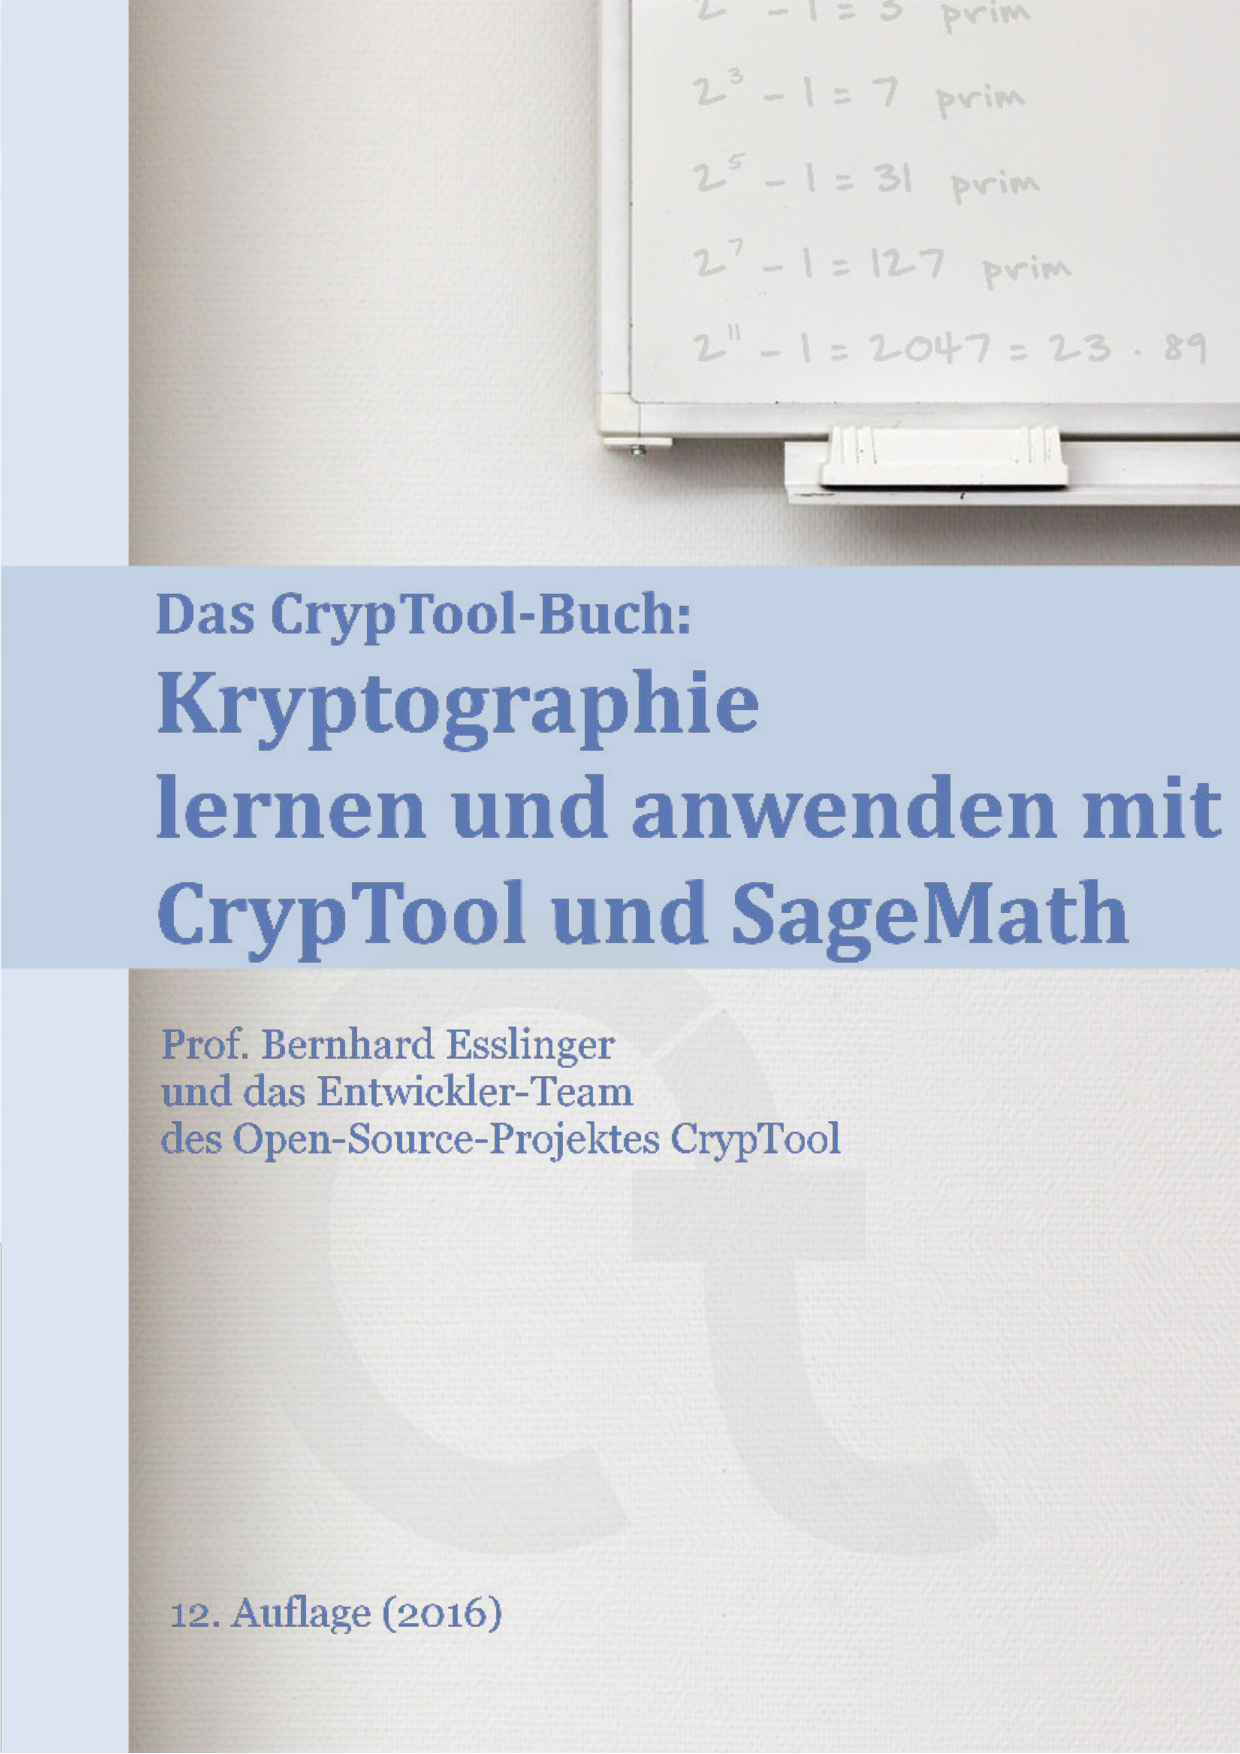
\includepdf[pages=1]{figures/coverv1_de_draft.pdf}  % 100dpi (kein Draftbalken mehr, nur geringere Aufl�sung)
% 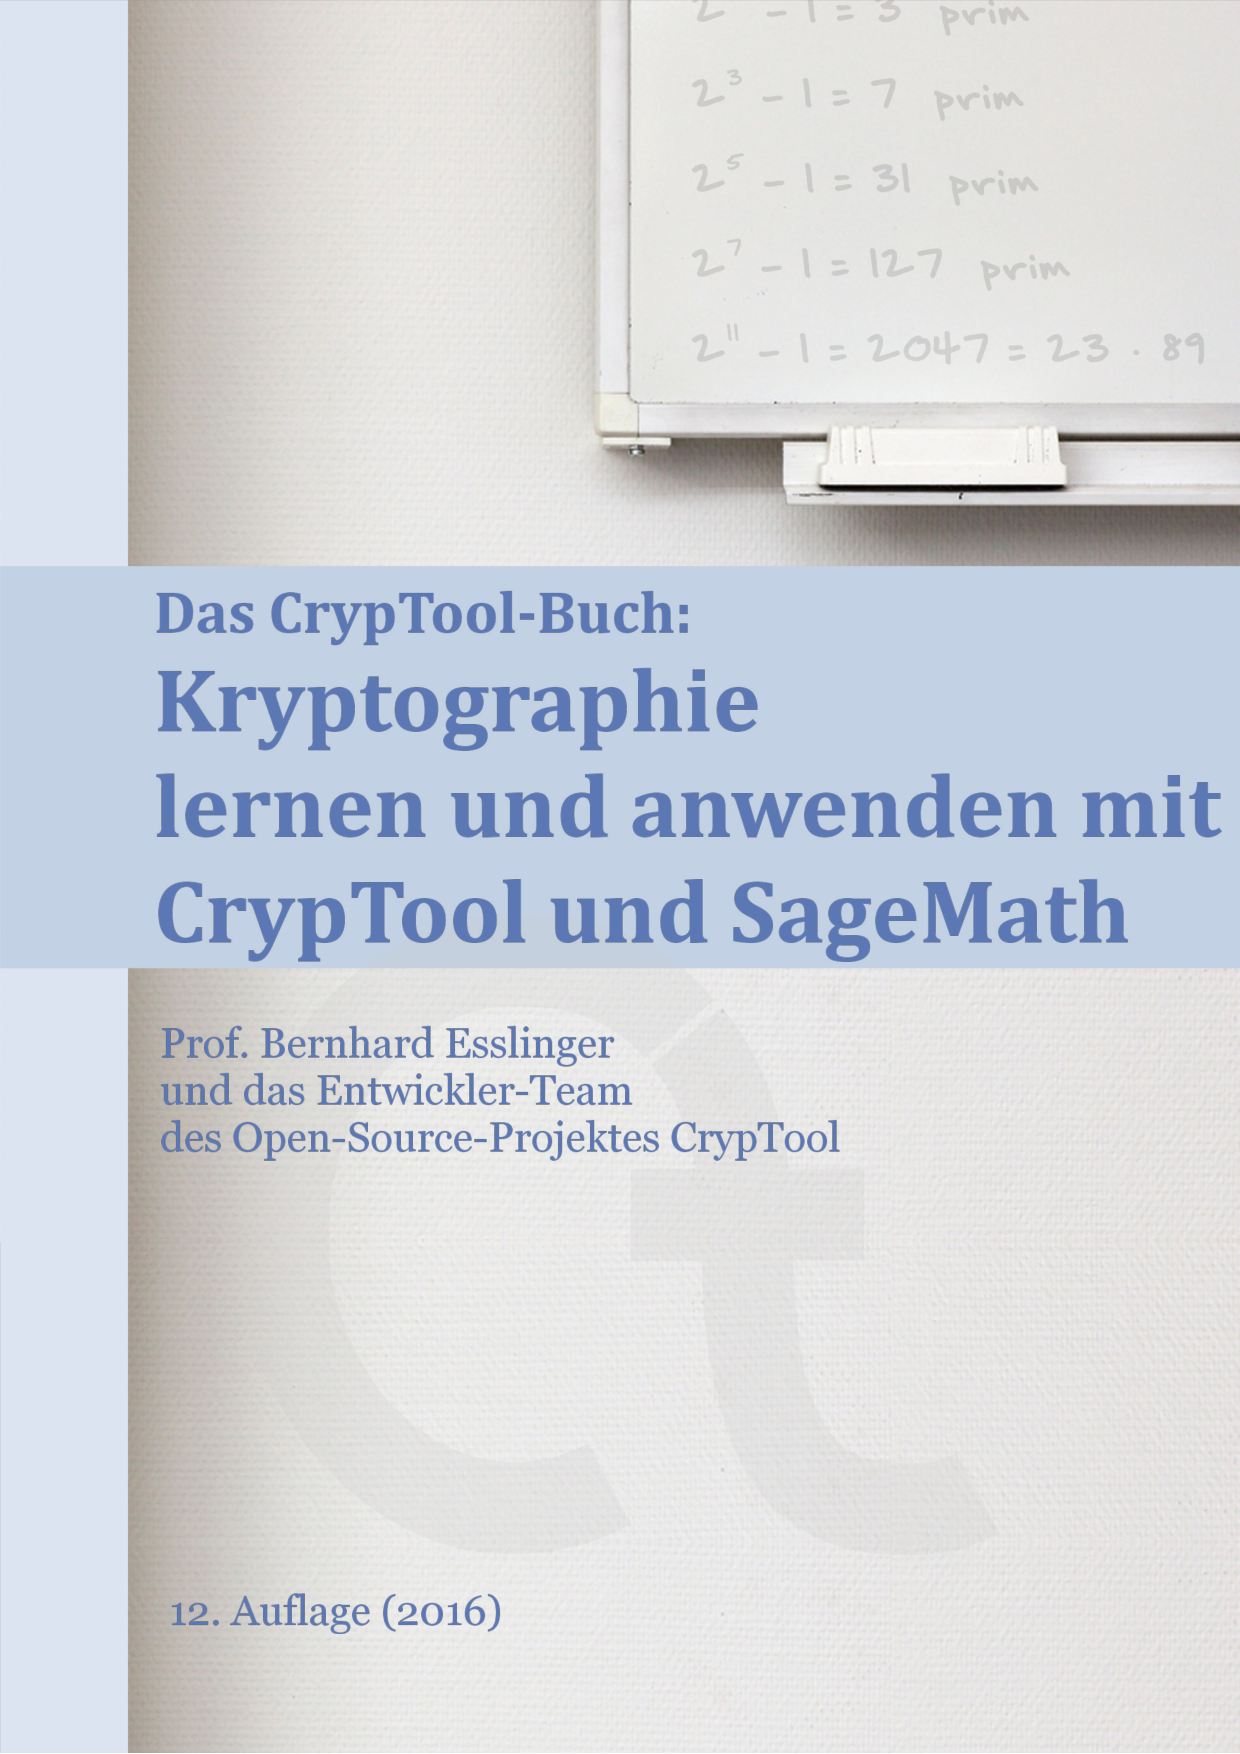
\includepdf[pages=1]{figures/coverv1_de.pdf}        % 300dpi (wieder pdf statt png)

\pagestyle{plain}
\setlength{\fboxrule}{.5mm}
\setlength{\fboxsep}{1.75mm}
\setlength{\footnotesep}{6pt}
\addtolength{\footskip}{8pt}
% \setlength{\footskip}{4cm}

\VerbatimFootnotes
% space between text and footnote 
% \renewcommand{\footnoterule}{\parindent0cm\rule{13cm}{.1pt}\vspace{.2cm}}
% Formatierung der Fu�noten
\renewcommand\footnoterule{
\vspace{2em}%   <-- one line space between text and footnoterule
% \kern-3\p@
\hrule width .4\columnwidth
\vspace{4pt}
% kern 2.6\p@
}

%\long\def\@makefntext#1{%
%\parindent 1em%
%\noindent
%\hbox to 1.8em{\hss\@makefnmark}#1}


\frontmatter % Ab hier beginnt Seitennummerierung mit r�mischen Ziffern
\maketitle


% Vergleichbar zur Nutzung von Texten aus der Wikipedia (=GNU Free Documentation Licence, GFDL)
\begin{quote}
Dies ist ein freies Dokument, d.h. Inhalte des Dokuments k�nnen kopiert und
verbreitet werden, auch zu kommerziellen Zwecken. \\
Im Gegenzug sind Autor, Titel und die CrypTool-Webseite (www.cryptool.org) zu
nennen. Selbstverst�ndlich darf aus dem CrypTool-Skript, genau wie aus jedem
anderen Werk auch, zitiert werden. \\
Dar�ber hinaus unterliegt dieses Dokument der GNU-Lizenz f�r freie
Dokumentation.

    Copyright \copyright{} 1998--2016 Bernhard Esslinger and the
    CrypTool Team. Permission is granted to copy,
    distribute and/or modify this document under the terms of the GNU
    Free Documentation License, Version 1.3 or any later version
    published by the Free Software Foundation. A copy of
    the license is included in the section entitled
    \hyperlink{appendix-GNU-fdl}{``GNU Free Documentation License''}.

    Dies beinhaltet auch den Code f�r die SageMath-Beispiele in diesem Dokument.
\end{quote}

\vspace{420pt}
\noindent
Quelle Coverfoto: \url{www.photocase.com}, Andre G�nther\\
Schriftsatz-Software: \LaTeX\\
Versionsverwaltungs-Software: Subversion


% be_2005: a) Auf erste Seite nur den Titel ! -> Newpage eingef�gt.
%          b) "aboutcryptool.tex" hier und nicht unten vor "introduction.tex"
%             einf�gen, damit es VOR dem Inhaltsverzeichnis steht.
% $Id: aboutcryptool.tex 3714 2016-04-08 18:34:16Z esslinger $
% ............................................................................
%                 TEXT DER 2. SEITE (�berblick)
%
% ~~~~~~~~~~~~~~~~~~~~~~~~~~~~~~~~~~~~~~~~~~~~~~~~~~~~~~~~~~~~~~~~~~~~~~~~~~~~

% HACK to fix warning "destination with the same identifier .. has already been used, ...":
% REMOVED, because it caused missing index entries
%\makeatletter \renewcommand{\thepage}{~\csname @roman\endcsname \c@page~} \makeatother
\clearpage\phantomsection
% HACK to fix warning "destination with the same identifier .. has already been used, ...":
% \makeatletter \renewcommand{\thepage}{\csname @roman\endcsname \c@page} \makeatother
% REMOVED, because it caused missing index entries
% BE_2016-03-16: Nahm dies ohne ~ nach "page" raus. Scheint nichts zu �ndern?

\addcontentsline{toc}{chapter}{�berblick �ber den Inhalt des CrypTool-Buchs}
\chapter*{�berblick �ber den Inhalt des CrypTool-Buchs}

\parskip 4pt
%\vskip +12 pt
Der Erfolg des Internets hat zu einer verst�rkten 
Forschung der damit verbundenen Technologien gef�hrt, was auch im
Bereich Kryptographie viele neue Erkenntnisse schaffte.

In diesem {\em Buch zu den CrypTool-Programmen} \index{CrypTool} finden Sie
eher mathematisch orientierte Informationen zum Einsatz von
kryptographischen Verfahren. Zu einigen Verfahren gibt es Beispielcode,
geschrieben f�r das Computer-Algebra-System {\bf SageMath}\index{SageMath}
(siehe Anhang~\ref{s:appendix-using-sage}).
Die Hauptkapitel sind von verschiedenen {\bf Autoren} verfasst
(siehe Anhang~\ref{s:appendix-authors}) %\hyperlink{appendix-authors}{Autoren}
und in sich abgeschlossen. Am Ende der meisten Kapitel finden Sie
Literaturangaben und Web-Links.
Die Kapitel wurden reichlich mit {\em Fu�noten} versehen, in denen auch darauf verwiesen
wird, wie man die beschriebenen Funktionen in den verschiedenen CrypTool-Programmen 
aufruft.

Das \hyperlink{Kapitel_1}{erste Kapitel} beschreibt die Prinzipien der
symmetrischen und asymmetrischen {\bf Verschl�sselung} und Definitionen f�r
deren Widerstandsf�higkeit.

Im \hyperlink{Kapitel_PaperandPencil}{zweiten Kapitel} wird -- aus 
didaktischen Gr�nden -- eine ausf�hrliche �bersicht
�ber {\bf Papier- und Bleistiftverfahren} gegeben.

Ein gro�er Teil des Buchs ist dem faszinierenden Thema der
{\bf Primzahlen} (Kapitel \ref{Label_Kapitel_Primes})
% \hyperlink{Kapitel_2}{{\bf Primzahlen}} 
gewidmet.
Anhand vieler Beispiele wird in die {\bf modulare Arithmetik} und die 
{\bf elementare Zahlentheorie} (Kapitel \ref{Chapter_ElementaryNT})
% \hyperlink{Chapter_ElementaryNT} {{\bf elementare Zahlentheorie}} 
eingef�hrt. Die Eigenschaften des {\bf RSA-Verfahrens} bilden einen Schwerpunkt. 

Danach erhalten Sie Einblicke in die mathematischen Konzepte und
Ideen hinter der
{\bf modernen Kryptographie} (Kapitel \ref{Chapter_ModernCryptography}).
%\hyperlink{Chapter_ModernCryptography}{{\bf modernen Kryptographie}}.

%Ein \hyperlink{Chapter_Hashes-and-Digital-Signatures}{weiteres Kapitel}
Kapitel \ref{Chapter_Hashes-and-Digital-Signatures} gibt
einen �berblick zum Stand der Attacken gegen moderne {\bf Hashalgorithmen}
und widmet sich dann kurz den {\bf digitalen Signaturen}
 --- sie sind unverzichtbarer Bestandteil von E-Business-Anwendungen.

%Das \hyperlink{ellcurve}{letzte Kapitel} stellt {\bf Elliptische Kurven} vor:
Kapitel \ref{Chapter_EllipticCurves} stellt {\bf Elliptische Kurven} vor:
Sie sind eine Alternative zu RSA und f�r die Implementierung auf Chipkarten
besonders gut geeignet.

Kapitel \ref{Chapter_BitCiphers} f�hrt in die {\bf Boolesche Algebra} ein.
Boolesche Algebra ist Grundlage der meisten modernen, symmetrischen
Verschl�sselungsverfahren, da diese auf Bitstr�men und Bitbl�cken operieren.
Prinzipielle Konstruktionsmethoden dieser Verfahren werden beschrieben
und in SagMath implementiert.


Kapitel \ref{Chapter_HomomorphicCiphers} stellt {\bf Homomorphe Kryptofunktionen}
vor: Sie sind ein modernes Forschungsgebiet, das insbesondere im Zuge des
Cloud-Computing an Bedeutung gewann.

Das \hyperlink{Chapter_Crypto2020}{letzte Kapitel} {\bf Krypto 2020}
diskutiert Bedrohungen f�r bestehende kryptographische Verfahren und 
stellt alternative Forschungsans�tze f�r eine langfristige
kryptographische Sicherheit vor.

W�hrend die CrypTool-\textit{eLearning-Programme}\index{eLearning} eher den
praktischen Umgang motivieren und vermitteln, dient das \textit{Buch} dazu, 
dem an Kryptographie Interessierten ein tieferes Verst�ndnis f�r die 
implementierten mathematischen Algorithmen zu vermitteln -- und das 
didaktisch m�g"-lichst gut nachvollziehbar. 

Die {\bf Anh�nge}
\ref{s:appendix-menu-overview-CT1},
\ref{s:appendix-template-overview-CT2},
\ref{s:appendix-function-overview-JCT} und
\ref{s:appendix-function-overview-CTO}
erlauben einen schnellen �berblick �ber die Funktionen in den verschiedenen
CrypTool-Varianten\index{CrypTool 1}\index{CrypTool 2}\index{JCrypTool} via:
\begin{itemize}
  \item der Funktionsliste und 
        dem \hyperlink{appendix-menu-overview-CT1}
                      {Men�baum von CrypTool 1 (CT1)},
  \item der Funktionsliste und 
        den \hyperlink{appendix-template-overview-CT2}
                      {Vorlagen in CrypTool 2 (CT2)},
  \item der \hyperlink{appendix-function-overview-JCT}
                      {Funktionsliste von JCrypTool (JCT)}, und
  \item der \hyperlink{appendix-function-overview-CTO}
                      {Funktionsliste von CrypTool-Online (CTO)}.
\end{itemize}
%Anker sind \hypertarget{appendix-menutree}{} und \label{s:appendix-menutree}
%  - \hyperlink{}{} legt Link auf die Seite unter den Text in 2. Klammer
%  - \ref{} legt Link und f�gt Kapitelnummer ein.

% Bernhard Esslinger, Matthias B�ger, Bartol Filipovic, Henrik Koy, Roger Oyono
% und J�rg Cornelius Schneider
Die Autoren m�chten sich an dieser Stelle bedanken bei den Kollegen 
in der jeweiligen Firma und an den Universit�ten Bochum, Darmstadt, Frankfurt,
Gie�en, Karlsruhe und Siegen.

\enlargethispage{0.5cm}
Wie auch bei dem E-Learning-Programm CrypTool\index{CrypTool} w�chst 
die Qualit�t des Buchs mit den Anregungen und Verbesserungsvorschl�gen 
von Ihnen als Leser. Wir freuen uns �ber Ihre R�ck"-mel"-dung.



% Local Variables:
% TeX-master: "../script-de.tex"
% End:
 % �berblick �ber den Inhalt des CT-Buches


\newpage
\pdfbookmark[0]{Kurzinhaltsverzeichnis}{ShortContents}
\shorttoc{Kurzinhaltsverzeichnis}{0}
\clearpage\phantomsection
\pdfbookmark[0]{\contentsname}{Contents}
\tableofcontents

\newpage
\normalsize

% \parindent 0cm
% \parskip 4pt
% Setting the default for the vertical distance before a paragraph as distinguished variable
\newcounter{mycounterDefaultParskip}
\setcounter{mycounterDefaultParskip}{4}
\parskip \value{mycounterDefaultParskip} pt 


% $Id: introduction.tex 3714 2016-04-08 18:34:16Z esslinger $
% ............................................................................
%      V O R W O R T  und  E I N F U E H R U N G (Zusammenspiel CT-Buch und CT-Programme) 
%      P R E F A C E  and  I N T R O D U C T I O N (Playing together of book and programs)
%
% ~~~~~~~~~~~~~~~~~~~~~~~~~~~~~~~~~~~~~~~~~~~~~~~~~~~~~~~~~~~~~~~~~~~~~~~~~~~~

\clearpage\phantomsection
% \vspace{-10pt}  wirkungslos!
\addcontentsline{toc}{chapter}{Vorwort zur 12. Auflage des CrypTool-Buchs}
\chapter*{Vorwort zur 12. Auflage des CrypTool-Buchs xxxxxxxxx}

%\vspace{-12pt}
Dieses Buch versucht, einzelne Themen aus der Mathematik der Kryptologie
genau, und trotzdem m�glichst verst�ndlich zu erl�utern.

Dieses Buch wurde ab dem Jahr 2000 -- zusammen mit dem CrypTool-1-Paket
(CT1)\index{CrypTool 1} in Version 1.2.01 -- ausgeliefert.
Seitdem ist das Buch mit fast jeder neuen Version von CT1 ebenfalls erweitert
und aktualisiert worden.

Themen aus Mathematik und Kryptographie wurden sinnvoll unterteilt und daf�r
wurden jeweils eigenst�ndig lesbare Kapitel geschrieben, damit 
Entwickler/Autoren unabh�ngig voneinander mitarbeiten k�nnen. Nat�rlich g�be
es viel mehr Themen aus der Kryptographie, die man vertiefen k�nnte -- deshalb
ist diese Auswahl auch nur eine von vielen m�glichen.

In der anschlie�enden redaktionellen Arbeit wurden in LaTeX Querverweise erg�nzt,
Fu�noten hinzugef�gt und Korrekturen vorgenommen.

%In dieser Ausgabe des CT-Buchs wurden wieder einige Themen auf den
%aktuellen Stand gebracht:
Im Vergleich zu Ausgabe 11 des Buchs wurden in dieser Ausgabe
% die TeX-Sourcen des Dokuments komplett �berarbei"-tet, und 
etliche Themen erg�nzt, korrigiert, und auf den aktuellen Stand gebracht, z.B.:
\vspace{-5pt}
\begin{itemize}
%  \item die Definitionen zur St�rke von Sicherheits-Funktionen
%        (Kapitel \ref{cm_Section_Security_Definitions}),
  \item die gr��ten Primzahlen (Kap. \ref{search_for_very_big_primes}),
%        neue Faktorisierungsrekorde (Kap. \ref{RSA-768}), und
%  \item Fortschritte bei der Kryptoanalyse von Hashverfahren 
%        (Kap. \ref{collision-attacks-against-sha-1}) und
%  \item Fortschritte bei den Ideen f�r neue Kryptoverfahren (RSA-Nachfolger)
%	(Kap. \ref{xxxxBrute-force-gegen-Symmetr})\index{xxxxxxxxxxxxxxxx} und
  \item die Auflistung, in welchen Filmen und Romanen Kryptographie eine
        wesentliche Rolle spielt (siehe Anhang \ref{s:appendix-movies}),
%       und Kurioses zu Primzahlen (siehe \ref{HT-Quaint-curious-Primes-usage}),
  \item die Funktions�bersichten
        \hyperlink{appendix-template-overview-CT2}{zu CrypTool 2 (CT2)},
        \hyperlink{appendix-function-overview-JCT}{zu JCrypTool (JCT)}, und
        \hyperlink{appendix-function-overview-CTO}{zu CrypTool-Online (CTO)}
        (siehe Anhang),
  \item weitere SageMath-Skripte zu Kryptoverfahren, und die Einf�hrung in das 
        Computer-Algebra-System (CAS) SageMath (siehe
        Anhang \ref{s:appendix-using-sage}),
        % Nguyen und Massierer (vgl. auch Kap.~\ref{ec:Sage_Massierer})
  \item der Abschnitt �ber die Goldbach-Vermutung
        (siehe \ref{L-GoldbachConjecture}) und �ber Primzahl-Zwillinge
        (siehe \ref{L-TwinCousinPrimes}),
  \item der Abschnitt �ber gemeinsame Primzahlen in real verwendeten
        RSA-Modulen (siehe \ref{nt_Shared-Primes}),
%  \item der Abschnitt �ber RSA-Fixpunkte
%        (siehe \ref{l:NumberTheory_Sage_Number-of-RSA-FixedPoints}), und
%  \item Homomorphe Verschl�sselung
%        (siehe Kapitel \ref{Chapter_HomomorphicCiphers})
  \item Die \nameref{Chapter_BitCiphers} ist v�llig neu
	(siehe Kapitel \ref{Chapter_BitCiphers}).
\end{itemize}

%Inzwischen bekommt das CT-Projekt Feedback und Testimonials aus nahezu allen
%L�ndern der Erde.


\newpage
\noindent \textbf{Dank}

An dieser Stelle m�chte ich explizit folgenden Personen danken, 
die bisher in ganz besonderer Weise zum CrypTool-Projekt\index{CrypTool} 
beigetragen haben.
Ohne ihre besonderen F�higkeiten und ihr gro�es Engagement w�re CrypTool
nicht, was es heute ist:
\vspace{-6pt}
\begin{list}{\textbullet}{\addtolength{\itemsep}{-0.5\baselineskip}}
   \item Hr.\ Henrik Koy
   \item Hr.\ J�rg-Cornelius Schneider
   \item Hr.\ Florian Marchal
   \item Dr.\ Peer Wichmann
   \item Hr.\ Dominik Schadow
   \item Mitarbeiter in den Teams von
         Prof.\ Johannes Buchmann,
         Prof.\ Claudia Eckert,
         Prof.\ Alexander May,
         Prof.\ Torben Weis und insbesondere
         Prof.\ Arno Wacker.
\end{list}

Auch allen hier nicht namentlich Genannten ganz herzlichen Dank f�r das 
(meist in der Freizeit) geleistete Engagement.

Danke auch an die Leser, die uns Feedback sandten. 

Ich hoffe, dass viele Leser mit diesem Buch mehr Interesse an und 
Verst�ndnis f�r dieses moderne und zugleich uralte Thema finden.



\par \vskip + 45pt
\noindent Bernhard Esslinger
\par \vskip + 10pt
\noindent Frankfurt/Siegen, April 2016



\par \vskip + 100pt
\noindent PS:\\
Wir w�rden uns freuen, wenn sich weitere Autoren finden, die fundierte
Artikel z.B. zu einem der folgenden Themen erg�nzen k�nnten:\\
- Riemannsche Zeta-Funktion,\\
- Hashverfahren,\\
- Gitter-basierte Kryptographie,\\
- Zufallszahlen oder\\
- Design/Angriff auf Krypto-Protokolle (wie SSL).
 
% [1.5\baselineskip]
% \enlargethispage*{2\baselineskip}
% \nopagebreak



% --------------------------------------------------------------------------
\clearpage\phantomsection
\addcontentsline{toc}{chapter}{Einf�hrung -- Zusammenspiel von Buch und Programmen}
\chapter*{Einf�hrung -- Zusammenspiel von Buch und Programmen}

\textbf{Das CrypTool-Buch}

Dieses Buch wird zusammen mit den Open-Source-Programmen des
CrypTool-Projektes\index{CrypTool} ausgeliefert.

Die Kapitel dieses Buchs sind weitgehend in sich abgeschlossen und k�nnen
auch unabh�ngig von den CrypTool-Programmen gelesen werden.

%W�hrend f�r das Verst�ndnis der meisten Kapitel Abiturwissen ausreicht,
%erfordern die Kapitel \ref{Chapter_ModernCryptography} (Moderne Kryptografie)
%und \ref{Chapter_EllipticCurves} (Elliptische Kurven) tiefere mathematische
%Kennt"-nisse.
F�r das Verst�ndnis der meisten Kapitel reicht Abiturwissen aus. Die Kapitel
\ref{Chapter_ModernCryptography} (\glqq Moderne Kryptografie\grqq), % (\glqq \nameref{Chapter_ModernCryptography}\grqq)
\ref{Chapter_EllipticCurves} (\glqq \nameref{Chapter_EllipticCurves}\grqq),
\ref{Chapter_BitCiphers} (\glqq Bitblock- und Bitstrom-Verschl�sselung\grqq) und % (\glqq \nameref{Chapter_BitCiphers}\grqq)
\ref{Chapter_HomomorphicCiphers} (\glqq \nameref{Chapter_HomomorphicCiphers}\grqq)
erfordern tiefere mathematische Kennt"-nisse.

Die \hyperlink{appendix-authors}{Autoren}
% \hyperlink{appendix-authors}{(Autoren)}
% in \ref{s:appendix-authors}
% \hypertarget{appendix-authors}{}\label{s:appendix-authors}
haben sich bem�ht, Kryptographie f�r eine m�glichst breite Leserschaft
darzu"-stellen -- ohne mathematisch unkorrekt zu werden. Sie wollen die
Awareness f�r die IT-Sicherheit und den Einsatz standardisierter, moderner
Kryptographie f�rdern.
\par \vskip + 15pt


\noindent \textbf{Die Programme CrypTool 1\index{CrypTool 1}\index{CT1},
  CrypTool 2\index{CrypTool 2}\index{CT2} und JCrypTool\index{JCrypTool}\index{JCT}}

CrypTool 1 (CT1) ist ein Lernprogramm mit umfangreicher
Online-Hilfe, mit dem Sie unter einer einheitlichen Oberfl�che
kryptographische Verfahren anwenden und analysieren k�nnen. Die Onlinehilfe in
CrypTool 1 enth�lt nicht nur Anleitungen zur Bedienung des Programms, sondern auch
Informationen zu den Verfahren selbst (aber weniger ausf�hrlich und anders
strukturiert als im CT-Buch).

CrypTool 1\index{CrypTool 1} und die Nachfolgeversionen
CrypTool 2 (CT2)\index{CrypTool 2} und JCrypTool (JCT)\index{JCrypTool}
werden weltweit in Schule, Ausbildung und Lehre eingesetzt.
\par \vskip + 15pt


\noindent \textbf{CrypTool-Online\index{CrypTool-Online}\index{CTO}}

Die Webseite CrypTool-Online (CTO) (\url{http://www.cryptool-online.org}), auf
der man im Browser oder vom Smartphone aus kryptographische Verfahren
ausprobieren und anwenden kann, geh�rt ebenfalls zum CT-Projekt. Der Umfang
von CTO ist bei weitem nicht so gro� wie der der Standalone-Programme CT1,
CT2 und JCT.
\par \vskip + 15pt


\noindent \textbf{MTC3\index{MTC3}}

Der internationale Kryptographie-Wettbewerb
MysteryTwister C3 (MTC3) (\url{http://www.mysterytwisterc3.org})
wird ebenfalls vom CT-Projekt getragen.
Hier findet man kryptographische R�tsel in vier verschiedenen Kategorien, eine
High-Score-Liste und ein moderiertes Forum. Inzwischen nehmen �ber 4000 aktive
Teilnehmer teil, und es gibt �ber 150 Aufgaben, von denen z.Zt. 109 von
zumindest einem Teilnehmer gel�st wurden.xxxxxxxxxxxxxxxx
\par \vskip + 15pt



\noindent \textbf{Das Computer-Algebra-Programm SageMath\index{SageMath}}

SageMath ist ein umfangreiches Open-Source CAS-Paket, mit dem sich die in
diesem Buch erl�uterten mathematischen Verfahren leicht Schritt-f�r-Schritt
programmieren lassen. Eine Besonderheit dieses CAS ist, dass als Skript-Sprache
Python benutzt wird.\\
SageMath wird mehr und mehr zum Standard-Open-Source CAS an Hochschulen.
\par \vskip + 15pt



\noindent \textbf{Die Sch�ler-Krypto-Kurse\index{Sch�ler-Krypto}}

Diese Initiative bietet Ein- und Zwei-Tages-Kurse in Kryptologie f�r Sch�ler
und Lehrer, um zu zeigen, wie attraktiv MINT-F�cher wie Mathematik,
Informatik und insbesondere Kryptologie sind.
Die Kursidee ist eine virtuelle Geheimagenten-Ausbildung.\\
Inzwischen finden diese Kurse seit mehreren Jahren in Deutschland in
unterschiedlichen St�dten statt.\\
Alle Kursunterlagen sind frei erh�ltlich
(\url{http://www.cryptool.org/schuelerkrypto/}).\\
Alle eingesetzte Software ist ebenfalls frei (meist wird CT1 und CT2
eingesetzt).\\
Wir w�rden uns freuen, wenn jemand die Kursunterlagen �bersetzt und
einen entsprechenden Kurs in Englisch anbieten w�rde.
\par \vskip + 15pt



\noindent \textbf{Dank}

Herzlichen Dank an alle, die mit ihrem gro�em Einsatz zum 
Erfolg und zur weiten Verbreitung dieses Projekts beigetragen haben.



\par \vskip + 45pt
\noindent Bernhard Esslinger
\par \vskip + 10pt
\noindent Frankfurt/Siegen, April 2016

% Local Variables:
% TeX-master: "../script-de.tex"
% End:
 % Working together of Book and Programm 

\mainmatter % Ab hier beginnt Seitennummerierung mit arabischen Ziffern
% $Id: cryptomethods.tex 3716 2016-04-10 20:16:26Z esslinger $
% ............................................................................
%             V E R S C H L U E S S E L U N G S V E R F A H R E N
%
% ~~~~~~~~~~~~~~~~~~~~~~~~~~~~~~~~~~~~~~~~~~~~~~~~~~~~~~~~~~~~~~~~~~~~~~~~~~~~

% HACK to fix warning "destination with the same identifier .. has already been used, ...":
% REMOVED, because it caused missing index entries
%\makeatletter \renewcommand{\thepage}{~\csname @arabic\endcsname \c@page} \makeatother

\hypertarget{Kapitel_1}{}
\chapter{Sicherheits-Definitionen und Verschl�sselungsverfahren}
\label{Label_Kapitel_1}
(Bernhard Esslinger, J�rg-Cornelius Schneider, Mai 1999; Updates: Dez. 2001, Feb. 2003, Juni 2005, Juli 2007, Jan. 2010, M�rz 2013, M�rz 2016)

Dieses Kapitel soll einen eher beschreibenden Einstieg bieten und die
Grundlagen ohne Verwendung von allzu viel Mathematik vermitteln.

Sinn der Verschl�sselung \index{Verschl�sselung} ist es, Daten so zu
ver�ndern, dass nur ein autorisierter Empf�n\-ger in der Lage ist,
den Klartext zu rekonstruieren. Das hat den Vorteil, dass verschl�sselte
Daten offen �bertragen werden k�nnen und trotzdem keine Gefahr besteht,
dass ein Angreifer die Daten unberechtigterweise lesen kann. Der
autorisierte Empf�nger ist im Besitz einer geheimen Information, des
sogenannten Schl�ssels, die es ihm erlaubt, die Daten zu entschl�sseln,
w�hrend sie jedem anderen verborgen bleiben.%\par \vskip + 3pt

Zur Erl�uterung verwenden wir im Folgenden die Begriffe aus der
Abbildung \ref{Generic-Notations-when-Encrypting}:
\begin{figure}[ht]
\begin{center}
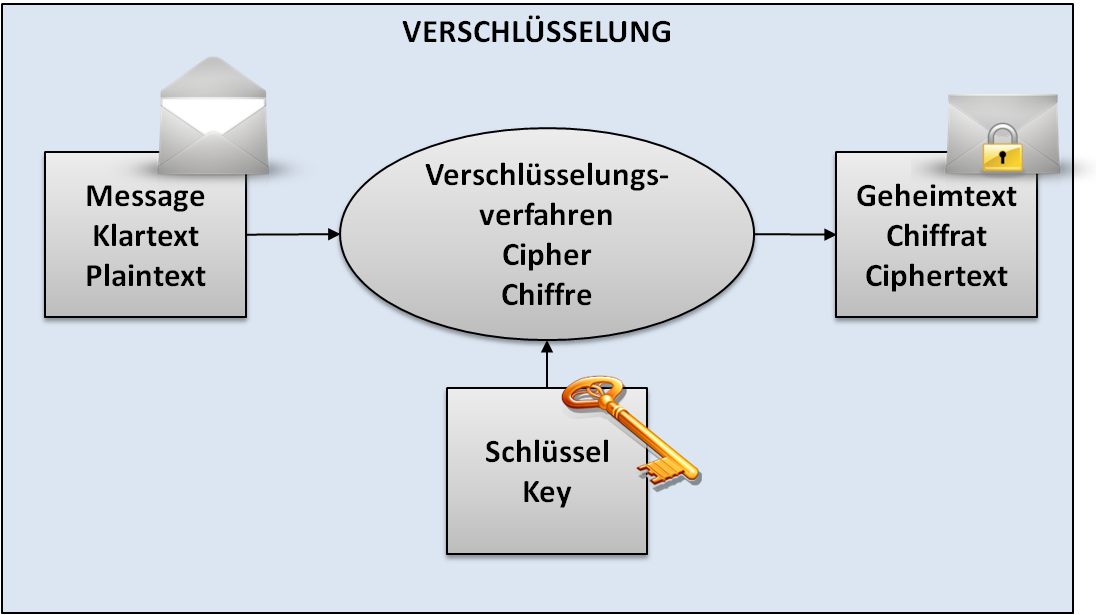
\includegraphics[scale=0.7]{figures/Generic-Notation-Encryption_de.png}
\caption{�bliche Bezeichnungen bei der Verwendung von Verschl�sselungsverfahren} 
\label{Generic-Notations-when-Encrypting}
\end{center}
\end{figure}


Zuerst erkl�ren wir, wie die Sicherheit von Kryptosystemen definiert wird.



% --------------------------------------------------------------------------
\hypertarget{cm_Section_Security_Definitions}{}
\section[Sicherheits-Definitionen]{Sicherheits-Definitionen}
\label{cm_Section_Security_Definitions}
\index{Sicherheits-Definitionen}

\begin{ctsquote}
Erkl�re es mir, ich werde es vergessen.\\
Zeige es mir, ich werde es vielleicht behalten.\\
Lass es mich tun, und ich werde es k�nnen.
\caption{Indisches Sprichwort}
\end{ctsquote}

Moderne Kryptographie basiert vor allem auf mathematischer Theorie und
Computer-Praxis. Beim Design kryptographischer Algorithmen werden Annahmen
zur Schwierigkeit von Berechnungen so gemacht, so dass sich solche Verfahren
in der Praxis von einem Angreifer nur schwer brechen lassen.

\vskip +3pt
Die zwei Hauptnotationen in der Literatur definieren Sicherheit in
Abh�ngigkeit von den M�glichkeiten des Angreifers (vgl. z.B.
{\em Contemporary Cryptography} \cite{cm:Oppliger2011}):

\begin{itemize}

\item {\bf Berechenbare, bedingte oder praktische Sicherheit}\\
Ein Verschl�sselungsverfahren ist berechenbar sicher, wenn es (obwohl es
theoretisch m�glich ist, es zu brechen) selbst mit den besten bekannten
Verfahren nicht gebrochen werden kann. Theoretische Fortschritte (z.B.
Verbesserungen bei den Algorithmen zur Faktorisierung) und schnellere
Computer erfordern, dass dies st�ndig angepasst wird. 

Selbst wenn man den besten bekannten Algorithmus zum Brechen benutzt, wird
man so viele Ressourcen brauchen (z.B. 1.000.000 Jahre), dass das Kryptosystem
sicher ist.

Daher basiert dieses Konzept auf Annahmen �ber die begrenzte Rechenkraft des
Angreifers und auf dem aktuellen Stand der Wissenschaft.

\item {\bf Informations-theoretische oder unbedingte Sicherheit}\\
Ein Verschl�sselungsverfahren ist unbedingt sicher, wenn es sicher ist, v�llig
unabh�ngig davon, wieviele Ressourcen (Zeit, Speicher) der Angreifer hat, also
auch in dem Fall, wenn der Angreifer unbegrenzt viele Ressourcen hat, um das
Verfahren zu brechen. Ein Angreifer hat nicht genug Informationen daf�r, weil
sich aus dem Chiffrat keine sinnvollen Informationen gewinnen lassen.

Es gibt Informations-theoretisch sichere Verfahren, die beweisbar nicht
gebrochen werden k�nnen, auch nicht mit unendlich viel Rechenkraft -- ein
Beispiel daf�r ist das {\em One-Time-Pad}\index{One-Time-Pad} (OTP\index{OTP}).

Da das OTP ein Informations-theoretisch sicheres Verschl�sselungsverfahren
ist, leitet sich seine Sicherheit schon allein aus der Informationstheorie
ab -- und ist sicher, auch wenn der Angreifer unbegrenzte Rechenkapazit�ten
hat. Das OTP weist allerdings einige praktische Nachteile auf (der
verwendete Schl�ssel darf nur einmal verwendet werden, muss zuf�llig
gew�hlt werden und mindestens so lang sein wie die zu sch�tzende Nachricht),
so dass es au�er in geschlossenen Umgebungen, zum Beispiel beim hei�en
Draht zwischen Moskau und Washington, kaum eine Rolle spielt.%\par \vskip + 3pt

\end{itemize}


\vskip +3pt
\noindent Manchmal werden auch zwei weitere Konzepte verwendet:

\begin{itemize}

\item {\bf Beweisbare Sicherheit}
Dies bedeutet, dass das Brechen eines Kryptosystems mindestens so schwierig ist
wie die L�sung eines bestimmten schwierigen Problems, z.B. die Berechnung des
diskreten Logarithmus, die diskrete Quadratwurzel-Berechnung oder die
Faktorisierung sehr gro�er Zahlen.

Beispiel: Aktuell wissen wir, dass RSA\index{RSA} h�chstens so schwierig
ist wie die Faktorisierung, aber wir k�nnen nicht beweisen, dass es genauso
schwierig ist.
Deshalb hat RSA keine beweisbare Mindest-Sicherheit. Oder in anderen Worten:
Wir k�nnen nicht beweisen, dass wenn das Kryptosystem RSA gebrochen ist, dass
dann auch die Faktorisierung (ein schwieriges mathematisches Problem) gel�st
werden kann.

Das Rabin-Kryptosystem war das erste Kryptosystem, f�r das sich beweisen lie�,
dass es berechenbar �quivalent zu einem harten mathematischen Problem ist.

\item {\bf Ad-hoc-Sicherheit}
Ein kryptographisches System hat diese Sicherheit, wenn es sich nicht lohnt,
es zu versuchen es zu brechen, weil der Aufwand daf�r teurer ist als der Wert
der Daten, die man durch das Brechen erhalten w�rde. Z.B. weil ein Angriff
nicht in einer ausreichend kurzen Zeit erfolgen kann (vgl.
{\em Handbook of Applied Cryptography} \cite{cm:Menezes2001}).

Dies kann z.B. zutreffen, wenn B�rsen-relevante Daten sowieso am
n�chsten Tag ver�ffent"-licht werden und man f�r das Brechen ein Jahr brauchen
w�rde.

\end{itemize}


\vskip +3pt
Bei den heutzutage verwendeten guten Verfahren ist der Zeitaufwand zum Brechen
so hoch, dass sie praktisch nicht gebrochen werden k�nnen. Deshalb kann man
diese Verfahren als (praktisch) sicher ansehen -- aus einer rein auf den
Algorithmus bezogenen Sichtweise.%\par

\vskip +3pt
\begin{sloppypar}
Grunds�tz"-lich unterscheidet man zwischen symmetrischen und asymmetrischen
Verfahren zur Verschl�sse"-lung.
Einen guten �berblick �ber die verschiedenen Verschl�sselungs-Verfahren bietet
das Buch von Bruce Schneier \cite{cm:Schneier1996}.
\end{sloppypar}
\vskip +3pt





% --------------------------------------------------------------------------
\newpage

\begin{ctsquote}
\glqq Man kann nicht nicht kommunizieren!\grqq 
\caption[Paul Watzlawick]{Paul Watzlawick\footnotemark}\index{Watzlawick, Paul}
\end{ctsquote}
\addtocounter{footnote}{0}\footnotetext{Paul Watzlawick, Janet H. Beavin und Don D. Jackson, \glqq Menschliche Kommunikation. Formen, St�rungen, Paradoxien\grqq, Huber, (c) 2007, Das erste der f�nf pragmatischen Axiome ihrer Kommunikationstheorie.}

% --------------------------------------------------------------------------
\section[Einfl�sse auf Verschl�sselungsverfahren] % Was zw. [..] steht, kommt ins Inhaltsverzeichnis!
{Einfl�sse auf Verschl�sselungsverfahren}

% \nopagebreak
Hier sollen kurz zwei Aspekte von Kryptoverfahren erw�hnt werden, auf die oft nicht fr�h genug eingegangen wird:

\begin{itemize}

\item {\bf Zufallsbasiert}\\
\index{Zufall}
Man kann Algorithmen trennen in deterministische\index{deterministisch} und heuristische\index{heuristisch} Verfahren. Meistens lernten Studenten nur deterministische Verfahren kennen, bei denen die Ausgabe eindeutig durch die Eingabe vorgegeben wird. Bei heuristischen Verfahren werden Entscheidungen aufgrund zuf�lliger Werte getroffen. Moderne Verfahren des maschinellen Lernens geh�ren ebenfalls hierzu.

In Kryptoverfahren spielt Zufall eine gro�e Rolle. Immer m�ssen die Schl�ssel zuf�llig gew�hlt werden, so dass zumindest bei der Schl�sselgenerierung~\glqq Zufall\grqq~erzeugt werden muss. Zus�tzlich sind manche Verfahren (vor allem aus der Kryptoanalyse) heuristisch.

\item {\bf Konstanten-basiert}\\
Viele moderne Verfahren (insbesondere Hashverfahren und symmetrische Verschl�sse-lungsverfahren) benutzen numerische Konstanten. Diese sollten nachvollziehbar sein und keine Hintert�ren erm�glichen. Zahlen, die das erf�llen, nennt man im Englischen~\glqq Nichts-im-�rmel\grqq-Zahlen: Nothing-up-my-sleeve number\index{Zahlen!Nothing-up-my-sleeve}.%
\footnote{\url{http://en.wikipedia.org/wiki/Nothing_up_my_sleeve_number}}

\end{itemize}









% --------------------------------------------------------------------------
\newpage

\begin{ctsquote}
\glqq Transparenz. Das ist das H�chste, was man sich in einer technologisch hoch entwickelten Gesellschaft erhoffen kann ... sonst wird man einfach nur manipuliert.\grqq 
\caption[Daniel Suarez]{Daniel Suarez\footnotemark}\index{Suarez, Daniel}
\end{ctsquote}
\addtocounter{footnote}{0}\footnotetext{Daniel Suarez, \glqq Darknet\grqq,
            rororo, (c) 2011, Kapitel 5, \glqq Einsichten\grqq, S. 69, Price.}

% --------------------------------------------------------------------------
\section[Symmetrische Verschl�sselung] % Was zw. [..] steht, kommt ins Inhaltsverzeichnis!
{Symmetrische Verschl�sselung\footnotemark}
  \footnotetext{% Dieses Prozent ist n�tig, sonst startet die Fu�note mit einem Blank !
    Mit CrypTool 1 ({\bf CT1})\index{CT1}\index{CrypTool 1} k�nnen Sie �ber das
    Men� {\bf Ver-/Entschl�sseln \textbackslash{} Symmetrisch (modern)} folgende
    modernen symmetrischen Verschl�sselungsverfahren ausf�hren:\\
    IDEA, RC2, RC4, DES (ECB), DES (CBC), Triple-DES (ECB), Triple-DES (CBC),
    MARS (AES-Kandidat), RC6 (AES-Kandidat), Serpent (AES-Kandidat), 
    Twofish (AES-Kandidat),
    Rijndael (offizielles AES-Verfahren)\index{AES}.\\
    Mit CrypTool 2 ({\bf CT2})\index{CT2}\index{CrypTool 2} k�nnen Sie im Startcenter
    �ber {\bf Vorlagen \textbackslash{} Kryptographie \textbackslash{}
    Modern \textbackslash{} Symmetrisch} folgende modernen symmetrischen
    Verschl�sselungsverfahren ausf�hren:\\ 
    AES, DES, PRESENT, RC2, RC4, SDES, TEA, Triple-DES, Twofish.\\
    In JCrypTool ({\bf JCT})\index{JCT}\index{JCrypTool} stehen Ihnen die folgenden
    modernen symmetrischen Verschl�sselungsverfahren zur Verf�gung:\\ 
    AES, Rijndael, Camellia, DES, Dragon, IDEA, LFSR, MARS, Misty1, RC2, RC5,
    RC6, SAFER+, SAFER++, Serpent, Shacal, Shacal2, Twofish.
    }

\nopagebreak

Bei der {\em symmetrischen} Verschl�sselung 
\index{Verschl�sselung!symmetrisch} m�ssen Sender und Empf�nger
�ber einen gemeinsamen (geheimen) Schl�ssel verf�gen, den sie vor
Beginn der eigentlichen Kommunikation ausgetauscht haben. Der Sender
benutzt diesen Schl�ssel, um die Nachricht zu verschl�sseln und der
Empf�nger, um diese zu entschl�sseln.\par %\vskip + 3pt

Dies veranschaulicht Abbildung \ref{Figure_Symmetric-Enc_Secret-Key-Enc}:
\begin{figure}[ht]
\begin{center}
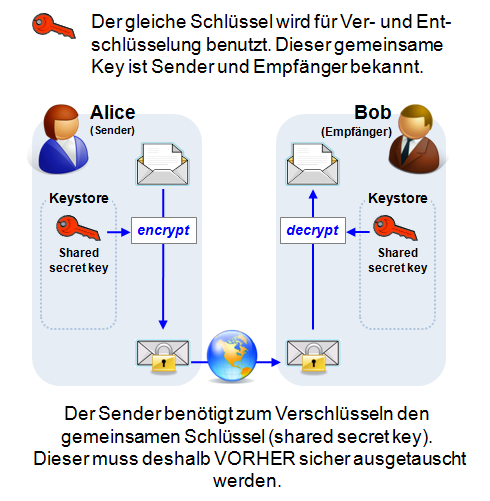
\includegraphics[scale=0.7]{figures/SymmetricEnc_Figure_Chap1_de.png}
\caption{Symmetrische oder Secret-Key-Verschl�sselung} 
\label{Figure_Symmetric-Enc_Secret-Key-Enc}
\end{center}
\end{figure}

Alle klassischen Chiffren sind vom Typ symmetrisch. Beispiele dazu finden Sie
in den CT-Programmen, im Kapitel~\ref{Kapitel_PaperandPencil}
(\glqq \nameref{Kapitel_PaperandPencil}\grqq )
in diesem Skript oder in \cite{cm:Nichols1996}. 
In diesem Unterkapitel wollen wir jedoch nur die moderneren symmetrischen
Verfahren betrachten.

Vorteile von symmetrischen Algorithmen sind die hohe
Geschwindigkeit, mit denen Daten ver- und entschl�sselt werden.
Ein Nachteil ist das Schl�sselmanagement. Um miteinander
vertraulich kommunizieren zu k�nnen, m�ssen Sender und
Empf�nger vor Beginn der eigentlichen Kommunikation �ber einen
sicheren Kanal einen Schl�ssel ausgetauscht haben. Spontane
Kommunikation zwischen Personen, die sich vorher noch nie begegnet
sind, scheint so nahezu unm�glich. Soll in einem Netz mit $ n $
Teilnehmern jeder mit jedem zu jeder Zeit spontan kommunizieren
k�nnen, so muss jeder Teilnehmer vorher mit jedem anderen der
$n - 1$ Teilnehmer einen Schl�ssel ausgetauscht haben. Insgesamt
m�ssen also $n(n - 1)/2$ Schl�ssel ausgetauscht werden.\par \vskip + 3pt

Vor AES war der DES-Algorithmus\index{DES} das bekannteste symmetrische
Verschl�sselungs"-ver"-fahren. Der DES-Algorithmus ist eine Entwicklung von IBM 
in Zusammenarbeit mit der National Security Agency \index{NSA} (NSA). 
Er wurde 1975 als Standard ver�ffentlicht. Trotz seines relativ hohen
Alters ist jedoch bis heute kein ~\glqq effektiver\grqq~ Angriff auf
ihn gefunden worden. Der effektivste Angriff besteht aus dem Durchprobieren
(fast) aller m�glichen Schl�ssel, bis der richtige gefunden wird 
({\em Brute-Force-Angriff})\index{Angriff!Brute-Force}. Aufgrund der relativ
kurzen Schl�ssell�nge von effektiv 56 Bits (64 Bits, die allerdings 8
Parit�tsbits enthalten), sind in der Vergangenheit schon mehrfach mit dem
DES verschl�sselte Nachrichten gebrochen worden, so dass er heute nicht
mehr als sicher anzusehen ist. Alternativen zum DES sind zum Beispiel die
Algorithmen IDEA\index{IDEA}, Triple-DES und vor allem AES.
\par \vskip + 3pt

Standard unter den symmetrischen Verfahren ist heute AES\index{AES}:
Der dazu geh�rende Rijndael-Algo"-rithmus wurde am 2. Oktober 2000 zum
Gewinner der AES-Ausschreibung erkl�rt und ist damit Nachfolger
des DES-Verfahrens.

N�heres und weitere Verweise zum AES-Algorithmus und den AES-Kandidaten
der letzten Runde finden Sie z.B. in der Online-Hilfe von
CrypTool\index{CrypTool}.%
\footnote{%
      Online-Hilfe von CT1\index{CrypTool 1}: Das Stichwort {\bf AES} im Index
      f�hrt auf die drei Hilfeseiten: {\bf AES-Kandidaten}, 
      {\bf Der AES-Gewinner Rijndael} und {\bf Der AES-Algorithmus Rijndael}.\\
      Eine ausf�hrliche Beschreibung von AES mit C-Code findet sich
       in \cite{cm:Haan2008}.
  }




% HACK to fix warning "destination with the same identifier .. has already been used, ...":
% REMOVED, because it caused missing index entries
%\makeatletter \renewcommand{\thepage}{\csname @arabic\endcsname \c@page} \makeatother
% --------------------------------------------------------------------------
\subsection{Ergebnisse zur Kryptoanalyse von AES}
\label{NeueAES-Analyse}
\index{Kryptoanalyse}
\index{AES}

Im Anschluss finden Sie einige Informationen, die das AES-Verfahren in
letzter Zeit in Zweifel zogen -- unserer Ansicht nach aber (noch)
unbegr�ndet. Die folgenden Informationen beruhen vor allem auf den unten
angegebenen Originalarbeiten und auf \cite{cm:Wobst-iX2002} und
\cite{cm:Lucks-DuD2002}.

Der AES bietet mit einer Mindestschl�ssell�nge von 128 Bit gegen
Brute-Force-Angriffe auch auf l�ngere Sicht gen�gend Sicherheit -- es sei
denn, es st�nden entsprechend leistungsf�hige Quantencomputer zur
Verf�gung. Der AES war immun gegen alle bis dahin bekannten
Krypto"-analyse-Verfahren, die vor allem auf statistischen
�berlegungen beruhen und auf DES angewandt wurden: man konstruiert aus
Geheim- und Klartextpaaren Ausdr�cke, die sich nicht rein zuf�llig
verhalten, sondern R�ckschl�sse auf den verwendeten Schl�ssel zulassen.
Dazu waren aber unrealistische Mengen an abgeh�rten Daten n�tig.

Bei Kryptoverfahren bezeichnet man solche Kryptoanalyseverfahren als
"`akademischen Erfolg"' oder als "`kryptoanalytischen Angriff"', da sie
theoretisch schneller sind als das Durchprobieren aller Schl�ssel, das
beim Brute-Force-Angriff\index{Angriff!Brute-Force} verwendet wird. Im
Fall des AES mit maximaler Schl�ssell�nge (256 Bit) braucht die
ersch�pfende Schl�sselsuche im Durchschnitt $2^{255}$
Verschl�sselungsoperationen. Ein kryptoanalytischer Angriff muss diesen
Wert unterbieten. Als aktuell gerade noch praktikabel (z.B. f�r einen
Geheimdienst) gilt ein Aufwand von $2^{75}$ bis $2^{90}$
Verschl�sselungsoperationen.

Eine neue Vorgehensweise wurde in der Arbeit von Ferguson, Schroeppel
und Whiting im Jahre 2001 \cite{cm:Ferguson2001} beschrieben: Sie stellten
AES als geschlossene Formel (in der Form einer Art Kettenbruch) dar,
was aufgrund seiner "`relativ"' �bersichtlichen Struktur gelang. Da
diese Formel aus rund 1 Billiarde Summanden besteht, taugt sie zun�chst
nicht f�r die Kryptoanalyse. Dennoch war die wissenschaftliche Neugier
geweckt. Bereits bekannt war, dass sich der 128-Bit-AES als ein
�berbestimmtes System von rund 8000 quadratischen Gleichungen
(�ber algebraischen Zahlk�rpern) mit rund 1600 Variablen (einige
Unbekannte sind die Schl�sselbits) darstellen l�sst -- solch gro�e
Gleichungssysteme sind praktisch nicht l�sbar. Dieses Gleichungssystem
ist relativ d�nn besetzt (\glqq sparse\grqq), d.h. von den insgesamt etwa
1.280.000 m�glichen quadratischen Termen tauchen nur relativ wenige
�berhaupt im Gleichungssystem auf.

Die Mathematiker Courtois und Pieprzyk \cite{cm:Courtois2002} ver�ffentlichten 
2002 eine Arbeit, die in der Krypto-Szene stark diskutiert wird: Sie 
entwickelten das auf der Eurocrypt 2000 von Shamir et al. vorgestellte 
XL-Verfahren (eXtended Linearization) weiter zum XSL-Verfahren 
(eXtended Sparse Linearization). Das XL-Verfahren ist eine heuristische 
Technik, mit der es manchmal gelingt, gro�e nicht-lineare Gleichungssysteme 
zu l�sen und die bei der Analyse eines asymmetrischen Algorithmus (HFE) 
angewandt wurde.  Die Innovation von Courtois und Pieprzyk war, das 
XL-Verfahren auf symmetrische Verfahren anzuwenden: Das XSL-Verfahren kann
auf spezielle Gleichungssysteme angewandt werden. Damit k�nnte ein 
256-Bit-AES-Verfah"-ren in rund $2^{230}$ Schritten geknackt werden. Dies ist 
zwar immer noch ein rein akademischer Angriff, aber er ist richtungsweisend
f�r eine ganze Klasse von Blockchiffren. Das generelle Problem mit diesem
Angriff besteht darin, dass man bisher nicht angeben kann, unter welchen
Umst�nden er zum Erfolg f�hrt: die Autoren geben in ihrer Arbeit notwendige
Bedingungen an; es ist nicht bekannt, welche Bedingungen hinreichend sind.
Neu an diesem Angriff war erstens, dass dieser Angriff nicht auf Statistik,
sondern auf Algebra beruhte. Dadurch erscheinen Angriffe m�glich, die nur
geringe Mengen von Geheimtext brauchen. Zweitens steigt damit die Sicherheit
eines Produktalgorithmus%
\index{Produktalgorithmus}\index{Verschl�sselung!Produktalgorithmus}%
\footnote{%
Ein Geheimtext kann selbst wieder Eingabe f�r eine Chiffrierung sein. Eine
Mehrfachverschl�sselung (cascade cipher)
\index{Verschl�sselung!Mehrfachverschl�sselung}\index{Mehrfachverschl�sselung}
\index{Kaskaden}
entsteht aus einer Komposition von mehreren Verschl�sselungstransformationen.
Die Gesamtchiffrierung wird Produktalgorithmus oder Kaskadenalgorithmus
genannt (manchmal ist die Namensgebung abh�ngig davon, ob die verwendeten
Schl�ssel statistisch abh�ngig oder unabh�ngig sind).\\
Nicht immer wird die Sicherheit eines Verfahrens durch Produktbildung 
erh�ht.\\
Dieses Vorgehen wird auch {\em innerhalb} moderner Algorithmen angewandt:
Sie kombinieren in der Regel einfache und, f�r sich genommen, kryptologisch
relativ unsichere Einzelschritte in mehreren Runden zu einem leistungsf�higen
Gesamtverfahren. Die meisten modernen Blockchiffrierungen (z.B. DES, IDEA)
sind Produktalgorithmen.\\
Als Mehrfachverschl�sselung wird auch das Hintereinanderschalten desselben
Verfahrens mit verschiedenen Schl�sseln wie bei Triple-DES bezeichnet. 
}
nicht mehr exponentiell mit der Rundenzahl.

Aktuell wird sehr intensiv auf diesem Gebiet geforscht: z.B. stellten
Murphy und Robshaw auf der Crypto 2002 ein Papier vor \cite{cm:Robshaw2002a},
das die Kryptoanalyse drastisch verbessern k�nnte: Der Aufwand f�r
128-Bit-Schl�ssel wurde auf $2^{100}$ gesch�tzt, indem sie AES als
Spezialfall eines Algorithmus BES (Big Encryption System) darstellten,
der eine besonders "`runde"' Struktur hat. Aber auch $2^{100}$
Rechenschritte liegen jenseits dessen, was praktisch in absehbarer Zeit
realisierbar ist. Bei 256 Bit Schl�ssell�nge sch�tzen die Autoren
den Aufwand f�r den XSL-Angriff auf $2^{200}$ Operationen.

Weitere Details finden Sie unter den Weblinks bei
\hyperlink{CM_HT_Weblink_Rijndael-Cryptosystem}{\glqq Das AES-/Rijndael-Kryptosystem\grqq}.
% nur \href oder \url r�ckt nicht ein, deshalb \item dazu !
%\vspace{-10pt}
%\begin{itemize}
%  \item[] \url{http://www.cryptosystem.net/aes} \\
%          \url{http://www.minrank.org/aes/} 
%\end{itemize}


F�r AES-256 w�re der Angriff ebenfalls viel besser als
Brute-Force\index{Angriff!Brute-Force}, aber auch noch weiter au�erhalb der
Reichweite realisierbarer Rechenpower.

\begin{sloppypar}
Die Diskussion ist z.Zt. sehr kontrovers: Don Coppersmith (einer der
DES-Erfinder) z.B. bezweifelt die generelle Durchf�hrbarkeit des Angriffs:
XLS liefere f�r AES gar keine L�sung \cite{cm:Coppersmith2002}. Dann w�rde
auch die Optimierung von Murphy und Robshaw \cite{cm:Robshaw2002b} nicht
greifen.
\end{sloppypar}

2009 ver�ffentlichten Biryukov und Khovratovich \cite{cm:Biryukov2009} einen
weiteren theoretischen Angriff auf AES, der sich anderer Techniken bedient, als
die oben vorgestellten. Sie verwenden Methoden aus der Kryptoanalyse von
Hashfunktionen (lokale Kollisionen und das Boomerang-Verfahren) und
konstruierten daraus einen Related-Key-Angriff auf AES-256. D.~h.\ der Angreifer
muss nicht nur in der Lage sein, beliebige Daten zu verschl�sseln (chosen plain
text), sondern auch den ihm unbekannten Schl�ssel manipulieren k�nnen (related
key).

Unter diesen Angriffs-Voraussetzungen reduziert der Angriff den Aufwand, einen
AES-256-Schl�ssel zu ermitteln, auf eine (asymmetrische) Komplexit�t von
$2^{119}$ Zeit und $2^{77}$ Speicher. Bei AES-192 ist der Angriff noch weniger
praktikabel, f�r AES-128 geben die Autoren keinen Angriff an.


% --------------------------------------------------------------------------
\subsection{Algebraische oder algorithmische Kryptoanalyse symmetrischer Verfahren}
\index{Angriff!algebraischer}
\label{Algebraic-gegen-Symmetr}

Es gibt unterschiedliche moderne Angriffsverfahren, die die Strukturen eines Problems direkt oder nach einer Transformation des Problems angreifen. Eines dieser Angriffsverfahren beruht auf dem Erf�llbarkeitsproblem der Aussagenlogik (SAT, von englisch satisfiability)%
\footnote{%
 \url{http://de.wikipedia.org/wiki/Erf%C3%BCllbarkeitsproblem_der_Aussagenlogik}
}.


%\vskip +25 pt
\paragraph*{Beschreibung SAT-Solver}\index{SAT-Solver}\mbox{}
\hypertarget{ht_SAT-Solver}{}

Ein sehr altes und gut studiertes Problem in der Informatik ist das sogenannte SAT-Problem. Hier gilt es, f�r eine gegebene Boolesche Formel herauszufinden, ob es eine Belegung der Variablen gibt, so dass die Auswertung der Formel den Wert 1 ergibt. 

Beispiel: Die Formel \glqq A UND B\grqq~wird zu 1 ausgewertet, wenn A=B=1 gilt. F�r die Formel \glqq A UND NICHT(A)\grqq~gibt es keine Belegung f�r A, so dass sie zu 1 ausgewertet wird.

F�r gr��ere Formeln ist es nicht so einfach herauszufinden, ob eine Formel zu 1 ausgewertet werden kann (dieses Problem geh�rt zu den NP-vollst�ndigen Problemen). Daher wurden spezielle Tools entwickelt, um dieses Problem f�r generelle Boolesche Formeln zu l�sen, sogenannte SAT-Solver\footnote{
    Mit {\bf CT2}\index{CT2}\index{CrypTool 2} k�nnen Sie im Startcenter
    �ber {\bf Vorlagen \textbackslash{} Mathematisch \textbackslash{}
    SAT-Solver (Texteingabe)}  und  {\bf SAT-Solver (Dateieingabe)} einen
    SAT-Solver aufrufen.
    }. Wie sich herausgestellt hat, k�nnen SAT-Solver erfolgreich eingesetzt werden, um Krypto-Verfahren
anzugreifen.


%\vskip +25 pt
\paragraph*{SAT-Solver basierte Kryptoanalyse}\index{SAT-Solver}\mbox{}
\hypertarget{ht_SAT-Solver_Cryptanalysis}{}

Der generelle Ansatz, um SAT-Solver in der Kryptoanalyse einzusetzen, ist sehr einfach: Zun�chst wird das kryptographische Problem, etwa das Finden des symmetrischen Schl�ssels oder die Umkehrung einer Hashfunktion, in ein SAT-Problem �bersetzt. Das wird so gemacht, dass die L�sung des SAT-Problems das urspr�ngliche kryptographische Problem l�st. Dann wird ein SAT-Solver verwendet, um eine L�sung f�r das SAT-Problem zu finden. Das Paper von Massacci \cite{cm: Massacci2000} beschreibt die erste bekannte Verwendung eines SAT-Solvers in diesem Kontext. Leider stellte sich sehr bald heraus, dass ein solch genereller Ansatz in der Praxis nicht effizient eingesetzt werden kann. Die kryptographischen SAT-Probleme sind sehr komplex und die Laufzeit eines SAT-Solvers w�chst exponentiell mit der Problemgr��e. Daher werden in modernen Ans�tzen SAT-Solver nur f�r das L�sen von Teilproblemen der Kryptoanalyse verwendet. Ein gutes Beispiel zeigt das Paper von Mironov und Zhang \cite{cm: Mironov2006}. Hier wird anhand eines Angriffs auf Hashfunktionen gezeigt, zur L�sung welcher Teilprobleme SAT-Solver effizient eingesetzt werden k�nnen.

xxxxxxxxx Bsp aus CT2.1 erg�nzen
% \index{ZZZ6b-xxxxxxxxxxxxxxxx-Bsp aus CT2.1 ergaenzen} 
\index{ZZZ6b-xxxxxxxxxxxxxxxxD}




% --------------------------------------------------------------------------
\subsection{Aktueller Stand der Brute-Force-Angriffe auf symmetrische Verfahren}
\index{Angriff!Brute-Force}
\index{RC5}
\label{Brute-force-gegen-Symmetr}

Anhand der Blockchiffre RC5 kann der aktuelle Stand von Brute-Force-Angriffen
auf symmetrische Verschl�sselungsverfahren gut erl�utert werden.

\begin{sloppypar}
Als Brute-Force-Angriff (exhaustive search, trial-and-error) bezeichnet
man das vollst�ndige Durchsuchen des Schl�sselraums: Dazu m�ssen
keine besonderen Analysetechniken eingesetzt werden. Stattdessen wird
der Geheimtext mit allen m�glichen Schl�sseln des Schl�sselraums
entschl�sselt%
\footnote{%
  Mit CT1\index{CrypTool 1} k�nnen Sie �ber das Men�
  {\bf Analyse \textbackslash{} Symmetrische Verschl�sselung (modern)}
  ebenfalls Brute-Force-Analysen von modernen symmetrischen Verfahren
  durchf�hren (unter der schw�chsten aller m�glichen Annahmen: Der
  Angreifer kennt nur den Geheimtext, er f�hrt also einen
  Ciphertext-only-Angriff durch).\\
  Mit CT2\index{CrypTool 2} k�nnen Sie bei den Vorlagen unter
  {\bf Kryptoanalyse \textbackslash{} Modern} ebenfalls Brute-Force-Analysen
  durchf�hren. Besonders m�chtig ist die KeySearcher-Komponente, die
  die Ausf�hrung auch auf mehrere Rechner verteilen kann.
}
und gepr�ft, ob der resultierende Text einen sinnvollen
Klartext ergibt%
\footnote{%
  Ist der Klartext nat�rlich-sprachlich und wenigstens 100 B lang, kann
  diese Pr�fung ebenfalls automatisiert durchgef�hrt werden.\\
  Um in einer sinnvollen Zeit auf einem Einzel-PC ein Ergebnis zu
  erhalten, sollten Sie nicht mehr als 24 Bit des Schl�ssels als
  unbekannt kennzeichnen.}.
Bei einer Schl�ssell�nge von 64 Bit sind dies maximal
$2^{64}$ = 18.446.744.073.709.551.616 oder rund 18 Trillionen zu
�berpr�fende Schl�ssel\index{CrypTool}.
\end{sloppypar}

Um zu zeigen, welche Sicherheit bekannte symmetrische Verfahren wie
DES, Triple-DES oder RC5\index{DES}\index{RC5}\index{Triple-DES}
haben, veranstaltete z.B. RSA Security
sogenannte Cipher-Challenges.\footnote{%
 \url{http://www.rsasecurity.com/rsalabs/challenges/secretkey/index.html}\\
 Im Mai 2007 meldete RSA Inc leider, dass sie die Korrektheit der bis dahin
 nicht gel�sten RC5-72 Challenge nicht best�tigen werden.}
Unter kontrollierten Bedingungen wurden Preise ausgelobt, um Geheimtexte
(verschl�sselt mit verschiedenen Verfahren und verschiedenen
Schl�ssell�ngen) zu entschl�sseln und den symmetrischen Schl�ssel
zu ermitteln. Damit werden theoretische Resultate praktisch best�tigt.

Dass das "`alte"' Standard-Verfahren DES mit der fixen Schl�ssell�nge
von 56 Bit nicht mehr sicher ist, wurde schon im Januar 1999 von der
Electronic Frontier Foundation (EFF) demonstriert, als sie mit Deep Crack
eine DES-verschl�sselte Nachricht in weniger als einem Tag
knackten.\footnote{%
 \url{http://www.rsasecurity.com/rsalabs/challenges/des3/index.html}
}

Der aktuelle Rekord f�r starke symmetrische Verfahren liegt bei 64 Bit
langen Schl�sseln. Dazu wurde das Verfahren RC5 benutzt, eine
Blockchiffre mit variabler Schl�ssell�nge. 

Die RC5-64 Challenge wurde im Juli 2002 nach 5 Jahren vom
distributed.net-Team gel�st.\footnote{%
 \url{http://www.distributed.net/Pressroom_press-rc5-64}\\
 \url{http://www.distributed.net/images/9/92/20020925_-_PR_-_64_bit_solved.pdf}
}
Insgesamt arbeiteten 331.252 Personen gemeinsam �ber das Internet
zusammen.\footnote{%
Eine �bersicht �ber die aktuellen Projekte zum verteilten Rechnen finden
Sie unter:\\
\url{http://distributedcomputing.info/}
}
Ge"-testet wurden rund 15 Trillionen Schl�ssel, bis der
richtige Schl�ssel gefunden wurde.

Damit ist gezeigt, dass symmetrische Verfahren (auch wenn sie keinerlei
kryptographische Schw�"-chen haben) mit 64 Bit langen Schl�sseln
keine geeigneten Verfahren mehr sind, um sensible Daten l�nger geheim
zu halten.

Cipher-Challenges\footnote{%
  Ein weites Spektrum einfacher und komplexer, symmetrischer und asymmetrischer
  Krypto-Aufgaben bietet der Wettbewerb \glqq MysteryTwister C3\grqq:
  \url{http://www.mysterytwisterc3.org}.
  \index{MTC3}
  \index{Challenge}
  \index{Cipher-Challenge}
  \index{Krypto-Wettbewerb}
  } gibt es auch f�r asymmetrische Verfahren
  (siehe Kapitel \ref{nt:NoteFactorization}).




% --------------------------------------------------------------------------
\section[Asymmetrische Verschl�sselung] % Was zw. [..] steht, kommt ins Inhaltsverzeichnis!
{Asymmetrische Verschl�sselung\footnotemark}
  \footnotetext{%
   Mit CT1\index{CrypTool 1} k�nnen Sie �ber das Men�
   {\bf Ver-/Entschl�sseln \textbackslash{} Asymmetrisch} mit RSA 
   ver- und entschl�sseln. In beiden F�llen m�ssen Sie ein 
   RSA-Schl�sselpaar ausw�hlen. Nur bei der Entschl�sselung wird der 
   geheime RSA-Schl�ssel ben�tigt -- deshalb wird nur hier die PIN abgefragt.\\
   Mit CT2\index{CrypTool 2} k�nnen Sie bei den Vorlagen unter
   {\bf Kryptographie \textbackslash{} Modern} ebenfalls asymmetrische
   Verfahren durchf�hren.\\
   JCT\index{JCrypTool} bietet asymmetrische Verfahren wie RSA sowohl im
   Men� {\bf Visualisierungen} der Standard-Perspektive als auch in der
   Algorithmen-Perspektive.%Funktionalen
  }

Bei der {\em asymmetrischen} Verschl�sselung
\index{Verschl�sselung!asymmetrisch} hat jeder Teilnehmer 
ein pers�nliches Schl�sselpaar, % Schl�s\-selpaar, be_24.5.03: so vorher und kam auch richtig raus! 
das aus einem {\em geheimen} \index{Schl�ssel!geheim} und einem 
{\em �ffentlichen} Schl�ssel \index{Schl�ssel!�ffentlich} besteht.
Der �ffentliche Schl�ssel wird, der Name deutet es an,
�ffentlich bekanntgemacht -- zum Beispiel in einem Schl�sselverzeichnis
im Internet (diese Art von \glqq Schwarzem Brett\grqq~wird auch Directory oder
�ffentlicher Schl�sselring genannt) oder in einem sogenannten \index{Zertifikat} Zertifikat.
\par \vskip + 3pt

Die asymmetrische Verschl�sselung veranschaulicht Abbildung \ref{Figure_Asymmetric-Enc_Public-Key-Enc}:
\begin{figure}[ht]
\begin{center}
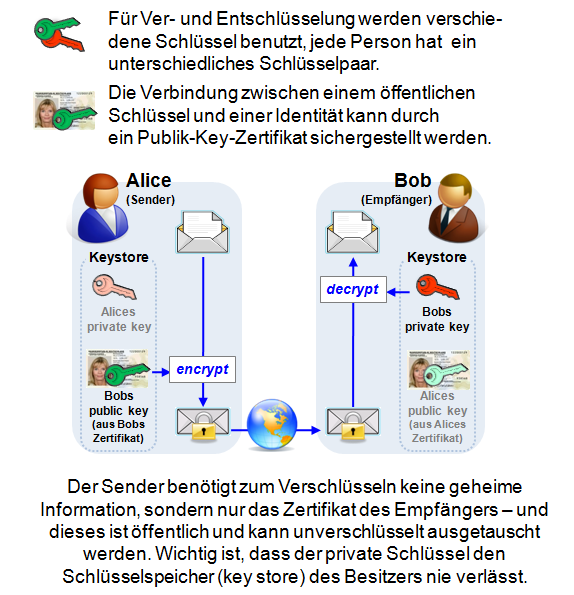
\includegraphics[scale=0.7]{figures/AsymmetricEnc_Figure_Chap1_de.png}
\caption{Asymmetrische oder Public-Key-Verschl�sselung} 
\label{Figure_Asymmetric-Enc_Public-Key-Enc}
\end{center}
\end{figure}

M�chte Alice\index{Alice}%
\footnote{%
  Zur Beschreibung kryptographischer Protokolle werden den Teilnehmern
  oft Namen gegeben (vergleiche \cite[S. 23]{cm:Schneier1996}). 
  Alice und Bob\index{Bob} f�hren alle allgemeinen 2-Personen-Protokolle durch,
  wobei Alice dies initiiert und Bob antwortet.
  Die Angreifer werden als Eve (eavesdropper = passiver Lauscher) und
  Mallory (malicious active attacker = b�swilliger, aktiver Abgreifer)
  bezeichnet.
  }
mit Bob kommunizieren, so sucht sie Bobs �ffentlichen Schl�ssel
und benutzt ihn, um ihre Nachricht an ihn zu
verschl�sseln. Diesen verschl�sselten Text schickt sie dann an Bob,
der mit Hilfe seines geheimen Schl�ssels den Text wieder entschl�s"-seln
kann. Da einzig Bob Kenntnis von seinem geheimen Schl�ssel hat, ist
auch nur er in der Lage, an ihn adressierte Nachrichten zu
entschl�sseln.
Selbst Alice als Absenderin der Nachricht kann aus der von ihr
versandten (verschl�sselten) Nachricht den Klartext nicht wieder
herstellen. Nat�rlich muss sichergestellt sein, dass man aus dem
�ffentlichen Schl�ssel nicht auf den geheimen Schl�ssel schlie�en
kann.\par \vskip + 3pt

% Abbildung evtl. besser hier, wenn Seitenaufteilung ausginge.

Veranschaulichen kann man sich ein solches Verfahren mit einer
Reihe von einbruchssicheren Briefk�sten. Wenn ich eine Nachricht
verfasst habe, so suche ich den Briefkasten\index{Briefkasten} mit dem
Namensschild des Empf�ngers und werfe den Brief dort ein. Danach kann ich die
Nachricht selbst nicht mehr lesen oder ver�ndern, da nur der
legitime Empf�nger im Besitz des Schl�ssels f�r den Briefkasten
ist.\par \vskip + 3pt

Vorteil von asymmetrischen Verfahren ist das einfachere
\index{Schl�sselmanagement} Schl�sselmanagement. Betrachten wir
wieder ein Netz mit $n$ Teilnehmern. Um sicherzustellen, dass
jeder Teilnehmer jederzeit eine verschl�sselte Verbindung zu
jedem anderen Teilnehmer aufbauen kann, muss jeder Teilnehmer ein
Schl�sselpaar besitzen. Man braucht also $2n$ Schl�ssel oder $n$
Schl�sselpaare. Ferner ist im Vorfeld einer �bertragung kein
sicherer Kanal notwendig, da alle Informationen, die zur Aufnahme
einer vertraulichen Kommunikation notwendig sind, offen
�bertragen werden k�nnen. Hier ist lediglich%
\footnote{%
Dass auch dies nicht trivial ist, wird z.B. in Kapitel \ref{nt_Shared-Primes}
erl�utert.
Neben den Anforderungen bei der Schl�sselgenerierung ist zu beachten, dass
inzwischen auch die (Public-Key-)Infrastrukturen selbst Ziel von 
Cyber-Angriffen sind.
}
auf die Unverf�lschtheit (Integrit�t und Authentizit�t)
\index{Authentizit�t} des �ffentlichen Schl�ssels zu achten.
Nachteil: Im Vergleich zu symmetrischen Verfahren sind reine
asymmetrische Verfahren jedoch um ein Vielfaches langsamer.\par \vskip + 3pt

Das bekannteste asymmetrische Verfahren ist der \index{RSA} 
RSA-Algorithmus\index{CrypTool}%
\footnote{%
RSA wird in diesem Skript ab Kapitel \ref{rsabeweis} ausf�hrlich beschrieben.
Die aktuellen Forschungsergebnisse im Umfeld von RSA werden in Kapitel
\ref{SecurityRSA} beschrieben.\\
Das RSA-Kryptosystem kann mit CT1\index{CrypTool 1} �ber das Men� 
{\bf Einzelverfahren \textbackslash{} RSA-Kryptosystem \textbackslash{} 
RSA-Demo} in vielen Variationen nachvollzogen werden.
}%
, der nach seinen Entwicklern Ronald \index{Rivest, Ronald} Rivest, 
Adi \index{Shamir, Adi} Shamir und Leonard \index{Adleman, Leonard} Adleman
benannt wurde. Der RSA-Algorith"-mus wurde 1978 ver�ffentlicht. 
Das Konzept der asymmetrischen Verschl�sselung wurde erstmals
von Whitfield Diffie \index{Diffie, Whitfield}  und 
Martin \index{Hellman, Martin} Hellman in Jahre 1976 vorgestellt. 
Heute spielen auch die Verfahren nach
ElGamal \index{ElGamal, Tahir} eine bedeutende Rolle, vor allem die
\index{Schnorr, C.P.} Schnorr-Varianten im \index{DSA} DSA (Digital
\index{Signatur!digitale}\index{DSA-Signatur}\index{Signatur!DSA}
Signature Algorithm).


% --------------------------------------------------------------------------
\newpage
\section[Hybridverfahren]{Hybridverfahren\footnotemark} 
\footnotetext{%
   In CT1\index{CrypTool 1} finden Sie dieses Verfahren �ber das Men�
   {\bf Ver-/Entschl�sseln \textbackslash{} Hybrid}:
   Dabei k�nnen Sie die einzelnen Schritte und ihre Abh�ngigkeiten mit konkreten
   Zahlen nachvollziehen. Die Variante mit RSA als asymmetrischem Verfahren
   ist graphisch visualisiert; die Variante mit ECC nutzt die Standard-Dialoge.
   In beiden F�llen wird AES als symmetrisches Verfahren eingesetzt.\index{AES}\\
   JCT\index{JCrypTool} bietet Hybrid-Verfahren (z.B. ECIES) in der
   Algorithmen-Perspektive an unter {\bf Algorithms \textbackslash{} Hybrid Ciphers}.
}
\label{CM_Hybrid-procedures}
\index{Hybridverfahren}

Um die Vorteile von symmetrischen und asymmetrischen Techniken gemeinsam 
nutzen zu k�nnen, werden (zur Verschl�sselung) in der Praxis meist 
Hybridverfahren \index{Verschl�sselung!hybrid} verwendet.\par \vskip + 3pt

Hier werden die Mengen-Daten mittels symmetrischer Verfahren
verschl�sselt: Der Schl�ssel ist ein vom Absender zuf�llig\footnote{%
   Die Erzeugung zuf�lliger Zahlen ist ein wichtiger Bestandteil 
   kryptographisch sicherer Verfahren.\\
   Mit CT1\index{CrypTool 1} 
   k�nnen Sie �ber das Men� {\bf Einzelverfahren \textbackslash{}
   Zufallsdaten erzeugen} verschiedene Zufallszahlengeneratoren ausprobieren.
   �ber das Men� {\bf Analyse \textbackslash{} Zufallsanalyse} k�nnen Sie
   verschiedene Testverfahren f�r Zufallsdaten auf bin�re Dokumente
   anwenden.\\
   % CT1 konzentriert sich auf kryptographisch starke
   % {\bf Pseudo}zufallszahlengeneratoren. \glqq Echte\grqq~
   % Zufallsquellen werden nur �ber den Aufruf des Secude-Generators einbezogen.\\
%   CT2 ... xxxxxxxxxxxxxxx\index{ZZZ6c-xxxxxxxxxxxxxxxx-Bsp-Menue aus CT2 ergaenzen}\\
   CT2 ... xxxxxxxxxxxxxxx\index{ZZZ6c-xxxxxxxxxxxxxxxxD} \\
   JCT\index{JCrypTool} bietet {\bf Pseudo}zufallszahlengeneratoren sowohl
   im Men� {\bf Algorithms \textbackslash{} Random Number Generator} der
   Standard-Perspektive als auch in der Algorithmen-Perspektive an.
}\index{Zufall}
generierter geheimer Sitzungsschl�ssel (session key)\index{Session Key},
der nur f�r diese Nachricht verwendet wird.

Anschlie�end wird dieser Sitzungsschl�ssel mit Hilfe des asymmetrischen
Verfahrens verschl�sselt und zusammen mit der Nachricht an den Empf�nger
�bertragen.

Der Empf�nger kann den Sitzungsschl�ssel mit Hilfe seines geheimen
Schl�ssels bestimmen und mit diesem dann die Nachricht entschl�sseln.

Auf diese Weise profitiert man von dem bequemen Schl�sselmanagement\index{Schl�sselmanagement}
asymmetrischer Verfahren (mit �ffentlichem und privatem Schl�ssel), und
man profitiert von der Schnelligkeit symmetrischer Verfahren, um gro�e
Datenmengen zu verschl�sseln (mit den geheimen Schl�sseln).



% --------------------------------------------------------------------------
\newpage
% \vskip +40 pt

\begin{ctsquote}
    Ein altes Sprichwort, angeblich gepr�gt von der
    US National Security Agency (NSA), sagt:\\
    \glqq Angriffe werden immer besser, niemals schlechter.\grqq\\
    ``Attacks always get better; they never get worse.''
\caption[IETF]{IETF\footnotemark}
\end{ctsquote}
\addtocounter{footnote}{0}\footnotetext{%
  \url{http://tools.ietf.org/html/rfc4270}\index{IETF}\index{NSA}
  }

% --------------------------------------------------------------------------
\section[Kryptoanalyse und symmetrische Chiffren f�r Lehrzwecke]{Kryptoanalyse und symmetrische Chiffren f�r Lehrzwecke\footnotemark} 
\footnotetext{%
Ein guter Start in die Kryptoanalyse ist das Buch von Mark Stamp \cite{cm:Stamp2007}.\\
Sehr high-level und nur bezogen auf die Analyse symmetrischer Blockchiffren ist
der Artikel von Bruce Schneier \cite{cm:Schneier2000cm}.\\
Einige der Cipher-Challenges bei \glqq MysteryTwister C3\grqq~
(\url{http://www.mysterytwisterc3.org}) sind ebenfalls gut f�r Lehrzwecke
einsetzbar.\index{MTC3}\index{Challenge}\index{Cipher-Challenge}\index{Krypto-Wettbewerb}
}
\index{Kryptoanalyse}

Verglichen mit den auf der Zahlentheorie beruhenden Public-Key-Verschl�sselungsverfahren wie RSA, ist die Struktur von AES\index{AES} und den meisten anderen modernen symmetrischen Verschl�sse"-lungsverfahren (wie DES, IDEA oder Present) sehr komplex und kann nicht so einfach wie RSA\index{RSA} erkl�rt werden.

Deshalb wurden zu Lehrzwecken vereinfachte Varianten moderner
symmetrischer Verfahren entwickelt, um Einsteigern die M�glichkeit zu geben,
Ver- und Entschl�sselung von Hand zu lernen und ein besseres Verst�ndnis zu
gewinnen, wie die Algorithmen im Detail funktionieren.
Diese vereinfachten Varianten helfen auch, die entsprechenden
Kryptoanalyse-Methoden zu verstehen und anzuwenden.

Eine dieser Varianten ist z.B. S-AES (Simplified-AES) von Prof. Ed Schaefer und
seinen Studenten \cite{cm:Musa-etal2003}.%
\footnote{
    Siehe auch die beiden namensgleichen Artikel
    \glqq Devising a Better Way to Teach and Learn
    the Advanced Encryption Standard\grqq~
    unter den Universit�ts-News bei\\
    - \url{http://math.scu.edu/~eschaefe/getfile.pdf} \\
    - \url{http://www.scu.edu/cas/research/cryptography.cfm}
}
Eine andere Variante ist Mini-AES \cite{cm:Phan2002}
(siehe das Kapitel~\ref{CM_Sage_Mini-AES} \glqq \nameref{CM_Sage_Mini-AES}\grqq)%
\index{DES}\index{DES!SDES}\index{IDEA}:
\begin{itemize}

\item Edward F. Schaefer: {\em A Simplified Data Encryption Standard Algorithm} 
      \cite{cm:Schaefer1996}.

\item Raphael Chung-Wei Phan: {\em Mini Advanced Encryption Standard (Mini-AES):
                                   A Testbed for Cryptanalysis Students} 
      \cite{cm:Phan2002}.

\item Raphael Chung-Wei Phan: {\em Impossible differential cryptanalysis of Mini-AES} 
      \cite{cm:Phan2003}.

\item Mohammad A. Musa, Edward F. Schaefer, Stephen Wedig:
      {\em A simplified AES algorithm and its linear and differential cryptanalyses} 
      \cite{cm:Musa-etal2003}.

\item Nick Hoffman: {\em A SIMPLIFIED IDEA ALGORITHM} 
      \cite{cm:Hoffman2006}.

\item S. Davod. Mansoori, H. Khaleghei Bizaki: 
      {\em On the vulnerability of Simplified AES Algorithm Against Linear Cryptanalysis} 
      \cite{cm:Mansoori-etal2007}.

\end{itemize}



% --------------------------------------------------------------------------
\section{Weitere Informationsquellen}

Neben den anderen Kapiteln in diesem Skript, der umfangreichen Fachliteratur
und vielen Stellen im Internet enth�lt auch die Online-Hilfe aller 
CrypTool-Varianten\index{CrypTool} sehr viele weitere Informationen zu den 
einzelnen symmetrischen und asymmetrischen Verschl�sselungsverfahren.




% ---------------------------------------------------------------------------
% ---------------------------------------------------------------------------
\newpage
\hypertarget{CM_Appendix_SageCode}{}
\section{Anhang: Beispiele mit SageMath}
\label{CM_Sage_samples}
\index{SageMath!Programmbeispiele}

\noindent Der folgende Abschnitt enth�lt SageMath Source-Code, der sich auf den Inhalt des
Kapitels~\ref{Label_Kapitel_1} (\glqq \nameref{Label_Kapitel_1}\grqq) bezieht.

Weitere Details zu in SageMath enthaltenen Kryptoverfahren (z.B. S-DES) finden sich
z.B. in der Diplomarbeit von Minh Van Nguyen \cite{cm:Nguyen2009}.

% ---------------------------------------------------------------------------
\subsection{Mini-AES}
\label{CM_Sage_Mini-AES}
\index{AES!Mini-AES}

Das SageMath-Modul \texttt{crypto/block\_cipher/miniaes.py} enth�lt den Mini-AES, mit
dem Studenten die Funktionsweise moderner Blockchiffren untersuchen k�nnen.

Mini-AES, urspr�nglich vorgestellt von \cite{cm:Phan2002}, ist eine vereinfachte
Variante des Advanced Encryption Standard (AES) f�r Ausbildungszwecke.

Wie man Mini-AES benutzt, ist ausf�hrlich in der SageMath Reference-Page beschrieben:\\
\url{http://www.sagemath.org/doc/reference/sage/crypto/block_cipher/miniaes.html}.

Das folgende SageMath-Code-Beispiel~\ref{cryptomethods:Mini-AES:Sage_example}
ist aus den Release-Notes von SageMath 4.1%
\footnote{
Siehe \url{http://mvngu.wordpress.com/2009/07/12/sage-4-1-released/}
}
und ruft diese Implementierung des Mini-AES auf.

Weiterer Beispiel-Code zum Mini-AES findet sich in
\cite[Kap. 6.5 und Anhang D]{cm:Nguyen2009}.

% Using [fontsize=\footnotesize,fontshape=tt] caused:
%   LaTeX Font Warning: Font shape `T1/cmtt/m/tt' undefined
%   (Font)              using `T1/cmtt/m/n' instead on input line 730.
% so deleted the fontshape parameter.
\begin{sagecode}
\begin{Verbatim}%
[fontsize=\footnotesize]
# We can encrypt a plaintext using Mini-AES as follows:
sage: from sage.crypto.block_cipher.miniaes import MiniAES
sage: maes = MiniAES()
sage: K = FiniteField(16, "x")
sage: MS = MatrixSpace(K, 2, 2)
sage: P = MS([K("x^3 + x"), K("x^2 + 1"), K("x^2 + x"), K("x^3 + x^2")]); P

[  x^3 + x   x^2 + 1]
[  x^2 + x x^3 + x^2]
sage: key = MS([K("x^3 + x^2"), K("x^3 + x"), K("x^3 + x^2 + x"), K("x^2 + x + 1")]); key

[    x^3 + x^2       x^3 + x]
[x^3 + x^2 + x   x^2 + x + 1]
sage: C = maes.encrypt(P, key); C

[            x       x^2 + x]
[x^3 + x^2 + x       x^3 + x]

# Here is the decryption process:
sage: plaintxt = maes.decrypt(C, key)
sage: plaintxt == P
True

# We can also work directly with binary strings:
sage: from sage.crypto.block_cipher.miniaes import MiniAES
sage: maes = MiniAES()
sage: bin = BinaryStrings()
sage: key = bin.encoding("KE"); key
0100101101000101
sage: P = bin.encoding("Encrypt this secret message!")
sage: C = maes(P, key, algorithm="encrypt")
sage: plaintxt = maes(C, key, algorithm="decrypt")
sage: plaintxt == P
True

# Or work with integers n such that 0 <= n <= 15:
sage: from sage.crypto.block_cipher.miniaes import MiniAES
sage: maes = MiniAES()
sage: P = [n for n in xrange(16)]; P
[0, 1, 2, 3, 4, 5, 6, 7, 8, 9, 10, 11, 12, 13, 14, 15]
sage: key = [2, 3, 11, 0]; key
[2, 3, 11, 0]
sage: P = maes.integer_to_binary(P)
sage: key = maes.integer_to_binary(key)
sage: C = maes(P, key, algorithm="encrypt")
sage: plaintxt = maes(C, key, algorithm="decrypt")
sage: plaintxt == P
True
\end{Verbatim}
\caption{Ver- und Entschl�sselung mit dem Mini-AES}
\label{cryptomethods:Mini-AES:Sage_example}
\end{sagecode}



% ---------------------------------------------------------------------------
\subsection{Weitere symmetrische Krypto-Algorithmen in SageMath}
\label{CM_Sage_SymCryptoAlg}

Die SageMath-Referenz v5.4.1%
%
\footnote{
Siehe \url{http://www.sagemath.org/doc/reference/sage/crypto/}
}
f�hrt als weitere Chiffren auf:\\ 
- Linear feedback shift register (LFSR),\\
- ShrinkingGeneratorCryptosystem,\\
- Blum-Blum-Shub (BBS): Pseudo-Zufallsbit-Generator,\\
- Gitter-bezogene Funktionen.




% --------------------------------------------------------------------------
%xxxxxxxxxxx
%\bibitem[x]{cm:x}  \index{x}
%        x, \\
%        {\em x}, 
%       x x.
%xxxxxxxxxxx
\newpage
\begin{thebibliography}{99999}
\addcontentsline{toc}{section}{Literaturverzeichnis}

\bibitem[Biryukov2009]{cm:Biryukov2009} \index{Biryukov 2009}
	Alex Biryukov, Dmitry Khovratovich,\\
	{\em Related-key Cryptanalysis of the Full AES-192 and AES-256},
	2009.\\
	\url{http://eprint.iacr.org/2009/317}

\bibitem[Coppersmith2002]{cm:Coppersmith2002}  \index{Coppersmith 2002}
       Don Coppersmith, \\
       {\em Re: Impact of Courtois and Pieprzyk results},\\ 
       19.09.2002, in den \glqq AES Discussion Groups\grqq~unter\\
       \url{http://aes.nist.gov/aes/}

\bibitem[Courtois2002]{cm:Courtois2002}  \index{Courtois 2002}
       Nicolas Courtois, Josef Pieprzyk, \\
       {\em Cryptanalysis of Block Ciphers with Overdefined Systems
            of Equations}, \\
       received 10 Apr 2002, last revised 9 Nov 2002.\\
       Eine davon verschiedene~\glqq compact version\grqq~des ersten
       XSL-Angriffs wurde auf der Asiacrypt im Dezember 2002 ver�ffentlicht.\\
       \url{http://eprint.iacr.org/2002/044}

\bibitem[Ferguson2001]{cm:Ferguson2001}  \index{Ferguson 2001}
       Niels Ferguson, Richard Schroeppel, Doug Whiting, \\
       {\em A simple algebraic representation of Rijndael}, 
       Draft 1. Mai 2001. \\
       \url{http://www.xs4all.nl/~vorpal/pubs/rdalgeq.html}

\bibitem[Haan2008]{cm:Haan2008} \index{Haan 2008} 
       Kristian Laurent Haan, \\
       {\em Advanced Encryption Standard (AES)},
       2008. \\
       \url{http://www.codeplanet.eu/tutorials/cpp/51-advanced-encryption-standard.html}

\bibitem[Hoffman2006]{cm:Hoffman2006} \index{Hoffman 2006} 
       Nick Hoffman, \\
       {\em A SIMPLIFIED IDEA ALGORITHM},
       2006. \\
       \url{http://www.nku.edu/~christensen/simplified%20IDEA%20algorithm.pdf}

\bibitem[Lucks-DuD2002]{cm:Lucks-DuD2002}  \index{Lucks 2002}
       Stefan Lucks, R�diger Weis, \\
       {\em Neue Ergebnisse zur Sicherheit des Verschl�sselungsstandards AES},\\
       in DuD 12/2002.

\bibitem[Mansoori-etal2007]{cm:Mansoori-etal2007} \index{Mansoori, Bizaki 2007} 
       S. Davod. Mansoori, H. Khaleghei Bizaki, \\
       {\em On the vulnerability of Simplified AES Algorithm Against Linear
       Cryptanalysis}, \\
       In: IJCSNS International Journal of Computer Science and Network Security,
       Vol. 7 No. 7, Juli 2007, Seite~257-263. \\
       Siehe auch:\\
       \url{http://paper.ijcsns.org/07_book/200707/20070735.pdf}

\bibitem[Massacci2000]{cm: Massacci2000} \index{Massacci 2000}
       Fabio Massacci, Laura Marraro \\
       {\em Logical cryptanalysis as a SAT problem: Encoding and analysis},\\
       In: Journal of Automated Reasoning Security,
       Vol. 24, 2000, Seite~165-203.

\bibitem[Menezes2001]{cm:Menezes2001} \index{Menezes 2001}
       Alfred J. Menezes, Paul C. van Oorschot, Scott A. Vanstone \\
       {\em Handbook of Applied Cryptography}, 
       CRC Press 1997, 5th printing 2001.\\
       \url{http://www.cacr.math.uwaterloo.ca/hac/} (Errata last update 24.07.2011)

\bibitem[Mironov2006]{cm: Mironov2006} \index{Mironov 2006}
       Ilya Mironov, Lintao Zhang \\
       {\em Applications of SAT Solvers to Cryptanalysis of Hash Functions}, 
       Springer 2006.

\bibitem[Musa-etal2003]{cm:Musa-etal2003} \index{Musa, Schaefer, Wedig 2003} 
       Mohammad A. Musa, Edward F. Schaefer, Stephen Wedig, \\
       {\em A simplified AES algorithm and its linear and differential cryptanalyses}, \\
       In: Cryptologia 17 (2), April 2003, Seite~148-177.\\
       Siehe auch:\\
%       \url{http://findarticles.com/p/articles/mi_qa3926/is_200304/ai_n9181658}\\
       \url{http://www.rose-hulman.edu/~holden/Preprints/s-aes.pdf}\\
       \url{http://math.scu.edu/~eschaefe/}   Ed Schaefer's Homepage

\bibitem[Nguyen2009]{cm:Nguyen2009} \index{Nguyen 2009} 
       Minh Van Nguyen, \\
       {\em Exploring Cryptography Using the Sage Computer Algebra System}, \\
       Victoria University, 2009. \\
       Siehe SageMath publications \url{http://www.sagemath.org/library-publications.html},\\
       \url{http://www.sagemath.org/files/thesis/nguyen-thesis-2009.pdf},\\
       \url{http://sites.google.com/site/nguyenminh2/honours-thesis-2009.pdf}

\bibitem[Nichols1996]{cm:Nichols1996} \index{Nichols 1996} 
       Randall K. Nichols, \\
       {\em Classical Cryptography Course, Volume 1 and 2}, \\
       Aegean Park Press 1996; \\
       oder in 12 Lektionen online unter: \\
       \url{http://www.fortunecity.com/skyscraper/coding/379/lesson1.htm}

\bibitem[Oppliger2011]{cm:Oppliger2011} \index{Oppliger 2011}
       Rolf Oppliger \\
       {\em Contemporary Cryptography, Second Edition},
       Artech House, 2011. \\
       \url{http://books.esecurity.ch/cryptography2e.html}.

\bibitem[Phan2002]{cm:Phan2002} \index{Phan 2002} 
       Raphael Chung-Wei Phan, \\
       {\em Mini Advanced Encryption Standard (Mini-AES): A Testbed for
            Cryptanalysis Students}, \\
       In: Cryptologia 26 (4), 2002, Seite~283-306.

\bibitem[Phan2003]{cm:Phan2003} \index{Phan 2003} 
       Raphael Chung-Wei Phan, \\
       {\em Impossible differential cryptanalysis of Mini-AES}, \\
       In: Cryptologia, Oct 2003.\\
       \url{http://findarticles.com/p/articles/mi_qa3926/is_200310/ai_n9311721/}

\bibitem[Robshaw2002a]{cm:Robshaw2002a}  \index{Robshaw 2002}
       S.P. Murphy, M.J.B. Robshaw, \\
       {\em Essential Algebraic Structure within the AES},\\
       5. Juni 2002, auf der Crypto 2002.  \\
       \url{http://www.isg.rhul.ac.uk/~mrobshaw/rijndael/rijndael.html}

\bibitem[Robshaw2002b]{cm:Robshaw2002b}  \index{Robshaw 2002}
       S.P. Murphy, M.J.B. Robshaw, \\
       {\em Comments on the Security of the AES and the XSL Technique},\\
       26. September 2002. \\
       \url{http://www.isg.rhul.ac.uk/~mrobshaw/rijndael/rijndael.html}

\bibitem[Schaefer1996]{cm:Schaefer1996} \index{Schaefer 1996} 
       Edward F. Schaefer, \\
       {\em A Simplified Data Encryption Standard Algorithm}, \\
       In: Cryptologia 20 (1), 1996, Seite~77-84.

\bibitem[Schmeh2016]{cm:Schmeh2016}  \index{Schmeh 2016}
       Klaus Schmeh, \\
       {\em Kryptografie -- Verfahren, Protokolle, Infrastrukturen},\\ 
       dpunkt.verlag, 6. aktualisierte und erweiterte Auflage 2016. \\
       Sehr gut lesbares, aktuelles und umfangreiches Buch �ber Kryptographie. 
       Geht auch auf praktische Probleme, wie Standardisierung oder 
       real existierende Software, ein.

\bibitem[Schneier1996]{cm:Schneier1996} \index{Schneier 1996} 
       Bruce Schneier, \\
       {\em Applied Cryptography, Protocols, Algorithms, and Source Code in C}, \\
       Wiley 1994, 2nd edition 1996.

\bibitem[Schneier2000]{cm:Schneier2000cm} \index{Schneier 2000} 
       Bruce Schneier, \\
       {\em A Self-Study Course in Block-Cipher Cryptanalysis}, \\
       In: Cryptologia, v.24, Jan 2000, Seite~18-34.\\
       \url{www.schneier.com/paper-self-study.pdf}

\bibitem[Stallings2006]{cm:Stallings2006} \index{Stallings 2006} 
       William Stallings, \\
       {\em Cryptography and Network Security}, \\
       Prentice Hall 2006.\\
       \url{http://williamstallings.com/}

\bibitem[Stamp2007]{cm:Stamp2007} \index{Stamp 2007} 
       Mark Stamp, Richard M. Low, \\
       {\em Applied Cryptanalysis: Breaking Ciphers in the Real World}, \\
       Wiley-IEEE Press 2007. \\
       \url{http://cs.sjsu.edu/faculty/stamp/crypto/}

\bibitem[Swenson2008]{cm:Swenson2008} \index{Swenson 2008} 
       Christopher Swenson, \\
       {\em Modern Cryptanalysis: Techniques for Advanced Code Breaking}, \\
       Wiley 2008.

\bibitem[Wobst-iX2002]{cm:Wobst-iX2002}  \index{Wobst 2002}
       Reinhard Wobst, \\
       {\em Angekratzt -- Kryptoanalyse von AES schreitet voran},\\
       in iX 12/2002, \\
       und der Leserbrief dazu von Johannes Merkle in der iX 2/2003.

\end{thebibliography}


% --------------------------------------------------------------------------
\newpage
\chapter*{Web-Links}\addcontentsline{toc}{section}{Web-Links}

\begin{enumerate}

%  \item[] \href{http://www.cryptosystem.net/aes}
%       {\texttt{http://www.cryptosystem.net/aes}} 
%  per item[] werden sie NICHT durchnummeriert !
  \hypertarget{CM_HT_Weblink_Rijndael-Cryptosystem}{}
  \item Das AES-/Rijndael-Kryptosystem \\
        \url{http://www.cryptosystem.net/aes}

\item \glqq AES Discussion Groups\grqq~beim NIST \\ %%% \grqq nach \item braucht die Tilde, aber kein weiteres Blank. Sonst reicht ein Blank, wenn ein weiteres Wort danach folgt (es reicht auch sonst nicht, wenn danach der Zeilenumbruch).
	\url{http://csrc.nist.gov/archive/aes/}

  \item distributed.net:~\glqq RC5-64 has been solved\grqq \\
        \url{http://www.distributed.net/Pressroom_press-rc5-64}

  \item RSA: ~\glqq The RSA Secret Key Challenge\grqq \\
        \url{http://www.rsa.com/rsalabs/node.asp?id=2100}

  \item RSA: ~\glqq DES Challenge\grqq \\
        \url{http://www.rsa.com/rsalabs/node.asp?id=2108}

  \item Weiterf�hrende Links auf der CrypTool-Homepage \\
        \url{http://www.cryptool.org}
	       
\end{enumerate}

Alle Links wurden am 12.12.2012 �berpr�ft.



% Local Variables:
% TeX-master: "../script-de.tex"
% End:

% $Id: paper_and_pencil.tex 3706 2016-03-18 10:29:15Z rainer $
% ..............................................................................
%                V E R S C H L U E S S E L U N G S V E R F A H R E N
%
% Writing rule: Chapter header with all nouns/verbs-words capitalized,
%               All other headers in the normal lower/upper case manner
%               like sentences (without a dot at the end).
% Writing rule: Use American English instead of British English consistently.
%
% ~~~~~~~~~~~~~~~~~~~~~~~~~~~~~~~~~~~~~~~~~~~~~~~~~~~~~~~~~~~~~~~~~~~~~~~~~~~~~~
%------------------------------------------------------------------------------
% First Editor: Christine St�tzel, April 2004
% Update and corrections: B. Esslinger, June 2005
% Update and corrections: B. Esslinger, June 2005
% Update B. Esslinger and Minh Van Nguyen, November 2009 
% Update B. Esslinger, June 2010 
% Update B. Esslinger, Jan. 2013 
%------------------------------------------------------------------------------

% ``primenet''
\newpage
\hypertarget{Kapitel_PaperandPencil}{}

\chapter{Paper and Pencil Encryption Methods}
\label{Kapitel_PaperandPencil}
(Christine St\"otzel, April 2004; Updates: B.+C. Esslinger, June 2005;
 Updates Minh Van Nguyen and B. Esslinger, Nov. 2009, June 2010, May 2013)
\index{paper and pencil methods}
\index{encryption!classic}
\index{cryptography!classic}

\begin{ctsquote}
Few persons can be made to believe that it is not quite an easy thing
to invent a method of secret writing which shall baffle investigation.
Yet it may be roundly asserted that human ingenuity cannot concoct a
cipher which human ingenuity cannot resolve.
\caption[Edgar Allan Poe]{Edgar Allan Poe: A Few Words on Secret Writing, 1841}\index{Poe, Edgar Allan}
\end{ctsquote}

The following chapter provides a broad overview of paper and pencil 
methods\footnote{%
The footnotes of this chapter describe how these methods can be
performed using the offline programs CrypTool 1 ({\bf CT1})\index{CT1},
CrypTool 2 ({\bf CT2})\index{CT2} and JCrypTool ({\bf JCT})\index{JCT}.
See the appendices
\ref{s:appendix-menu-overview-CT1},
\ref{s:appendix-template-overview-CT2}, and
\ref{s:appendix-function-overview-JCT}.\\
Many of the methods can also per performed within a browser, e.g. on the
website CrypTool-Online ({\bf CTO}) (\url{http://www.cryptool-online.org})\index{CTO}. See the appendix \ref{s:appendix-function-overview-CTO}.\\
Additionally the last sub chapter (\ref{PaP_Sage_samples})
contains example code for the computer-algebra system {\bf SageMath}\index{SageMath}.
                 }
each with references to deeper information.
All techniques that people can apply manually to en- and decipher a message are 
embraced by this term. These methods were and still are especially popular with
secret services, as a writing pad and a pencil -- in contrast to electronic
aids -- are totally unsuspicious.

The first paper and pencil methods already arose about 3000 years ago, but new
procedures were developed during the past century, too. All paper and pencil 
methods are a matter of symmetric methods\index{encryption!symmetric}. 
Even the earliest encryption algorithms use the basic principles such as 
transposition, substitution, block construction and their combinations. 
Hence it is worthwhile to closely consider this ``ancient'' methods especially
under didactic aspects.

Methods to be successful and wide-spread had to fulfill some attributes
which are equally required for modern algorithms:
\begin{itemize}
\item Exhaustive description, almost standardization (including special cases,
      padding, etc.).
\item Good balance between security and usability 
      (because methods being too complicated were error-prone or
      unacceptably slow).
\end{itemize}


\newpage
%------------------------------------------------------------------------------
\section{Transposition ciphers}
\label{PaP_transposition_ciphers}
\index{transposition}

Encrypting a message by means of transposition\index{transposition} does not 
change the original characters of this message, only their order is modified
(transposition = exchange).\footnote{%
Sometimes, the name permutation\index{permutation} is used to describe how
characters, groups of characters or columns of the plaintext are exchanged, e.g.
$(1, 2, 3, 4, 5) \Leftrightarrow (3, 4, 2, 1, 5)$.
}

%------------------------------------------------------------------------------
\subsection{Introductory samples of different transposition ciphers}
\label{introsamplesTranspositionCiphers}

\begin{itemize}

\item {\bf Rail fence cipher}\footnote{%
   This method can directly be found in CT1\index{CrypTool 1} at the menu item
   {\bf Encrypt/Decrypt \textbackslash{} Symmetric (classic) \textbackslash{}
   Scytale / Rail Fence}.
   You can simulate this method also under the menu {\bf Encrypt/Decrypt
   \textbackslash{} Symmetric (classic) \textbackslash{} Permutation}:
   For a Rail Fence with 2 lines use as key ``B,A'' and accept the default
   settings (only one permutation, where your input is done line-by-line and
   the output is taken column-by-column). 
   Using the key ``A,B'' would start the zigzag pattern below in the
   way, that the first letter is written into the first line instead of the
   second line.}
   \cite{pp:Singh1999}\index{rail fence cipher}:
   The characters of a message are alternately written in two (or more) lines,
   creating a zigzag pattern. The resulting ciphertext is read out 
   line by line.\\
   This is more a children's method.

   See table \ref{PaP_RailFence_table-reference}.

   Plaintext\footnote{\index{agreement}: If the alphabet only uses 26 letters,
   we write from now onwards the plaintext in small letters and the ciphertext
   in capital letters.}:
   an example of transposition

   \begin{table}[ht]
   \begin{center}
   \begin{tabular}{r@{\:}r@{\:}r@{\:}r@{\:}r@{\:}r@{\:}r@{\:}r@{\:}r@{\:}r@{\:}r@{\:}r@{\:}r@{\:}r@{\:}r@{\:}r@{\:}r@{\:}r@{\:}r@{\:}r@{\:}r@{\:}r@{\:}r@{\:}r@{\:}}
	  & n &   & x &   & m &   & l &   & o &   & t &   & a &   & s &   & o &   & i &   & i &   & n \\
	a &   & e &   & a &   & p &   & e &   & f &   & r &   & n &   & p &   & s &   & t &   & o &   \\
   \end{tabular}
   \caption{Rail Fence cipher}
   \label{PaP_RailFence_table-reference}
   \end{center} 
   \end{table}

   Ciphertext\footnote{The letters of the plaintext are -- as used 
   historically -- grouped within blocks of 5 letters. It does not matter
   if the (constant) block length is different or no blank is inserted.}%
   : NXMLO TASOI INAEA PEFRN PSTO\\


\item {\bf Scytale}\footnote{%
    This method can directly be found in CT1\index{CrypTool 1} at the menu item
    {\bf Encrypt/Decrypt \textbackslash{} Symmetric (classic) \textbackslash{}
    Scytale / Rail Fence}.
    As this method is a special case of a simple columnar transposition, you also can
    simulate it in CT1\index{CrypTool 1} under the 
    menu {\bf Encrypt/Decrypt \textbackslash{} Symmetric (classic) \textbackslash{} 
    Permutation}: For the Scytale within the dialog box only the first 
    permutation is used. If the wood has e.g.\ 4 angles use as key ``1,2,3,4''.
    This is equivalent to write the text horizontally in blocks of 4 letters 
    in a matrix and to read it out vertically . 
    Because the key is in an in ascending order, the Scytale is denoted as
    an identical permutation. And because writing and read-out is done only
    once it is a simple (and no double) permutation.\\
    In CT2\index{CrypTool 2} you can find the Scytale within the templates
    {\bf Cryptography \textbackslash{} Classical}).
   }
   \cite{pp:Singh1999}\index{Scytale}%
   : 
   This method was probably used since 600 B.C. -- a description
   of how it operated is not known from before Plutarch (50-120 B.C.).\\
   A long strip of paper is wrapped around a wooden cylinder and then the 
   message is written along the length of this strip. The ciphertext is 
   produced by unwinding the strip.


\item {\bf Grille cipher} \cite{pp:Goebel2003}: Both parties use identical
   stencils. 
   Line by line, their holes are filled with plaintext that is read out 
   column by column to produce the ciphertext. If there is plaintext left, 
   the procedure is repeated.\footnote{%
   This method cannot be simulated with a pure column transposition.}


   \hypertarget{turning-grille cipher}{}
\item {\bf Turning grille} \cite{pp:Savard1999}%
   \index{turning grille}: 
   The German army used turning grilles during WW1.\footnote{%
      The turning grille was already invented in 1881 by Eduard Fleissner von
      Wostrowitz.\\
      A good visualization can be found under www.turning-grille.com.\\
      In JCT\index{JCrypTool} you can find it in the default perspective
      via the menu item {\bf Visuals \textbackslash{} Grille}.
   } 
   A square grille serves as a stencil, a quarter of its fields being holes.
   The first part of the message is written on a piece of paper through	these
   holes, then the grille is rotated by 90 degrees and the user can
   write down the second part of the message, etc. But this method does only
   work, if the holes are chosen carefully: Every field has to be used, and
   no field may be used twice, either. The ciphertext is read out line by
   line.

   In the example for a turning grille in table \ref{PaP_88Fleissner_table-reference}
   you can write 4 times 16 characters of the plaintext on a piece of paper:
   \begin{table}[ht]
   \begin{center}
   \begin{tabular}{|cccc|cccc|}
   \hline 	
	O & - & - & - & - & O & - & - \\
	- & - & - & O & O & - & - & O \\
	- & - & - & O & - & - & O & - \\
	- & - & O & - & - & - & - & - \\
   \hline 	
	- & - & - & - & O & - & - & - \\
	O & - & O & - & - & - & O & - \\
	- & O & - & - & - & - & - & O \\
	- & - & - & O & O & - & - & - \\
   \hline
   \end{tabular}  
   \caption{8x8 turning grille} 
   \label{PaP_88Fleissner_table-reference}
   \end{center}   
   \end{table}

\end{itemize}


%------------------------------------------------------------------------------
% {\bf Column and row transposition}
\subsection[Column and row transposition ciphers]
    {Column and row transposition\footnotemark}
    \footnotetext{%
Most of the following methods can be simulated in CT1\index{CrypTool 1} 
under the menu {\bf Encrypt/Decrypt \textbackslash{} Symmetric (classic) 
\textbackslash{} Permutation}.}

\begin{itemize}

\item {\bf Simple columnar transposition} \cite{pp:Savard1999}: First of all, 
   a keyword is chosen, that is written above the columns of a table. This
   table is filled with the text to be encrypted line by line. Then the 
   columns are rearranged by sorting the letters of the keyword alphabetically.
   Afterwards the columns are read out from left to right to build the 
   ciphertext.\footnote{%
   Using CT1: Choose a key for the 1st permutation, input line by line, 
   permute and output column by column.}

   See table \ref{PaP_SimpColTransp_table-reference}.

   Plaintext: an example of transposition

\begin{table}[ht]
\begin{center}
\begin{tabular}{|c|c|c|}
\hline 	
	K & E & Y \\
\hline
	a & n & e \\
	x & a & m \\
	p & l & e \\
	o & f & t \\
	r & a & n \\
	s & p & o \\
	s & i & t \\
	i & o & n \\
\hline
\end{tabular}
\caption{Simple columnar transposition}
\label{PaP_SimpColTransp_table-reference}
\end{center} 
\end{table}

   Transposition key: K=2; E=1; Y=3. \\
   Ciphertext: NALFA PIOAX PORSS IEMET NOTN\\


\item {\bf AMSCO cipher} \cite{pp:ACA2002}\index{AMSCO}: The characters of the
   plaintext are written in alternating groups of one respectively two letters
   into a grille. Then the columns are swapped and the text can be read out.


\item {\bf Double column transposition} \cite{pp:Savard1999}
   \index{double column transposition}: 
   Double columnar transposition
   was frequently used during WW2 and during the Cold War. Two simple columnar
   transpositions with different keys are executed successively.\footnote{%
   Using CT1: Choose a key for the 1st permutation, input line by line, 
   permute and output column by column. Then choose a (different) key for the
   2nd permutation, input line by line, permute and output column by column.}\\
   If the keys are different and long enough (at least each 20 characters),
   then this is even for today's computer a real challenge.\footnote{%
     MTC3\index{MTC3} offers an according level-X challenge called
     ``Double Columnar Transposition'':\\
     \url{http://www.mysterytwisterc3.org/en/challenges/level-x/double-column-transposition}
   }



\item {\bf Column transposition, General Luigi Sacco} \cite{pp:Savard1999}: The 
   columns of a table are numbered according to the letters of the keyword. 
   The plaintext is entered line by line, in the first line up to column 
   number one, in the second line up to column number two, etc. 
   Again, the ciphertext is read out in columns.

   See table \ref{PaP_LuigiSacco_table-reference}.

   Plaintext: an example of transposition

\begin{table}[ht]
\begin{center}
\begin{tabular}{|c|c|c|c|c|c|}
\hline 	
	C & O & L & U & M & N\\
	1 & 5 & 2 & 6 & 3 & 4\\
\hline
	a &   &   &   &   &  \\
	n & e & x &   &   &  \\
	a & m & p & l & e &  \\
	o & f & t & r & a & n\\
	s & p &   &   &   &  \\
	o & s & i & t &   &  \\
	i & o & n &   &   &  \\
\hline
\end{tabular}
\caption{Columnar transposition (General Luigi Sacco)}
\label{PaP_LuigiSacco_table-reference}
\end{center} 
\end{table}

   Ciphertext: ANAOS OIEMF PSOXP TINLR TEAN\\


\item {\bf Column transposition, French army in WW1} 
   \cite{pp:Savard1999}: 
   After executing a simple columnar transposition, diagonal rows are read out.


\item {\bf Row transposition} \cite{pp:Savard1999}: The plaintext is divided 
   into blocks of equal length and a keyword is chosen.
   Now the letters of the keyword are numbered and permutation is done only
   within each block according to this numbering.\footnote{%
   Using CT1: Choose a key for 1st permutation, input line by line, 
   permute column by column and output line by line.}

\end{itemize}



%------------------------------------------------------------------------------
\subsection{Further transposition algorithm ciphers}

\begin{itemize}

\item {\bf Geometric figures} \cite{pp:Goebel2003}: Write the message into a
   grille following one pattern and read it out using another.

\item {\bf Union Route Cipher} \cite{pp:Goebel2003}: The Union Route Cipher
   derives from Civil War. This method does not rearrange letters of a given
   plaintext, but whole words. Particularly sensitive names and terms are
   substituted by codewords which are recorded in codebooks together with
   the existing routes.
   A route determines the size of a grille and the pattern that is used to 
   read out the ciphertext. In addition, a number of filler words is defined.

\item {\bf Nihilist Transposition} \cite{pp:ACA2002}\index{Nihilist transposition}: 
   Insert the plaintext into 
   a square grille and write the same keyword above the columns and next to
   the lines. As this keyword is sorted alphabetically, the contents of the
   grille are rearranged, too. Read out the ciphertext line by line.

   See table \ref{PaP_NihilistTransp_table-reference}.
	
   Plaintext: an example of transposition

\begin{table}[ht]
\begin{center}
\begin{tabular}{|c|ccccc||cc|ccccc|}
\hline 	
	  & W & O & R & D & S &   &   & D & O & R & S & W\\
\hline
	W & a & n & e & x & a &   & D & s & p & o & i & s\\
	O & m & p & l & e & o &   & O & e & p & l & o & m\\
	R & f & t & r & a & n &   & R & a & t & r & n & f\\
	D & s & p & o & s & i &   & S & n & i & o & - & t\\
	S & t & i & o & n & - &   & W & x & n & e & a & a\\
\hline
\end{tabular}  
\caption[Nihilist transposition]{Nihilist transposition\footnotemark}
   \label{PaP_NihilistTransp_table-reference}
\end{center} 
\end{table}

   Ciphertext: SPOIS EPLOM ATRNF NIOTX NEAA\\
   \footnotetext{%
   After filling the matrix with the plaintext you get the left block.
   After switching rows and columns you get the right block}


%\newpage % Damit die Tables immer direkt nach dem zugeh�rigen Item. 
\item {\bf Cadenus cipher} \cite{pp:ACA2002}\index{Cadenus cipher}: Cadenus is
   a form of columnar transposition that uses two keywords.\\
   The 1st keyword is used to swap columns.\\
   The 2nd keyword is used to define the initial letter of each column:
   this 2nd keyword is a permutation of the used alphabet. This permutation
   is written on the left of the first column.
   Afterwards, each column is moved (wrap-around) so that it begins with the
   letter, which is in the same line as the key letter of the first 
   keyword within the second keyword. Ciphertext is read out line by line.

   See table \ref{PaP_Cadenus-table-reference}.
		
   Plaintext: cadenus is a form of columnar transposition using a keyword

\begin{table}[ht]
\begin{center}
\begin{tabular}{|c|ccc|ccc|ccc|}
\hline 	
	  & K & {\bf E} & Y & {\bf E} & K & Y & {\bf E} & K & Y\\
\hline
	A & c & a & d & a & c & d & {\bf s} & a & a\\
	D & e & n & u & n & e & u & s & r & p\\
	X & s & i & s & i & s & s & i & f & i\\
	K & a & f & o & f & {\bf a} & o & u & l & o\\
	C & r & m & o & m & r & o & n & n & s\\
	W & f & c & o & c & f & o & k & t & g\\
	N & l & u & m & u & l & m & w & n & e\\
	S & n & a & r & a & n & r & d & o & o\\
	Y & t & r & a & r & t & {\bf a} & a & t & d\\
	{\bf E} & n & {\bf s} & p & {\bf s} & n & p & n & n & u\\
	D & o & s & i & s & o & i & i & i & s\\
	T & t & i & o & i & t & o & f & a & o\\	
	U & n & u & s & u & n & s & m & y & o\\
	B & i & n & g & n & i & g & c & r & o\\
	R & a & k & e & k & a & e & u & c & m\\
	G & y & w & o & w & y & o & a & e & r\\
	H & r & d & - & d & r & - & r & s & -\\
\hline
\end{tabular}  
\caption[Cadenus]{Cadenus cipher\footnotemark}
\label{PaP_Cadenus-table-reference}
\end{center} 
\end{table}%

   Ciphertext:\\
   SAASR PIFIU LONNS KTGWN EDOOA TDNNU IISFA OMYOC ROUCM AERRS\\
   \footnotetext{%
   Within the 2nd block of three chars those chars are printed bold which
   are at the top of the 3rd block after applying the 2nd key word.}

\end{itemize}



%------------------------------------------------------------------------------
\section{Substitution ciphers}
\label{PaP_substitution_ciphers}
\index{substitution}


%------------------------------------------------------------------------------
\subsection{Monoalphabetic substitution ciphers}
Monoalphabetic substitution\index{substitution!monoalphabetic} assigns one 
character of the ciphertext alphabet to each plaintext character. This mapping
remains unchanged during the whole process of encryption.
\label{monoalphabeticSubstitutionCiphers}

\begin{itemize}

\item {\bf General monoalphabetic substitution / Random letter 
   pairs\footnotemark}
   \footnotetext{%
    This cipher can be simulated in CT1\index{CrypTool 1} 
    under the menu {\bf Encrypt/Decrypt \textbackslash{} Symmetric (classic) 
    \textbackslash{} Substitution / Atbash}.\\
    In CT2\index{CrypTool 2} you can find these methods within the templates
    {\bf Cryptography \textbackslash{} Classical}).
   } 
   \cite{pp:Singh1999}:
   The substitution occurs by a given assignment of single letters.

\item {\bf Atbash cipher\footnotemark}
   \footnotetext{%
   This cipher can be simulated in CT1\index{CrypTool 1} 
   under the menu {\bf Encrypt/Decrypt \textbackslash{} Symmetric (classic) 
   \textbackslash{} Substitution / Atbash}.}  
   \cite{pp:Singh1999}\index{Atbash cipher}: Replace the first letter of the 
   alphabet by the last letter of the alphabet, the second one by the last 
   but one, etc.

\item {\bf Shift cipher, for example Caesar cipher}\footnote{In CT1\index{CrypTool 1}
   this method  can be found at three different places in the menu tree:\\
   - {\bf Encrypt/Decrypt \textbackslash{} Symmetric (classic) \textbackslash{} 
      Caesar / ROT13}\\
   - {\bf Analysis \textbackslash{} Symmetric Encryption (classic)
     \textbackslash{} Ciphertext only \textbackslash{} Caesar} \\
   - {\bf Indiv. Procedures \textbackslash{} Visualization of Algorithms 
     \textbackslash{} Caesar}. } 
   \cite{pp:Singh1999}\index{Caesar cipher}%
   : Plaintext alphabet and ciphertext alphabet are shifted against each 
   other by a determined number of letters. Using the Caesar cipher means 
   shifting letters about three positions.

    Plaintext:  \texttt{		three positions to the right}

    Ciphertext: \texttt{		WKUHH SRVLWLRQV WR WKH ULJKW}


\item {\bf Affine cipher}\footnote{
   Some according SageMath samples are implemented at \ref{PaP_affine_cipher_sage-sample}.
   }%
   \index{affine cipher}: This is a generalization of
   the shift cipher. A plaintext character is first substituted by another
   character and then the result is encrypted using the shift cipher.
   The name ``affine cipher'' was chosen because its encryption and
   decryption can be described as affine or linear function.

\item {\bf Substitution with symbols} \cite{pp:Singh1999}, for instance the 
   so-called ``freemason cipher'': Each letter is replaced with a symbol.

\item {\bf Variants}: Fill characters, intentional mistakes \cite{pp:Singh1999}.

\item {\bf Nihilist substitution}\footnote{An animation of this Nihilist method
   can be found in CT1\index{CrypTool 1} at the menu item
     {\bf Indiv. Procedures \textbackslash{} Visualization of Algorithms 
     \textbackslash{} Nihilist}. }
   \cite{pp:ACA2002}\index{Nihilist substitution}: 
   Insert the alphabet into a 5x5-matrix to assign each letter the number built 
   from row and column number.  
   A keyword is chosen and placed above the columns of a second matrix (grille). 
   The plaintext is written row by row into the grille.
   The ciphertext results from 
   adding the numbers of the plaintext and the numbers of the keyword.
   Numbers between 100 and 110 are transformed to numbers between 00 and
   10, so that each letter is represented by a two-digit number.

   See table \ref{Nihilist-substitution-table-reference}.

   Plaintext: an example of substitution

   \begin{table}[ht]

   \begin{center}
   Matrix~~
   \begin{tabular}{|c|ccccc|}
   \hline 	
	  & 1 & 2 & 3 & 4 & 5\\
   \hline
	1 & S & U & B & T & I\\
	2 & O & N & A & C & D\\
	3 & E & F & G & H & K\\
	4 & L & M & P & Q & R\\
	5 & V & W & X & Y & Z\\
   \hline
   \end{tabular}  
   \end{center} 

   \begin{center}
   Table~~
   \begin{tabular}{|ccc|}
   \hline 	
	K & E & Y\\
	(35) & (31) & (54)\\
   \hline
	a & n & e\\
	(58) & (53) & (85)\\
	x & a & m\\
	(88) & (54) & (96)\\
	p & l & e\\
	(78) & (72) & (85)\\
	o & f & s\\
	(56) & (63) & (65)\\
	u & b & s\\
	(47) & (44) & (65)\\
	t & i & t\\
	(49) & (46) & (68)\\
	u & t & i\\
	(47) & (55) & (69)\\
	o & n &  \\
	(56) & (53) &  \\
   \hline
   \end{tabular}  
   \caption{Nihilist substitution}
   \label{Nihilist-substitution-table-reference}
   \end{center} 

   \end{table}

   Ciphertext: 58 53 85 88 54~~~96 78 72 85 56~~~63 65 47 44 65~~~49 46 68 47 55~~~69 56 53\\


\item {\bf Codes} \cite{pp:Singh1999}: In the course of time, codebooks were
   used again and again. A codebook assigns a codeword, a symbol or a number
   to every possible {\bf word} of a message. Only if both parties hold
   identical codebooks and if the assignment of codewords to plaintext words
   is not revealed, a successful and secret communication can take place.

\item {\bf Nomenclator} \cite{pp:Singh1999}\index{Nomenclator}: 
   A nomenclator refers to techniques that combine the use of a cipher algorithm
   with a codebook. Often the encryption system is based upon a ciphertext alphabet.
   This alphabet is used to encrypt (via substitution) the bigger part of
   the message. Particularly frequent or top-secret words are replaced by a limited
   number of codewords existing besides the ciphertext alphabet.

\item {\bf Map cipher} \cite{pp:ThinkQuest1999}\index{map cipher}: 
   This method constitutes a combination of substitution
   and steganography\footnote{Instead of encrypting a message, pure 
   steganography \index{steganography} tries to conceal its existence.}. 
   Plaintext characters are replaced by symbols which are arranged in a map 
   following certain rules


\item {\bf Straddling Checkerboard} 
   \cite{pp:Goebel2003}\index{straddling checkerboard}:
   A 3x10 matrix is filled
   with the letters of the used alphabet and two arbitrary digits or special
   characters as follows: The different letters of a keyword and the remaining
   characters are written into the grille. The columns are numbered 0 to 9, the
   second and the third line are numbered 1 and 2. Each plaintext character is
   replaced by the corresponding digit, respectively the corresponding pair of
   digits. As ``1'' and ``2'' are the first digits of the possible 
   two-digit-numbers, they are not used as single digits.

   See table \ref{Straddling-Checkerboard-table-reference}.

   Plaintext: an example of substitution

   \begin{table}[ht]
   \begin{center}
   \begin{tabular}{|c|cccccccccc|}
   \hline 	
	  & 0 & 1 & 2 & 3 & 4 & 5 & 6 & 7 & 8 & 9\\
   \hline
	  & K & - & - & E & Y & W & O & R & D & A\\
	1 & B & C & F & G & H & I & J & L & M & N\\
	2 & P & Q & S & T & U & V & X & Z & . & /\\
   \hline
   \end{tabular}  
   \caption{Straddling checkerboard with password ``Keyword''}
   \label{Straddling-Checkerboard-table-reference}
   \end{center} 
   \end{table}

   Ciphertext: 91932 69182 01736 12222 41022 23152 32423 15619\\

    Besides, ``1'' and ``2'' are the most commonly used digits, but this
    feature is removed by the following technique.

   It is ostentatious, how often the numbers 1 and 2 appear,
   but this will be fixed with the following version.\\



\item {\bf Straddling Checkerboard, variant} \cite{pp:Goebel2003}
   \index{straddling checkerboard}: This variant
   of the straddling checkerboard was developed by Soviet spies during WW2. 
   Ernesto (Ch\'e) Guevara \index{Ch\'e Guevara} and Fidel Castro allegedly
   used this cipher for their secret communication.
   A grille is filled with the alphabet (number of columns = length of
   keyword), and two arbitrary digits are chosen as reserved to indicate the
   second and third line of a 3x10-matrix (see above). Now the grille is
   traversed column by column and the single letters are transferred row by
   row into the matrix: 
   For a faster encryption, the eight most common letters (ENIRSATO) are 
   assigned the digits from 0 to 9, the reserved 2 digits are not assigned. 
   The remaining letters are provided with combinations of digits one after
   another and are inserted into the grille.

   See table \ref{Straddling-Checkerboard-variant-table-reference}.

   Plaintext: an example of substitution

   \begin{table}[ht]

   \begin{center}
   Grille~~
   \begin{tabular}{|c|c|c|c|c|c|c|}
   \hline 		
	K & {\bf E} & Y & W & {\bf O} & {\bf R} & D\\
   \hline
	{\bf A} & B & C & F & G & H & {\bf I}\\
   \hline
	J & L & M & {\bf N} & P & Q & {\bf S}\\
   \hline
	{\bf T} & U & V & X & Z & . & /\\
   \hline
   \end{tabular}  
   \end{center} 

   \begin{center}
   Matrix~~
   \begin{tabular}{|c|cccccccccc|}
   \hline 	
        & 0 & 1 & 2 & 3 & 4 & 5 & 6 & 7 & 8 & 9\\
   \hline
        & {\bf A} & {\bf T} & {\bf E} & - & {\bf N} & {\bf O} & {\bf R} & - & {\bf I} & {\bf S}\\
      3 & K & J & B & L & U & Y & C & M & V & W\\
      7 & F & X & G & P & Z & H & Q & . & D & /\\
   \hline
   \end{tabular}  
   \caption{Variant of the straddling checkerboard}
   \label{Straddling-Checkerboard-variant-table-reference}
   \end{center} 

   \end{table}

   Ciphertext: 04271 03773 33257 09343 29181 34185 4\\


   \begin{itemize}
      \item {\bf Ch\'e Guevara cipher}:
      A special variant is the cipher used by Ch\'e Guevara (with an additional 
      substitution step and a slightly changed checkerboard):
	 \begin{itemize}
	    \item The seven most frequent letters in Spanish are distributed in
               the first row.
            \item Four instead of three rows are used.
            \item So one could encrypt $10*4 - 4 = 36 $ different characters.\\
         \end{itemize}
   \end{itemize}
  

\item {\bf Tri-Digital cipher} \cite{pp:ACA2002}: A keyword with ten letters
   is used to create a numeric key by numbering its letters corresponding to
   their alphabetical order. This key is written above the columns of the
   3x10-matrix.
   This matrix is filled line by line with the alphabet as follows: 
   The different letters of a keyword are inserted first, followed by the
   remaining letters. The last column is left out. Plaintext characters
   are substituted with numbers, the number of the last column is used to
   separate words.\\


\item {\bf Baconian cipher} \cite{pp:ACA2002}\index{Baconian cipher}: 
   Assign a five-digit binary code to
   every letter and to 6 numbers or special characters (for example 00000 = A,
   00001 = B, etc.) and replace the plaintext characters with this binary code.
   Now use a second, unsuspicious message to hide the ciphertext inside 
   of it. This may happen by upper and lower case or italicized letters: 
   e.g.\ all letters of the unsuspicious message below  a binary ``1'' are 
   capitalized. Overall this is obtrusive.

   See table \ref{Baconian-table-reference}.

   \begin{table}[ht]
   \begin{center}
   \begin{tabular}{|c|ccccc|}
   \hline
        message              &  F   &   I   &   G   &   H   &   T     \\
   \hline
	ciphertext           & {\tt 00101} & {\tt 01000} & {\tt 00110} & {\tt 00111} & {\tt 10011} \\
	unsuspicious message & {\tt itisw} & {\tt arman} & {\tt thesu} & {\tt nissh} & {\tt ining} \\
   \hline 
        Baconian Cipher      & {\tt itIsW} & {\tt aRman} & {\tt thESu} & {\tt niSSH} & {\tt IniNG} \\
   \hline
   \end{tabular}  
   \caption{Baconian cipher}
   \label{Baconian-table-reference}
   \end{center} 
   \end{table}

\end{itemize}


%------------------------------------------------------------------------------
\subsection{Homophonic substitution ciphers}

Homophonic methods\index{substitution!homophonic} constitute a special form of monoalphabetic substitution. Each
character of the plaintext alphabet is assigned several ciphertext characters.

\begin{itemize}
\item {\bf Homophonic monoalphabetic substitution}\footnote{This cipher can be 
   simulated in CT1\index{CrypTool 1} under the menu
   {\bf Encrypt/Decrypt \textbackslash{}Symmetric (classic)\textbackslash{} Homophone}.}
   \cite{pp:Singh1999}: Each language has a typical frequency distribution of
   letters. To conceal this distribution, each plaintext letter is assigned
   several ciphertext characters.
   The number of ciphertext characters assigned depends on the frequency of the
   letter to be encrypted.

\item {\bf Beale cipher} \cite{pp:Singh1999}\index{Beale cipher}: 
   The Beale cipher is a book cipher
   that numbers the words of a keytext. These numbers replace the plaintext 
   letters by the words' initial letters.

\item {\bf Grandpr\'e cipher} \cite{pp:Savard1999}: A square grille with 10 
   columns (other layouts are possible, too) is filled with ten words. The 
   initial letters should result in an eleventh word. As columns and rows are
   numbered from 0 to 9, letters can be replaced by two-digit numbers. It is 
   obvious that with the table having a hundred fields, most letters can be 
   represented by more than one number. You should keep in mind that those
   ten words have to contain all letters of the plaintext alphabet.

\item {\bf Book cipher}\index{book cipher}: 
   The words of a message are substituted by triples 
   ``page-line-position''. This method requires a detailed agreement of which
   book to use, especially regarding the edition (layout, error correction,
   etc.).
\end{itemize}


%------------------------------------------------------------------------------
\subsection{Polygraphic substitution ciphers}
\label{polygraphicSubstitutionCiphers}

Polygraphic techniques\index{substitution!polygraphic} do not work by replacing single characters, but by replacing whole groups of characters. In most cases, these groups are diagrams, trigrams or syllables.

\begin{itemize}
\item {\bf ``Great Chiffre''} \cite{pp:Singh1999}: This cipher was used by 
   Louis XIV. and was not solved until the end of the nineteenth century. 
   Cryptograms consisted of 587 different numbers, every number representing
   a syllable. The inventors of the ``Great Chiffre'' (Rossignol, father and
   son) constructed additional traps to increase security.
   For example, a number could assign a different meaning to or delete the 
   preceding one.

\hypertarget{playfair}{}
\item {\bf Playfair cipher}\footnote{%
   In CT1\index{CrypTool 1} you can call this method under the menu
   {\bf Encrypt/Decrypt \textbackslash{} Symmetric (classic)
   \textbackslash{} Playfair}.\\
   In JCT\index{JCrypTool} you can find it in the default perspective
   via the menu item {\bf Algorithms \textbackslash{} Classic \textbackslash{}
   Playfair}.}
   \cite{pp:Singh1999}\index{Playfair}:
   A 5x5-matrix is filled with the plaintext characters. For example, the
   different letters of a keyword are inserted first, followed by the
   remaining letters. The plaintext is divided into pairs, these digraphs
   are encrypted using the following rules:

   \begin{enumerate}
	\item If both letters can be found in the same column, they are 
           replaced by the letters underneath.
	\item If both letters can be found in the same row, take the letters
           to their right.
	\item If both letters of the digraph are in different columns and rows,
           the replacement letters are obtained by scanning along the row of 
           the first letter up to the column where the other letter occurs 
           and vice versa.
	\item Double letters are treated by special rules, if they appear in one
 	   digraph. They can be separated by a filler, for example.
   \end{enumerate}

   See table \ref{Playfair-table-reference}.
	
   Unformated Plaintext: plaintext letters are encrypted in pairs\\
   Formated Plaintext:   pl ai nt ex tl et te rs ar ee ncrypted in pairs\\
   Formated Plaintext:   pl ai nt ex tl et te rs ar ex en cr yp te di np ai rs

   \begin{table}[ht]
   \begin{center}
   \begin{tabular}{|c|c|c|c|c|}
   \hline
	K & E & Y & W & O\\
   \hline
	R & D & A & B & C\\
   \hline
	F & G & H & I & L\\
   \hline
	M & N & P & Q & S\\
   \hline
	T & U & V & X & Z\\
   \hline
   \end{tabular}
   \caption{5x5 Playfair matrix with password ``Keyword''}
   \label{Playfair-table-reference}
   \end{center}
   \end{table}

	Ciphertext: SHBHM UWUZF KUUKC MBDWU DURDA VUKBG PQBHC M \\

\item {\bf Trigraphic Playfair}: A 5x5-matrix is filled with the alphabet
   (see above) and the plaintext is divided into trigraphs. Trigraphs are
   encrypted according to the following rules:

   \begin{enumerate}
	\item Three equal letters are substituted by three equal letters.
           It is the letter on the right underneath the original letter.
	\item A trigraph with two different letters is encrypted like a 
           digraph in Playfair.
	\item If a trigraph contains three different characters, very 
           complex rules come into effect. See \cite{pp:Savard1999}
	\end{enumerate}

\item {\bf Substituting digraphs by symbols} \cite{pp:Savard1999}: Giovanni 
   Battista della Porta, 15th century. He created a 20x20-matrix that 
   contained one symbol for every possible combination of letters (his 
   alphabet did not comprise more than twenty letters).

\item {\bf Four square cipher} \cite{pp:Savard1999}: This method is similar to 
   Playfair, because it is based on a system of coordinates whose four 
   quadrants are each filled with the alphabet. The layout of letters can 
   differ from quadrant to quadrant. To encipher a message, act in the 
   following way: Look up the first plaintext letter in the first quadrant
   and the second one in the third quadrant. These two letters are opposite
   corners of a rectangle and the ciphertext letters can be found in 
   quadrant number two and four.

   See table \ref{Four-Square-Cipher-table-reference}.

   Plaintext: plaintext letters are encrypted in pairs

   \begin{table}[ht]
   \begin{center}
   \begin{tabular}{|ccccc|ccccc|}
   \hline
	d & w & x & y & m & E & P & T & O & L\\
	r & q & e & k & i & C & V & I & Q & Z\\
	u & v & h & {\bf p} & s & R & {\bf M} & A & G & U\\
	a & l & b & z & n & F & W & Y & H & S\\
	g & c & o & f & t & B & N & D & X & K\\
   \hline
	Q & T & B & L & E & v & q & i & p & g\\
	Z & H & N & D & X & s & t & u & o & h\\
	P & M & I & Y & C & n & r & d & x & y\\
	V & S & K & {\bf W} & O & b & {\bf l} & w & m & f\\
	U & A & F & R & G & c & z & k & a & e\\
   \hline
   \end{tabular}
   \caption{Four square cipher}
   \label{Four-Square-Cipher-table-reference}
   \end{center}
   \end{table}%

   Ciphertext: MWYQW XQINO VNKGC ZWPZF FGZPM DIICC GRVCS\\

\item {\bf Two square cipher} \cite{pp:Savard1999}: The two square cipher 
   resembles the four square cipher, but the matrix is reduced to two 
   quadrants. Are both letters of the digraph part of the same row, they are
   just exchanged. Otherwise, the plaintext letters are considered as opposite
   corners of a rectangle and substituted by the other vertices. Quadrants can
   be arranged horizontal and vertical.

\item {\bf Tri square cipher} \cite{pp:ACA2002}: Three quadrants are filled with
   the same alphabet. The first plaintext letter is looked up in the first 
   quadrant and can be encrypted with every letter of that column. The second
   plaintext letter is looked up in the second quadrant (diagonally across)
   and can be encrypted with every letter of that row. Between these two 
   ciphertext characters, the letter at the intersection point is set.

\item {\bf Dockyard cipher} \cite{pp:Savard1999}: Used by the German navy 
   during WW2.
\end{itemize}


%------------------------------------------------------------------------------
\subsection{Polyalphabetic substitution ciphers}

Concerning polyalphabetic substitution\index{substitution!polyalphabetic}, the assignment of ciphertext characters to plaintext characters is not static, but changes during the process of encryption (depending on the key).

\begin{itemize}
\item {\bf Vigen\`ere}\footnote{%
   In CT1\index{CrypTool 1} you can call this method under the menu {\bf Encrypt/Decrypt
   \textbackslash{} Symmetric (classic) \textbackslash{} Vigen\`ere}.\\
   In CT2\index{CrypTool 2} you can find this method within the templates
   {\bf Cryptography \textbackslash{} Classical}.\\
   In JCT\index{JCrypTool} you can find it in the default perspective
   via the menu item {\bf Algorithms \textbackslash{} Classic \textbackslash{}
   Vigen\`ere}.
   }  
   \cite{pp:Singh1999}\index{Vigen\`ere}: 
   Each plaintext character is encrypted
   with a different ciphertext alphabet that is determined by the characters of
   a keyword (the so-called Vigen\`ere tableau serves auxiliary means).
   If the plaintext is longer than the key, the latter is repeated.

   See table \ref{Vigenere-table-reference}.

   \begin{table}[ht]
   \begin{center}
   \begin{tabular}{|c|c|c|c|c|}
   \hline
	Plaintext:  & {\tt the} & {\tt alphabet} & {\tt is} & {\tt changing}\\
   \hline
	Key:        & {\tt KEY} & {\tt KEYKEYKE} & {\tt YK} & {\tt EYKEYKEY}\\
   \hline
	Ciphertext: & {\tt DLC} & {\tt KPNREZOX} & {\tt GC} & {\tt GFKRESRE}\\
   \hline
   \end{tabular}  
   \end{center} 

   {
   \textmd \small
   \begin{center}
   \begin{tabular}{|@{\:}r@{\:}@{\:}|r@{\:}r@{\:}r@{\:}r@{\:}r@{\:}r@{\:}r@{\:}r@{\:}r@{\:}r@{\:}r@{\:}r@{\:}r@{\:}r@{\:}r@{\:}r@{\:}r@{\:}r@{\:}r@{\:}r@{\:}r@{\:}r@{\:}r@{\:}r@{\:}r@{\:}r@{\:}|}
   \hline
	- & A & B & C & D & E & F & G & H & I & J & K & L & M & N & O & P & Q & R & S & T & U & V & W & X & Y & Z\\
   \hline
	A & A & B & C & D & E & F & G & H & I & J & K & L & M & N & O & P & Q & R & S & T & U & V & W & X & Y & Z\\
	B & B & C & D & E & F & G & H & I & J & K & L & M & N & O & P & Q & R & S & T & U & V & W & X & Y & Z & A\\
	C & C & D & E & F & G & H & I & J & K & L & M & N & O & P & Q & R & S & T & U & V & W & X & Y & Z & A & B\\
	D & D & E & F & G & H & I & J & K & L & M & N & O & P & Q & R & S & T & U & V & W & X & Y & Z & A & B & C\\
	E & E & F & G & H & I & J & K & L & M & N & O & P & Q & R & S & T & U & V & W & X & Y & Z & A & B & C & D\\
	F & F & G & H & I & J & K & L & M & N & O & P & Q & R & S & T & U & V & W & X & Y & Z & A & B & C & D & E\\
	G & G & H & I & J & K & L & M & N & O & P & Q & R & S & T & U & V & W & X & Y & Z & A & B & C & D & E & F\\
	H & H & I & J & K & L & M & N & O & P & Q & R & S & T & U & V & W & X & Y & Z & A & B & C & D & E & F & G\\
	I & I & J & K & L & M & N & O & P & Q & R & S & T & U & V & W & X & Y & Z & A & B & C & D & E & F & G & H\\
	J & J & K & L & M & N & O & P & Q & R & S & T & U & V & W & X & Y & Z & A & B & C & D & E & F & G & H & I\\
	K & K & L & M & N & O & P & Q & R & S & T & U & V & W & X & Y & Z & A & B & C & D & E & F & G & H & I & J\\
	... & ... & ... &   &   &   &   &   &   &   &   &   &   &   &   &   &   &   &   &   &   &   &   &   &   &   &  \\
   \hline
   \end{tabular}  
   \caption{Vigen\`ere tableau}
   \label{Vigenere-table-reference}
   \end{center} 
   }

   \end{table}


\begin{itemize}
	\item {\bf Interrupted key:} The key is not repeated continuously,
	 but starts again with every new word of the message. \\


	\item {\bf Autokey}\footnote{%
   In CT2\index{CrypTool 2} you can find this method within the templates
   {\bf Cryptography \textbackslash{} Classical}.\\
   In JCT\index{JCrypTool} you can find it in the default perspective
   via the menu item {\bf Algorithms \textbackslash{} Classic \textbackslash{}
   Autokey Vigen\`ere}.
   } \cite{pp:Savard1999}: After using the agreed key,
	 use the message itself as a key.
	 See table \ref{Autokey-table-reference}.

   \begin{table}[ht]
   \begin{center}
   \begin{tabular}{|c|c|c|c|c|}
   \hline
   Plaintext:  & {\tt the} & {\tt alphabet} & {\tt is} & {\tt changing}\\
   \hline
   Key:        & {\tt KEY} & {\tt THEALPHA} & {\tt BE} & {\tt TISCHANG}\\
   \hline
   Ciphertext: & {\tt DLC} & {\tt TSTHLQLT} & {\tt JW} & {\tt VPSPNIAM}\\
   \hline
   \end{tabular}  
   \caption{Autokey variant of Vigen\`ere}	
   \label{Autokey-table-reference}
   \end{center} 
   \end{table}


	\item {\bf Progressive key} \cite{pp:Savard1999}: The key changes during
	 the process of encryption. With every repetition, the characters of
	 the keyword are shifted about one position. ``KEY'' becomes ``LFZ''.


	\item {\bf Gronsfeld} \cite{pp:Savard1999}: Variant of Vigen\`ere that
	 uses a numeric key.

	\item {\bf Beaufort} \cite{pp:Savard1999}\index{Beaufort}: 
   	Variant of Vigen\`ere, the key is subtracted, not added. The ciphertext 
   	alphabets may be written backwards.


	\item {\bf Porta} \cite{pp:ACA2002}: Variant of Vigen\`ere with only 13
	 alphabets. As a consequence, two letters of the keyword are assigned
	 the same ciphertext alphabet and the first and the second half of the
	 alphabet are reciprocal.

	\item {\bf Slidefair} \cite{pp:ACA2002}: This method can be used as a
	 variant of Vigen\`ere, Gronsfeld or Beaufort. Slidefair does encrypt
	 digraphs according to the following rules: Look up the first letter in
	 the plaintext alphabet above the tableau. Then look up the second one
	 in the row belonging to the corresponding keyword letter. These two
	 letters make up opposite corners of an imaginary rectangle. The
         letters at the two remaining corners substitute the digraph.

\end{itemize}

\item {\bf Superposition}\index{superposition}
   \begin{itemize}
       \item {\bf Running-key cipher}: A keytext (for example out of a book) is added
          to the plaintext.

       \item {\bf Superposition with numbers}: A sequence or a number of 
          sufficient length (for example pi) is added.

       \item {\bf One-time pad (OTP)}\footnote{%
          CT1\index{CrypTool 1} offers this method under the menu
          {\bf Encrypt/Decrypt \textbackslash{} Symmetric (classic)
          \textbackslash{} Vernam / OTP}.\\
          In CT2\index{CrypTool 2} you can find this method within the templates
          {\bf Cryptography \textbackslash{} Classical}.\\
          In JCT\index{JCrypTool} you can find it in the default perspective
          via the menu item {\bf Algorithms \textbackslash{} Classic
          \textbackslash{} XOR}.
          }\index{one-time pad}\index{OTP}:
          A sequence
          of bytes is XORed byte-by-byte to the plaintext. This is a
          generalization of Vigen\`ere's mechanism and it was the first
          information-theoretically secure scheme (see
          chapter~\ref{cm_Section_Security_Definitions}
          ``\nameref{cm_Section_Security_Definitions}'').
          To fulfill this claim the pad must be random and it must be used
          only once (to eliminate any semblance of pattern from the ciphertext).\\
          Reason: Given ciphertext C, plaintext P, pad K and two plaintexts
          encrypted with the same key: C1 = P1 $\oplus$ K;  C2 = P2 $\oplus$ K;�\\
          Thus, C1 $\oplus$ C2 = (P1 $\oplus$ K) $\oplus$ (P2 $\oplus$ K) = P1 $\oplus$ P2; \\
          which effectively could leak the plaintexts.\footnote{%
          In JCT\index{JCrypTool} you can play with an automatic
          cryptanalysis of running-key ciphertexts using the Viterbi analysis
          under the menu {\bf Visuals \textbackslash{} Viterbi}.}
   \end{itemize}

\item {\bf Phillips cipher} \cite{pp:ACA2002}: The alphabet is filled into a
   square 
   table with 5 columns. Seven more tables are generated by first shifting the
   first row one position towards the bottom, then shifting the second row 
   towards the bottom. The plaintext is divided into blocks of five which are 
   encrypted with one matrix each. Letters are substituted by the ones on their
   right and underneath.

\item {\bf Ragbaby cipher} \cite{pp:ACA2002}: Construct an alphabet with 24
   characters.
   Then number the plaintext characters, starting the numeration of the first
   word with ``1'', the numeration of the second one with ``2'' and so forth.
   Number 25 corresponds to number 1. Each letter of the message is encrypted
   by shifting it the corresponding positions to the right.

   See table \ref{PaP_Ragbaby_table-reference}.

   alphabet: KEYWORDABCFGHILMNPSTUVXZ\\
   \begin{table}[ht]
   \begin{center}
   \begin{tabular}{|c||r@{\:}r@{\:}r@{\:}|r@{\:}r@{\:}r@{\:}r@{\:}r@{\:}r@{\:}r@{\:}r@{\:}|r@{\:}r@{\:}|r@{\:}r@{\:}r@{\:}r@{\:}r@{\:}r@{\:}r@{\:}r@{\:}|}
   \hline
	Plaintext: & t & h & e & a & l & p & h & a & b & e & t & i & s & c & h & a & n & g & i & n & g\\
	Numbering: & 1 & 2 & 3 & 2 & 3 & 4 & 5 & 6 & 7 & 8 & 9 & 3 & 4 & 4 & 5 & 6 & 7 & 8 & 9 & 10 & 11\\
	Ciphertext: & U & L & O & C & P & V & P & I & M & C & O & N & X & I & P & I & Z & T & X & Y & X\\
   \hline
   \end{tabular}  
   \caption{Ragbaby cipher}
   \label{PaP_Ragbaby_table-reference}
   \end{center} 
   \end{table}
   \end{itemize}


%------------------------------------------------------------------------------
\section{Combining substitution and transposition}
\label{PaP_combined_ciphers}
\index{product algorithm}\index{encryption!product algorithm}%
\index{cascade cipher}\index{encryption!cascade cipher}%

In the history of cryptography one often comes across combinations of the 
previous mentioned methods.

\begin{itemize}

\item {\bf ADFG(V)X}\footnote{%
   In CT1\index{CrypTool 1} you can call this method under the menu
   {\bf Encrypt/Decrypt \textbackslash{} Symmetric (classic) \textbackslash{} 
   ADFGVX}.\\
   In CT2\index{CrypTool 2} you can find this method within the templates
   {\bf Cryptography \textbackslash{} Classical}.
   }
   \cite{pp:Singh1999}\index{ADFGVX}%
   : 
   ADFG(V)X-encryption was developed in Germany during WW1. The alphabet 
   is filled into a 5x5 or 6x6 matrix, and columns and rows are marked with
   the letters ADFGX and V, depending on the size of the grille. Each 
   plaintext character is substituted by the corresponding pair of letters. 
   Finally, a (row-) transposition cipher is performed on the resulting text.

\item {\bf Fractionation} \cite{pp:Savard1999}: 
   Generic term for all kinds of methods that encrypt one plaintext character
   by several ciphertext characters and then apply a transposition cipher to this
   ciphertext so that ciphertext characters originally belonging to each 
   other are separated.
   
   \begin{itemize}
      \item {\bf Bifid/Polybius square/checkerboard} \cite{pp:Goebel2003}: 
         Bifid encryption is the basic form of fractionation. A 5x5 matrix 
         is filled with the plaintext alphabet (see Playfair encryption), 
         rows and columns are numbered, so that each plaintext character can be
         substituted by a pair of digits. Mostly the plaintext is divided into 
         blocks of equal length. The length of blocks (here 5) is another 
         configuration parameter of this cipher. Block-by-block all line
         numbers are read out first, followed by all numbers naming the
         columns.
	 To obtain the ciphertext, the digits are pairwise transformed into
	 letters again. The numbers can be any permutation of (1,2,3,4,5),
         which is one key of configuration parameter of this cipher. Instead
         of numbering rows and columns, a keyword can be used, too.

         See table \ref{Bifid-table-reference}.

	\begin{table}[ht]
	\begin{center}
	\begin{tabular}{|c|ccccc|}
	\hline
		  & 2 & 4 & 5 & 1 & {\bf 3}\\
	\hline
		1 & K & E & Y & W & O\\
		{\bf 4} & R & D & A & B & {\bf C}\\
		2 & F & G & H & I & L\\
		3 & M & N & P & Q & S\\
		5 & T & U & V & X & Z\\
	\hline
	\end{tabular}  
	\end{center} 

	\begin{center}
	\begin{tabular}{|c|ccccccc|}
	\hline
	Plaintext: & {\tt {\bf c}ombi} & {\tt nings} & {\tt ubsti} & {\tt tutio} & {\tt nandt} & {\tt ransp} & {\tt ositi}\\
	\hline
	Rows:	& {\tt {\bf 4}1342} & {\tt 32323} & {\tt 54352} & {\tt 55521} & {\tt 34345} & {\tt 44333} & {\tt 13252}\\
	Columns: & {\tt {\bf 3}3211} & {\tt 41443} & {\tt 41321} & {\tt 24213} & {\tt 45442} & {\tt 25435} & {\tt 33121}\\
	\hline
	\end{tabular}  
	\caption{Bifid cipher}
        \label{Bifid-table-reference}
	\end{center} 
	\end{table}

	41342 32323 54352 55521 34345 44333 13252 33211 41443 41321 24213 45442 25435 33121\\
	
	Ciphertext: BNLLL UPHVI NNUCS OHLMW BDNOI GINUR HCZQI\\


	\item {\bf Trifid} \cite{pp:Savard1999}: 27 characters (alphabet + 1 
           special character) may be represented by a triple consisting of the
           digits 1 to 3. The message to be encrypted is divided into blocks of
           three and the relevant triple is written underneath each plaintext
           character as a column. The resulting numbers below the plaintext 
           blocks are read out line by line and are substituted with the 
           corresponding characters.
   \end{itemize}

\item {\bf Bazeries cipher} \cite{pp:ACA2002}: The plaintext alphabet is filled
   into a 5x5-matrix column by column, a second matrix is filled line by line
   with a
   keyword (a number smaller than a million) followed by the remaining letters
   of the alphabet. Then the message is divided into blocks of arbitrary length
   and their characters' order is inverted. Finally, each letter is substituted
   -- according to its position in the original matrix -- by its counterpart in
   the second matrix.

   See table \ref{Bazeries-table-reference}.
	
   Plaintext: combining substitution and transposition\\
   Keyword: 900.004 (nine hundred thousand and four)

   \begin{table}[ht]

   \begin{center}
   \begin{tabular}{|ccccccccccc|}
   \hline
	a & f & l & q & v & & N & I & E & H & U\\
	b & g & {\bf m} & r & w & & D & R & {\bf T} & O & S\\
	c & h & n & s & x & & A & F & B & C & G\\
	d & i & o & t & y & & K & L & M & P & Q\\
	e & k & p & u & z & & V & W & X & Y & Z\\
   \hline
   \end{tabular}
   \end {center}

   \begin{center}
   \begin{tabular}{|ccccccccccc|}
   \hline
	{\tt com} & {\tt bini} & {\tt ngs} & {\tt ub} & {\tt stitu} & {\tt tiona} & {\tt ndt} & {\tt ran} & {\tt sposi} & {\tt ti} & {\tt on}\\
	{\tt {\bf m}oc} & {\tt inib} & {\tt sgn} & {\tt bu} & {\tt utits} & {\tt anoit} & {\tt tdn} & {\tt nar} & {\tt isops} & {\tt it} & {\tt no}\\
	{\tt {\bf T}MA} & {\tt LBLD} & {\tt CRB} & {\tt DY} & {\tt YPLPC} & {\tt NBMLP} & {\tt PKB} & {\tt BNO} & {\tt LCMXC} & {\tt LP} & {\tt BM}\\
   \hline
   \end{tabular}
   \caption{Bazeries cipher}
   \label{Bazeries-table-reference}
   \end{center}

   \end{table}


\item {\bf Digrafid cipher} \cite{pp:ACA2002}: To substitute digraphs, the
   following
   table is used (to simplify matters, the alphabet is used in its original
   form). Look up the first letter of the digraph in the horizontal alphabet
   and write down the column number. Then look up the second letter in the
   vertical alphabet and write down the corresponding line number. Between
   these two numbers, the number at the intersection point is set. Afterwards,
   the triple are written vertically underneath the digraphs that are arranged
   in groups of three. The three digit numbers arising horizontally are 
   transformed back into digraphs.

   {\bf Remark:} This cipher only works with complete blocks of 3 pairs of
   plaintext characters. For a complete description, it is necessary to
   explain how sender and receiver handle texts which fill in the last block
   only 1-5 characters. The possibilities range from ignoring a last and
   incomplete block to padding it with random characters or with characters
   predefined in advance.

   See table \ref{Digrafid-table-reference}.

   \begin{table}[ht]
   \begin{center}
   \begin{tabular}{|ccccccccc|ccc|c|}
   \hline	
	1 & 2 & {\bf 3} & 4 & 5 & 6 & 7 & 8 & 9 &   &   &   &  \\
   \hline

	A & B & {\bf C} & D & E & F & G & H & I & 1 & {\bf 2} & 3 &  \\
	J & K & L & M & N & O & P & Q & R & 4 & 5 & 6 &  \\
	S & T & U & V & W & X & Y & Z & . & 7 & 8 & 9 &  \\
   \hline
	  &   &   &   &   &   &   &   &   & A & J & S & 1\\
	  &   &   &   &   &   &   &   &   & B & K & T & 2\\
	  &   &   &   &   &   &   &   &   & C & L & U & 3\\
	  &   &   &   &   &   &   &   &   & D & M & V & 4\\
	  &   &   &   &   &   &   &   &   & E & N & W & 5\\
	  &   &   &   &   &   &   &   &   & F & {\bf O} & X & {\bf 6}\\
	  &   &   &   &   &   &   &   &   & G & P & Y & 7\\
	  &   &   &   &   &   &   &   &   & H & Q & Z & 8\\
	  &   &   &   &   &   &   &   &   & I & R & . & 9\\
   \hline
   \end{tabular}  
   \end{center} 

   \begin{center}
   \begin{tabular}{|c@{ }c@{ }c|c@{ }c@{ }c|c@{ }c@{ }c|c@{ }c@{ }c|c@{ }c@{ }c|c@{ }c@{ }c|}
   \hline		
	co & mb & in & in & gs & ub & st & it & ut & io & na & nd & tr & an & sp & os & it & io\\
   \hline
	3  & 4  & 9  & 9  & 7  & 3  & 1  & 9  & 3  & 9  & 5  & 5  & 2  & 1  & 1  & 6  & 9  & 9\\ 
	2  & 4  & 2  & 2  & 3  & 7  & 9  & 3  & 9  & 2  & 4  & 4  & 8  & 2  & 8  & 6  & 3  & 2\\ 
	6  & 2  & 5  & 5  & 1  & 2  & 2  & 2  & 2  & 6  & 1  & 4  & 9  & 5  & 7  & 1  & 2  & 6\\
   \hline
	LI & KB & FN & .C & BY & EB & SU & I. & BK & RN & KD & FD & BA & HQ & RP & X. & FT & AO\\
   \hline
   \end{tabular}
   \caption{Digrafid cipher}
   \label{Digrafid-table-reference}
   \end{center}

   \end{table}


\newpage % Damit die Tables immer direkt nach dem zugeh�rigen Item. 
\item {\bf Nicodemus cipher} \cite{pp:ACA2002}: First of all, a simple columnar 
   transposition is carried out. Before reading out the columns, the message
   is encrypted additionally by Vigen\`ere (all letters of a column are
   enciphered with the corresponding keyword letter). The ciphertext is read
   out in vertical blocks.

   See table \ref{Nicodemus-table-reference}.
	
   Plaintext: combining substitution and transposition

   \begin{table}[ht]
   \begin{center}
   \begin{tabular}{|ccccccccccc|}
   \hline
	K & E & Y & & E & K & Y & & E & K & Y\\
   \hline
	c & o & m & & o & c & m & & S & M & K\\
	b & i & n & & i & b & n & & M & L & L\\
	i & n & g & & n & i & g & & R & S & E\\
	s & u & b & & u & s & b & & Y & C & Z\\
	s & t & i & & t & s & i & & X & C & G\\
	t & u & t & & u & z & t & & Y & J & R\\
	i & o & n & & o & i & n & & S & S & L\\
	a & n & d & & n & a & d & & R & K & B\\
	t & r & a & & r & t & a & & V & D & Y\\
	n & s & p & & s & n & p & & W & X & N\\
	o & s & i & & s & o & i & & W & Y & G\\
	t & i & o & & i & t & o & & M & D & N\\
   \hline
   \end{tabular}
   \caption{Nicodemus cipher}
   \label{Nicodemus-table-reference}
   \end{center}
   \end{table}

	Ciphertext: SMRYX MLSCC KLEZG YSRVW JSKDX RLBYN WMYDG N\\

\end{itemize}



%------------------------------------------------------------------------------
\section{Further methods}
\label{Further-PaP-methods}

\begin{itemize}
\item {\bf ``Pinprick encryption''} \cite{pp:Singh1999}: For centuries, this 
   simple encryption method has been put into practice for different reasons (actually steganography).
   During the Victorian Age, for example, small holes underneath letters in
   newspaper articles marked the characters of a plaintext, as sending
   a newspaper was much more cheaper than the postage on a letter.

\item {\bf Stencil}: Stencils (Cardboard with holes) are also known as 
   ``Cardinal-Richelieu-Key''.
   Sender and receiver have to agree upon a text. Above this text, a stencil
   is laid and the letters that remain visible make up the ciphertext.

\item {\bf Card games} \cite{pp:Savard1999}: The key is created by means of a
   pack of cards and rules that are agreed upon in advance. All methods
   mentioned in this paragraph are designed as paper and pencil methods,
   i.e. they are applicable without electronic aid. A pack of cards is
   unsuspicious to outsiders, shuffling the deck provides a certain amount
   of coincidence, cards can be transformed into numbers easily and a
   transposition cipher can be carried out without any further aid.
   \begin{itemize}
      \item {\bf Solitaire cipher (Bruce Schneier)\footnotemark}
         \footnotetext{%
         In CT1\index{CrypTool 1} you can call this method under the menu
         {\bf Encrypt/Decrypt \textbackslash{} Symmetric (classic) \textbackslash{} 
         Solitaire}.\\
          In CT2\index{CrypTool 2} you can find this method within the templates
          {\bf Cryptography \textbackslash{} Classical} and 
          {\bf Cryptanalysis \textbackslash{} Classical}.
         }
         \cite{pp:Schneier1999}\index{Solitaire}: 
         Sender and receiver have to own a deck of cards shuffled in the
         same manner. A key stream is generated that has to consist of as 
         many characters as the message to be encrypted. 

         The algorithm to generate the key is based on a shuffled deck of
         54 cards (Ace, 2 - 10, jack, queen, king in four suits and two
         jokers). The pack of cards is held face up:
         \begin{enumerate}
            \item Swap the first joker with the card beneath it.
            \item Move the second joker two cards down.
            \item Now swap the cards above the first joker with those below
               the second one.
            \item Look at the bottom card and convert it into a number from
               1 to 53 (bridge order of suits: clubs, diamonds, hearts, spades;
               joker = 53). Write down this number and count down as many cards
               starting with the top card. These cards are swapped with the
               remaining cards, only the bottom card remains untouched.
            \item Look at the top card and convert it into a number, too. 
               Count down as many cards starting with the top card.
            \item Write down the number of the following card. This card is
               converted into
               your first keystream character. As we need numbers from 1 to 26
               to match the letters of our alphabet, clubs and hearts
               correspond to the numbers 1 to 13, diamonds and spades to 14
               to 26. If your output card is a joker, start again.
         \end{enumerate}
	 For each keystream character you like to generate, these six steps 
         have to be carried out. This procedure is -- manually -- very lengthy
         (4 h for 300 characters, dependent on your exercise) and requires
         high concentration.

         Encryption takes place by addition modulo 26. Encryption is
         relatively fast compared to the key stream generation.

         This P\&P cipher creates a key stream which is so good, that even
         nowadays it is hard to crack the cipher if you don't know the
         originally sorted card deck (ciphertext-only attack).\\

      \item {\bf Mirdek cipher (Paul Crowley)} \cite{pp:Crowley2000}:
         Even though this method is quite complicated, the author provides
         a very good example to illustrate the procedure.\\

      \item {\bf Playing Card cipher (John Savard)} \cite{pp:Savard1999}: This 
         algorithm uses a shuffled deck of 52 cards (no joker). Separate rules
         describe how to shuffle the deck. A keystream is created via the
         following steps:
	 \begin{enumerate}
	    \item The pack of cards lies in front of the user, top down. Cards
               are turned up and dealt out in a row until the total of the
               cards is 8 or more.
            \item If the last card dealt out is a J, Q or K, write down its
               value, otherwise write down the sum of the cards dealt out 
               (a number between 8 and 17). In a second row, deal out that
               number of cards.
            \item The remaining cards are dealt out in rows under the second
               row. The first one ends under the lowest card of the top row,
               the second one under the next lowest card, and so on. If there
               are two identical cards, red is lower than black.
            \item The cards dealt out under step 3 are collected column by
               column, starting with the column under the lowest card. The 
               first card that is picked up becomes the bottom card (face up).
            \item The cards dealt out in step 1 and 2 are picked up, beginning
               with the last card.
            \item The deck is turned over, the top card is now the bottom
               card (face down). Afterwards, steps 1 to 6 are repeated twice.
         \end{enumerate}
         To generate a keystream character, write down the first card not 
         being J, Q or K. Count down that number of cards. The card selected
         has to be between 1 and 10. Now repeat these steps beginning with the
         last card. These two numbers are added and the last digit of the sum
         is your keystream character.\\
   \end{itemize}

\item {\bf VIC cipher} \cite{pp:Savard1999}: This is a highly complicated but
   relatively secure paper and pencil method. It has been developed and
   applied by Soviet spies. Amongst other things, the user had to create
   ten pseudo-random numbers out of a date, the first words of a sentence
   and any five-digit number. A straddling checkerboard is part of the
   encryption, too. A detailed description can be found under
   \cite{pp:Savard1999}.

\end{itemize}

	



% ---------------------------------------------------------------------------
% ---------------------------------------------------------------------------
\newpage
\section{Appendix: Examples using SageMath}
\label{PaP_Sage_samples}
\index{SageMath!code examples}
\index{SageMath}

In the following section some classic ciphers are implemented using the open source computer
algebra system \verb!SageMath!\footnote{%
    A first introduction to the CAS SageMath can be found in the appendix \ref{s:appendix-using-sage}.
                        }
. The code was tested with SageMath version 5.3.
All ciphers are explained in chapter~\ref{Kapitel_PaperandPencil}
(``\nameref{Kapitel_PaperandPencil}'').

\noindent To make the sample code\footnote{%
     Further examples with SageMath concerning classic crypto methods can be found e.g.:\\
     - at \url{http://www.sagemath.org/doc/constructions/linear_codes.html\#classical-ciphers}\\
     - in the thesis of Minh Van Nguyen \cite{pp:Nguyen2009}
                                          }
of the ciphers easier to understand, we used the structure and the naming conventions
shown in the Figure \ref{naming-convention-in-Sage-cipher-samples} below:
\begin{itemize}
  \item Encryption consists of the two steps encoding and enciphering.
  \begin{itemize}
    \item Encoding adapts the letters in the given plaintext P to the case defined in the
          given alphabet, and all non-alphabet characters are filtered out.
    \item Enciphering creates the ciphertext C.
  \end{itemize}
  \item Decryption also consists of two steps: deciphering and decoding.
  \begin{itemize}
    \item Decoding is only necessary if the symbols in the alphabet are not ASCII characters.
  \end{itemize}
\end{itemize}

\begin{figure}[ht]
\begin{center}
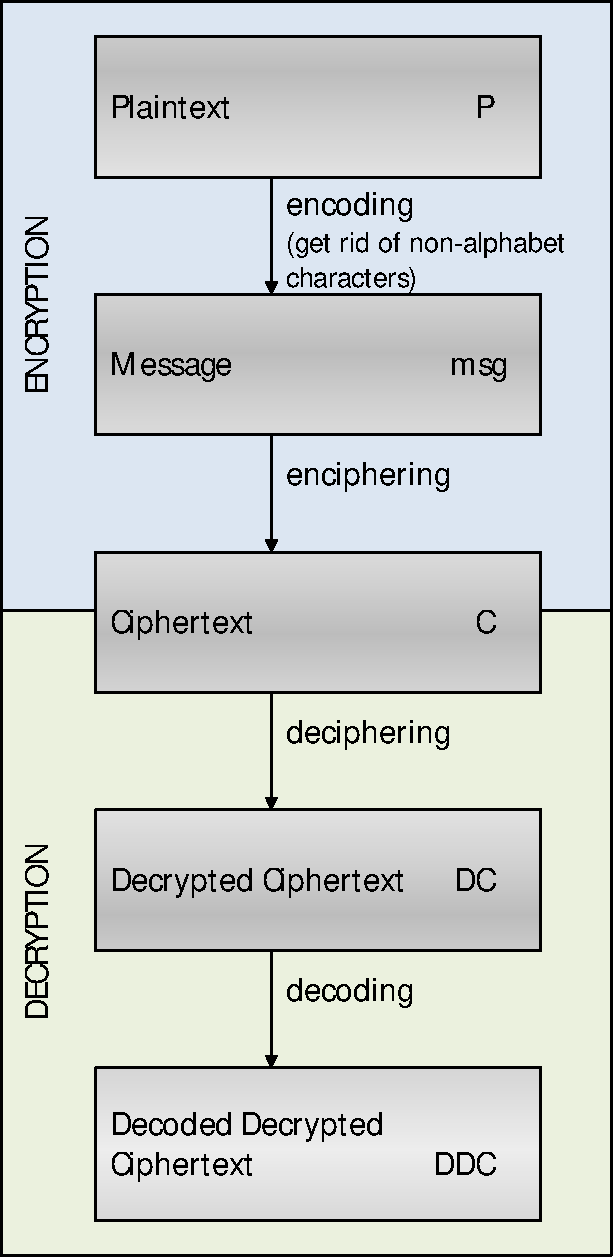
\includegraphics[scale=0.5]{figures/notation-enc-dec_in-sage-scripts_en}
\caption{Structure and naming convention of the SageMath cipher code examples} 
\label{naming-convention-in-Sage-cipher-samples}
\end{center}
\end{figure}



% ---------------------------------------------------------------------------
\newpage
\subsection{Transposition ciphers}
\index{transposition}

Transposition ciphers are implemented in the SageMath class
\begin{center}
\verb!sage.crypto.classical.TranspositionCryptosystem!
\end{center}
To construct and work with a transposition cipher, we first need to
determine the alphabet that contains the symbols used to build the space of our plaintext
and ciphertext. 
Typically, this alphabet will be the upper-case letters of the
English alphabet, which can be accessed via the function
\begin{center}
\verb!sage.monoids.string_monoid.AlphabeticStrings!
\end{center}
We then need to decide on the block length of a block permutation,
which is the length of the row vector to be used in the simple columns
transposition. This row vector is our key, and it specifies a permutation
of a plaintext.

The following first example of transposition ciphers has block length 14,
and the key is build in a way, that every letter
in the plaintext is shifted to the right by two characters, with wrap
around at the end of the block. That is the encryption process. The decryption process is
shifting each letter of the ciphertext to the left by $14 - 2 = 12$.

% Using [fontsize=\footnotesize,fontshape=tt] caused:
%   LaTeX Font Warning: Font shape `T1/cmtt/m/tt' undefined
%   (Font)              using `T1/cmtt/m/n' instead on input line 730.
% so deleted the fontshape parameter.
\begin{sagecode}
\begin{Verbatim}%
[fontsize=\footnotesize]
sage: # transposition cipher using a block length of 14
sage: T = TranspositionCryptosystem(AlphabeticStrings(), 14)
sage: # given plaintext
sage: P   = "a b c d e f g h i j k l m n"
sage: # encryption key
sage: key = [3, 4, 5, 6, 7, 8, 9, 10, 11, 12, 13, 14, 1, 2]
sage:
sage: # encode plaintext (get rid of non-alphabet chars, convert lower-case to upper-case)
sage: msg = T.encoding(P)
sage: # encrypt plaintext by shifting to the left by 2 letters (do it in two steps)
sage: E   = T(key)
sage: C   = E(msg); C
CDEFGHIJKLMNAB
sage:
sage: # decrypt ciphertext by shifting to the left by 12 letters
sage: keyInv = [13, 14, 1, 2, 3, 4, 5, 6, 7, 8, 9, 10, 11, 12]
sage: D   = T(keyInv)
sage: D(C)
ABCDEFGHIJKLMN
sage:
sage: # Representation of key and inverse key as permutations
sage: E
(1,3,5,7,9,11,13)(2,4,6,8,10,12,14)
sage: D
(1,13,11,9,7,5,3)(2,14,12,10,8,6,4)
\end{Verbatim}
\caption{Simple transposition by shifting (key and inverse key explicitly given)}
\end{sagecode}

\newpage
The second example of transposition ciphers is also a simple shifting column transposition.
But now the code is a little bit more automated: The keys are generated from the shift parameter.

\begin{sagecode}
\begin{Verbatim}%
[fontsize=\footnotesize]
sage: # transposition cipher using a block length of 14, code more variable
sage: keylen = 14
sage: shift = 2
sage: A = AlphabeticStrings()
sage: T = TranspositionCryptosystem(A, keylen)
sage:
sage: # construct the plaintext string from the first 14 letters of the alphabet plus blanks
sage: # plaintext   = "A B C D E F G H I J K L M N"
sage: A.gens()
(A, B, C, D, E, F, G, H, I, J, K, L, M, N, O, P, Q, R, S, T, U, V, W, X, Y, Z)
sage: P=''
sage: for i in range(keylen): P=P + " " + str(A.gen(i))
....:
sage: P
' A B C D E F G H I J K L M N'
sage:
sage: # encryption key
sage: # key = [3, 4, 5, 6, 7, 8, 9, 10, 11, 12, 13, 14, 1, 2]
sage: key = [(i+shift).mod(keylen) + 1 for i in range(keylen)]; key
[3, 4, 5, 6, 7, 8, 9, 10, 11, 12, 13, 14, 1, 2]
sage:
sage: # encode plaintext (get rid of non-alphabet chars)
sage: msg = T.encoding(P)
sage: # encrypt plaintext by shifting to the left by 2 letters (do it in one step)
sage: C   = T.enciphering(key, msg); C
CDEFGHIJKLMNAB
sage:
sage: # decrypt ciphertext by shifting to the left by 12 letters
sage: # keyInv = [13, 14, 1, 2, 3, 4, 5, 6, 7, 8, 9, 10, 11, 12]
sage: shiftInv=keylen-shift;
sage: keyInv = [(i+shiftInv).mod(keylen) + 1 for i in range(keylen)]; keyInv
[13, 14, 1, 2, 3, 4, 5, 6, 7, 8, 9, 10, 11, 12]
sage: DC   = T.enciphering(keyInv, C); DC
ABCDEFGHIJKLMN
sage:
sage: # decryption using the "deciphering method with key" instead of "enciphering with keyInv" 
sage: # using the deciphering method requires to change the type of the variable key
sage: DC  = T.deciphering(T(key).key(), C); DC
ABCDEFGHIJKLMN
sage:
sage: # representation of key and inverse key as permutations
sage: T(key)
(1,3,5,7,9,11,13)(2,4,6,8,10,12,14)
sage: T(key).key()
(1,3,5,7,9,11,13)(2,4,6,8,10,12,14)
sage: T(keyInv)
(1,13,11,9,7,5,3)(2,14,12,10,8,6,4)
\end{Verbatim}
\caption{Simple transposition by shifting (key and inverse key constructed with ``range'')}
\end{sagecode}

\newpage
In the third example of transposition ciphers we use an arbitrary permutation as key in the
encryption and decryption processes in order to scramble the characters within each
block (block length = number of columns in a simple column transposition).
If the block length is $n$, then the key must be a permutation on $n$ symbols.
The following example uses the method \verb!random_key()! of the class
\verb!TranspositionCryptosystem!. Each call to \verb!random_key()! produces a
different key. Note that therefore your results (key and ciphertext) may be different
from the following example.

\begin{sagecode}
\begin{Verbatim}%
[fontsize=\footnotesize]
sage: # Remark: Enciphering here requires, that the length of msg is a multiple of keylen
sage: keylen = 14   # length of key
sage: A = AlphabeticStrings()
sage: T = TranspositionCryptosystem(A, keylen); T
Transposition cryptosystem on Free alphabetic string monoid on A-Z of block length 14
sage:
sage: P = "a b c d e f g h i j k l m n o p q r s t u v w x y z a b"
sage: key = T.random_key(); key
(1,2,3,13,6,5,4,12,7)(11,14)
sage: msg = T.encoding(P); msg
ABCDEFGHIJKLMNOPQRSTUVWXYZAB
sage: C   = T.enciphering(key, msg); C
BCMLDEAHIJNGFKPQAZRSOVWXBUTY
sage: # decryption using the "deciphering method with key" instead of "enciphering with keyInv" 
ssage: DC  = T.deciphering(key, C); DC
ABCDEFGHIJKLMNOPQRSTUVWXYZAB
sage:
sage: # Just another way of decryption: Using "enciphering" with the inverse key
sage: keyInv = T.inverse_key(key); keyInv
(1,7,12,4,5,6,13,3,2)(11,14)
sage: DC     = T.enciphering(keyInv, C); DC
ABCDEFGHIJKLMNOPQRSTUVWXYZAB
sage:
sage: # Test correctness of decryption
sage: msg == DC
True
\end{Verbatim}
\caption{Simple column transposition with randomly generated (permutation) key}
\end{sagecode}


\newpage
The fourth example of transposition ciphers additionally shows the key space of a simple
column transposition.

\begin{sagecode}
\begin{Verbatim}%
[fontsize=\footnotesize]
sage: keylen = 14   # length of key
sage: A = AlphabeticStrings()
sage: T = TranspositionCryptosystem(A, keylen); T
Transposition cryptosystem on Free alphabetic string monoid on A-Z of block length 14
sage: T.key_space()
Symmetric group of order 14! as a permutation group
sage: # Remark: The key space is not quite correct as also permutations shorter than keylen are counted.
sage:
sage: P = "a b c d e f g h i j k l m n o p q r s t u v w x y z a b"
sage: key = T.random_key(); key
(1,2,7)(3,9)(4,5,10,12,8,13,11)(6,14)
sage: msg = T.encoding(P); msg
ABCDEFGHIJKLMNOPQRSTUVWXYZAB
sage:
sage: # enciphering in one and in two steps
sage: C   = T.enciphering(key, msg); C
BGIEJNAMCLDHKFPUWSXBOAQZRVYT
sage:
sage: enc = T(key); enc.key()
(1,2,7)(3,9)(4,5,10,12,8,13,11)(6,14)
sage: C = enc(msg); C
BGIEJNAMCLDHKFPUWSXBOAQZRVYT
sage:
sage: # deciphering
sage: DC  = T.deciphering(key, C); DC
ABCDEFGHIJKLMNOPQRSTUVWXYZAB
\end{Verbatim}
\caption{Simple column transposition (showing the size of the key space)}% the key\_space
\end{sagecode}



% ---------------------------------------------------------------------------
\newpage
\subsection{Substitution ciphers}
\index{substitution}

Substitution cryptosystems are implemented in SageMath in the class
\begin{center}
\verb!sage.crypto.classical.SubstitutionCryptosystem!
\end{center}

\noindent The following code sample uses SageMath to construct a substitution
cipher with a random key. A random key can be generated using the
method \verb!random_key()! of the class
\texttt{SubstitutionCryp\-to\-system}. Different keys determine different
substitution ciphers. So each call to \verb!random_key()! returns
different results.

\begin{sagecode}
\begin{Verbatim}%
[fontsize=\footnotesize]
sage: # plaintext/ciphertext alphabet
sage: A   = AlphabeticStrings()
sage: S   = SubstitutionCryptosystem(A)
sage:
sage: P   = "Substitute this with something else better."
sage: key = S.random_key(); key
INZDHFUXJPATQOYLKSWGVECMRB
sage:
sage: # method encoding can be called from A or from T
sage: msg = A.encoding(P); msg
SUBSTITUTETHISWITHSOMETHINGELSEBETTER
sage: C   = S.enciphering(key, msg); C
WVNWGJGVGHGXJWCJGXWYQHGXJOUHTWHNHGGHS
sage:
sage: # We now decrypt the ciphertext to recover our plaintext.
sage:
sage: DC  = S.deciphering(key, C); DC
SUBSTITUTETHISWITHSOMETHINGELSEBETTER
sage: msg == DC
True
\end{Verbatim}
\caption{Monoalphabetic substitution with randomly generated key}
\end{sagecode}



% ---------------------------------------------------------------------------
\newpage
\subsubsection{Caesar cipher}
\index{Caesar cipher}

The following example uses SageMath to construct a Caesar cipher.

\begin{sagecode}
\begin{Verbatim}%
[fontsize=\footnotesize]
sage: # plaintext/ciphertext alphabet
sage: A = AlphabeticStrings()
sage: P = "Shift the alphabet three positions to the right."
sage:
sage: # construct Caesar cipher
sage: S = SubstitutionCryptosystem(A)
sage: key = A([3, 4, 5, 6, 7, 8, 9, 10, 11, 12, 13, 14, 15, 16, 17, 18, 19, \
....:          20, 21, 22, 23, 24, 25, 0, 1, 2])
sage:
sage: # encrypt message
sage: msg     = A.encoding(P); msg
SHIFTTHEALPHABETTHREEPOSITIONSTOTHERIGHT
sage: encrypt = S(key); encrypt
DEFGHIJKLMNOPQRSTUVWXYZABC
sage: C       = encrypt(msg); C
VKLIWWKHDOSKDEHWWKUHHSRVLWLRQVWRWKHULJKW
sage:
sage: # Next, we recover the plaintext.
sage: # decrypt message
sage: keyInv = A([23, 24, 25, 0, 1, 2, 3, 4, 5, 6, 7, 8, 9, 10, 11, 12, 13, \
....:             14, 15, 16, 17, 18, 19, 20, 21, 22])
sage: decrypt = S(keyInv); decrypt
XYZABCDEFGHIJKLMNOPQRSTUVW
sage: DC      = decrypt(C); DC
SHIFTTHEALPHABETTHREEPOSITIONSTOTHERIGHT
sage: msg == DC
True
\end{Verbatim}
\caption{Caesar (substitution by shifting the alphabet; key explicitly given, step-by-step approach)}
\end{sagecode}


\newpage
\noindent The second Caesar sample does the same, but the code is more
sophisticated/automated/fle\-xi\-ble.

\begin{sagecode}
\begin{Verbatim}%
[fontsize=\footnotesize]
sage: # plaintext/ciphertext alphabet
sage: A = AlphabeticStrings()
sage: keylen = len(A.gens()); keylen
26
sage: shift  = 3
sage: P = "Shift the alphabet three positions to the right."
sage:
sage: # construct Caesar cipher
sage: S = SubstitutionCryptosystem(A)
sage: S
Substitution cryptosystem on Free alphabetic string monoid on A-Z
sage: # key = A([3, 4, 5, 6, 7, 8, 9, 10, 11, 12, 13, 14, 15, 16, 17, 18, 19, \
sage: #          20, 21, 22, 23, 24, 25, 0, 1, 2])
sage: key = [(i+shift).mod(keylen) for i in range(keylen)];
sage: key = A(key); key
DEFGHIJKLMNOPQRSTUVWXYZABC
sage: len(key)
26
sage:
sage: # encrypt message
sage: msg     = A.encoding(P); msg
SHIFTTHEALPHABETTHREEPOSITIONSTOTHERIGHT
sage: C       = S.enciphering(key, msg); C
VKLIWWKHDOSKDEHWWKUHHSRVLWLRQVWRWKHULJKW
sage:
sage: # Next, we recover the plaintext.
sage: # decrypt message
sage: # keyInv = A([23, 24, 25, 0, 1, 2, 3, 4, 5, 6, 7, 8, 9, 10, 11, 12, 13, \
sage: #             14, 15, 16, 17, 18, 19, 20, 21, 22])
sage: shiftInv=keylen-shift;
sage: keyInv = [(i+shiftInv).mod(keylen) for i in range(keylen)];
sage: keyInv = A(keyInv); keyInv
XYZABCDEFGHIJKLMNOPQRSTUVW
sage: DC     = S.enciphering(keyInv, C); DC
SHIFTTHEALPHABETTHREEPOSITIONSTOTHERIGHT
sage:
sage: # Just another way of decryption: Using "deciphering" with the key
sage: DC     = S.deciphering(key, C); DC
SHIFTTHEALPHABETTHREEPOSITIONSTOTHERIGHT
sage:
sage: msg == DC
True
\end{Verbatim}
\caption{Caesar (substitution by shifting the alphabet; substitution key generated)}
\end{sagecode}


% ---------------------------------------------------------------------------
\newpage
\subsubsection{Shift cipher}
\index{shift cipher}

The shift cipher can also be thought of as a generalization of the Caesar
cipher. While the Caesar cipher restricts us to shift exactly three
positions along an alphabet, the shift cipher allows us to shift any
number of positions along the alphabet.

In the above samples we applied the \verb!SubstitutionCryptosystem!
and build Caesar as a special kind of substitution. In contrast here
Caesar can be build as a special kind of the shift cipher.

The shift cipher is implemented directly in the SageMath class
\begin{center}
\verb!sage.crypto.classical.ShiftCryptosystem!
\end{center}

In the following example, we construct a shift cipher over the capital
letters of the English alphabet. We then encrypt a plaintext P by
shifting it 12 positions along the alphabet. Finally, we decrypt the
ciphertext C and make sure that the result (DC) is indeed the original
plaintext. Shifting is a special way of substitution.

\begin{sagecode}
\begin{Verbatim}%
[fontsize=\footnotesize]
sage: # construct Shift cipher directly
sage: shiftcipher = ShiftCryptosystem(AlphabeticStrings()); shiftcipher
Shift cryptosystem on Free alphabetic string monoid on A-Z
sage: P = shiftcipher.encoding("Shift me any number of positions."); P
SHIFTMEANYNUMBEROFPOSITIONS
sage: key = 12  # shift can be any integer number
sage: 
sage: # shift the plaintext by 12 positions to get the ciphertext
sage: C = shiftcipher.enciphering(key, P); C
ETURFYQMZKZGYNQDARBAEUFUAZE
sage: 
sage: # decrypt the ciphertext and ensure that it is the original plaintext
sage: DC = shiftcipher.deciphering(key, C); DC
SHIFTMEANYNUMBEROFPOSITIONS
sage: DC == P
True
\end{Verbatim}
\caption{A shift cipher over the upper-case letters of the English alphabet}
\label{paper_pencil:shift_cipher:Sage_example}
\end{sagecode}

The Caesar cipher is simply a shift cipher whose shifting key is 3. In
the next example, we use the shift cipher to create a Caesar cipher
over the capital letters of the English alphabet. % We then encrypt a
% plaintext P using the Caesar cipher, and then proceed to decrypt the
% resulting ciphertext C. Finally, we ensure that the decrypted result is
% the same as our original plaintext.

\begin{sagecode}
\begin{Verbatim}%
[fontsize=\footnotesize]
sage: # create a Caesar cipher
sage: caesarcipher = ShiftCryptosystem(AlphabeticStrings())
sage: P = caesarcipher.encoding("Shift the alphabet by three positions to the right."); P
SHIFTTHEALPHABETBYTHREEPOSITIONSTOTHERIGHT
sage: 
sage: key = 3  # shift the plaintext by exactly 3 positions
sage: C = caesarcipher.enciphering(key, P); C
VKLIWWKHDOSKDEHWEBWKUHHSRVLWLRQVWRWKHULJKW
sage: 
sage: # decrypt the ciphertext and ensure that it is the original plaintext
sage: DC = caesarcipher.deciphering(key, C); DC
SHIFTTHEALPHABETBYTHREEPOSITIONSTOTHERIGHT
sage: DC == P
True
\end{Verbatim}
\caption{Constructing the Caesar cipher using the shift cipher}
\label{paper_pencil:shift_cipher:Sage_example_Caesar_cipher}
\end{sagecode}


% ---------------------------------------------------------------------------
\newpage
\subsubsection{Affine cipher}
\label{PaP_affine_cipher_sage-sample}
\index{affine cipher}

The affine cipher is implemented in the SageMath class
\begin{center}
\verb!sage.crypto.classical.AffineCryptosystem!
\end{center}

In the following example, we construct an affine cipher $ c_i = b*p_i + a $
with key $(3, 13)$ and use this key to encrypt a given plaintext
$P = (p_1,p_2, ...,p_n)$. The plaintext is then decrypted and the result
DC is compared to the original plaintext.

\begin{sagecode}
\begin{Verbatim}%
[fontsize=\footnotesize]
sage: # create an affine cipher
sage: affineCipher = AffineCryptosystem(AlphabeticStrings()); affineCipher
Affine cryptosystem on Free alphabetic string monoid on A-Z
sage: P = affineCipher.encoding("The affine cryptosystem.")
sage: P
THEAFFINECRYPTOSYSTEM
sage: 
sage: # encrypt the plaintext using the key (3, 13)
sage: a, b = (3, 13)
sage: C = affineCipher.enciphering(a, b, P)
sage: C
SIZNCCLAZTMHGSDPHPSZX
sage: 
sage: # decrypt the ciphertext and make sure that it is equivalent to the original plaintext
sage: DC = affineCipher.deciphering(a, b, C)
sage: DC
THEAFFINECRYPTOSYSTEM
sage: DC == P
True
\end{Verbatim}
\caption{An affine cipher with key $(3, 13)$}
\end{sagecode}


We can also construct a shift cipher using the affine cipher. To do
so, we need to restrict keys of the affine cipher be of the form 
$(1, b)$ where $b$ is any non-negative integer. For instance, we can
work through SageMath example~\ref{paper_pencil:shift_cipher:Sage_example} on
page~\pageref{paper_pencil:shift_cipher:Sage_example} as follows:

\begin{sagecode}
\begin{Verbatim}%
[fontsize=\footnotesize]
sage: # construct a shift cipher
sage: shiftcipher = AffineCryptosystem(AlphabeticStrings()); shiftcipher
Affine cryptosystem on Free alphabetic string monoid on A-Z
sage: P = shiftcipher.encoding("Shift me any number of positions.")
sage: P
SHIFTMEANYNUMBEROFPOSITIONS
sage: 
sage: # shift the plaintext by 12 positions to get the ciphertext
sage: a, b = (1, 12)
sage: C = shiftcipher.enciphering(a, b, P)
sage: C
ETURFYQMZKZGYNQDARBAEUFUAZE
sage: 
sage: # decrypt the ciphertext and ensure that it is the original plaintext
sage: DC = shiftcipher.deciphering(a, b, C); P
SHIFTMEANYNUMBEROFPOSITIONS
sage: DC == P
True
\end{Verbatim}
\caption{Constructing a shift cipher using the affine cipher}
\end{sagecode}


We can also use the affine cipher to create the Caesar cipher. To do
so, the encryption/decryption key must be $(1, 3)$. In the next
example, we work through SageMath
example~\ref{paper_pencil:shift_cipher:Sage_example_Caesar_cipher} on
page~\pageref{paper_pencil:shift_cipher:Sage_example_Caesar_cipher}
using the affine cipher.

\begin{sagecode}
\begin{Verbatim}%
[fontsize=\footnotesize]
sage: # create a Caesar cipher
sage: caesarcipher = AffineCryptosystem(AlphabeticStrings())
sage: P = caesarcipher.encoding("Shift the alphabet by three positions to the right.")
sage: P
SHIFTTHEALPHABETBYTHREEPOSITIONSTOTHERIGHT
sage: 
sage: # shift the plaintext by 3 positions
sage: a, b = (1, 3)
sage: C = caesarcipher.enciphering(a, b, P)
sage: C
VKLIWWKHDOSKDEHWEBWKUHHSRVLWLRQVWRWKHULJKW
sage: 
sage: # decrypt the ciphertext and ensure that it is the original plaintext
sage: DC = caesarcipher.deciphering(a, b, C)
sage: DC
SHIFTTHEALPHABETBYTHREEPOSITIONSTOTHERIGHT
sage: DC == P
True
\end{Verbatim}
\caption{Constructing the Caesar cipher using the affine cipher}
\end{sagecode}



% ---------------------------------------------------------------------------
\newpage
\subsubsection{Substitution with symbols}
\index{substitution}

In the following SageMath example the symbols are from the binary number
system. A monoalphabetic substitution cipher with a binary alphabet has very little
security: Because the plaintext/ciphertext alphabet has only the two elements
0 and 1, there are only two keys possible: (0 1) and (1 0). \\
Remark: The key of a general substitution cipher contains all symbols
of the alphabet exactly once.

\begin{sagecode}
\begin{Verbatim}%
[fontsize=\footnotesize]
sage: # the plaintext/ciphertext alphabet
sage: B = BinaryStrings()
sage: # substitution cipher over the alphabet B; no keylen argument possible
sage: S = SubstitutionCryptosystem(B); S
Substitution cryptosystem on Free binary string monoid
sage: # To get a substitute for each symbol, key has always the length of the alphabet
sage: key = S.random_key(); key
10
sage: len(key)
2
sage: P = "Working with binary numbers."
sage: # encryption
sage: msg = B.encoding(P); msg
01010111011011110111001001101011011010010110111001100111001000000111011101101\
00101110100011010000010000001100010011010010110111001100001011100100111100100\
1000000110111001110101011011010110001001100101011100100111001100101110
sage: C   = S.enciphering(key, msg); C
10101000100100001000110110010100100101101001000110011000110111111000100010010\
11010001011100101111101111110011101100101101001000110011110100011011000011011\
0111111001000110001010100100101001110110011010100011011000110011010001
sage: # decryption
sage: DC  = S.deciphering(key, C); DC
01010111011011110111001001101011011010010110111001100111001000000111011101101\
00101110100011010000010000001100010011010010110111001100001011100100111100100\
1000000110111001110101011011010110001001100101011100100111001100101110
sage: msg == DC
True
\end{Verbatim}
\caption{Monoalphabetic substitution with a binary alphabet}
\end{sagecode}

Remark: Currently \verb!S! has no attribute \verb!key!, and I found no way
to transform the binary sequence \verb!DC! back to ASCII.



\newpage
The second sample of a monoalphabetic substitution with symbols uses  a larger alphabet
as plaintext/ciphertext space as the first sample. Here the hexadecimal number system
is used as substitution alphabet.

\begin{sagecode}
\begin{Verbatim}%
[fontsize=\footnotesize]
sage: A = HexadecimalStrings()
sage: S = SubstitutionCryptosystem(A)
sage: key = S.random_key(); key
2b56a4e701c98df3
sage: len(key)
16
sage: # Number of possible keys
sage: factorial(len(key))
20922789888000
sage: P   = "Working with a larger alphabet."
sage:
sage: msg = A.encoding(P); msg
576f726b696e6720776974682061206c617267657220616c7068616265742e
sage: C   = S.enciphering(key, msg); C
47e375e9e1efe75277e17ae052eb52e8eb75e7e47552ebe872e0ebe5e47a5f
sage: DC  = S.deciphering(key, C); DC
576f726b696e6720776974682061206c617267657220616c7068616265742e
sage: msg == DC
True
sage:
sage: # Conversion hex back to ASCII:
sage: # - AlphabeticStrings() and HexadecimalStrings() don't have according methods.
sage: # - So we used Python directly.
sage: import binascii
sage: DDC = binascii.a2b_hex(repr(DC)); DDC
'Working with a larger alphabet.'
sage:
sage: P == DDC
True
\end{Verbatim}
\caption{Monoalphabetic substitution with a hexadecimal alphabet (and decoding in Py\-thon)}
\end{sagecode}



% ---------------------------------------------------------------------------
\newpage
\subsubsection{Vigen{\`e}re cipher}
\index{Vigen\`ere}

The Vigen{\`e}re cipher is implemented in the SageMath class
\begin{center}
\verb!sage.crypto.classical.VigenereCryptosystem!
\end{center}

\noindent For our ciphertext/plaintext space, we can work with the upper-case
letters of the English alphabet, the binary number system, the
octal number system, or the hexadecimal number system. Here is an
example using the class \verb!AlphabeticStrings!, which implements
the English capital letters.

\begin{sagecode}
\begin{Verbatim}%
[fontsize=\footnotesize]
sage: # construct Vigenere cipher
sage: keylen = 14
sage: A = AlphabeticStrings()
sage: V = VigenereCryptosystem(A, keylen); V
Vigenere cryptosystem on Free alphabetic string monoid on A-Z of period 14
sage:
sage: # alternative could be a given key: key = A('ABCDEFGHIJKLMN'); key
sage: key = V.random_key(); key
WSSSEEGVVAARUD
sage: len(key)
14
sage:
sage: # encoding
sage: P = "The Vigenere cipher is polyalphabetic."
sage: len(P)
38
sage: msg = V.encoding(P); msg     # alternative: msg = A.encoding(P); msg
THEVIGENERECIPHERISPOLYALPHABETIC
sage:
sage: # encryption [2 alternative ways (in two steps or in one): both work]
sage: # encrypt = V(key); encrypt
sage: # C = encrypt(msg); C
sage: C   = V.enciphering(key, msg); C
PZWNMKKIZRETCSDWJAWTUGTALGBDXWLAG
sage:
sage: # decryption
sage: DC  = V.deciphering(key, C); DC
THEVIGENERECIPHERISPOLYALPHABETIC
sage: msg == DC
True
\end{Verbatim}
\caption{Vigen{\`e}re cipher}
\end{sagecode}




% ---------------------------------------------------------------------------
\newpage
\subsection{Hill cipher}
\index{Hill}

The Hill~\cite{pp:Hill1929,pp:Hill1931} or matrix cipher is
mathematically more sophisticated than the other ciphers mentioned in this
chapter. The encryption/decryption key of this cipher is an invertible
square matrix (here called $key$).
Plaintext and ciphertext are vectors ($P$ and $C$).
The encryption and decryption processes use matrix operations modulo 26,
here it is $C = P * key$ $(mod$ $26)$. %Zweimal $$-Klammer, damit Blank vor "(".

\noindent The Hill cipher is implemented in the SageMath class
\begin{center}
\verb!sage.crypto.classical.HillCryptosystem!
\end{center}

\noindent In the following example our plaintext/ciphertext space is the
capital letters of the English alphabet. In the Hill cipher, each
letter of this alphabet is assigned a unique integer modulo 26.
The size of the key matrix (also called its dimension) is not restricted by the
cipher.\\

\noindent {\bf Remark:} Comparing the Hill implementation in CrypTool v1.4.31
and in SageMath version 5.3:
\begin{itemize}
  \item SageMath offers fast command-line operations; CT1 offers
        its functionality within a GUI.
  \item SageMath offers for the key matrix any dimension; CT1 is restricted
        to a matrix size between 1 and 10.
  \item SageMath allows negative numbers in the key matrix, and converts them
        automatically into appropriate non-negative numbers;
        CT1 doesn't allow negative numbers in the key matrix.
  \item SageMath always sets the first alphabet character to 0;\\
        SageMath only allows the 26 capital letters as alphabet;\\
        and it uses only the multiplication variant
        plaintext row vector * key matrix:\\
        $C = P * key$.
  \item CT1 offers to choose also 1 as value for the first alphabet
        character; you can combine your alphabet within the text options dialog;
        and it also offers to use a reverse multiplication variant:
        $C = key * P$.
\end{itemize}

\begin{figure}[ht]
\begin{center}
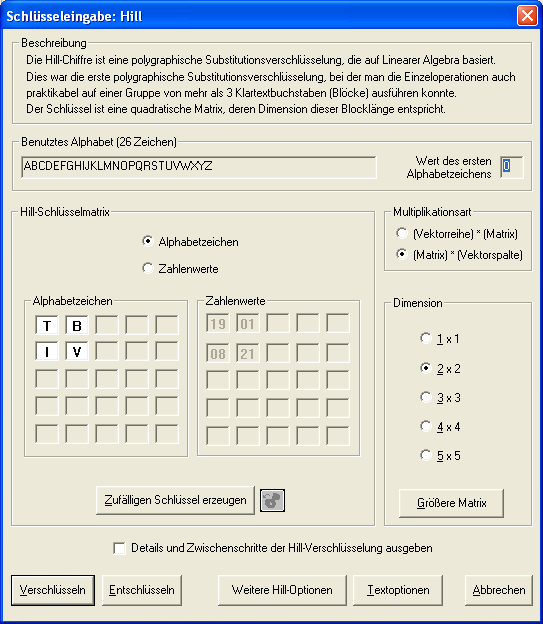
\includegraphics[scale=0.7]{figures/PaP_Fig_Hill-Cipher-CT-Dialog.png}
\caption{Hill dialog in CT1 with the operations and options available\vspace{1ex}} 
\label{PaP_Fig_Hill-Cipher-CT-Dialog}
\end{center}
\end{figure}


\begin{sagecode}
\begin{Verbatim}%
[fontsize=\footnotesize]
sage: # construct a Hill cipher
sage: keylen = 19    # An Alternative could be: Use a non-random small key (e.g. keylen = 3)
sage: A = AlphabeticStrings(); H = HillCryptosystem(A, keylen); H
Hill cryptosystem on Free alphabetic string monoid on A-Z of block length 19
sage:
sage: # Alternative: Here, HKS is necessary in addition [H.key_space() isn't enough].
sage: # HKS = H.key_space(); key = HKS([[1,0,1],[0,1,1],[2,2,3]]); key
sage:
sage: # Random key creation
sage: key = H.random_key(); key
[10  7  5  2  0  6 10 23 15  7 17 19 18  2  9 12  0 10 11]
[23  1  1 10  4  9 21  1 25 22 19  8 17 22 15  8 12 25 22]
[ 4 12 16 15  1 12 24  5  9 13  5 15  8 21 23 24 22 20  6]
[ 5 11  6  7  3 12  8  9 21 20  9  4 16 18 10  3  2 23 18]
[ 8 22 14 14 20 13 21 19  3 13  2 11 13 23  9 25 25  6  8]
[24 25  8 24  7 18  3 20  6 11 25  5  6 19  7 24  2  4 10]
[15 25 11  1  4  7 11 24 20  2 18  4  9  8 12 19 24  0 12]
[14  6  2  9 11 20 13  4 10 11  4 23 14 22 14 16  9 12 18]
[12 10 21  5 21 15 16 17 19 20  1  1 15  5  0  2 23  4 14]
[21 15 15 16 15 20  4 10 25  7 15  4  7 12 24  9 19 10  6]
[25 15  2  3 17 23 21 16  8 18 23  4 22 11 15 19  6  0 15]
[14 23  9  3 18 15 10 18  7  5 12 23 11  9 22 21 20  4 14]
[ 3  6  8 13 20 16 11  1 13 10  4 21 25 15 12  3  0 11 18]
[21 25 14  6 11  3 21  0 19 17  5  8  5  4  9  2 23 19 15]
[ 8 11  9 11 20 15  6  1  3 18 18 22 16 17  6  3 15 11  2]
[21 15  5 22  2  9  0  4 22 10  2 10 19 19 17 19  1 21  4]
[ 7 17  9  2 15  5 14  3  6  9 12 12 22 15  8  4 21 14 19]
[19 14 24 19  7  5 22 22 13 14  7 18 17 19 25  2  1 23  6]
[ 2  6 14 22 17  7 23  6 22  7 13 20  0 14 23 17  6  1 12]
sage:
sage: # encoding and encryption
sage: P = "Hill or matrix cipher uses matrix operations."; len(P)
45
sage: # implementation requires: Length of msg is a multiple of matrix dimension (block_length)
sage: msg = H.encoding(P); msg; len(msg)
HILLORMATRIXCIPHERUSESMATRIXOPERATIONS
38
sage:
sage: # encryption (the length of msg must be a multiple of keylen).
sage: C  = H.enciphering(key, msg); C
CRWCKPRVYXNBRZTNZCTQWFWSDWBCHABGMNEHVP
sage:
sage: # decryption
sage: DC  = H.deciphering(key, C); DC; msg == DC
HILLORMATRIXCIPHERUSESMATRIXOPERATIONS
True
sage:
sage: # alternative decryption using inverse matrix
sage: keyInv = H.inverse_key(key); keyInv
[ 6 23  1 23  3 12 17 22  6 16 22 14 18  3  1 10 21 16 20]
[18 23 15 25 24 23  7  4 10  7 21  7  9  0 13 22  5  5 23]
...
[10 11 12  6 11 17 13  9 19 16 14 24  4  8  5 16 18 20  1]
[19 16 16 21  1 19  7 12  3 18  1 17  7 10 24 21  7 16 11]
sage: DC     = H.enciphering(keyInv, C); DC
HILLORMATRIXCIPHERUSESMATRIXOPERATIONS
\end{Verbatim}
\caption{Hill cipher with randomly generated key matrix}
\end{sagecode}







% --------------------------------------------------------------------------
\newpage
\begin{thebibliography}{99999}
\addcontentsline{toc}{section}{Bibliography}

\bibitem[ACA2002]{pp:ACA2002} \index{ACA 2002}
   American Cryptogram Association, \\
   {\em Length and Standards for all ACA Ciphers}, 2002.\\
   \url{http://www.cryptogram.org/cdb/aca.info/aca.and.you/chap08.html#},\\
   \url{http://www.und.edu/org/crypto/crypto/.chap08.html}

\bibitem[Bauer1995]{pp:Bauer1995} \index{Bauer 1995}
    Friedrich L. Bauer, \\
    {\em Entzifferte Geheimnisse},\\
    Springer, 1995.

\bibitem[Bauer2000]{pp:Bauer2000} \index{Bauer 2000}
    Friedrich L. Bauer, \\
    {\em Decrypted Secrets}, Springer 1997,\\
    2nd edition 2000.
	
\bibitem[Crowley2000]{pp:Crowley2000} \index{Crowley 2000}
   Paul Crowley, \\
   {\em Mirdek: A card cipher inspired by ``Solitaire''}, 2000.\\
   \url{http://www.ciphergoth.org/crypto/mirdek/}

\bibitem[DA1999]{pp:DA1999} \index{DA 1999}
   Data encryption page of the ThinkQuest Team 27158 for ThinkQuest 1999 \\
   (no update since 1999, no search possibility), 1999.\\
   \url{http://library.thinkquest.org/27158/}

\bibitem[Goebel2003]{pp:Goebel2003} \index{Goebel 2003}
   Greg Goebel, \\
   {\em Codes, Ciphers and Codebreaking}, 2003.\\
   \url{http://www.vectorsite.net/ttcode.htm}

\bibitem[Hill1929]{pp:Hill1929} \index{Hill 1929}
   Lester S. Hill,\\
   \emph{Cryptography in an Algebraic Alphabet},\\
   The American Mathematical Monthly, 36(6): 306--312, 1929.

\bibitem[Hill1931]{pp:Hill1931} \index{Hill 1931}
   Lester S. Hill,\\
   \emph{Concerning Certain Linear Transformation Apparatus of Cryptography},\\
   The American Mathematical Monthly, 38(3): 135--154, 1931.

\bibitem[Nichols1996]{pp:Nichols1996} \index{Nichols 1996} 
    Randall K. Nichols, \\
    {\em Classical Cryptography Course, Volume 1 and 2}, \\
    Aegean Park Press 1996;\\
    or in 12 lessons online at \\
    \url{http://www.fortunecity.com/skyscraper/coding/379/lesson1.htm}

\bibitem[Nguyen2009]{pp:Nguyen2009} \index{Nguyen 2009} 
       Minh Van Nguyen, \\
       {\em Exploring Cryptography Using the SageMath Computer Algebra System}, \\
       Victoria University, 2009, \\
       See SageMath publications\\
       \url{http://www.sagemath.org/library-publications.html},\\
       \url{http://www.sagemath.org/files/thesis/nguyen-thesis-2009.pdf},\\
       \url{http://sites.google.com/site/nguyenminh2/honours-thesis-2009.pdf}

\bibitem[Savard1999]{pp:Savard1999} \index{Savard 1999}
	John J. G. Savard, \\
	{\em A Cryptographic Compendium}, 1999.\\
	\url{http://www.quadibloc.com/crypto/jscrypt.htm}

\bibitem[Schmeh2004]{pp:Schmeh2004}  \index{Schmeh 2004}
        Klaus Schmeh, \\
        {\em Die Welt der geheimen Zeichen. Die faszinierende Geschichte
        der Verschl\"usselung},\\ 
        W3L Verlag Bochum, 1st edition 2004.

\bibitem[Schmeh2007]{pp:Schmeh2007}  \index{Schmeh 2007}
        Klaus Schmeh, \\
        {\em Codeknacker gegen Codemacher. Die faszinierende Geschichte der Verschl\"usselung},\\ 
        W3L Verlag Bochum, 2nd edition 2007.\\
	This is most current among the books dealing in a comprehensive manner
	with the history of cryptology. It also contains a small collection of
        solved and unsolved crypto riddles. One of the challenges deals with
        a double column transposition using two long keys, which are
        differently in addition.\\
	\url{http://www.mysterytwisterc3.org/en/challenges/level-x/double-column-transposition}

\bibitem[Schneier1999]{pp:Schneier1999}
	Bruce Schneier, \\
	{\em The Solitaire Encryption Algorithm}, \\
	version 1.2, 1999.\\
	\url{http://www.schneier.com/solitaire.html}

\bibitem[Singh1999]{pp:Singh1999} \index{Singh 1999}
	Simon Singh, \\
	{\em The Code Book: The Science of Secrecy from Ancient Egypt to Quantum Cryptography}, \\
	Anchor, 1999.

\bibitem[ThinkQuest1999]{pp:ThinkQuest1999} \index{ThinkQuest 1999}
	ThinkQuest Team 27158, \\
	{\em Data Encryption}, 1999.\\
	\url{http://library.thinkquest.org/27158/}

\end{thebibliography}  % English









% Local Variables:
% TeX-master: "../script-en.tex"
% End:


% $Id: primes.tex 3715 2016-04-10 18:18:55Z esslinger $
% ...........................................................................
%       K A P I T E L  3 :     P R I M Z A H L E N
%
% - Todo for new version: always check "Eyecatcher_neue-Mersenne" in primes.text and numbertheory.tex!
% ~~~~~~~~~~~~~~~~~~~~~~~~~~~~~~~~~~~~~~~~~~~~~~~~~~~~~~~~~~~~~~~~~~~~~~~~~~~

\newpage
% \hypertarget{Kapitel_2}{}
\chapter{Primzahlen}
\label{Label_Kapitel_Primes}  %Die Kapitelnr. von \label wird per per \ref geholt.
(Bernhard Esslinger, Mai 1999; Updates: Nov. 2000, Dez. 2001, Juni 2003, Mai 2005, M�rz 2006, Juni 2007, Jan. 2010, Aug. 2013, M�rz 2016)

\begin{ctsquote}
    Der Fortschritt lebt vom Austausch des Wissens.
\caption[Albert Einstein]{Albert Einstein\footnotemark}
\end{ctsquote}
\addtocounter{footnote}{0}\footnotetext{%
  Albert Einstein, deutscher Physiker und Nobelpreistr�ger, 
  14.03.1879$-$14.04.1955.
}

% --------------------------------------------------------------------------
\section{Was sind Primzahlen?}
\index{Primzahl} \index{Zahlen!Primzahl} Primzahlen sind ganze,
positive Zahlen gr��er gleich $2$, die man nur durch 1 und durch
sich selbst teilen kann. Alle anderen nat�rlichen Zahlen gr��er gleich $4$
sind zusammengesetzte Zahlen und lassen sich durch Multiplikation von
Primzahlen bilden.

\noindent Somit bestehen die {\em nat�rlichen} \index{Zahlen} Zahlen
$ \mathbb{N} = \{1, 2, 3, 4,\cdots \} $ aus
\begin{itemize}
   \item der Zahl $1$ (dem Einheitswert)
   \item den Primzahlen (primes) und
   \item den zusammengesetzten Zahlen (composite numbers).
\end{itemize}

\noindent Primzahlen haben aus drei Gr�nden besondere Bedeutung erlangt:
\begin{itemize}
  \item Sie werden in der Zahlentheorie als die Grundbausteine der
        nat�rlichen Zahlen betrachtet, anhand derer eine Menge genialer
        mathematischer �berlegungen gef�hrt wurden.
  \item Sie haben in der modernen \index{Kryptographie!moderne} Kryptographie
        (Public-Key-Kryptographie\index{Kryptographie!Public-Key}) gro�e
        praktische Bedeutung erlangt. Das verbreiteteste Public-Key-Verfahren
        ist die Ende der siebziger Jahre erfundene \index{RSA} 
        RSA-Verschl�sselung. Nur die Verwendung (gro�er) Primzahlen f�r
        bestimmte Parameter garantiert die Sicherheit des Algorithmus sowohl
        beim RSA-Verfahren als auch bei noch moderneren Verfahren
        (z.B. Elliptische Kurven).
  \item Die Suche nach den gr��ten bekannten Primzahlen hat wohl bisher
        keine praktische Verwendung, erfordert aber die besten Rechner, gilt
        als hervorragender Benchmark (M�glich"-keit zur Leistungsbestimmung von
        Computern) und f�hrt zu neuen Formen der Berechnungen auf mehreren
        Computern \\
        (siehe auch: \url{http://www.mersenne.org/prime.htm}).
\end{itemize}
Von Primzahlen lie�en sich im Laufe der letzten zwei Jahrtausende sehr viele
Menschen faszinie"-ren.
Der Ehrgeiz, zu neuen Erkenntnissen �ber Primzahlen zu gelangen, f�hrte
dabei oft zu genialen Ideen und Schlussfolgerungen.
Im folgenden wird in einer leicht verst�ndlichen Art in die mathematischen
Grundlagen der Primzahlen eingef�hrt. Dabei kl�ren wir auch, was �ber die
Verteilung (Dichte, Anzahl von Primzahl in einem bestimmten Intervall) der
Primzahlen bekannt ist oder wie Primzahltests funktionieren.


% --------------------------------------------------------------------------
\section{Primzahlen in der Mathematik}\label{primesinmath}

Jede ganze Zahl hat Teiler. Die Zahl 1 hat nur einen, n�mlich
sich selbst. Die Zahl $12$ hat die sechs Teiler $1, 2, 3, 4, 6,
12$. Viele Zahlen sind nur durch sich selbst und durch $1$ teilbar. 
Bez�glich der Multiplikation sind dies die \glqq Atome\grqq
~ im Bereich der Zahlen. Diese Zahlen nennt man Primzahlen.

In der Mathematik ist eine etwas andere (aber �quivalente) Definition �blich.

\begin{definition}\label{def-pz-prime}
Eine ganze Zahl $p \in {\bf N}$ hei�t Primzahl \index{Zahlen!Primzahl}, wenn $p > 1$ und $p$ nur die trivialen
Teiler $\pm 1$ und $\pm p$ besitzt.
\end{definition}


Per definitionem ist die Zahl $1$ keine Primzahl. Im weiteren bezeichnet der Buchstabe $p$ stets eine Primzahl.

Die Primzahlenfolge startet mit
$$ 2,~ 3,~ 5,~ 7, ~ 11, ~ 13, ~ 17, ~ 19, ~ 23, ~ 29, ~ 31, ~ 37, ~ 41, ~ 43, ~ 47, ~ 53, ~ 59, ~ 61, ~ 67, ~ 71, ~ 73, ~ 79, ~ 83, ~ 89, ~ 97, \cdots .$$
Unter den ersten 100 Zahlen gibt es genau 25 Primzahlen. Danach nimmt ihr prozentualer Anteil stets
ab. Primzahlen k�nnen nur auf eine einzige {\em triviale} Weise zerlegt werden:
$$5 = 1 \cdot 5,\quad  17 = 1 \cdot 17, \quad 1013 = 1 \cdot 1013,  \quad 1.296.409 = 1 \cdot 1.296.409.$$
Alle Zahlen, die $2$ und mehr von 1 verschiedene Faktoren haben, nennt man \index{Zahlen!zusammengesetzte} {\em zusammengesetzte} Zahlen. Dazu geh�ren
$$ 4 = 2 \cdot 2, \quad 6 = 2\cdot 3 $$
aber auch Zahlen, die {\em wie Primzahlen aussehen}, aber doch keine sind:
$$ 91 = 7 \cdot 13, \quad 161=7 \cdot 23, \quad 767 =13 \cdot 59. $$


\newpage
Die folgende Tabelle vermittelt einen Eindruck, wie Primzahlen in den nat�rlichen Zahlen verteilt sind. Es gibt auch viele grafische Darstellungsformen (am bekanntesten ist die Ulam-Spirale), diese brachten bisher keinen konkreten Erkenntnisgewinn, doch sie erweckten bei manchen den Eindruck, dass es in der zuf�lligen Verteilung zumindest lokale Muster g�be.

\begin{figure}[!hb]
\begin{center}
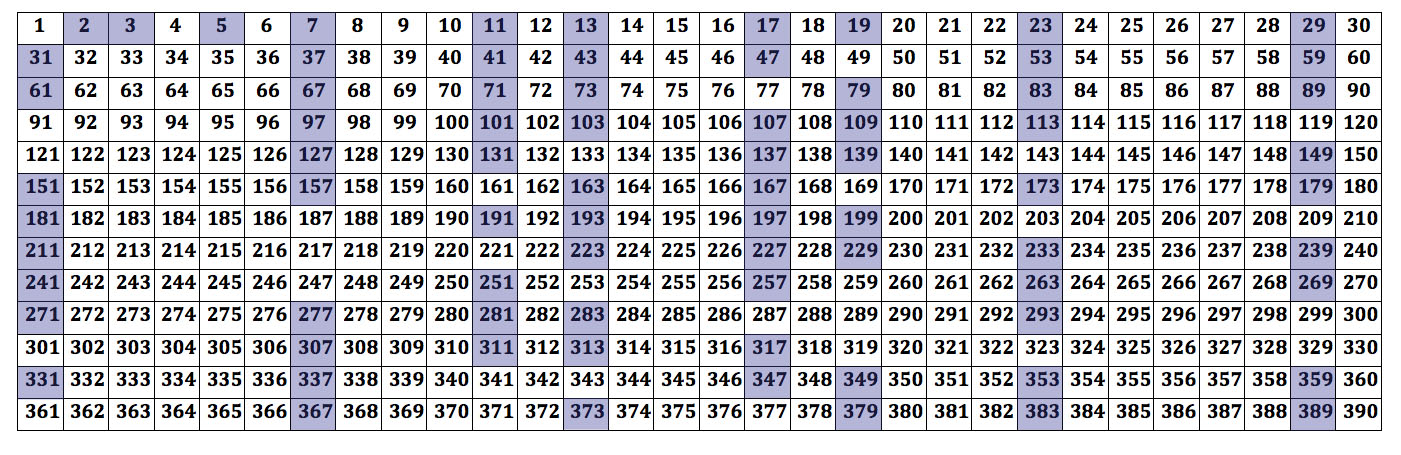
\includegraphics[scale=0.3]{figures/Numberrectangle-with-colored-primes_Irisprime.jpg}
\caption[Primzahlen unter den ersten 390 nat�rlichen Zahlen -- farblich markiert]
        {Primzahlen unter den ersten 390 nat�rlichen Zahlen -- farblich markiert\protect\footnotemark}
\label{Primes-in-a-390-integer-rechtangle-figure}
\end{center}
\end{figure}
\footnotetext{%
   Grafik von 
   \url{http://mathforum.org/mathimages/index.php/Image:Irisprime.jpg}, 30*13-Rechteck
   }

\begin{figure}[!hb]
\begin{center}
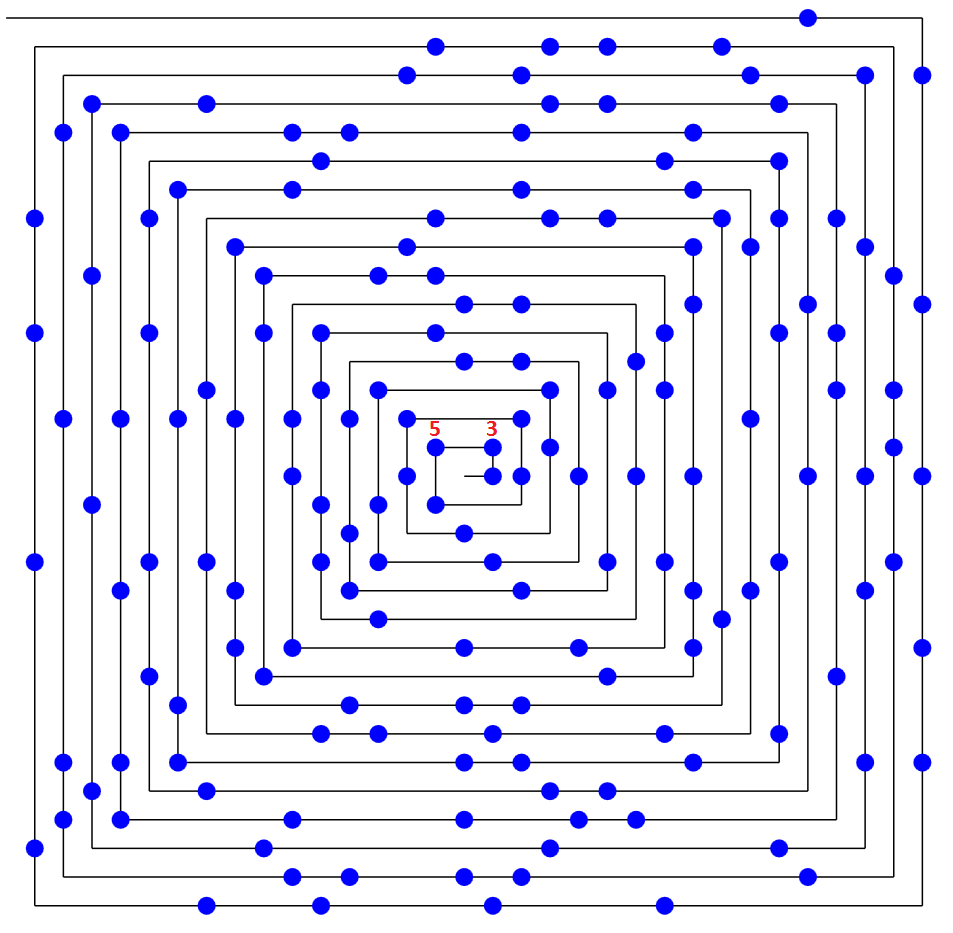
\includegraphics[scale=0.41]{figures/Ulam_spiral_via-CT2-within-1-999.png}
\caption[Primzahlen unter den ersten 999 nat�rlichen Zahlen -- als Ulam-Spirale]
        {Primzahlen unter den ersten 999 nat�rlichen Zahlen -- als Ulam-Spirale\protect\footnotemark}
\label{Primes-in-a-999-integer-ulam-spiral-figure}
\end{center}
\end{figure}
\footnotetext{%
   Grafik von CT2, Men� Kryptotutorien, Verteilung der Primzahlen, Ulam-Spirale; 32*32 Punkte
   }
%\newpage
\begin{figure}[!hb]
\begin{center}

\includegraphics{figures/Ulam_spiral_Wikipedia.png}
\caption[Primzahlen unter den ersten 4000 nat�rlichen Zahlen -- als Ulam-Spirale]
        {Primzahlen unter den ersten 4000 nat�rlichen Zahlen -- als Ulam-Spirale\protect\footnotemark}
\label{Primes-in-a-4000-integer-ulam-spiral-figure}
\end{center}
\end{figure}
\footnotetext{%
   Grafik von
   \url{http://mathforum.org/mathimages/index.php/Image:Ulam_spiral.png}, 200*200 Ulam-Spirale
   }



\newpage
\begin{satz}\label{thm-pz-sqr}
Jede ganze Zahl $m$ gr��er als $1$ besitzt einen kleinsten Teiler gr��er als $1$.
Dieser ist eine Primzahl $p$. Sofern $m$ nicht selbst eine Primzahl ist, gilt:
$p$ ist kleiner oder gleich der Quadratwurzel aus $m$.
\end{satz}

Aus den Primzahlen lassen sich alle ganzen Zahlen gr��er als $1$ zusammensetzen --- und das sogar in
einer eindeutigen Weise. Dies besagt der \textbf{1. Hauptsatz der Zahlentheorie} (= Hauptsatz der elementaren Zahlentheorie =
fundamental theorem of arithmetic = fundamental building block of all positive integers).\index{Zahlentheorie!Hauptsatz}

\begin{satz}\label{thm-pz-prod}
Jedes Element $n$ gr��er als $1$ der nat�rlichen Zahlen l�sst sich als Produkt
$n = p_1 \cdot p_2 \cdot \dots \cdot p_m$ von Primzahlen schreiben.
Sind zwei solche Zerlegungen
$$n =  p_1 \cdot p_2 \cdots p_m = p'_1 \cdot p'_2 \cdots p'_{m'}$$
gegeben, dann gilt nach eventuellem Umsortieren $\;m = m'\;$ und  f�r alle $i$:  $\;p_i = p'_i$. \\
($p_1, p_2, \dots, p_m$ nennt man die Primfaktoren\index{Primfaktor} von n).
\end{satz}

In anderen Worten: Jede nat�rliche Zahl au�er der $1$ l�sst sich auf genau eine Weise als Produkt von
Primzahlen schreiben, wenn man von der Reihenfolge der Faktoren absieht. Die Faktoren sind also
eindeutig (die {\em Expansion in Faktoren} ist eindeutig)!
Zum Beispiel ist
$$ 60 = 2 \cdot 2 \cdot 3 \cdot 5 = 2^2\cdot 3^1 \cdot 5^1 $$
Und das ist --- bis auf eine ver�nderte Reihenfolge der Faktoren
--- die einzige M�glichkeit, die Zahl $60$ in Primfaktoren zu
zerlegen. Wenn man nicht nur Primzahlen als Faktoren zul�sst,
gibt es mehrere M�glichkeiten der Zerlegung in Faktoren und die
\textbf{Eindeutigkeit} (\hypertarget{uniqueness}{uniqueness}) geht verloren:
$$ 60 = 1 \cdot 60 = 2 \cdot 30 = 4 \cdot 15 = 5 \cdot 12 =6 \cdot 10 = 2 \cdot 3 \cdot 10 =
        2 \cdot 5 \cdot 6 = 3 \cdot 4 \cdot 5 = \cdots . $$

Der folgende Absatz wendet sich eher an die mit der mathematischen Logik vertrauteren Menschen:
Der 1. Hauptsatz ist nur scheinbar selbstverst�ndlich\label{remFundTheoOfArithm}. Man kann viele andere Zahlenmengen
(ungleich der positiven ganzen Zahlen gr��er als 1) konstruieren, bei denen selbst eine Zerlegung in
die Primfaktoren dieser Mengen nicht eindeutig ist:
In der Menge $M = \{1, 5, 10, 15, 20, \cdots\}$ gibt es unter der Multiplikation kein Analogon zum Hauptsatz.
Die ersten f�nf Primzahlen dieser Folge sind $5, 10, 15, 20, 30$ (beachte: $10$ ist prim, da innerhalb
dieser Menge $5$ kein Teiler von $10$ ist --- das Ergebnis $2$ ist kein Element der gegebenen Grundmenge
$M$). Da in $M$ gilt:
$$ 100 = 5 \cdot 20 = 10 \cdot 10 $$
und sowohl $5, 10, 20$ Primzahlen dieser Menge sind, ist hier die Zerlegung in Primfaktoren nicht
eindeutig.

% --------------------------------------------------------------------------
\section{Wie viele Primzahlen gibt es?}

F�r die nat�rlichen Zahlen sind die Primzahlen vergleichbar mit den 
Elementen in der Chemie oder den Elementarteilchen in der Physik 
(vgl. \cite[S. 22]{pr:Blum1999}).

W�hrend es nur $92$ nat�rliche chemische Elemente gibt, ist die Anzahl 
der Primzahlen unbegrenzt.
Das wusste schon der Grieche \index{Euklid} Euklid\footnote{%
Euklid, griechischer Mathematiker des 4./3. Jahrhunderts vor Christus.
Wirkte an der Akademie in Alexandria und verfasste mit den
\glqq Elementen\grqq~ das bekannteste systematische Lehrbuch
der griechischen Mathematik.}
im dritten vorchristlichen Jahrhundert.
\begin{satz}[Euklid\footnote{Die �blich gewordene Benennung bedeutet nicht
unbedingt, dass Euklid der Entdecker des Satzes ist, da dieser
nicht bekannt ist. Der Satz wird bereits in Euklids \glqq Elementen\grqq ~(Buch IX, Satz 20) 
formuliert und bewiesen. Die dortige Formulierung ist insofern bemerkenswert,
als sie das Wort \glqq unendlich\grqq~ nicht verwendet; sie lautet
$$
O\acute{\iota}~\pi\varrho\tilde{\omega}\tau o \iota~\grave{\alpha}\varrho\iota\vartheta\mu o\grave{\iota}~
\pi\lambda\varepsilon\acute{\iota}o \upsilon\varsigma~\varepsilon\grave{\iota}\sigma\grave{\iota}~
\pi\alpha\nu\tau\grave{o}\varsigma~\tau o \tilde{\upsilon}~
\pi\varrho o \tau\varepsilon\vartheta\acute{\varepsilon}\nu\tau o \varsigma~
\pi\lambda\acute{\eta}\vartheta\ o \upsilon\varsigma~
\pi\varrho\acute{\omega}\tau\omega\nu~
\grave{\alpha}\varrho\iota\vartheta\mu\tilde{\omega}\nu,
$$
zu deutsch: Die Primzahlen sind mehr als jede vorgegebene Menge von Primzahlen.
}]\label{thm-pz-euklid}\hypertarget{thm-pz-euklid}{} % Ende der Fu�note
Die Folge der Primzahlen bricht nicht ab, es gibt also unendlich 
viele Primzahlen.
\end{satz}

Sein Beweis, dass es unendlich viele Primzahlen gibt, gilt bis heute als 
ein Glanzst�ck mathematischer �berlegung und Schlussfolgerung 
(\textbf{Widerspruchsbeweis}\index{Widerspruchsbeweis}). 
Er nahm an, es gebe nur endlich viele Primzahlen und damit eine gr��te
Primzahl. Daraus zog er solange logische Schl�sse, bis er auf einen
offensichtlichen Widerspruch stie�. Damit musste etwas falsch sein. Da 
sich in die Schlusskette kein Lapsus eingeschlichen hatte, konnte es nur 
die Annahme sein. Demnach musste es unendlich viele Primzahlen geben!\\

\hypertarget{euklid}{}
\index{Euklids Widerspruchsbeweis}\index{Widerspruchsbeweis}
% \paragraph*{Euklids Widerspruchsbeweis}
% Bei /paragraph den * angef�gt, damit es auch bei 4 Ebenen nicht im Inh.verzeichnis erscheint
% f�hrt die Argumentation wie folgt:
\begin{Beweis}{nach Euklid (Widerspruchsbeweis)\\}
{\bf Annahme:} \quad Es gibt {\em endlich} viele Primzahlen.
\\*[4pt] {\bf Schluss:} \quad Dann lassen sie sich auflisten $p_1
< p_2 < p_3 < \dots < p_n$, wobei $n$ f�r die (endliche) Anzahl
der Primzahlen steht. $p_n$ w�re also die gr��te Primzahl. Nun
betrachtet Euklid die Zahl $a = p_1 \cdot p_2 \cdots p_n +1$.
Diese Zahl kann keine Primzahl sein, da sie in unserer
Primzahlenliste nicht auftaucht. Also muss sie durch eine Primzahl
teilbar sein. D.h. es gibt eine nat�rliche Zahl $i$ zwischen $1$
und $n$, so dass $p_i$ die Zahl $a$ teilt. Nat�rlich teilt $p_i$
auch das Produkt $a-1 = p_1 \cdot p_2 \cdots p_n$, da $p_i$ ja ein
Faktor von $a-1$ ist. Da $ p_i $ die Zahlen $ a $ und $ a-1 $
teilt, teilt sie auch die Differenz dieser Zahlen. Daraus folgt:
$p_i$ teilt  $a - (a-1) = 1$. $p_i$ m�sste also $1$ teilen und
das ist unm�glich.\\*[4pt] 
{\bf Widerspruch}: \quad Unsere Annahme war falsch.\par
Also gibt es {\em unendlich} viele Primzahlen
(siehe \hyperlink{primhfk}{�bersicht unter \ref{s:primhfk}} �ber die
Anzahl von Primzahlen in verschiedenen Intervallen).
\end{Beweis} 

\par \vskip + 10pt

Wir erw�hnen hier auch noch eine andere, auf den ersten Blick 
�berraschende Tatsache, dass n�mlich in der Folge aller 
Primzahlen $p_1, p_2, \cdots $ L�cken von beliebig gro�er 
L�nge $n$ auftreten. Unter den $n$ aufeinanderfolgenden 
nat�rlichen Zahlen
$$ 
    (n+1)!+2, \cdots, (n+1)!+(n+1),
$$
ist keine eine Primzahl, da ja in ihnen der Reihe nach die 
Zahlen $2,\cdots, n+1$ als echte Teiler enthalten sind
(Dabei bedeutet $n!$ das Produkt der ersten $n$ nat�rlichen 
Zahlen, also $n!=n*(n-1)* \cdots *3*2*1$). 


% --------------------------------------------------------------------------
% --------------------------------------------------------------------------
\vskip + 20pt
\section{Die Suche nach sehr gro�en Primzahlen}
\label{search_for_very_big_primes}   % chap. 3.4

Die gr��ten heute bekannten Primzahlen haben mehrere
Millionen Stellen. Das ist unvorstellbar gro�. Die Anzahl
der Elementarteilchen im Universum wird auf eine \glqq nur\grqq\
$80$-stellige Zahl gesch�tzt \hyperlink{grosord}{(siehe
�bersicht unter \ref{s:grosord} �ber verschiedene Gr��enordnungen /
Dimensionen)}.


% --------------------------------------------------------------------------
\hypertarget{RecordPrimes}{}
\subsection{Die 20+ gr��ten bekannten Primzahlen (Stand Januar 2016)}  % Eyecatcher_neue-Mersenne
\index{Primzahlrekorde}
\label{RecordPrimes}

In der folgenden Tabelle sind die gr��ten, derzeit bekannten Primzahlen und
eine Beschreibung des jeweiligen Zahlentyps aufgef�hrt\footnote{%
Eine jeweils aktuelle Fassung findet sich im Internet
unter  \url{http://primes.utm.edu/largest.html},
unter  \url{http://primes.utm.edu/mersenne/index.html}, und
unter  \url{http://www.mersenne.org/primes/}.
}:
% Bsp-Meldungen
% - http://www.heise.de/newsticker/meldung/Neue-groesste-bekannte-Primzahl-mit-ueber-22-Millionen-Stellen-gefunden-3079127.html  20.01.2016
% - http://www.spiegel.de/wissenschaft/mensch/primzahlen-neue-rekord-zahl-mit-22-33-millionen-stellen-gefunden-a-1072883.html  20.1.16


%	10 & $1.372.930^{131.072}+1$ &   804.474 & 2003 & Verallg. Fermat\footnote{%
% $ 1.372.930^{131.072} + 1 = 1.372.930^{(2^{17})}+1 $ } \\

\index{Mersenne!Mersennezahl!verallgemeinerte} 
\index{Fermat!Fermatzahl!verallgemeinerte}

\begin{table}[ht]   % Vgl. http://primes.utm.edu/largest.html
\begin{center}
\begin{tabular}{|c|cccc|}
\hline \rule{0pt}{10pt}     % Eyecatcher_neue-Mersenne
 	& {\bf Definition} & {\bf Dezimalstellen} & {\bf Wann} & {\bf Beschreibung} \\
\hline \rule{0pt}{15pt} % Damit erreicht, dass die Exponenten nicht in die waagrechte Linie hineinragen.
        1  & $2^{74.207.281}-1$ & 22.338.618 & 2016 & Mersenne, 49. bekannte \\
	2  & $2^{57.885.161}-1$ & 17.425.170 & 2013 & Mersenne, 48. bekannte \\
	3  & $2^{43.112.609}-1$ & 12.978.189 & 2008 & Mersenne, 47. bekannte \\
	4  & $2^{42.643.801}-1$ & 12.837.064 & 2009 & Mersenne, 46. bekannte \\
	5  & $2^{37.156.667}-1$ & 11.185.272 & 2008 & Mersenne, 45. bekannte \\
	6  & $2^{32.582.657}-1$ &  9.808.358 & 2006 & Mersenne, M-44 \\
	7  & $2^{30.402.457}-1$ &  9.152.052 & 2005 & Mersenne, M-43 \\
	8  & $2^{25.964.951}-1$ &  7.816.230 & 2005 & Mersenne, M-42 \\
	9  & $2^{24.036.583}-1$ &  7.235.733 & 2004 & Mersenne, M-41 \\
	10 & $2^{20.996.011}-1$ &  6.320.430 & 2003 & Mersenne, M-40 \\
	11 & $2^{13.466.917}-1$ &  4.053.946 & 2001 & Mersenne, M-39 \\
	12 & $19.249 \cdot 2^{13.018.586}+1$ & 3.918.990 & 2007 & Verallgem. Mersenne\footnotemark \\
	13 & $27.653 \cdot 2^{9.167.433}+1$ & 2.759.677 & 2005 & Verallgem. Mersenne \\
	14 & $28.433 \cdot 2^{7.830.457}+1$ & 2.357.207 & 2004 & Verallgem. Mersenne \\
	15 & $2^{ 6.972.593}-1$ & 2.098.960 & 1999 & Mersenne, M-38 \\
	16 & $5.359 \cdot 2^{5.054.502}+1$ & 1.521.561 & 2003 & Verallgem. Mersenne \\
	17 & $4.847 \cdot 2^{3.321.063}+1$ & 999.744 & 2005 & Verallgem. Mersenne \\
	18 & $3 \cdot 2^{3.136.255}-1$ & 944.108 & 2007 & Verallgem. Mersenne \\
	19 & $2^{ 3.021.377}-1$ &   909.526 & 1998 & Mersenne, M-37 \\
	20 & $2^{ 2.976.221}-1$ &   895.932 & 1997 & Mersenne, M-36 \\
	21 & $222.361 \cdot 2^{2.854.840}+1$ & 859.398 & 2006 & Verallgem. Mersenne \\
	22 & $1.372.930^{131.072}+1$ &   804.474 & 2003 & Verallgem. Fermat\footnotemark \\
	23 & $1.361.244^{131.072}+1$ &   803.988 & 2004 & Verallgem. Fermat \\
	24 & $1.176.694^{131.072}+1$ &   795.695 & 2003 & Verallgem. Fermat \\
	25 & $342.673 \cdot 2^{2.639.439}-1$ & 794.556 & 2007 & Verallgem. Mersenne \\

\hline
\end{tabular}
\caption{Die 20+ gr��ten Primzahlen und ihr jeweiliger Zahlentyp
         (Stand Januar 2016)}    %  Eyecatcher_neue-Mersenne
\label{L_n_Largest_Known-Primes}
\end{center}
\end{table} 
\addtocounter{footnote}{-1}
\footnotetext{\index{Zahlen!Sierpinski}\index{Seventeen or Bust SoB}%
Diese Zahl wurde am 26.3.2007 im verteilt rechnenden Internet-Projekt
"`Seventeen or Bust"' (SoB) (\url{http://www.seventeenorbust.com})
% {\href{http://www.mersenne.org} {\tt http://www.mersenne.org}}
gefunden. Anders als das bekannte \hyperlink{GIMPS-project}{GIMPS-Projekt} (Kapitel~\ref{zahlentyp_mersenne}), das immer gr��ere der unendlich vielen Primzahlen aufsp�rt, k�nnte SoB aber irgendwann mal die gesetzte Aufgabe vollst�ndig erledigt haben.

Das SoB-Projekt versucht rechnerisch zu beweisen, dass die Zahl $k = 78.557$ die kleinste Sierpinski-Zahl ist (John Selfridge bewies 1962, dass $78.557$ eine Sierpinski-Zahl ist).

Der ber�hmte polnische Mathematiker Waclaw Sierpinski (1882 bis 1969) hatte im Jahre 1960 nachgewiesen, dass es unendlich viele ungerade nat�rliche Zahlen k gibt, die folgende Eigenschaft erf�llen: F�r jede Sierpinski-Zahl k gilt: S�mtliche Zahlen $N = k \cdot 2^{n}+1$ sind f�r alle nat�rlichen $n>=1$ zusammengesetzte Zahlen (Sierpinski's Composite Number Theorem, \url{http://mathworld.wolfram.com/SierpinskisCompositeNumberTheorem.html}).

Am Projektanfang im Jahre 2002 gab es noch 17 m�gliche Kandidaten $< 78557$ (daher der Name des Projekts "`Seventeen or Bust"'). Es reicht, wenn man ein einziges Gegenbeispiel findet, um einen Kandidaten k auszuschlie�en, also ein einziges $n>=1$ zu finden, so dass $N = k \cdot 2^{n}+1$ prim ist. Dass bei dieser Suche sehr gro�e Primzahlen gefunden werden, ist also eigentlich nur ein "`Nebenprodukt"' der Aufgabenstellung.

Vergleiche auch: 
\url{http://www.heise.de/newsticker/meldung/89582}.
} 
\addtocounter{footnote}{1}
\footnotetext{%
Verallgemeinerte Fermatzahl: $ 1.372.930^{131.072} + 1 = 1.372.930^{(2^{17})}+1 $ 
\index{Fermat!Fermatzahl!verallgemeinerte}
} 
%be_2005: footnetmark und footnotetext statt nur footnote (sonst sieht man nur
%         die Fussnoten-Nr., aber nicht den Text!
%be_2005: Erzwingen, dass die Abb. noch in diesem Kapitel !


Die gr��te bekannte Primzahl ist eine Mersenne-Primzahl.
Diese wurde vom \hyperlink{GIMPS-project}{GIMPS-Projekt}
(Kapitel~\ref{zahlentyp_mersenne}) gefunden.

Unter den gr��ten bekannten Primzahlen befinden sich au�erdem Zahlen
vom Typ \hyperlink{generalizedMersennenumbers}{verallgemeinerte Mersennezahl} 
(Kapitel~\ref{generalized-mersenne-no1})
und 
vom Typ \hyperlink{generalizedFermatprimes}{verallgemeinerte Fermatzahl} 
(Kapitel~\ref{generalized-fermat}).


% --------------------------------------------------------------------------
\hypertarget{MersenneNumbers01}{}
\subsection{Spezielle Zahlentypen -- Mersennezahlen und Mersenne-Primzahlen}
\label{zahlentyp_mersenne}
\index{Mersenne!Mersennezahl}

Nahezu alle bekannten riesig gro�en Primzahlen sind spezielle 
Kandidaten, sogenannte {\em Mersennezahlen}\footnote{%
Marin Mersenne, franz�sischer Priester und Mathematiker,
08.09.1588$-$01.09.1648.
\index{Mersenne, Marin}
}
der Form $2^p -1,$ wobei $p$ eine Primzahl ist.
Nicht alle Mersennezahlen sind prim:
$$
\begin{array}{cl}
2^2 - 1 = 3 & \Rightarrow {\rm prim} \\
2^3 - 1 = 7 & \Rightarrow {\rm prim} \\
2^5 - 1 = 31    & \Rightarrow {\rm prim} \\
2^7 - 1 = 127    & \Rightarrow {\rm prim} \\
2^{11} - 1 = 2.047 = 23 \cdot 89    & \Rightarrow  {\rm NICHT~prim} !
\end{array}
$$

\index{Zahlen!Mersennezahl}
\index{Mersenne!Mersennezahl} 
\index{Mersenne!Satz} 

Dass Mersennezahlen nicht immer Primzahlen (Mersenne-Primzahlen) sind, 
wusste auch schon Mersenne (siehe Exponent $p = 11$).
Eine Mersennezahl, die prim ist, wird Mersenne-Primzahl
\index{Mersenne!Mersenne-Primzahl} genannt.  \\

Dennoch ist ihm der interessante Zusammenhang zu verdanken, dass eine 
Zahl der Form $2^n-1$ keine Primzahl sein kann, wenn $n$ eine 
zusammengesetzte Zahl ist:

\begin{satz}[Mersenne]\label{thm-pz-mersenne}
  Wenn $2^n - 1$ eine Primzahl ist, dann folgt, $n$ ist ebenfalls eine 
  Primzahl (oder anders formuliert: $2^n - 1$ ist nur dann prim, 
  wenn $n$ prim ist).
\end{satz}

\begin{Beweis}{}
Der Beweis des Satzes von Mersenne kann durch Widerspruch
\index{Widerspruchsbeweis}
durchgef�hrt werden. Wir nehmen also an, dass es eine
zusammengesetzte nat�rliche Zahl $ n $ mit echter Zerlegung
$\; n=n_1 \cdot n_2 $
gibt, mit der Eigenschaft, dass $ 2^n -1 $ eine
Primzahl ist.

Wegen
\begin{eqnarray*}
(x^r-1)((x^r)^{s-1} + (x^r)^{s-2} + \cdots + x^r +1) & = &  ((x^r)^s + (x^r)^{s-1} + (x^r)^{s-2} + \cdots + x^r) \\
&  & -((x^r)^{s-1} + (x^r)^{s-2} + \cdots + x^r +1)  \\
& = & (x^r)^s -1 = x^{rs } -1,
\end{eqnarray*}
folgt
\[ 2^{n_1 n_2} - 1 = (2^{n_1} -1)((2^{n_1})^{n_2 -1} + (2^{n_1})^{n_2 -2} + \cdots + 2^{n_1} + 1). \]
Da $ 2^n - 1 $ eine Primzahl ist, muss einer der obigen beiden
Faktoren auf der rechte Seite gleich 1 sein. Dies kann nur dann
der Fall sein, wenn $ n_1 =1 $ oder $ n_2 =1$ ist. Dies ist aber
ein Widerspruch zu unserer Annahme. Deshalb ist unsere Annahme
falsch. Also gibt es keine zusammengesetzte Zahl $ n, $ so dass $
2^n -1 $ eine Primzahl ist.
\end{Beweis} 

\vskip + 5pt
\hypertarget{Mer-nums-not-always-prim}{}
Leider gilt dieser Satz nur in einer Richtung (die Umkehrung gilt
nicht, keine �quivalenz): das hei�t, dass es prime Exponenten gibt,
f�r die die zugeh�rige Mersennezahl {\bf nicht} prim ist (siehe das obige 
Beispiel $2^{11}-1, $ wo $11$ prim ist, aber $2^{11}-1$ nicht).

Mersenne behauptete, dass $2^{67}-1$ eine Primzahl ist. Auch zu
dieser Behauptung gibt es eine interessante mathematische Historie:
Zuerst dauerte es �ber 200 Jahre, bis \index{Lucas, Edouard}
Edouard Lucas (1842-1891) bewies, dass diese Zahl zusammengesetzt
ist. Er argumentierte aber indirekt und kannte keinen der
Faktoren. 1903 zeigte Cole\index{Cole, Frank Nelson}\footnote{%
Frank Nelson Cole, amerikanischer Mathematiker, 20.09.1861$-$26.05.1926.},
aus welchen Faktoren diese Primzahl besteht:
$$ 2^{67} -1 =147. 573. 952. 589. 676. 412. 927 = 193. 707. 721 \cdot 761. 838. 257. 287. $$
Er gestand, 20 Jahre an der Faktorisierung \index{Faktorisierung} (Zerlegung in Faktoren)%
\footnote{%
  Mit CT1\index{CrypTool 1} k�nnen Sie Zahlen auf folgende Weise 
  faktorisieren: Men� {\bf Einzelverfahren \textbackslash{} RSA-Kryptosystem 
  \textbackslash{} Faktorisieren einer Zahl}. \\
  In sinnvoller Zeit zerlegt CT1 mit dem Quadratischen Sieb (QS) auf einem Einzel-PC
  Zahlen bis 250 Bit L�nge.
  Zahlen gr��er als 1024 Bit werden zur Zeit von CT1 nicht angenommen.\\
  Mit CT2 kann man sowohl das QS als auch das GNFS (General Number Field Sieve)
  anwenden und die Berechnungen auf mehrere Rechner verteilen.\\
  Die aktuellen Faktorisierungsrekorde finden Sie in Kapitel
  \ref{nt:NoteFactorization}.
  \index{Faktorisierung!Faktorisierungsrekorde}
}
dieser 21-stelligen Dezimalzahl gearbeitet zu haben!

Dadurch, dass man bei den Exponenten der Mersennezahlen nicht alle 
nat�rlichen Zahlen verwendet, sondern nur die Primzahlen, engt man
den {\em Versuchsraum} deutlich ein. Die derzeit bekannten 
Mersenne-Primzahlen \index{Mersenne!Mersenne-Primzahl} gibt es 
f�r die Exponenten\footnote{%
Landon Curt Noll\index{Noll, Landon Curt} listet in einer Tabelle alle
bekannten Mersenne-Primzahlen samt Entdeckungsdatum und Wert in Zahlen-
und Wortform auf:
      \url{http://www.isthe.com/chongo/tech/math/prime/mersenne.html}\\
Siehe auch:
      \url{http://www.utm.edu/}.
                             }
$$
\begin{array}{c}
2, ~ 3, ~ 5, ~ 7, ~ 13, ~ 17, ~ 19, ~ 31, ~ 61, ~ 89, ~ 107, ~ 127, ~ 521, ~ 607, ~ 1.279, ~ 2.203, ~ 2.281, ~ 3.217, ~ 4.253, \\
4.423, ~9.689, ~ 9.941, ~ 11.213, ~ 19.937, ~ 21.701, ~ 23.207, ~ 44.497, ~ 86.243, ~ 110.503, ~ 132.049,\\
216.091, ~ 756.839, ~ 859.433, ~ 1.257.787, ~ 1.398.269, ~ 2.976.221, ~ 3.021.377, ~ 6.972.593,\\
 ~ 13.466.917, ~ 20.996.011, ~ 24.036.583, ~ 25.964.951, ~ 30.402.457, ~ 32.582.657,\\
 ~ 37.156.667, ~ 42.643.801, ~ 43.112.609.
% be_2005_UPDATEN_if-new-mersenne-prime-appears          ~ xxx.xxx.xxx.
\end{array}
$$
Damit sind heute    % Eyecatcher_neue-Mersenne
$49$                  % be_2005_UPDATEN_if-new-mersenne-prime-appears
Mersenne-Primzahlen\index{Primzahl!Mersenne}\index{Mersenne!Mersenne-Primzahl} 
bekannt.

\vskip +10 pt
Die $19$. Zahl mit dem Exponenten $4.253$ war die erste mit mindestens $1.000$
Stellen im Zehnersystem (der Mathematiker Samual \index{Yates,
Samual} Yates pr�gte daf�r den Ausdruck {\em titanische}
\index{Primzahl!titanische} Primzahl; sie wurde 1961 von Hurwitz
gefunden); die $27$. Zahl mit dem Exponenten $44.497$ war die
erste mit mindestens $10.000$ Stellen im Zehnersystem (Yates
pr�gte daf�r den Ausdruck \index{Primzahl!gigantische}  {\em
gigantische} Primzahl. Diese Bezeichnungen sind heute l�ngst
veraltet).

% \vskip - 4pt \noindent
% \begin{quote}
% (Der Supercomputerhersteller SGI Cray Research besch�ftigte nicht
% nur hervorragende Mathematiker, sondern benutzte die Primzahltests
% auch als Benchmarks f�r seine Maschinen.)
% \end{quote}

% \vspace{-10pt}
% \begin{itemize}
%  \item[] \url{http://reality.sgi.com/chongo/prime/prime_press.html}
% \end{itemize}


\vskip +10 pt
F�r die ersten 44  % be_2005_UPDATEN_if-new-mersenne-prime-appears % Eyecatcher_neue-Mersenne
Mersenne-Primzahlen wei� man inzwischen, dass diese Liste vollst�ndig ist. 
Die Exponenten bis zur 49.  % be_2005_UPDATEN_if-new-mersenne-prime-appears    % Eyecatcher_neue-Mersenne
bekannten Mersenne-Primzahl sind noch nicht vollst�ndig gepr�ft.\footnote{%
Den aktuellen Status der Pr�fung findet man auf der Seite:
      \url{http://www.mersenne.org/status.htm}.\\
Hinweise, wie man Zahlen auf ihre Primalit�t pr�fen kann, finden sich auch
in Kapitel \ref{primality_tests}, Primzahltests\index{Primzahltest}.      }


% be_2005_UPDATEN_if-new-mersenne-prime-appears    % Eyecatcher_neue-Mersenne
Inzwischen (Stand M�rz 2016) wurden alle primen Exponenten kleiner als
$ 35.183.273 $ getestet und nochmal gepr�ft\footnote{%
Siehe die Homepage des GIMPS-Projekts:
      \url{http://www.mersenne.org/report_milestones}.
                                  }:
somit k�nnen wir sicher sein, dass dies wirklich 
die 41. Mersenne-Primzahl ist und dass keine kleineren unentdeckten
Mersenne-Primzahlen existieren (es ist �blich, die Bezeichnung M-nn erst dann
zu verwenden, wenn die nn. bekannte Mersenne-Primzahl auch bewiesenerma�en die
nn. Mersenne-Primzahl ist).

\vskip +10 pt
Hier einige Beispiele mit ein paar mehr Details:

\vskip +10 pt
\paragraph*{M-37 -- Januar 1998} \index{Mersenne!Mersenne-Primzahl!M-37}\mbox{}

Die 37. Mersenne-Primzahl, $$2^{3.021.377} - 1 $$
wurde im Januar 1998 gefunden und hat
909.526 Stellen im Zehnersystem, was 33 Seiten in der FAZ entspricht!


\vskip +25 pt
\paragraph*{M-38 -- Juni 1999}\index{Mersenne!Mersenne-Primzahl!M-38}\mbox{}

Die 38. Mersenne-Primzahl, genannt M-38, $$ 2^{6.972.593} - 1 $$
wurde im Juni 1999 gefunden und hat $2.098.960$ Stellen im
Zehnersystem (das entspricht rund 77 Seiten in der FAZ).


\vskip +25 pt
\hypertarget{M-39}{}
\paragraph*{M-39 -- Dezember 2001}
\index{Mersenne!Mersenne-Primzahl!M-39}\mbox{}

Die 39. Mersenne-Primzahl, genannt M-39, $$2^{13.466.917}-1$$ 
wurde am 6.12.2001 bekanntgegeben: genau genommen war am 6.12.2001 
die Verifikation der am 14.11.2001 von dem kanadischen Studenten 
Michael Cameron gefundenen Primzahl abgeschlos"-sen.
Diese Zahl hat rund 4 Millionen Stellen (genau 4.053.946 Stellen). 
Allein zu ihrer Darstellung
$$
924947738006701322247758 \; \cdots  \; 1130073855470256259071
$$
br�uchte man in der FAZ knapp 200 Seiten.

%\vskip +25 pt
%\paragraph*{Mxxxxxxxxx -- Juni 2003 -- M-40 ?}
%\index{Mersenne!Mersenne-Primzahl!M-40}\mbox{}

%Als 40. Mersenne-Primzahl wurde die folgende Zahl gefunden (und schon als M-40
%bezeichnet, obwohl noch nicht sicher ist, ob es zwischen M-39 und
%Mxxxxxxxxxx nicht noch weitere Mersenne-Primzahlen gibt), $$2^{xx.xxx.xxx}-1$$ 
%Bekanntgegeben wurde sie am xx.06.2003: genau genommen war am xx.06.2003 
%die Verifikation der am 02.06.2003 von xxxxxxxxxxxxxxxx 
%gefundenen Primzahl abgeschlossen. 
%Initiator und Projektleiter George Woltman gibt eine gefundene Mersenne-Zahl
%erst bekannt, wenn eine Kontrollrechnung best�tigt, dass sie prim ist.
%Diese Zahl hat rund xxx Millionen Stellen (genau xx.xxx.xxx Dezimalstellen).
%Die erste Meldung in Deutsch dazu erschien 
%m.W. im Heise-Ticker\index{Heise-Ticker}:
%{\url{http://www.heise.de/newsticker/data/as-02.06.03-000/} }.




\vskip +25 pt
\paragraph*{GIMPS}\index{GIMPS}\mbox{}
\hypertarget{GIMPS-project}{}

Das GIMPS-Projekt\index{GIMPS} (Great Internet Mer"-senne-Prime Search)
wurde 1996 von George Woltman\index{Woltman, George} gegr�ndet, um neue 
gr��te Mersenne-Primzahlen zu finden ({\url{http://www.mersenne.org}}).
Genauere Erl�uterungen zu diesem Zahlentyp finden sich unter
\hyperlink{MersenneNumbers02}{Mersennezahlen} und 
\hyperlink{MersenneNumbers01}{Mersenne-Primzahlen}.

\begin{sloppypar}
Bisher hat das GIMPS-Projekt 15
   % be_2005_UPDATEN_if-new-mersenne-prime-appears    % Eyecatcher_neue-Mersenne
gr��te Mersenne-Primzahlen entdeckt, inklusive der gr��ten bekannten
Primzahl �berhaupt. 
\end{sloppypar}

Tabelle \ref{Primes_GIMPS-Primes_table-reference} enth�lt diese Mersenne
Rekord-Primzahlen.\footnote{%
Eine up-to-date gehaltene Version dieser Tabelle steht im Internet unter
     \url{http://www.mersenne.org/history.htm}.
}$^,$\footnote{%  Doppelfussnote
Bei jedem neuen Rekord, der gemeldet wird, beginnen in den einschl�gigen
Foren die immer gleichen, oft ironischen Diskussionen: Hat diese Forschung
einen tieferen Sinn? Lassen sich diese Ergebnisse f�r irgendwas verwenden?\\
Die Antwort ist, dass das noch unklar ist. Aber gerade das ist bei
Grundlagenforschung normal, dass man nicht sofort sieht, ob und wie es die
Menschheit voranbringt.
}

   % be_2005_UPDATEN_if-new-mersenne-prime-appears    % Eyecatcher_neue-Mersenne
\begin{table}[ht]
\begin{center}
\begin{tabular}{|cccc|}
\hline \rule{0pt}{10pt} 
	{\bf Definition} & {\bf Dezimalstellen} & {\bf Wann} & {\bf Wer} \\
\hline \rule{0pt}{15pt} 

	$2^{74.207.281}-1$ & 22.338.618 & 7. Januar 2016 & Curtis Cooper  \\
	$2^{57.885.161}-1$ & 17.425.170 & 25. Januar 2013 & Curtis Cooper  \\
	$2^{43.112.609}-1$ & 12.978.189 & 23. August 2008 & Edson Smith  \\
	$2^{42.643.801}-1$ & 12.837.064 & 12. April 2009 & Odd Magnar Strindmo \\
	$2^{37.156.667}-1$ & 11.185.272 & 6. September 2008 & Hans-Michael Elvenich \\

	$2^{32.582.657}-1$ &  9.808.358 & 4. September 2006 & Curtis Cooper/Steven Boone \\
	$2^{30.402.457}-1$ &  9.152.052 & 15. Dezember 2005 & Curtis Cooper/Steven Boone \\
	$2^{25.964.951}-1$ &  7.816.230 & 18. Februar 2005  & Martin Nowak \\
	$2^{24.036.583}-1$ &  7.235.733 & 15. Mai 2004      & Josh Findley     \\
	$2^{20.996.011}-1$ &  6.320.430 & 17. November 2003 & Michael Shafer   \\
	$2^{13.466.917}-1$ &  4.053.946 & 14. November 2001 & Michael Cameron  \\
	$2^{ 6.972.593}-1$ &  2.098.960 & 1. Juni 1999      & Nayan Hajratwala \\
	$2^{ 3.021.377}-1$ &    909.526 & 27. Januar 1998   & Roland Clarkson  \\
	$2^{ 2.976.221}-1$ &    895.932 & 24. August 1997   & Gordon Spence    \\
	$2^{ 1.398.269}-1$ &    420.921 & November 1996     & Joel Armengaud   \\
\hline
\end{tabular}
   % be_2005_UPDATEN_if-new-mersenne-prime-appears    % Eyecatcher_neue-Mersenne
\caption{Die gr��ten vom GIMPS-Projekt gefundenen Primzahlen (Stand Januar 2016)}
\label{Primes_GIMPS-Primes_table-reference}
\end{center}
\end{table} 

%be_2005: Erzwingen, dass die Abb. noch in diesem Kapitel !

Richard Crandall\index{Crandall, Richard} erfand den Transformations-Algorithmus,
der im GIMPS-Programm benutzt wird. George Woltman implementierte 
Crandall's Algorithmus in Maschinensprache, wodurch das Primzahlenprogramm 
eine vorher nicht da gewesene Effizienz erhielt. 
Diese Arbeit f�hrte zum GIMPS-Projekt.

Am 1. Juni 2003 wurde dem GIMPS-Server eine Zahl gemeldet, die evtl. die 40. 
Mersenne-Primzahl sein konnte. Diese wurde dann wie �blich �berpr�ft,
bevor sie ver�ffentlich werden sollte. 
Leider musste der Initiator und GIMPS-Projektleiter George Woltman Mitte Juni
melden, dass diese Zahl zusammengesetzt war (dies war die erste falsche
positive R�ckmeldung eines Clients an den Server in 7 Jahren).

Am GIMPS-Projekt beteiligen sich z.Zt. rund 130.000 
freiwillige Amateure und Experten, die ihre Rechner in das urspr�nglich von der 
Firma Entropia organisierte \glqq PrimeNet\grqq~ einbinden.






% --------------------------------------------------------------------------
\vskip +25 pt
\subsection{Wettbewerb der Electronic Frontier Foundation (EFF)}\index{EFF}
Angefacht wird diese Suche noch zus�tzlich durch einen Wettbewerb, den die
Non\-profit-Orga"-nisa"-tion EFF (Electronic Frontier Foundation) mit den
Mitteln eines unbekannten Spenders gestartet hat. Den Teilnehmern winken 
Gewinne im Gesamtwert von 500.000 USD, wenn sie die l�ngste Primzahl
finden. Dabei sucht der unbekannte Spender nicht nach dem schnellsten Rechner,
sondern er will auf die M�glichkeiten des {\em cooperative networking} 
aufmerksam machen: \\
{\url{http://www.eff.org/awards/coop}}

Der Entdecker von M-38 erhielt f�r die Entdeckung der ersten Primzahl
mit �ber 1 Million Dezimalstellen von der EFF eine Pr�mie von 50.000 USD. 

% be_2005_UPDATEN_if-new-mersenne-prime-appears
F�r die von 100.000 USD von der EFF f�r eine Primzahl mit mehr als
10 Millionen Dezimalstellen hat sich Edson Smith qualifiziert, der
im GIMPS-Projekt $ 2^{43.112.609}-1 $ fand.

Nach den Preisregeln der EFF sind dann als n�chste Stufe 150.000 US-Dollar
f�r eine Primzahl mit mehr als 100 Millionen Stellen ausgelobt.                         


Edouard Lucas\index{Lucas, Edouard} (1842-1891) hielt �ber 70 Jahre den 
Rekord der gr��ten bekannten Primzahl, indem er nachwies, dass 
$2^{127}-1$ prim ist. So lange wird wohl kein neuer Rekord mehr Bestand haben.


% --------------------------------------------------------------------------
\section[Primzahltests]{Primzahltests\footnotemark}
\footnotetext{%
    \index{ZT, Lernprogramm Zahlentheorie}%
    \index{Lernprogramm ZT}%
    In dem Lernprogramm {\bf ZT} k�nnen Sie den Fermat-Test und den
    Miller-Rabin-Test gef�hrt Schritt f�r Schritt anwenden: Siehe die 
    NT-Lern-Kapitel 3.2 und 3.3, Seiten 3-11/11.\\
    ZT k�nnen Sie in CT1\index{CrypTool 1} �ber das Men�
    {\bf Einzelverfahren \textbackslash{} Zahlentheorie interaktiv
    \textbackslash{} Lernprogramm f�r Zahlentheorie} aufrufen.
    Siehe auch Anhang \ref{s:appendix-Learn-NT}.\\
    Eine Visualisierung dieser Verfahren ist in CT2\index{CrypTool 2}
    in dem Tutorial \glqq {\bf World of Primes}\grqq~enthalten.
}
\label{primality_tests}   % chap. 3.5
\index{Primzahltest}

F�r die Anwendung sicherer Verschl�sselungsverfahren braucht man sehr gro�e
Primzahlen (im Bereich von $2^{2.048}$, das sind Zahlen im Zehnersystem mit
�ber $600$ Stellen!).

Sucht man nach den Primfaktoren, um zu entscheiden, ob eine Zahl prim ist,
dauert die Suche zu lange, wenn auch der kleinste Primfaktor riesig ist.
Die Zerlegung in Faktoren mittels rechnerischer systematischer Teilung oder
mit dem \hyperlink{SieveEratosthenes01}{Sieb des Eratosthenes} 
\index{Eratosthenes!Sieb} ist mit heutigen Computern anwendbar 
f�r Zahlen mit bis zu circa $20$ Stellen im Zehnersystem.
Die gr��te Zahl, die bisher in ihre beiden ann�hernd gleich gro�en
Primfaktoren zerlegt werden konnte, hatte 232 Stellen 
(vgl. \hyperlink{RSA-768-chap3}{RSA-768} in Kapitel~\ref{nt:NoteFactorization}).
% be_2005 Das ist eine gute Art zu referenzieren !!!!!!!!!!!!!!!

% be_2005_UPDATEN_if-new-factorization-record-appears

Ist aber etwas �ber die {\em Bauart} (spezielle Struktur) der fraglichen 
Zahl bekannt, gibt es sehr hochentwickelte Verfahren, die deutlich schneller
sind. Diese Verfahren beantworten nur die Primalit�tseigenschaft einer Zahl,
k�nnen aber nicht die Primfaktoren sehr gro�er zusammengesetzter Zahlen
bestimmen.

\hypertarget{FermatNumbers01}{}\label{FermatNumbers01}%
Fermat\footnote{%
Pierre de Fermat, franz�sischer Mathematiker, 17.8.1601 -- 12.1.1665.
\index{Fermat, Pierre}
}
\index{Fermat, Pierre} hatte im 17. Jahrhundert an Mersenne
\index{Mersenne, Marin} geschrieben, dass er vermute, 
dass alle Zahlen der Form $$ f(n) = 2^{2^n} + 1 $$ 
f�r alle ganzen Zahlen $ n \geq 0 $ prim seien 
(\hyperlink{FermatNumbers02}{siehe unten}, Kapitel~\ref{L-FermatNumbers02}).
\index{Zahlen!Fermatzahl}\index{Fermat!Fermatzahl}

Schon im 19. Jahrhundert wusste man, dass die $29$-stellige Zahl
$$ f(7) = 2^{2^7} + 1 $$
keine Primzahl ist. Aber erst 1970 fanden Morrison/Billhart ihre Zerlegung.
\label{F7Morrison}
\begin{eqnarray*}
f(7) & = & 340.282.366.920.938.463.463.374.607.431.768.211.457 \\
& = & 59. 649. 589. 127. 497. 217 \cdot  5.704.689.200.685.129.054.721
\end{eqnarray*}

Auch wenn sich Fermat bei seiner Vermutung irrte, so stammt in diesem
Zusammenhang von ihm doch ein sehr wichtiger Satz: Der (kleine)
Fermatsche Satz, den Fermat im Jahr 1640 aufstellte, ist der 
Ausgangspunkt vieler schneller Primzahltests 
(\hyperlink{KleinerSatzFermat-chap3}{siehe Kap.
\ref{Label_KleinerSatzFermat-chap3}}).

\hypertarget{KleinerSatzFermat-chap2}{}
\index{Fermat!kleiner Satz}
\begin{satz}[\glqq kleiner\grqq\ Fermat]\label{thm-pz-fermat1}
Sei $p$ eine Primzahl und $a$ eine beliebige ganze Zahl, dann gilt f�r
alle $a$ $$a^p \equiv a \; {\rm mod} \; p.$$
Eine alternative Formulierung lautet: \\
Sei $p$ eine Primzahl und $a$ eine beliebige ganze Zahl, die kein
Vielfaches von $p$ ist (also $a \not\equiv 0 \; {\rm mod} \; p$),
dann gilt $a^{p-1} \equiv 1 \; {\rm mod} \; p$.
\end{satz}

Wer mit dem Rechnen mit Resten (Modulo-Rechnung) nicht so vertraut ist, 
m�ge den Satz einfach so hinnehmen oder erst \hyperlink{Chapter_ElementaryNT}
{Kapitel \ref{Chapter_ElementaryNT} \glqq Einf�hrung
in die elementare Zahlentheorie mit Beispielen\grqq} lesen.
Wichtig ist, dass aus diesem Satz folgt, dass wenn
diese Gleichheit f�r irgendein ganzes $a$ nicht erf�llt ist, dann ist
$p$ keine Primzahl! Die Tests lassen sich (zum Beispiel f�r die erste
Formulierung) leicht mit der {\em Testbasis} $a = 2$ durchf�hren.

Damit hat man ein Kriterium f�r Nicht-Primzahlen, also einen negativen
Test, aber noch keinen Beweis, dass eine Zahl $a$ prim ist.
Leider gilt die Umkehrung zum Fermatschen Satz nicht, sonst h�tten
wir einen einfachen Beweis f�r die Primzahleigenschaft (man sagt auch,
man h�tte dann ein einfaches Primzahlkriterium).


\vskip +25 pt
\paragraph*{Pseudoprimzahlen}%
\index{Primzahl!Pseudoprimzahl}\index{Zahlen!Pseudoprimzahl}%
\hypertarget{HT-Pseudoprimenumber01}{}\label{L-Pseudoprimenumber01}%
\mbox{}
\vskip +10 pt
Zahlen n, die die Eigenschaft
$$ 2^n \equiv 2 \;{\rm mod}\; n $$
erf�llen, aber nicht prim sind, bezeichnet man als {\em Pseudoprimzahlen} 
(der Exponent n ist also keine Primzahl).
Die erste Pseudoprimzahl ist $$ 341 = 11 \cdot 31 .$$


\vskip +25 pt
\paragraph*{Carmichaelzahlen}%
\index{Zahlen!Carmichaelzahl}%
\hypertarget{HT-Carmichael-number01}{}\label{L-Carmichael-number01}%
\mbox{}
\vskip +10 pt
Es gibt Pseudoprimzahlen n, die den Fermat-Test 
$$ a^{n-1} \equiv 1 \;{\rm mod}\; n $$
mit allen Basen a, die teilerfremd zu n sind [$ gcd (a,n) = 1 $], bestehen,
obwohl die zu testenden Zahlen n nicht prim sind: Diese Zahlen hei�en
{\em Carmichaelzahlen}. Die erste ist
$$ 561 = 3 \cdot 11 \cdot 17 .$$

\begin{example}{: Die zu testende Zahl sei 561.}\\
Da $561 = 3 \cdot 11 \cdot 17$ ist, ergibt sich: \\
Die Testbedingung $a^{560} \;{\rm mod}\; 561 = 1$ \\
ist erf�llt f�r $a = 2, 4, 5, 7, \cdots $, \\
aber nicht f�r $a = 3, 6, 9, 11, 12, 15, 17, 18, 21, 22, \cdots$.\\
D.h. die Testbedingung muss nicht erf�llt sein, wenn die Basis ein
Vielfaches von 3, von 11 oder von 17 ist.\\
Der Test angewandt auf $a=3$ ergibt: $3^{560} \;{\rm mod}\; 561 = 375$. \\
Der Test angewandt auf $a=5$ ergibt: $5^{560} \;{\rm mod}\; 561 = 1$.
\end{example}

\vskip +25 pt
\paragraph*{Starke Pseudoprimzahlen}%
\index{Primzahl!starke Pseudoprimzahlen} \index{Zahlen!starke Pseudoprimzahl}%
\hypertarget{HT-Strongpseudoprimenumber01}{}\label{L-Strongpseudoprimenumber01}%
\mbox{}
\vskip +10 pt
Ein st�rkerer Test stammt von\index{Miller Gary L.}\index{Rabin, Michael O.}
Miller/Rabin\footnote{
1976 ver�ffentlichte Prof. Rabin einen effizienten probabilistischen
Primzahltest, der auf einem zahlentheoretischen Ergebnis von Prof. Miller aus
der Jahr davor basierte. \\
Prof. Miller arbeitete an der Carnegie-Mellon Universit�t, School of Computer
Science. Prof. Rabin, geboren 1931, arbeitete an der Harvard und Hebrew
Universit�t.
}%
: Dieser wird nur von sogenannten {\em starken Pseudoprimzahlen} bestanden. 
Wiederum gibt es starke Pseudoprimzahlen, die keine Primzahlen sind, aber
das passiert deutlich seltener als bei den (einfachen) Pseudoprimzahlen oder
bei den Carmichaelzahlen. Die kleinste starke Pseudoprimzahl zur Basis $2$ ist
$$ 15.841 = 7 \cdot 31 \cdot 73. $$
Testet man alle 4 Basen $2, 3, 5$ und $7$, so findet man bis $25 \cdot 10^9$
nur eine starke Pseudoprimzahl, also eine Zahl, die den Test besteht und doch keine Primzahl ist.

Weiterf�hrende Mathematik hinter dem Rabin-Test gibt dann die Wahrscheinlichkeit an, mit der die
untersuchte Zahl prim ist (solche Wahrscheinlichkeiten liegen heutzutage bei circa  $10^{-60}$).

Ausf�hrliche Beschreibungen zu Tests, um herauszufinden, ob eine Zahl
prim ist, finden sich zum Beispiel unter:
\vspace{-10pt}
\begin{itemize}
  \item[] \url{http://www.utm.edu/research/primes/mersenne.shtml} \\
          \url{http://www.utm.edu/research/primes/prove/index.html}
\end{itemize}



% --------------------------------------------------------------------------
\vskip +30 pt
\section{Spezial-Zahlentypen und die Suche nach einer Formel f�r
Primzahlen}\label{spezialzahlentypen}
\index{Primzahl!Formel}
Derzeit sind keine brauchbaren, offenen (also nicht rekursiven) Formeln bekannt, 
die nur Prim"-zahlen liefern (rekursiv bedeutet, dass zur Berechnung der Funktion
auf dieselbe Funktion in Abh�ngigkeit einer kleineren Variablen zugegriffen wird).
Die Mathematiker w�ren schon zufrieden, wenn sie eine Formel f�nden, die wohl 
L�cken l�sst (also nicht alle Primzahlen liefert), aber sonst keine
zusammengesetzten Zahlen (Nicht-Primzahlen) liefert.

Optimal w�re, man w�rde f�r das Argument $n$ sofort die $n$-te Primzahl 
bekommen, also f�r
$f(8) = 19\,$ oder f�r  $f(52) = 239$.

Ideen dazu finden sich in
\vspace{-10pt}
\begin{itemize}
  \item[] {\url{http://www.utm.edu/research/primes/notes/faq/p_n.html}}.
\end{itemize}


\hyperlink{ntePrimzahl}{Die Tabelle unter \ref{s:ntePrimzahl}} enth�lt 
die exakten Werte f�r die $n$-ten Primzahlen f�r ausgew�hlte $ n.$
\\

%  \glqq Primzahlformeln''
%  \glqq Primzahlformeln \grqq  (das Blank vor UND nach dem Text ist n�tig!
%        be_20050527: Aber dann war das Blank innerhalb der Hochkommata -> auch nicht gut
%  Fehlt es danach, wird der folgende Text direkt ohne Blank dahintergestellt!
F�r \glqq Primzahlformeln\grqq~werden meist ganz spezielle Zahlentypen
benutzt. Die folgende Auf"-z�hlung enth�lt die verbreitetesten Ans�tze 
f�r \glqq Primzahlformeln\grqq, und welche Kenntnisse wir �ber
sehr gro�e Folgeglieder haben: Konnte die Primalit�t bewiesen werden?
Wenn es zusammengesetzte Zahlen sind, konnten die Primfaktoren bestimmt werden?


% --------------------------------------------------------------------------
\vskip +10 pt
\hypertarget{MersenneNumbers02}{}
\subsection{Mersennezahlen \texorpdfstring{$f(n) = 2^n - 1$ f�r $ n $}{f(n) = 2\^{}n - 1 f�r n} prim}
    \index{Primzahl!Mersenne} \index{Mersenne!Mersenne-Primzahl}
    Wie \hyperlink{MersenneNumbers01}{oben} gesehen, liefert diese 
    Formel wohl relativ viele gro�e Primzahlen, aber es kommt -- wie 
    f�r $n=11$ [$f(n)=2.047$] -- immer wieder vor, dass das Ergebnis 
    auch bei primen Exponenten \hyperlink{Mer-nums-not-always-prim}{nicht}
    prim ist. \\
    Heute kennt man alle Mersenne-Primzahlen mit bis zu ca. 4.000.000 
    Dezimalstellen (\hyperlink{M-39}{M-39}
    \index{Mersenne!Mersenne-Primzahl!M-39}):
\vspace{-10pt}
\begin{itemize}
  \item[] {\url{http://perso.wanadoo.fr/yves.gallot/primes/index.html}}
\end{itemize}     % be_2005_UPDATEN_if-new-mersenne-prime-appears

% --------------------------------------------------------------------------
\vskip +10 pt
\subsection
    [Verallgemeinerte Mersennezahlen \texorpdfstring{$f(k,n) = k \cdot 2^n \pm 1$}{f(k,n) = k ... 2\^{}n +- 1} / Proth-Zahlen]
    {Verallgemeinerte Mersennezahlen 
    $f(k,n) = k \cdot 2^n \pm 1 $ f�r $ n $ prim und $ k $ kleine Primzahl
    / Proth-Zahlen\footnotemark}
    \footnotetext{%
       Diese wurden nach dem franz�sischen Landwirt Fran�ois Proth (1852-1879)
       benannt. Ber�hmter noch als die Proth-Primzahlen d�rfte das eng damit
       zusammenh�ngende Sierpinski-Problem\index{Zahlen!Sierpinski} sein,
       n�mlich Zahlen k zu finden, so dass $k*2^n+1$ zusammengesetzt ist f�r
       alle $n>0$. Siehe Tab. \ref{L_n_Largest_Known-Primes}.
    }
    \label{generalized-mersenne-no1}

    Diese erste Verallgemeinerung der 
    Mersennezahlen\index{Mersenne!Mersennezahl!verallgemeinerte} 
    erzeugt die sogenannten Proth-Zahlen\index{Zahlen!Proth-Zahl}.
    Daf�r gibt es (f�r kleine $k$) 
    ebenfalls sehr schnelle Primzahltests (vgl. \cite{pr:Knuth1981}).\\
    Praktisch ausf�hren l�sst sich das zum Beispiel mit der Software 
    Proths von Yves Gallot\index{Gallot, Yves}:
\vspace{-10pt}
\begin{itemize}
  \item[] {\url{http://www.prothsearch.net/index.html}}.
\end{itemize}


% --------------------------------------------------------------------------
\vskip +10 pt
\hypertarget{generalizedMersennenumbers}{}
\subsection
    [Verallgemeinerte Mersennezahlen \texorpdfstring{$ f(b,n) = b^n \pm 1$}{ f(b,n) = b\^{}n +- 1} / Cunningham-Projekt]
    {Verallgemeinerte Mersennezahlen
    $ f(b,n) = b^n \pm 1$ / Cunningham-Pro"-jekt}

    Dies ist eine zweite m�gliche Verallgemeinerung der 
    Mersennezahlen\index{Mersenne!Mersennezahl!verallgemeinerte}.
    Im \index{Cunningham-Projekt} \textbf{Cunningham-Pro"-jekt} werden die
    Faktoren aller zusammengesetzten Zahlen bestimmt, die sich in folgender
    Weise bilden:
    $$ f(b,n) = b^n \pm 1  \quad \mbox{f�r } b = 2, 3, 5, 6, 7, 10, 11, 12 $$
    ($b$ ist ungleich der Vielfachen von schon benutzten Basen wie $4, 8, 9$).

    Details hierzu finden sich unter:
\vspace{-10pt}
\begin{itemize}
  \item[] {\url{http://www.cerias.purdue.edu/homes/ssw/cun}}
\end{itemize}


% --------------------------------------------------------------------------
\vskip +10 pt
\hypertarget{FermatNumbers02}{}
\subsection[Fermatzahlen \texorpdfstring{$f(n) = 2^{2^n} + 1$}{f(n) = 2\^{}{2\^{}n} + 1}]
              {Fermatzahlen\footnotemark~$f(n) = 2^{2^n} + 1$}
    \footnotetext{%
       Die Fermatschen Primzahlen spielen unter
       anderem eine wichtige Rolle in der Kreisteilung. 
       Wie Gauss \index{Gauss, Carl Friedrich}
       bewiesen hat, ist das regul�re $p$-Eck f�r eine Primzahl $p>2$ dann
       und nur dann mit Zirkel und Lineal konstruierbar, wenn $p$ eine 
       Fermatsche Primzahl ist.
    }
    \label{L-FermatNumbers02}
    \index{Zahlen!Fermatzahl}\index{Fermat!Fermatzahl}
    \index{Primzahl!Fermat} \index{Fermat!Fermat-Primzahl}
    Wie \hyperlink{FermatNumbers01}{oben} in Kapitel~\ref{FermatNumbers01}
    erw�hnt, schrieb Fermat an 
    Mersenne, dass er vermutet, dass alle Zahlen dieser Form prim seien. 
    Diese Vermutung wurde jedoch von Euler (1732) widerlegt.
    Es gilt $641 | f(5)$.\footnote{%
    Erstaunlicherweise kann man mit Hilfe des Satzes von Fermat diese Zahl leicht finden (siehe z.B. 
    \cite[S. 176]{pr:Scheid1994})
    }
    
	       
%    Erstaunlicherweise w�re es f�r ihn m�glich gewesen, mit dem auf 
%    seinem kleinen Satz beruhenden negativen Primzahltest f�r $n=5$ ein 
%    positives Ergebnis zu erhalten.
$$
\begin{array}{lll}
f(0) = 2^{2^0} + 1  = 2^1 + 1 & = 3 &   \mapsto {\rm ~prim}  \\
f(1) = 2^{2^1} + 1  = 2^2 + 1 & = 5 &   \mapsto {\rm ~prim}  \\
f(2) = 2^{2^2} + 1  = 2^4 + 1 & = 17 &  \mapsto {\rm ~prim}  \\
f(3) = 2^{2^3} + 1  = 2^8 + 1 & = 257 & \mapsto {\rm ~prim}  \\
f(4) = 2^{2^4} + 1  = 2^{16} + 1 &  = 65.537 &  \mapsto {\rm ~prim}  \\
f(5) = 2^{2^5} + 1  = 2^{32} + 1 &  = 4.294.967.297 = 641 \cdot
6.700.417 &  \mapsto {\rm ~NICHT~prim} !\\
f(6) = 2^{2^6} + 1  = 2^{64} + 1 &  = 18.446.744.073.709.551.617 \\
                                 &  = 274.177 \cdot 67.280.421.310.721  
																 & \mapsto {\rm ~NICHT~prim} ! \\
f(7) = 2^{2^7} + 1  = 2^{128} + 1 & = \mbox{(siehe Seite~\pageref{F7Morrison})}  
																 & \mapsto {\rm ~NICHT~prim} !
															
\end{array}
$$

    Innerhalb des Projektes \glqq Distributed Search for Fermat Number
    Dividers\grqq, das von Leonid Durman angeboten wird, gibt es ebenfalls
    Fortschritte beim Finden von neuen Primzahl-Riesen
    ({\url{http://www.fermatsearch.org/}}  --  diese Webseite hat 
    Verkn�pfungen zu Seiten in russisch, italienisch und deutsch).
    \begin{sloppypar}
    Die entdeckten Faktoren k�nnen sowohl zusammengesetzte nat�r"-liche als
    auch prime nat�rliche Zahlen sein.
    \end{sloppypar}
     
    Am 22. Februar 2003 entdeckte John Cosgrave
    \begin{itemize} 
     \item die gr��te bis dahin bekannte zusammengesetzte Fermatzahl und
     \item die gr��te bis dahin bekannte prime nicht-einfache Mersennezahl
           mit 645.817 Dezimalstellen.
    \end{itemize}


    Die Fermatzahl
    $$ f(2.145.351) = 2^{(2^{2.145.351})} + 1 $$ 
    ist teilbar durch die Primzahl
    $$ p = 3*2^{2.145.353} + 1 $$ \\
    Diese Primzahl p war damals die gr��te bis dahin bekannte prime 
    verallgemeinerte Mersennezahl\index{Mersenne!Mersennezahl!verallgemeinerte}
    und die 5.-gr��te damals bekannte Primzahl �berhaupt. 

    Zu diesem Erfolg trugen bei: NewPGen von Paul Jobling's, PRP von 
    George Woltman's, Proth von Yves Gallot's Programm\index{Gallot, Yves} und
    die Proth-Gallot-Gruppe am St. Patrick's College, Dublin.

    Weitere Details finden sich unter
    \vspace{-10pt}
    \begin{itemize}
      \item[] \url{http://www.fermatsearch.org/history/cosgrave_record.htm/}
    \end{itemize}


%    ({\url{http://perso.wanadoo.fr/yves.gallot/primes/index.html} }).
% M.E. ist die Zahl auf seiner Webseite zu gro�, da M-39 "nur" 4 Mio. Stellen hat !
%    Heute kennt man alle Fermatschen Primzahlen mit bis zu 2.000.000.000 ???
%    Dezimalstellen. \\




% --------------------------------------------------------------------------
\vskip +10 pt
\hypertarget{generalizedFermatprimes}{}    %be_2005 Eigentlich sind es "Zahlen", nicht nur "Primes" !
\subsection
    [Verallgemeinerte Fermatzahlen \texorpdfstring{$f(b,n) = b^{2^n} + 1$}{f(b,n) = b\^{}{2\^{}n} + 1}]
    {Verallgemeinerte Fermatzahlen\footnotemark~$f(b,n) = b^{2^n} + 1$}
    \footnotetext{%
      Hier ist die Basis b nicht notwendigerweise 2.
      Noch allgemeiner w�re:  $f(b,c,n) = b^{c^n} \pm 1$
    }
\label{generalized-fermat}
\index{Fermat!Fermatzahl!verallgemeinerte}
    Verallgemeinerte Fermatzahlen kommen h�ufiger vor als Mersennezahlen
    gleicher Gr��e, so dass wahrscheinlich noch viele gefunden werden 
    k�nnen, die die gro�en L�cken zwischen den Mersenne-Primzahlen 
    verkleinern.
    Fortschritte in der Zahlentheorie haben es erm�g"-licht, dass Zahlen,
    deren Repr�sentation nicht auf eine Basis von 2 beschr�nkt ist, 
    nun mit fast der gleichen Geschwindigkeit wie Mersennezahlen getestet
    werden k�nnen.
    
    Yves Gallot\index{Gallot, Yves} schrieb das Programm Proth.exe zur 
    Untersuchung verallgemeinerter Fermat"-zahlen.
    
    Mit diesem Programm fand Michael Angel am 16. Februar 2003 eine
    prime verallgemeinerte Fermatzahl mit 628.808 Dezimalstellen, 
    die zum damaligen Zeitpunkt zur 5.-gr��ten bis dahin bekannten
    Primzahl wurde:
    $$ b^{2^{17}} + 1  =  62.722^{131.072} + 1. $$ 

    Weitere Details finden sich unter
    \vspace{-10pt}
    \begin{itemize}
      \item[] \url{http://primes.utm.edu/top20/page.php?id=12} 
    \end{itemize}




% --------------------------------------------------------------------------
\vskip +10 pt
\subsection{Carmichaelzahlen}\index{Zahlen!Carmichaelzahl}
Wie \hyperlink{HT-Carmichael-number01}{oben} in
Kapitel~\ref{L-Carmichael-number01} erw�hnt,
sind nicht alle Carmichaelzahlen prim.


% --------------------------------------------------------------------------
\vskip +10 pt
\subsection{Pseudoprimzahlen}
\index{Primzahl!Pseudoprimzahl}\index{Zahlen!Pseudoprimzahl}
Siehe \hyperlink{HT-Pseudoprimenumber01}{oben} in
Kapitel~\ref{L-Pseudoprimenumber01}.


% --------------------------------------------------------------------------
\vskip +10 pt
\subsection{Starke Pseudoprimzahlen}
\index{Primzahl!starke Pseudoprimzahlen} \index{Zahlen!starke Pseudoprimzahl}
Siehe \hyperlink{HT-Strongpseudoprimenumber01}{oben} in
Kapitel~\ref{L-Strongpseudoprimenumber01}.



% --------------------------------------------------------------------------
\vskip +10 pt
\subsection
    [Idee aufgrund von Euklids Beweis \texorpdfstring{$p_1 \cdot p_2 \cdots p_n +1$}{p\_1 ... p\_2 ... p\_n +1}]
    {Idee aufgrund von Euklids Beweis $p_1 \cdot p_2 \cdots p_n +1$}
Diese Idee entstammt \hyperlink{thm-pz-euklid}{Euklids Beweis}, dass es
unendlich viele Primzahlen gibt.
$$
\begin{array}{lll}
2{\cdot}3 +1 &      = 7 &          \mapsto {\rm ~prim} \\
2{\cdot}3{\cdot}5 +1 &      = 31    &      \mapsto {\rm ~prim} \\
2{\cdot}3{\cdot}5{\cdot}7 +1 &      = 211   &      \mapsto {\rm ~prim} \\
2{\cdot}3{\cdots}11 +1 &        = 2311  &      \mapsto {\rm ~prim} \\
2\cdot3 \cdots 13 +1 &  = 59 \cdot 509 &    \mapsto {\rm ~NICHT~prim} ! \\
2\cdot3 \cdots 17 +1 &  = 19 \cdot 97 \cdot 277 &   \mapsto {\rm ~NICHT~prim} ! \\
\end{array} 
$$


% --------------------------------------------------------------------------
\vskip +10 pt
\subsection{Wie zuvor, nur \texorpdfstring{$-1$ statt $+1$: $p_1 \cdot p_2 \cdots p_n -1$}{-1 statt +1: p\_1 ... p\_2 ... p\_n -1}}
$$
 \begin{array}{lll}
2\cdot 3 -1     &   = 5 &   \mapsto {\rm ~prim} \\
2\cdot 3 \cdot  5  -1   &   = 29 &  \mapsto {\rm ~prim} \\
2\cdot 3 \cdots 7  -1   &   = 11 \cdot 19 & \mapsto {\rm ~NICHT~prim} ! \\
2\cdot 3 \cdots 11 -1   &   = 2309 &    \mapsto {\rm ~prim} \\
2\cdot 3 \cdots 13 -1  &    = 30029 &   \mapsto {\rm ~prim} \\
2\cdot 3 \cdots 17 -1    &  = 61 \cdot 8369 &   \mapsto {\rm ~NICHT~prim!}
\end{array}
$$


% --------------------------------------------------------------------------
\vskip +10 pt
\subsection[Euklidzahlen \texorpdfstring{$e_n = e_0 \cdot e_1 \cdots e_{n-1} + 1$}{e\_n = e\_0 ... e\_1 ... e\_n-1 + 1}]
              {Euklidzahlen $e_n = e_0 \cdot e_1 \cdots e_{n-1} + 1$  
	       mit $ n \geq 1 $ und $ e_0 := 1 $}
%	       mit $n$ gr��er oder gleich $1$ und $e_0 := 1$}
    \index{Euklidzahlen}
    $e_{n-1}$ ist nicht die $(n-1)$-te Primzahl, sondern die zuvor hier 
    gefundene Zahl.
    Diese Formel ist leider nicht offen, sondern rekursiv.
    Die Folge startet mit
$$
\begin{array}{lll}
e_1 = 1 + 1 &   = 2 &   \mapsto {\rm ~prim} \\
e_2 = e_1 + 1   &   = 3 &   \mapsto {\rm ~prim} \\
e_3 = e_1 \cdot e_2 + 1 &   = 7 &   \mapsto {\rm ~prim} \\
e_4 = e_1 \cdot e_2 \cdot e_3 + 1 & = 43 &  \mapsto {\rm ~prim} \\
e_5 = e_1 \cdot e_2 \cdots e_4 + 1 &    = 13 \cdot 139 &    \mapsto {\rm ~NICHT~prim} ! \\
e_6 = e_1 \cdot e_2 \cdots e_5 + 1 &    = 3.263.443 &   \mapsto {\rm ~prim} \\
e_7 = e_1 \cdot e_2 \cdots e_6 + 1 &    = 547 \cdot 607 \cdot 1.033 \cdot 31.051 & \mapsto {\rm ~NICHT~prim} ! \\
e_8 = e_1 \cdot e_2 \cdots e_7 + 1 &    = 29.881\cdot 67.003 \cdot 9.119.521 \cdot 6.212.157.481 & \mapsto {\rm ~NICHT~prim} !
\end{array}
$$

\noindent Auch $e_9, \cdots, e_{17}$ sind zusammengesetzt, so dass dies auch
keine brauchbare Primzahlformel ist.

\begin{remark}{:}\\
Das Besondere an diesen Zahlen ist, dass sie jeweils paarweise
keinen gemeinsamen Teiler au�er $1$ haben\footnote{%
Dies kann leicht gezeigt werden mit Hilfe der Rechenregel f�r den
{\em gr��ten gemeinsamen Teiler ggT} \\
mit $ggT(a,b) = ggT(b-\lfloor b/a\rfloor \cdot a, a)$.\\ 
Es gilt f�r $i<j$: \\
$ggT(e_i,e_j) \le ggT(e_1 \cdots e_i \cdots e_{j-1}, e_j) = ggT(e_j - e_1 \cdots e_i \cdots e_{j-1}, e_1 \cdots e_i \cdots e_{j-1}) 
= ggT(1, e_1 \cdots e_i \cdots e_{j-1}) = 1$.\\
Siehe Seite \pageref{nt:NumberTheory_Appendix_GCD}.  %KORR_NumberTheory_Appendix_A mk56_ok_now
}, sie sind also%
\index{Primzahl!relative}\index{Zahlen!relativ prim} {\em relativ zueinander prim}.
\end{remark}

% --------------------------------------------------------------------------
% f(40) hier und f(80) im folgenden Kapitel nach Hinweis von Erik Berger korr. (2005-05)
\vskip +10 pt
\subsection{\texorpdfstring{$f(n) = n^2 + n + 41$}{f(n) = n\^{}2 + n + 41}}
\label{L-Polynomfunktion01-41}
   Diese Folge hat einen sehr {\em erfolgversprechenden} Anfang,
   aber das ist noch lange kein Beweis.
$$
\begin{array}{lll}
f(0) = 41 & &  \mapsto {\rm ~prim} \\
f(1) = 43 & &  \mapsto {\rm ~prim} \\
f(2) = 47 & &  \mapsto {\rm ~prim} \\
f(3) = 53 & &  \mapsto {\rm ~prim} \\
f(4) = 61 & &  \mapsto {\rm ~prim} \\
f(5) = 71 & &  \mapsto {\rm ~prim} \\
f(6) = 83 & &  \mapsto {\rm ~prim} \\
f(7) = 97 & &  \mapsto {\rm ~prim} \\
\vdots \\
f(33) = 1.163 & & \mapsto {\rm ~prim} \\
f(34) = 1.231 & & \mapsto {\rm ~prim} \\
f(35) = 1.301 & & \mapsto {\rm ~prim} \\
f(36) = 1.373 & & \mapsto {\rm ~prim} \\
f(37) = 1.447 & & \mapsto {\rm ~prim} \\
f(38) = 1.523 & & \mapsto {\rm ~prim} \\
f(39) = 1.601 & & \mapsto {\rm ~prim} \\
f(40) = 1681 & = 41 \cdot 41 &  \mapsto {\rm ~NICHT~prim}! \\
f(41) = 1763 & = 41 \cdot 43 &   \mapsto {\rm ~NICHT~prim}! \\
\end{array}
$$
        Die ersten $40$ Werte sind Primzahlen (diese haben die auffallende
        Regelm��igkeit, dass ihr Abstand beginnend mit dem Abstand $2$ 
        jeweils um $2$ w�chst), aber der $41$. und der $42$. Wert
        sind keine Primzahlen.
        Dass $f(41)$ keine Primzahl sein kann, l�sst sich leicht �berlegen:
        $f(41) = 41^2 + 41 + 41 = 41 (41 + 1 + 1) = 41 \cdot 43$.



% --------------------------------------------------------------------------
\vskip +10 pt
\subsection{\texorpdfstring{$f(n) = n^2 - 79 \cdot n + 1.601$}{f(n) = n\^{}2 - 79 ... n + 1.601}}
\label{L-Polynomfunktion02-1601}   \label{SrcPrimArith1}
   Diese Funktion liefert f�r die Werte $n=0$ bis $n=79$ stets
   Primzahlwerte.\footnote{%
   In Kapitel~\ref{primes:_Appendix_Sage-Samples},
   \glqq \nameref{primes:_Appendix_Sage-Samples}\grqq~finden Sie den
   Quellcode zur Berechnung der Tabelle mit SageMath\index{SageMath}.}
   Leider ergibt $f(80) = 1.681 = 11 \cdot 151$ keine Primzahl. Bis heute
   kennt man keine Funktion, die mehr aufeinanderfolgende Primzahlen annimmt.
   Andererseits kommt jede Primzahl doppelt vor (erst in der absteigenden,
   dann in der aufsteigenden Folge), so dass sie insgesamt genau 40 
   verschiedene Primzahlwerte in Folge liefert (Es sind dieselben wie die, die
   die Funktion aus Kapitel~\ref{L-Polynomfunktion01-41} liefert)\footnote{%
   Ein weiteres quadratisches Polynom, das dieselben Primzahlen liefert, ist: 
   $f(n) = n^2 - 9 \cdot n + 61$.\\ Unter den ersten 1000 Folgegliedern dieser
   Funktion sind �ber 50\% prim (vgl. Kapitel~\ref{primes:_Appendix_Sage-Samples},
   \glqq \nameref{primes:_Appendix_Sage-Samples}\grqq).}.

$$
\begin{array}{| ll       || ll |}
\hline
f(0)  = 1.601 & \mapsto {\rm ~prim}   &   f(26) =   223 & \mapsto {\rm ~prim} \\
f(1)  = 1.523 & \mapsto {\rm ~prim}   &   f(27) =   197 & \mapsto {\rm ~prim} \\
f(2)  = 1.447 & \mapsto {\rm ~prim}   &   f(28) =   173 & \mapsto {\rm ~prim} \\
f(3)  = 1.373 & \mapsto {\rm ~prim}   &   f(29) =   151 & \mapsto {\rm ~prim} \\
f(4)  = 1.301 & \mapsto {\rm ~prim}   &   f(30) =   131 & \mapsto {\rm ~prim} \\
f(5)  = 1.231 & \mapsto {\rm ~prim}   &   f(31) =   113 & \mapsto {\rm ~prim} \\
f(6)  = 1.163 & \mapsto {\rm ~prim}   &   f(32) =    97 & \mapsto {\rm ~prim} \\
f(7)  = 1.097 & \mapsto {\rm ~prim}   &   f(33) =    83 & \mapsto {\rm ~prim} \\
f(8)  = 1.033 & \mapsto {\rm ~prim}   &   f(34) =    71 & \mapsto {\rm ~prim} \\
f(9)  =   971 & \mapsto {\rm ~prim}   &   f(35) =    61 & \mapsto {\rm ~prim} \\
f(10) =   911 & \mapsto {\rm ~prim}   &   f(36) =    53 & \mapsto {\rm ~prim} \\
f(11) =   853 & \mapsto {\rm ~prim}   &   f(37) =    47 & \mapsto {\rm ~prim} \\
f(12) =   797 & \mapsto {\rm ~prim}   &   f(38) =    43 & \mapsto {\rm ~prim} \\
f(13) =   743 & \mapsto {\rm ~prim}   &   f(39) =    41 & \mapsto {\rm ~prim} \\
f(14) =   691 & \mapsto {\rm ~prim}   &   f(40) =    41 & \mapsto {\rm ~prim} \\              
f(15) =   641 & \mapsto {\rm ~prim}   &   f(41) =    43 & \mapsto {\rm ~prim} \\              
f(16) =   593 & \mapsto {\rm ~prim}   &   f(42) =    47 & \mapsto {\rm ~prim} \\              
f(17) =   547 & \mapsto {\rm ~prim}   &   f(43) =    53 & \mapsto {\rm ~prim} \\              
f(18) =   503 & \mapsto {\rm ~prim}   &   \cdots  &  \\                                       
f(19) =   461 & \mapsto {\rm ~prim}   &   f(77) = 1.447 & \mapsto {\rm ~prim} \\             
f(20) =   421 & \mapsto {\rm ~prim}   &   f(78) = 1.523 & \mapsto {\rm ~prim} \\             
f(21) =   383 & \mapsto {\rm ~prim}   &   f(79) = 1.601 & \mapsto {\rm ~prim} \\             
f(22) =   347 & \mapsto {\rm ~prim}   &   f(80) = 41 \cdot 41 & \mapsto {\rm ~NICHT~prim!} \\
f(21) =   383 & \mapsto {\rm ~prim}   &   f(81) = 41 \cdot 43 & \mapsto {\rm ~NICHT~prim!} \\ 
f(22) =   347 & \mapsto {\rm ~prim}   &   f(82) = 1.847 & \mapsto {\rm ~prim} \\             
f(23) =   313 & \mapsto {\rm ~prim}   &   f(83) = 1.933 & \mapsto {\rm ~prim} \\              
f(24) =   281 & \mapsto {\rm ~prim}   &   f(84) = 43 \cdot 47 &  \mapsto {\rm ~NICHT~prim!} \\
f(25) =   251 & \mapsto {\rm ~prim}   &   & \\
\hline
\end{array}
$$



% --------------------------------------------------------------------------
\vskip +20 pt
\subsection[Polynomfunktionen
    \texorpdfstring{$f(x) = a_n x^n + a_{n-1}x^{n-1} + \cdots + a_1 x^1 + a_0$}
                   {f(x) = a\_n x\^{}n + a\_n-1 x\^{}n-1 + ... + a\_1 x\^{}1 + a\_0}]
    {Polynomfunktionen
    $f(x) = a_n x^n + a_{n-1}x^{n-1} + \cdots + a_1 x^1 + a_0$  
    ($a_i$ aus ${\mathbb Z}$, $n \geq 1$)}\index{Polynom}
%\item Polynomfunktionen} $f(x) = a_n x^n + a_{n-1}x^{n-1} + 
%\cdots + a_1 x^1 + a_0$  ($a_i$ aus ${\mathbb Z}$, $n \geq 1$):

    Es existiert kein solches Polynom, das f�r alle $x$ aus ${\mathbb Z}$ 
    ausschlie�lich Primzahlwerte annimmt.
    Zum Beweis sei auf \cite[S. 83 f.]{pr:Padberg1996}, verwiesen, wo sich auch
    weitere Details zu Primzahl"-for"-meln finden.

    Damit ist es hoffnungslos, weiter nach Formeln (Funktionen) wie in
    Kapitel~\ref{L-Polynomfunktion01-41} oder 
    Kapitel~\ref{L-Polynomfunktion02-1601} zu suchen.

    

% --------------------------------------------------------------------------
\vskip +10 pt
\subsection[Catalans Mersenne-Vermutung]{Catalans Mersenne-Vermutung\footnotemark}
    \footnotetext{%
Eugene Charles Catalan, belgischer Mathematiker, 30.5.1814$-$14.2.1894.\\
Nach ihm sind auch die sogenannten {\em Catalanzahlen}
$A(n) = (1 / (n+1) ) * (2n)! / (n!)^2$ \\
$=  1, 2, 5, 14, 42, 132, 429, 1.430, 
4.862, 16.796, 58.786, 208.012, 742.900, 2.674.440, 9.694.845, ... $
benannt.
    }
\nopagebreak
Catalan\index{Catalan, Eugene}\index{Zahlen!Catalanzahl}
�u�erte die Vermutung\footnote{%
Siehe \url{http://www.utm.edu/research/primes/mersenne.shtml}
           unter "`Conjectures and Unsolved Problems"'.
         }, dass $ C_4 \;$ und jede weitere Zahl dieser Folge eine Primzahl ist:
$$
\begin{array}{l}
C_0 = 2, \\
C_1 = 2^{C_0} - 1,  \\
C_2 = 2^{C_1} - 1,  \\
C_3 = 2^{C_2} - 1, \\
C_4 = 2^{C_3} - 1, \cdots \\
\end{array}
$$
%% \begin{sloppypar}
%% \noindent 
%% \end{sloppypar}

\noindent Diese Folge ist rekursiv definiert und w�chst sehr schnell. 
Besteht sie nur aus Primzahlen?
$$
\begin{array}{lll}
C_0 = 2 & & \mapsto {\rm ~prim}\\
C_1 = 2^2 - 1 &    = 3 & \mapsto {\rm ~prim}\\
C_2 = 2^3 - 1 &    = 7 & \mapsto {\rm ~prim} \\
C_3 = 2^7 - 1 &    = 127& \mapsto {\rm ~prim} \\
C_4 = 2^{127} - 1 &      = 170. 141. 183. 460. 469. 231. 731. 687. 303. 715. 884. 105. 727 & \mapsto {\rm ~prim} \\
\end{array}
$$

\noindent Ob $C_5 = 2^{C_4} - 1$ bzw.\ alle weiteren Elemente dieser Reihe prim sind,
ist (noch) nicht bekannt. Bewiesen ist jedenfalls nicht, dass diese Formel nur
Primzahlen liefert.

\noindent Es scheint sehr unwahr"-scheinlich, dass $C_5$ (und die weiteren Folgenglieder) prim sind.

\noindent Dies k�nnte ein weiteres Beispiel von Guys "`Gesetz der kleinen Zahlen"'\index{Guys Gesetz der kleinen Zahlen}\index{Gesetz der kleinen Zahlen}\footnote{%
\url{http://primes.utm.edu/glossary/page.php?sort=LawOfSmall}
               } sein.



% --------------------------------------------------------------------------
\vskip +10 pt
\subsection[Doppelte Mersenne-Primzahlen]
           {Doppelte Mersenne-Primzahlen}

%% TODO_  Hspace �ndern wegen schwarzem Fleck!!
Die obigen Catalan-Mersenne-Zahlen sind ab dem Folgenglied $C_2$ eine Teilmenge
der doppelten Mersenne-Primzahlen.\footnote{%
\url{http://en.wikipedia.org/wiki/Catalan%E2%80%93Mersenne_number}
          }
Doppelte Mersenne-Primzahlen haben die Form
$$ M_{M_p} = 2 ^ {2^p - 1} -1 $$ % Problem "Double subscript", wenn nicht geklammert
wobei p ein primer Mersenne-Exponent ist und $M_p$ eine prime Mersenne-Zahl.

Die ersten Werte von p, f�r die $M_p$ prim ist, sind p = 2, 3, 5, 7, 13, 17, 19,
31, 61, 89, 107, 127, 521, ... (siehe \hyperlink{MersenneNumbers01}{oben}).

$M_{M_p}$ ist prim f�r p = 2, 3, 5, 7, und nimmt dabei ff. Werte an: 7, 127, 
2.147.483.647, 170.141.183.460.469.231.731.687.303.715.884.105.727.\footnote{%
Mit SageMath\index{SageMath} kann man sich das folgenderma�en ausgeben lassen:
\begin{Verbatim}
sage: for p in (2,3,5,7): Mp=(2^p)-1; MMp=(2^Mp)-1; B=is_prime(MMp); print p, Mp, MMp, B;
....: 
2  3    7  True
3  7    127  True
5  31   2147483647  True
7  127  170141183460469231731687303715884105727  True
\end{Verbatim}
}

F�r p = 11, 13, 17, 19, und 31 sind die entsprechenden doppelten
Mersenne-Zahlen nicht prim.

Der n�chste Kandidat f�r die n�chste doppelte Mersenne-Primzahl ist
$$ M_{M_{61}} = 2^{2305843009213693951} - 1$$
Mit einer Gr��e von $ 1,695 * 10^{694.127.911.065.419.641} $ ist auch diese Zahl --- ebenso wie $C_5$ --- viel zu gro� f�r alle derzeit bekannten Primzahltests.



% --------------------------------------------------------------------------
\vskip +10 pt
\hypertarget{h_Primes_Distrib-of-Primes}{}
\section{Dichte und Verteilung der Primzahlen}
\label{l_Primes_Distrib-of-Primes}

Wie Euklid herausfand, gibt es unendlich viele Primzahlen. Einige unendliche
Mengen sind aber {\em dichter} \index{Primzahl!Dichte} als andere.

Innerhalb der nat�rlichen Zahlen gibt es unendlich viele gerade, ungerade
und quadratische Zahlen. Wie man die \glqq Dichte\grqq~zweier unendlicher Mengen
vergleicht, soll kurz anhand der geraden und quadratischen Zahlen erl�utert
werden. 

Nach folgenden Gesichtspunkten ist die Menge der geraden Zahlen dichter als
die Menge der quadratischen Zahlen:\footnotemark
   \footnotetext{%
   W�hrend in der Umgangssprache oft gesagt wird, es~\glqq gibt mehr\grqq~gerade
   als quadratische Zahlen, sagen Mathematiker, dass es von beiden unendlich
   viele gibt, dass ihre Mengen �quivalent zu $ \mathbb{N}$ sind
   (also beide unendlich und abz�hlbar, d.h. man kann f�r jede gerade Zahl und
   f�r jede quadratische Zahl eine nat�rliche Zahl angeben), dass aber die
   Menge der geraden Zahlen dichter ist als die der quadratischen Zahlen.
   Mathematiker haben f�r die M�chtigkeit von Mengen also sehr pr�zise
   Formulierungen gefunden.
   }
\begin{itemize}
  \item die Gr��e des $n$-ten Elements: \\
    Das $n$-te Element der geraden Zahlen ist $2n$;
    das $n$-te Element der Quadratzahlen ist $n^2$.
    Weil f�r alle $n>2$ gilt: $2n < n^2$, kommt die $n$-te gerade Zahl viel
    fr�her als die $n$-te quadratische Zahl.
  \item die Anzahlen der Werte, die kleiner oder gleich einem bestimmten
    {\em Dachwert} $x$ aus ${\mathbb R}$ sind: \\
    Es gibt $\lfloor x/2 \rfloor$ solcher gerader Zahlen und
    $\lfloor \sqrt{x} \rfloor$ Quadratzahlen.
    Da f�r alle $x>6$ gilt, dass der Wert $\lfloor x/2 \rfloor$ gr��er ist als
    die gr��te ganze Zahl kleiner oder gleich der Quadratwurzel aus $x$,
    sind die geraden Zahlen dichter verteilt. %[x] = largest integer <= x
\end{itemize}


\vskip +15 pt
\paragraph*{Der Wert der $n$-ten Primzahl $P(n)$}%
\index{P(n)}%
\mbox{}
\vskip +10 pt
\begin{satz}\label{thm-pz-density}
F�r gro�e $n$ gilt: Der Wert der $n$-ten Primzahl $P(n)$ ist
asymptotisch zu $n \cdot ln(n)$, d.h. der Grenzwert des
Verh�ltnisses  $P(n)/(n\cdot \ln n)$ ist gleich $1$, wenn $n$
gegen unendlich geht.
\end{satz}

Es gilt f�r $n \ge 5$, dass  $P(n)$  zwischen  $2n$  und  $n^2$  liegt.
Es gibt also weniger Primzahlen als gerade nat�rliche Zahlen, aber es gibt mehr Primzahlen als Quadratzahlen.\footnote{%
Vergleiche auch \hyperlink{ntePrimzahl}{Tabelle \ref{s:ntePrimzahl}}.
}


\vskip +15 pt
\paragraph*{Die Anzahl der Primzahlen $PI(x)$}%
\index{PI(x), $\Pi(x)$}%
\mbox{}
\vskip +10 pt
�hnlich wird die Anzahl\footnote{%
Oft wird statt PI(x) auch $\Pi(x)$ geschrieben.
} $PI(x)$ definiert: Es ist die Anzahl aller Primzahlen,
die den Dachwert $x$ nicht �berstei"-gen.

\begin{satz}\label{thm-pz-pi-x}\hypertarget{thm-pz-pi-x}
$PI(x)$  ist asymptotisch zu  $x / ln(x)$.
\end{satz}


Dies ist der \index{Primzahlsatz} \textbf{Primzahlsatz} (prime
number theorem). Er wurde von Legendre\footnote{%
  Adrien-Marie Legendre\index{Legendre, Adrien-Marie}, 
  franz�sischer Mathematiker, 18.9.1752$-$10.1.1833.
}
und Gauss\footnote{%
  Carl Friedrich Gauss\index{Gauss, Carl Friedrich}, 
  deutscher Mathematiker und Astronom, 30.4.1777$-$23.2.1855.
}
aufgestellt und erst �ber 100 Jahre sp�ter bewiesen.

\hyperlink{primhfk}{Die Tabellen} unter \ref{s:primhfk} zeigen die
Anzahl von Primzahlen in verschiedenen Intervallen.\\
Grafisch dargestellt ist die Verteilung in der
Abbildung \ref{deltazehnxdurchlnxbis} auf Seite
\pageref{primes:_Appendix_subsubsection_NumberofPrimes-in-intervals}
im Anhang \ref{primes:_Appendix_Plotting-Primes-Quantity}.


Primzahlsatz-Formeln gelten nur f�r $n$ gegen unendlich. Die Formel von Gauss
kann durch pr�zisere Formeln ersetzt werden.
F�r $x \geq 67$ gilt:
$$ ln(x) - 1,5 < x / PI(x) < ln(x) - 0,5 $$
Im Bewusstsein, dass $PI(x)  =  x / \ln x$ nur f�r sehr gro�e $x$ ($x$ gegen unendlich) gilt, kann man
folgende �bersicht erstellen:
$$
\begin{array}{ccccc}
x     &  ln(x)  &  x / ln(x) & PI(x)\mbox{(gez�hlt)} &       PI(x) / (x/ln(x)) \\
10^3  &  6,908  &   144      &  168        &       1,160 \\
10^6  &  13,816 &   72.386    &  78.498          &       1,085 \\
10^9  & 20,723  &   48.254.942 &  50.847.534       &       1,054
\end{array}
$$

F�r eine Bin�rzahl\footnote{%
Eine Zahl im Zweiersystem besteht nur aus den Ziffern 0 und 1.
} 
$ x $ der L�nge $250$ Bit 
($2^{250}$ ist ungef�hr = $1,809 251 * 10^{75}$)  
gilt:
$$ PI(x) = 2^{250} / (250 \cdot \ln 2) \; \;  \mbox{ist~ungef�hr} 
\; = 2^{250} / 173,28677 = 1,045 810 \cdot 10^{73}. $$
Es ist also zu erwarten, dass sich innerhalb der Zahlen der
Bitl�nge kleiner als 250 ungef�hr $10^{73}$ Primzahlen
befinden (ein beruhigendes Ergebnis?!).

Man kann das auch so formulieren: Betrachtet man eine {\em zuf�llige} nat�rliche Zahl $n$, so sind die
Chancen, dass diese Zahl prim ist, circa $1 / \ln(n)$. Nehmen wir zum Beispiel Zahlen in der Gegend von
$10^{16}$, so m�ssen wir ungef�hr (durchschnittlich) $ 16 \cdot \ln 10 = 36,8 $
Zahlen betrachten, bis wir eine Primzahl finden.
Ein genaue Untersuchung zeigt: Zwischen $10^{16}-370$ und $10^{16}-1$ gibt es $10$
Primzahlen.

Unter der �berschrift {\em How Many Primes Are There} finden sich unter
\vspace{-10pt}
\begin{itemize}
  \item[] \url{http://www.utm.edu/research/primes/howmany.shtml}
\end{itemize}
\vspace{-10pt}
viele weitere Details.

$PI(x)$ l�sst sich leicht per 
\vspace{-10pt}
\begin{itemize}
  \item[] \url{http://www.math.Princeton.EDU/~arbooker/nthprime.html}
\end{itemize}
\vspace{-10pt}
bestimmen.


Die \textbf{Verteilung} der Primzahlen%
\footnote{%
    Einige Visualisierungen (Plots) zur Menge von Primzahlen in verschiedenen
    Zahlendimensionen finden Sie in
    Kapitel~\ref{primes:_Appendix_Plotting-Primes-Quantity},
    \glqq \nameref{primes:_Appendix_Plotting-Primes-Quantity}\grqq.
} weist viele
Unregelm��igkeiten auf, f�r die bis heute kein \glqq System\grqq~
gefunden wurde: Einerseits liegen viele eng benachbart wie $2$ und
$3,$ $ 11$ und $13, $ $ 809$ und $811$, andererseits tauchen auch
l�ngere Primzahll�cken auf. So liegen zum Beispiel zwischen
$113$ und $127, $ $ 293$ und $307, $ $317$ und $331, $ $ 523$ und
$541, $ $ 773$ und $787, $ $ 839$ und $853$ sowie zwischen $887$
und $907$ keine Primzahlen. \\
Details siehe: 
\vspace{-10pt}
\begin{itemize}
  \item[] \url{http://www.utm.edu/research/primes/notes/gaps.html}
\end{itemize}
Ein Teil des Ehrgeizes der Mathematiker liegt gerade darin, 
die Geheimnisse dieser Unregelm��igkeiten herauszufinden.


%----------------------------------------
\index{Eratosthenes!Sieb}
\paragraph*{Sieb des Eratosthenes}\index{Eratosthenes!Sieb}\mbox{}
\hypertarget{SieveEratosthenes01}{}

Ein einfacher Weg, alle $PI(x)$ Primzahlen kleiner oder gleich $x$
zu berechnen, ist das Sieb des Erathostenes. Er fand schon im 3.
Jahrhundert vor Christus einen sehr einfach automatisierbaren Weg,
das herauszufinden. Zuerst werden ab 2 alle Zahlen bis $x$
aufgeschrieben, die 2 umkreist und dann streicht man alle
Vielfachen von 2. Anschlie�end umkreist man die kleinste noch
nicht umkreiste oder gestrichene Zahl (nun 3), streicht wieder
alle ihre Vielfachen, usw.

% Mit \frame um \includegraphics fehlt der obere Rand um die Grafik.
% Nimmt man [!h] raus, steht die Graphik oben auf der Seite und hat
% einen vollst�ndigen Rahmen. Auch \vskip +10pt vor \begin{figure}
% half nicht. Also nahm ich \fbox statt \frame. Tat, nur ist die
% Rahmenlinie nun dicker. Korrigiert per \fboxrule.
% Vgl. http://home.mathematik.uni-freiburg.de/junker/ss10/LaTeX-SS10-5.pdf
\begin{figure}[!hb]
\begin{center}
\fboxrule0.5pt \fbox{
 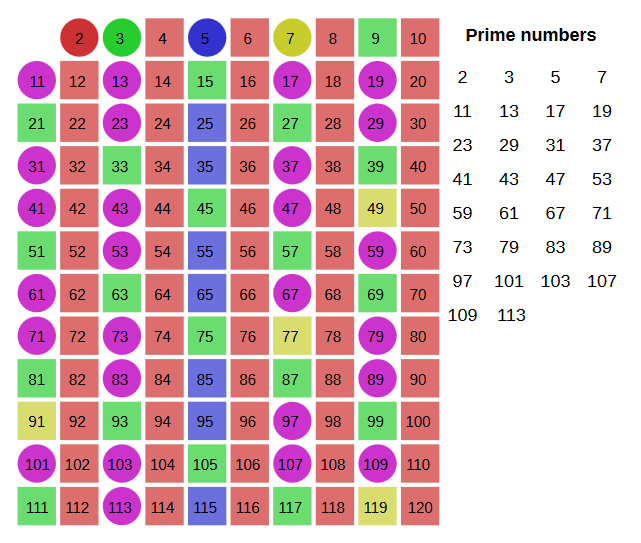
\includegraphics{figures/Primes-via-Eratosthenes-from-Wikipedia_en.png}
 }
% footnotemark, damit Nummer direkt hinter dem Titel; protect davor, um Compilierungsfehler
% zu vermeiden (http://www.undertec.de/blog/2013/06/latex-error-argument-of-caption-has-an-extra.html),
 % da es ein fragile command. footnotetext NACH end{figure}, sonst Fu�note nicht angezeigt.
 \caption[Das Sieb des Eratosthenes angewandt auf die ersten 120 Zahlen]
         {Das Sieb des Eratosthenes angewandt auf die ersten 120 Zahlen\protect\footnotemark}
\label{SieveEratosthenes01-figure}
\end{center}
\end{figure}
\footnotetext{%
   Graphik von 
   \url{https://upload.wikimedia.org/wikipedia/commons/0/0b/Sieve_of_Eratosthenes_animation.svg}
   }

Durchzuf�hren braucht man das nur bis zu der gr��ten Zahl,
deren Quadrat kleiner oder gleich $x$ ist (hier also bis 10, da $11^2$ schon $> 120$).%
\footnote{%
\index{ZT, Lernprogramm Zahlentheorie}%
\index{Lernprogramm ZT}%
Mit dem Lernprogramm {\bf ZT} k�nnen Sie f�r beliebige eigene Wertemengen
das Sieb des Eratosthenes rechnergest�tzt und gef�hrt Schritt f�r
Schritt anwenden: Siehe ZT-Lern-Kapitel 1.2, Seite 6/21 und 7/21.\\
ZT k�nnen Sie in CT1\index{CrypTool 1} �ber das Men�
{\bf Einzelverfahren \textbackslash{} Zahlentheorie interaktiv \textbackslash{}
Lernprogramm f�r Zahlentheorie} aufrufen.
    Siehe Anhang \ref{s:appendix-Learn-NT}.\\
    Eine Visualisierung dieses Verfahrens ist in CT2\index{CrypTool 2}
    in dem Tutorial \textbf{\glqq World of Primes\grqq}~enthalten.
}


Abgesehen von 2 sind Primzahlen nie gerade. Abgesehen von 2 und 5 haben Primzahlen nie die
Endziffern 2, 5 oder 0. Also braucht man sowieso nur Zahlen mit den Endziffern 1, 3, 7, 9 zu
betrachten (es gibt unendlich viele Primzahlen mit jeder dieser letzten Ziffern; vergleiche 
\cite[Bd. 1, S. 137]{pr:Tietze1973}).

Inzwischen findet man im Internet gro�e Datenbanken, die entweder viele 
Primzahlen oder die Zerlegung vieler zusammengesetzter Zahlen
in ihre Primfaktoren enthalten.


\paragraph*{Weitere interessante Themen rund um Primzahlen} \mbox{}\\
In diesem Kapitel \ref{Label_Kapitel_Primes} wurden weitere, eher zahlentheoretische 
Themen wie Teilbarkeitsregeln, Modulo-Rechnung, modulare Inverse, modulare Potenzen
und Wurzeln, chinesischer Restesatz, Eulersche Phi-Funktion und perfekte Zahlen
nicht betrachtet. Auf einige dieser Themen geht das \hyperlink{Chapter_ElementaryNT}
{{\bf n�chste Kapitel}} (Kapitel \ref{Chapter_ElementaryNT}) ein.



% --------------------------------------------------------------------------
\pagebreak
\hypertarget{h_Notes-about-primes}{}
\section{Anmerkungen zu Primzahlen}
\label{l_Notes-about-primes}

Die folgenden Anmerkungen listen einzelne interessante S�tze, Vermutungen und 
Fragestellungen zu Primzahlen auf, aber auch Kurioses und �bersichten.


% --------------------------------------------------------------------------
\vskip +20 pt
\subsection{Bewiesene Aussagen / S�tze zu Primzahlen}
\begin{itemize}

  \item Zu jeder Zahl $n$ aus ${\bf N}$ gibt es $n$ aufeinanderfolgende 
     nat�rliche Zahlen, die keine Prim"-zahlen sind.
     Ein Beweis findet sich in \cite[S. 79]{pr:Padberg1996}.


  \item Paul Erd�s\footnote{%
        Paul Erd�s\index{Erd�s, Paul}, ungarischer Mathematiker,
        26.03.1913$-$20.09.1996. }
     bewies:
     Zwischen jeder beliebigen Zahl ungleich $1$ und ihrem Doppelten gibt
     es mindestens eine Primzahl. Er bewies das Theorem nicht als erster,
     aber auf einfachere Weise als andere vor ihm.

      
  \item % \hypertarget{link-Primzahlfunktion-base-a-Proof}{}
        \label{link-Primzahlfunktion-base-a-Proof}
     Es existiert eine reelle Zahl a, so dass die Funktion
     $f: {\bf N} \rightarrow {\mathbb Z}$ mit $n \mapsto \lfloor a^{3^n}\rfloor$
     f�r alle $n$ nur Primzahlenwerte annimmt\footnote{%
     Die Gaussklammer \index{Gaussklammer} $\lfloor x \rfloor $ der
     reellwertigen Zahl $x$ ist definiert als: $\lfloor x \rfloor $ ist die
     gr��te ganze Zahl kleiner oder gleich $x$.
     } (siehe \cite[S. 82]{pr:Padberg1996}).
     Leider macht die Bestimmung von $a$ Probleme (siehe Kapitel
     \ref{link-Primzahlfunktion-base-a-Offen}).\footnote{%
     Wenn jemand wei�, wie man das beweist, w�rden wir uns sehr freuen, dies
     zu erfahren. Friedhelm Padberg sagte auf Nachfrage, er habe den
     Beweis nicht mehr.}

% \label{zahlentyp_mersenne}
% \hypertarget{GIMPS-project}{}
% \hyperlink{GIMPS-project}{GIMPS-Projekt} (Kapitel~\ref{zahlentyp_mersenne}), 


  \vskip +6 pt      
  \item \hypertarget{link-Arithmetic-sequence-of-primes}{}
     Es gibt arithmetische Primzahlfolgen \index{Primzahlfolge!arithmetische}
     beliebig gro�er L�nge.\footnote{%
     Quellen: \\
     - \url{http://users.cybercity.dk/~dsl522332/math/aprecords.htm}
         ~~~Original-Quelle\\
     - \url{http://primes.utm.edu/glossary/page.php?sort=ArithmeticSequence}
         ~~~Original-Quelle\\
     - \url{http://en.wikipedia.org/wiki/Primes_in_arithmetic_progression}\\
     - \url{http://en.wikipedia.org/wiki/Problems_involving_arithmetic_progressions}\\
     - \url{http://en.wikipedia.org/wiki/Cunningham_chain}\\
     - GEO 10 / 2004: \glqq Experiment mit Folgen\grqq\\
     - \url{http://www.faz.net}
       \glqq Hardys Vermutung -- Primzahlen ohne Ende\grqq~von Heinrich Hemme (06. Juli 2004)
     }$^,$\footnote{%  Doppelfussnote
     Arithmetische Folgen mit k Primzahlen werden auch Prime arithmetic progressions
     genannt und daher PAP-k bzw. AP-k abgek�rzt.
     }

     Die 1923 von dem ber�hmten englischen Mathematiker Hardy\footnote{%
     Godfrey Harold Hardy\index{Hardy, Godfrey Harold}, britischer
     Mathematiker, 7.2.1877$-$1.12.1947.}
     aufge"-stellte Vermutung, dass es arithmetische Folgen beliebiger L�nge
     gibt, die nur aus Prim"-zahlen bestehen, wurde 2004 von zwei jungen
     amerikanischen Mathematikern bewiesen.
  
     Jedes Schulkind lernt im Mathematikunterricht irgendwann einmal die 
     arithmetischen Zahlenfolgen kennen. Das sind Aneinanderreihungen von
     Zahlen, bei denen die Abst�nde zwischen je zwei aufeinander folgenden
     Gliedern gleich sind - etwa bei der Folge 5, 8, 11, 14, 17, 20. Der
     Abstand der Glieder betr�gt hierbei jeweils 3 und die Folge hat 6
     Folgenglieder. Eine arithmetische Folge muss mindestens 3 Folgenglieder
     haben, kann aber auch unendlich viele haben.

     Arithmetische Folgen sind seit Jahrtausenden bekannt und bergen eigentlich 
     keine Ge"-heim"-nisse mehr.
     Spannend wird es erst wieder, wenn die Glieder einer arithmetischen Folge
     noch zus�tzliche Eigenschaften haben sollen, wie das bei Primzahlen der
     Fall ist. 

     Primzahlen sind ganze Zahlen, die gr��er als 1 und nur durch 1 und sich
     selbst ohne Rest teilbar sind. Die zehn kleinsten Primzahlen sind
     2, 3, 5, 7, 11, 13,  17, 19, 23 und 29. 

     Eine arithmetische Primzahlfolge mit f�nf Gliedern ist beispielsweise 
     5, 17, 29, 41, 53. Der Abstand der Zahlen betr�gt jeweils 12. 

     Diese Folge l�sst sich nicht verl�ngern, ohne ihre Eigenschaft
     einzub��en, denn das n�chste Glied m�sste 65 sein, und diese Zahl ist
     das Produkt aus 5 und 13 und somit keine Primzahl.

     Wie viele Glieder kann eine arithmetische Primzahlfolge haben? Mit dieser
     Frage haben sich schon um 1770 der Franzose Joseph-Louis Lagrange und der
     Engl�nder Edward Waring besch�ftigt. Im Jahre 1923 vermuteten der
     ber�hmte britische Mathematiker Godfrey Harold Hardy und sein Kollege
     John Littlewood, dass es keine Obergrenze f�r die Zahl der Glieder gebe.
     Doch es gelang ihnen nicht, das zu beweisen. Im Jahr 1939 gab es jedoch
     einen anderen Fortschritt: Der holl�ndische Mathematiker Johannes van der
     Corput konnte nachweisen, dass es unendlich viele arithmetische
     Primzahlfolgen mit genau drei Gliedern gibt. Zwei Beispiele hierf�r sind
     3, 5, 7  und  47, 53, 59.

     Die l�ngste Primzahlfolge, die man bisher kennt, hat 25 Glieder.
     In der Tabelle~\ref{Smallest AP-k with minimal difference}
     sind die l�ngsten bekannten arithmetischen
     Primzahlfolgen mit minimaler Distanz\footnote{%
        Dagegen sind in
        \url{http://en.wikipedia.org/wiki/Primes_in_arithmetic_progression}
        die \glqq Largest known AP-k\grqq~aufgelistet.
        Also ist dort das letzte Folgenelement eine m�glichst gro�e Primzahl.\\
        Tabelle \ref{Smallest AP-k with minimal difference} listet jedoch die Folgen auf, die die kleinsten bekannten
        Differenzen haben -- f�r eine gegebene Folgenl�nge.
     }
     aufgelistet.

     Den beiden jungen\footnote{%
     In seinen Memoiren hat Hardy\index{Hardy, Godfrey Harold} 1940 geschrieben, 
     dass die Mathematik mehr als alle anderen Wissenschaften und K�nste 
     ein Spiel f�r junge Leute sei. \\
     Der damals 27 Jahre alte Ben Green von der University of British Columbia
     in Vancouver und der damals 29 Jahre alte Terence Tao\index{Tao, Terence} von der
     University of California in Los Angeles scheinen ihm recht zu geben.
     }
     Mathematikern  Ben Green and Terence Tao ist es im Jahre 2004 gelungen,
     die mehr als achtzig Jahre alte Hardysche Vermutung zu beweisen: 
     Es gibt arithmetische Primzahlfolgen beliebiger L�nge. Au�erdem bewiesen
     sie, dass es zu jeder vorgegebenen L�nge unendlich viele verschiedene
     solcher Folgen gibt.

     Eigentlich hatten Green und Tao nur beweisen wollen, dass es unendlich
     viele arithmetische Primzahlfolgen mit vier Gliedern gibt. Dazu
     betrachteten sie Mengen, die neben Primzahlen auch 
     Beinaheprimzahlen\index{Beinaheprimzahl}\index{Primzahl!Beinaheprimzahl} 
     enthielten. Das sind Zahlen, die nur wenige Teiler haben - beispielsweise
     die Halbprimzahlen%
     \index{Halbprimzahl}\index{Primzahl!Halbprimzahl}%
     \index{Zahlen!semiprime}\index{Zahlen!Halbprimzahl},
     die Produkte aus genau zwei Primzahlen sind.
     Dadurch konnten die beiden Mathematiker ihre Arbeit wesentlich
     erleichtern, denn �ber Beinaheprimzahlen gab es schon zahlreiche
     n�tzliche Theoreme. Schlie�lich erkannten sie, dass ihr Verfahren viel
     m�chtiger ist, als sie selbst angenommen hatten, und sie bewiesen damit
     die Hardysche Vermutung.
 
     Der Beweis von Green und Tao umfasst immerhin 49 Seiten. Tats�chlich
     beliebig lange arithmetische Primzahlfolgen kann man damit aber nicht
     finden. Der Beweis ist nicht konstruktiv, sondern ein so genannter 
     Existenzbeweis\index{Beweis!Existenzbeweis}\index{Beweis!konstruktiv}. 
     Das hei�t, die beiden Mathematiker haben \glqq nur\grqq~gezeigt, dass 
     beliebig lange Folgen existieren, aber nicht, wie man sie findet.

     Das hei�t, in der Menge der nat�rlichen Primzahlen gibt es zum Beispiel
     eine Folge von einer Milliarde Primzahlen, die alle den gleichen Abstand 
     haben; und davon gibt es unendlich viele. Diese Folgen liegen aber sehr 
     \glqq weit drau�en\grqq.   %\glqq D\grqq~


     \begin{table}[ht]
     \begin{center}
     \begin{tabular}{|r|r|r|r|r|}
     \hline
     Elemente & Startelement & Abstand & Wann   & Entdecker \\
              &              &         & Digits &           \\ \hline

      3 &                   3 &                   2 &      & \\
        &                     &                     &    1 & \\
	&&&& \\
 
      4 &                   5 &                   6 &      & \\
        &                     &                     &    2 & \\
	&&&& \\

      5 &                   5 &                   6 &      & \\
        &                     &                     &    2 & \\
	&&&& \\
 
      6 &                   7 &                  30 & 1909 & G. Lenaire \\
        &                     &                     &    3 & \\
	&&&& \\
 
      7 &                   7 &                 150 & 1909 & G. Lenaire \\
        &                     &                     &    3 & \\
  
....... &                     &                     &      & \\
	&&&& \\

     21 & 28.112.131.522.731.197.609 &          9.699.690 & 2008 & Jaroslaw Wroblewski\\
        &                            &              $= 19\#$ &   20 & \\
	&&&& \\
 
     22 &        166.537.312.120.867 &     96.599.212.710 & 2006 & Markus Frind\\
        &                            &        = 9.959�19\# &   15 & \\
	&&&& \\

     23 &        403.185.216.600.637 &  2.124.513.401.010 & 2006 & Markus Frind,\\
        &                            &        = 9.523�23\# &   15 & \\
	&&&& \\

     24 &        515.486.946.529.943 & 30.526.020.494.970 & 2008 & Raanan Chermoni,\\
        &                            &      = 136.831�23\# &   16 & Jaroslaw Wroblewski\\
	&&&& \\
 
     25 &      6.171.054.912.832.631 & 81.737.658.082.080 & 2008 & Raanan Chermoni,\\
        &                            &      = 366.384�23\# &   16 & Jaroslaw Wroblewski\\
  
     \hline
     \end{tabular}
     \caption{Arithmetische Primzahlfolgen mit minimaler Distanz (Stand Aug. 2012)}
     \label{Smallest AP-k with minimal difference}
     \end{center}
     \end{table}
     \clearpage

     Wer solche Folgen entdecken m�chte, sollte folgendes ber�cksichtigen.
     Die L�nge der Folge bestimmt den Mindestabstand zwischen den einzelnen
     Primzahlen. Bei einer Folge mit $k=6$ Gliedern muss der Abstand 30 oder ein
     Vielfaches davon betragen. Die Zahl 30 ergibt sich als das Produkt aller
     Primzahlen, die kleiner als die Folgenl�nge, also kleiner als 6, sind:
     $ 6\# = 5\# = 2 * 3 * 5 = 30 $.
     Noch ein Beispiel: $ 10\# = 7\# = 2 * 3 * 5 * 7 = 210$.
     Sucht man Folgen mit der L�nge 15, so muss der 
     Abstand mindestens $ 15\# = 13\# = 2 * 3 * 5 * 7 * 11 * 13 = 30.030 $ betragen.
     \index{Primzahl!k Primorial} \index{Primzahl!k\#}   

     Daraus ergibt sich, dass die Folgenl�nge beliebig gro� sein kann, aber
     der Abstand kann nicht nicht jede beliebige Zahl annehmen: es kann keine
     arithmetische Primzahlfolge mit dem Abstand $100$ geben, denn 100 ist
     nicht durch die Zahl 3 teilbar.

     \begin{table}[ht]
     \begin{center}
     \hspace*{1cm}\begin{tabular}{|r|r|}
     \hline
      k &                k\# \\ \hline
      2 &                 2 \\
      3 &                 6 \\
      5 &                30 \\
      7 &               210 \\
     11 &             2.310 \\
     13 &            30.030 \\
     17 &           510.510 \\
     19 &         9.699.690 \\
     23 &       223.092.870 \\
      \hline
     \end{tabular}
     \caption{Produkte der ersten Primzahlen $<= k$ (genannt k Primorial oder $k\#$)}
     \end{center}
     \end{table}


     \vskip +10 pt
     {\bf Weitere Restriktion an die arithmetische Folge:}\\
     Sucht man arithmetische Primzahlfolgen, 
     die die {\em zus�tzliche} Bedingung erf�llen, dass alle Primzahlen
     in der Folge auch {\em direkt hintereinander} liegen (consecutive
     primes sequence\footnote{%
     Sie werden auch consecutive prime arithmetic progressions genannt
     und daher CPAP-k bzw. CAP-k abgek�rzt.
     }), wird es noch etwas schwieriger. Auf der 
     Webseite von Chris Caldwell\footnote{%
     \url{http://primes.utm.edu/glossary/page.php?sort=ArithmeticSequence}
     } 
     finden Sie weitere Informationen: Die l�ngste bekannte arithmetische
     Folge, die nur aus direkt hintereinander liegenden Primzahlen besteht
     (Stand Aug. 2012), hat die L�nge $10$, der Abstand betr�gt
     $$ 10\# = 7\# = 2 * 3 * 5 * 7 = 210 $$
     und sie startet mit der 93-stelligen Primzahl\\
     100 9969724697 1424763778 6655587969 8403295093 2468919004 1803603417 7589043417 0334888215 9067229719\\


\end{itemize}



% --------------------------------------------------------------------------
% \vskip +10 pt
\newpage
\subsection{Verschiedene unbewiesene Aussagen / Vermutungen / offene Fragestellungen zu Primzahlen}
\begin{itemize}
  \item Goldbach\footnote{%
     Christian Goldbach\index{Goldbach, Christian}, deutscher Mathematiker,
     18.03.1690$-$20.11.1764. }
     vermutete:
     Jede gerade nat�r"-liche Zahl gr��er $2$ l�sst sich als die Summe
     zweier Primzahlen darstellen.\footnote{Vergleiche auch Kapitel
     \ref{L-GoldbachConjecture}.}


\item Riemann\footnote{%
        Bernhard Riemann\index{Riemann, Bernhard}, deutscher Mathematiker,
        17.9.1826$-$20.7.1866. }
     stellte eine wichtige, bisher unbewiesene Hypothese\footnote{%
        \url{http://de.wikipedia.org/wiki/Riemannsche_Vermutung}  }
     �ber die Nullstellen der Riemannschen Zetafunktion auf, aus der auch eine
     verbesserte Restglied"-ab"-sch�t"-zung im Primzahlsatz (Verteilung von
     Primzahlen) folgt.


\item Das Benfordsche Gesetz\label{primes:Benford-Law}\footnote{%
        \url{http://de.wikipedia.org/wiki/Benfordsches_Gesetz}, \\
        \url{http://www.spiegel.de/wissenschaft/mensch/0,1518,632541,00.html},\\
        \url{http://arxiv.org/PS_cache/arxiv/pdf/0906/0906.2789v1.pdf}. 
        }$^,$\footnote{%
        Didaktische Darstellungen zu Anwendungen von Benfords Gesetz finden sich
        unter:
        % \begin{itemize}
        \begin{compactitem}
         \item R�deger Baumann: \glqq Ziffernanalyse zwecks Betrugsaufdeckung
              --- Beispiel f�r kompetenzorientierten und kontextbezogenen
              Informatikunterricht\grqq, \\
              in LOGIN, Informatische Bildung und Computer in der Schule,
              Nr. 154/155, 2008, S. 68-72
         \item Norbert Hungerb�hler: \glqq Benfords Gesetz �ber f�hrende
              Ziffern\grqq, \\
              M�rz 2007,
              \url{http://www.educ.ethz.ch/unt/um/mathe/ana/benford}
        \end{compactitem}
        % \end{itemize}
        %\vspace{-\baselineskip} % TODO: Geht das nicht anders? N�tzte nichts.
        \vspace{-\baselineskip} % N�tzte nichts.
        }
     gilt nicht f�r Primzahlen. 

     Nach dem Benfordschen Gesetz sind die Ziffern
     in den Zahlen bestimmter empirischer Datens�tze (z.B. �ber Einwohnerzahlen
     von St�dten, Geldbetr�ge in der Buchhaltung, Naturkonstanten) ungleichm��ig
     verteilt: Z.B. ist die Ziffer \verb#1# viel h�ufiger die erste Ziffer
     einer Zahl als jede andere.

     Welche Datens�tze diesem Gesetz gehorchen ist noch nicht vollst�ndig
     gekl�rt. Timo Eckhardt untersuchte in seiner Diplomarbeit 2008 ausf�hrlich
     Eigenschaften von Primzahlen. Unter anderem wurden alle Primzahlen bis
     7.052.046.499 mit verschiedenen Stellenwert-Basen dargestellt.
    
     Beim Vergleich der Basen 3 bis 10 ergab sich, dass die Abweichung von
     Benfords Gesetz bei der Basis 3 am geringsten ist. F�r die Basis zehn
     besteht in etwa eine Gleichverteilung der ersten Ziffern. Bei der
     Untersuchung gr��erer Basen ergab sich, dass die Verteilung der ersten
     Ziffern von Basis zu Basis sehr starke Unterschiede aufweist.



\item % \hypertarget{link-Primzahlfunktion-base-a-Offen}{}
      \label{link-Primzahlfunktion-base-a-Offen}
    Der in Kapitel \ref{link-Primzahlfunktion-base-a-Proof} erw�hnte Beweis zu
    der Funktion  $f: \: N \rightarrow Z$ mit $n \mapsto \lfloor a^{3^n}\rfloor$
    garantiert nur die Existenz einer
    solchen Zahl $a$.  Wie kann diese Zahl $a$ bestimmt werden, und wird sie
    einen Wert haben, so dass die Funktion auch von praktischem Interesse ist?


\item Gibt es unendlich viele Mersenne-Primzahlen?
   \index{Primzahl!Mersenne}\index{Mersenne!Mersenne-Primzahl}

\item Gibt es unendlich viele Fermatsche Primzahlen?


\item Gibt es einen Polynomialzeit-Algorithmus\index{Polynom} zur 
   Zerlegung einer Zahl in ihre Primfaktoren (vgl. \cite[S. 167]{pr:Klee1997})?
   Diese Frage kann man auf die folgenden drei Fragestellungen aufsplitten:
   \begin{itemize}
        \item Gibt es einen Polynomialzeit-Algorithmus, der entscheidet, ob 
	   eine Zahl prim ist? \\
	   Diese Frage wurde durch den AKS-Algorithmus\index{AKS} 
	   beantwortet (vgl.  Kapitel \ref{PrimesinP}, \glqq PRIMES in P\grqq:
	   Testen auf Primalit�t ist polynominal).
        \item Gibt es einen Polynomialzeit-Algorithmus, mit dem man 
           feststellen kann, aus wievielen Primfaktoren eine zusammengesetzte
           Zahl besteht (ohne diese Primfaktoren zu berechnen)?
        \item Gibt es einen Polynomialzeit-Algorithmus, mit dem sich f�r 
	   eine zusammengesetzte Zahl $n$ ein nicht-trivialer (d.h. 
	   von $1$ und von $n$ verschiedener) Teiler von $n$ berechnen 
	   l�sst?\footnote{Vergleiche auch Kapitel \ref{RSABernstein} 
	   und Kapitel \ref{nt:NoteFactorization}.}
   \end{itemize}

   Am Ende von Kapitel \ref{nt:NoteFactorization}, 
   Abschnitt \hyperlink{RSA-200-chap3}{RSA-200}
   k�nnen Sie die Gr��enordnungen ersehen, f�r die heutige Algorithmen
   bei Primzahltests\index{Primzahltest} und bei der
   Faktorisierung\index{Faktorisierung!Faktorisierungsrekorde} gute
   Ergebnisse liefern.

\end{itemize}



% --------------------------------------------------------------------------
\vskip +10 pt
\hypertarget{HT-GoldbachConjecture}{}
\subsection{Die Goldbach-Vermutung}
\label{L-GoldbachConjecture}

Hier soll noch etwas tiefer auf auf die
\textbf{Goldbach-Vermutung}\index{Goldbach-Vermutung}\footnote{%
        \url{http://de.wikipedia.org/wiki/Goldbachsche_Vermutung} }
eingegangen werden.



%\vskip +25 pt
\hypertarget{HT-WeakGoldbachConjecture}{}
%\paragraph*{Die schwache Goldbach-Vermutung\footnote{%
%   Sie wird auch \textbf{ungerade} oder \textbf{tern�re} Goldbach-Vermutung
%   genannt.
%   } }%
%\subsubsubsection{xxx} 3*sub kennt er nicht, deshalb vorher paragraph !
% Ohne [] vor der { l�sst er footnote nicht zu!
\subsubsection[Die schwache Goldbach-Vermutung]%
   {Die schwache Goldbach-Vermutung\footnote{%
   Sie wird auch \textbf{ungerade} oder \textbf{tern�re} Goldbach-Vermutung
   genannt.
   } }%
\index{Goldbach-Vermutung!schwache}%
\label{L-WeakGoldbachConjecture}%
%\mbox{}

\noindent Goldbach stellte 1742 in einem Brief an den Mathematiker Euler die Behauptung auf:

Jede \textbf{ungerade} nat�rliche Zahl gr��er als 5 ist als Summe von \textbf{genau drei} Primzahlen darstellbar.

Beispiele: $7 = 3 + 2 + 2$ oder $27 = 19 + 5 + 3$ oder $27 = 17 + 5 + 5$

\noindent Diese Behauptung ist immer noch (seit �ber 250 Jahren) unbewiesen.

\noindent Mit Computern ist die \textbf{schwache Goldbach-Vermutung} f�r alle
ungeraden nat�rlichen Zahlen einfach bis $4*10^{18}$ (Stand April 2012) bzw.
doppelt bis  $4*10^{17}$ (Stand Mai 2013) verifiziert.\footnote{%
Siehe \url{http://sweet.ua.pt/tos/goldbach.html} von Tom�s Oliveira e Silva
     }

Aus fr�heren Arbeiten ist bekannt, dass die schwache Goldbach-Vermutung
f�r alle ungeraden Zahlen gr��er $e^{3100}\approx 2 \times 10^{1346}$ wahr ist.

Wie bei vielen ber�hmten Vermutungen in der Mathematik gibt es auch f�r die
Goldbach-Vermutung eine Reihe angeblicher Beweise, die aber von der
mathematischen Gemeinschaft (noch) nicht akzeptiert sind.\footnote{%
Einer davon ist in dem Paper von Shan-Guang Tan, das am 16. Okt. 2011 (v1)
ver�ffentlicht, und zuletzt am 26. Juni 2013 (v11) revidiert wurde. Es
behauptet, sogar die starke Goldbach-Vermutung zu beweisen.\\
v1 hat den Titel \glqq A proof of the Goldbach conjecture\grqq.\\
v11 hat den Titel \glqq On the representation of even numbers as the sum and difference of two primes and the representation of odd numbers as the sum of an odd prime and an even semiprime and the distribution of primes in short intervals\grqq.\\
Siehe \url{http://arxiv.org/abs/1110.3465}.
   }

Eine Vorarbeit f�r einen Beweis k�nnte die k�rzlich\footnote{\url{http://arxiv.org/abs/1201.6656}, eingereicht am 31. Jan. 2012 (v1), letzte �nderung 3. Juli 2012 (v4)} vorgestellte Arbeit von Terence Tao\index{Tao, Terence} von der University of California sein. Er bewies, dass sich jede \textbf{ungerade} nat�rliche Zahl gr��er 1 als Summe von \textbf{h�chstens f�nf} Primzahlen darstellen l�sst.

Inzwischen gab es erhebliche Arbeiten an der schwachen Goldbach-Vermutung. Sie
kulminierten 2013 in der Behauptung von Harald Helfgott, die Vermutung komplett
f�r alle nat�rlichen Zahlen gr��er 7 bewiesen zu haben.\footnote{%
Helfgott, H.A. (2013): \glqq Major arcs for Goldbach's theorem\grqq.
\url{http://arxiv.org/abs/1305.2897}.\\
v2 seines 133-seitigen Papers (14. Juni 2013) besagt, dass der Beweis f�r alle
nat�rlichen Zahlen ab $10^{29}$ (statt bisher $10^{30})$ gilt. Und f�r alle
Zahlen bis $10^{30}$ behauptet er, dass er und David Platt den Beweis durch
Probieren am Computer erbrachten.
\\
\url{http://truthiscool.com/prime-numbers-the-271-year-old-puzzle-resolved}.\\
\url{http://www.newscientist.com/article/dn23535-proof-that-an-infinite-number-of-primes-are-paired.html#.UgwhOpL0Ek0}.\\
\url{http://www.spiegel.de/wissenschaft/mensch/beweis-fuer-schwache-goldbachsche-vermutung-a-901111.html}.
}



%\vskip +25 pt
\hypertarget{HT-StrongGoldbachConjecture}{}
%\subsubsubsection{xxx} 3*sub kannte er nicht, deshalb paragraph !
\subsubsection[Die starke Goldbach-Vermutung]%
   {Die starke Goldbach-Vermutung\footnote{%
   Sie wird auch \textbf{gerade} oder \textbf{bin�re} Goldbach-Vermutung
   genannt.
   } }%
\index{Goldbach-Vermutung!starke}%
\label{L-StrongGoldbachConjecture}%
%\mbox{}

\noindent Goldbachs starke Primzahlhypothese wurde von Euler nach einem Briefwechsel mit Goldbach formuliert, und wird meist einfach als \textbf{die} Goldbach-Vermutung bezeichnet:

Jede \textbf{gerade} nat�rliche Zahl gr��er als 2 ist als Summe von \textbf{genau zwei} Primzahlen darstellbar.

Beispiele f�r Goldach-Zerlegungen: $8 = 5 + 3$ oder $28 = 23 + 5$

\noindent Mit Computern ist die \textbf{Goldbach-Vermutung}\index{Goldbach-Vermutung}
     f�r alle geraden Zahlen bis $4*10^{18}$ (Stand Mai 2013) einfach
     verifiziert\footnote{%
     Dass die Goldbach-Vermutung wahr ist, d.h. f�r alle geraden 
     nat�rlichen Zahlen gr��er als $2$ gilt, wird heute allgemein nicht 
     mehr angezweifelt. Der Mathematiker J�rg Richstein\index{Richstein 1999}
     vom Institut f�r Informatik der Universit�t Gie�en hat 1999 die geraden
     Zahlen bis 400 Billionen ($4*10^{14}$) untersucht (\cite{pr:Richstein1999})
     und kein Gegenbeispiel gefunden.\\
     Inzwischen wurden noch umfangreichere �berpr�ngen bis vorgenommem: Siehe\\ 
     \url{http://sweet.ua.pt/tos/goldbach.html} von Tom�s Oliveira e Silva, \\
     \url{http://www.ieeta.pt/~tos/goldbach.html} von Tom�s Oliveira e Silva, \\
     \url{http://de.wikipedia.org/wiki/Goldbachsche\_Vermutung},\\
     \url{http://primes.utm.edu/glossary/page.php/GoldbachConjecture.html}.\\
     % http://www.mscs.dal.ca/\~{}joerg/res/g-en.html
     Trotzdem ist das kein allgemeiner Beweis.\\ 
     Dass die Goldbach-Vermutung trotz aller Anstrengungen bis heute 
     nicht bewiesen wurde, l�sst Folgendes bef�rchten:
     Seit den bahnbrechenden Arbeiten des �sterreichischen Mathematikers 
     Kurt G�del\index{G�del, Kurt} ist bekannt, dass nicht jeder wahre
     Satz in der Mathematik auch beweisbar ist (siehe 
     \url{http://www.mathematik.ch/mathematiker/goedel.html}).
     M�glicherweise hat Goldbach also Recht, und trotzdem wird nie ein 
     Beweis gefunden werden. Das wiederum l�sst sich aber vermutlich auch
     nicht beweisen.
     },   % end_footnote
     aber allgemein noch nicht bewiesen.\footnote{%
     Der englische Verlag {\em Faber} und die amerikanische
     Verlagsgesellschaft {\em Bloomsbury} publizierten 2000 das 1992 erstmals
     ver�ffentlichte Buch \glqq Onkel Petros und die Goldbachsche 
     Vermutung\grqq~ von Apostolos Doxiadis (deutsch bei
     L�bbe 2000 und bei BLT als Taschenbuch 2001). Es ist 
     die Geschichte eines Mathematikprofessors, der daran scheitert, ein 
     mehr als 250 Jahre altes R�tsel zu l�sen.\\
     Um die Verkaufszahlen zu f�rdern, schrieben die beiden Verlage einen 
     Preis von 1 Million USD aus, wenn jemand die Vermutung beweist -- 
     ver�ffentlicht in einer angesehenen mathematischen Fachzeitschrift 
     bis Ende 2004.\\
     Erstaunlicherweise durften nur englische und amerikanische Mathematiker
     daran teilnehmen.
     }${}^,$\footnote{%
     Die Aussage, die der starken Goldbach-Vermutung bisher am n�chsten kommt,
     wurde 1966 von Chen Jing-Run bewiesen -- in einer schwer nachvollziehbaren
     Art und Weise: Jede gerade Zahl gr��er 2 ist die Summe einer Primzahl und
     des Produkts zweier Primzahlen. Z.B. $20=5+3*5.$\\ 
     Die wichtigsten Forschungsergebnisse zur Goldbach-Vermutung sind
     zusammengefasst in dem von Wang Yuan herausgegebenen Band: 
     \glqq Goldbach Conjecture\grqq, 1984, World Scientific Series in Pure
     Maths, Vol. 4.
     }${}^,$\footnote{%
     Gerade diese Vermutung legt nahe, dass wir auch heute noch nicht in 
     aller Tiefe den Zusammenhang zwischen der Addition und der Multiplikation
     der nat�rlichen Zahlen verstehen.
     }  % end_footnote

Je gr��er eine gerade Zahl ist, umso mehr solcher bin�rer Goldbach-Zerlegungen lassen sich im Durchschnitt finden: F�r $4$ gibt es nur eine Zerlegung $2 + 2$; bei $16$ sind es schon zwei, n�mlich $3 + 13$ und $5 + 11$. Bei $100$ sind es sechs $3 + 97$, $11 + 89$, $17 + 83$, $29 + 71$, $41 + 59$, $47 + 53$.\footnote{%
     Vergleiche \url{http://www.spiegel.de/wissenschaft/mensch/primzahlraetsel-loesung-der-goldbachschen-vermutung-rueckt-naeher-a-833216.html}. Dieser Artikel geh�rt in die Reihe der gut lesbaren Numerator-Kolumnen in Spiegel-Online von Holger Dambeck.
% Andere gute Kolumne zu seinen Forschungsergebnissen: http://terrytao.wordpress.com/
% Andere Disk.: http://mathforum.org/kb/message.jspa?messageID=7818160
% http://www.ams.org/news/math-in-the-media/06-2012-media
% http://aperiodical.com/2012/02/every-odd-integer-larger-than-1-is-the-sum-of-at-most-five-primes/
% http://oumathclub.wordpress.com/category/on-the-web/page/2/
% Vgl.: http://oumathclub.wordpress.com/  press column
     }   % end_footnote




\vskip +35 pt %Gr��er gemacht als 15, damit die ff. �berschrift nicht alle am Seitenende 
%\subsubsubsection{xxx} 3*sub kannte er nicht, deshalb paragraph !
\subsubsection{Zusammenhang zwischen den beiden Goldbach-Vermutungen}%
%\mbox{}

\noindent Wenn die starke Goldbach-Vermutung gilt, gilt auch die schwache (d.h. die starke impliziert die schwache Vermutung).

Der Beweis daf�r ist relativ einfach:\\
Voraussetzung: Sei $u$ eine ungerade Zahl gr��er als $5$.\\
Jede solche ungerade Zahl $u$ kann als Summe
$u = (u-3) + 3$ geschrieben werden. Der erste Summand ist dann gerade und $>= 4$, erf�llt
damit die Voraussetzung der starken Goldbach-Vermutung und kann damit als Summe zweier
Primzahlen $p_1$ und $p_2$ geschrieben werden (wobei $p_1$ und $p_2$ nicht notwendigerweise verschieden sein m�ssen). Damit hat man eine Zerlegung von $u$ in die drei Primzahlen $p_1, p_2$ und $3$ gefunden.
D.h. man kann sogar immer eine Summe finden, in der einer der drei primen Summanden die Zahl $3$ ist.

�hnlich einfach kann man zeigen, dass aus der schwachen Golfbach-Vermutung die
oben erw�hnte Behauptung von Terence Tao folgt (beide gelten f�r ungerade
Zahlen):
\begin{itemize}	
   \item F�r ungerade Zahlen $u>5$ folgt direkt aus der schwachen
      Goldbach-Vermutung, dass die Summe aus h�chstens f�nf Primzahlen besteht.
   \item F�r die restlichen ungeraden Zahlen $3$ und $5$ kann man es direkt
      einsetzen:\\
      $3 = 3$ (die \glqq Summe\grqq~hat nur einen und damit h�chstens
      f�nf prime Summanden);\\
      $5 = 2 + 3$ (die Summe hat zwei und damit h�chstens f�nf prime Summanden).
\end{itemize}




% --------------------------------------------------------------------------
\vskip +35 pt
\hypertarget{HT-TwinCousinPrimes}{}
\subsection{Offene Fragen zu Primzahlzwillingen und Primzahl-Cousins}
\label{L-TwinCousinPrimes}

Primzahlzwillinge\index{Primzahlzwilling} sind Primzahlen, die genau den
Abstand 2 voneinander haben, zum Beispiel 5 und 7, oder 101 und 103,
oder $1.693.965 \cdot 2^{66.443} \pm 1$. 

\noindent Das gr��te heutzutage bekannte Primzahlzwillingspaar
\[3.756.801.695.685\cdot 2^{666.669} \pm 1\] wurde im
Dezember 2011 gefunden und hat $200.700$ Dezimalstellen.\footnote{%
   \url{http://primes.utm.edu/primes},
   \url{http://www.primegrid.com/download/twin-666669.pdf}}


\noindent Offen ist:
\begin{itemize}
\item Gibt es unendlich viele oder eine begrenzte Anzahl von
      Primzahlzwillingen?\footnote{%
      Bemerkung: Primzahl-{\bf Drillinge} gibt es dagegen nur eines: 3, 5, 7.
      Bei allen anderen Dreierpacks aufeinanderfolgender ungerader Zahlen ist
      immer eine durch 3 teilbar und somit keine Primzahl.
                                  }${}^,$\footnote{%
      Die Vermutung, dass es unendlich viele Primzahlzwillinge gibt, ist nicht
      selbstverst�ndlich. Man wei�, dass bei gro�en Zahlen im Durchschnitt der
      Abstand zwischen Primzahlen immer weiter w�chst und ca. 2,3 mal so gro�
      ist wie die Anzahl der Dezimalstellen. Beispielsweise betr�gt bei 
      100-stelligen Dezimalzahlen der Abstand zwischen Primzahlen im
      Durchschnitt 230.
      Aber diese Aussage gilt nur f�r den Durchschnitt -- oft ist der Abstand
      viel gr��er, oft viel kleiner.
                                  }${}^,$\footnote{%
      \url{http://de.wikipedia.org/wiki/Primzahlzwilling}
      }

\item Gibt es eine Formel f�r die Anzahl der Primzahlzwillinge pro Intervall?
\end{itemize}

\noindent Im Folgenden werden zwei gr��ere Meilensteine erl�utert, die dem
R�tsel n�her kommen.


\subsubsection{GPY 2003}

Einen gro�en Schritt zur Kl�rung der ersten Frage machten m�glicherweise
Dan Goldston, J\'{a}nos Pintz und Cem Yildirim im Jahre 2003.\footnote{%
    D. A. Goldston: \glqq Gaps Between Primes\grqq \\
    \url{http://www.math.sjsu.edu/~goldston/OberwolfachAbstract.pdf}\\ 
    Siehe auch: 
    \begin{compactitem}
       \item D. A. Goldstone: \glqq Are There Infinitely Many Twin Primes?\grqq, \\
            \url{http://www.math.sjsu.edu/~goldston/twinprimes.pdf}
       \item K. Soundararajan: \glqq Small Gaps Between Prime Numbers:
             The Work Of Goldston-Pintz-Yildirim\grqq, \\
             \url{http://www.ams.org/bull/2007-44-01/S0273-0979-06-01142-6/S0273-0979-06-01142-6.pdf}
    \end{compactitem}
    \vspace{-\baselineskip} % TODO: Geht das nicht anders?
                                              }
Die drei Mathematiker besch�ftigten sich mit der Verteilung von Primzahlen.
Sie konnten beweisen, dass  \[ \liminf_{n\to\infty}{\frac{p_{n+1}-p_n}{\log{p_n}}}=0,\]
wobei $p_{n}$ die $n$-te Primzahl bezeichnet. \\
Dies bedeutet, dass der kleinste H�ufungspunkt ($\liminf$) der Folge
$\frac{p_{n+1}-p_n}{\log{p_n}}$ gleich Null ist.\\
Ein Punkt hei�t H�ufungspunkt einer Folge, wenn in jeder noch so kleinen
Umgebung um diesen Punkt unendlich viele Folgeglieder liegen. \\
$\log{p_n}$ ist in etwa der erwartete Abstand zwischen der Primzahl $p_n$
und der darauf folgenden Primzahl $p_{n+1}$.\\
Der obige Term besagt also, dass es unendlich viele aufeinander folgende
Primzahlen gibt, deren Abstand im Verh�ltnis zum erwarteten durchschnittlichen
Abstand beliebig nah an Null bzw. beliebig klein ist.

Au�erdem konnte gezeigt werden, dass f�r unendlich viele Primzahlen
gilt\footnote{ c't 2003, Heft 8, Seite 54}: \[p_{n+1}-p_n < (\log{p_n})^{8/9}\]



\subsubsection{Zhang 2013}

Im Mai 2013 wurde die Arbeit von Yitang Zhang\index{Zhang, Yitang}
bekannt.\footnote{%
   Erica Klarreich (19. Mai 2013): \glqq Unheralded Mathematician Bridges the
   Prime Gap\grqq \\
   \url{https://www.simonsfoundation.org/quanta/20130519-unheralded-mathematician-bridges-the-prime-gap/}}
Zhang beweist, dass es unendlich viele \glqq Primzahl-Cousins\grqq~gibt, oder
genauer, dass es unendlich viele Primzahlpaare gibt, die einen Abstand von $H$
haben und dass die Zahl $H$ kleiner als 70 Millionen ist.\footnote{%
W�hrend bei einem Primzahl-Zwilling der Abstand der beiden Primzahlen genau
$2$ ist, bezeichnen Primzahl-Cousins\index{Primzahl-Cousin} zwei Primzahlen,
deren Abstand den Wert einer gr��eren geraden, aber endlichen Zahl $H$ hat.
      }${}^,$\footnote{%
Dies ist nahezu der Beweis f�r die Vermutung, die 1849 von dem franz�sichen
Mathematiker Alphonse de Polignac aufgestellt wurde, dass es unendlich viele
Primzahl-Paare gibt zu jeder m�glichen geraden und endlichen L�cke (nicht nur
f�r die $2$).
       }${}^,$\footnote{%
In weiteren Arbeiten wurde dieser Mindestabstand $H$ gleich 70 Millionen
inzwischen weiter verbessert. Diese Fortschritte werden im 8. Polymath-Projekt
(massively collaborative online mathematical projects)) dokumentiert: "Bounded
gaps between primes". Der beste bisher bekannte Werte f�r $H$ (Stand August
2013) ist $4680$ -- das ist ein guter Fortschritt gegen�ber 70 Millionen, aber
immer noch weit entfernt von $2$.\\
Siehe \url{http://michaelnielsen.org/polymath1/index.php?title=Bounded_gaps_between_primes}
       }

Diese Aussagen k�nnten Grundlage sein um zu beweisen, dass es unendlich
viele Primzahl"-zwillinge gibt.



% --------------------------------------------------------------------------
%\vskip +25 pt
\newpage
% Die eckigen Klammern sind n�tig, will man \footnotmark innerhalb der {}
% verwenden.
% Man muss den Titel sowohl in die [] als auch in die {} stellen:
% - Fehlt er innerhalb {}, ist die �berschrift innerhalb des Textes leer.
% - Fehlt er innerhalb [], fehlt die �berschrift links im PDF-Rahmen und
%   im Inhaltsverzeichnis.
\subsection[Kurioses und Interessantes zu Primzahlen]
              {Kurioses und Interessantes zu Primzahlen\footnotemark}
    \footnotetext{%
Weitere kuriose und seltsame Dinge zu Primzahlen finden sich auch unter:\\
- \url{http://primes.utm.edu/curios/home.php}\\
- \url{http://www.primzahlen.de/files/theorie/index.htm}.
}
\label{HT-Quaint-curious-Primes-usage}

Primzahlen sind nicht nur ein sehr aktives und ernstes mathematisches
Forschungsgebiet. Mit ihnen besch�ftigen sich Menschen auch hobbym��ig und
au�erhalb der wissenschaftlichen For"-schung.


\vskip +25 pt
\hypertarget{HT-GoogleRecruitment2004}{}
\subsubsection{Mitarbeiterwerbung bei Google im Jahre 2004}
% \paragraph*{Mitarbeiterwerbung bei Google im Jahre 2004}%
\index{Google!Mitarbeiterwerbung}%
\label{HT-GoogleRecruitment2004}%
\mbox{}
Im Sommer 2004 benutzte die Firma Google die Zahl $e$, um Bewerber zu
gewinnen.\footnote{Die Basis des nat�rlichen Logarithmus\index{Logarithmus!nat�rlicher}
$e$ ist ungef�hr 2,718 281 828 459.
Dies ist eine der bedeutendsten Zahlen in der Mathematik. Sie wird gebraucht
f�r komplexe Analysis, Finanzmathematik, Physik und Geometrie. Nun wurde sie
-- meines Wissens -- das erste Mal f�r Marketing oder Personalbeschaffung
verwendet.}${}^,$\footnote{Die meisten Informationen f�r diesen Paragraphen
stammen aus dem Artikel \glqq e-number crunching\grqq~ von John Allen Paulos
in TheGuardian vom 30.09.2004 und aus dem Internet:\\
- \url{http://www.mkaz.com/math/google/}\\
- \url{http://epramono.blogspot.com/2004/10/7427466391.html}\\
- \url{http://mathworld.wolfram.com/news/2004-10-13/google/}\\
- \url{http://www.math.temple.edu/~paulos/}.
}

Auf einer hervorstechenden Reklamewand im kalifornischen Silicon Valley
erschien am 12. Juli das folgende geheimnisvolle R�tsel:
\begin{center}
{\em  (first 10-digit prime found in consecutive digits of e).com  }
\end{center}
In der Dezimaldarstellung von $e$ sollte man also die erste 10-stellige Primzahl
finden, die sich in den Nachkommastellen befindet. Mit verschiedenen
Software-Tools kann man die Antwort finden:
$$ 7.427.466.391 $$

Wenn man dann die Webseite $www.7427466391.com$ besuchte, bekam man ein noch
schwie"-rigeres R�tsel gezeigt. Wenn man auch dieses zweite R�tsel l�ste, kam
man zu einer weiteren Webseite, die darum bat, den Lebenslauf an Google zu
senden. Diese Werbekampagne erzielte eine hohe Aufmerksamkeit.

Wahrscheinlich nahm Google an, dass man gut genug ist, f�r sie zu arbeiten, wenn
man diese R�tsel l�sen kann. Aber bald konnte jeder mit Hilfe der Google-Suche
ohne Anstrengung die Antworten finden, weil viele die L�sung der R�tsel ins
Netz gestellt hatten.\footnote{%
Im zweiten Level der R�tsel musste man das 5. Glied einer gegebenen
Zahlenfolge finden: Dies hatte nichts mehr mit Primzahlen zu tun.}



\vskip +25 pt
\hypertarget{HT-Movie-Contact01}{}
\subsubsection{Contact [Film, 1997] -- Primzahlen zur Kontaktaufnahme}
% \paragraph*{xxx}
\index{Filme}\index{Zemeckis 1997}
\label{HT-Movie-Contact01}%
\mbox{}
Der Film von Regiseur Robert Zemeckis entstand nach dem gleichnamigen Buch von
Carl Sagan.

Die Astronomin Dr. Ellie Arroway (Jodie Foster) entdeckt nach jahrelanger vergeblicher
Suche Signale vom 26 Lichtjahre entfernten Sonnensystem Wega. 
In diesen Signalen haben Au�erirdische die Primzahlen l�ckenlos in der richtigen 
Reihenfolge verschl�sselt. Daran erkennt die Heldin, dass diese Nachricht anders
ist als die ohnehin st�ndig auf der Erde eintreffenden Radiowellen, die 
kosmischer und zuf�lliger Natur sind (von Radiogalaxien, Pulsaren oder Quasaren). 
In einer entlarvenden Szene fragt sie daraufhin ein Politiker, warum diese 
intelligenten Wesen nicht gleich Englisch sprechen ...

Eine Kommunikation mit absolut fremden und unbekannten Wesen aus dem All ist 
aus 2 Gr�nden sehr schwierig: 
Zun�chst kann man sich bei der hier angenommenen Entfernung und dem damit 
verbundenen langen �bertragungsweg in einem durchschnittlichen Menschenleben 
nur einmal in jeder Richtungen nacheinander austauschen.
Zum Zweiten muss man f�r den Erstkontakt darauf achten, dass eine m�glichst
hohe Chance besteht, dass der Empf�nger der Radiowellen die Botschaft �berhaupt
bemerkt und dass er sie als Nachricht von intelligenten Wesen einstuft. 
Deshalb senden die Au�erirdischen am Anfang ihrer Nachricht Zahlen, die als
der einfachste Teil jeder h�heren Sprache angesehen werden k�nnen  und die nicht
ganz trivial sind: die Folge der Primzahlen. Diese speziellen Zahlen spielen in der
Mathematik eine so fundamentale Rolle, dass man annehmen kann, dass sie jeder
Spezies vertraut sind, die das technische Know-how hat, Radiowellen zu 
empfangen.

Die Aliens schicken danach den Plan zum Bau einer mysteri�sen Maschine ...



% --------------------------------------------------------------------------
\newpage
\hypertarget{primhfk}{}
\section{Anhang: Anzahl von Primzahlen in verschiedenen Intervallen}
\label{s:primhfk}
\vskip +10 pt

\begin{table}[ht]
\begin{center}
\begin{tabular}{|l|l||l|l||l|l|}\hline
\multicolumn{2}{|l||}{Zehnerintervall} & \multicolumn{2}{l||}{Hunderterintervall} & \multicolumn{2}{l|}{Tausenderintervall} \\ \hline
Intervall  &     Anzahl &    Intervall  &  Anzahl &  Intervall  &    Anzahl\\ \hline \hline
1-10     &       4     &     1-100   &     25  &     1-1.000     &    168 \\
11-20    &       4     &     101-200 &     21  &     1.001-2.000  &    135 \\
21-30    &       2     &     201-300 &     16  &     2.001-3.000  &    127  \\
31-40    &       2     &     301-400 &     16  &     3.001-4.000  &    120 \\
41-50    &       3     &     401-500 &     17  &     4.001-5.000  &    119 \\
51-60    &       2     &     501-600 &     14  &     5.001-6.000  &    114 \\
61-70    &       2     &     601-700 &     16  &     6.001-7.000  &    117 \\
71-80    &       3     &     701-800 &     14  &     7.001-8.000  &    107 \\
81-90    &       2     &     801-900 &     15  &     8.001-9.000  &    110 \\
91-100   &       1     &     901-1.000 &     14 &     9.001-10.000 &    112 \\ \hline
\end{tabular}
\caption{Wieviele Primzahlen gibt es innerhalb der ersten Zehner-/Hunderter-/Tausender-Intervalle?}
\end{center}
\end{table}
\vskip +20 pt


\begin{table}[ht]
\begin{center}
\begin{tabular}{|l|r|r|r|}\hline
Dimension & Intervall & Anzahl & Durchschnittl. Anzahl pro 1000 \\ \hline
  4  &  1 - 10.000           &   1.229       &    122,900 \\
  5  &  1 - 100.000          &   9.592       &     95,920 \\
  6  &  1 - 1.000.000        &   78.498      &     78,498 \\
  7  &  1 - 10.000.000       &   664.579     &     66,458 \\
  8  &  1 - 100.000.000      &   5.761.455   &     57,615 \\
  9  &  1 - 1.000.000.000    &   50.847.534  &     50,848 \\
 10  &  1 - 10.000.000.000   &   455.052.512 &     45,505 \\ \hline
\end{tabular}
\caption{Wieviele Primzahlen gibt es innerhalb der ersten Dimensionsintervalle?}
\end{center}
\end{table}
\vskip +6 pt

Eine Visualisierung der Anzahl von Primzahlen in h�heren Intervallen von
Zehnerpotenzen finden Sie in Kapitel \ref{primes:_Appendix_Plotting-Primes-Quantity}
auf Seite \pageref{primes:_Appendix_subsubsection_NumberofPrimes-in-intervals}.



% --------------------------------------------------------------------------
\newpage
\hypertarget{ntePrimzahl}{}
\section{Anhang: Indizierung von Primzahlen (\texorpdfstring{$n$}{n}-te Primzahl)}
\label{s:ntePrimzahl}
\vskip +10 pt

\begin{table}[ht]
\begin{center}
\begin{tabular}{|l|l|l|l|}\hline
Index   &   Genauer Wert  &       Gerundeter Wert &    Bemerkung \\
\hline \hline
1       &   2             &     2  & \\
2       &   3             &     3  &  \\
3       &   5             &     5  & \\
4       &   7             &     7  & \\
5       &   11            &     11 & \\
6       &   13            &     13 & \\
7       &   17            &     17 & \\
8       &   19            &     19 & \\
9       &   23            &     23 & \\
10      &   29            &     29 & \\
100     &   541           &     541 & \\
1000    &   7917          &     7917 & \\
664.559  &  9.999.991     &     9,99999E+06 & Alle Primzahlen bis zu 1E+07 waren am\\
         &                &                 & Beginn des 20. Jahrhunderts bekannt.\\
1E+06  &    15.485.863   &      1,54859E+07 & \\
6E+06  &    104.395.301    &    1,04395E+08  & Diese Primzahl wurde 1959 entdeckt.\\
1E+07  &    179.424.673     &    1,79425E+08 & \\
1E+09  &    22.801.763.489  &    2,28018E+10 & \\
1E+12  &    29.996.224.275.833 & 2,99962E+13 & \\ \hline
\end{tabular}
\caption{Liste selektierter $n$-ter Primzahlen P(n)}\index{P(n)}
\end{center}
\end{table}


\vskip +10pt 
\begin{remark}{:} Mit L�cke wurden fr�h sehr gro�e Primzahlen entdeckt. \\
\end{remark}

\vskip +12pt 
\noindent \textbf{Web-Links (URLs):}\\
\url{http://www.math.Princeton.EDU/~arbooker/nthprime.html} \\
\url{http://www.utm.edu/research/primes/notes/by_year.html}.



% --------------------------------------------------------------------------
\newpage
\section{Anhang: Gr��enordnungen / Dimensionen in der Realit�t}
\label{s:grosord}
Bei der Beschreibung kryptographischer Protokolle und Algorithmen
treten Zahlen auf, die so gro� bzw. so klein sind, dass sie einem
intuitiven Verst�ndnis nicht zug�nglich sind. Es kann daher
n�tzlich sein, Vergleichszahlen aus der uns umgebenden realen
Welt bereitzustellen, so dass man ein Gef�hl f�r die Sicherheit
kryptographischer Algorithmen entwickeln kann. Die angegebenen
Werte stammen gr��tenteils aus \cite{pr:Schwenk1996} und
\cite[S.18]{pr:Schneier1996p}.  \hypertarget{grosord}{}

% be_2005: noch mit tabbing:
% Wahrscheinlichkeit, dass Sie auf ihrem n�chsten Flug entf�hrt werden:	&~~ \= abcdefhijk \= \kill
% Wahrscheinlichkeit, dass Sie auf ihrem n�chsten Flug entf�hrt werden \> $ 5,5 \cdot 10^{-6} $\> \\

\vskip +20pt 
\begin{table}[ht]
\begin{center}
\begin{tabular}{|l|l|}\hline
Wahrscheinlichkeit, dass Sie auf ihrem n�chsten Flug entf�hrt werden	&  $ 5,5 \cdot 10^{-6} $  \\
J�hrliche Wahrscheinlichkeit, von einem Blitz getroffen zu werden	&  $ 10^{-7} $            \\
Wahrscheinlichkeit f�r 6 Richtige im Lotto				&  $ 7,1 \cdot 10^{-8} $  \\
Risiko, von einem Meteoriten erschlagen zu werden			&  $ 1,6 \cdot 10^{-12} $ \\
\hline
Zeit bis zur n�chsten Eiszeit (in Jahren)	&  $14.000 $   =  $(2^{14})$ \\
Zeit bis die Sonne vergl�ht (in Jahren)	&  $10^{9} $   =  $(2^{30})$ \\
Alter der Erde (in Jahren)			&  $ 10^9 $    =  $(2^{30})$ \\
Alter des Universums (in Jahren)		&  $ 10^{10} $ =  $(2^{34})$ \\
Anzahl der Molek�le in einem Wassertropfen	&  $10^{20} $  =  $(2^{63})$ \\
Anzahl der auf der Erde lebenden Bakterien	&  $10^{30,7} $ = $(2^{102})$ \\
%Quelle: ISBN 3-7776-1258-8 K�ssen m�ssen wir noch lernen + Hummer haben blaues Blut, Herzel-Verlag
Anzahl der Atome der Erde 			&  $10^{51} $  =  $(2^{170})$ \\
Anzahl der Atome der Sonne			&  $10^{57}$   =  $(2^{190})$ \\
Anzahl der Atome im Universum (ohne dunkle Materie)	&  $10^{77}$  = $(2^{265})$ \\
Volumen des Universums (in $cm^3$)		&  $10^{84}$   = $(2^{280})$ \\ \hline
\end{tabular}
\caption{Wahrscheinlichkeiten und Gr��enordnungen aus Physik und Alltag}
\end{center}
\end{table}


% --------------------------------------------------------------------------
\newpage
\section{Anhang: Spezielle Werte des Zweier- und Zehnersystems}

Diese Werte k�nnen dazu benutzt werden, aus einer Schl�ssell�nge in Bit
die Anzahl m�glicher Schl�ssel und den Such-Aufwand abzusch�tzen (wenn man
z.B. annimmt, dass 1 Million Schl�s"-sel in 1 sec durchprobiert werden k�nnen).

% be_2005 vorher nur getappt, nun als Tabelle mit Rahmen
% \begin{tabbing}
% DualSystem~~~ \= \kill
% Dualsystem \> Zehnersystem \\*[4pt]
% $2^{10}$ \> $1024$ \\
% ...
% $2^{2048}$ \>   $3,23170\cdot 10^{616}$ \\
% \end{tabbing}

\begin{table}[ht]
\begin{center}
\begin{tabular}{|l|l|}\hline
Dualsystem   &   Zehnersystem \\
\hline \hline
$2^{10}$ 	&   $1024$ \\
$2^{40}$ 	&   $1,09951\cdot 10^{12}$ \\
$2^{56}$ 	&   $7,20576\cdot 10^{16}$ \\
$2^{64}$ 	&   $1,84467\cdot 10^{19}$ \\
$2^{80}$ 	&   $1,20893\cdot 10^{24}$ \\
$2^{90}$ 	&   $1,23794\cdot 10^{27}$ \\
$2^{112}$ 	&   $5,19230\cdot 10^{33}$ \\
$2^{128}$ 	&   $3,40282\cdot 10^{38}$ \\
$2^{150}$ 	&   $1,42725\cdot 10^{45}$ \\
$2^{160}$ 	&   $1,46150\cdot 10^{48}$ \\
$2^{192}$ 	&   $6,27710\cdot 10^{57}$ \\
$2^{250}$ 	&   $1,80925\cdot 10^{75}$ \\
$2^{256}$ 	&   $1,15792\cdot 10^{77}$ \\
$2^{320}$ 	&   $2,13599\cdot 10^{96}$ \\
$2^{512}$ 	&   $1,34078\cdot 10^{154}$ \\
$2^{768}$ 	&   $1,55252\cdot 10^{231}$ \\
$2^{1024}$ 	&   $1,79769\cdot 10^{308}$ \\
$2^{2048}$ 	&   $3,23170\cdot 10^{616}$ \\ \hline
\end{tabular}
\caption{Spezielle Werte des Zweier- und Zehnersystems}
\end{center}
\end{table}

Solche Tabellen lassen sich mit Computer-Algebra-Systemen einfach berechnen.
Hier ein Codebeispiel f�r das CAS-System SageMath\index{SageMath}\index{CAS}:

\begin{sagecode}
\begin{Verbatim}%
[fontsize=\footnotesize]
E = [10, 40, 56, 64, 80, 90, 112, 128, 150, 160, 192, 256, 1024, 2048]
for e in E:
    # print "2^" + str(e), "---", 1.0*(2^e)
    print "2^%4d" % e , " --- ", RR(2^e).n(24)
....:
2^  10  ---  1024.00
2^  40  ---  1.09951e12
2^  56  ---  7.20576e16
2^  64  ---  1.84467e19
2^  80  ---  1.20893e24
2^  90  ---  1.23794e27
2^ 112  ---  5.19230e33
2^ 128  ---  3.40282e38
2^ 150  ---  1.42725e45
2^ 160  ---  1.46150e48
2^ 192  ---  6.27710e57
2^ 256  ---  1.15792e77
2^1024  ---  1.79769e308
2^2048  ---  3.23170e616
\end{Verbatim}
\caption{Spezielle Werte des Zweier- und Zehnersystems}
\end{sagecode}






% ---------------------------------------------------------------------------
% ---------------------------------------------------------------------------
\newpage
\hypertarget{primes:_Appendix_Plotting-Primes-Quantity}{}
\section{Anhang: Visualisierung der Menge der Primzahlen in hohen Bereichen}
\label{primes:_Appendix_Plotting-Primes-Quantity}
\index{SageMath!Programmbeispiele}
\index{SageMath}
\vskip +15pt 

% ---------------------------------------------------------------------------
\subsection*{Zur Verteilung von Primzahlen}
Zwischen $1$ und $10$ gibt es $4$ Primzahlen. Zwischen $10^3$ und $10^4$ sind
es schon $1061$. Im Intervall $[10^9,10^{10}]$ liegen
$404.204.977\approx 4\cdot 10^{8}$ Primzahlen, und in dem Intervall von
$10^{19}$ bis $10^{20}$ sind es schon $1.986.761.935.284.574.233\approx 1,9\cdot 10^{18}$
Primzahlen.\footnote{\url{http://de.wikipedia.org/wiki/Primzahlsatz}}

Warum unterscheidet sich die Anzahl der Primzahlen, die in den verschiedenen
Intervallen liegen so stark, obwohl sich die Intervallgrenzen jeweils nur um
den Wert 1 im Exponenten der $10$-er Potenz unterscheiden?


\subsubsection*{Primzahlsatz}
Die Anzahl der Primzahlen PI(x) bis zu einer gegebenen Zahl $x$ kann durch
eine Formel nach dem sogenannten Primzahlsatz n�herungsweise bestimmt werden
(siehe Kapitel \ref{l_Primes_Distrib-of-Primes}).
$PI(x)$ bezeichnet die Anzahl der Primzahlen kleiner oder gleich der Zahl $x$.
Dann lautet die Formel
\[PI(x)\sim \frac{x}{\ln{x}}.\]
\index{PI(x), $\Pi(x)$}
Es ist zu beachten, dass diese Formel die Anzahl der Primzahlen kleiner oder gleich $x$ nur
ungef�hr angibt. Sie wird jedoch genauer je gr��er $x$ wird.
Im folgenden wollen wir den Primzahl"-satz nutzen, um uns die Verteilung der Primzahlen anzusehen.

Um zu verstehen, warum die Anzahl der Primzahlen so schnell w�chst, obwohl sich
die Intervallgrenzen jeweils nur um einen Exponentenwert von 1  unterscheiden,
werfen wir einen Blick auf beide Komponenten der rechten Seite der Formel:
$x$ und $\ln{x}$.


\subsubsection*{Die Funktionen $x$ und $10^x$}
Die Funktion $x$ ist eine Gerade. Sie ist in Abbildung \ref{x} auf Seite \pageref{x} zu sehen.\\
Als n�chstes tragen wir die Funktion der Intervallgrenzen in einem Graphen ab, der in
Abbildung \ref{10hochx} auf Seite \pageref{10hochx} zu finden ist. Um einen Eindruck zu
bekommen, wie die Funktionen aussehen, wurde der Definitionsbereich von $0$ bis $10^{10}$
bzw. entprechend von $0$ bis $10$ gew�hlt.
Es ist zu sehen, dass mit steigendem Exponenten $x$ die Zahlen immer gr��er werden.
 
\begin{figure}[!htb]
	\centering
	\subfloat[$x$]{\label{x}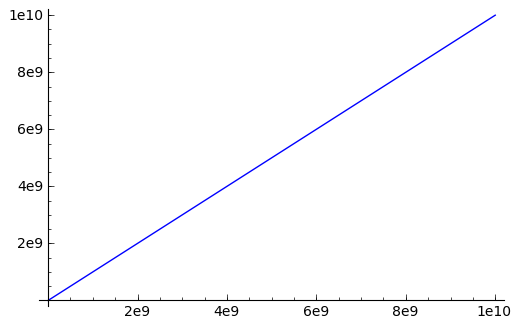
\includegraphics[height=4cm]{figures/x.png}}
	\hfill
	\subfloat[$10^x$]{\label{10hochx}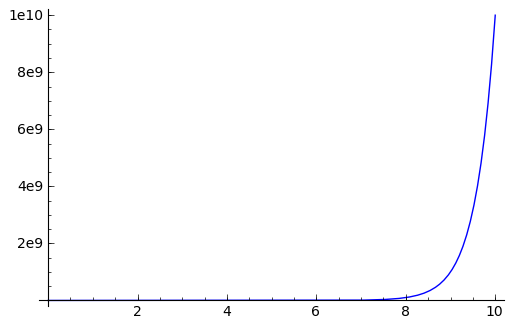
\includegraphics[height=4cm]{figures/10hochx.png}}
	\caption{Graph der Funktionen $x$ und $10^x$}
	\label{xund10hochx}
        \vskip +25pt 
\end{figure} 
% \\ nach end{figure} f�hrt zu  LaTeX Error: There's no line here to end.
% \vskip +30pt  nach end{figure} stellt den Space an den falschen Ort, da die Grafik eigenst�ndig gesetzt wird.
% \clearpage


\subsubsection*{Die Funktion $\ln{x}$}
Im Vergleich dazu betrachten wir die Funktion $\ln{x}$. 
Auf dem linken Bild von Abbildung \ref{lnxbis} auf Seite \pageref{lnxbis} wurde der
Definitionsbereich von $1$ bis $100$ gew�hlt. Das rechte Bild zeigt die Werte der
Funktion bis $10^{10}$.\\
Es ist gut zu erkennen, dass die Werte der Funktion $\ln{x}$ im Vergleich zu $x$
langsam wachsen. Dies verdeutlicht auch der Graph beider Funktionen in Abbildung
\ref{xundlnxundxdurchlnx} auf Seite \pageref{xundlnxundxdurchlnx}. Zudem wurde
in diesen Graphen auch die Funktion $\frac{x}{\ln{x}}$ eingezeichnet.

\begin{figure}[!htb]
	\centering
	\subfloat[ ]{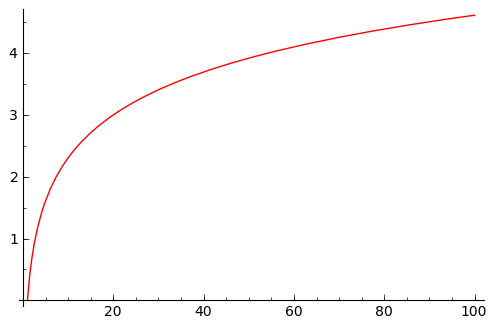
\includegraphics[height=4cm]{figures/lnxbis100.png}}
	\hfill
	\subfloat[ ]{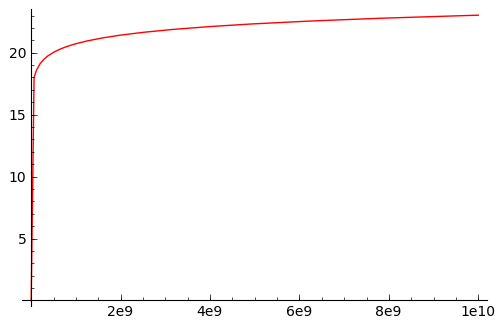
\includegraphics[height=4cm]{figures/lnxbis10hoch10.png}}
	\caption{Graph der Funktion $\ln{x}$ bis $100$ und bis $10^{10}$}
	\label{lnxbis}
        \vskip +25pt 
\end{figure}

\begin{figure}[!htb]
	\centering
	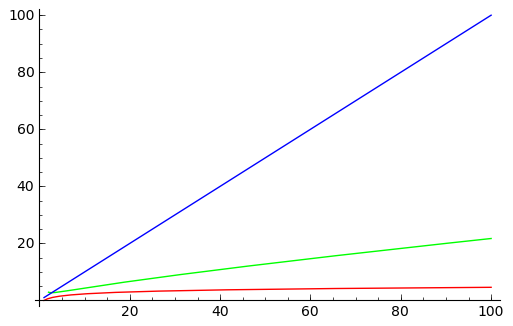
\includegraphics[height=4cm]{figures/xundlnxundxdurchlnx.png}
	\caption{Die Funktionen $x$ (blau), $\ln{x}$ (rot)
                 und $\frac{x}{\ln{x}}$ (gr�n)}
	\label{xundlnxundxdurchlnx}
        \vskip +15pt 
\end{figure} 


\subsubsection*{Die Funktion $PI(x) = \frac{x}{\ln{x}}$}
\index{PI(x), $\Pi(x)$}
Die Funktion $\frac{x}{\ln{x}}$ setzt sich also zusammen aus der Funktion $x$ im Z�hler und der im Verh�ltnis dazu sehr langsam wachsenden Funktion $\ln{x}$ im Nenner. Die Anzahl der Primzahlen kleiner oder gleich einer Zahl $x$ ist zwar verh�ltnism��ig klein im Vergleich zu $x$ selbst. Dennoch ist $\frac{x}{\ln{x}}$ eine wachsende Funktion. Dies wird auch deutlich in Abbildung \ref{xundlnxundxdurchlnx} auf Seite \pageref{xundlnxundxdurchlnx}.


\subsubsection*{Die Anzahl der Primzahlen in verschiedenen Intervallen}
\label{primes:_Appendix_subsubsection_NumberofPrimes-in-intervals}
Abbildung \ref{deltazehnxdurchlnxbis}
% auf Seite \pageref{deltazehnxdurchlnxbis}
veranschaulicht, wie sich die Anzahl der Primzahlen in den Intervallen
$[1, 10^x]$ und $[10^{x-1},10^{x}]$ entwickelt. Um es schneller
berechnen zu k�nnen, wird
nicht die exakte Anzahl (wie in den Tabellen in Kapitel \ref{s:primhfk})
benutzt, sondern der Wert der N�herungsfunktion.

Dabei werden pro Zehner-Exponenten zwei Balken gezeichnet:
$\frac{10^{x}}{\ln{10^{x}}}$ im Vergleich zu $\frac{10^{x}}{\ln{10^{x}}}-\frac{10^{x-1}}{\ln{10^{x-1}}}$:
Die linke Grafik f�r $x$ von $1$ bis $5$, und die rechte f�r $x$ von $1$ bis $10$, wobei x der Wert des Zehner-Exponenten ist.\\ 

Die blauen Balken geben an, wieviele Primzahlen es ingesamt bis $10^x$ gibt.
Die roten Balken zeigen, wieviele Primzahlen jeweils im letzten Intervall
$[10^{x-1},10^x]$ hinzukommen.
Dies verdeutlicht, dass die Anzahl der Primzahlen in Intervallen mit h�heren
Exponenten immer noch stark steigt. 

\begin{figure}[!htb]
	\centering
	\subfloat[ ]{\label{deltazehnxdurchlnxbis5}
                     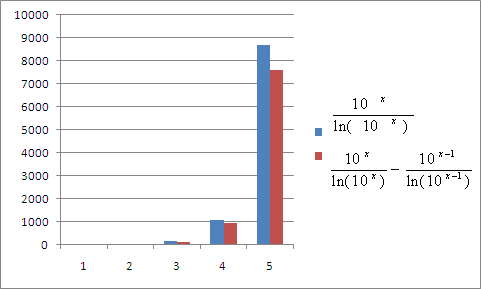
\includegraphics[height=4cm]{figures/deltazehnxdurchlnxbis5.png}}
	\hfill
	\subfloat[ ]{\label{deltazehnxdurchlnxbis10}
                     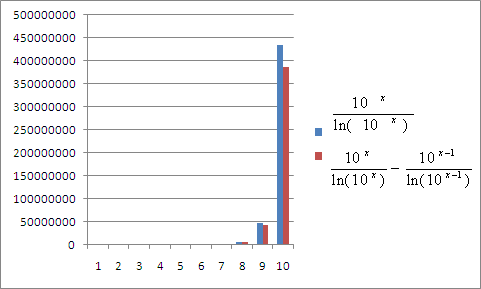
\includegraphics[height=4cm]{figures/deltazehnxdurchlnxbis10.png}}
	\caption{Anzahl der Primzahlen im Intervall $[1, 10^x]$ (blau) und im
         Intervall $[10^{x-1},10^x]$ (rot) (f�r verschiedene Exponenten $x$)}
	\label{deltazehnxdurchlnxbis}
\end{figure} 


Eine Tabelle mit den Anzahlen von Primzahlen in einigen ausgew�hlten Intervallen
finden Sie in Kapitel \ref{s:primhfk} auf Seite \pageref{s:primhfk}:
Z.B. liegen im Intervall $[1, 10^4]$ 1229 Primzahlen; davon befinden sich im
Intervall $[10^3, 10^4]$ 1229 - 168 = 1061 Primzahlen.

Theorie zum Primzahlsatz und zur Funktion PI(x) steht in Kapitel
\ref{l_Primes_Distrib-of-Primes}.



\begin{sagecode}
\begin{Verbatim}%
[fontsize=\footnotesize]

# Definition der Funktion f(x)=x und Plots f�r die Definitionsbereiche 0 bis 10^10 und 0 bis 100
sage: def f(x):return x
....:
sage: F=plot(f,(0,10^10))
sage: F.plot()

sage: F2=plot(f,(1,100))
sage: F2.plot()


# Definition der Funktion g(x)=10^x und Plot f�r den Definitionsbereich 0 bis 10
sage: def g(x): return 10^x
....:
sage: G=plot(g,(0,10))
sage: G.plot()


# Definition der Funktion h(x)=log(x) und Plots f�r die Definitionsbereiche 1 bis 100 und 1 bis 10^10
sage: def h(x): return log(x)
....:
sage: H=plot(h,(1,100),color="red")
sage: H.plot()

sage: H2=plot(h,(1,10^10),color="red")
sage: H2.plot()


# Definition der Funktion k(x)=x/log(x) und Plot f�r den Definitionsbereich 2 bis 100
sage: def k(x): return x/log(x)
....:
sage: K=plot(k,(2,100),color="green")
sage: K.plot()


# Plot der Funktionen f, k und h f�r den Definitionsbereich von 1 bzw. 2 bis 100
sage: F2+K+H


# Generieren der Daten f�r die Balkencharts ..........................
# Bestimmen der Anzahl der Primzahlen im Intervall [1,10]
sage: pari(10).primepi()-pari(1).primepi()
4

# Bestimmen der Anzahl der Primzahlen im Intervall [10^3,10^4]
sage: pari(10**4).primepi()-pari(10**3).primepi()
1061

# Bestimmen der Anzahl der Primzahlen im Intervall [10^8,10^9]
sage: pari(10**9).primepi()-pari(10**8).primepi()
45086079

# (ab 10^10: OverflowError: long int too large to convert)

\end{Verbatim}
\caption{Erzeugen der Graphen zu den drei Funktionen x, log(x) und x/log(x)}
\end{sagecode}




% ---------------------------------------------------------------------------
% ---------------------------------------------------------------------------
\clearpage
\newpage
\hypertarget{primes:_Appendix_Sage-Samples}{}
\section{Anhang: Beispiele mit SageMath}
% \section*{Appendix A: Beispiele mit SageMath}
% \addcontentsline{toc}{section}{Appendix A: Beispiele mit SageMath}
\label{primes:_Appendix_Sage-Samples}
\index{SageMath!Programmbeispiele}
\index{SageMath}

\noindent Der folgende Abschnitt enth�lt SageMath Source-Code zu den Inhalten aus
Kapitel~\ref{Label_Kapitel_Primes} (\glqq \nameref{Label_Kapitel_Primes}\grqq).


% ---------------------------------------------------------------------------
% \newpage
\subsection{Einfache Funktionen zu Primzahlen mit SageMath}
\index{SageMath}

In diesem Teil des Anhangs finden Sie den Quellcode f�r SageMath, mit dem man
einige einfache Berechnungen zu Primzahlen durchf�hren kann.%
\footnote{Siehe die SageMath-Dokumentation �ber Elementare Zahlentheorie
          \url{http://www.sagemath.org/doc/constructions/number_theory.html}.}

\begin{sagecode}
\begin{Verbatim}%
[fontsize=\footnotesize]

# Primzahlen (allgemeine Befehle)
# Die Menge der Primzahlen
sage: P=Primes(); P
Set of all prime numbers: 2, 3, 5, 7, ...

# Gibt die n�chste Primzahl aus
sage: next_prime(5)
7

# Gibt die Anzahl der Primzahlen <=x aus
sage: pari(10).primepi()
4

# Gibt die ersten x Primzahlen aus
sage: primes_first_n(5)
[2, 3, 5, 7, 11]

# Gibt die Primzahlen in einem Interval aus
sage: list(primes(1,10))
[2, 3, 5, 7]

\end{Verbatim}
\caption{Einige einfache Funktionen zu Primzahlen}
\end{sagecode}



% ---------------------------------------------------------------------------
\newpage
\subsection{Primalit�ts-Check der von einer quadratischen Funktion erzeugten Zahlen}
\index{SageMath}

In diesem Anhang finden Sie den Quellcode f�r SageMath, mit dem man
z.B.\ pr�fen kann, ob die von der Funktion $f(n) = n^2 - 9n + 61$ 
erzeugten Zahlen prim sind. 
Der Quellcode definiert eine Funktion namens \verb!quadratic_prime_formula()!,
die die folgenden drei Argumente hat:
\begin{itemize}
\item \verb!start! --- Ein nat�rliche Zahl, die die Untergrenze der Folge
  $\texttt{start}, \texttt{start} + 1,
  \texttt{start} + 2, \dots, \texttt{end} - 1, \texttt{end}$ darstellt.

\item \verb!end! --- Ein nat�rliche Zahl, die die Obergrenze der Folge
  $\texttt{start}, \texttt{start} + 1,
  \texttt{start} + 2, \dots, \texttt{end} - 1, \texttt{end}$ darstellt.

\item \verb!verbose! --- (Standardwert: \verb!True!) Ein Schalter, der festlegt,
  ob f�r jede erzeugte Einzelzahl $f(n)$ eine Ausgabe zur Primalit�t erfolgen soll.
\end{itemize}

\noindent Eine sinnvolle �nderung dieses Codes besteht darin, eine andere Funktion anzugeben,
deren Funktionswerte auf Primalit�t gepr�ft werden sollen.


\begin{sagecode}
\begin{Verbatim}%
[fontsize=\footnotesize]
def quadratic_prime_formula(start, end, verbose=True):
    print "N -- N^2 - 9*N + 61"
    P = 0 # the number of primes between start and end
    for n in xrange(start, end + 1):
        X = n^2 - 9*n + 61
        if is_prime(X):
            P += 1
            if verbose:
                 print str(n) + " -- " + str(X) + " is prime"
        else:
            if verbose:
                 print str(n) + " -- " + str(X) + " is NOT prime"
    print "Number of primes: " + str(P)
    print "Percentage of primes: " + str(float((P * 100) / (end - start + 1)))
\end{Verbatim}
\caption{Testen der Primalit�t von Funktionswerten, erzeugt von einer quadratischen Funktion}
\end{sagecode}

\vspace{12pt}
Mit dem folgenden Funktionsaufruf berechnen wir die Werte von $f(n) = n^2 - 9n + 61$
f�r $n = 0, 1, 2, \dots, 50$ und verifizieren die Primalit�t der erzeugten Funktionswerte:

\begin{Verbatim}%
[fontsize=\footnotesize]
sage: quadratic_prime_formula(0, 50)
 N -- N^2 - 9*N + 61
0 -- 61 is prime
1 -- 53 is prime
2 -- 47 is prime
3 -- 43 is prime
4 -- 41 is prime
5 -- 41 is prime
6 -- 43 is prime
7 -- 47 is prime
8 -- 53 is prime
9 -- 61 is prime
10 -- 71 is prime
11 -- 83 is prime
12 -- 97 is prime
13 -- 113 is prime
14 -- 131 is prime
15 -- 151 is prime
16 -- 173 is prime
17 -- 197 is prime
18 -- 223 is prime
19 -- 251 is prime
20 -- 281 is prime
21 -- 313 is prime
22 -- 347 is prime
23 -- 383 is prime
24 -- 421 is prime
25 -- 461 is prime
26 -- 503 is prime
27 -- 547 is prime
28 -- 593 is prime
29 -- 641 is prime
30 -- 691 is prime
31 -- 743 is prime
32 -- 797 is prime
33 -- 853 is prime
34 -- 911 is prime
35 -- 971 is prime
36 -- 1033 is prime
37 -- 1097 is prime
38 -- 1163 is prime
39 -- 1231 is prime
40 -- 1301 is prime
41 -- 1373 is prime
42 -- 1447 is prime
43 -- 1523 is prime
44 -- 1601 is prime
45 -- 1681 is NOT prime
46 -- 1763 is NOT prime
47 -- 1847 is prime
48 -- 1933 is prime
49 -- 2021 is NOT prime
50 -- 2111 is prime
Number of primes: 48
Percentage of primes: 94.1176470588
\end{Verbatim}

\noindent Die Statistik in den letzten beiden Zeilen der Ausgabe zeigt, dass
$f(n)$ 48 Primzahlen erzeugt f�r $0 \leq n \leq 50$, was ca. 94\% der von
$f(n)$ erzeugten Werte darstellt.\\

Bei l�ngeren Sequenzen ist die Einzelausgabe der erzeugten Zahl und ihrer Primalit�t
ziemlich unpraktisch. Deshalb wird in der folgenden SageMath-Session nur die Statistik am
Ende ausgegeben (indem man den Verbose-Parameter auf False setzt): die Gesamtzahl und
der prozentuale Anteil der Primzahlen, die von
$f(n)$ im Bereich $0 \leq n \leq 1000$ erzeugt wurde.

\begin{Verbatim}%
[fontsize=\footnotesize]
sage: quadratic_prime_formula(0, 1000, verbose=False)
N -- N^2 - 9*N + 61
Number of primes: 584
Percentage of primes: 58.3416583417
\end{Verbatim}









% --------------------------------------------------------------------------
\newpage
\begin{thebibliography}{99999}
\addcontentsline{toc}{section}{Literaturverzeichnis}


\bibitem[Aaronson2003]{pr:Aaronson2003} \index{Aaronson 2003}
    Scott Aaronson, \\
    {\em The Prime Facts: From Euclid to AKS}, \\
    % veraltete Seite: http://www.cs.berkeley.edu/~aaronson/prime.ps
    \url{http://www.scottaaronson.com/writings/prime.pdf} \\
    Dieses sch�ne Paper wurde mir erst nach Vollendung der ersten Fassung
    dieses Artikels bekannt: Es bietet ebenfalls einen einfachen, didaktisch 
    gut aufbereiteten und trotzdem nicht oberfl�chlichen Einstieg 
    in dieses Thema (ist nur in Englisch verf�gbar).

% already defined in elementaryNumberTheory.inc -> 2 davor
\bibitem[Bartholome1996]{pr:2Bartholome1996}  \index{Bartholome 1996}
    A. Bartholom\'e, J. Rung, H. Kern, \\
    {\em Zahlentheorie f�r Einsteiger}, Vieweg, 1995, 2. Auflage 1996.

\bibitem[Blum1999]{pr:Blum1999} \index{Blum 1999}
    W. Blum, \\
    {\em Die Grammatik der Logik}, dtv, 1999.

\bibitem[Bundschuh1998]{pr:Bundschuh1998} \index{Bundschuh 1998}
    Peter Bundschuh, \\
    {\em Einf�hrung in die Zahlentheorie}, Springer, 1988, 4. Auflage 1998.

\bibitem[Crandell2001]{pr:Crandell2001} \index{Crandell 2001} \index{Pomerance 2001}
    Richard Crandell, Carl Pomerance, \\
    {\em Prime Numbers. A Computational Perspective}, Springer, 2001.

\bibitem[Doxiadis2000]{pr:Dioxadis2000}
    Apostolos Doxiadis, \\
    {\em Onkel Petros und die Goldbachsche Vermutung}, \\
    Bloomsbury 2000 (deutsch bei L�bbe 2000 und bei BLT als Taschenbuch 2001).

\bibitem[Graham1989]{pr:Graham1989} \index{Graham 1989}
    R.E. Graham, D.E. Knuth, O. Patashnik, \\
    {\em Concrete Mathematics}, Addison-Wesley, 1989.

\bibitem[Klee1997]{pr:Klee1997} \index{Klee 1997}
    V. Klee, S. Wagon, \\
    {\em Ungel�ste Probleme in der Zahlentheorie und der
    Geometrie der Ebene}, \\ Birkh�user Verlag, 1997.

\bibitem[Knuth1981]{pr:Knuth1981} \index{Knuth 1981}
    Donald E. Knuth, \\
    {\em The Art of Computer Programming, vol 2: Seminumerical
    Algorithms}, \\ Addison-Wesley, 1969, 2nd edition 1981.

\bibitem[Lorenz1993]{pr:Lorenz1993} \index{Lorenz 1993}
    F. Lorenz, \\
    {\em Algebraische Zahlentheorie}, BI Wissenschaftsverlag, 1993.

\bibitem[Oppliger2011]{pr:Oppliger2011} \index{Oppliger 2011}
    Rolf Oppliger \\
    {\em Contemporary Cryptography, Second Edition},
    Artech House, 2011, \\
    \url{http://books.esecurity.ch/cryptography2e.html}.

\bibitem[Padberg1996]{pr:Padberg1996} \index{Padberg 1996}
    Friedhelm Padberg, \\
    {\em Elementare Zahlentheorie}, 
    Spektrum Akademischer Verlag, 1988, 2. Auflage 1996.

\bibitem[Pieper1983]{pr:Pieper1983} \index{Pieper 1983}
    H. Pieper, \\
    {\em Zahlen aus Primzahlen}, 
    Verlag Harri Deutsch, 1974, 3. Auflage 1983.

\bibitem[Rempe2009]{pr:Rempe2009}  \index{Rempe 2009}
    L. Rempe, R. Waldecker, \\
    {\em Primzahltests f�r Einsteiger}, Vieweg+Teubner, 2009. \\
    Dieses Buch entstand aus einem Kurs an der "`Deutschen Sch�lerakademie"'.
    Es stellt den AKS-Beweis vollst�ndig dar, ohne mathematisches Vorwissen zu
    zu erwarten.

\bibitem[Richstein1999]{pr:Richstein1999} \index{Richstein 1999}
    J. Richstein, \\
    {\em Verifying the Goldbach Conjecture up to $4*10^{14},$} 
    Mathematics of Computation 70, 2001, S. 1745-1749. 

\bibitem[Scheid1994]{pr:Scheid1994} \index{Scheid 1994}
    Harald Scheid, \\ 
    {\em Zahlentheorie}, BI Wissenschaftsverlag, 2. Auflage 1994.

%already defined in elementaryNumberTheory.inc -> 2 davor
\bibitem[Schneier1996]{pr:Schneier1996p} \index{Schneier 1996}
    Bruce Schneier, \\
    {\em Applied Cryptography, Protocols, Algorithms, and Source Code in C},\\
    Wiley and Sons, 2nd edition 1996.

\bibitem[Schroeder1999]{pr:Schroeder1999} \index{Schroeder 1999}
    M.R. Schroeder, \\
    {\em Number Theory in Science and Communication}, \\
    Springer, 1984, 3rd edition 1997, Corrected Printing 1999.

\bibitem[Schwenk1996]{pr:Schwenk1996} \index{Schwenk 1996}
    J. Schwenk \\
    {\em Conditional Access},
    in taschenbuch der telekom praxis, 1996, \\
    Hrgb. B. Seiler, Verlag Schiele und Sch�n, Berlin.

\bibitem[Shoup2005]{pr:Shoup2005} \index{Shoup 2005}
    Victor Shoup \\
    {\em A Computational Introduction to Number Theory and Algebra},
    Cambridge University Press, 2005, \\
    \url{http://shoup.net/ntb/}.

\bibitem[Tietze1973]{pr:Tietze1973} \index{Tietze 1973}
    H. Tietze, \\
    {\em Gel�ste und ungel�ste mathematische Probleme}, 
    Verlag C.H. Beck, 1959, 6. Auflage 1973.

\end{thebibliography}


% --------------------------------------------------------------------------
\newpage
\chapter*{Web-Links}\addcontentsline{toc}{section}{Web-Links}

\begin{enumerate}
   \item GIMPS (Great Internet Mersenne-Prime Search) 
      \index{Mersenne!Mersenne-Primzahl} \\
         www.mersenne.org ist die Homepage des GIMPS-Projekts, \index{GIMPS} \\
      \url{http://www.mersenne.org/prime.htm}

\item Die Proth Search Page mit dem Windows-Programm von Yves Gallot \\
      \url{http://www.utm.edu/research/primes/programs/gallot/index.html}

\item Verallgemeinerte Fermat-Primzahlen-Suche \\
      \url{http://primes.utm.edu/top20/page.php?id=12}

\item Verteilte Suche nach Teilern von Fermatzahlen \\
      \url{http://www.fermatsearch.org/}

\item An der Universit�t von Tennessee findet man umfangreiche 
      Forschungsergebnisse �ber Primzahlen. \\
      \url{http://www.utm.edu/}

\item Den besten �berblick zu Primzahlen (weil sehr aktuell und vollst�ndig)
      bieten m.E.  ~\glqq The Prime Pages\grqq~ von Professor Chris Caldwell.
      \index{Caldwell, Chris} \\
      \url{http://www.utm.edu/research/primes}

\item Beschreibungen u.a. zu Primzahltests \\
      \url{http://www.utm.edu/research/primes/mersenne.shtml} \\
      \url{http://www.utm.edu/research/primes/prove/index.html}

\item Ausgabe der $n$-ten Primzahl P(n)\\
      \url{http://www.utm.edu/research/primes/notes/by_year.html}

\item Der Supercomputerhersteller SGI Cray Research besch�ftigte nicht
      nur hervorragende Mathematiker, sondern benutzte die Primzahltests
      auch als Benchmarks f�r seine Maschinen. \\
      \url{http://www.isthe.com/chongo/tech/math/prime/prime_press.html}

\item Das Cunningham-Projekt, \index{Cunningham-Projekt}\\ 
      \url{http://www.cerias.purdue.edu/homes/ssw/cun/}

\item \url{http://www.eff.org/awards/coop}

% \item \url{http://www.informatik.tu-darmstadt.de/TI/LiDIA/}

\item \url{http://www.math.Princeton.EDU/~arbooker/nthprime.html}

\item Goldbach conjecture verification project von Tom�s Oliveira e Silva,
      \index{Goldbach-Projekt}\\ 
      \url{http://sweet.ua.pt/tos/goldbach.html}

\item \url{http://www.mathematik.ch/mathematiker/goedel.html}

% Info: http://www.mathematik.ch/mathematiker/Goldbachsche_Vermutung.php
% tot: \item \url{http://www.informatik.uni-giessen.de/staff/richstein/de/Goldbach.html}
% tot  \item \url{http://www.mscs.dal.ca/~dilcher/golbach/index.html}
% tot        \url{http://www.mscs.dal.ca/~joerg/res/g-en.html}


\end{enumerate}


\vskip +10 pt
% --------------------------------------------------------------------------(5\cdot2^7 - 1)(5^2\cdot2^14 + 1)
\section*{Dank} \addcontentsline{toc}{section}{Dank}
F�r das sehr konstruktive Korrekturlesen der ersten Versionen
dieses Artikels: Hr. Henrik Koy und Hr. Roger Oyono.





% Local Variables:
% TeX-master: "../script-de.tex"
% End:(5\cdot2^7 - 1)(5^2\cdot2^14 + 1)(5\cdot2^7 - 1)(5^2\cdot2^14 + 1)

% $Id: numbertheory.tex 3715 2016-04-10 18:18:55Z esslinger $
% ..........................................................................
% --------------------------------------------------------------------------
% ++++++++++++++++++++++++++++++++++++++++++++++++++++++++++++++++++++++++++
%              E l e m e n t a r e  Z a h l e n t h e o r i e
% ~~~~~~~~~~~~~~~~~~~~~~~~~~~~~~~~~~~~~~~~~~~~~~~~~~~~~~~~~~~~~~~~~~~~~~~~~~

%\def\QM {{,\kern -0.9 pt ,}}
\setcounter{satz}{0}
\setcounter{definition}{0}

\hypertarget{Chapter_ElementaryNT}{}
\chapter{Einf�hrung in die elementare Zahlentheorie mit Beispielen}
\label{Chapter_ElementaryNT}
(Bernhard Esslinger, Juli 2001; Updates: Nov. 2001, Juni 2002, Mai 2003,
 Mai 2005, M�rz 2006, Juni 2007, Juli 2009, Jan. 2010, Aug. 2013) \\

Diese \glqq Einf�hrung\grqq~bietet einen Einstieg f�r mathematisch
Interessierte. Erforderlich sind nicht mehr Vorkenntnisse als die, die im
Grundkurs Mathematik am Gymnasium vermittelt werden.\par
Wir haben uns bewusst an \glqq Einsteigern\grqq~ und \glqq Interessenten\grqq~
orientiert, und nicht an den Gepflogenheiten mathematischer Lehrb�cher, die
auch dann \glqq Einf�hrung\grqq~ genannt werden, wenn sie schon auf der 5. Seite
nicht mehr auf Anhieb zu verstehen sind und sie eigentlich den Zweck haben, dass
man danach auch spezielle Monographien zu dem Thema lesen k�nnen soll.



% ++++++++++++++++++++++++++++++++++++++++++++++++++++++++++++++++++++++++++
\section{Mathematik und Kryptographie}
Ein gro�er Teil der modernen, asymmetrischen Kryptographie beruht auf 
mathematischen Erkenntnissen -- auf den Eigenschaften (\glqq Gesetzen\grqq)
ganzer Zahlen, die in der elementaren \index{Zahlentheorie!elementare}
Zahlentheorie untersucht werden. \glqq Elementar\grqq\ bedeutet hier, 
dass die zahlentheoretischen Fra"-ge"-stellungen im wesentlichen
in der Menge der nat�rlichen und der ganzen Zahlen durchgef�hrt werden.

Weitere mathematische Disziplinen, die heute in der Kryptographie 
Verwendung finden, sind 
(vgl. \cite[S. 2]{nt:Bauer1995}, \cite[Seite 3]{nt:Bauer2000}) :
\begin{itemize}
    \item Gruppentheorie\index{Gruppe}
    \item Kombinatorik
    \item Komplexit�tstheorie\index{Komplexit�t}
    \item Stochastik (Ergodentheorie)
    \item Informationstheorie.
\end{itemize}

Die Zahlentheorie oder Arithmetik (hier wird mehr der Aspekt des Rechnens
mit Zahlen betont) wurde von Gauss\footnote{%
  Carl Friedrich Gauss, deutscher Mathematiker und Astronom,
  30.4.1777$-$23.2.1855.
}
\index{Gauss, Carl Friedrich}
als besondere mathematische Disziplin begr�ndet. Zu ihren elementaren
Gegenst�nden geh�ren: gr��ter gemeinsamer Teiler\footnote{%
Auf ggT\index{ggT}, englisch gcd (greatest common divisor), geht dieser
Artikel in Anhang~\ref{nt:NumberTheory_Appendix_GCD} ein.
} (ggT), Kongruenzen (Restklassen), Faktorisierung, Satz von Euler-Fermat und
primitive Wurzeln. Kernbegriff sind jedoch die Primzahlen und ihre
multiplikative Verkn�pfung.

Lange Zeit galt gerade die Zahlentheorie als Forschung pur, als
Paradebeispiel f�r die Forschung im Elfenbeinturm. Sie erforschte die
\glqq geheimnisvollen Gesetze im Reich der Zahlen\grqq~und gab Anlass zu
philosophischen Er�rterungen, ob sie beschreibt, was �berall in der Natur
schon da ist, oder ob sie ihre Elemente (Zahlen, Operatoren, Eigenschaften)
nicht k�nstlich konstruiert.

Inzwischen wei� man, dass sich zahlentheoretische Muster �berall in der Natur
finden. Zum Beispiel verhalten sich die Anzahl der links- und der
rechtsdrehenden Spiralen einer Sonnenblume zueinander wie zwei
aufeinanderfolgende\index{Fibonacci} Fibonacci-Zahlen\footnote{%
Die Folge der Fibonacci-Zahlen $(a_i)_{i \in \mathbb{N}}$ ist definiert durch
die \glqq rekursive\grqq~Vorschrift $a_1 := a_2 := 1$ und f�r alle Zahlen  $n=1,2,3,\cdots$ definiert man 
$a_{n+2} := a_{n+1}+a_n$.  Zu dieser historischen Folge gibt es viele interessante 
Anwendungen in der Natur (siehe z.B. \cite[S. 290 ff]{nt:Graham1994}\index{Graham 1994}
oder die Web-Seite von \hyperlink{knott}{Ron Knott:}\index{Knott, Ron}
Hier dreht sich alles um Fibonacci-Zahlen). 
Die Fibonacci-Folge\index{Fibonacci} ist gut verstanden und wird heute als
wichtiges Werkzeug in der Mathematik benutzt.
}, also z.B.  wie  $21 : 34$.

Au�erdem wurde sp�testens mit den zahlentheoretischen Anwendungen der
modernen Kryptographie klar, dass eine jahrhundertelang als theoretisch
geltende Disziplin praktische Anwendung findet, nach deren Experten heute
eine hohe Nachfrage auf dem Arbeitsmarkt besteht.

Anwendungen der (Computer-)Sicherheit bedienen sich heute der Kryptographie,
weil Kryptographie als mathematische Disziplin einfach besser und
beweisbarer ist als alle im Laufe der Jahrhunderte erfundenen \glqq kreativen\grqq~
Verfahren der Substitution und besser als alle ausgefeilten physischen
Techniken wie beispielsweise beim Banknotendruck \cite[S. 4]{nt:Beutelspacher1996}.

In diesem Artikel werden in einer leicht verst�ndlichen Art die
grundlegenden Erkenntnisse der elementaren Zahlentheorie anhand vieler
Beispiele vorgestellt -- auf Beweise wird (fast) vollst�ndig verzichtet
(diese finden sich in den mathematischen Lehrb�chern).

Ziel ist nicht die umfassende Darstellung der zahlentheoretischen Erkenntnisse,
sondern das Aufzeigen der wesentlichen Vorgehensweisen. Der Umfang des Stoffes
orientiert sich daran, das RSA-Verfahren\index{RSA} verstehen und anwenden
zu k�nnen.

Dazu wird sowohl an Beispielen als auch in der Theorie erkl�rt, wie man in
endlichen Mengen rechnet und wie dies in der Kryptographie Anwendung findet.
Insbesondere wird auf die klassischen Public-Key-Verfahren Diffie-Hellman
\index{Diffie-Hellman} (DH) und RSA\index{RSA} eingegangen.

Es war mir wichtig, fundierte Aussagen zur Sicherheit des RSA-Verfahrens zu
machen, und f�r m�glichst alle Beispiele SageMath-Code anzugeben.


% ++++++++++++++++++++++++++++++++++++++++++++++++++++++++++++++++++++++++++
\newpage
\begin{ctsquote}
Die Mathematik ist die K�nigin der Wissenschaften, die Zahlentheorie aber
ist die K�nigin der Mathematik.
\caption{Carl Friedrich Gauss}\index{Gauss, Carl Friedrich}
\end{ctsquote}

% ++++++++++++++++++++++++++++++++++++++++++++++++++++++++++++++++++++++++++
\section{Einf�hrung in die Zahlentheorie}
\index{Zahlentheorie!Einf�hrung} 

Die Zahlentheorie entstand aus Interesse an den positiven ganzen Zahlen $1,
2, 3, 4, \cdots ,$ die auch als die Menge der \index{Zahlen!nat�rliche}
{\em nat�rlichen Zahlen} $\mathbb{N}$ bezeichnet
werden. Sie sind die ersten mathematischen Konstrukte der menschlichen
Zivilisation. Nach Kronecker\footnote{%
Leopold Kronecker, deutscher Mathematiker, 7.12.1823$-$29.12.1891.
}
\index{Kronecker, Leopold} hat sie der liebe Gott geschaffen, 
nach Dedekind\footnote{Julius Wilhelm Richard Dedekind,
deutscher Mathematiker, 06.10.1831$-$12.02.1916.
}
\index{Dedekind, Julius} der menschliche Geist.
Das ist je nach Weltanschauung ein unl�sbarer Widerspruch oder
ein und dasselbe.

Im Altertum gab es keinen Unterschied zwischen Zahlentheorie und
Numerologie, die einzelnen Zahlen mystische Bedeutung zuma�. So wie sich
w�hrend der Renaissance (ab dem 14. Jahrhundert) die Astronomie allm�hlich
von der Astrologie und die Chemie von der Alchemie l�ste, so lie� auch die
Zahlentheorie die Numerologie hinter sich.

Die Zahlentheorie faszinierte schon immer Amateure wie auch professionelle
Mathematiker. Im Unterschied zu anderen Teilgebieten der Mathematik k�nnen
viele der Probleme und S�tze auch von Laien verstanden werden, andererseits
widersetzten sich die L�sungen zu den Problemen und die Beweise zu den S�tzen
oft sehr lange den Mathematikern. Es ist also leicht, gute Fragen zu stellen,
aber es ist ganz etwas anderes, die Antwort zu finden. Ein Beispiel daf�r ist
der sogenannte letzte (oder gro�e) Satz von Fermat.\footnote{Thema der
   Schul-Mathematik ist der Satz von Pythagoras\index{Pythagoras!Satz von}:
   Den Sch�lern wird beigebracht, dass in einem ebenen, rechtwinkligen Dreieck
   gilt: $a^2 + b^2 = c^2$, wobei $a, b$ die Schenkell�ngen sind und 
   c die L�nge der Hypothenuse ist.
   Fermats ber�hmte Behauptung war, dass f�r $a,b,c \in \mathbb{N}$ und
   f�r ganzzahlige Exponenten $n > 2$ immer die Ungleichheit
   $a^n + b^n \not= c^n$ gilt.  Leider fand \index{Fermat!letzter Satz}
   Fermat auf dem Brief, wo er die Behauptung aufstellte, nicht gen�gend
   Platz, um den Satz zu beweisen. Der Satz konnte erst �ber 300 Jahre sp�ter
   bewiesen werden \cite[S. 433-551]{nt:Wiles1994}. \index{Wiles, Andrew}
}

Bis zur Mitte des 20. Jahrhunderts wurde die Zahlentheorie als das reinste
Teilgebiet der Mathematik angesehen -- ohne Verwendung in der wirklichen Welt.
Mit dem Aufkommen der Computer und der digitalen Kommunikation �nderte sich
das: die Zahlentheorie konnte einige unerwartete Antworten f�r reale
Aufgabenstellungen liefern. Gleichzeitig halfen die Fortschritte in der EDV,
dass die Zahlentheoretiker gro�e Fortschritte machten im Faktorisieren gro�er
Zahlen, in der Bestimmung neuer Primzahlen, im Testen von (alten)
Vermutungen und beim L�sen bisher unl�sbarer numerischer Probleme.

Die moderne Zahlentheorie \index{Zahlentheorie!moderne} besteht aus Teilgebieten wie
\begin{itemize}
    \item Elementare Zahlentheorie
    \item Algebraische Zahlentheorie
    \item Analytische Zahlentheorie
    \item Geometrische Zahlentheorie
    \item Kombinatorische Zahlentheorie
    \item Numerische Zahlentheorie und
    \item Wahrscheinlichkeitstheorie.
\end{itemize}

Die verschiedenen Teilgebiete besch�ftigen sich alle mit Fragestellungen zu
den ganzen Zahlen (positive und negative ganze Zahlen und die Null), gehen
diese jedoch mit verschiedenen Methoden an.

Dieser Artikel besch�ftigt sich nur mit dem Teilgebiet der elementaren
Zahlentheorie.


% --------------------------------------------------------------------------
\vskip +40 pt
\subsection{Konvention}
\index{Konvention}
Wird nichts anderes gesagt, gilt: 
\begin{itemize}
\item Die Buchstaben $a, b, c, d, e, k, n, m, p, q$ stehen f�r ganze Zahlen.
\item Die Buchstaben $i$ ~\mbox{und} ~$j$ stehen f�r nat�rliche Zahlen. 
\item Der Buchstabe $p$ steht stets f�r eine Primzahl.
\item Die Mengen $\mathbb{N} = \{ 1, 2, 3, \cdots \}$ und $\mathbb{Z} =\{ \cdots, -3, -2, -1, 0, 1, 2, 3, \cdots \}$ 
sind die {\em nat�rlichen} und die {\em ganzen} Zahlen.
\end{itemize}



% ++++++++++++++++++++++++++++++++++++++++++++++++++++++++++++++++++++++++++
%\vskip +40 pt
\newpage
\begin{ctsquote}
Das ist nicht Zauberei, das ist Logik, ein R�tsel.
Viele von den gr��ten Zauberern haben keine Unze Logik im Kopf.
\caption[Joanne K. Rowling]{Joanne K. Rowling\footnotemark}\index{Rowling, Joanne}
\end{ctsquote}
\addtocounter{footnote}{0}\footnotetext{Joanne K. Rowling,~\glqq Harry Potter
und der Stein der Weisen\grqq, Carlsen, (c) 1997, Kapitel ~\glqq Durch die Fallt�r\grqq, S. 310, Hermine.}


% ++++++++++++++++++++++++++++++++++++++++++++++++++++++++++++++++++++++++++
\section[Primzahlen und der erste Hauptsatz der elementaren Zahlentheorie]
        {Primzahlen und der erste Hauptsatz der elementaren Zah"-lentheorie}
\index{Zahlentheorie!elementare}
Viele der Fragestellungen in der elementaren Zahlentheorie besch�ftigen sich mit Primzahlen (siehe Kapitel~\ref{Label_Kapitel_Primes}).

Jede ganze Zahl hat Teiler oder Faktoren. Die Zahl 1 hat nur einen, n�mlich
sich selbst. Die Zahl 12 hat die sechs Teiler 1, 2, 3, 4, 6 und 12.\footnote{%
Aufgrund der gro�en Teilerzahl von 12 findet sich diese Zahl -- und Vielfache
dieser Zahl -- oft im Alltag wieder:
Die 12 Stunden-Skala der Uhr, die 60 Minuten einer Stunde, die 360 Grad-Skala
der Winkelmessung, usw. Teilt man diese Skalen in Bruchteile auf, so ergeben
in vielen F�llen die Br�che ganze Zahlen. Mit diesen kann 
man im Kopf einfacher rechnen als mit gebrochenen Zahlen.
}
Viele Zahlen sind nur teilbar durch sich selbst und durch 1. Bez�glich der
Multiplikation sind dies die \glqq Atome\grqq~im Bereich der Zahlen.

\index{Primzahl}
\begin{definition}\label{def-zth-prime} 
{\bf Primzahlen} sind nat�rliche Zahlen gr��er als $1$, die nur durch $1$ und sich
selbst teilbar sind.
\end{definition}

Per Definition ist $1$ keine Primzahl.

Schreibt man die Primzahlen in aufsteigender Folge (Primzahlenfolge), so
ergibt sich
$$2,~ 3,~ 5,~ 7,~ 11, ~13,~ 17,~ 19, ~23, ~29, ~31, ~37,~ 41,~ 43,~ 47,~ 53, ~59, ~61, ~67, ~71,
~73, ~79, ~83, ~89, ~97, \cdots.$$

Unter den ersten $100$ Zahlen gibt es genau $25$ Primzahlen. Danach nimmt ihr
prozentualer Anteil ab, wird aber nie Null.

Primzahlen treten als ganze Zahlen nicht selten auf. Allein im letzten
Jahrzehnt waren drei Jahre prim: $1993, 1997$ und $1999$. W�ren sie selten,
k�nnte die Kryptographie auch nicht so mit ihnen arbeiten, wie sie es tut.

Primzahlen k�nnen nur auf eine einzige (\glqq triviale\grqq) Weise zerlegt werden:
\begin{eqnarray*}
5 & = & 1 * 5 \nonumber \\
17 & =  & 1 * 17 \nonumber \\
1.013 &  = & 1 * 1013 \nonumber \\
1.296.409 & = & 1 * 1.296.409. \nonumber
\end{eqnarray*}

\index{Zahlen!zusammengesetzte}
\begin{definition}\label{def-zth-composite} 
Nat�rliche Zahlen gr��er $1$, die keine Primzahlen sind, hei�en
{\bf zusammengesetzte Zahlen}: Diese haben mindestens zwei von $1$ verschiedene
Faktoren.
\end{definition}


\begin{example}{ Primfaktorzerlegung\index{Primfaktor!Zerlegung} solcher Zahlen:}
\begin{eqnarray*}
4 & = & 2*2  \nonumber \\
6 & = & 2*3  \nonumber \\
91 & = & 7*13  \nonumber \\
161 & = & 7*23  \nonumber \\
767 & = & 13*59  \nonumber \\
1.029 & = & 3 * 7^3  \nonumber \\
5.324 & = & 22 * 11^3.  \nonumber 
\end{eqnarray*}

\begin{satz}\label{thm-zth-cnum}
Jede zusammengesetzte Zahl $a$ besitzt einen kleinsten Teiler gr��er
als $1$. Dieser Teiler ist eine Primzahl $p$ und kleiner oder gleich der Quadratwurzel
aus $a$.
\end{satz}
\end{example}
Aus den Primzahlen lassen sich alle ganzen Zahlen gr��er als $1$
zusammensetzen -- und das sogar in einer {\em eindeutigen} Weise.

Dies besagt \index{Zahlentheorie!Hauptsatz} der 1. {\em Hauptsatz der Zahlentheorie} (= Hauptsatz der elementaren
Zahlentheorie = fundamental theorem of arithmetic = fundamental building
block of all positive integers). Er wurde das erste Mal pr�zise von Carl
Friedrich Gauss in seinen Disquisitiones Arithmeticae (1801) formuliert. 
\index{Zahlentheorie!Hauptsatz}  \index{Gauss, Carl Friedrich}

\begin{satz}{\bf Gauss 1801}\label{thm-zth-mthm}
Jede nat�rliche Zahl $a$ gr��er als $1$ l�sst sich als Produkt von
Primzahlen schreiben. Sind zwei solche Zerlegungen $a = p_1*p_2*\cdots*p_n = q_1*q_2*\cdots*q_m$ gegeben, dann
gilt nach eventuellem Umsortieren $n = m$ und f�r alle $i$: $p_i = q_i$.
\end{satz}

In anderen Worten: Jede nat�rliche Zahl au�er der $1$ l�sst sich auf genau eine
Weise als Produkt von Primzahlen schreiben, wenn man von der Reihenfolge der
Faktoren absieht. Die Faktoren sind also eindeutig (die \glqq Expansion in
Faktoren\grqq~ist eindeutig)!

Zum Beispiel ist $60 = 2*2*3*5 = 2^2*3*5$. Und das ist --- bis auf eine
ver�nderte Reihenfolge der Faktoren --- die einzige M�glichkeit, die Zahl $60$
in Primfaktoren\index{Primfaktor} zu zerlegen.

Wenn man nicht nur Primzahlen als Faktoren zul�sst, gibt es mehrere
M�glichkeiten der Zerlegung in Faktoren und die {\em Eindeutigkeit} (uniqueness)
geht verloren:
$$60 = 1*60 = 2*30 = 4*15 = 5*12 = 6*10 = 2*3*10 = 2*5*6 = 3*4*5 = \cdots$$
Der 1. Hauptsatz ist nur scheinbar selbstverst�ndlich. Man kann viele andere
Zahlenmengen\footnote{%
Diese Mengen werden speziell aus der Menge der nat�rlichen Zahlen gebildet.
Ein Beispiel findet sich in diesem \hyperlink{uniqueness}{Skript}
auf Seite~\pageref{thm-pz-euklid} %eigentlich \pageref{remFundTheoOfArithm},
%aber hyperref ist buggy
am Ende von Kapitel~\ref{primesinmath}.
}
konstruieren, bei denen eine multiplikative Zerlegung in die Primfaktoren
dieser Mengen {\em nicht} eindeutig ist.

F�r eine mathematische Aussage ist es deshalb nicht nur wichtig, f�r welche
Operation sie definiert wird, sondern auch auf welcher Grundmenge diese
Operation definiert wird.

Weitere Details zu den Primzahlen (z.B. wie der \glqq Kleine Satz von 
Fermat\grqq~zum Testen von sehr gro�en Zahlen auf ihre Primzahleigenschaft
benutzt werden kann) finden sich in diesem Skript in dem Artikel �ber 
Primzahlen, Kapitel~\ref{Label_Kapitel_Primes}.


% ++++++++++++++++++++++++++++++++++++++++++++++++++++++++++++++++++++++++++
\newpage
\section[Teilbarkeit, Modulus und Restklassen]
           {Teilbarkeit, Modulus und Restklassen\footnotemark}
%\nopagebreak  % Keines der vier nopagebreak brachte etwas -> hart newpage davor.
\footnotetext{%
    \index{ZT, Lernprogramm Zahlentheorie}%
    \index{Lernprogramm ZT}%
    Mit dem Lernprogramm {\bf ZT} k�nnen Sie das hier und im Folgekapitel
    vorgestellte Rechnen mit Kongruenzen spielerisch nachvollziehen
    (siehe ZT-Lern-Kapitel 2.1, Seiten 2-9/40).\\
    ZT k�nnen Sie in CT1\index{CrypTool 1} �ber das Men�
    {\bf Einzelverfahren \textbackslash{} Zahlentheorie
    interaktiv \textbackslash{} Lernprogramm f�r Zahlentheorie} aufrufen.
    Siehe Anhang~\ref{s:appendix-Learn-NT}.\\
    Eine Visualisierung dieser Verfahren ist in CT2\index{CrypTool 2}
    in dem Tutorial \glqq {\bf World of Primes}\grqq~enthalten.
}
%\nopagebreak
\index{Modulus} \index{Teilbarkeit}
%\nopagebreak
Werden ganze Zahlen addiert, subtrahiert oder multipliziert, ist das
Ergebnis stets wieder eine ganze Zahl.
%\nopagebreak
Die Division zweier ganzer Zahlen ergibt nicht immer eine ganze Zahl. Wenn
man z.B. $158$ durch $10$ teilt, ist das Ergebnis die Dezimalzahl $15,8$.
Dies ist keine ganze Zahl!

Teilt man $158$ dagegen durch $2$, ist das Ergebnis $79$ eine ganze Zahl.
In der Zahlentheorie sagt man, $158$ ist {\em teilbar} durch $2$, aber nicht durch $10$.
Allgemein sagt man:

\begin{definition}\label{def-zth-divisibility} \index{Teilbarkeit}
Eine ganze Zahl $n$ ist {\bf teilbar} durch eine ganze Zahl $d$, wenn der
Quotient $n/d$ eine ganze Zahl $c$ ist, so dass $n = c * d$.
\end{definition}

Die Zahl $n$ wird {\em Vielfaches} von $d$ genannt; $d$ wird {\em Teiler,
Divisor} \index{Teiler} \index{Divisor} oder \index{Faktor} {\em Faktor} von
$n$ genannt.

Mathematisch schreibt man das: $d | n$ (gelesen: \glqq  $d$ teilt $n$\grqq).
Die Schreibweise $d \!\!\not| n$ bedeutet, dass $d$ die Zahl $n$ nicht teilt.

Also gilt in unserem obigen Beispiel: $10\!\!\not| 158$, aber $2 | 158$.


% --------------------------------------------------------------------------
\subsection{Die Modulo-Operation -- Rechnen mit Kongruenzen} \index{Kongruenz}

Bei Teilbarkeitsuntersuchungen kommt es nur auf die Reste der Division an:
Teilt man eine Zahl $n$ durch $m$, so benutzt man oft die folgende Schreibweise:
$$\frac{n}{m} = c + \frac{r}{m} ,$$
wobei $c$ eine ganze Zahl ist und $r$ eine Zahl mit den Werten $0,1,\cdots,
m-1$.
Diese Schreibweise hei�t Division mit Rest. Dabei hei�t $c$ der ganzzahlige 
\glqq Quotient\grqq~und $r$ der \glqq Rest\grqq~der Division.

\begin{example}{:}
$$\frac{19}{7} = 2 + \frac{5}{7} \quad (m=7, c = 2, r = 5)$$
\end{example}
Was haben die Zahlen $5, 12, 19, 26, \cdots$ bei der Division durch $7$
gemeinsam?
Es ergibt sich immer der Rest $r = 5$.
Bei der Division durch $7$ sind nur die folgenden Reste m�glich:
$$r = 0, 1, 2, \cdots, 6$$

Wenn $r = 0$, dann gilt: $m | n$ (\glqq  $m$ teilt $n$\grqq).

Wir fassen bei der Division durch $7$ die Zahlen, die den gleichen Rest $r$
ergeben, in die \glqq Restklasse $r$ modulo $7$\grqq~zusammen. Zwei Zahlen $a$
und $b$, die zur gleichen Restklasse modulo $7$ geh�ren, bezeichnen wir als
\glqq kongruent modulo 7\grqq. Oder ganz allgemein:

\begin{definition}\label{def-zth-remainder} \index{Restklasse}
Als {\bf Restklasse $r$ modulo $m$} bezeichnet man alle ganzen Zahlen $a$, die
bei der Division durch $m$ denselben Rest $r$ haben.
\end{definition}
\newpage
\begin{example}{ von Restklassen:}
%\begin{itemize}
\begin{compactitem}
\item[] Restklasse $0$ modulo $4 = \{ x | x = 4*n; \; n \in \mathbb{Z} \} = \{ \dots, -16, -12, -8, -4, 0, 4, 8, 12, 16, \dots \}$
\item[] Restklasse $3$ modulo $4 = \{ x | x = 4*n + 3;\; n \in \mathbb{Z} \} = \{ \dots, -13, -9, -5, -1, 3, 7, 11, 15, \dots \}$
%\end{itemize}
\end{compactitem}
\end{example}
Da modulo $m$ nur die Reste $0, 1, 2, \cdots, m-1$ m�glich sind, rechnet die modulare Arithmetik in endlichen Mengen. 
Zu jedem Modul $m$ gibt es genau $m$ Restklassen.

Das Ergebnis der Modulo-Operation l�sst sich so ausdr�cken:
$~a \bmod{m} ~ =  ~ a - m * \lfloor a/m \rfloor$\\



\begin{definition}\label{def-zth-congruence} \index{Kongruenz}
Zwei Zahlen $a, b \in \mathbb{N}$  hei�en \index{restgleich}
{\bf restgleich oder kongruent bez�glich $m \in \mathbb{N}$}  genau dann, 
wenn beim Teilen durch $m$ der gleiche Rest bleibt.
\end{definition}

Man schreibt: $a \equiv b {\rm ~(mod~} m)$. Und sagt:  {\em $a$ ist kongruent $b$ modulo $m$}. Das bedeutet, 
dass $a$ und $b$ zur gleichen Restklasse geh�ren. Der Modul ist also der Teiler. Diese Schreibweise wurde von 
Gauss eingef�hrt. Gew�hnlich ist der Teiler positiv, aber $a$ und $b$ k�nnen auch beliebige ganze Zahlen sein.

\begin{example}{:}
%\begin{itemize}
\begin{compactitem}
   \item[] $19 \equiv 12 {\rm ~(mod~} 7)$,         
           denn die Reste sind gleich:  $19 / 7 = 2$ Rest $5$  und  $12 / 7 = 1$ Rest $5$.
   \item[] $23103 \equiv 0 {\rm ~(mod~} 453)$, denn $23103 / 453 = 51$ Rest $0$  und  $0 / 453 = 0$ Rest $0$.
%\end{itemize}
\end{compactitem}
\end{example}

\vskip +20 pt
\begin{satz}\label{thm-zth-div}
$a \equiv b$ (mod $m$) gilt genau dann,  wenn die Differenz $(a - b)$ durch $m$
teilbar ist, also wenn ein $q\in \mathbf{Z}$ existiert mit $ (a-b)=q*m.$\footnote{%
Die obige �quivalenz gilt nur f�r die Differenz $(a - b)$, nicht f�r die
Summe $(a + b)$!

\begin{example}{:}\\
$11 \equiv 2$ (mod $3$), also ist $11 - 2 = 9 \equiv 0$ (mod $3$); aber $11 + 2 = 13$ ist nicht durch $3$ teilbar.
\end{example}

\noindent F�r Summen gilt die Aussage von Satz~\ref{thm-zth-div} nicht einmal
in eine Richtung. Richtig ist sie bei Summen nur f�r den Rest $0$ und nur in
der folgenden Richtung: Teilt ein Teiler beide Summanden ohne Rest, teilt er
auch die Summe ohne Rest.
}
\end{satz}

\noindent In anderen Worten:~~~
$ a \equiv b \bmod{m}   ~~ \Longleftrightarrow ~~
  m | (a-b)             ~~ \Longleftrightarrow ~~
  (a-b) \equiv 0 \bmod{m} $


Daraus ergibt sich: Wenn $m$ die Differenz teilt, gibt es eine ganze Zahl $q$, so
dass gilt: $a = b + q*m$.
Alternativ zur Kongruenzschreibweise kann man auch die Teilbarkeitsschreibweise
verwenden: $m | (a - b)$.\\

\begin{example}{ f�r �quivalente Aussagen:} \\
$35 \equiv 11$ (mod $3) \Longleftrightarrow  35 - 11 \equiv 0$ (mod $3)$, 
wobei $35 - 11 = 24$ sich ohne Rest durch $3$ teilen l�sst, w�hrend $35:3$ und
$11:3$ beide den Rest $2$ ergeben.
\end{example}

%\begin{remark}{:}\\
%\end{remark}

Anwenden kann man die obige �quivalenz von Satz~\ref{thm-zth-div}, wenn man schnell
und geschickt f�r gro�e Zahlen entscheiden will, ob sie durch eine bestimmte
Zahl teilbar sind.

%\newpage
\begin{example}{:} \\
Ist $69.993$ durch $7$ teilbar?\\
Da die Zahl in eine Differenz zerlegt werden kann, bei der einfach zu ersehen
ist, dass jeder Operand durch $7$ teilbar ist, ist auch die Differenz durch $7$
teilbar: $69.993 = 70.000 - 7$.\\
\end{example}

Diese �berlegungen und Definitionen m�gen recht theoretisch erscheinen, sind
uns im Alltag aber so vertraut, dass wir die formale Vorgehensweise gar nicht
mehr wahrnehmen: Bei der Uhr werden die $24$ h eines Tages durch die Zahlen
$1, 2, \cdots, 12$ repr�sentiert. Die Stunden nach 12:00 mittags erh�lt man als
Reste einer Division durch 12. Wir wissen sofort, dass $2$ Uhr nachmittags
dasselbe wie 14:00 ist.

Die \glqq modulare\grqq, also auf die Divisionsreste bezogene Arithmetik ist die
Basis der asymmetrischen Verschl�sselungsverfahren.
Kryptographische Berechnungen spielen sich also nicht wie das Schulrechnen
unter den reellen Zahlen ab, sondern unter Zeichenketten begrenzter L�nge,
das hei�t unter positiven ganzen Zahlen, die einen gewissen Wert nicht
�berschreiten d�rfen.
Aus diesem und anderen Gr�nden w�hlt man sich eine gro�e Zahl $m$ und \glqq rechnet
modulo $m$\grqq, das hei�t, man ignoriert ganzzahlige Vielfache von $m$ und rechnet
statt mit einer Zahl nur mit dem Rest bei Division dieser Zahl durch $m$.
Dadurch bleiben alle Ergebnisse im Bereich von $0$ bis $m-1$.


% ++++++++++++++++++++++++++++++++++++++++++++++++++++++++++++++++++++++++++
\newpage
\section{Rechnen in endlichen Mengen}

% --------------------------------------------------------------------------
\subsection{Gesetze beim modularen Rechnen}
\label{Laws-modular-calcs}

Aus S�tzen der Algebra folgt, dass wesentliche Teile der �blichen
Rechenregeln beim �bergang zum modularen Rechnen �ber der Grundmenge
$\mathbb{Z}$ erhalten bleiben: Die Addition ist nach wie vor kommutativ.
Gleiches gilt f�r die Multiplikation modulo $m$. Das Ergebnis einer
Division\footnote{%
Die Division modulo $m$\index{Division modulo $n$} ist nur f�r Zahlen, die
teilerfremd\index{Zahlen!teilerfremde (co-prime)} zu $m$ sind, definiert, da
andere Zahlen die gleiche Eigenschaft wie Null haben, d.h. zu ihnen gibt es
keine Inverse.
Vergleiche das Gesetz Nummer 6 {\bf Existenz des inversen Elements}.
Vergleiche Fu�note~\ref{ftn-mod6} in Kapitel~\ref{addmult} und
Tabelle~\ref{mulmod6} in Kapitel~\ref{add-and-mult-inverses}.
\label{ftn-res-divmodn}\label{ftn-zth-divmodn}
} ist kein Bruch, sondern eine ganze Zahl zwischen $0$ und $m-1$.

\noindent Es gelten die bekannten Gesetze:
\begin{itemize}
\item[\bf 1.] {\bf Assoziativgesetz:}\index{Assoziativgesetz} \\ 
    $((a+b) + c) {\rm ~(mod~ } m) \equiv  (a + (b+c)) {\rm ~(mod~ } m).$ \\
    $((a*b) * c) {\rm ~(mod~ } m) \equiv  (a * (b*c)) {\rm ~(mod~ } m).$
\item[\bf 2.] {\bf Kommutativgesetz:} \index{Kommutativgesetz}\\
    $(a+b) {\rm ~(mod~ } m) \equiv  (b+a) {\rm ~(mod~ } m).$ \\
     $(a*b) {\rm ~(mod~ } m) \equiv  (b*a) {\rm ~(mod~ } m).$
\end{itemize}
Assoziativgesetz und Kommutativgesetz gelten sowohl f�r die Addition als auch f�r die Multiplikation.
\begin{itemize}
\item[\bf 3.] {\bf Distributivgesetz:} \index{Distributivgesetz}\\
    $ (a * (b+c)) {\rm ~(mod~ } m) \equiv  (a*b + a*c) {\rm ~(mod~ } m).$ 
\item[\bf 4.] {\bf Reduzierbarkeit:} \index{Reduzierbarkeit} \\
    $(a+b) {\rm ~(mod~} m) \equiv  (a {\rm ~(mod~ } m) + b {\rm ~(mod~ } m)) {\rm ~(mod~} m).$ \\  
    $(a*b) {\rm ~(mod~} m) \equiv  (a {\rm ~(mod~ } m) * b {\rm ~(mod~ } m)) {\rm ~(mod~} m).$ \\
    Beim Addieren und Multiplizieren ist es gleichg�ltig, in welcher Reihenfolge die Modulo-Operation durchgef�hrt wird.
\end{itemize}

\begin{itemize}
\item[\bf 5.] {\bf Existenz einer Identit�t (neutrales Element):} \index{Identit�t}\\
    $(a + 0) {\rm ~(mod~ } m) \equiv  (0 + a) {\rm ~(mod~ } m) \equiv  a {\rm ~(mod~ } m).$  \\
    $(a * 1) {\rm ~(mod~ } m) \equiv  (1 * a) {\rm ~(mod~ } m) \equiv  a {\rm ~(mod~ } m).$




\item[\bf 6.] {\bf Existenz des inversen Elements}\footnote{%
Inverse sind nur dann Inverse, wenn sie bez�glich der gegebenen Operation
eindeutig sind.
}:
\begin{compactitem}

\item {\bf Additive Inverse}\index{Inverse!additive}\\
   F�r jedes ganzzahlige $a$ und $m$ gibt es eine ganze Zahl $-a$, so dass
   gilt: \\
   $(a + (-a)) {\rm ~(mod~}m) \equiv  0 {\rm ~(mod~ } m)$
   % \quad (additive Inverse)

\item {\bf Multiplikative Inverse modulo einer Primzahl p}\\
   F�r jedes ganzzahlige $a$ (mit $a \not\equiv 0 {\rm ~(mod~ } p$) und $p$
   prim) gibt es eine ganze Zahl $a^{-1}$, so dass gilt:~~~ 
   $(a * a^{-1}) {\rm ~(mod~ } p) \equiv 1 {\rm ~(mod~}p)$
   % \quad (multiplikative Inverse).
   \index{Inverse!multiplikative}.

\item {\bf Multiplikative Inverse modulo einer zusammengesetzten
           Zahl m}\footnote{%
    Da $8 \equiv 3 ~mod~ 5$ und $ 3 * 2 \equiv 1 ~mod~ 5$,
    ist $ 2 = 3^{-1} = 8^{-1}$ eine (eindeutige) Inverse f�r $3$ und $8$.\\
    Ein Vielfaches von p oder m hat keine Inverse mod p oder mod m:
    $5 \equiv 10 \equiv 0 ~mod~ 5$.
}\\
    F�r alle ganzzahligen $a$ und $m$ (mit $a \not\equiv 0 {\rm ~(mod~ } m$)
    und $ggT(a,m) = 1$) gibt es eine ganze Zahl $a^{-1}$, so dass gilt: 
    $(a * a^{-1}) {\rm ~(mod~ } m) \equiv 1 {\rm ~(mod~}m)$


\end{compactitem}



\item[\bf 7.] \index{Abgeschlossenheit} {\bf Abgeschlossenheit}\footnote{%
\label{ftn-closed}Diese Eigenschaft wird innerhalb einer Menge immer bez�glich
     einer Operation definiert.
     Siehe Kapitel~\ref{nt:NumberTheory_Appendix_B}
     \glqq \nameref{nt:NumberTheory_Appendix_B}\grqq.
     %%% Siehe \hyperlink{nt:NumberTheory_Appendix_B}{Anhang B zu diesem Kapitel}.
}: \\
$a, b \in G  \Longrightarrow  ( a + b ) \in G.$ \\
$a, b \in G  \Longrightarrow  ( a * b ) \in G.$

\item[\bf 8.] \index{Transitivit�t} {\bf Transitivit�t:}\\
$ [ a \equiv b {\rm ~mod~ } m, ~b \equiv c {\rm ~mod~ } m] \Longrightarrow [ a \equiv c {\rm ~mod~ } m].
$
\end{itemize}


% --------------------------------------------------------------------------
\hypertarget{Chapter_ElementaryNT_5_2}{}
\subsection{Muster und Strukturen} \index{Struktur}
\label{Label_Chapter_ElementaryNT_5_2}

Generell untersuchen die Mathematiker \glqq Strukturen\grqq. Sie fragen sich
z.B. bei $ a * x \equiv b {\rm ~mod~ } m, $ welche Werte $x$ f�r gegebene 
Werte $a,b,m$ annehmen kann.

Insbesondere wird dies untersucht f�r den Fall, dass das Ergebnis $b$ der 
Operation das neutrale Element ist. Dann ist $x$ die Inverse von $a$ 
bez�glich dieser Operation.




\newpage
\begin{ctsquote}
    Lang ist der Weg durch Lehren, kurz und wirksam durch Beispiele.
\caption[Seneca]{Seneca\footnotemark}\index{Seneca}
\end{ctsquote}
\addtocounter{footnote}{0}
\footnotetext{Lucius Annaeus Seneca, philosophischer Schriftsteller und
              Dichter, 4~v.~Chr. $-$ 65~n.~Chr.}

% ++++++++++++++++++++++++++++++++++++++++++++++++++++++++++++++++++++++++++
% \pagebreak
\section{Beispiele f�r modulares Rechnen}

Wir haben bisher gesehen:

F�r zwei nat�rliche Zahlen $a$ und $m$ bezeichnet  $a$ mod $m$  den Rest, den
man erh�lt, wenn man $a$ durch $m$ teilt. Daher ist $a {\rm ~(mod~ } m$) stets
eine Zahl zwischen $0$ und $m-1$.

Zum Beispiel gilt: $1 \equiv  6  \equiv  41 {\rm ~(mod~ } 5)$, denn der Rest
ist jeweils $1$. Ein anderes Beispiel ist: $2000  \equiv  0 {\rm ~(mod~ } 4)$,
denn $4$ geht in $2000$ ohne Rest auf.

In der modularen Arithmetik gibt es nur eine eingeschr�nkte Menge
nicht-negativer Zahlen. Deren Anzahl wird durch einen Modul $m$ vorgegeben.
Ist der Modul $m = 5$, werden nur die 5 Zahlen der Menge $\{ 0, 1, 2, 3, 4\}$
benutzt.

Ein Rechenergebnis gr��er als $4$ wird dann \glqq modulo\grqq~$5$ umgeformt, d.h.
es ist der Rest, der sich bei der Division des Ergebnisses durch $5$ ergibt.
So ist etwa $2*4 \equiv 8 \equiv 3 {\rm ~(mod~ } 5)$, da $3$ der Rest ist,
wenn man $8$ durch $5$ teilt.


% --------------------------------------------------------------------------
\subsection{Addition und Multiplikation} \index{Addition}\index{Multiplikation}
\label{addmult}

Im folgenden werden zwei Tabellen aufgestellt:
\begin{itemize}

\item die Additionstabelle\footnote{%
      Bemerkung zur Subtraktion modulo 5: \\
      $2 - 4 = -2 \equiv 3{\rm ~mod~}5.$\\
      Es gilt modulo $5$ also nicht, dass $-2 = 2$
      (siehe Kapitel~\ref{nt:NumberTheory_Appendix_C}
      \glqq \nameref{nt:NumberTheory_Appendix_C}\grqq).
      }
f�r ${\rm mod~ } 5$ (Tabelle~\ref{addmod5}) und

\item die Multiplikationstabellen\footnote{\label{ftn-mod6}%
Bemerkung zur modulo Division:\index{Division modulo $n$}\\
Aufgrund der besonderen Rolle der $0$ als Identit�t bei der Addition,
darf nicht durch die Null geteilt werden.\\
F�r alle $a$ gilt $a*0=0, $ denn $a*0 = a*(0+0) =a*0 + a*0.$ Es ist
offensichtlich, dass $0$ keine Inverse bzgl. der Multiplikation besitzt,
denn sonst m�sste gelten: $0 = 0 * 0^{-1} = 1.$ Vergleiche Fu�note
\ref{ftn-res-divmodn} in Kapitel~\ref{Laws-modular-calcs}.  }
f�r mod $5$ (Tabelle~\ref{mulmod5}) und f�r mod $6$ (Tabelle~\ref{mulmod6}).

\end{itemize}


% --------------------------------------------------------------------------
\begin{example}{ Additionstabelle:}\\
Das Ergebnis der Addition von $3$ und $4 {\rm ~(mod~ } 5)$ wird folgenderma�en
bestimmt:
Berechne $3 + 4 = 7$ und ziehe solange die $5$ vom Ergebnis ab, bis sich ein
Ergebnis kleiner als der Modul ergibt: $7 - 5 = 2$.
Also ist: $3 + 4 \equiv 2 {\rm ~(mod~ } 5)$. 

\begin{table}[!ht]
\begin{center}
\begin{tabular}{r|ccccc}
+ &  0 & 1 & 2 & 3 & 4  \\
\hline
0 &  0 & 1 & 2 & 3 & 4 \\  
1 & 1 &  2 & 3 & 4 & 0 \\
2 & 2 & 3 & 4 & 0 & 1 \\
3 & 3 & 4 & 0 & 1 & 2 \\
4 & 4 & 0 & 1 & 2 & 3 
\end{tabular} 
\end{center} 
\caption{Additionstabelle modulo 5}
\label{addmod5}
\end{table}
\end{example}

% --------------------------------------------------------------------------
\begin{example}{ Multiplikationstabelle:}\\
Das Ergebnis der Multiplikation $4 * 4 {\rm ~(mod~ } 5)$ wird folgenderma�en
bestimmt: Berechne $ 4*4=16$ und ziehe solange die $5$ ab, bis sich ein
Ergebnis kleiner als der Modul ergibt.
$$16 - 5 = 11;~ 11 - 5 = 6;~6- 5 = 1$$
Direkt ergibt es sich auch aus Tabelle~\ref{mulmod5}: $4 * 4 \equiv
1 {\rm ~(mod~} 5)$, weil $16 : 5 = 3$ Rest $1$.\\
Beachte: Die Multiplikation wird auf der Menge $\mathbb{Z}$ ohne $0$ definiert
(da $0*x$ immer $0$ ergibt und $0$ keine Inverse hat).

\begin{table}[ht]
\begin{center}
\begin{tabular}{r|cccc}
* & 1& 2 & 3 & 4  \\
\hline 
1 & 1 &    2    &    3    & 4 \\
2 & 2 & {\bf 4} & {\bf 1} & 3 \\ 
3 & 3 & {\bf 1} & {\bf 4} & 2  \\
4 & 4 &    3    &    2    & 1 
\end{tabular}
\end{center} 
\caption{Multiplikationstabelle modulo 5}
\label{mulmod5}
\end{table}
\end{example}


% --------------------------------------------------------------------------
%\newpage
\subsection{Additive und multiplikative Inverse}
\label{add-and-mult-inverses}\label{multmodn}
\index{Inverse!additive} \index{Inverse!multiplikative}

Aus den Tabellen kann man zu jeder Zahl die Inversen bez�glich der Addition
und der Multiplikation ablesen.

Die Inverse einer Zahl ist diejenige Zahl, die bei Addition der beiden
Zahlen das Ergebnis $0$ und bei der Multiplikation das Ergebnis $1$ ergibt. So
ist die Inverse von $4$ f�r die Addition mod $5$ die $1$ und f�r die
Multiplikation mod $5$ die $4$ selbst, denn
\begin{alignat}{2}
4 + 1 &  =  & 5 & \equiv 0 {\rm ~(mod~ } 5); \nonumber \\
4 * 4 &  = & ~16 & \equiv 1 {\rm ~(mod~ } 5). \nonumber
\end{alignat}
Die Inverse von $1$ bei der Multiplikation mod $5$ ist $1$; die Inverse modulo $5$
von $2$ ist $3$ und weil die Multiplikation kommutativ ist, ist die Inverse von
$3$ wiederum die $2$.

Wenn man zu einer beliebigen Zahl (hier $2$) eine weitere beliebige Zahl (hier $4$) addiert bzw.
multipliziert und danach zum Zwischenergebnis ($1$ bzw. $3$)
die jeweilige Inverse der weiteren Zahl ($1$ bzw. $4$) 
addiert\footnote{%
Allgemein: $x + y + (-y) \equiv x{\rm ~(mod~}m)$ [$(-y)$ = additive Inverse zu $y{\rm ~(mod~}m)$]
} bzw. multipliziert,
ist das Gesamtergebnis gleich dem Ausgangswert.

\begin{example}{:}
\begin{eqnarray*}
2 + 4 \equiv 6 \equiv 1 {\rm ~(mod~ } 5) ; \quad 1 + 1 \equiv 2 \equiv 2 {\rm ~(mod~ } 5)  \nonumber \\
2 * 4 \equiv 8 \equiv 3 {\rm ~(mod~ } 5) ; \quad 3 * 4 \equiv 12 \equiv 2 {\rm ~(mod~ } 5) \nonumber
\end{eqnarray*}
\end{example}


In der Menge $\mathbb{Z}_5 = \{0, 1, 2, 3, 4\}$ f�r die Addition, und in der
Menge $\mathbb{Z}_5 \setminus \{ 0\}$  f�r die Multiplikation haben alle Zahlen
eine {\bf eindeutige} Inverse bez�glich modulo $5$.

Bei der modularen Addition ist das f�r jeden Modul (also nicht nur f�r $5$)
so.

Bei der modularen Multiplikation dagegen ist das nicht so (wichtiger Satz):
\begin{satz}\label{thm-zth-multinv}
F�r eine nat�rliche Zahl $a$ aus der Menge $\{1, \cdots, m-1\}$ gibt es genau
dann eine\index{ggT} modulare multiplikative Inverse, wenn sie mit dem Modul
$m$ teilerfremd\footnote{%
  Es gilt: Zwei ganze Zahlen $a$ und $b$ sind genau dann teilerfremd\index{Zahlen!teilerfremde (co-prime)}, wenn ${\rm ggT}(a, b) = 1$.\\
  Desweiteren gilt: Ist $p$ prim und $a$ eine beliebige ganze Zahl, die kein
  Vielfaches von $p$ ist, so sind beide Zahlen teilerfremd.\\
  Weitere Bezeichnungen zum Thema Teilerfremdheit (mit $a_i \in \mathbb{Z},
  i=1, \cdots, n$):
  \begin{enumerate}
  \item $a_1,a_2, \cdots, a_n$ hei�en {\em relativ prim}
    \index{Primzahl!relative}\index{Zahlen!relativ prim},
    wenn $ {\rm~ggT}(a_1, \cdots , a_n) =1.$
  \item F�r mehr als $2$ Zahlen  ist eine noch st�rkere Anforderung:\\
    $a_1, \cdots , a_n$ hei�en {\em paarweise relativ prim}, wenn f�r alle
    $i=1, \cdots, n$ und $j=1, \cdots , n$ mit $ i \neq j $ gilt:
    $ {\rm ggT} (a_i, a_j) =1. $
  \end{enumerate}
  \begin{example}{:}\\
  $2,3,6 $ sind relativ prim, da $ {\rm~ggT} (2,3,6)=1.$ 
  Sie sind nicht paarweise prim, da $ {\rm~ggT} (2,6)=2>1.$
  \end{example}
} ist, d.h. wenn $a$ und $m$ keine gemeinsamen Primfaktoren haben.
\end{satz}

Da $m=5$ eine Primzahl ist, sind die Zahlen $1$ bis $4$ teilerfremd zu $5$, und
es gibt mod $5$ zu {\bf jeder} dieser Zahlen eine multiplikative Inverse.

Ein Gegenbeispiel zeigt die Multiplikationstabelle f�r mod $6$
(da der Modul $m = 6$ nicht prim ist, sind nicht alle Elemente aus
$\mathbb{Z}_6\setminus \{0\}$ zu $6$ teilerfremd):

\begin{table}[ht]
\begin{center}
\begin{tabular}{r|ccccc}
* &  1 & 2 & 3 & 4 & 5  \\
\hline 
1 &  1 & 2 & 3 & 4 & 5 \\  
2 &  2 & {\bf 4} & {\bf 0} & {\bf 2} & 4 \\
3 &  3 & {\bf 0} & {\bf 3} & {\bf 0} & 3 \\
4 &  4 & {\bf 2} & {\bf 0} & {\bf 4} & 2 \\
5 &  5 & 4 & 3 & 2 & 1 \\
\end{tabular} 
\end{center}
\caption{Multiplikationstabelle modulo $6$}
\label{mulmod6}
\end{table}


Neben der $0$ haben hier auch die Zahlen $2, 3$ und $4$ keine eindeutige
Inverse (man sagt auch, sie haben {\bf keine} Inverse, weil es die elementare
Eigenschaft einer Inversen ist, eindeutig zu sein).

Die Zahlen $2, 3$ und $4$ haben mit dem Modul $6$ den Faktor $2$ oder $3$
gemeinsam. 
Nur die zu $6$ teilerfremden\index{Zahlen!teilerfremde (co-prime)} Zahlen
$1$ und $5$ haben multiplikative Inverse, n�mlich jeweils sich selbst.

Die Anzahl der zum Modul $m$ teilerfremden Zahlen ist auch die Anzahl
derjenigen Zahlen, die eine multiplikative Inverse haben (vgl. unten die
\hyperlink{EulerFunction}{Euler-Funktion} \index{Eulersche Phi-Funktion}
$J(m)$).

F�r die beiden in den Multiplikationstabellen verwendeten Moduli $5$ und $6$
bedeutet dies:
Der Modul $5$ ist bereits eine Primzahl. Also gibt es in mod $5$ genau $J(5) = 5 - 1 = 4$ 
mit dem Modul teilerfremde Zahlen, also alle von $1$ bis $4$.

Da $6$ keine Primzahl ist, zerlegen wir $6$ in seine Faktoren: $6 = 2 * 3$.
Daher gibt es in mod $6$ genau $J(6) = (2-1)*(3-1) = 1 * 2 = 2$ Zahlen, die eine
multiplikative Inverse haben, n�mlich die $1$ und die $5$.

F�r gro�e Moduli scheint es nicht einfach, die Tabelle der multiplikativen
Inversen zu berechnen (das gilt nur f�r die in den oberen 
Multiplikationstabellen fett markierten Zahlen). Mit Hilfe des kleinen Satzes
von Fermat\index{Fermat!kleiner Satz} kann man daf�r einen einfachen 
Algorithmus aufstellen \cite[S. 80]{nt:Pfleeger1997}. Schnellere Algorithmen
werden z.B. in \cite{nt:Knuth1998} \index{Euklidscher Algorithmus!erweiterter}
beschrieben.\footnote{%
Mit dem erweiterten Satz von Euklid \index{ggT}(erweiterter ggT) kann man die
multiplikative Inverse berechnen und die Invertierbarkeit bestimmen
(siehe Anhang~\ref{nt:NumberTheory_Appendix_GCD}).
Alternativ kann auch die Primitivwurzel\index{Primitivwurzel} genutzt werden. 
}

\vskip +10 pt
Kryptographisch ist nicht nur die Eindeutigkeit der Inversen, sondern auch das
Aussch�pfen des gesamten Wertebereiches\index{Wertebereich} eine wichtige
Eigenschaft.

\begin{satz} \label{thm-zth-exhperm}
Sei $a,i\in \{1, \cdots , m-1\}$ mit ${\rm~ggT} (a,m)=1, $ dann nimmt f�r
eine bestimmte Zahl $a$ das Produkt $a*i {\rm ~mod~} m$  alle Werte aus
$ \{1, \cdots ,m-1\}$ an (ersch�pfende Permutation\index{Permutation} der
L�nge $m-1$).\footnote{%
Vergleiche auch Satz~\ref{thm-zth-ordp} in \hyperlink{Chapter_ElementaryNT_9}
{Kapitel~\ref{MultOrdPrimitveRoot}, Multiplikative Ordnung und
Primitivwurzel\index{Primitivwurzel}}.
}
\end{satz}


\noindent Die folgenden drei Beispiele\footnote{%
  In Kapitel~\ref{nt:AppArith1} \glqq \nameref{nt:AppArith1}\grqq~
  finden Sie den Quellcode zur Berechnung der Tabellen mit SageMath.\index{SageMath}
}
veranschaulichen Eigenschaften der multiplikativen Inversen (hier sind nicht
mehr die vollst�ndigen Multiplikationstabellen angegeben, sondern nur die Zeilen
f�r die Faktoren $5$ und $6$).

\noindent Tabelle~{\bf \ref{mulmod17}} (Multiplikationstabelle mod $17$ wurde
f�r $i = 1, 2, \cdots, 18$ berechnet:
\begin{itemize}
   \item[] $(5*i)/17 = a$ Rest $r$ und hervorgehoben $5*i \equiv 1$ (mod $17$),
   \item[] $(6*i)/17 = a$ Rest $r$ und hervorgehoben $6*i \equiv 1$ (mod $17$).
\end{itemize}

{\bf Gesucht} ist das $i$, f�r das der Produktrest $a*i$ modulo $17$ mit $a=5$
bzw. $a=6$ den Wert $1$ hat (also die multiplikative Inverse von $a*i$). 

\begin{table}[ht]
\begin{center}
\begin{tabular}{|l@{\:}||c|c|c|c|c|c|c|c|c|c|c|c|c|c|c|c||c|c|}
\hline 
i $\Rightarrow$     & 1  & 2  & 3  & 4  & 5  & 6  & 7  & 8  & 9 & 10 & 11 & 12 & 13 & 14 & 15 & 16  & 17 & 18 \\
\hline
\hline  
$5*i$               & 5 & 10 & 15 & 20 & 25 & 30 & 35 & 40 & 45 & 50 & 55 & 60 & 65 & 70 & 75 & 80  & 85 & 90   \\
Rest                & 5 & 10 & 15  & 3  & 8 & 13  & {\bf 1}  & 6 & 11 & 16  & 4  & 9 & 14  & 2  & 7 & 12   & 0  & 5   \\
\hline
$6*i$               & 6 & 12 & 18 & 24 & 30 & 36 & 42 & 48 & 54 & 60 & 66 & 72 & 78 & 84 & 90 & 96 & 102 & 108   \\
Rest                & 6 & 12  & {\bf 1}  & 7 & 13  & 2  & 8 & 14  & 3  & 9 & 15  & 4 & 10 & 16  & 5 & 11   & 0  & 6   \\
\hline
\end{tabular}
\end{center} 
\caption{Multiplikationstabelle modulo $17$ (f�r $a=5$ und $a=6$)}
\label{SrcArith1a} \label{mulmod17}
\end{table}

Da sowohl $5$ als auch $6$ jeweils teilerfremd \index{Zahlen!teilerfremde
(co-prime)}\index{Primzahl!relative}\index{Zahlen!relativ prim} zum Modul
$m=17$ sind, kommen zwischen $i=1, \cdots, m$ f�r die Reste alle Werte zwischen
$0, \cdots, m-1$ vor (vollst�ndige $m$-Permutation\index{Permutation}).
% \enlargethispage{0.5cm}

\noindent {\bf Die multiplikative Inverse von $5$ (mod $17$)
ist $7$, die Inverse von $6$ (mod $17$) ist $3$.}




\vskip + 20pt
\noindent Tabelle~{\bf \ref{mulmod13}} (Multiplikationstabelle mod $13$
berechnet die Reste der Produkte $5*i$ und $6*i$:
\begin{table}[ht] \label{SrcArith1b}
\begin{center}                                                                  \begin{tabular}{|l@{\:}||c|c|c|c|c|c|c|c|c|c|c|c||c|c|c|c|c|c|}
\hline 
i $\Rightarrow$      & 1  & 2  & 3  & 4  & 5  & 6  & 7  & 8  & 9 & 10 & 11 & 12 & 13 & 14 & 15 & 16  & 17  & 18 \\
\hline 
\hline 
$5*i$                 & 5 & 10 & 15 & 20 & 25 & 30 & 35 & 40 & 45 & 50 & 55 & 60 & 65 & 70 & 75 & 80  & 85  & 90 \\
Rest                 & 5 & 10  & 2  & 7  & 12  & 4 & 9  & {\bf 1}  & 6  & 11 & 3  & 8  & 0 & 5  & 10  & 2   & 7   & 12 \\
\hline 
$6*i$                  & 6 & 12 & 18 & 24 & 30 & 36 & 42 & 48 & 54 & 60 & 66 & 72 & 78 & 84 & 90 & 96 & 102 & 108 \\
Rest                 & 6  & 12  & 5  & 11  & 4  & 10  & 3  & 9  & 2  & 8  & {\bf 1}  & 7  & 0  & 6  & 12  & 5   & 11   & 4 \\
\hline 
\end{tabular}
\end{center} 
\caption{Multiplikationstabelle modulo $13$ (f�r $a=5$ und $a=6$)}
\label{mulmod13}
\end{table}

Da sowohl $5$ als auch $6$ auch zum Modul $m=13$ jeweils
teilerfremd\index{Zahlen!teilerfremde (co-prime)} sind, kommen
zwischen $i=1, \cdots, m$ f�r die Reste alle Werte zwischen
$0, \cdots, m-1$ vor.


\noindent {\bf Die multiplikative Inverse von $5$ (mod $13$)
ist $8$, die Inverse von $6$ (mod $13$) ist $11$.}



\vskip + 20pt
\noindent Tabelle~{\bf \ref{mulmod12}} enth�lt ein Beispiel daf�r, wo der
Modul $m$ und die Zahl $(a=6)$ {\em nicht} teilerfremd sind.

\begin{table}[ht]
\begin{center}                                                                  \begin{tabular}{|l@{\:}||c|c|c|c|c|c|c|c|c|c|c||c|c|c|c|c|c|c|}
\hline 
i $\Rightarrow$      & 1  & 2  & 3  & 4  & 5  & 6  & 7  & 8  & 9 & 10 & 11 & 12 & 13 & 14 & 15 & 16  & 17  & 18 \\
\hline 
\hline 
5*i                  & 5 & 10 & 15 & 20 & 25 & 30 & 35 & 40 & 45 & 50 & 55 & 60 & 65 & 70 & 75 & 80  & 85  & 90 \\
Rest                 & 5 & 10  & 3  & 8  & {\bf 1}  & 6 & 11  & 4  & 9  & 2  & 7  & 0  & 5 & 10  & 3  & 8   & 1   & 6 \\
\hline 
6*i                  & 6 & 12 & 18 & 24 & 30 & 36 & 42 & 48 & 54 & 60 & 66 & 72 & 78 & 84 & 90 & 96 & 102 & 108 \\
Rest                 & 6  & 0  & 6  & 0  & 6  & 0  & 6  & 0  & 6  & 0  & 6  & 0  & 6  & 0  & 6  & 0   & 6   & 0 \\
\hline 
\end{tabular}
\end{center} 
\caption{Multiplikationstabelle modulo $12$ (f�r $a=5$ und $a=6$)}
\label{mulmod12}
\end{table}

Berechnet wurde $(5 * i)$ (mod $12$) und $(6*i)$ (mod $12$).
Da $6$ und der Modul $m=12$ nicht teilerfremd\index{Zahlen!teilerfremde (co-prime)}
sind, kommen zwischen $i=1, \cdots, m$ nicht alle Werte zwischen
$0, \cdots, m-1$ vor und $6$ hat mod $12$ auch keine Inverse!
\index{Inverse!additive} \index{Inverse!multiplikative}

\noindent {\bf Die multiplikative Inverse von $5$ (mod $12$)
ist $5$. Die Zahl $6$ hat keine Inverse (mod $12$). }



% --------------------------------------------------------------------------
\subsection{Potenzieren}
\index{Potenzieren}
Das Potenzieren ist in der modularen Arithmetik definiert als wiederholtes
Multiplizieren -- wie �blich.
Es gelten mit kleinen Einschr�nkungen die �blichen Rechenregeln wie
\begin{eqnarray*}
a^{b+c} & = & a^b * a^c,  \nonumber \\
(a^b)^c & = & a^{b*c} = a^{c*b} = (a^c)^b \nonumber
\end{eqnarray*}


Analog der modularen Addition und der modularen Multiplikation funktioniert
das modulare Potenzieren:
$$ 3^2 = 9 \equiv 4 {\rm ~(mod~} 5). $$
Auch aufeinanderfolgendes Potenzieren geht analog: 

\begin{example}{ 1:}
$$ (4^3)^2 = 64^2 \equiv 4096 \equiv 1 {\rm ~(mod~} 5). $$
\begin{quote}
(1) Reduziert man bereits {\bf Zwischenergebnisse} modulo $5$, kann man
schneller\footnote{%
Die Rechenzeit der Multiplikation zweier Zahlen h�ngt normalerweise von der
L�nge der Zahlen ab. Dies sieht man, wenn man nach der Schulmethode z.B.
$474*228$ berechnet: Der Aufwand steigt quadratisch, da $3*3$ Ziffern
multipliziert werden m�ssen. Durch die Reduktion der Zwischenergebnisse
werden die Zahlen deutlich kleiner.
} rechnen, muss aber auch aufpassen, da sich dann \textit{nicht} immer alles wie in der
gew�hn"-lichen Arithmetik verh�lt.
\begin{eqnarray*}
(4^3)^2 & \equiv & (4^3{\rm ~(mod~}5))^2{\rm ~(mod~}5) \nonumber \\
            & \equiv & (64{\rm ~(mod~}5))^2\;{\rm ~(mod~}5) \nonumber \\
            & \equiv & 4^2{\rm ~(mod~}5) \nonumber \\
            & \equiv & 16 \equiv 1 {\rm ~(mod~}5). \nonumber
\end{eqnarray*}

(2) Aufeinanderfolgende Potenzierungen lassen sich in der gew�hnlichen
Arithmetik auf eine einfache Potenzierung zur�ckf�hren, indem man die
Exponenten miteinander multipliziert:
$$ (4^3)^2 = 4^{3*2} = 4^6 = 4096. $$
In der modularen Arithmetik geht das nicht ganz so einfach, denn man erhielte:
$$ (4^3)^2 \equiv 4^{3*2{\rm ~(mod~}5)} \equiv 4^{6{\rm ~(mod~}5)} \equiv 4^1 \equiv 4{\rm ~(mod~}5). $$
Wie wir oben sahen, ist das richtige Ergebnis aber $1$ !

(3) Deshalb ist f�r das fortgesetzte Potenzieren in der modularen Arithmetik
die Regel etwas anders: Man multipliziert die Exponenten nicht in (mod $m$),
sondern in (mod $J(m)$).

Mit $J(5) = 4$ ergibt sich:
$$
(4^3)^2 \equiv 4^{3\:*\:2{\rm ~(mod~}J(5))} \equiv 4^{6{\rm ~mod~}4} \equiv 4^2 \equiv 16 \equiv 1 {\rm ~(mod~}5).
$$
Das liefert das richtige Ergebnis.
\end{quote}
\end{example}
\vskip + 10 pt


\begin{satz}\label{thm-zth-pot}
$(a^b)^c \equiv a^{b*c{\rm ~(mod~}J(m))}{\rm ~(mod~}m)$.
\end{satz}

\begin{example}{ 2:}
$$
3^{28} = 3^{4\:*\:7} \equiv 3^{4\:*\:7{\rm ~(mod~}10)} \equiv 3^8 \equiv 6561 \equiv 5 {\rm ~(mod~}11).
$$
\end{example}


% --------------------------------------------------------------------------
\vskip + 10pt
\hypertarget{hohpot}{}
\subsection{Schnelles Berechnen hoher Potenzen} 
\label{hohpot} \index{Potenz}
Bei RSA-Ver- und Entschl�sselungen\footnote{%
Siehe Kapitel~\ref{rsabeweis} (\glqq \nameref{rsabeweis}\grqq) und 
Kapitel~\ref{rsaconcrete} (\glqq \nameref{rsaconcrete}\grqq).
} m�ssen hohe Potenzen modulo $m$ berechnet werden. Schon die Berechnung $(100^5)
{\rm ~mod~}3$ sprengt den $32$ Bit langen \index{Long-Integer}
Long-Integer-Zahlenbereich, sofern man zur Berechnung von $a^n$ getreu der
Definition $a$ tats�chlich $n$-mal mit sich selbst multipliziert. Bei sehr
gro�en Zahlen w�re selbst ein
schneller Computerchip mit einer einzigen Exponentiation l�nger besch�ftigt
als das Weltall existiert. Gl�cklicherweise gibt es f�r die Exponentiation
(nicht aber f�r das Logarithmieren) eine sehr wirksame Abk�rzung.

Wird der Ausdruck anhand der Rechenregeln der modularen Arithmetik anders
aufgeteilt, sprengt die Berechnung nicht einmal den $16$ Bit langen
Short-Integer-Bereich:\index{Short-Integer}
$$
(a^5) \equiv (((a^2{\rm ~(mod~}m))^2 {\rm ~(mod~}m)) * a){\rm ~(mod~}m).
$$


Dies kann man verallgemeinern, indem man den Exponenten bin�r darstellt.
Beispielsweise w�rde die Berechnung von $a^n$ f�r $n = 37$ auf dem naiven Wege $36$
Multiplikationen erfordern.
Schreibt man jedoch $n$ in der Bin�rdarstellung als $100101 = 1*2^5 + 1*2^2 + 1*2^0$,
so kann man umformen: $a^{37} = a^{2^5 + 2^2 + 2^0} = a^{2^5} * a^{2^2} * a^1$.\\


\begin{example}{ 3:} $87^{43}{\rm ~(mod~}103)$.

Da $43 = 32+8+2+1$, $103$ prim , $43<J(103)$ ist und

die Quadrate (mod $103$) vorab berechnet werden k�nnen
\begin{eqnarray*}
87^2 & \equiv & 50 {\rm ~(mod~}103),\\
87^4 & \equiv & 50^2 \equiv 28 {\rm ~(mod~}103), \\
87^8 & \equiv & 28^2 \equiv 63 {\rm ~(mod~}103), \\
87^{16} & \equiv & 63^2 \equiv 55 {\rm ~(mod~}103),\\
87^{32} & \equiv & 55^2 \equiv 38 {\rm ~(mod~}103),
\end{eqnarray*}
gilt\footnote{%
  In Kapitel~\ref{nt:AppArith2} \glqq \nameref{nt:AppArith2}\grqq~
  finden Sie den Beispielcode
  zum Nachrechnen der Square-and-Multiply-Methode mit SageMath.
}:
\label{SrcArith2}
\begin{eqnarray*}
87^{43} & \equiv & 87^{32+8+2+1}{\rm ~(mod~}103) \nonumber \\
        & \equiv & 87^{32} * 87^8 * 87^2 * 87 {\rm ~(mod~}103) \nonumber \\ 
    & \equiv & 38 * 63 * 50 * 87 \equiv 85 {\rm ~(mod~}103). \nonumber
\end{eqnarray*} 
\end{example}

Die Potenzen $(a^2)^k$ sind durch fortgesetztes Quadrieren leicht zu bestimmen.
Solange sich $a$ nicht �ndert, kann ein Computer sie vorab berechnen und --
bei ausreichend Speicherplatz -- abspeichern. Um dann im Einzelfall $a^n$ zu
finden, muss er nur noch genau diejenigen $(a^2)^k$ miteinander multiplizieren,
f�r die an der $k$-ten Stelle der Bin�rdarstellung von n eine Eins steht. Der
typische Aufwand f�r $n=600$ sinkt dadurch von $2^{600}$ auf $2*600$ Multiplikationen!
Dieser h�ufig verwendete Algorithmus hei�t \glqq Square and Multiply\grqq. \index{Square and multiply}



% --------------------------------------------------------------------------
\vskip +40 pt
\subsection{Wurzeln und Logarithmen} \index{Wurzel}

Die Umkehrungen des Potenzierens modulo m sind ebenfalls definiert: Wurzeln und
Logarithmen sind abermals ganze Zahlen, aber im Gegensatz zur �blichen
Situation sind sie nicht nur m�hsam, sondern bei sehr gro�en Zahlen in
\glqq ertr�glicher\grqq~ Zeit �berhaupt nicht zu berechnen.

\noindent Gegeben sei die Gleichung: $a \equiv b^c{\rm ~(mod~}m)$.

\begin{itemize}
\item [\bf a)] 
      {\bf Logarithmieren\index{Logarithmieren} (Bestimmen von $c$) ---
       Diskretes Logarithmusproblem\footnotemark:}
\footnotetext{%
Weitere Details zum \index{Logarithmusproblem!diskret}
\hyperlink{HT-Discrete-Logarithm-as-Basis}{Diskreten Logarithmusproblem}
finden sie in Kapitel~\ref{L-Discrete-Logarithm-as-Basis}.
}

\index{Logarithmusproblem!diskret}
\index{DL-Problem}\index{diskreter Logarithmus}
Wenn man von den drei Zahlen $a, b, c$, welche diese Gleichung erf�llen,
$a$ und $b$ kennt, ist jede bekannte Methode, $c$ zu finden, ungef�hr so
aufwendig wie das Durchprobieren aller $m$ denkbaren Werte f�r $c$ -- bei
einem typischen $m$ in der Gr��enordnung von $10^{180}$ f�r
$600$-stellige Bin�rzahlen ein hoffnungsloses Unterfangen. Genauer ist f�r
geeignet gro�e Zahlen $m$ der Aufwand nach heutigem Wissensstand proportional
zu 
\[
{\rm exp}\left( C*( \log m [\log \log m]^2)^{1/3}\right)
\]
mit einer Konstanten $C > 1$.


\item[\bf b)] {\bf Wurzel-Berechnung (Bestimmen von $b$):}  

�hnliches gilt, wenn $b$ die Unbekannte ist und die Zahlen $a$ und $c$ bekannt
sind. \\
Wenn die Euler-Funktion\footnote{%
  Siehe Kapitel~\ref{L-Euler-Function}, \glqq \nameref{L-Euler-Function}\grqq.
} \index{Eulersche Phi-Funktion} $J(m)$ bekannt ist, kann man leicht\footnote{%
  Siehe Kapitel~\ref{nt:NumberTheory_Appendix_GCD}, \glqq \nameref{nt:NumberTheory_Appendix_GCD}\grqq.
}\index{ggT}
$d$ finden mittels $c*d \equiv 1 {\rm ~(mod~} J(m))$
und erh�lt mit Satz~\ref{thm-zth-pot} 
$$
   a^d \equiv (b^c)^d \equiv b^{c*d} \equiv b^{c*d~(mod~J(m))} \equiv b^1 \equiv b {\rm ~(mod~} m)
$$
die {\em $c$-te Wurzel} $b$ von $a$. \par

F�r den Fall, dass $J(m)$ in der Praxis nicht bestimmt werden 
kann\footnote{%
Nach dem ersten Hauptsatz der Zahlentheorie und Satz~\ref{thm-zth-phinum}
kann man $J(m)$ mit Hilfe der Primfaktorzerlegung\index{Primfaktor!Zerlegung}
von $m$ bestimmen.
}, ist die Berechnung der $c$-ten Wurzel schwierig. Hierauf beruhen die
Sicherheitsannahmen f�r das RSA-Kryptosystem (siehe Kapitel~\ref{rsabeweis}
oder Kapitel~\ref{rsaverfahren}).

\end{itemize}
Dagegen ist der Aufwand f�r die Umkehrung von Addition und Multiplikation
nur proportional zu $\log m$ beziehungsweise $(\log m)^2$.
Potenzieren (zu einer Zahl $x$ berechne $x^a$ mit festem $a$) und Exponentiation
(zu einer Zahl $x$ berechne $a^x$ mit festem $a$) sind also typische
Einwegfunktionen\index{Einwegfunktion}
(vergleiche Kapitel~\ref{OneWayFunktion1} und~\ref{OneWayFunktion2}).
%(siehe �bersicht �ber Einwegfunktionen im \hyperlink{OneWayFunktion1}{Skript}
%[[Absatz/Kapitel~\ref{OneWayFunktion1}]] oder in diesem
%\hyperlink{OneWayFunktion2}{Artikel} [[Absatz/Kapitel~\ref{OneWayFunktion2}]] ).


% ++++++++++++++++++++++++++++++++++++++++++++++++++++++++++++++++++++++++++
\section{Gruppen und modulare Arithmetik �ber \texorpdfstring{$ \mathbb{Z}_n\; $ und $ \mathbb{Z}^*_n $}{Zn und Zn*}}
\index{Gruppe}
In der Zahlentheorie und in der Kryptographie spielen mathematische 
\glqq {\em Gruppen}\grqq~eine entscheidende Rolle. Von Gruppen spricht man nur, wenn f�r
eine definierte Menge und eine definierte Relation (eine Operation wie
Addition oder Multiplikation) die folgenden Eigenschaften erf�llt sind:
\begin{itemize}
\item Abgeschlossenheit \index{Abgeschlossenheit}
\item Existenz des neutralen Elements
\item Existenz eines inversen Elements zu jedem Element und
\item G�ltigkeit des Assoziativgesetzes.
\end{itemize}
Die abgek�rzte mathematische Schreibweise lautet: $(G, +)$ oder $(G,*)$.
\begin{definition}\label{def-zth-zn}
$\mathbb{Z}_n$ :\index{Z@$\mathbb{Z}_n$}
$$\mathbb{Z}_n \text{ umfasst alle ganzen Zahlen von } 0 \text{ bis } n-1: \mathbb{Z}_n = \{0, 1, 2,\cdots, n-2, n-1\}.$$
\end{definition}
$\mathbb{Z}_n$ ist eine h�ufig verwendete endliche Gruppe aus den nat�rlichen Zahlen. Sie 
wird manchmal auch als Restmenge $R$ modulo $n$ \index{Restmenge} bezeichnet.

Beispielsweise rechnen 32 Bit-Computer (�bliche PCs) mit ganzen Zahlen
direkt nur in einer endlichen Menge, n�mlich in dem Wertebereich $0, 1, 2,
\cdots, 2^{32}-1$.

Dieser Zahlenbereich ist �quivalent zur Menge $\mathbb{Z}_{2^{32}}$.


% --------------------------------------------------------------------------
\subsection{Addition in einer Gruppe}\index{Addition} 

Definiert man auf einer solchen Menge die Operation mod+ mit
$$ a {\rm ~mod+~} b := (a + b){\rm ~(mod~}n) , $$
so ist die Menge $\mathbb{Z}_n$ zusammen mit der Relation mod+ eine Gruppe, denn es
gelten die folgenden Eigenschaften einer Gruppe f�r alle Elemente von $\mathbb{Z}_n$:
\begin{itemize}
    \item   $ a {\rm ~mod+~} b$ ist ein Element von $\mathbb{Z}_n$  (Abgeschlossenheit),
    \item   $(a {\rm ~mod+~} b) {\rm ~mod+~} c \equiv a {\rm ~mod+~} (b {\rm ~mod+~} c)$  (mod+ ist assoziativ),
    \item   das neutrale Element ist die $0$.
  \item   jedes Element $a \in \mathbb{Z}_n$ besitzt bez�glich dieser Operation ein Inverses, n�mlich $n-a$ \\ 
                (denn es gilt: $a {\rm ~mod+~} (n-a) \equiv a + (n-a){\rm ~(mod~}n) \equiv n \equiv 0 {\rm ~(mod~}n)$).
\end{itemize}
Da die Operation kommutativ ist, d.h. es gilt $(a {\rm ~mod+~} b) = (b {\rm ~mod+~} a)$, ist diese Struktur \index{Struktur} sogar 
eine \glqq kommutative Gruppe\grqq.


% --------------------------------------------------------------------------
\subsection{Multiplikation in einer Gruppe}\index{Multiplikation}

Definiert man in der Menge $\mathbb{Z}_n$ die Operation mod* mit
$$ a {\rm ~mod*~} b := (a * b){\rm ~(mod~}n), $$
so ist $\mathbb{Z}_n$ zusammen mit dieser Operation {\bf normalerweise keine} Gruppe, weil
nicht f�r jedes $n$ alle Eigenschaften erf�llt sind.

\begin{example}{:}
\mbox{}
\begin{itemize}
\item[a)] In $\mathbb{Z}_{15}$ besitzt z.B. das Element $5$ kein Inverses.
  Es gibt n�mlich kein $a$ mit \\ $5 * a \equiv 1 {\rm ~(mod~}15).$
  Jedes Modulo-Produkt mit $5$ ergibt auf dieser Menge $5, 10$ oder $0$.
\item[b)] In $\mathbb{Z}_{55} \setminus \{0\}$ besitzen z.B. die Elemente $5$
  und $11$ keine multiplikativen Inversen. Es gibt n�mlich kein $a$ aus
  $\mathbb{Z}_{55}$ mit $5 * a \equiv 1 {\rm ~(mod~}55)$ und kein $a$ mit
  $11 *a \equiv 1 {\rm ~(mod~}55)$.
  Das liegt daran, dass $5$ und $11$ nicht 
  teilerfremd\index{Zahlen!teilerfremde (co-prime)} zu $55$ sind.
  Jedes Modulo-Produkt mit $5$ ergibt auf dieser Menge $5, 10, 15, \cdots, 50$
  oder $0$. Jedes Modulo-Produkt mit $11$ ergibt auf dieser Menge $11, 22, 33,
  44$ oder $0$.
\end{itemize}
\end{example}
Dagegen gibt es Teilmengen von $\mathbb{Z}_n$, die bez�glich mod* eine Gruppe
bilden.
W�hlt man s�mtliche Elemente aus $\mathbb{Z}_n$ aus, die teilerfremd zu $n$
sind, so ist diese Menge eine Gruppe bez�glich mod*. Diese Menge bezeichnet
man mit $\mathbb{Z}_n^*$ .

\begin{definition}\label{def-zth-znmult}
{\bf $\mathbb{Z}_n^*$} : \index{Z@$\mathbb{Z}_n^*$}
$$ \mathbb{Z}_n^* := \{ a \in \mathbb{Z}_n \big| {\rm ggT}(a,n) = 1 \}.$$
\end{definition}

\noindent $\mathbb{Z}_n^*$ wird manchmal auch als \index{Restmenge!reduzierte}
{\em reduzierte Restmenge} $R'$ modulo $n$ bezeichnet.

\begin{example}{:}
F�r $n = 10=2*5$ gilt: \index{Restmenge!vollst�ndige}
\begin{itemize}
  \item[] vollst�ndige Restmenge $R = \mathbb{Z}_n = \{ 0, 1, 2, 3, 4, 5, 6, 7, 8, 9 \}.$
  \item[] reduzierte Restmenge $R' = \mathbb{Z}_n^* = \{ 1, 3, 7, 9 \} \longrightarrow J(n)=4$.
\end{itemize}
\end{example}

\begin{remark}{:}\\
$R'$ bzw. $\mathbb{Z}_n^*$ ist immer eine echte Teilmenge von $R$ bzw. $\mathbb{Z}_n$, da $0$ immer
Element von $\mathbb{Z}_n$, aber nie Element von $\mathbb{Z}_n^*$ ist. Da $1$ (per Definition) und $n-1$ immer teilerfremd\index{Zahlen!teilerfremde (co-prime)}
zu $n$ sind, sind sie stets Elemente beider Mengen.
\end{remark}

W�hlt man irgendein Element aus $\mathbb{Z}_n^*$ und multipliziert es mit jedem
anderen Element von $\mathbb{Z}_n^*$, so sind die Produkte\footnote{%
Dies ergibt sich aus der Abgeschlossenheit von $\mathbb{Z}_n^*$ bez�glich der
Multiplikation und der ggT-Eigenschaft: \\
$[a, b \in \mathbb{Z}_n^* ] \Rightarrow [((a * b) {\rm ~(mod~} n)) \in \mathbb{Z}_n^*]$, genauer:\\
$[a, b \in \mathbb{Z}_n^* ] \Rightarrow  [{\rm ggT}(a, n) = 1, {\rm ggT}(b, n) = 1] 
\Rightarrow  [{\rm ggT}(a*b, n) = 1] \Rightarrow  [((a * b) {\rm ~(mod~} n)) \in \mathbb{Z}_n^*]$.
} alle wieder in $\mathbb{Z}_n^*$ und au�erdem sind die Ergebnisse eine
eindeutige Permutation der Elemente von $\mathbb{Z}_n^*$. Da die $1$ immer
Element von $\mathbb{Z}_n^*$ ist, gibt es in dieser Menge eindeutig einen
\glqq Partner\grqq, so dass das Produkt $1$ ergibt. Mit anderen Worten:

\begin{satz}\label{thm-zth-znmult}
Jedes Element in $\mathbb{Z}_n^*$ hat eine multiplikative Inverse.
\end{satz}

\begin{example}{:}\\
$a = 3$ modulo $10$ mit $\mathbb{Z}_n^* = \{ 1, 3, 7, 9 \}$ gilt $a^{-1} = 7$:
\end{example}
\begin{eqnarray*}
3 & \equiv & 3 * 1{\rm ~(mod~}10), \nonumber \\
9 & \equiv & 3 * 3{\rm ~(mod~}10), \nonumber \\
1 & \equiv & 3 * 7{\rm ~(mod~}10), \nonumber \\
7 & \equiv & 3 * 9{\rm ~(mod~}10). \nonumber 
\end{eqnarray*}
Die eindeutige Invertierung (Umkehrbarkeit)\index{Umkehrbarkeit} ist eine
notwendige Bedingung f�r die Kryptographie (siehe Kapitel~\ref{rsabeweis}: 
\hyperlink{RSABeweis}{Beweis des RSA-Verfahrens mit Euler-Fermat}).




% --------------------------------------------------------------------------
\pagebreak
\begin{ctsquote}
Die mathematische Spielanalyse postuliert Spieler, die rational reagieren.
Die transaktionale Spielanalyse dagegen befasst sich mit Spielen, die
unrational, ja sogar {\bf irrational und damit wirklichkeitsn�her} sind.
\caption[Eric Berne]{Eric Berne\footnotemark}\index{Berne, Eric}
\end{ctsquote}
\addtocounter{footnote}{0}\footnotetext{Eric Berne, \glqq Spiele der 
     Erwachsenen\grqq, rororo, (c) 1964, S. 235.}
\vskip +4pt

% ++++++++++++++++++++++++++++++++++++++++++++++++++++++++++++++++++++++++++
\hypertarget{Chapter_ElementaryNT_8}{}
\section[Euler-Funktion, kleiner Satz von Fermat und Satz von Euler-Fermat]
        {Euler-Funktion, kleiner Satz von Fermat und Satz von Eu"-ler-Fermat}

% --------------------------------------------------------------------------
\hypertarget{patternsandstructures}{}
\subsection{Muster und Strukturen}\index{Struktur}
\label{patternsandstructures}
So wie Mathematiker die Struktur $a*x \equiv b {\rm ~mod~}m $ untersuchen 
(s. \hyperlink{Chapter_ElementaryNT_5_2}
{Kapitel~\ref{Label_Chapter_ElementaryNT_5_2}}),
so interessiert sie auch die Struktur $ x^{a}\equiv b {\rm ~mod~}m$. 

Auch hierbei sind insbesondere die F�lle interessant, wenn $b=1$ ist 
(also wenn $b$ den Wert der multiplikativen Einheit annimmt) und wenn $b=x$ ist 
(also die Funktion $ f(x) = x^{a} {\rm ~mod~} m$ einen Fixpunkt\index{Fixpunkt} hat).
Zu den RSA-Fixpunkten: siehe \ref{l:NumberTheory_Sage_Number-of-RSA-FixedPoints}.


% --------------------------------------------------------------------------
\subsection{Die Eulersche Phi-Funktion}\index{Eulersche Phi-Funktion}
\label{L-Euler-Function}
Bei vorgegebenem $n$ ist die Anzahl der Zahlen aus der Menge $\{1, \cdots,
n-1\}$, die zu $n$ teilerfremd\index{Zahlen!teilerfremde (co-prime)} sind,
gleich dem Wert der Euler\footnote{%
Leonhard Euler, schweizer Mathematiker, 15.4.1707 -- 18.9.1783\index{Euler,
Leonhard} 
}-Funktion $J(n)$.

\begin{definition}\label{def-zth-phiofn} \hypertarget{EulerFunction}{}
Die Eulersche Phi-Funktion\footnote{%
Wird oft auch als Eulersche Phi-Funktion\index{Eulersche Phi-Funktion}
$\Phi(n)$ oder $\phi(n)$ geschrieben.
}
$J(n)$ gibt die Anzahl der Elemente von $\mathbb{Z}_n^*$ an.
\end{definition}

$J(n)$ gibt auch an, wieviele ganze Zahlen in mod $n$ multiplikative Inverse
haben. $J(n)$ l�sst sich berechnen, wenn man die Primfaktorzerlegung
\index{Primfaktor!Zerlegung} von $n$ kennt.

\begin{satz}\label{thm-zth-phiprime}
F�r eine Primzahl gilt: $J(p) = p - 1.$
\end{satz}

\begin{satz}\label{thm-zth-phipq} \label{J_of_pq}
Ist $n$ das Produkt zweier verschiedenen Primzahlen $p$ und $q$, so gilt:
$$J(p*q) = (p - 1) * (q - 1) \quad {\rm oder} \quad J(p * q) = J(p) * J(q).$$
\end{satz}
\noindent Dieser Fall ist f�r das RSA-Verfahren wichtig.

\begin{satz}\label{thm-zth-phimultprime} \label{J_of_p1..pk}
Ist $n = p_1 * p_2 * \cdots * p_k$, wobei $p_1$ bis $p_k$ verschiedene
Primzahlen sind (d.h. $p_i \not= p_j$ f�r $i \not= j$), dann gilt (als
Verallgemeinerung von Satz~\ref{J_of_pq}):
$$J(n) = (p_1 - 1)*(p_2 - 1)* \cdots *(p_k - 1).$$
\end{satz} 
 

\begin{satz}\label{thm-zth-phinum} \label{J_of_n}

Verallgemeinert gilt f�r jede Primzahl $p$ und jedes $n$ aus $\mathbb{N}$:
\begin{itemize}
 \item[1.] $J(p^n) = p^{n-1} * (p-1)$. 
 \item[2.] Ist $n = p_1^{e_1} * p_2^{e_2} * \cdots *p_k^{e_k}$,
           wobei $p_1$ bis $p_k$ verschiedene Primzahlen sind, dann gilt:
           $$J(n) = [(p_1^{e_1-1}) * (p_1-1)] * \cdots * [(p_k^{e_k-1})*(p_k - 1)] = n * ([(p_1-1) / p_1] * \cdots * [(p_k-1) / p_k]).$$
\end{itemize}      
\end{satz}


\pagebreak  % Oder \newpage oder \vskip +12pt 
\begin{example}{:}
% \nopagebreak dazwischen n�tzte nichts --> vskip !!
\begin{itemize}
% \nopagebreak N�tzte nichts !!
\item  $n=70=2*5*7 \Longrightarrow $ nach Satz~\ref{J_of_p1..pk}: $ J(n)= 1\cdot 4 \cdot 6 =24.$ 
\item  $n=9=3^2 \Longrightarrow$ nach Satz~\ref{J_of_n}: $ J(n)= 3^1\cdot 2 =6,$ weil  $\mathbb{Z}_9^* =\{ 1,2,4,5,7,8\}.$
\item $n = 2.701.125 = 3^2 * 5^3 * 7^4$ $\Longrightarrow$ nach Satz~\ref{J_of_n}: 
$J(n) = [3^1 * 2] * [5^2 * 4] * [7^3 * 6] = 1.234.800.$
\end{itemize}
\end{example}


% --------------------------------------------------------------------------
\subsection{Der Satz von Euler-Fermat}\index{Euler, Leonhard}\index{RSA}
\label{Label_KleinerSatzFermat-chap3}
F�r den Beweis des RSA-Verfahrens brauchen wir den Satz von Fermat und 
dessen Verallgemeinerung (Satz von Euler-Fermat) -- 
\hyperlink{KleinerSatzFermat-chap2}{vergleiche Kapitel~\ref{primality_tests}}.

\hypertarget{KleinerSatzFermat-chap3}{}
\index{Fermat!kleiner Satz}
\begin{satz}\label{thm-zth-fermat1}{\bf Kleiner Satz von Fermat}\footnote{%
Pierre de Fermat, franz�sischer Mathematiker, 17.8.1601 -- 12.1.1665.
\index{Fermat, Pierre}
}
\hypertarget{kleiner-Fermat}Sei $p$ eine Primzahl und $a$ eine beliebige ganze Zahl, dann gilt:
$$a^p \equiv a {\rm ~(mod~} p).$$
\end{satz}

Eine alternative Formulierung des kleinen Satzes von Fermat lautet:
Sei $p$ eine Primzahl und $a$ eine beliebige ganze Zahl, die
teilerfremd\index{Zahlen!teilerfremde (co-prime)} zu $p$ ist, dann gilt:
$$a^{p-1} \equiv 1 {\rm ~(mod~} p).$$
\begin{satz}{\label{thm-zth-fermateuler}
\bf Satz von Euler-Fermat (Verallgemeinerung des kleines Satzes
von Fermat)}\hypertarget{Euler-Fermat}{}
F�r alle Elemente $a$ aus der Gruppe $\mathbb{Z}_n^*$ gilt (d.h. $a$
und $n$ sind nat�rliche Zahlen, die teilerfremd zueinander sind):
$$  a^{J(n)} \equiv 1  {\rm ~(mod~} n).$$
\end{satz}
\index{Euler, Leonhard} \index{Fermat, Pierre}

Dieser Satz besagt, dass wenn man ein Gruppenelement (hier $a$) mit der
Ordnung der Gruppe (hier $J(n)$) potenziert, 
ergibt sich immer das neutrale Element der Multiplikation (die Zahl 1).

Die 2. Formulierung des kleinen Satzes von Fermat ergibt sich direkt
aus dem Satz von Euler, wenn $n$ eine Primzahl ist.

Falls $n$ das Produkt zweier verschiedenen Primzahlen ist, kann man mit
dem Satz von Euler in bestimmten F�llen sehr schnell das Ergebnis einer
modularen Potenz berechnen.
Es gilt: $a^{(p-1)*(q-1)} \equiv 1 {\rm ~(mod~}pq)$.
\vskip +7 pt

\begin{example}{ Berechnung einer modularen Potenz:}
\vskip -4pt
\begin{itemize}
   \item Was ist $5^{2} {\rm ~(mod~}6)$ ?\\
         Mit $2 = 1 * 2$ und $6 = 2*3$, wobei $2$ und $3$ jeweils prim;
         $J(6) = 2$, da nur $1$ und $5$ zu $6$ teilerfremd
         \index{Zahlen!teilerfremde (co-prime)} sind, folgt
         $5^2 \equiv 5^{J(6)} \equiv 1 {\rm ~(mod~}6)$,
         ohne dass man die Potenz berechnen musste.
   \item Was ist $31^{792} {\rm ~(mod~}851)$ ?\\
         Mit $792 = 22 * 36$ und $23*37 = 851$, wobei $23$ und $37$ jeweils
         prim sind, folgt f�r $31 \in \mathbb{Z}_{851}^*$\\
         $31^{792} \equiv 31^{J(23*37)} \equiv 31^{J(851)} \equiv 1
         {\rm ~(mod~}851)$.
\end{itemize}
\end{example}

% --------------------------------------------------------------------------
\subsection{Bestimmung der multiplikativen Inversen}

Eine weitere interessante Anwendung ist ein Sonderfall der Bestimmung der
multiplikativen Inverse mit Hilfe des Satzes von Euler-Fermat
(multiplikative Inverse werden ansonsten mit dem \index{Euklidscher Algorithmus!erweiterter} erweiterten Euklid'schen
Algorithmus ermittelt).

\begin{example}{:}\\
Finde die multiplikative Inverse von $1579$ modulo $7351$.

Nach Euler-Fermat gilt: $a^{J(n)}= 1$ mod $n$ f�r alle $a$ aus $\mathbb{Z}_n^*$.
Teilt man beide Seiten durch $a$, ergibt sich: $a^{J(n) - 1} \equiv a^{-1}$ (mod $n$).
F�r den Spezialfall, dass der Modul prim ist, gilt $J(n) = p - 1$.
Also gilt f�r die modulare Inverse $ a^{-1}$ von a: 
$$a^{-1} \equiv a^{J(n) - 1} \equiv a^{(p-1)-1} \equiv a^{p-2} {\rm ~(mod~} p). $$
F�r unser Beispiel bedeutet das:
\begin{itemize}
   \item[]  Da der Modul $7351$ prim ist, ist $p-2 = 7349$. \\
        $1579^{-1} \equiv 1579^{7349}$ (mod $p$).
\end{itemize}       
Durch geschicktes Zerlegen des Exponenten kann man diese Potenz relativ einfach
berechnen\footnote{%
Siehe Kapitel~\ref{hohpot}, \glqq \nameref{hohpot}\grqq.
}:
\begin{itemize}
   \item[] $7349 = 4096 + 2048 + 1024 + 128 + 32 + 16 + 4 + 1$
   \item[] $1579^{-1} \equiv 4716$ (mod $7351$)
\end{itemize}
\end{example}

% --------------------------------------------------------------------------
%\subsection{Wie viele private RSA-Schl�ssel d gibt es modulo 26}
%\subsection[Wie viele private RSA-Schl�ssel d gibt es modulo 26]{Wie viele private RSA-Schl�ssel $d$ gibt es modulo 26}
\subsection{Wie viele private RSA-Schl�ssel \texorpdfstring{$d$}{d} gibt es modulo 26}
\label{L_nt_Num-of-d-mod-26}

Laut Satz~\ref{thm-zth-pot} werden die arithmetischen Operationen von modularen
Ausdr�cken in den Exponenten modulo $J(n)$ und nicht modulo $n$
durchgef�hrt.\footnote{%
F�r das folgende Beispiel wird der Modul wie beim RSA-Verfahren �blich mit 
\glqq $n$\grqq~statt mit \glqq $m$\grqq~bezeichnet.}

Wenn man in $a^{e*d} \equiv a^1$ (mod $n$) die Inverse z.B. f�r den Faktor $e$ 
im Exponenten bestimmen will, muss man modulo $J(n)$ rechnen.

\begin{example}{:} (mit Bezug zum RSA-Algorithmus)\index{RSA}\\
Wenn man modulo $26$ rechnet, aus welcher Menge k�nnen $e$ und $d$ kommen?

L�sung: Es gilt $e*d \equiv 1$ (mod $J(26)$).
\begin{itemize}
   \item[] Die reduzierte Restmenge\index{Restmenge!reduzierte} 
$R' = \mathbb{Z}_{26}^* = \{ 1, 3, 5, 7, 9, 11, 15, 17, 19, 21, 23, 25 \}$ sind die 
Elemente in $\mathbb{Z}_{26}, $ die eine multiplikative Inverse haben,
also teilerfremd
\index{Zahlen!teilerfremde (co-prime)}\index{Primzahl!relative}\index{Zahlen!relativ prim}
zu $26$ sind (vgl. \ref{def-zth-znmult}).
   \item[] Die reduzierte Restmenge $R''$ enth�lt nur die Elemente aus
           $R'$, die teilerfremd zu $J(26) = 12$ sind:
           $R'' = \{ 1, 5, 7, 11 \}$.
   \item[] F�r jedes $e$ aus $R''$ gibt es ein $d$ aus $R''$, so dass
           $a \equiv (a^e)^d{\rm ~(mod~}n)$.
\end{itemize}
Somit gibt es also zu jedem $e$ in $R''$ genau ein (nicht unbedingt von
$e$ verschiedenes) Element, so dass gilt: $e*d \equiv 1$ (mod $J(26)$).

Der allgemeine Fall, wo $n$ beliebige nat�rliche Zahlen annehmen kann (in
dem Beispiel hier galt ja immer $n = 26$), wird in Kapitel
\ref{l:NumberTheory_Sage_Number-of-RSA-keys} behandelt. Dort ist auch ein
SageMath-Programm, das die Anzahl aller $d$ liefert. F�r alle $e$, die
teilerfremd\index{Zahlen!teilerfremde (co-prime)} zu $J(n)$ sind, kann man
das $d$ nach dem Satz von Euler-Fermat folgenderma�en berechnen:
\begin{eqnarray*}
 d & \equiv & e^{-1}      {\rm ~(mod~} J(n)) \nonumber \\
   & \equiv & e^{J(J(n))-1}  {\rm ~(mod~} J(n)), \quad  {\rm denn~}  a^{J(n)} \equiv 1 {\rm ~(mod~} n)
      \quad {\rm ~entspricht~~} a^{J(n)-1} \equiv a^{-1} {\rm ~(mod~} n). \nonumber
\end{eqnarray*}
\end{example}

Besteht die Zahl $n$ aus zwei verschiedenen Primfaktoren (und sind noch ein
paar weitere Kriterien erf�llt), so sind die Faktorisierung\index{Faktorisierung!Faktorisierungsproblem} von $n$ und das Finden von $J(n)$ �hnlich schwierig\footnote{%
F�r $n=pq$  mit $p\neq q$ gilt $ J(n) = (p-1)*(q-1)
= n -(p+q)+1.$ Ferner sind die Zahlen $p$ und $q$ L�sungen der quadratischen Gleichung
$x^2-(p+q)x+pq=0. $\\
Sind nur 
$n$ und $J(n)$ bekannt, so gilt $pq=n$ und $p+q= n +1 -J(n).$  Man erh�lt somit die Faktoren $p$ und $q$ von $n$, indem man die folgende quadratische Gleichung l�st:
$$ x^2 +(J(n)-n-1)x +n=0 $$\vspace{-\baselineskip}
}
(vergleiche Forderung 3 in \hyperlink{Chapter_ElementaryNT_10_1}
{Kapitel~\ref{Label_Chapter_ElementaryNT_10_1}}).



% ++++++++++++++++++++++++++++++++++++++++++++++++++++++++++++++++++++++++++
\hypertarget{Chapter_ElementaryNT_9}{}
\section[Multiplikative Ordnung und Primitivwurzel]
           {Multiplikative Ordnung und Primitivwurzel\footnotemark}
\footnotetext{%
    \index{ZT, Lernprogramm Zahlentheorie}%
    \index{Lernprogramm ZT}%
    \index{Primitivwurzel}%
    Mit dem Lernprogramm {\bf ZT} k�nnen Sie einige der hier besprochenen
    Verfahren vertiefen (siehe Lern-Kapitel 2.2, Seiten 10-14/40 und 24-40/40).\\
    ZT k�nnen Sie in CT1\index{CrypTool 1} �ber das Men�
    {\bf Einzelverfahren \textbackslash{} Zahlentheorie 
    interaktiv \textbackslash{} Lernprogramm f�r Zahlentheorie} aufrufen.
    Siehe Anhang~\ref{s:appendix-Learn-NT}.
}
\label{MultOrdPrimitveRoot}

Die Multiplikative Ordnung (order) und die Primitivwurzel\index{Primitivwurzel} (primitive root) sind zwei n�tzliche Konstrukte (Konzepte) der elementaren
Zahlentheorie.

Mathematiker stellen sich die Frage, unter welchen Bedingungen ergibt
die wiederholte Anwendung einer Operation das neutrale Element
(vergleiche \hyperlink{patternsandstructures}{Muster und Strukturen}, Kapitel~\ref{patternsandstructures}\index{Struktur}).

F�r die $i$-fach aufeinander folgende modulare Multiplikation einer
Zahl $a$ f�r \mbox{$i=1, \dots, m-1$} ergibt sich als Produkt das neutrale
Element der Multiplikation nur dann, wenn $a$ und $m$
teilerfremd\index{Zahlen!teilerfremde (co-prime)} sind. 

\begin{definition}\label{def-zth-ordn}
Die {\bf multiplikative Ordnung} \index{Ordnung!multiplikative}
$ord_m(a)$ einer ganzen Zahl $a {\rm ~(mod~} m)$ (wobei $a$ und $m$
teilerfremd sind) ist die kleinste ganze Zahl $i$, f�r die gilt:
 $a^i \equiv 1 {\rm ~(mod~} m)$. 
\end{definition}

Die folgende Tabelle~\ref{expmod11} zeigt, dass in einer multiplikativen Gruppe
(hier $\mathbb{Z}_{11}^*$) nicht notwen"-dig alle Zahlen die gleiche Ordnung
haben: Die Ordnungen sind $1, 2, 5$ und $10$. Es gilt:
\begin{enumerate}
  \item Die Ordnungen sind alle Teiler von 10. 
  \item Die Zahlen $a = 2, 6, 7$ und $8$ haben die Ordnung $10$.
        Man sagt diese Zahlen haben in $\mathbb{Z}_{11}^*$ 
        {\bf maximale Ordnung}\index{Ordnung!maximale}.
\end{enumerate}

\newpage
\begin{example}{ 1:}\\
Die folgende Tabelle~\ref{expmod11}\footnote{%
  Das SageMath-Beispiel~\ref{nt_Sage-code_MultOrder_expmod11} enth�lt den
  Quelltext zur Berechnung der Tabelle~\ref{expmod11}.
  Siehe Kapitel~\ref{nt:AppArith3a1} \glqq \nameref{nt:AppArith3a1}\grqq.}
zeigt die Werte $a^i{\rm ~mod~}11$ f�r die Exponenten $i = 1, 2, \cdots, 10$
und f�r die Basen $a = 1, 2, \cdots, 10$, sowie den sich f�r jedes a daraus
ergebenden Wert $ord_{11}(a)$.
\end{example}\\

\begin{table}[ht]
\begin{center} \label{SrcArith3a}
\begin{tabular}{|l||c|c|c|c|c|c|c|c|c|c|c|c|c|c|}
\hline
              & i=1 & i=2 & i=3 & i=4 & i=5 & i=6 & i=7 & i=8 & i=9 & i=10  & $ord_{11}(a)$\\
\hline
\hline
a=1           & {\bf 1}  & 1    & 1  & 1    & 1    & 1    & 1  & 1    & 1  & 1     & 1   \\
\hline
a=2           & 2  & 4    & 8  & 5   & 10    & 9    & 7  & 3    & 6  & {\bf 1}    & 10  \\
\hline
a=3           & 3  & 9    & 5  & 4 & {\bf 1} & 3    & 9  & 5    & 4  & 1     & 5   \\
\hline
a=4           & 4  & 5    & 9  & 3 & {\bf 1} & 4    & 5  & 9    & 3  & 1    & 5 \\
\hline
a=5           & 5  & 3    & 4  & 9 & {\bf 1} & 5    & 3  & 4    & 9  & 1    & 5   \\
\hline
a=6           & 6  & 3    & 7  & 9   & 10    & 5    & 8  & 4    & 2  & {\bf 1}    & 10  \\
\hline
a=7           & 7  & 5    & 2  & 3   & 10    & 4    & 6  & 9    & 8  & {\bf 1}    & 10  \\
\hline
a=8           & 8  & 9    & 6  & 4   & 10    & 3    & 2  & 5    & 7  & {\bf 1}    & 10  \\
\hline
a=9           & 9  & 4    & 3  & 5 & {\bf 1} & 9    & 4  & 3    & 5  & 1    & 5   \\
\hline
a=10         & 10  & {\bf 1}   & 10  & 1   & 10    & 1   & 10  & 1   & 10  & 1    & 2   \\
\hline
\end{tabular}
\end{center}
\caption{Werte von $a^i{\rm ~mod~}11, 1\leq a,i<11$ und zugeh�rige Ordnung von $a$ modulo $11$}
\label{expmod11}
\end{table}

\noindent Aus der Tabelle~\ref{expmod11} kann man ersehen, dass z.B. die
Ordnung von $3$ modulo $11$ den Wert $5$ hat.\\


\begin{definition}\label{def-zth-primitiveroot}
Sind $a$ und $m$ teilerfremd\index{Zahlen!teilerfremde (co-prime)} und
gilt $ord_m(a) = J(m)$, (d.h. $a$ hat maximale Ordnung), dann nennt man
$a$ eine {\bf Primitivwurzel} \index{Primitivwurzel} von $m$.\footnote{%
  In Kapitel~\ref{nt:AppArith3a2}, \glqq \nameref{nt:AppArith3a2}\grqq~finden Sie
  SageMath-Programme zur Berechnung von Primitivwurzeln.%%\label{primitive-roots-with-sage}
}
\end{definition}

Nicht zu jedem Modul $m$ gibt es eine Zahl $a$, die eine
Primitivwurzel\index{Primitivwurzel} ist. %%% Gibt es m, die keine Primitivwurzel haben?
In der Tabelle~\ref{expmod11} sind nur $a = 2, 6, 7$ und $8$ bez�glich mod
$11$ eine Primitivwurzel\index{Primitivwurzel} ($ord_m(a) = J(11) = 10$).

Mit Hilfe der Primitivwurzel\index{Primitivwurzel} kann man die Bedingungen
klar herausarbeiten, wann Potenzen modulo $m$ {\em eindeutig invertierbar}\index{invertierbar} und die Berechnung in den Exponenten handhabbar sind.

Die folgenden beiden Tabellen \ref{expmod45} und \ref{expmod46} zeigen
multiplikative Ordnung und Primitivwurzel\index{Primitivwurzel} modulo
$45$ und modulo $46$.

\newpage
\begin{example}{ 2:}\\
Die folgende Tabelle~\ref{expmod45}\footnote{%
  Das SageMath-Beispiel~\ref{nt_Sage-code_MultOrder_expmod45} enth�lt den
  Quelltext zur Berechnung der Tabelle~\ref{expmod45}.
  Siehe Kapitel~\ref{nt:AppArith3b}, \glqq \nameref{nt:AppArith3b}\grqq.}
zeigt die Werte $a^i{\rm ~mod~}45$ f�r die Exponenten $i = 1, 2, \cdots, 12$
und f�r die Basen $a = 1, 2, \cdots, 12$ sowie den sich f�r jedes $a$ daraus
ergebenden Wert $ord_{45}(a)$.
\end{example}

\begin{table}[ht]
\begin{center} \label{SrcArith3b}
\begin{tabular}{|l||c|c|c|c|c|c|c|c|c|c|c|c|c|c|c|c|c|c|c|c|c|c|c|c|c|}
\hline
 $a\setminus i$ & 1            & 2            & 3 & 4 & 5 & 6 & 7 & 8 & 9 & 10 & 11 & 12     & $ord_{45}(a)$       & $J(45)$ \\
\hline
\hline                                                       
1             & 1              & 1   & 1   & 1   & 1   & 1   & 1   & 1   & 1    & 1    & 1    & 1 & 1              & 24  \\
\hline
2             & 2              & 4   & 8  & 16  & 32  & 19  & 38  & 31  & 17   & 34   & 23    & 1 & 12             & 24 \\
\hline
3             & 3              & 9  & 27  & 36  & 18   & 9  & 27  & 36  & 18    & 9   & 27   & 36  & ---            & 24 \\
\hline
4             & 4             & 16  & 19  & 31  & 34   & 1   & 4  & 16  & 19   & 31   & 34    & 1  & 6              & 24 \\
\hline
5             & 5             & 25  & 35  & 40  & 20  & 10   & 5  & 25  & 35   & 40   & 20   & 10  & ---            & 24 \\
\hline
6             & 6             & 36  & 36  & 36  & 36  & 36  & 36  & 36  & 36   & 36   & 36   & 36  & ---            & 24 \\
\hline
7             & 7              & 4  & 28  & 16  & 22  & 19  & 43  & 31  & 37   & 34   & 13    & 1  & 12             & 24 \\
\hline
8             & 8             & 19  & 17   & 1   & 8  & 19  & 17   & 1   & 8   & 19   & 17    & 1  & 4              & 24 \\
\hline
9             & 9             & 36   & 9  & 36   & 9  & 36   & 9  & 36   & 9   & 36    & 9   & 36  & ---            & 24 \\
\hline
10           & 10             & 10  & 10  & 10  & 10  & 10  & 10  & 10  & 10   & 10   & 10   & 10  & ---            & 24 \\
\hline
11           & 11             & 31  & 26  & 16  & 41   & 1  & 11  & 31  & 26   & 16   & 41    & 1  & 6              & 24 \\
\hline
12           & 12              & 9  & 18  & 36  & 27   & 9  & 18  & 36  & 27    & 9   & 18   & 36  & ---            & 24 \\
\hline
\end{tabular}
\end{center}
\caption{Werte von $a^i{\rm ~mod~}45, 1\leq a,i<13$ und zugeh�rige Ordnung von $a$ modulo $45$}
\label{expmod45}
\end{table}

\vskip +10 pt
\noindent $J(45)$ berechnet sich nach Satz~\ref{J_of_n}: $J(45) = J(3^2*5) = [3^1*2] * [1*4] = 24$.

\noindent Da $45$ keine Primzahl ist, gibt es nicht f�r alle Werte von $a$
eine \glqq Multiplikative Ordnung\grqq~(f�r alle nicht zu $45$
teilerfremden\index{Zahlen!teilerfremde (co-prime)} Zahlen: 
$3, 5, 6, 9, 10, 12, \cdots,$ da $45 = 3^2*5$).



\vspace{\baselineskip}
\vspace{\baselineskip}
\begin{example}{ 3:}\\
Hat $7$ eine Primitivwurzel\index{Primitivwurzel} modulo $45$?

\noindent Die notwendige, aber nicht hinreichende Voraussetzung/Bedingung
ggT$(7,45)=1$ ist erf�llt.
Aus der Tabelle~\ref{expmod45} kann man ersehen, dass die
Zahl $a=7$ keine Primitivwurzel\index{Primitivwurzel} von $45$ ist,
denn $ord_{45}(7) = 12 \not= 24 = J(45)$.%\vskip + 1em
\end{example}



\newpage
\begin{example}{ 4:}\\
Die folgende Tabelle~\ref{expmod46}\footnote{%
  Das SageMath-Beispiel~\ref{nt_Sage-code_MultOrder_expmod46} enth�lt den
  Quelltext zur Berechnung der Tabelle~\ref{expmod46}.
  Siehe Kapitel~\ref{nt:AppArith3c}, \glqq \nameref{nt:AppArith3c}\grqq.}
beantwortet die Frage, ob die Zahl $a=7$ eine Primitivwurzel\index{Primitivwurzel} von $46$ ist.

\noindent Die notwendige, aber nicht hinreichende Voraussetzung/Bedingung
ggT$(7,46)=1$ ist erf�llt.\\
$J(46)$ berechnet sich nach Satz~\ref{J_of_pq}: $J(46) = J(2*23) = 1*22 = 22$.
Die Zahl $7$ ist eine Primitivwurzel\index{Primitivwurzel} von $46$,
denn $ord_{46}(7) = 22 = J(46)$.
\end{example}
                                                                    
\begin{table}[ht]
\label{SrcArith3c}
{\textmd \small 
\begin{center}
%\vspace{-5ex}  %Dieses vspace bewirkte, dass die �berschrift in der Tab. stand.
\vspace{-2ex}  % Rein, damit Kap. 4.10 oben auf der ff. Seite beginnt.
\begin{tabular}{|p{16 pt}||@{\:}r@{\:}|@{\:}r@{\:}|@{\:}r@{\:}|@{\:}r@{\:}|@{\:}r@{\:}|@{\:}r@{\:}|@{\:}r@{\:}|@{\:}r@{\:}|@{\:}r@{\:}|@{\:}r@{\:}|@{\:}r@{\:}|@{\:}r@{\:}|@{\:}r@{\:}|@{\:}r@{\:}|@{\:}r@{\:}|@{\:}r@{\:}|@{\:}r@{\:}|@{\:}r@{\:}|@{\:}r@{\:}|@{\:}r@{\:}|@{\:}r@{\:}|@{\:}r@{\:}|@{\:}r@{\:}|c|}
\hline
$a \setminus i$   & 1 & 2 & 3 & 4 & 5 & 6 & 7 & 8 & 9 & 10 & 11 & 12 & 13 & 14 & 15 & 16 & 17 & 18 & 19 & 20 & 21 & 22 & 23 & ord \\
\hline
\hline
1    & 1  & 1  & 1  & 1  & 1  & 1  & 1  & 1  & 1  & 1  & 1  & 1  & 1  & 1  & 1  & 1  & 1  & 1  & 1  & 1  & 1  & 1  & 1 & 1    \\
\hline
2 & 2  & 4  & 8 & 16 & 32 & 18 & 36 & 26  & 6 & 12 & 24  & 2  & 4  & 8 & 16 & 32 & 18 & 36 & 26  & 6 & 12 & 24  & 2 & --    \\
\hline
3 & 3  & 9 & 27 & 35 & 13 & 39 & 25 & 29 & 41 & 31  & 1  & 3  & 9 & 27 & 35 & 13 & 39 & 25 & 29 & 41 & 31  & 1  & 3 & 11   \\
\hline
4  & 4 & 16 & 18 & 26 & 12  & 2  & 8 & 32 & 36  & 6 & 24  & 4 & 16 & 18 & 26 & 12  & 2  & 8 & 32 & 36  & 6 & 24  & 4 & --  \\
\hline
5 & 5 & 25 & 33 & 27 & 43 & 31 & 17 & 39 & 11  & 9 & 45 & 41 & 21 & 13 & 19  & 3 & 15 & 29  & 7 & 35 & 37  & 1  & 5 & 22  \\
\hline
6 & 6 & 36 & 32  & 8  & 2 & 12 & 26 & 18 & 16  & 4 & 24  & 6 & 36 & 32  & 8  & 2 & 12 & 26 & 18 & 16  & 4 & 24  & 6 & -- \\
\hline
7 & 7  & 3 & 21  & 9 & 17 & 27  & 5 & 35 & 15 & 13 & 45 & 39 & 43 & 25 & 37 & 29 & 19 & 41 & 11 & 31 & 33  & \textbf{1}  & 7 & 22 \\
\hline
8 & 8 & 18  & 6  & 2 & 16 & 36 & 12  & 4 & 32 & 26 & 24  & 8 & 18  & 6  & 2 & 16 & 36 & 12  & 4 & 32 & 26 & 24  & 8 & --  \\
\hline
9 & 9 & 35 & 39 & 29 & 31  & 3 & 27 & 13 & 25 & 41  & 1  & 9 & 35 & 39 & 29 & 31  & 3 & 27 & 13 & 25 & 41  & 1  & 9 & 11  \\
\hline
10 & 10  & 8 & 34 & 18 & 42  & 6 & 14  & 2 & 20 & 16 & 22 & 36 & 38 & 12 & 28  & 4 & 40 & 32 & 44 & 26 & 30 & 24 & 10 & --  \\
\hline 
11 & 11 & 29 & 43 & 13  & 5  & 9  & 7 & 31 & 19 & 25 & 45 & 35 & 17  & 3 & 33 & 41 & 37 & 39 & 15 & 27 & 21  & 1 & 11 & 22 \\
\hline
12 & 12  & 6 & 26 & 36 & 18 & 32 & 16  & 8  & 4  & 2 & 24 & 12  & 6 & 26 & 36 & 18 & 32 & 16  & 8  & 4  & 2 & 24 & 12 & -- \\
\hline
13 & 13 & 31 & 35 & 41 & 27 & 29  & 9 & 25  & 3 & 39  & 1 & 13 & 31 & 35 & 41 & 27 & 29  & 9 & 25  & 3 & 39  & 1 & 13 & 11  \\
\hline
14 & 14 & 12 & 30  & 6 & 38 & 26 & 42 & 36 & 44 & 18 & 22 & 32 & 34 & 16 & 40  & 8 & 20  & 4 & 10  & 2 & 28 & 24 & 14 & -- \\
\hline
15 & 15 & 41 & 17 & 25  & 7 & 13 & 11 & 27 & 37  & 3 & 45 & 31  & 5 & 29 & 21 & 39 & 33 & 35 & 19  & 9 & 43  & 1 & 15 & 22 \\
\hline
16 & 16 & 26  & 2 & 32  & 6  & 4 & 18 & 12  & 8 & 36 & 24 & 16 & 26  & 2 & 32  & 6  & 4 & 18 & 12  & 8 & 36 & 24 & 16 & -- \\
\hline
17 & 17 & 13 & 37 & 31 & 21 & 35 & 43 & 41  & 7 & 27 & 45 & 29 & 33  & 9 & 15 & 25 & 11  & 3  & 5 & 39 & 19  & 1 & 17 & 22 \\
\hline
18 & 18  & 2 & 36  & 4 & 26  & 8  & 6 & 16 & 12 & 32 & 24 & 18  & 2 & 36  & 4 & 26  & 8  & 6 & 16 & 12 & 32 & 24 & 18 & -- \\
\hline
19  & 19 & 39  & 5  & 3 & 11 & 25 & 15  & 9 & 33 & 29 & 45 & 27  & 7 & 41 & 43 & 35 & 21 & 31 & 37 & 13 & 17  & 1 & 19 & 22 \\
\hline
20  & 20 & 32 & 42 & 12 & 10 & 16 & 44  & 6 & 28  & 8 & 22 & 26 & 14  & 4 & 34 & 36 & 30  & 2 & 40 & 18 & 38 & 24 & 20 & --  \\
\hline
21 & 21 & 27 & 15 & 39 & 37 & 41 & 33  & 3 & 17 & 35 & 45 & 25 & 19 & 31  & 7  & 9  & 5 & 13 & 43 & 29 & 11  & 1 & 21 & 22  \\
\hline
22 & 22 & 24 & 22 & 24 & 22 & 24 & 22 & 24 & 22 & 24 & 22 & 24 & 22 & 24 & 22 & 24 & 22 & 24 & 22 & 24 & 22 & 24 & 22 & -- \\
\hline
23 & 23 & 23 & 23 & 23 & 23 & 23 & 23 & 23 & 23 & 23 & 23 & 23 & 23 & 23 & 23 & 23 & 23 & 23 & 23 & 23 & 23 & 23 & 23 & -- \\
\hline 
\end{tabular}
\end{center}
}
\caption{Werte von $a^i{\rm ~mod~}46, 1\leq a,i<24$ und zugeh�rige Ordnung von $a$ modulo $46$}
\label{expmod46}
\end{table}


\vskip +10 pt
\begin{satz}\label{thm-zth-ordp}
F�r einen Modul $n$ und eine Zahl $a$,
teilerfremd\index{Zahlen!teilerfremde (co-prime)} zu $n$ gilt:\\
Die Menge $\{ a^i\; (\mbox{mod }n) |\; i = 1,\dots,J(n)\}$ ist gleich
der multiplikativen Gruppe $Z_n^*$ genau dann, wenn  $ord_n(a) = J(n)$.\footnote{%
    F�r Primmoduli $p$ haben alle $a$ mit $0 < a < p$ die Ordnung $J(p) = p
    - 1$.  Vergleiche dazu Tabelle~\ref{expmod45}. In diesem Fall nimmt $a^i (\mbox{mod
    }n)$ alle Werte $1,\dots,p-1$ an. Dieses Aussch�pfen des
    Wertebereiches\index{Wertebereich} ist eine wichtige kryptographische
    Eigenschaft (vergleiche Satz~\ref{thm-zth-exhperm}). Hiermit wird eine
    Permutation\index{Permutation} $\pi(p-1)$ festgelegt.
}${}^,$\footnote{%
Tabelle~\ref{expmod46} zeigt, dass bei zusammengesetzten Moduli $n$ nicht alle $a$ die
maximale Ordnung $J(n)$ haben. In diesem Beispiel haben nur $5,7,11,15,17,19
\mbox{ und } 21$
die Ordnung 22.
}
\end{satz}
\noindent Die multiplikative Gruppe $Z_n^*$ nimmt nur dann alle Werte von $1$ bis $n-1$
an, wenn n prim ist (vgl. Definition \ref{def-zth-znmult}).




\newpage
\begin{example}{ 5: Zyklusl�ngen}

\noindent Die folgenden Tabellen~\ref{expmod14} und~\ref{expmod22}\footnote{%
  In Kapitel~\ref{nt:AppArith3d}, \glqq \nameref{nt:AppArith3d}\grqq~
  finden Sie den Quelltext zur Berechnung der Tabellen~\ref{expmod14} und~\ref{expmod22}
  mit SageMath.
} dienen als Beispiele, um Zyklusl�ngen\index{Zyklusl�nge} zu betrachten -- ein
Thema, das �ber die multiplikative Ordnung hinausf�hrt.

\noindent Als Zyklus bezeichnet man hier eine Folge von Zahlen $a^i{\rm ~mod~}n$
mit $1\leq i<n$ f�r ein festes $a$, wobei sich die Folge wiederholt. Hier kommt
innerhalb eines Zyklus jede Zahl nur einmal vor (aufgrund der Erzeugung als
modulare Potenz). Die Zyklen hier m�ssen die $1$ nicht enthalten -- es sei
denn, dieser Zyklus geh�rt zu einer multiplikativen Ordnung $\ge 1$
(diese haben die $1$ immer am Ende des Zyklus und an der Stelle
$a^{n-1} ~mod~n$).\\
\noindent Im Folgenden bezeichnet $l$ die Zyklusl�nge.

\noindent Die maximale Zyklusl�nge $l_{max}$ ist $J(n)$.

\noindent F�r die folgenden Tabellen~\ref{expmod14} und~\ref{expmod22} gilt
(nach Satz~\ref{J_of_n}):\\
\indent  - $J(14) = J(2*7) = 1*6 = 6$.\\
\indent  - $J(22) = J(2*11) = 1*10 = 10$.

\noindent a) Falls die multiplikative Ordnung f�r $a$ existiert, gilt (egal
ob $a$ prim ist): $ord_{n}(a) = l$.
\indent Beispiele: Die maximale L�nge $l_{max}$\footnote{%
            Wir kennen keine Formel, f�r welche a die maximale L�nge erreicht wird.}
wird beispielsweise erreicht f�r:\\
\indent  - $a=3$ mit $l_{max} = ord_{14}(a) = 6$ in Tabelle~\ref{expmod14}, oder\\
\indent  - $a=10$ mit $l_{max} = ord_{22}(a) = 10$ in Tabelle~\ref{expmod22}.

\noindent b) Auch wenn f�r $a$ keine multiplikative Ordnung existiert, kann
die Zyklusl�nge maximal sein.\footnote{%
         Die Folgen hier werden gebildet per $a^i{\rm ~mod~}n$ mit $1\leq i<n$,
         und enthalten f�r zusammengesetzte $n$ nie alle Zahlen $1, ..., n-1$.\\
         Dies ist nicht zu verwechseln mit RSA, wo die \glqq Folge\grqq anders
         gebildet wird,  $m^e{\rm ~mod~}n$ mit $0\leq m<n$, und diese Folge
         dann alle Zahlen $0, ..., n-1$ durchl�uft (Permutation).
}\\
\indent Beispiele:\\
\indent  - In Tabelle~\ref{expmod14} ist $l_{max}=J(14)=6$ f�r $a=10, 12$.\\
\indent  - In Tabelle~\ref{expmod22} ist $l_{max}=J(22)=10$ f�r $a=2, 6, 8, 18$.

\end{example}



\begin{table}[ht]
\begin{center}
\begin{tabular}{|l||c|c|c|c|c|c|c|c|c|c|c|c|c||c|c|c|}
\hline
$a \setminus i$ & 1 & 2 & 3 & 4 & 5 & 6 & 7 & 8 & 9 & 10 & 11 & 12 & 13 & $ord_{14}(a)$       & $J(14)$ & $l$ \\
\hline
\hline
1 & 1 & 1 & 1 & 1 & 1 & 1 & 1 & 1 & 1 & 1 & 1 & 1 & 1 & 1 & 6 & 1 \\
\hline
2 & 2 & 4 & 8 & 2 & 4 & 8 & 2 & 4 & 8 & 2 & 4 & 8 & 2 & 0 & 6 & 3 \\
\hline
3 & 3 & 9 & 13 & 11 & 5 & 1 & 3 & 9 & 13 & 11 & 5 & 1 & 3 & 6 & 6 & 6 \\
\hline
4 & 4 & 2 & 8 & 4 & 2 & 8 & 4 & 2 & 8 & 4 & 2 & 8 & 4 & 0 & 6 & 3 \\
\hline
5 & 5 & 11 & 13 & 9 & 3 & 1 & 5 & 11 & 13 & 9 & 3 & 1 & 5 & 6 & 6 & 6 \\
\hline
6 & 6 & 8 & 6 & 8 & 6 & 8 & 6 & 8 & 6 & 8 & 6 & 8 & 6 & 0 & 6 & 2 \\
\hline
7 & 7 & 7 & 7 & 7 & 7 & 7 & 7 & 7 & 7 & 7 & 7 & 7 & 7 & 0 & 6 & 1 \\
\hline
8 & 8 & 8 & 8 & 8 & 8 & 8 & 8 & 8 & 8 & 8 & 8 & 8 & 8 & 0 & 6 & 1 \\
\hline
9 & 9 & 11 & 1 & 9 & 11 & 1 & 9 & 11 & 1 & 9 & 11 & 1 & 9 & 3 & 6 & 3 \\
\hline
10 & 10 & 2 & 6 & 4 & 12 & 8 & 10 & 2 & 6 & 4 & 12 & 8 & 10 & 0 & 6 & 6 \\
\hline
11 & 11 & 9 & 1 & 11 & 9 & 1 & 11 & 9 & 1 & 11 & 9 & 1 & 11 & 3 & 6 & 3 \\
\hline
12 & 12 & 4 & 6 & 2 & 10 & 8 & 12 & 4 & 6 & 2 & 10 & 8 & 12 & 0 & 6 & 6 \\
\hline
13 & 13 & 1 & 13 & 1 & 13 & 1 & 13 & 1 & 13 & 1 & 13 & 1 & 13 & 2 & 6 & 2 \\
\hline
14 & 0 & 0 & 0 & 0 & 0 & 0 & 0 & 0 & 0 & 0 & 0 & 0 & 0 & 0 & 6 & 1 \\
% Ab hier wiederholen sich die Zeilen --> statt Doppellinie:
% The arydshln package offers you the \hdashline and \cdashline commands which
% are the dashed counterparts of \hline and \cline, respectively.
\hdashline
\hdashline
% \hdashline[1pt/5pt]
% \hline
% \hline
15 & 1 & 1 & 1 & 1 & 1 & 1 & 1 & 1 & 1 & 1 & 1 & 1 & 1 & 1 & 6 & 1 \\
\hline
16 & 2 & 4 & 8 & 2 & 4 & 8 & 2 & 4 & 8 & 2 & 4 & 8 & 2 & 0 & 6 & 3 \\
\hline
\end{tabular}
\end{center}
\caption{Werte von $a^i{\rm ~mod~}14, 1\leq a<17, i<14$}
\label{expmod14}
\end{table}


\newpage                                                              
\begin{table}[ht]
\begin{center}
% \begin{tabular}{|l||c|c|c|c|c|c|c|c|c|c|c|c|c|c|c|c|c|c|c|c|c||c|c|}
% Tabular modifiziert, damit enger und nicht �ber Seitenrand rausgeht
\begin{tabular}{|p{16 pt}||@{\:}r@{\:}|@{\:}r@{\:}|@{\:}r@{\:}|@{\:}r@{\:}|@{\:}r@{\:}|@{\:}r@{\:}|@{\:}r@{\:}|@{\:}r@{\:}|@{\:}r@{\:}|@{\:}r@{\:}|@{\:}r@{\:}|@{\:}r@{\:}|@{\:}r@{\:}|@{\:}r@{\:}|@{\:}r@{\:}|@{\:}r@{\:}|@{\:}r@{\:}|@{\:}r@{\:}|@{\:}r@{\:}|@{\:}r@{\:}|@{\:}r@{\:}||@{\:}r@{\:}|@{\:}r@{\:}|c|}
\hline
$a \setminus i$ & 1 & 2 & 3 & 4 & 5 & 6 & 7 & 8 & 9 & 10 & 11 & 12 & 13 & 14 & 15 & 16 & 17 & 18 & 19 & 20 & 21 & $ord_{22}(a)$ & $l$ \\
\hline
\hline
1 & 1 & 1 & 1 & 1 & 1 & 1 & 1 & 1 & 1 & 1 & 1 & 1 & 1 & 1 & 1 & 1 & 1 & 1 & 1 & 1 & 1 & 1 & 1 \\
\hline
2 & 2 & 4 & 8 & 16 & 10 & 20 & 18 & 14 & 6 & 12 & 2 & 4 & 8 & 16 & 10 & 20 & 18 & 14 & 6 & 12 & 2 & 0 & 10 \\
\hline
3 & 3 & 9 & 5 & 15 & 1 & 3 & 9 & 5 & 15 & 1 & 3 & 9 & 5 & 15 & 1 & 3 & 9 & 5 & 15 & 1 & 3 & 5 & 5 \\
\hline
4 & 4 & 16 & 20 & 14 & 12 & 4 & 16 & 20 & 14 & 12 & 4 & 16 & 20 & 14 & 12 & 4 & 16 & 20 & 14 & 12 & 4 & 0 & 5 \\
\hline
5 & 5 & 3 & 15 & 9 & 1 & 5 & 3 & 15 & 9 & 1 & 5 & 3 & 15 & 9 & 1 & 5 & 3 & 15 & 9 & 1 & 5 & 5 & 5 \\
\hline
6 & 6 & 14 & 18 & 20 & 10 & 16 & 8 & 4 & 2 & 12 & 6 & 14 & 18 & 20 & 10 & 16 & 8 & 4 & 2 & 12 & 6 & 0 & 10 \\
\hline
7 & 7 & 5 & 13 & 3 & 21 & 15 & 17 & 9 & 19 & 1 & 7 & 5 & 13 & 3 & 21 & 15 & 17 & 9 & 19 & 1 & 7 & 10 & 10 \\
\hline
8 & 8 & 20 & 6 & 4 & 10 & 14 & 2 & 16 & 18 & 12 & 8 & 20 & 6 & 4 & 10 & 14 & 2 & 16 & 18 & 12 & 8 & 0 & 10 \\
\hline
9 & 9 & 15 & 3 & 5 & 1 & 9 & 15 & 3 & 5 & 1 & 9 & 15 & 3 & 5 & 1 & 9 & 15 & 3 & 5 & 1 & 9 & 5 & 5 \\
\hline
10 & 10 & 12 & 10 & 12 & 10 & 12 & 10 & 12 & 10 & 12 & 10 & 12 & 10 & 12 & 10 & 12 & 10 & 12 & 10 & 12 & 10 & 0 & 2 \\
\hline
11 & 11 & 11 & 11 & 11 & 11 & 11 & 11 & 11 & 11 & 11 & 11 & 11 & 11 & 11 & 11 & 11 & 11 & 11 & 11 & 11 & 11 & 0 & 1 \\
\hline
12 & 12 & 12 & 12 & 12 & 12 & 12 & 12 & 12 & 12 & 12 & 12 & 12 & 12 & 12 & 12 & 12 & 12 & 12 & 12 & 12 & 12 & 0 & 1 \\
\hline
13 & 13 & 15 & 19 & 5 & 21 & 9 & 7 & 3 & 17 & 1 & 13 & 15 & 19 & 5 & 21 & 9 & 7 & 3 & 17 & 1 & 13 & 10 & 10 \\
\hline
14 & 14 & 20 & 16 & 4 & 12 & 14 & 20 & 16 & 4 & 12 & 14 & 20 & 16 & 4 & 12 & 14 & 20 & 16 & 4 & 12 & 14 & 0 & 5 \\
\hline
15 & 15 & 5 & 9 & 3 & 1 & 15 & 5 & 9 & 3 & 1 & 15 & 5 & 9 & 3 & 1 & 15 & 5 & 9 & 3 & 1 & 15 & 5 & 5 \\
\hline
16 & 16 & 14 & 4 & 20 & 12 & 16 & 14 & 4 & 20 & 12 & 16 & 14 & 4 & 20 & 12 & 16 & 14 & 4 & 20 & 12 & 16 & 0 & 5 \\
\hline
17 & 17 & 3 & 7 & 9 & 21 & 5 & 19 & 15 & 13 & 1 & 17 & 3 & 7 & 9 & 21 & 5 & 19 & 15 & 13 & 1 & 17 & 10 & 10 \\
\hline
18 & 18 & 16 & 2 & 14 & 10 & 4 & 6 & 20 & 8 & 12 & 18 & 16 & 2 & 14 & 10 & 4 & 6 & 20 & 8 & 12 & 18 & 0 & 10 \\
\hline
19 & 19 & 9 & 17 & 15 & 21 & 3 & 13 & 5 & 7 & 1 & 19 & 9 & 17 & 15 & 21 & 3 & 13 & 5 & 7 & 1 & 19 & 10 & 10 \\
\hline
20 & 20 & 4 & 14 & 16 & 12 & 20 & 4 & 14 & 16 & 12 & 20 & 4 & 14 & 16 & 12 & 20 & 4 & 14 & 16 & 12 & 20 & 0 & 5 \\
\hline
21 & 21 & 1 & 21 & 1 & 21 & 1 & 21 & 1 & 21 & 1 & 21 & 1 & 21 & 1 & 21 & 1 & 21 & 1 & 21 & 1 & 21 & 2 & 2 \\
\hline
22 & 0 & 0 & 0 & 0 & 0 & 0 & 0 & 0 & 0 & 0 & 0 & 0 & 0 & 0 & 0 & 0 & 0 & 0 & 0 & 0 & 0 & 0 & 1 \\
\hdashline
\hdashline
23 & 1 & 1 & 1 & 1 & 1 & 1 & 1 & 1 & 1 & 1 & 1 & 1 & 1 & 1 & 1 & 1 & 1 & 1 & 1 & 1 & 1 & 1 & 1 \\
\hline
24 & 2 & 4 & 8 & 16 & 10 & 20 & 18 & 14 & 6 & 12 & 2 & 4 & 8 & 16 & 10 & 20 & 18 & 14 & 6 & 12 & 2 & 0 & 10 \\
\hline
25 & 3 & 9 & 5 & 15 & 1 & 3 & 9 & 5 & 15 & 1 & 3 & 9 & 5 & 15 & 1 & 3 & 9 & 5 & 15 & 1 & 3 & 5 & 5 \\
\hline
\end{tabular}
\end{center}
\caption{Werte von $a^i{\rm ~mod~}22, 1\leq  a<26, i<22$}
\label{expmod22}
\end{table}

% \newpage
% Information SageMath's latex command
% Table 4.8 created this way (hier fehlt noch die letzte Spalte mit J(45) (Jan 2013)
% - latex nur auf SageMath-Objekte anwendbar (also erst alles in eine Matrix schreiben)
%   Die Matrix kann nur numerische Werte enthalten (also "0" statt "--" geschrieben).
% - Ausgabe ist ein array (dieses muss in %% eingeschlossen werden).
% - Um das Array zur Table zu machen, sind ein paar hline, ein \\ nach der letzten
%   Zeile, etc zu erg�nzen.
%% $$
%% \left(     %Macht runde Klammer vor der Matrix
%% \begin{array}{rrrrrrrrrrrrr}
%\begin{table}[ht]
%\begin{center}
%\begin{tabular}{|l||c|c|c|c|c|c|c|c|c|c|c|c|c|c|c|}
%\hline
%1 & 1 & 1 & 1 & 1 & 1 & 1 & 1 & 1 & 1 & 1 & 1 & 1 \\
%\hline
%\hline
%2 & 4 & 8 & 16 & 32 & 19 & 38 & 31 & 17 & 34 & 23 & 1 & 12 \\
%\hline
%3 & 9 & 27 & 36 & 18 & 9 & 27 & 36 & 18 & 9 & 27 & 36 & 0 \\
%\hline
%4 & 16 & 19 & 31 & 34 & 1 & 4 & 16 & 19 & 31 & 34 & 1 & 6 \\
%\hline
%5 & 25 & 35 & 40 & 20 & 10 & 5 & 25 & 35 & 40 & 20 & 10 & 0 \\
%\hline
%6 & 36 & 36 & 36 & 36 & 36 & 36 & 36 & 36 & 36 & 36 & 36 & 0 \\
%\hline
%7 & 4 & 28 & 16 & 22 & 19 & 43 & 31 & 37 & 34 & 13 & 1 & 12 \\
%\hline
%8 & 19 & 17 & 1 & 8 & 19 & 17 & 1 & 8 & 19 & 17 & 1 & 4 \\
%\hline
%9 & 36 & 9 & 36 & 9 & 36 & 9 & 36 & 9 & 36 & 9 & 36 & 0 \\
%\hline
%10 & 10 & 10 & 10 & 10 & 10 & 10 & 10 & 10 & 10 & 10 & 10 & 0 \\
%\hline
%11 & 31 & 26 & 16 & 41 & 1 & 11 & 31 & 26 & 16 & 41 & 1 & 6 \\
%\hline
%12 & 9 & 18 & 36 & 27 & 9 & 18 & 36 & 27 & 9 & 18 & 36 & 0  \\
%\hline
%\end{tabular}
%\end{center}
%\caption{xxxTESTxxxValues of $a^i{\rm ~mod~}45, 1\leq a,i<13$}
%\label{xxxTESTxxxSrcArith3b}\label{xxxTESTxxxexpmod45}
%\end{table}
%% \end{array}
%% \right)    %Schlie�t runde Klammer nach der Matrix
%% $$

%Sample:
%\begin{table}[ht]
%\begin{center}
%\begin{tabular}{|l||c|c|c|c|c|c|c|c|c|c|c|c|c|c|c|}
%\hline
%$a \setminus i$   & 1 & 2 & 3 & 4 & 5 & 6 & 7 & 8 & 9 & 10 & 11 & 12 & 13 & 14 & 15 & 16 & 17 & 18 & 19 & 20 & 21 & 22 & 23 & ord \\
%\hline
%\hline
%1    & 1  & 1  & 1  & 1  & 1  & 1  & 1  & 1  & 1  & 1  & 1  & 1  & 1  & 1  & 1  & 1  & 1  & 1  & 1  & 1  & 1  & 1  & 1 & 1    \\
%\hline

%\hline
%\end{tabular}
%\end{center}
%\caption{xxxTESTxxxValues of $a^i{\rm ~mod~}45, 1\leq a,i<13$}
%\label{xxxTESTxxxSrcArith3b}\label{xxxTESTxxxexpmod45}
%\end{table}






% ++++++++++++++++++++++++++++++++++++++++++++++++++++++++++++++++++++++++++
\clearpage
\newpage
%\hypertarget{Chapter_ElementaryNT_10}{}
\hypertarget{RSABeweis}{} 
\section{Beweis des RSA-Verfahrens mit Euler-Fermat}
\index{RSA}\label{rsabeweis}
Mit dem Satz von Euler-Fermat kann man in der Gruppe $\mathbb{Z}_n^*$ das 
RSA\footnote{%
Das RSA-Verfahren\index{RSA} ist das verbreitetste asymmetrische
\index{Verschl�sselung!asymmetrisch} Kryptoverfahren. Es wurde 1978 von Ronald
Rivest, Adi Shamir und Leonard Adleman entwickelt und kann sowohl zum Signieren
wie zum Verschl�sseln eingesetzt werden.
Kryptographen assoziieren mit der Abk�rzung \glqq \textbf{RSA}\grqq~immer dieses
Verfahren $-$ die folgende Anmerkung soll eher humorvoll zeigen, dass man
jede Buchstabenkombination mehrfach belegen kann: In Deutschland gibt es sehr
Interessen-lastige Diskussionen im Gesundheitswesen. Dabei wird mit
\glqq RSA\grqq~der vom Gesundheitsministerium geregelte
\mbox{\glqq{\bf R}isiko{\bf S}truktur{\bf A}usgleich\grqq} in der gesetzlichen
Krankenversicherung bezeichnet: Im Jahr 2004 wurden durch den RSA ca. 16 Mrd. Euro
zwischen den Krankenkassen umverteilt.
}-Verfahren \glqq beweisen\grqq.


% --------------------------------------------------------------------------
\hypertarget{Chapter_ElementaryNT_10_1}{}
\subsection{Grundidee der Public-Key-Kryptographie}
\label{Label_Chapter_ElementaryNT_10_1}
\index{Kryptographie!Public-Key}

Die Grundidee bei der Public-Key-Kryptographie besteht darin, dass alle
Teilnehmer ein unterschiedliches Paar von Schl�sseln ($P$ und $S$) besitzen und
man f�r alle Empf�nger die �ffentlichen Schl�ssel publiziert. So wie man die
Telefonnummer einer Person aus dem Telefonbuch nachschl�gt, kann man den
�ffentlichen Schl�ssel $P$ (public) des Empf�ngers aus einem Verzeichnis
entnehmen. Au�erdem hat jeder Empf�nger einen geheimen Schl�ssel $S$ (secret),
der zum Entschl�sseln ben�tigt wird und den niemand sonst kennt. M�chte der
Sender eine Nachricht $M$ (message) schicken, verschl�sselt er diese Nachricht
mit dem �ffentlichen Schl�ssel $P$ des Empf�ngers, bevor er sie abschickt:

Der Chiffretext $C$ (ciphertext) ergibt sich mit $C = E (P; M)$, wobei $E$
(encryption) die Verschl�sselungsvorschrift ist.
Der Empf�nger benutzt seinen privaten Schl�ssel $S$, um die Nachricht wieder
mit der Entschl�sselungsvorschrift $D$ (decryption) zu entschl�sseln: 
$M = D(S; C)$.

Damit dieses System mit jeder Nachricht $M$ funktioniert, m�ssen folgende 4
{\bf Forderungen} erf�llt sein:
\begin{itemize}
    \item[\bf 1.] $D ( S; E (P; M) ) = M$ f�r jedes $M$ (Umkehrbarkeit) und $M$ nimmt
\glqq sehr viele\grqq~verschiedene Werte an.
    \item[\bf 2.] Alle $(S, P)$-Paare aller Teilnehmer sind verschieden.
    \item[\bf 3.] Der Aufwand, $S$ aus $P$ herzuleiten, ist mindestens so hoch, wie das Entschl�sseln
                               von $M$ ohne Kenntnis von $S$.
    \item[\bf 4.] Sowohl $C$ als auch $M$ lassen sich relativ einfach berechnen.
\end{itemize}

Die 1. Forderung ist eine generelle Bedingung f�r alle kryptographischen
Verschl�sselungsal"-go"-rith"-men.

Die Voraussetzung f�r die 2. Forderung kann leicht sichergestellt werden, weil
es \glqq sehr\grqq~viele \index{Primzahl!Anzahl} Primzahlen gibt\footnote{%
Nach dem \textbf{\hyperlink{thm-pz-pi-x}{Primzahlsatz}}\index{Primzahlsatz}
(Kapitel~\ref{thm-pz-pi-x}, S.~\pageref{thm-pz-pi-x}) von 
Legendre\index{Legendre, Adrien-Marie} und Gauss\index{Gauss, Carl Friedrich}
gibt es bis zur Zahl $n$ asymptotisch $n/{\rm ln}(n)$ Primzahlen. Dies bedeutet
beispielsweise: Es gibt $6,5*10^{74}$ Primzahlen unterhalb von $n=2^{256}$
$(1,1*10^{77})$ und $3,2*10^{74}$ Primzahlen unterhalb von $n=2^{255}$. 
Zwischen $2^{256}$ und $2^{255}$ gibt es also allein $3,3*10^{74}$ Primzahlen
mit genau $256$ Bits. Diese hohe Zahl ist auch der Grund, warum man sie nicht
einfach alle abspeichern kann.
}.
Hinzu kommen muss noch, dass eine zentrale Stelle, die Zertifikate ausgibt,
sicher stellt, das das erf�llt ist (siehe Kapitel~\ref{nt_Shared-Primes},
S.~\pageref{nt_Shared-Primes}).

Die letzte Forderung macht das Verfahren �berhaupt erst anwendbar. Dies
geht, weil die modulare Potenzierung in linearer Zeit m�glich ist (da die
Zahlen l�ngenbeschr�nkt sind).

W�hrend Whitfield Diffie und Martin Hellman schon 1976 das generelle Schema
formulierten, fanden erst Rivest, Shamir und Adleman ein konkretes
Verfahren, das alle vier Bedingungen erf�llte.


% --------------------------------------------------------------------------
\hypertarget{RSA}{}
\subsection{Funktionsweise des RSA-Verfahrens}
\label{RSA}
Man kann die Einzelschritte zur Durchf�hrung \index{RSA} des RSA-Verfahren
folgenderma�en beschreiben (s. \cite[S. 213 ff]{nt:Eckert2003} \index{Eckert 2003} und 
\cite[S. 338 ff]{nt:Sedgewick1990}). \index{Sedgewick 1990}
Schritt 1 bis 3 sind die Schl�sselerzeu"-gung, 
Schritt 4 und 5 sind die Verschl�sselung, 6 und 7 die Entschl�sselung:

\begin{itemize}

\item[{\bf 1.}] W�hle zuf�llig $2$ verschiedene Primzahlen\footnote{%
Compaq hatte in 2000 mit hohem Marketingaufwand das sogenannte
Multi-prime-Verfahren\index{RSA!multi-prime} eingef�hrt.
$n$ war dabei das Produkt von zwei gro�en und einer relativ dazu kleinen Primzahl:
$n=o*p*q.$ Nach Satz~\ref{J_of_p1..pk} ist dann $ J(n)= (o-1)*(p-1)*(q-1).$ Das
Verfahren hat sich nicht durchgesetzt.\\
Mit ein Grund daf�r d�rfte sein, dass Compaq ein Patent\index{Patent} 
daf�r angemeldet hat. Generell gibt es in Europa und in der Open-Source-Bewegung
\index{Open Source} wenig Verst�ndnis f�r Patente auf Algorithmen.
�berhaupt kein Verst�ndnis herrscht au�erhalb der USA, dass man auf den 
Sonderfall (3 Faktoren) eines Algorithmus (RSA) ein Patent beantragen kann, 
obwohl das Patent f�r den allgemeinen Fall schon fast abgelaufen war.\\
   JCT\index{JCrypTool} enth�lt das Multi-prime RSA-Verfahren sowohl im
   Men� {\bf Visualisierungen} der Standard-Perspektive als auch in der
   Algorithmen-Perspektive.%Funktionalen
}$^,$\footnote{%
F�r Primzahlen $p$ und $q$ mit $p=q$, und $e,d$ mit $ed\equiv 1 \mod J(n)$
gilt i.a. nicht $ (m^{e})^d \equiv m \mod n \text{ f�r alle } m <n.$
Sei z.B. $n=5^2$, berechnet sich $J(n)$ nach Satz~\ref{thm-zth-phinum}:
$~J(n)=5*4=20,~e=3,~d=7,~ed\equiv 21\equiv 1\mod~J(n).$ Dann gilt $ (5^3)^7 \equiv 0 \mod 25.$
} $p$ und $q$ und berechne $n = p*q$.\footnote{%
Das BSI \index{BSI} (Bundesamt f�r Sicherheit in der Informationstechnik) empfiehlt, die Primfaktoren $p$ 
und $q$ ungef�hr gleich gro� zu w�hlen, aber nicht zu dicht beieinander, d.h. konkret etwa
$$ 0.5 < |\log_2 (p) - \log_2 (q) | <30. $$ Dabei sollen die Primfaktoren unter Beachtung der genannten 
Nebenbedingung zuf�llig und unabh�ngig voneinander erzeugt werden (siehe \cite{nt:BSI2015}).
}\\ 
Der Wert $n$ wird als RSA-Modul bezeichnet.\footnote{%
In CT1\index{CrypTool 1} wird der RSA-Modul mit einem gro�en \glqq N\grqq~bezeichnet.
}

\item[{\bf 2.}] W�hle ein beliebiges $e \in \{2, \cdots, n-1\}$, so dass 
                gilt\footnote{%
                \label{foot:Selection-of-e}%
                Empfehlenswert aus kryptoanalytischen Gr�nden, aber nicht
                notwendig f�r das Funktionieren des Verfahrens ist es, $e$ so
                zu w�hlen, dass gilt: 
                $\max(p,q) < e < J(n) - 1$.}: \\
                $e$ ist teilerfremd\index{Zahlen!teilerfremde (co-prime)}
                zu $J(n) = (p-1)*(q-1)$. \\
                Danach kann man $p$ und $q$ \glqq wegwerfen\grqq.\footnote{%
                Das Verfahren erlaubt es auch, $d$ frei zu w�hlen und dann
                $e$ zu berechnen.
                Dies hat aber praktische Nachteile.
                Normalerweise will man \glqq schnell\grqq~verschl�sseln k�nnen
                und w�hlt deshalb einen �ffentlichen Exponenten $e$ so, dass
                er im Vergleich zum Modul $n$ sehr kleine Bitl�ngen und
                m�glichst wenige bin�re Einsen hat (z.B. $2^{16} + 1$). 
                Damit ist eine schnelle Exponentiation bei der
                Verschl�sselung m�glich.
                Als besonders praktisch haben sich hierf�r die 
                Primzahlen $3, 17$ und $65537$ erwiesen.
                Am h�ufigsten verwendet wird die Zahl $65537 = 2^{16}+1$,
                also bin�r: $10\cdots 0\cdots 01$ (diese Zahl ist prim und
                deshalb zu sehr vielen Zahlen teilerfremd).
                }
\item[{\bf 3.}] W�hle $d \in \{1, \cdots, n-1\}$  mit  $e*d = 1$  mod $J(n)$,
      d.h. $d$ ist die multiplikative Inverse zu $e$ modulo $J(n).$\footnote{%
      Aus Sicherheitsgr�nden darf $d$ nicht zu klein sein.
      }$^,$\footnote{%
      Je nach Implementierung wird zuerst $d$ oder zuerst $e$ bestimmt.
      } Danach kann man $J(n)$ \glqq wegwerfen\grqq.
  \begin{itemize}
      \item[$\rightarrow$] $(n, e)$ ist der �ffentliche Schl�ssel $P$.
      \item[$\rightarrow$] $(n, d)$ ist der geheime Schl�ssel $S$ (es 
            ist nur $d$ geheim zu halten).
  \end{itemize}
\item[{\bf 4.}] Zum Verschl�sseln wird die als (bin�re) Zahl dargestellte Nachricht in Teile 
                aufgebrochen, so dass jede Teilzahl kleiner als $n$ ist.
\item[{\bf 5.}] Verschl�sselung des Klartextes (bzw. seiner Teilst�cke) $M \in \{1, \cdots, n-1\}$:
                $$C = E ((n, e); M ) := M^e {\rm ~mod~} n.$$
\item[{\bf 6.}] Zum Entschl�sseln wird das bin�r als Zahl dargestellte Chiffrat in Teile 
                aufgebrochen, so dass jede Teilzahl kleiner als $n$ ist.
\item[{\bf 7.}] Entschl�sselung des Chiffretextes (bzw. seiner Teilst�cke) $C \in \{1, \cdots, n-1\}$:
                $$M = D ( (n, d); C ) := C^d {\rm ~mod~} n.$$
\end{itemize}
Die Zahlen $d, e, n$ sind normalerweise sehr gro� (z.B. sind $d$ und $e$ $300$ bit,
und $n$ $600$ bit lang).

\vskip +10pt
\begin{remark}{:}\\
Die Sicherheit des RSA-Verfahrens h�ngt wie bei allen Public-Key-Verfahren davon ab,
dass man den privaten Key $d$ nicht aus  dem �ffentlichen Key $(n,e)$ berechnen kann.
\end{remark}

\noindent Beim RSA-Verfahren bedeutet dies,
\begin{enumerate}
  \item dass $J(n)$ f�r gro�e zusammengesetzte $n$ schwer zu berechnen ist, und
  \item dass $n$ f�r gro�e $n$ nur schwer in seine Primfaktoren zerlegt werden kann
        (Faktorisierungs"-problem).%
\footnote{%
    F�r die manchmal ge�u�erte Sorge, dass es nicht genug Primzahlen g�be, besteht
    kein Grund: Dass es immer ausreichend Primzahlen gibt, wenn man die Dimension
    (Exponenten) des Moduls hochsetzt, wird visualisiert in
    Kapitel~\ref{primes:_Appendix_Plotting-Primes-Quantity}
    \glqq \nameref{primes:_Appendix_Plotting-Primes-Quantity}\grqq.
}
\index{Faktorisierung!Faktorisierungsproblem}
\end{enumerate}


% --------------------------------------------------------------------------
\vskip +10pt
\hypertarget{RSAproof}{}
\subsection{Beweis der Forderung 1 (Umkehrbarkeit)}
\label{RSAproof}

F�r Schl�sselpaare $(n, e)$ und $(n, d)$, die die in den Schritten 1 bis 3 des
RSA-Verfahrens festgelegten Eigenschaften besitzen, muss f�r alle $M < n$
gelten: $$M  \equiv  (M^e)^d  {\rm ~(mod~} n) \quad {\rm wobei} \quad
            (M^e)^d  =  M^{e * d}.$$
Das hei�t, der oben angegebene Dechiffrieralgorithmus arbeitet korrekt.

\noindent Zu zeigen ist also:
   $$ M^{e * d}  \equiv  M  {\rm ~(mod~} n) $$

\noindent Wir zeigen das in 3 Schritten mit Hilfe von Satz~\ref{thm-zth-fermat1} (Kleiner Satz von Fermat)\\ (siehe \cite[S. 131ff]{nt:Beutelspacher1996}).

\noindent {\bf Schritt 1:} 

\noindent Im ersten Schritt zeigen wir: $M^{e * d} \equiv M{\rm ~(mod~}p)$

\noindent Da $n=p*q$ und $J(p*q)=(p-1)*(q-1)$ und da $e$ und $d$ so gew�hlt sind, dass $e*d \equiv 1 {\rm ~(mod~}J(n))$,
gibt es eine ganze Zahl $k$, so dass gilt: $e*d = 1 + k*(p-1)*(q-1)$.
\begin{eqnarray*}
M^{e * d}  & \equiv & M^{1+k*J(n)} \equiv M * M^{k*J(n)} \equiv M * M^{k*(p-1)*(q-1)}{\rm ~(mod~}p) \nonumber \\
           & \equiv & M * (M^{p-1})^{k*(q-1)}{\rm ~(mod~}p) \quad {\rm ~aufgrund~des~kleinen~Fermat:~} 
                  M^{p-1} \equiv 1 {\rm~(mod~}p) \nonumber \\ 
           & \equiv & M * (1)^{k*(q-1)} {\rm~(mod~}p) \nonumber \\
       & \equiv & M {\rm ~(mod~}p). \nonumber
\end{eqnarray*}
Die Voraussetzung f�r die Anwendung des vereinfachten Satzes von Euler-Fermat 
(Kleiner-Fermat Satz~\ref{thm-zth-fermat1}) war, dass $M$ und $p$
teilerfremd\index{Zahlen!teilerfremde (co-prime)} sind.

Da das im allgemeinen nicht gilt, m�ssen wir noch betrachten, was ist, wenn
$M$ und $p$ nicht teilerfremd sind: Da $p$ eine Primzahl ist, muss dann
notwendigerweise $p$ ein Teiler von $M$ sein. Das hei�t aber: 
$$  M \equiv 0 {\rm ~(mod~}p) $$
Wenn $p$ die Zahl $M$ teilt, so teilt $p$ erst recht $M^{e * d}$. Also ist auch:
$$M^{e * d} \equiv 0 {\rm ~(mod~}p).$$
Da $p$ sowohl $M$ als auch $M^{e * d}$ teilt, teilt er auch ihre Differenz:
$$ (M^{e * d} - M ) \equiv 0 {\rm ~(mod~}p).$$
Und damit gilt auch in diesem Spezialfall unsere zu beweisende Behauptung.\\

\noindent {\bf Schritt 2:} 

\noindent V�llig analog beweist man:  $M^{e * d} \equiv M{\rm ~(mod~}q)$.\\

\noindent {\bf Schritt 3:} 

\noindent Nun f�hren wir die Behauptungen aus Schritt 1 und 2 zusammen f�r
$n=p*q$, um zu zeigen:
$$ M^{e * d} \equiv M{\rm ~(mod~}n) \mbox{~f�r~alle~} M < n. $$
Nach Schritt 1 und 2 gilt $(M^{e * d} - M) \equiv 0 {\rm ~(mod~} p)$ und $(M^{e * d} - M) \equiv 0 {\rm ~(mod~} q)$,
also teilen $p$ und $q$ jeweils dieselbe Zahl $z = (M^{e * d} - M)$.
Da $p$ und $q$ {\bf verschiedene} Primzahlen sind, muss dann auch ihr Produkt diese Zahl $z$ teilen. Also gilt:
$$
(M^{e * d} - M) \equiv 0 {\rm ~(mod~}p*q) {\rm ~~oder~~ } M^{e * d} \equiv M {\rm ~(mod~}p*q) {\rm ~~oder~~} 
 M^{e * d} \equiv M {\rm ~(mod~}n).
$$
\hfill$\Box$


\begin{remark}{ 1:}\\
Man kann die 3 Schritte auch k�rzer zusammenfassen, wenn man
Satz~\ref{thm-zth-fermateuler} (Euler-Fermat) benutzt (also nicht den
vereinfachten Satz, wo $n = p$ gilt):
$$
(M^e)^d \equiv M^{e*d} \equiv M^{(p-1)(q-1)*k + 1} \equiv 
        (\underbrace{M^{(p-1)(q-1)}}_{\equiv M^{J(n)} \equiv 1 {\rm ~(mod~}n)})^k * M
    \equiv 1^k * M \equiv M {\rm ~(mod~}n).
$$
\end{remark}

 
\begin{remark}{ 2:}\\
Beim Signieren werden die gleichen Operationen durchgef�hrt, aber zuerst mit
dem geheimen Schl�ssel $d$, und dann mit dem �ffentlichen Schl�ssel $e$. Das
RSA-Verfahren ist auch f�r die Erstellung von digitalen
Signaturen\index{Signatur!digitale}\index{Signatur!RSA}\index{RSA!Signatur}
einsetzbar, weil gilt:
$$
M \equiv (M^d)^e{\rm ~(mod~}n).
$$
\vspace{0ex}
\end{remark}



% ++++++++++++++++++++++++++++++++++++++++++++++++++++++++++++++++++++++++++
\newpage
\hypertarget{SecurityRSA}{}
\section[Zur Sicherheit des RSA-Verfahrens]
{Zur Sicherheit des RSA-Verfahrens\footnotemark}
    \footnotetext{%
    Gro�e Teile des ersten Teils in Kapitel~\ref{SecurityRSA}
    sind angelehnt an den Artikel \glqq Vorz�ge und Grenzen des
    RSA-Verfahrens\grqq~von F. Bourseau, D. Fox und C. Thiel 
    \cite{nt:Bourseau2002}.}
    \label{SecurityRSA}

Die Eignung des RSA-Verfahrens f�r digitale Signaturen und Verschl�sselung ger�t immer wieder in die Diskussion, 
z.B. im Zusammenhang mit der Ver�ffentlichung aktueller Faktorisie"-rungserfolge. Ungeachtet dessen ist das RSA-Verfahren 
seit seiner Ver�ffentlichung vor mehr als 20 Jahren unangefochtener
De-facto-Standard (vgl.~\ref{ECAlternative}).

Die Sicherheit des RSA-Verfahrens basiert - wie die aller kryptographischen Verfahren - auf den folgenden 4 zentralen
S�ulen:
\begin{itemize}
\item der Komplexit�t des dem Problem zugrunde liegenden zahlentheoretischen Problems (hier der Faktorisierung
      \index{Faktorisierung!Faktorisierungsproblem} gro�er Zahlen),
\item der Wahl geeigneter Sicherheitsparameter (hier der L�nge des Moduls $n$),
\item der geeigneten Anwendung des Verfahrens sowie der Schl�sselerzeugung und
\item der korrekten Implementierung des Algorithmus.
\end{itemize}
Die Anwendung und Schl�sselerzeugung wird heute gut beherrscht. 
Die Implementierung ist auf Basis einer Langzahlarithmetik sehr einfach.

%Grunds�tzliche Kenngr��en eines bestimmten Verfahrens sind die ersten beiden Punkte.
In den folgenden Abschnitten werden die ersten beiden Punkte n�her untersucht.


% --------------------------------------------------------------------------
\subsection{Komplexit�t}\label{complexity}\index{Komplexit�t}

\begin{sloppypar}
  Ein erfolgreiches Entschl�sseln oder eine Signaturf�lschung --- ohne
  Kenntnis des geheimen Schl�s"-sels --- erfordert, die $e$-te Wurzel mod
  $n$ zu ziehen.  Der geheime Schl�ssel, n�mlich die multiplikative
  Inverse zu $e$ mod $J(n)$, kann leicht bestimmt werden, wenn die
  Eulersche Funktion $J(n)$ bekannt ist. $J(n)$ wiederum l�sst sich aus
  den Primfaktoren von $n$ berechnen.  Das Brechen des RSA-Verfahrens kann
  daher nicht schwieriger sein als das Faktorisieren des Moduls $n$.
\end{sloppypar}
Das beste heute bekannte Verfahren ist eine Weiterentwicklung des urspr�nglich f�r Zahlen mit einer bestimmten 
Darstellung (z.B. Fermatzahlen) entwickelten General Number Field Sieve (GNFS). \index{General Number Field Sieve (GNFS)}
Die L�sungskomplexit�t des Faktorisierungsproblems liegt damit asymptotisch bei 
$$
O(l) = e^{c \cdot (l \cdot \ln 2)^{1/3} \cdot  (\ln(l \cdot \ln(2))^{2/3} + o(l)}
$$
\indent Siehe: \cite{nt:Lenstra1993} und \cite{nt:Silverman2000}
% {\em The development of the Number Field Sieve} \cite{nt:Lenstra1993} und \\ 
% {\em A Cost-Based Security Analysis of Symmetric and Asymmetric 
%     Key Lengths} \cite{nt:Silverman2000} 
%\vspace{-10pt}
%\begin{itemize}
%  \item[] A. Lenstra, H. Lenstra:  
%          {\em The development of the Number Field Sieve} 
%          \cite{nt:Lenstra1993}.\\
%          Robert D. Silverman:  
%          {\em A Cost-Based Security Analysis of Symmetric and Asymmetric
%          Key Lengths} 
%          \cite{nt:Silverman2000}.
%\end{itemize}

     
\vskip +12pt

Die Formel zeigt, dass das Faktorisierungsproblem zur
Komplexit�tsklasse\index{Komplexit�t!Komplexit�tsklasse} der 
% WARUM zweimal " bei Umlauten hier im Index ??????????? (be 20.4.03)
Probleme mit subexponentieller 
Berechnungskomplexit�t\index{Komplexit�t!subexponentielle} geh�rt (d.h. der L�sungsaufwand w�chst
asymptotisch nicht so stark wie $e^l$ oder $2^l$, sondern echt schw�cher,
z.~B. wie $e^{\sqrt{l}}$). Diese Einordnung entspricht dem heutigen Kenntnisstand, sie bedeutet 
jedoch nicht, dass das Faktorisierungsproblem m�glicherweise nicht auch
mit (asymptotisch) 
polynominellem\index{Polynom} Aufwand gel�st werden kann (s.~\ref{RSABernstein}).

$O(l)$ gibt die Zahl der durchschnittlich erforderlichen Prozessor-Operationen abh�ngig von der Bitl�nge $l$ der zu 
faktorisierenden Zahl $n$ an. F�r den besten allgemeinen Faktorisierungsalgorithmus ist die Konstante 
$c = (64/9)^{1/173} = 1,923$.

Die umgekehrte Aussage, dass das RSA-Verfahren ausschlie�lich durch eine Faktorisierung von $n$ gebrochen werden kann, 
ist bis heute nicht bewiesen. Zahlentheoretiker halten das \glqq RSA-Problem\grqq~und das Faktorisierungsproblem f�r 
komplexit�tstheoretisch �quivalent.

% \noindent   Wird das gebraucht ? (2003-03-02)
Siehe: {\em Handbook of Applied Cryptography} \cite{nt:Menezes2001}.



% --------------------------------------------------------------------------
%\vskip +40pt
% \pagebreak
\subsection{Sicherheitsparameter aufgrund neuer Algorithmen}

\label{chptSecurityParam}

%\vskip +15 pt
\paragraph*{Faktorisierungsalgorithmen\footnote{%
    \index{ZT, Lernprogramm Zahlentheorie}%
    \index{Lernprogramm ZT}%
    Mit dem Lernprogramm {\bf ZT} k�nnen Sie einige der g�ngigen
    Faktorisierungsverfahren (Fermat, Pollard-Rho, Polard p-1, QS) vertiefen
    (siehe Lern-Kapitel 5.1-5.5, Seiten 1-15/15).\\
    ZT k�nnen Sie in CT1\index{CrypTool 1} �ber das Men�
    {\bf Einzelverfahren \textbackslash{} Zahlentheorie 
    interaktiv \textbackslash{} Lernprogramm f�r Zahlentheorie} aufrufen.
    Siehe Anhang~\ref{s:appendix-Learn-NT}.\\
    Das Quadratische Sieb (QS) finden Sie in CT1 und CT2;
    GNFS, das modernste Faktorisierungsverfahren f�r Moduli gr��er 130
    Dezimalstellen, ist (mittels der msieve-Bibliothek) nur in CT2 enthalten.
}}
\mbox{}%Damit er nach der Paragraph-�berschrift nicht hintendran weiter schreibt, sondern umbricht,

Die Komplexit�t wird im wesentlichen von der L�nge $l$ des Moduls $n$ 
bestimmt. H�here Werte f�r diesen wesentlichen Parameter orientieren 
sich an den M�glichkeiten der aktuellen Faktorisierungsalgorithmen:

\begin{itemize}
\item 1994 wurde mit einer verteilten Implementierung des 1982 von Pomerance 
      entwickelten Quadratic Sieve-Algorithmus (QS) 
      \index{Quadratic Sieve-Algorithmus (QS)} nach knapp 8 Monaten der 1977
      ver�ffentlichte 129-stellige RSA-Modul (428 bit) faktorisiert.\\
      Siehe:
      \begin{list}{}{\setlength{\topsep}{-7 pt}}
        \item[] C. Pomerance:  
                {\em The quadratic sieve factoring algorithm} 
                \cite{nt:Pomerance1984}.
      \end{list}
      \vskip +12pt

\item 1999 wurde mit dem von Buhler, Lenstra und Pomerance entwickelten 
      General Number Field Sieve-Algorithmus (GNFS), der ab ca. 116 
      Dezimalstellen effizienter ist als QS, nach knapp 5 Monaten ein 
      155-stelliger Modul (512 bit) faktorisiert.
      \index{General Number Field Sieve (GNFS)}\\
      Siehe: 
      \begin{list}{}{\setlength{\topsep}{-7 pt}}
        \item[] J.P. Buhler, H.W. Lenstra, C. Pomerance:  
                {\em Factoring integers with the number field sieve} 
                \cite{nt:Buhler1993}.
      \end{list}
      \vskip +12 pt

\item Ende 2009, also rund 10 Jahre sp�ter, wurde von Kleinjung etc. 
      nach rund 2 1/2 Jahren ein 232-stelliger Modul (768 bit) faktorisiert.\\
      Siehe: 
      \begin{list}{}{\setlength{\topsep}{-7 pt}}
        \item[] T. Kleinjung, et. al.:  
                {\em Factorization of a 768-bit RSA modulus} 
                \cite{nt:Kleinjung2010}.
      \end{list}
      \vskip +12 pt
\end{itemize}

Damit ist auch praktisch klar geworden, dass eine Modull�nge von $768$ bit
keinen Schutz mehr vor Angreifern darstellt. 

Details zu den Fortschritten bei der Faktorisierung  seit 1999: 
siehe Kapitel~\ref{RSA-200}.



\vskip +15 pt
\paragraph*{Algorithmen zur Gitterbasenreduktion} \mbox{}

Die Modull�nge $l$ ist aber nicht der einzige Sicherheits-relevante Parameter.
Neben Implementierungsanforderungen kommt es auch auf die Gr��en und die
Gr��enverh�ltnisse der Parameter e, d und n an.

Entsprechende Angriffe, die auf Gitterbasenreduktion\index{Gitterbasenreduktion} 
beruhen, stellen f�r einfache RSA-Imple"-men"-tierungen eine reale Bedrohung 
dar. Diese Angriffe lassen sich in die folgenden vier Kategorien unterteilen:
\begin{itemize}
   \item Angriffe auf sehr kleine �ffentliche Schl�ssel e (z.B. $e = 3$). 
   \item Angriffe auf relativ kurze geheime Exponenten d (z.B. $d < n ^ {0,5}$).
   \item Faktorisierung des Moduls n, wenn einer der Faktoren p oder q {\em teilweise} bekannt ist.
   \item Angriffe, die voraussetzen, dass ein {\em Teil} des geheimen Schl�ssels d bekannt ist.
\end{itemize}

Eine gute �bersicht zu diesen Angriffen findet sich in der Diplomarbeit
{\em Analyse der Sicherheit des RSA-Algorithmus. M�gliche Angriffe, deren
Einfluss auf sichere Implementierungen und �konomische Konsequenzen}
von Matthias Schneider \cite{nt:SchneiderM2004}.





% --------------------------------------------------------------------------
\vskip +40pt
\subsection{Vorhersagen zur Faktorisierung gro�er Zahlen}
\index{Faktorisierung!Prognose}

Seit 1980 wurden erhebliche Fortschritte gemacht. 
Absch�tzungen �ber die zuk�nftige Entwicklung der Sicherheit 
unterschiedlicher RSA-Modull�ngen differieren und h�ngen von 
verschiedenen Annahmen ab:
\begin{itemize}
   \item Entwicklung der Rechnergeschwindigkeit (Gesetz von Moore: 
         Verdopplung der Rechnerleistung alle 18 Monate) 
         und des Grid-Computing. 
         \index{Gesetz von Moore}\index{Moore, Gordon E.}\index{Grid-Computing}
   \item Entwicklung neuer Algorithmen.
\end{itemize}
Selbst ohne neue Algorithmen wurden in den letzten Jahren durchschnittlich
ca. 10 Bit mehr pro Jahr berechenbar.  Gr��ere Zahlen erfordern mit den
heute bekannten Verfahren einen immer gr��eren Arbeitsspeicher f�r die
L�sungsmatrix. Dieser Speicherbedarf w�chst mit der Wurzel des
Rechenzeitbedarfs, also ebenfalls subexponentiell. Da in den letzten Jahren
der verf�gbare Hauptspeicher ebenso wie die Rechengeschwindigkeit exponentiell
gewachsen ist, d�rfte hierdurch kein zus�tzlicher Engpass entstehen.


Lenstra/Verheul \cite{nt:Lenstra1999} trafen eine Absch�tzung f�r die Entwicklung sicherer Schl�s"-sel"-l�n"-gen (vergleiche Abbildung~\ref{RSAKeylength}
in Kapitel ~\ref{ECAlternative}).


\begin{sloppypar}  %xxxxxx Was bedeutet das? Im Englischen nicht drin? 2003-03-02
  In dem Artikel \cite{nt:Bourseau2002} ver�ffentlichte Dirk Fox\footnote{%
  Seine Firma Secorvo GmbH gab eine Stellungnahme zur
  Schl�ssell�ngenempfehlung des BSI\index{BSI} f�r den Bundesanzeiger  
  ab. Kapitel 2.3.1 dieser Stellungnahme geht kompetent 
  und verst�ndlich auf RSA-Sicherheit ein (existiert nur in Deutsch): \\  
  \url{http://www.secorvo.de/publikat/stellungnahme-algorithmenempfehlung-020307.pdf}
  }
  seine Prognose �ber einen ann�hernd linearen Verlauf der Faktorisierungserfolge
  unter Einbeziehung aller Einflussfaktoren: Pro Jahr kommen durchschnittlich 20
  Bit dazu. Damit liegt er unter den optimistischeren Sch�tzungen von BSI und NIST.
\end{sloppypar}
\noindent

Diese Prognose von Dirk Fox\index{Fox, Dirk} aus dem Jahr 2001 scheint sich
anhand der neuesten Faktorisierungsrekorde von RSA-200 und RSA-768 (siehe Kapitel~\ref{RSA-200})
zu best�tigen: Seine Sch�tzung f�r das Jahr 2005 mit 660 Bit hat die Bitl�nge
von RSA-200 nahezu auf den Punkt getroffen (vergleiche
Abbildung~\ref{secorvo-factorisation-forecast}).

H�lt die Prognose, dann ist die Faktorisierung eines RSA-Moduls der L�nge
1024 bit im Jahre 2020 zu erwarten.

\begin{figure}[ht] %[!hb]
\begin{center}
\frame{
% \includegraphics[scale=0.70, clip, viewport=50 20 700 430]
% {figures/PrognoseRSAFaktorisierungSecorvo.pdf}
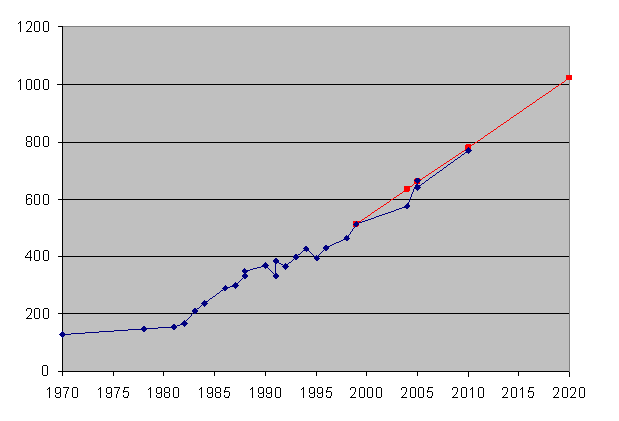
\includegraphics[scale=0.64, clip, viewport=-20 0 680 520]
                {figures/PrognoseRSAFaktorisierungSecorvo.png}
% Parameter von includegraphics: scale, x, y, dx, dy
% dx, dy spezifiziert die Ausdehnung, die man dem Bildes spendiert.
%      Ist dy zu klein, wird das Bild oben abgeschnitten
% x, y sagt, ab wo der Rahmen um das Bild gezeichnet wird.
%      Ist z.B. x=50, sind der linke Rahmenstrich und Teile des linken
%      Teiles des Bildes nicht zu sehen.
% scale dehnt Rahmenlinie und Bild aus -> Sitenrand wird bei 0.7 z.B. kleiner.
}
\caption{Vergleich der publizierten Faktorisierungserfolge (blau) mit der
prognostizierten Entwicklung (rot) [Quelle Fox 2001; letzte Erg�nzung 2011]}
\label{secorvo-factorisation-forecast}
\end{center}
\end{figure}




\clearpage  % Erzwingt, dass alle Floating Objekte (z.B. Grafiken VORHER
            % geschrieben werden ! (sonst wurde Kapitel 4.11.4 begonnen,
            % und die Secorvo-Grafik auf er Folgeseite UNTER die Fussnote
            % geschoben. Au�erdem wahrscheinlich auch Zeilenumbruch,
            % egal, ob nach der Garfik noch Platz ist.
% ++++++++++++++++++++++++++++++++++++++++++++++++++++++++++++++++++++++++++
\begin{ctsquote}
    Damit das M�gliche entsteht, muss immer wieder das Unm�gliche 
    versucht werden.
\caption[Hermann Hesse]{Hermann Hesse\footnotemark}
\end{ctsquote}
\addtocounter{footnote}{0}\footnotetext{%
    Hermann Hesse, deutsch-schweizerischer Schriftsteller und Nobelpreistr�ger, 
    02.07.1877$-$09.08.1962.}
% ++++++++++++++++++++++++++++++++++++++++++++++++++++++++++++++++++++++++++

\subsection{Status der Faktorisierung von konkreten gro�en Zahlen}
\label{nt:NoteFactorization}

Ausf�hrliche �bersichten �ber die Rekorde im Faktorisieren
zusammengesetzter Zahlen \index{Faktorisierung!Faktorisierungsrekorde}
mit unterschiedlichen Methoden finden sich auf den folgenden Webseiten:
\vspace{-10pt}
\begin{itemize}
\item[]
     \url{http://www.crypto-world.com} \\
     \url{http://www.tutorgig.com/ed/RSA\_number} ~~ The RSA Factoring Challenge \\
% footnote{%
% Diese Seite war Ende Mai 2005 nicht ganz auf dem aktuellen Stand: RSA-200 fehlte.}.
     \url{http://en.wikipedia.org/wiki/Integer_factorization_records}\\
     \url{http://en.wikipedia.org/wiki/RSA_Factoring_Challenge}

\end{itemize}

Der aktuelle Rekord (Stand Nov. 2012) mit der GNFS-Methode (General Number
Field Sieve) \index{General Number Field Sieve (GNFS)} zerlegte eine
allgemeine $232$-stellige Dezimalzahl in ihre beiden Primfaktoren.

\vskip +10pt
Die letzten Rekorde\footnote{%
Die  "`RSA-Zahlen"' sind gro�e semiprime Zahlen (d.h. Zahlen, die genau aus
2 Primfaktoren bestehen)\index{Zahlen!semiprime}\index{Primzahl!semiprime}.
Sie wurden von der Firma RSA Security generiert und ver�ffentlicht: Im
Wettbewerb "`RSA Factoring Challenge"' wurden die Primfaktoren dieser Zahlen gesucht.\\
Siehe \url{http://www.rsa.com/rsalabs/node.asp?id=2092}.

Die RSA-Laboratorien schreiben ihre Challenges schon seit Anfang der
90er-Jahre aus. In der ersten RSA-Factoring-Challenge wurden die Zahlen, von RSA-100 bis
RSA-500, gem�� der Anzahl ihrer Dezimalstellen benannt; die zweite
RSA-Factoring-Challenge benannte die Zahlen anhand der Anzahl ihrer
Bin�rstellen. Innerhalb des zweiten Wettbewerbs wurden Geldpreise f�r die
erfolgreiche Faktorisierung von RSA-576 bis RSA-2048 ausgelobt (RSA-576, RSA-640
etc. in 64-er Schritten --- Die Zahl RSA-617 bildet eine Ausnahme, da sie
vor der �nderung des Namensschemas erzeugt wurde).
Leider beendete RSA Inc. die Challenge vorzeitig und zog die Preise zur�ck.
Alle noch ungel�sten RSA-Challenges der RSA-Labs finden sich inzwischen auch
auf der Webseite des Krypto-Wettbewerbs \glqq MysteryTwister C3\grqq~
(\url{http://www.mysterytwisterc3.org}).
\index{MTC3}\index{Challenge}\index{Cipher-Challenge}\index{Krypto-Wettbewerb}

Die "`C-Zahlen"' stammen aus dem Cunningham-Projekt:
\url{http://www.cerias.purdue.edu/homes/ssw/cun/}.
Diese sind Faktoren gro�er Mersennezahlen, die eine ganz spezielle
Struktur haben. Dies macht es um Gr��enordnungen einfacher, sie zu
faktorisieren, als Moduli gleicher L�ngen, die man f�r RSA erstellt.
                               }
mit Faktorisierungsverfahren f�r zusammengesetzte Zahlen
sind in der folgenden Tabelle~\ref{factorizationrecords} aufgef�hrt:

\begin{table}[ht]
\begin{center}
\begin{tabular}{|c|ccc@{}c|}
\hline
   & {\bf Dezimalstellen} & {\bf Bin�rstellen} & {\bf Faktorisiert am} & {\bf Faktorisiert von} \\
\hline
	&&&& \\
	RSA-768 & 	232 & 768 & Dez 2010 & Thorsten Kleinjung et al. \\
	RSA-200 & 	200 & 663 & Mai 2005 & Jens Franke et al. \\
	RSA-640\footnotemark & 	193 & 640 & Nov 2005 & Jens Franke et al. \\
	RSA-576 & 	174 & 576 & Dez 2003 & Jens Franke et al. \\
	RSA-160 & 	160 & 530 & Apr 2003 & Jens Franke et al. \\
	RSA-155	&	155 & 512 & Aug 1999 & Herman te Riele et al. \\
	\dots & & & & \\
	C307 & 		307 & 1017 & Mai 2007 & Jens Franke et al. \\
	C176 & 		176 & 583 & Mai 2005 & Kazumaro Aoki et al. \\
	C158 & 		158 & 523 & Jan 2002 & Jens Franke et al. \\
\hline
\end{tabular}
\caption{Die derzeitigen Faktorisierungsrekorde (Stand Nov. 2012)}  % Eyecatcher
\label{factorizationrecords}
\end{center}
\end{table}
\footnotetext{%
Eine Arbeitsgruppe des BSI l�ste die mit 20.000 US-Dollar dotierte Challenge
RSA-640 mit Hilfe der GNFS-Methode. Die Forscher ben�tigten f�r die
Zerlegung der Zahl in ihre beiden 320 Bit langen Primfaktoren rund f�nf
Monate Rechenzeit.

Die Forscher um Prof. Jens Franke (von der Universit�t Bonn, dem BSI und dem
CWI) waren nicht auf die Geldpreise aus, sondern wollten die Grenzen der
Forschung ausdehnen. Dadurch werden Aussagen �ber notwendige Minimall�ngen
f�r sichere RSA-Moduli fundierter. 

Siehe \url{http://www.heise.de/newsticker/meldung/print/65957}
}

%be_2005: Erzwingen, dass die Abb. noch in diesem Kapitel !


Laufzeituntersuchungen zur Faktorisierung\index{Faktorisierung} mit den
Open-Source Software-Paketen Pari-GP, SageMath, CrypTool 1 und CrypTool 2
finden sich in "`Zeitexperimente zur Faktorisierung"'.\footnote{%
R.-H. Schulz und H. Witten: "`Zeitexperimente zur Faktorisierung. Ein Beitrag
zur Didaktik der Kryptographie"', in LogIn Heft Nr. 166/167 (2010) 113-120,\\
\url{http://bscw.schule.de/pub/bscw.cgi/d864899/Schulz_Witten_Zeit-Experimente.pdf}
}

\vskip +20pt
%\noindent
Im Folgenden werden die letzten Rekorde aus Tabelle~\ref{factorizationrecords}
etwas ausf�hrlicher erl�utert\footnote{%
Die beiden dabei benutzten Methoden GNFS und SNFS werden kurz z.B. auf
den ff. Webseiten dargestellt:
\index{General Number Field Sieve (GNFS)}
\index{Special Number Field Sieve (SNFS)}
\begin{itemize}
\item[]
      \url{http://en.wikipedia.org/wiki/Special_number_field_sieve} \\
      \url{http://en.wikipedia.org/wiki/General_number_field_sieve}
\end{itemize}
\vspace{-10pt}
}:


% --------------------------------------------------------------------------
%\vskip +20pt
\paragraph*{RSA-155} \label{RSA-155} \index{RSA-155} 
\mbox{} % f�r Zeilenumbruch, da er // allein nicht mag ! xxxxxxxxx

Am 22. August 1999 fanden niederl�ndische Forscher die L�sung dieser 
RSA-Challenge. Sie zerlegten eine $155$-stellige Zahl in ihre beiden $78$-stelligen
Primfaktoren (vergleiche Kapitel~\ref{chptSecurityParam}).
Mit der $512$ Bit-Zahl RSA-155 war eine {\em magische} Grenze erreicht.



% --------------------------------------------------------------------------
\vskip +20pt
\paragraph*{C158} \label{C158} \index{C158} 
\mbox{} % f�r Zeilenumbruch, da er \\ allein nicht mag ! xxxxxxxxx
\hypertarget{C158-chap3}{}

Am 18. Januar 2002 zerlegten Forscher der Universit�t Bonn\footnote{%
\url{http://www.uni-bonn.de/Aktuelles/Pressemitteilungen/pm02/pm035-02.html}
} 
mit der GNFS-Methode (General Number Field Sieve) \index{General Number
Field Sieve (GNFS)} eine $158$-stellige Dezimalzahl in ihre beiden Primfaktoren 
(diese haben 73 und 86 Dezimalstellen).

Dieser Rekord fand deutlich weniger Aufmerksamkeit in der Presse als die
L�sung von RSA-155.

Die Aufgabe der Bonner Wissenschaftler entsprang auch nicht einer Challenge,
sondern die Aufgabe war, die letzten Primfaktoren der Zahl $2^{953}+1$ 
zu finden (siehe~\glqq Wanted List\grqq~des Cunningham-Projekts\index{Cunningham-Projekt}%
\footnote{%
Cunningham-Projekt: \url{http://www.cerias.purdue.edu/homes/ssw/cun/}}). 

Die 6 kleineren, schon vorher gefundenen Primfaktoren dieser Zahl waren:
$$
\begin{array}{c}
        3, 1907, 425796183929, \\ 
        1624700279478894385598779655842584377, \\
        3802306738549441324432139091271828121 \quad{\rm und} \\ 
        128064886830166671444802576129115872060027.
\end{array}
$$
\begin{sloppypar}
Die drei kleinsten Faktoren k�nnen leicht\footnote{%
Z.B. mit CT1\index{CrypTool 1} �ber das Men� 
{\bf Einzelverfahren \textbackslash{} RSA-Kryptosystem \textbackslash{} 
Faktorisieren einer Zahl}. \\
In sinnvoller Zeit zerlegt CT1 Zahlen bis 250 Bit L�nge (Zahlen gr��er als
1024 Bit werden von CT1 nicht angenommen). CT2 kann auch Zahlen gr��er 250
Bit L�nge zerlegen.
}
bestimmt werden.
Die n�chsten drei Primfaktoren wurden von P.~Zimmerman%
\footnote{\url{http://www.loria.fr/zimmerma/ecmnet}}, 
T.~Grandlund%
\footnote{\url{http://www.swox.se/gmp/}}
und R. Harley in den Jahren 1999 und 2000 mit der Methode der Elliptischen
Kurven gefunden.
\end{sloppypar}

Als letzter Faktor blieb der sogenannte Teiler  "`C158"',
von dem man bis dahin wusste, dass er zusammengesetzt ist, aber man kannte
seine Primfaktoren nicht (die folgenden drei Zeilen sind eine einzige Zahl):
$$
\begin{array}{c}
39505874583265144526419767800614481996020776460304936 \\
45413937605157935562652945068360972784246821953509354 \\
4305870490251995655335710209799226484977949442955603
\end{array}
$$
Die Faktorisierung von C158 ergab die beiden 73- und 86-stelligen Primfaktoren:
$$
\begin{array}{c}
3388495837466721394368393204672181522815830368604993048084925840555281177
\end{array}
$$
und
$$
\begin{array}{c}
1165882340667125990314837655838327081813101 \\
2258146392600439520994131344334162924536139.
\end{array}
$$
Damit wurde die Zahl $2^{953}+1$ vollst�ndig in ihre 8 Primfaktoren zerlegt.

\noindent\begin{minipage}{\textwidth}
\vspace{3ex}
Verweise:
\vspace{-10pt}
\begin{itemize}
\item[]   \url{http://www.loria.fr/~zimmerma/records/gnfs158}\\
          \url{http://www.crypto-world.com/FactorRecords.html}\\
          \url{http://www.crypto-world.com/announcements/c158.txt}
\end{itemize}
\end{minipage}
\vspace{24pt}



% --------------------------------------------------------------------------
\vskip +20pt
\paragraph*{RSA-160} \label{RSA-160} \index{RSA-160}\mbox{}
\hypertarget{RSA-160-chap3}{}

Am 1. April 2003 zerlegten Forscher der Universit�t Bonn\footnote{%
          \url{http://www.loria.fr/~zimmerma/records/rsa160} \\
          \url{http://www.loria.fr/~zimmerma/records/factor.html} \\
          \url{http://www.crypto-world.com/FactorWorld.html}
} 
mit der GNFS-Methode (General Number Field Sieve) \index{General Number
Field Sieve (GNFS)} eine $160$-stellige Zahl in ihre beiden Primfaktoren 
(diese haben jeweils 80 Dezimalstellen).

Die Berechnungen dazu fanden auch im Bundesamt f�r Sicherheit in der 
Informationstechnik (BSI) in Bonn statt.\footnote{%
Das BSI \index{BSI} erstellt jedes Jahr ein Papier �ber die Eignung von
Kryptoalgorithmen, mit denen Signaturen erzeugt werden k�nnen,         
die den Vorgaben des deutschen Signaturgesetzes gen�gen.
Bei dieser Erstellung werden Experten aus Wirtschaft und Wissenschaft
beteiligt. Um die Eignung von Signaturverfahren zu beurteilen, deren
Schwierigkeit auf dem Faktorisierungsproblem beruht,
kooperiert das BSI auch mit Forschern der Universit�t Bonn.
Weitere Informationen zu Kryptoalgorithmen finden Sie auf den BSI-Internetseiten unter:
   \url{http://www.bsi.bund.de/esig/basics/techbas/krypto/index.htm}
}

Die 160-stellige Dezimalzahl stammt von der alten Challenge-Liste von RSADSI.
Diese wurde nach der Faktorisierung von RSA-155 (RSA512) zur�ckgezogen.
Die Primfaktoren von RSA-160 waren aber nicht bekannt.
Deshalb ist dieser Rekord von Prof.\ Frankes Team immer noch die L�sung 
einer alten Challenge, f�r die es aber von RSADSI kein Geld gibt.

Die zusammengesetzte Zahl "`RSA-160"' lautet (die folgenden drei Zeilen 
sind eine einzige Zahl):
$$
\begin{array}{c}
215274110271888970189601520131282542925777358884567598017049 \\
767677813314521885913567301105977349105960249790711158521430 \\
2079314665202840140619946994927570407753
\end{array}
$$
Die Faktorisierung von RSA-160 ergab die beiden Primfaktoren:
$$
\begin{array}{c}
p = 45427892858481394071686190649738831 \\         
    656137145778469793250959984709250004157335359
\end{array}
$$
und
$$
\begin{array}{c}
q = 47388090603832016196633832303788951 \\
    973268922921040957944741354648812028493909367
\end{array}
$$

Die Berechnungen erfolgten zwischen Dezember 2002 und April 2003.
\vspace{24pt}



% ammmmmmmmmmma
% 
% RSA-576 faktorisiert 
% Am 27.04.2004 ging die Nachricht durch
% die Ticker, dass die 576-bit-Challenge der
% Firma RSA gel�st sei. Tats�chlich wurde
% die 174 Dezimalstellen lange Zahl bereits
% am 03.12.2003 zerlegt. Die Faktorisierung
% gelang einem Team der Universit�t Bonn
% um Professor Franke mit Unterst�tzung
% durch das Institut f�r Experimentelle Mathematik
% in Essen und das BSI. Die verteilte
% Berechung erfolge auf einem Linux-
% Cluster mit 144 PCs (400 MHz, Pentium II)
% und verwendete den General Number Field
% Sieve-Algorithmus ? mit einem Aufwand
% von umgerechnet 13.200 MIPS-Jahren.
% Interessant dabei: Dieser Faktorisierungserfolg
% best�tigt die Prognose, die Secorvo
% vor drei Jahren auf der Basis der Faktorisierungserfolge
% der vergangenen 30 Jahre
% gestellt hat (siehe Bild), und die weit weniger
% dramatisch ausfiel als viele Expertenwarnungen
% und die Erwartung des BSI.
% Danach w�re 2004 erstmals die Faktorisierung
% einer 630 bit langen Zahl zu erwarten
% gewesen ? was nun eher unwahrscheinlich
% erscheint. Selbst die fr�hestens f�r das
% Jahr 2020 vorausgesagte Faktorisierung
% eines 1024 bit langen RSA-Schl�ssels
% k�nnte sich daher noch als zu pessimistische
% Bef�rchtung erweisen ? allen Warnern
% zum Trotz, die seit Jahren Schl�ssell
% �ngen von 2048 bit und mehr empfehlen
% oder gar das baldige Ende von RSA prophezeihen.
% 
% ammmmmmmmmmmz




% --------------------------------------------------------------------------
\vskip +20pt
\hypertarget{RSA-200-chap3}{}
\paragraph*{RSA-200} \label{RSA-200} \index{RSA-200}\mbox{}
\nopagebreak

Am 9. Mai 2005 meldete die Forschergruppe von Prof. Jens Franke der Universit�t Bonn\footnote{%
   \url{http://www.loria.fr/~zimmerma/records/rsa200}}, dass sie
gemeinsam mit Kollegen des Amsterdam Centrum voor Wiskunde en Informatica
einen neuen Weltrekord im Faktorisieren aufstellten. 

Sie zerlegten mit der GNFS-Methode (General Number Field Sieve) \index{General Number
Field Sieve (GNFS)} eine $200$-stellige Zahl in ihre beiden Primfaktoren 
(diese haben jeweils 100 Dezimalstellen).

Die zusammengesetzte Zahl "`RSA-200"' lautet (die folgenden drei Zeilen 
sind eine einzige Zahl):
$$
\begin{array}{c}
2799783391122132787082946763872260162107044678695542853756000992932 \\
6128400107609345671052955360856061822351910951365788637105954482006 \\
576775098580557613579098734950144178863178946295187237869221823983
\end{array}
$$
Die Faktorisierung von RSA-200 ergab die beiden Primfaktoren:
$$
\begin{array}{c}
p = 35324619344027701212726049781984643686711974001976 \\
    25023649303468776121253679423200058547956528088349
\end{array}
$$
und
$$
\begin{array}{c}
q = 79258699544783330333470858414800596877379758573642 \\
    19960734330341455767872818152135381409304740185467
\end{array}
$$

Die Berechnungen erfolgten zwischen Dezember 2003 und Mai 2005.
Die Faktorisierung durch die Gruppe um Bahr, B�hm, Franke, Kleinjung, 
Montgomery und te Riele hatte also knapp 17 Monate gedauert.
Der Rechenaufwand lag bei umgerechnet etwa 120.000 MIPS-Jahren\footnote{%
Ein MIPS-Jahr (MY) ist die Anzahl von Operationen, die eine Maschine, 
welche eine Million Integeroperationen pro Sekunde (MIPS)
ausf�hrt, in einem Jahr bew�ltigt. Zur Illustration: ein INTEL 
Pentium 100 Prozessor hat etwa 50 MIPS.
F�r die Zerlegung eines 2048-Bit-Moduls br�uchte man ca. {$8,5 \cdot 
10^{40}$ MY}.}.
\vspace{24pt}




% --------------------------------------------------------------------------
\vskip +20pt
\hypertarget{RSA-768-chap3}{}
\paragraph*{RSA-768} \label{RSA-768} \index{RSA-768}\mbox{}
\nopagebreak

Am 12. Dezember 2009 meldete die Forschergruppe um Prof. Thorsten
Kleinjung\footnote{%
   \url{http://eprint.iacr.org/2010/006.pdf} \cite{nt:Kleinjung2010}
          }, dass sie
eine $232$-stellige Zahl in ihre beiden Primfaktoren zerlegten 
(diese haben jeweils 116 Dezimalstellen).
Sie benutzten dazu die GNFS-Methode (General Number Field Sieve)
\index{General Number Field Sieve (GNFS)} in einer Art, dass vor dem
Matrix-Schritt auf mehreren hundert Rechnern "`Oversieving"' betrieben wurde. 

Die zusammengesetzte Zahl "`RSA-768"' lautet (die folgenden drei Zeilen 
sind eine einzige Zahl):
$$
\begin{array}{c}
123018668453011775513049495838496272077285356959533479219732245215172640050726\\
365751874520219978646938995647494277406384592519255732630345373154826850791702\\
6122142913461670429214311602221240479274737794080665351419597459856902143413
\end{array}
$$
Die Faktorisierung von RSA-768 ergab die beiden Primfaktoren (je 384 bit):
$$
\begin{array}{c}
p = 3347807169895689878604416984821269081770479498371376856891\\
    2431388982883793878002287614711652531743087737814467999489
\end{array}
$$
und
$$
\begin{array}{c}
q = 3674604366679959042824463379962795263227915816434308764267\\
    6032283815739666511279233373417143396810270092798736308917
\end{array}
$$

Die Berechnungen dauerten 2 1/2 Jahre.\footnote{%
Dies war ein "`academic effort"' -- Organisationen mit besserer Ressourcen-Ausstattung
k�nnten es deutlich schneller durchf�hren.}
\vspace{24pt}





% --------------------------------------------------------------------------
\vskip +20pt
\paragraph*{C307 / M1039} \label{C307} \index{C307} \index{M1039} 
\mbox{} % f�r Zeilenumbruch, da er \\ allein nicht mag ! xxxxxxxxx
\hypertarget{C307-chap3}{}

Im Mai 2007 meldeten Prof. Franke, Prof. Kleinjung (von der Universit�t Bonn),
das japanische Telekommunikationsunternehmen NTT und Prof. Arjen Lenstra von
der Polytechnischen Hochschule in Lausanne, dass sie mit der SNFS-Methode
(Special Number Field Sieve) \index{Special Number Field Sieve (SNFS)}
innerhalb von 11 Monaten eine $307$-stellige Dezimalzahl in ihre beiden
Primfaktoren zerlegten (diese haben 80 und 227 Dezimalstellen).

Die Aufgabe der Wissenschaftler entsprang nicht einer Challenge, sondern
die Aufgabe war, die letzten Primfaktoren der Mersenne-Zahl $2^{1039}+1$ 
zu finden (siehe~ \glqq Wanted List\grqq~ des Cunningham-Projekts\index{Cunningham-Projekt}%
\footnote{%
Cunningham-Projekt: \url{http://www.cerias.purdue.edu/homes/ssw/cun/}\\
Cunningham-Tabelle: \url{http://homes.cerias.purdue.edu/~ssw/cun/pmain1206}\\
Die Zahlen in der Cunningham-Tabelle werden folgenderma�en geschrieben:\\
\glqq (2,n)-\grqq~ bedeutet $2^{n}-1$;~~~
\glqq (2,n)+\grqq~ bedeutet $2^{n}+1$.\\
Um die Gr��enordnung einer Zerlegung anzudeuten schreibt man $p<n>$ oder $c<n>$,
wobei \glqq n\grqq~ die Anzahl der Dezimalstellen ist und \glqq p\grqq~ und \glqq c\grqq~
bedeuten, dass die Zahl eine Primzahl oder eine zusammengesetzte Zahl ist.\\
$2^{1039}-1 = p7 * c307 = p7 * p80 * p227$ \\
Genauer erkl�rt wird dies auf der Seite zum Cunningham-Projekt folgenderma�en:\\
\glqq 2,651+ means $2^{651} + 1$ and the size (c209 means 209 decimal digits)
of the
number which was factored.  Then come the new factor(s), the discoverer and
the method used.  Recently, only the multiple polynomial quadratic sieve
(ppmpqs), the elliptic curve method (ecm) and the number field sieve (nfs)
have been used.  `hmpqs' stands for hypercube multiple polynomial quadratic
sieve.  Under `new factors', `p90' means a 90-digit prime and `c201' is a
201-digit composite number.\grqq. 
}).\\


Die Zahl $2^{1039}-1$ besteht aus 3 Primfaktoren: Der kleinste Faktor
$p7 = 5080711$ war schon l�nger bekannt.\footnote{%
Er kann mit CT1\index{CrypTool 1} �ber das Men� 
{\bf Einzelverfahren \textbackslash{} RSA-Kryptosystem \textbackslash{} 
Faktorisieren einer Zahl} gefunden werden --- mit den Algorithmen von Brent,
Williams oder Lenstra, mit denen man gut \glqq relativ\grqq~ kleine Faktoren
abspalten kann.}

Zur vollst�ndigen Faktorisierung musste der zweite Faktor (Koteiler) "`C307"'
zerlegt werden: Bis dahin wusste man nur, dass er zusammengesetzt ist, aber man
kannte weder die Anzahl seiner Primfaktoren, noch die Primfaktoren selbst.
Die folgenden f�nf Zeilen sind eine einzige Zahl:
$$
\begin{array}{c}
C307 =1159420574072573064369807148876894640753899791702017724986868353538\\
8224838599667566080006095408005179472053993261230204874402860435302\\
8619141014409345351233471273967988850226307575280937916602855510550\\
0425810771176177610094137970787973806187008437777186828680889844712\\
822002935201806074755451541370711023817
\end{array}
$$
Die Faktorisierung von C307 ergab die beiden 80- und 227-stelligen Primfaktoren:
$$
\begin{array}{c}
p80 = 558536666199362912607492046583159449686465270184\\
      88637648010052346319853288374753
\end{array}
$$
und
$$
\begin{array}{c}
p227 = 207581819464423827645704813703594695162939708007395209881208\\
       387037927290903246793823431438841448348825340533447691122230\\
       281583276965253760914101891052419938993341097116243589620659\\
       72167481161749004803659735573409253205425523689
.
\end{array}
$$
Damit wurde die Zahl $2^{1039}-1$ vollst�ndig in ihre 3 Primfaktoren zerlegt.

\noindent\begin{minipage}{\textwidth}
\vspace{3ex}
Verweise:
\vspace{-10pt}
\begin{itemize}
\item[]   \url{http://www.loria.fr/~zimmerma/records/21039-}\\
          \url{http://www.crypto-world.com/announcements/m1039.txt}\\
          \url{http://www.crypto-world.com/FactorAnnouncements.html}\\
          \url{http://www1.uni-bonn.de/pressDB/jsp/pressemitteilungsdetails.jsp?detailjahr=2007&detail=160}
\end{itemize}
\end{minipage}






% --------------------------------------------------------------------------
\vskip +50pt
\paragraph*{Gr��enordnung faktorisierter Zahlen im Vergleich zu auf Primalit�t
getesteter Zahlen}
\mbox{}

Wie man sieht, sind die gr��ten (aus 2 Primfaktoren) zusammengesetzten
Zahlen, die man faktorisieren kann, deutlich kleiner als die Zahlen mit
einer speziellen Struktur, f�r die Primzahltests\index{Primzahltest} in
der Lage sind, Aussagen �ber ihre Primalit�t zu treffen (siehe Kapitel 
\ref{search_for_very_big_primes},~\ref{primality_tests} und
\ref{spezialzahlentypen}).


% be_2005_UPDATEN_if-new-mersenne-prime-appears   % Eyecatcher_neue-Mersenne
L�nge der derzeitigen Weltrekorde in Dezimaldarstellung:

$$  ~~~~~~~~~[RSA{-}768{-}Zahl] ~~\longleftrightarrow{}~~[49.~bekannte~Mersenne~Primzahl] $$
$$ 232 ~~ \longleftrightarrow{} ~~ 22.338.618 ~~~~~$$
$$ [vgl.~Tab.~\ref{factorizationrecords}] ~~\longleftrightarrow{}~~ [vgl.~Tab.~\ref{L_n_Largest_Known-Primes}] ~~~~~~~~~~~~~~~~$$

%be_2005 - erzwungenes Blank und $$ um Pfeilzeichen, sonst setzt er Blanks an 
%          die falschen Stellen.
%        - Wenn man hier \~ statt nur ~ (au�erhalb der $$) schreibt, kommen
%          nachher Fussnoten mit 
%          {\bf Einzelverfahren \textbackslash{} Protokolle}
%          nur noch mit kaputten Schriftzeichen raus !



% --------------------------------------------------------------------------
\vskip +60pt
\subsection[Weitere aktuelle Forschungsergebnisse zu Primzahlen und Faktorisierung]
           {Weitere aktuelle Forschungsergebnisse zu Primzahlen und Faktorisie"-rung}
\label{FactorisationResearch}
Primzahlen sind Teil vieler hochaktueller Forschungsgebiete der Zahlentheorie. 
Die Fortschritte bei der Faktorisierung sind gr��er als noch vor 5 Jahren
gesch�tzt -- sie gehen nicht nur auf das Konto schnellerer Rechner, 
sondern sie sind auch in neuen mathematischen Erkenntnissen begr�ndet.

Die Sicherheit des RSA-Algorithmus basiert auf der empirischen Beobachtung, dass die Faktorisierung gro�er ganzer 
Zahlen ein schwieriges Problem ist. Besteht wie beim RSA-Algorithmus der zugrunde liegende Modul $n$ aus dem Produkt 
zweier gro�er Primzahlen $p, q$ (typische L�ngen: $p, q$  $500-600$ bit, $n$ $1024$ bit), so l�sst sich 
$n=pq$ aus $p$ und $q$ leicht bestimmen, jedoch ist es mit den bisher bekannten Faktorisierungsalgorithmen nicht
m�glich, $p, q$ aus $n$ zu gewinnen. Nur mit Kenntnis von $p$ und $q$ l�sst sich jedoch der private aus dem 
�ffentlichen Schl�ssel ermitteln.

Die Entdeckung eines Algorithmus zur effizienten Faktorisierung von Produkten $n=pq$ gro�er Primzahlen w�rde daher 
den RSA-Algorithmus wesentlich beeintr�chtigen. Je nach Effizienz der Faktorisierung im Vergleich zur Erzeugung von 
$p, q, n$ m�sste der verwendete Modul $n$ (z.Zt. 1024 bit) erheblich vergr��ert oder --- im Extremfall --- auf den 
Einsatz des RSA ganz verzichtet werden.


% --------------------------------------------------------------------------
\vskip +20pt
%\paragraph*
\subsubsection{Das Papier von Bernstein und seine Auswirkungen auf die Sicherheit
               des RSA-Algorithmus}
\label{RSABernstein} \index{Faktorisierung!Faktorisierungsproblem}
%\mbox{} % f�r Zeilenumbruch, da er \\ allein nicht mag ! 
        % Braucht die Leerzeile danach auch noch !! bebebe ?
Die im November 2001 ver�ffentlichte Arbeit \glqq Circuits for integer
factorization: a proposal\grqq~(siehe \url{http://cr.yp.to/djb.html})
von D.J. Bernstein \cite{nt:Bernstein2001} behandelt das Problem der 
Faktorisierung gro�er Zahlen.
Die Kernaussage des Papers besteht darin, dass es m�glich ist, die
Implementierung des General Number Field Sieve-Algorithmus (GNFS)
\index{General Number Field Sieve (GNFS)} so zu
verbessern, dass mit gleichem Aufwand wie bisher Zahlen mit 3-mal
gr��erer Stellenzahl (Bit-L�nge) faktorisiert werden k�nnen.

Wesentlich bei der Interpretation des Resultats ist die Definition des
Aufwandes: Als Auf"-wand wird das Produkt von ben�tigter Rechenzeit und
Kosten der Maschine (insbesondere des verwendeten Speicherplatzes)
angesetzt. Zentral f�r das Ergebnis des Papiers ist die Beobachtung, dass
ein wesentlicher Teil der Faktorisierung auf Sortierung zur�ckgef�hrt
werden kann und mit dem Schimmlerschen Sortierschema ein Algorithmus zur
Verf�gung steht, der sich besonders gut f�r den Einsatz von
Parallelrechnern eignet. Am Ende des Abschnittes 3 gibt Bernstein konkret
an, dass die Verwendung von $m^2$ Parallelrechnern mit jeweils gleicher
Menge an Speicherplatz mit Kosten in der Gr��enordnung von $m^2$
einhergeht --- genau so wie ein einzelner Rechner mit $m^2$ Speicherzellen.
Der Parallelrechner bew�ltigt die Sortierung von $m^2$ Zahlen jedoch
(unter Verwendung der o.~g.\ Sortierverfahrens) in Zeit proportional zu m,
wohingegen der Einprozessorrechner Zeit proportional $m^2$ ben�tigt.
Verringert man daher den verwendeten Speicherplatz und erh�ht --- bei
insgesamt gleich bleibenden Kosten --- die Anzahl der Prozessoren
entsprechend, verringert sich die ben�tigte Zeit um die Gr��enordnung
$1/m$. In Abschnitt 5 wird ferner angef�hrt, dass der massive Einsatz der
parallelisierten Elliptic Curve-Methode von Lenstra die Kosten der
Faktorisierung ebenfalls um eine Gr��enordnung verringert (ein
Suchalgorithmus hat dann quadratische statt kubische Kosten).  Alle
Ergebnisse von Bernstein gelten nur asymptotisch f�r gro�e Zahlen $n$.
Leider liegen keine Absch�tzungen �ber den Fehlerterm, d.h.  die
Abweichung der tats�chlichen Zeit von dem asymptotischen Wert, vor --- ein
Mangel, den auch Bernstein in seinem Papier erw�hnt. Daher kann zur Zeit
keine Aussage getroffen werden, ob die Kosten (im Sinne der Bernsteinschen
Definition) bei der Faktorisierung z.~Zt.\ verwendeter RSA-Zahlen
(1024$-$2048 bit) bereits signifikant sinken w�rden.

Zusammenfassend l�sst sich sagen, dass der Ansatz von Bernstein durchaus 
innovativ ist. Da die Verbesserung der 
Rechenzeit unter gleichbleibenden Kosten durch einen massiven Einsatz von 
Parallelrechnern erkauft wird, stellt sich die 
Frage nach der praktischen Relevanz. Auch wenn formal der Einsatz von einem 
Rechner �ber 1 sec  und  1.000.000 Rechnern 
f�r je 1/1.000.000 sec dieselben Kosten erzeugen mag, ist die 
Parallelschaltung von 1.000.000 Rechnern praktisch nicht 
(oder nur unter immensen Fixkosten, insbesondere f�r die Vernetzung der
Prozessoren) zu realisieren. Solche Fixkosten 
werden aber nicht in Ansatz gebracht.
Die Verwendung verteilter Ans�tze (distributed computing) �ber ein 
gro�es Netzwerk k�nnte einen Ausweg bieten. Auch hier m�ssten  
Zeiten und Kosten f�r Daten�bertragung einkalkuliert werden.

Solange noch keine (kosteng�nstige) Hardware oder verteilte Ans�tze 
entwickelt wurden, die auf 
dem Bernsteinschen Prinzip basieren, besteht noch keine akute Gef�hrdung
des RSA. Es bleibt zu kl�ren, ab welchen 
Gr��enordnungen von n die Asymptotik greift. 

Arjen Lenstra, Adi Shamir et.~al.\ haben das Bernstein-Paper analysiert 
\cite{nt:Lenstra2002}.
Als Ergebnis kommen Sie zu einer Bitl�ngen-Verbesserung der 
Faktorisierung um den Faktor 1.17 
(anstatt Faktor 3 wie von Bernstein erwartet).

Die Zusammenfassung ihres Papers \glqq Analysis of Bernstein's Factorization 
Circuit\grqq~lautet:

\glqq ... Bernstein proposed a circuit-based implementation of
the matrix step of the number field sieve factorization algorithm. We
show that under the non-standard cost function used in [1], these circuits
indeed offer an asymptotic improvement over other methods but
to a lesser degree than previously claimed: for a given cost, the new
method can factor integers that are 1.17 times larger (rather than 3.01).
We also propose an improved circuit design based on a new mesh routing
algorithm, and show that for factorization of 1024-bit integers the
matrix step can, under an optimistic assumption about the matrix size,
be completed within a day by a device that costs a few thousand dollars.
We conclude that from a practical standpoint, the security of RSA relies
exclusively on the hardness of the relation collection step of the number
field sieve.\grqq

Auch RSA Security\footnote{\url{http://www.rsasecurity.com/}} kommt in ihrer
Analyse der Bernstein-Arbeit \cite{nt:RSA Security 2002} vom 8. April 2002
erwartungsgem�� zu dem Ergebnis, dass RSA weiterhin als ungebrochen betrachtet
werden kann.

Die Diskussion ist weiterhin im Gang.

Zum Zeitpunkt der Erstellung dieses Absatzes (Juni 2002) war nichts
dar�ber bekannt, inwieweit die im Bernstein-Papier vorgeschlagenen
theoretischen Ans�tze realisiert wurden oder wieweit die Finanzierung
seines Forschungsprojektes ist.

\noindent\begin{minipage}{\textwidth}
\vspace{3ex}
Verweise:
\vspace{-10pt}
\begin{itemize}
  \item[] \url{http://cr.yp.to/djb.html}\\
          \url{http://www.counterpane.com/crypto-gram-0203.html\#6} \\
          \url{http://www.math.uic.edu}
\end{itemize}
\end{minipage}



% --------------------------------------------------------------------------
\vskip +20pt
%\paragraph*
\subsubsection{Das TWIRL-Device} \label{TWIRLDevice} \index{TWIRL-Device}
%\mbox{} % f�r Zeilenumbruch, da er // allein nicht mag ! xxxxxxxxx

Im Januar 2003 ver�ffentlichten Adi Shamir und Eran Tromer vom Weizmann
Institute of Science den vorl�ufigen Draft {\em \glqq Factoring Large Numbers
with the TWIRL Device\grqq}, in dem deutliche Bedenken gegen RSA-Schl�ssell�ngen
unter 1024 begr�ndet werden \cite{nt:Shamir2003}.

Das Abstract fasst ihre Ergebnisse folgenderma�en zusammen: \glqq The security of the RSA cryptosystem depends on the difficulty of factoring large integers. The best current factoring algorithm is the Number Field Sieve (NFS), and its most difficult part is the sieving step. In 1999 a large distributed computation involving thousands of workstations working for many months managed to factor a 512-bit RSA key, but 1024-bit keys were believed to be safe for the next 15-20 years. In this paper we describe a new hardware implementation of the NFS sieving step ... which is 3-4 orders of magnitude more cost effective than the best previously published designs ... . Based on a detailed analysis of all the critical components (but without an actual implementation), we believe that the NFS sieving step for 1024-bit RSA keys can be completed in less than a year by a \$10M device, and that the NFS sieving step for 512-bit RSA keys can be completed in less than ten minutes by a \$10K device. Coupled with recent results about the difficulty of the NFS matrix step ... this raises some concerns about the security of these key sizes.\grqq

Eine ausf�hrliche Fassung findet sich auch in dem Artikel der beiden Autoren
in den RSA Laboratories CryptoBytes \cite{nt:Shamir2003a}.

Eine sehr gute Erl�uterung, wie der Angriff mit dem Generalized Number Field
Sieve (GNFS) \index{General Number Field Sieve (GNFS)} funktioniert und
welche Fortschritte sich ergaben, findet sich
in dem 3-seitigen Artikel in der DuD-Ausgabe Juni/2003 \cite{nt:Weis2003}.
Beim GNFS k�nnen 2 grundlegende Schritte unterschieden werden: 
der Siebungsschritt (Relationen sammeln) und die Matrix-Reduktion.
Auch wenn der Siebungsschritt hochgradig parallelisierbar ist, so dominiert
er doch den Gesamtrechenaufwand. Bisher haben Shamir und Tromer noch kein 
TWIRL-Device gebaut, jedoch ist der daf�r ge"-sch�tzte Aufwand von 10 bis
50 Millionen Euro, um eine 1024-Bit Zahl in einem Jahr zu faktorisieren
f�r Geheimdienste oder gro�e kriminelle Organisationen keineswegs prohibitiv,
denn die \glqq Kosten f�r einen einzigen Spionagesatelliten sch�tzt man
z.B. auf mehrere Milliarden USD\grqq. Die Autoren empfehlen deshalb konkret,
m�glichst rasch sensible, bisher benutzte RSA-, Diffie-Hellman- oder 
ElGamal-Schl�ssel von bis zu 1024 Bit zu wechseln und Schl�ssel von 
mindestens 2048 Bit L�nge einzusetzen.
Auch f�r die geplante TCPA/Palladium-Hardware \index{Palladium} werden
2048-Bit RSA-Schl�ssel verwendet!

Damit erscheinen die aktuellen Empfehlungen des BSI, auf l�ngere 
RSA-Schl�ssell�ngen umzustellen, mehr als gerechtfertigt.



% --------------------------------------------------------------------------
\vskip +20pt
%\paragraph*{``Primes in P'': Testen auf Primalit�t ist polynominal}
\subsubsection{\glqq Primes in P\grqq: Testen auf Primalit�t ist polynominal}
\label{PrimesinP} \index{Primzahltest} 
%\mbox{} % f�r Zeilenumbruch, da er // allein nicht mag ! xxxxxxxxx

Im August 2002 ver�ffentlichten die drei indischen Forscher M. Agrawal, 
N. Kayal und N. Saxena ihr Paper {\em \glqq PRIMES in P\grqq}  %{\em ``PRIMES in P''} 
�ber einen neuen Primzahltest-Algorithmus, genannt AKS\index{AKS} \cite{nt:Agrawal2002}.
Sie entdeckten einen polynominalen\index{Polynom} deterministischen Algorithmus, um zu entscheiden, ob eine gegebene Zahl prim ist oder nicht.

Die Bedeutung dieser Entdeckung liegt darin, dass sie Zahlentheoretiker mit neuen Einsichten und M�glichkeiten f�r die weitere Forschung versorgt. Viele Menschen haben im Lauf der Jahrhunderte nach einem polynominalen Primzahltest gesucht, so dass dieses Ergebnis einen theoretischen Durchbruch darstellt. Es zeigt sich immer wieder, dass aus schon lange bekannten Fakten neue Ergebnisse generiert werden k�nnen.

Aber selbst die Autoren merken an, dass andere bekannte Algorithmen (z.B. ECPP) schneller sein k�nnen. Der neue Algorithmus funktioniert f�r alle positiven ganzen Zahlen. Dagegen verwendet das GIMPS-Projekt den Lucas-Lehmer-Primzahltest, der besondere Eigenschaften der Mersennezahlen ausnutzt. Dadurch ist der Lucas-Lehmer-Test viel schneller und erlaubt, Zahlen mit Millionen von Stellen zu testen, w�hrend generische Algorithmen auf Zahlen mit einigen tausend Stellen beschr�nkt sind. Nachteil der bisherigen schnellen Verfahren ist, dass sie probabilistisch sind, also ihr Ergebnis h�chstwahrscheinlich, aber nicht ganz sicher ist.

\enlargethispage{20pt}
\noindent Aktuelle Forschungsergebnisse dazu finden sich z.B. auf: 
\vspace{-10pt}
\begin{itemize}
  \item[] \url{http://www.mersenne.org/} \\
          \url{http://fatphil.org/maths/AKS/} Originaltext in Englisch\\
          \href{http://ls2-www.cs.uni-dortmund.de/lehre/winter200203/kt/material/primes.ps}{\tt http://ls2-www.cs.uni-dortmund.de/lehre/winter200203/kt/material/primes.ps} \\% \url... created overfull \hbox
           \hspace*{2em}\hspace*{2em}Gute Erl�uterung in Deutsch von Thomas Hofmeister.
\end{itemize}
\vskip +10 pt



% --------------------------------------------------------------------------
\vskip +20pt
\subsubsection{\glqq Shared Primes\grqq: Module mit gleichen Primfaktoren}
\label{nt_Shared-Primes} \index{Primzahl!Shared} 
%~\ref{nt_Shared-Primes}, S.~\pageref{nt_Shared-Primes}

Der RSA-Algorithmus basiert auf der angenommenen Schwierigkeit, gro�e semi-prime
nat�rliche Zahlen (Module) zu faktorisieren (Faktorisierungsproblem).
Wie Lenstra et al \cite{nt:Lenstra2012} beschrieben, ist es aber m�glich, aus
einer gegebenen Menge von Modulen einige zu faktorisieren, sofern sie
gemeinsame Primfaktoren (shared primes) aufweisen. In diesem Fall kann das 
Faktorisierungsproblem umgangen werden, indem man die -- relativ einfach zu
berechnenden -- gr��ten gemeinsamen Teiler (ggT) bestimmt. Andererseits ist es
keine triviale Aufgabe, alle Shared Primes (gemeinsame Primfaktoren) effizient
zu bestimmen und die zugeh�rigen Module zu faktorisieren, wenn die gegebene
Menge von Moduln sehr gro� ist (mehrere Millionen).

Die ggTs lassen sich nur nutzen, wenn die RSA-Schl�ssel nicht zuf�llig genug
erzeugt wurden. Zieht man die Wichtigkeit starker kryptographischer Schl�ssel
in Betracht, sollte man verifizieren, dass alle Schl�ssel (wirklich)
zuf�llig erzeugt wurden \cite{nt:Esslinger2012}. 

Als Lenstra et al ihr Paper \cite{nt:Lenstra2012} im Februar 2012 
ver�ffentlichten, ver�ffentlichten sie nicht den zugeh�rigen Source-Code.
Kurz danach wurde der Source-Code eines �hnlichen Programms auf der
CrypTool-Website\footnote{%
\url{http://www.cryptool.org/en/ctp-dokumentation-en/361-ctp-paper-rsa-moduli}
%\url{http://www.cryptool.org/de/ctp-dokumentation-de/361-ctp-paper-rsa-moduli}
}
in Python und C++ ver�ffentlicht, und noch etwas sp�ter auf der Seite, die von
\cite{nt:Heninger2012}\footnote{\url{https://www.factorable.net/}
} benutzt wurde.
Der schnellste bisher bekannte Code ist von \cite{nt:Heninger2012}.

Diese Programme finden alle eventuell existierenden gemeinsamen Primfaktoren aus
einer gegebenen Menge von Modulen, auch wenn diese Menge Millionen von
Modulen enth�lt. Mit diesen Programmen k�nnen dann System-Administratoren ihre
eigenen RSA-Schl�ssel testen.

Der einfachste Ansatz, alle Primfaktoren zu finden (indem man jeden Modul mit
jedem anderen vergleicht), hat eine Komplexit�t, die quadratisch mit der Anzahl
der Modulen w�chst.

Eine sehr effiziente Methode, die B�ume zum Vergleich aller ggT-Paare benutzt,
basiert auf einer Publikation von Dan Bernstein aus 2005 \cite{nt:Bernstein2005}. Bernstein benutzt eine Vorberechnung, in der das Produkt aller Module erzeugt wird. Das ist ein weiteres Beispiel daf�r, wie hilfreich Vorberechnungen sein k�nnen, um kryptographische Systeme zu brechen (ein anderes ber�hmtes Beispiel sind die Rainbow-Tabellen, um die Ursprungswerte von Hashwertes zu finden \cite{nt:Oechslin2003}).


Das folgende SageMath-Beispiel zeigt die sehr unterschiedlichen Laufzeiten f�r die Berechnung eines ggT und einer Faktorisierung. In dem Abschnitt nach diesem Beispiel wird der Kern der Methode erkl�rt, der in \cite{nt:Heninger2012} benutzt wird: Die Benutzung von zwei B�umen beschleunigt die Berechnung deutlich.

Das SageMath-Beispiel~\ref{nt_sagesample_Compare-Runtime-gcd-factoring} zeigt, dass die folgenden Operationen sehr schnell sind: Multiplikation von Faktoren, Dividieren eines Moduls durch einen bekannten Faktor und Berechnen des ggT. Im Gegensatz dazu steigt die Rechendauer zur Faktorisierung von l�ngeren Moduli stark an. Selbst die relativ kleinen Module in diesem Beispiel zeigen das: Der kleinere Modul (69 Dezimalstellen, 228 bit) brauchte 76 Sekunden, w�hrend der gr��ere (72 Dezimalstellen, 239 bit) schon fast 217 Sekunden ben�tigte.

Hinzu kommt, dass die Operationen Multiplikation, Division und ggT gro�e Laufzeit-Unter"-schiede aufweisen, wenn die Operanden von sehr unterschiedlicher Gr��e sind.

% Just to show the origin of the used primes
% sage: factor (2^211-1)
% 15193 * 60272956433838849161 * 3593875704495823757388199894268773153439
%
% sage: factor (2^214-1)
% 3 * 643 * 84115747449047881488635567801 * 162259276829213363391578010288127
\begin{sagecode}
\begin{Verbatim}%
[fontsize=\footnotesize]

# Multiplication
sage: 3593875704495823757388199894268773153439 * 84115747449047881488635567801
302301541122639745170382530168903859625492057067780948293331060817639

sage: 3593875704495823757388199894268773153439 * 162259276829213363391578010288127
583139672825572068433667900695808357466165186436234672858047078770918753


# Division
sage: time 302301541122639745170382530168903859625492057067780948293331060817639 / 
           3593875704495823757388199894268773153439
Wall time: 0.00 s
84115747449047881488635567801

sage: time 583139672825572068433667900695808357466165186436234672858047078770918753 / 
           3593875704495823757388199894268773153439
Wall time: 0.00 s
162259276829213363391578010288127


# Calculate gcd
sage: time gcd (583139672825572068433667900695808357466165186436234672858047078770918753,
                302301541122639745170382530168903859625492057067780948293331060817639)
Wall time: 0.00 s
3593875704495823757388199894268773153439


# Factorize
sage: time factor (583139672825572068433667900695808357466165186436234672858047078770918753)
Wall time: 217.08 s
162259276829213363391578010288127 * 3593875704495823757388199894268773153439

sage: time factor (302301541122639745170382530168903859625492057067780948293331060817639)
Wall time: 76.85 s
84115747449047881488635567801 * 3593875704495823757388199894268773153439

\end{Verbatim}
\caption{Vergleich der Laufzeit bei der Berechnung eines ggT und einer Faktorisierung}
\label{nt_sagesample_Compare-Runtime-gcd-factoring}
\end{sagecode}



\clearpage
\section*{Effiziente Berechnung aller ggT-Paare und Erl�uterung der benutzten Formel zur Bestimmung der Shared Primes}

Der hervorragende Artikel \glqq Mining Your Ps and Qs: Detection of Widespread Weak Keys in Network Devices\grqq~\cite{nt:Heninger2012} erkl�rt, wie der Algorithmus die ggTs von allen RSA-Moduln effizient berechnet.

Zuerst wird das Produkt $P$ aller Moduln $m_{i}$ mit Hilfe eines Produktbaumes berechnet, anschlie�end ein Restebaum modulo den Quadraten der Module. Dann werden alle ggTs aus einem Modul $m_{i}$ und dem zugeh�rigen Rest $z_{i}$ dividiert durch diesen Modul berechnet.

Dies wird in Abbildung \ref{Figure_Bernstein_Computing-all-pairs-GCDs} veranschaulicht -- sie ist eine Kopie aus \cite{nt:Heninger2012} (nur dass dort die Module $N_{i}$ statt $m_{i}$ genannt werden):
\begin{figure}[ht]
\begin{center}
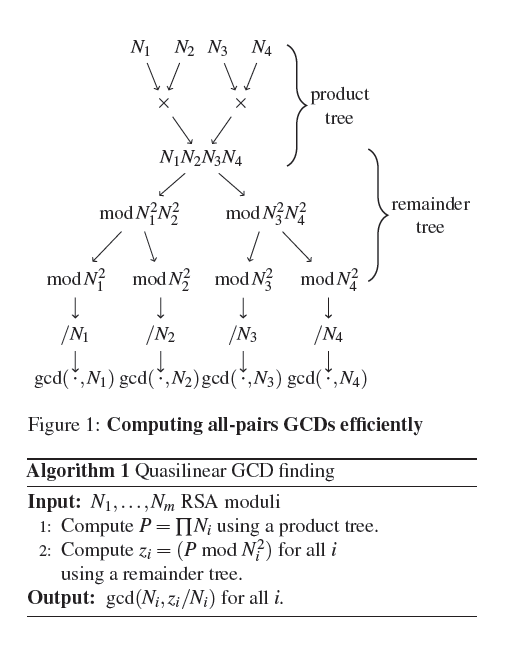
\includegraphics[scale=0.7]{figures/Bernstein_Computing-all-pairs-GCDs.png}
\caption{Algorithmus und Abbildung, um alle ggTs effizient zu berechnen} 
\label{Figure_Bernstein_Computing-all-pairs-GCDs}
\end{center}
\end{figure}


Der Artikel~\cite{nt:Heninger2012} erkl�rt sehr gut \textit{wie} der Algorithmus funktioniert, aber nicht so gut \textit{warum}. Das Produkt $P$ aller Module ist eine sehr gro�e Zahl, sogar wenn man sie mit den einzelnen Modulen vergleicht. Ohne die Vereinfachungen durch den Restebaum w�rde man folgenderma�en vorgehen: Berechnen von $ggT_{i} = ggT( P / m_{i},  m_{i}) $ f�r alle $i$. Vergleichen jedes $ggT_{i} \ne 1$ mit allen anderen $ggT_{j} \ne 1$ mit  $j \ne i$. Wenn zwei ggTs gleich sind, haben ihre Module einen gemeinsamen Faktor.\footnote{%
Eine Voraussetzung daf�r, dass man nur Primfaktoren erh�lt, ist, dass doppelte Module entfernt werden, bevor man den Baum aufsetzt.
}

Weil diese Berechnungen bei den gro�en L�ngenunterschieden der Zahlen sehr langsam sind, wird der Restebaum benutzt. Obwohl es so aussieht, als best�nde er aus mehr Schritte, bedeutet er eine gro�e Vereinfachung.

Innerhalb des Restebaums erh�lt man -- am Ende -- $(P \bmod ({m_{i}^{2}}) ) / m_{i}$ f�r alle $i$.\footnote{%
Es w�rde keinen Sinn machen, beim linken ggT modulo $m_{i}$ statt $m_{i}^{2}$
zu rechnen, denn das bedeutete, $(P \bmod m_{i} ) / m_{i}$ zu benutzen: Denn
$m_{i} | P$, so dass $P/m_{i}$ immer eine ganze Zahl ist, so dass  
$(P \bmod m_{i} )$ immer $= 0$ ist.

\noindent Beispiel mit sehr kleinen Modulen:\\
$ m_{1} = 2*3 = 6;~~~ m_{2} = 2*7 = 14;~~~ P=6*14=84 $\\
$ P \bmod m_{1} = 84 \bmod 6 = 0;~~~ P \bmod {m_{1}^{2}} = 84 \bmod 36 = 12 $\\
$ P \bmod m_{2} = 84 \bmod 14 = 0;~~~ P \bmod {m_{2}^{2}} = 84 \bmod 196 = 84 $\\
$ggT_{1} = ggT(12/6, 6) = ggT(2, 6) = 2 $\\
$ggT_{2} = ggT(84/14, 14) = ggT(6, 14) = 2 $

So wie der Baum strukturiert ist, w�rde es auch keinen Sinn machen, zuerst zu
teilen und dann die Modulo-Operation vorzunehmen, denn das w�rde zu den gegebenen Modulen in umgekehrter Reihenfolge f�hren.

Ebenfalls keinen Sinn w�rde es machen, $(P \bmod ({m_{i}^{3}}) ) / {m_{i}^{2}})$ zu berechnen, da dies nur zus�tzlichen Aufwand ohne Verbesserung bedeutet.
}

Die wesentliche offene Frage ist noch: Warum liefert $ggT((P \bmod {m_{i}^{2}})/ m_{i}, m_{i})$ dasselbe Ergebnis wie $ggT( P / m_{i}, m_{i})$?
Wir beweisen, dass diese Identit�t korrekt ist.\footnote{%
P ist das Produkt aller Module, und $m_{i}$ ist irgendein Modul.
}

$$ggT((P \bmod {m_{i}^{2}})/ m_{i}, m_{i})~~~  \overset{!}{=}  ~~~ggT( P / m_{i}, m_{i})$$
$ \Longleftrightarrow $~~~\footnote{Gem�� Euklids Algorithmus (erste Iteration) ist die folgende Identit�t wahr:\\
$ggT(a, b) = ggT(b, a \bmod b)$ wenn $ b \neq 0 $\\
Dies gilt, weil per Definition gilt: $ggT(a, 0) = a$\\
Angewandt auf unsere Problem bedeutet das:
\mbox{}\\
$ggT((P \bmod {m_{i}^{2}})/ m_{i}, m_{i})=ggT((P \bmod {m_{i}^{2}})/ m_{i} \bmod{m_{i}}, m_{i})$ \mbox{}\\
$ggT( P / m_{i}, m_{i})=ggT( P / m_{i} \bmod{m_{i}}, m_{i})$\mbox{}
}

$$ggT(((P \bmod {m_{i}^{2}})/ m_{i}) \bmod {m_{i}}, m_{i})~~~  \overset{!}{=}  ~~~ggT( (P / m_{i}) \bmod {m_{i}}, m_{i})$$
$ \Longleftrightarrow $~~~\footnote{Die ggTs sind gleich, wenn ihre beiden ersten Argumente gleich sind.
}

$$((P \bmod {m_{i}^{2}})/ m_{i}) \bmod {m_{i}}~~~  \overset{!}{=}  ~~~ (P / m_{i}) \bmod {m_{i}}$$
$ \Longleftrightarrow $~~~\footnote{Die folgenden Umformungen sind �quivalenzumformungen.
}

$$(P \bmod{m_{i}^{2}})/ m_{i} - P / m_{i} \equiv 0   \bmod{m_{i}}~~~ \Leftrightarrow ~~~  m_{i} ~~ | ~~ ((P \bmod{m_{i}^{2}})/ m_{i} - P / m_{i})$$~~~\footnote{%
Benutzt man die Modulo-Operation (Definition \ref{def-zth-remainder} von Seite
\pageref{def-zth-remainder}) und eine Division, ergibt sich:
$~a \bmod{b} ~ =  ~ a - b * \lfloor a/b \rfloor$. So kann $P \bmod{m_{i}^{2}}$ geschrieben werden als $ P-m_{i}^{2} \lfloor P/m_{i}^{2} \rfloor$.
}

$$ m_{i} ~~ | ~~ ((P-m_{i}^{2}* \lfloor P/m_{i}^{2} \rfloor - P))/m_{i}$$~~~\footnote{%
$P$ reduziert sich selbst, der Exponent von $m_{i}$ im Z�hler k�rzt sich mit dem $m_{i}$ im Nenner.
}

$$ m_{i} ~~ | ~~ (m_{i}* \lfloor P/m_{i}^{2} \rfloor)$$

Weil dies offensichtlich wahr ist, k�nnen wir schlie�en, dass die zwei ggTs �quivalent sind.

% yyyyyyyyyyyyyyyyyyyyyyyyyyy
% S�tze und Links:
% https://en.wikipedia.org/wiki/Greatest_common_divisor
% https://de.wikipedia.org/wiki/Gr%C3%B6%C3%9Fter_gemeinsamer_Teiler



% ++++++++++++++++++++++++++++++++++++++++++++++++++++++++++++++++++++++++++
\newpage
\begin{ctsquote}
Viel mehr als unsere F�higkeiten sind es 
unsere Entscheidungen\dots, die zeigen, wer wir wirklich sind.
\caption[Joanne K. Rowling]{Joanne K. Rowling\footnotemark}\index{Rowling, Joanne}
\end{ctsquote}

\addtocounter{footnote}{0}\footnotetext{Joanne K. Rowling, \glqq Harry Potter
und die Kammer des Schreckens\grqq, Carlsen, (c) 1998,
letztes Kapitel \glqq Dobbys Belohnung\grqq, S. 343, Dumbledore.}
% ++++++++++++++++++++++++++++++++++++++++++++++++++++++++++++++++++++++++++
\section{Anwendungen asymmetrischer Kryptographie mit Zahlenbeispielen}

In der modernen Kryptographie \index{Kryptographie!moderne} werden die Ergebnisse
der modularen Arithmetik extensiv angewandt. Hier werden exemplarisch einige
wenige Beispiele aus der Kryptographie mit kleinen\footnote{%
\glqq Klein\grqq~bedeutet beim RSA-Verfahren, dass die Bitl�ngen der Zahlen sehr
viel kleiner sind als $1024$ Bit (das sind $308$ Dezimalstellen). 
$1024$ Bit gilt im Moment in der Praxis als Mindestl�nge f�r sichere RSA-Module.
} Zahlen vorgestellt.

Die Chiffrierung eines Textes besteht darin, dass man aus einer Zeichenkette
(Zahl) durch Anwenden einer Funktion (mathematische Operationen) eine andere
Zahl erzeugt. Dechiffrieren hei�t, diese Funktion umzukehren: aus dem
Zerrbild, das die Funktion aus dem Klartext gemacht hat, das Urbild
wiederherzustellen. Beispielsweise k�nnte der Absender einer vertraulichen
Nachricht zum Klartext $M$ eine geheimzuhaltende Zahl, den Schl�ssel $S$,
addieren und dadurch den Chiffretext $C$ erhalten:
$$ C = M + S. $$
Durch Umkehren dieser Operation, das hei�t durch Subtrahieren von $S$, kann
der Empf�nger den Klartext rekonstruieren:
$$ M = C - S. $$
Das Addieren von $S$ macht den Klartext zuverl�ssig unkenntlich. Gleichwohl
ist diese Verschl�sselung sehr schwach; denn wenn ein Abh�rer auch nur ein
zusammengeh�riges Paar von Klar- und Chiffretext in die H�nde bekommt, kann
er den Schl�ssel berechnen
$$ S = C - M, $$
und alle folgenden mit $S$ verschl�sselten Nachrichten mitlesen. \\
Der wesentliche Grund ist, dass Subtrahieren eine ebenso einfache Operation
ist wie Addieren. 



% --------------------------------------------------------------------------
\hypertarget{OneWayFunktion2}{}%
\subsection{Einwegfunktionen}\index{Einwegfunktion}
\label{OneWayFunktion2}%
Wenn der Schl�ssel auch bei gleichzeitiger Kenntnis von
Klar- und Chiffretext nicht ermittelbar sein soll, braucht man eine
Funktion, die einerseits relativ einfach berechenbar ist - man will ja
chiffrieren k�nnen. Andererseits soll ihre Umkehrung zwar existieren (sonst
w�rde beim Chiffrieren Information verlorengehen), aber de facto
unberechenbar sein.

Was sind denkbare Kandidaten f�r eine solche {\bf Einwegfunktion}?
Man k�nnte an
die Stelle der Addition die Multiplikation setzen; aber schon Grundsch�ler
wissen, dass deren Umkehrung, die Division, nur geringf�gig m�hsamer ist als
die Multiplikation selbst. Man muss noch eine Stufe h�her in der Hierarchie
der Rechenarten gehen: Potenzieren ist immer noch eine relativ einfache
Operation; aber ihre beiden Umkehrungen {\em Wurzelziehen} (finde $b$ in der
Gleichung $a = b^c$ , wenn $a$ und $c$ bekannt sind) und {\em Logarithmieren} (in
derselben Gleichung finde $c$, wenn $a$ und $b$ bekannt sind) sind so kompliziert,
dass ihre Ausf�hrung in der Schule normalerweise nicht mehr gelehrt wird.

W�hrend bei Addition und Multiplikation noch eine gewisse Struktur
wiedererkennbar ist, wirbeln Potenzierung und Exponentiation alle Zahlen
wild durcheinander: Wenn man einige wenige Funktionswerte kennt, wei� man
(anders als bei Addition und Multiplikation) noch kaum etwas �ber die
Funktion im ganzen.



% --------------------------------------------------------------------------
\vskip +10 pt
\subsection{Das Diffie-Hellman Schl�sselaustausch-Protokoll} 
\index{Diffie, Whitfield} 
\index{Hellman, Martin} 
\index{Schl�sselaustausch!Diffie-Hellman}
\index{Diffie-Hellman}

Das DH-Schl�sselaustauschprotokoll (Key Exchange Protocol) wurde 1976 in
Stanford von Whitfield Diffie, Martin E. Hellman und Ralph Merkle erdacht.\footnote{%
  In CT1\index{CrypTool 1} ist dieses Austauschprotokoll visualisiert:
  Sie k�nnen die einzelnen Schritte mit konkreten Zahlen nachvollziehen 
  per Men� {\bf Einzelverfahren \textbackslash{} Protokolle
           \textbackslash{} Diffie-Hellman-Demo}.\\
  In JCT\index{JCrypTool} findet man es in der Standard-Perspektive
  �ber den Men�eintrag {\bf Visualisierungen \textbackslash{} Diffie-Hellman
  Schl�sselaustausch (EC)}.
}

Eine Einwegfunktion dient Alice und Bob\footnote{%
Alice\index{Alice} und Bob\index{Bob} werden standardm��ig als die beiden
berechtigten Teilnehmer eines Protokolls bezeichnet (siehe
\cite[Seite 23]{nt:Schneier1996nt}).
} dazu, sich einen Schl�ssel $S$, den Sessionkey, f�r die nachfolgende
Verst�ndigung zu verschaffen. Dieser ist dann ein Geheimnis, das nur diesen
beiden bekannt ist. Alice w�hlt sich eine Zufallszahl $a$ und h�lt sie geheim.
Aus $a$ berechnet sie mit der Einwegfunktion die Zahl $A = g^a$ und schickt sie
an Bob. Der verf�hrt ebenso, indem er eine geheime Zufallszahl $b$ w�hlt,
daraus $B = g^b$ berechnet und an Alice schickt. Die Zahl $g$ ist beliebig und
darf �ffentlich bekannt sein. Alice wendet die Einwegfunktion mit ihrer
Geheimzahl $a$ auf $B$ an, Bob tut gleiches mit seiner Geheimzahl $b$ und der
empfangenen Zahl $A$.

Das Ergebnis $S$ ist in beiden F�llen dasselbe, weil die Einwegfunktion
kommutativ ist: $g^{a*b} = g^{b*a}$. Aber selbst Bob kann Alices Geheimnis $a$ nicht aus
den ihm vorliegenden Daten rekonstruieren, Alice wiederum Bobs Geheimnis $b$
nicht ermitteln, und ein Lauscher, der $g$ kennt und sowohl $A$ als auch $B$
mitgelesen hat, vermag daraus weder $a$ noch $b$ noch $S$ zu berechnen.

\vskip +10 pt
\input{figures/DH-de.latex}
\vskip +20 pt

\noindent {\bf Ablauf:}\par
\nopagebreak
\noindent Alice und Bob wollen also einen geheimen Sessionkey $S$ �ber einen
abh�rbaren Kanal aushandeln.
\begin{itemize}
   \item[\bf 1.] Sie w�hlen eine Primzahl $p$ und eine Zufallszahl $g$, und tauschen diese
                 Information offen aus.
   \item[\bf 2.] Alice w�hlt nun $a$, eine Zufallszahl kleiner $p$ und
                 h�lt diese geheim.

                 Bob w�hlt ebenso $b$, eine Zufallszahl kleiner $p$ und
                 h�lt diese geheim.
   \item[\bf 3.] Alice berechnet nun $A \equiv g^a {\rm ~(mod~} p)$. \\
                 Bob berechnet $B \equiv g^b {\rm ~(mod~} p)$.
   \item[\bf 4.] Alice sendet das Ergebnis $A$ an Bob. \\
                 Bob sendet das Ergebnis $B$ an Alice.
   \item[\bf 5.] Um den nun gemeinsam zu benutzenden Sessionkey zu bestimmen, 
                 potenzieren sie beide jeweils f�r sich das jeweils empfangene
                 Ergebnis mit ihrer geheimen Zufallszahl modulo $p$. Das hei�t:
         \begin{itemize}
                    \item[-] Alice berechnet $S \equiv B^a {\rm ~(mod~} p)$, und 
                    \item[-] Bob berechnet   $S \equiv A^b {\rm ~(mod~} p)$.
         \end{itemize}
\end{itemize}       
Auch wenn ein Spion $g, p$, und die Zwischenergebnisse $A$ und $B$ abh�rt, kann
er den schlie�lich bestimmten Sessionkey nicht berechnen -- wegen der
Schwierigkeit, den diskreten Logarithmus\footnotemark~zu bestimmen.
\footnotetext{%
Weitere Details zum \index{Logarithmusproblem!diskret}
\hyperlink{HT-Discrete-Logarithm-as-Basis}{Diskreten Logarithmusproblem}
finden Sie in Kapitel~\ref{L-Discrete-Logarithm-as-Basis}.
}

\vskip +10 pt
\noindent Das Ganze soll an einem Beispiel mit (unrealistisch) kleinen Zahlen gezeigt
werden.\vskip +1em

\begin{example}{ mit kleinen Zahlen:}
\begin{itemize}
   \item[\bf 1.] Alice und Bob w�hlen $g = 11$, $p = 347$.
   \item[\bf 2.] Alice w�hlt $a = 240$, Bob w�hlt $b = 39$ und behalten $a$ und $b$ geheim.
   \item[\bf 3.] Alice berechnet $A \equiv g^a \equiv 11^{240} \equiv 49 {\rm ~(mod~} 347).$ \\
                 Bob berechnet $B \equiv g^b \equiv 11^{39} \equiv 285 {\rm ~(mod~} 347).$
   \item[\bf 4.] Alice sendet Bob: $A = 49$, \\
                 Bob sendet Alice: $B = 285$.
   \item[\bf 5.] Alice berechnet $B^a \equiv 285^{240} \equiv 268 {\rm ~(mod~}347),$ \\
                 Bob berechnet $A^b \equiv 49^{39} \equiv 268 {\rm ~(mod~}347)$.
\end{itemize}
Nun k�nnen Alice und Bob mit Hilfe ihres gemeinsamen Sessionkeys sicher
kommunizieren. Auch wenn ein Spion alles, was �ber die Leitung ging, abh�rte:
$g = 11, p = 347, A = 49$ und $B = 285$, den geheimen Schl�ssel kann er nicht
berechnen.
\end{example}

\begin{remark}{:}\\
In diesem Beispiel mit den kleinen Zahlen ist das Diskrete
Logarithmusproblem\index{Logarithmusproblem!diskret} leicht l�sbar, aber mit gro�en
Zahlen ist es kaum zu l�sen.\footnote{%
Mit SageMath\index{SageMath} kann man den diskreten Logarithmus\index{Logarithmusproblem!diskret} $x$,
der die Gleichung $11^x \equiv 49 {\rm ~(mod~}347)$ l�st, folgenderma�en bestimmen
                % $11^x \equiv 49 \pmod{347}$
(hier f�r Allice):
\texttt{discrete\_log(mod(49, 347), mod(11, 347))}. Als Ergebnis erh�lt man $67$.\\
Solche zahlentheoretischen Aufgaben k�nnen auch mit anderen Tools wie PariGP\index{Pari-GP},
LiDIA\index{LiDIA}, BC\index{BC} oder Mathematica\index{Mathematica}
(siehe Anhang Web-Links am Ende dieses Kapitel) gel�st werden:\\
k�nnen solche zahlentheoretischen Aufgaben gel�st werden.\\
- Pari-GP: \texttt{znlog(Mod(49,347),Mod(11,347))}.\\
- LiDIA:   \texttt{dl(11,49,347)}.\\
- Mathematica: Die allgemeine Funktion \glqq Solve\grqq~liefert die {em tdep}-Meldung
  \glqq The equations appear to involve the variables to be solved for in an essentially
    non-algebraic way\grqq.\\
- Mathematica\index{Mathematica}: {\tt MultiplicativeOrder[11, 347, 49]}.\\
Alle liefern das Ergebnis $67$.
}${}^,$\footnote{%
Warum haben die Funktionen f�r den diskreten
Logarithmus\index{DL-Problem}\index{Logarithmusproblem!diskret}\index{diskreter Logarithmus} f�r Alice
den Wert $67$ geliefert und nicht den Wert 240, den Alice als Exponent $a$ w�hlte?\\
Der diskrete Logarithmus ist der kleinste nat�rliche Exponent, der die
Gleichung $11^x \equiv 49{\rm ~(mod~}347)$ l�st. Sowohl $x=67$ als auch $x=240$ (die im Beispiel
gew�hlte Zahl) erf�llen die Gleichung und k�nnen damit zur Berechnung des
Sessionkeys benutzt werden: $285^{240}  \equiv 285^{67} \equiv 268 {\rm ~(mod~}347)$.
H�tten Alice und Bob als Basis $g$ eine Primitivwurzel\index{Primitivwurzel} modulo $p$ gew�hlt,
dann gibt es f�r jeden Rest aus der Menge
$\{1, 2, \cdots, p-1\}$ genau einen Exponenten aus der Menge $\{0, 1, \cdots, p-2\}.$ \\
Info: Zum Modul $347$ gibt es $172$ verschiedene Primitivwurzeln, davon sind $32$
prim (ist nicht notwendig).
Da die im Beispiel f�r $g$ gew�hlte Zahl $11$ keine Primitivwurzel\index{Primitivwurzel}
von $347$ ist, nehmen die Reste nicht alle Werte aus der Menge $\{1, 2, \cdots, 346\}$ an.
Somit kann es f�r einen bestimmten Rest mehr als einen oder auch gar keinen
Exponenten aus der Menge $\{0, 1, \cdots, 345\}$ geben, der die Gleichung
erf�llt. \\
Mit den entsprechenden SageMath-Funktionen\index{SageMath} findet man: \\
\texttt{is\_prime(347)=True}, \texttt{euler\_phi(347)=346}, \texttt{gcd(11,347)=1} und 
\texttt{multiplicative\_order(mod(11, 347))=173}.

\begin{tabular}{|c|c|l|}
\hline
i  & $11^i \bmod 347$ & \\
\hline
      0  &          1   &  \\
      1  &         11   &  \\                                     
      2  &        121   &  \\                                     
      3  &        290   &  \\                                     
     67  &         49   & gesuchter Exponent  \\                    
    172  &        284   &  \\                                                  
    173  &          1   &= Multiplikative Ordnung von $11^i ~(\bmod 347)$  \\ 
    174  &         11   &  \\                                                     
    175  &        121   &  \\                                     
    176  &        290   &  \\                                     
    240  &         49   & gesuchter Exponent  \\                     
\hline
\end{tabular}
\vskip +6 pt

\noindent Weitere Details finden Sie~
in Kapitel~\ref{nt:AppArith3a2} \glqq \nameref{nt:AppArith3a2}\grqq.
}
\end{remark}

\noindent Um die diskreten Logarithen zu erhalten, ist hier Folgendes zu berechnen: \\
Von Alice: $11 ^ x \equiv 49 {\rm ~(mod~}347)$, also $\log_{11}(49) {\rm ~(mod~}347).$\\
Von Bob: $11 ^ y \equiv 285 {\rm ~(mod~}347)$, also $\log_{11}(285){\rm ~(mod~}347)$.



% ++++++++++++++++++++++++++++++++++++++++++++++++++++++++++++++++++++++++++
\newpage
\hypertarget{RSAKonkret}{}%
\hypertarget{Chapter_ElementaryNT_12}{}%ist wahrscheinlich redundant !
\section[Das RSA-Verfahren mit konkreten Zahlen]
	{Das RSA-Verfahren mit konkreten Zahlen\footnotemark}
\footnotetext{%
    \index{SageMath}%
    \index{Nguyen, Minh Van }%
    Weiteres Material: Minh Van Nguyen: \glqq Number Theory and the RSA Public Key
    Cryptosystem. Introductory tutorial on using SageMath to study elementary number
    theory and public key cryptography\grqq, 2009.
    Didaktisch sehr klarer Artikel zu einigen Grundlagen der Zahlentheorie und zur
    Benutzung von SageMath.%\\
%    \url{http://nguyenminh2.googlepages.com/sage_numtheory-rsa.pdf}.%\vskip +3 pt
}
\label{rsaconcrete}\index{RSA}

\begin{ctsquote}
\glqq Das Spiel ist eine Erfindung der Natur, um uns auf schwierige Realit�ten vorzubereiten. Sind Sie jetzt endlich bereit, der Realit�t ins Auge zu sehen, Sergeant?\grqq 
\caption[Daniel Suarez]{Daniel Suarez\footnotemark}\index{Suarez, Daniel}
%Der erste String nach \caption geht in das Zitate-Verzeichnis.
\end{ctsquote}
\addtocounter{footnote}{0}\footnotetext{Daniel Suarez, \glqq Daemon\grqq, rororo, (c) 2010,
Kapitel 45, \glqq Wiedereintritt\grqq, S. 615, Sobol.}

Nachdem oben die \hyperlink{RSA}{Funktionsweise des RSA-Verfahrens} beschrieben
wurde, sollen diese Schritte hier mit konkreten, aber kleinen Zahlen
durchgef�hrt werden.


% --------------------------------------------------------------------------
\subsection{RSA mit kleinen Primzahlen und mit einer Zahl als Nachricht}
Bevor wir RSA auf einen Text anwenden, wollen wir es erst direkt mit einer
Zahl zeigen.\footnote{%
   Mit CT1\index{CrypTool 1} k�nnen Sie dies per Men� {\bf Einzelverfahren
   \textbackslash{} RSA-Kryptosystem \textbackslash{} RSA-Demo} l�sen.
}
\begin{itemize}
  \item[\bf 1.] Die gew�hlten Primzahlen seien $p=5$ und $q=11$. \\
                Also ist $n=55$ und $J(n) = (p-1)*(q-1)=40$.
  \item[\bf 2.] $e = 7$ ($e$ sollte\footnote{%
                Siehe Fu�note~\ref{foot:Selection-of-e} auf Seite
                \pageref{foot:Selection-of-e}.} zwischen $11$ und $39$ liegen,
                und muss teilerfremd\index{Zahlen!teilerfremde (co-prime)}
                zu $40$ sein).
  \item[\bf 3.] $d = 23$ (da $23*7 \equiv 161 \equiv 1{\rm ~(mod~}40)$)
  \begin{itemize} 
     \item[] $\rightarrow$ Public-Key des Empf�ngers: $(55, 7),$
     \item[] $\rightarrow$ Private-Key des Empf�ngers: $(55, 23).$ 
  \end{itemize}
  \item[\bf 4.] Nachricht sei nur die Zahl $M = 2$ (also ist kein
                Aufbrechen in Bl�cke n�tig).
  \item[\bf 5.] Verschl�sseln: $C \equiv 2^7 \equiv 18 {\rm ~(mod~}55).$
  \item[\bf 6.] Chiffrat ist nur die Zahl $C = 18$ (also kein Aufbrechen
                in Bl�cke n�tig).
  \item[\bf 7.] Entschl�sseln: $M \equiv 18^{23} \equiv 18^{(1+2+4+16)} \equiv 18*49*36*26 \equiv 2 {\rm ~(mod~}55).$
\end{itemize}
Nun wollen wir RSA auf einen Text anwenden: zuerst mit dem
Gro�buchstabenalphabet (26 Zeichen), dann mit dem gesamten
ASCII-Zeichensatz als Bausteine f�r die Nachrichten.


% --------------------------------------------------------------------------
\subsection{RSA mit etwas gr��eren Primzahlen und einem Text aus Gro�buchstaben}\label{rsaex2}
Gegeben ist der Text \glqq ATTACK AT DAWN\grqq, und die Zeichen werden gem�� 
Tabelle~\ref{alphacode}\index{Blockl�nge} codiert.\footnote{%
Mit CT1\index{CrypTool 1} k�nnen Sie dies per Men� 
{\bf Einzelverfahren \textbackslash{} RSA-Kryptosystem \textbackslash{} RSA-Demo} l�sen. Dies ist auch im Tutorial/Szenario der Online-Hilfe zu CT1 beschrieben [Optionen,
Alphabet vorgeben, Basissystem, Blockl�nge\index{Blockl�nge} 2 und Dezimaldarstellung].
}

\begin{table}[ht]
\begin{center}
\begin{tabular}{|c|l||c|l|}
\hline
Zeichen & Zahlenwert & Zeichen & Zahlenwert \\
\hline
\hline
Blank    & 0   & M  & 13 \\
A        & 1   & N    & 14 \\ 
B        & 2   & O    & 15 \\ 
C        & 3   & P    & 16 \\  
D        & 4   & Q    & 17 \\ 
E        & 5   & R    & 18 \\ 
F        & 6   & S    & 19 \\  
G        & 7   & T    & 20 \\  
H        & 8   & U    & 21 \\ 
I        & 9   & V    & 22 \\   
J       & 10   & W    & 23 \\  
K       & 11   & X    & 24 \\ 
L       & 12   & Y    & 25 \\
&              & Z    & 26 \\
\hline
\end{tabular} 
\end{center}
\hypertarget{Grossbuchstaben-Alphabet}{}
\caption{Gro�buchstabenalphabet}\index{Gro�buchstabenalphabet}
\label{alphacode}
\end{table}

\noindent {\bf Schl�sselerzeugung (Schritt 1 bis 3):} \\
%\vskip 5 pt
{\bf 1.} $p=47, q=79$ $( n= 3713;~ J(n) = (p-1)*(q-1)=3588).$ \\
{\bf 2.} $e=37$ ($e$ sollte\footnote{%
                Siehe Fu�note~\ref{foot:Selection-of-e} auf Seite
                \pageref{foot:Selection-of-e}.}  zwischen 79 und 3587 liegen,
                und muss teilerfremd\index{Zahlen!teilerfremde (co-prime)}
                zu $3588$ sein). \\
{\bf 3.} $d=97$ (denn $e*d=1{\rm ~mod~}J(n); 37*97 \equiv 3589 
\equiv 1{\rm ~(mod~}3588) \;$).\footnote{%
  Wie man $d = 97$ mit Hilfe des erweiterten ggT berechnet, wird in
  Anhang~\ref{nt:NumberTheory_Appendix_GCD} gezeigt.
}

\noindent {\bf 4. Verschl�sselung:} \\ 
{\tt
\begin{tabular}{rcccccccccccccccccccc}
{\rm Text:} & A & T & T & A & C & K & & A & T &  & D & A & W & N \\
{\rm Zahl:} & 01 & 20 & 20 & 01 & 03 & 11 & 00 & 01 & 20 & 00 & 04 & 01 & 23 & 14
\end{tabular}
}
\index{Blockl�nge}

\noindent Aufteilung dieser 28-stelligen Zahl in 4-stellige Teile (denn $2626$ ist noch kleiner als $n=3713$), d.h. dass
die Blockl�nge 2 betr�gt.\\
{\tt 0120 2001 0311 0001 2000 0401 2314}

\label{SrcArith4a}
\noindent Verschl�sselung aller 7 Teile jeweils per: $C \equiv M^{37}{\rm ~(mod~3713)}$:\footnote{%
  In Kapitel~\ref{nt:AppArith4a} \glqq \nameref{nt:AppArith4a}\grqq~
  finden Sie den Beispiel-Quelltext zur RSA-Verschl�sselung mit SageMath.
} \\
{\tt 1404 2932 3536 0001 3284 2280 2235}

\noindent {\bf 5. Entschl�sselung:} \\ 
Chiffrat: {\tt 1404 2932 3536 0001 3284 2280 2235 }

\noindent Aufteilung dieser 28-stelligen Zahl in 4-stellige Teile.

\noindent Entschl�sselung aller $7$ Teile jeweils per: $M \equiv C^{97}{\rm ~(mod~}3713)$: \\
{\tt 0120 2001 0311 0001 2000 0401 2314}

\noindent Umwandeln von 2-stelligen Zahlen in Gro�buchstaben und Blanks.

\noindent Bei den gew�hlten Werten ist es f�r einen Kryptoanalytiker
\index{Kryptoanalyse} einfach, aus den �ffentlichen Parametern
$n=3713$ und $e=37$ die geheimen Werte zu finden, indem
er offenlegt, dass $3713 = 47 * 79$.

\noindent Wenn $n$ eine $1024$-Bit-Zahl ist, bestehen daf�r -- nach heutigen
Kenntnissen -- wenig Chancen.


% --------------------------------------------------------------------------
\subsection[RSA mit noch etwas gr��eren Primzahlen und ASCII-Zeichen]{RSA mit noch etwas gr��eren Primzahlen und mit einem Text aus ASCII-Zeichen}

Real wird das ASCII-Alphabet benutzt, um die Einzelzeichen der Nachricht in
8-Bit lange Zahlen zu codieren. 

\noindent Diese Aufgabe\footnote{%
Mit CT1\index{CrypTool 1} k�nnen Sie diese Aufgabe per Men� 
{\bf Einzelverfahren \textbackslash{} RSA-Kryptosystem \textbackslash{}
 RSA-Demo} l�sen.\\
Mit JCT\index{JCrypTool} k�nnen Sie diese Aufgabe im Men�
{\bf Visualisierungen \textbackslash{} RSA-Kryptosystem}
der Standard-Perspektive l�sen.%xxxxxxxxxxxxxxxxxxxxxxxxxxxxxxxxxxxx
} 
ist angeregt durch das Beispiel aus \cite[S. 271]{nt:Eckert2003}. 
\index{Eckert 2003}
% Eigentlich stammte die Aufgabe aus Eckert2001, S. 215. Diese 1. Buchausgabe
% ist nun nicht mehr im Literaturverzeichnis (6.6.2, Das RSA-Verfahren,
% Bsp. 6.14 (ASCII-Codierung).
% In Eckert2001 passten nur die Zahlen nicht ganz, so dass ich andere
% w�hlte bei gl. Text. In Eckert 2003 sind nochmal andere Zahlen,
% aber ich lie� das Skript unver�ndert.

\noindent Der Text \glqq RSA works!\grqq~bedeutet in Dezimalschreibweise codiert: 

{\tt
\begin{tabular}{rcccccccccccccccccccc}
{\rm Text:} & R & S & A &   & w & o & r & k & s & ! \\
{\rm Zahl:} & 82 & 83 & 65 & 32 & 119 & 111 & 114 & 107 & 115 & 33 
\end{tabular} } % \tt

\noindent Das Beispiel wird in 2 Varianten durchgespielt. Gemeinsam f�r beide sind die Schritte $1$ bis $3$.
\vskip +10pt
\noindent {\bf Schl�sselerzeugung (Schritt 1 bis 3):} \\\label{SrcArith4b}%
{\bf 1.} $p=509,~q=503 \quad (n= 256.027; \; ~J(n)=(p-1)*(q-1)=255.016=2^3*127*251)$.\footnote{%
  In Kapitel~\ref{nt:AppArith4b} \glqq \nameref{nt:AppArith4b}\grqq~
  finden Sie den Quelltext zur Faktorisierung von $J(n)$ mit SageMath.
} \\
{\bf 2.} $e=65.537$ ($e$ sollte\footnote{%
                Siehe Fu�note~\ref{foot:Selection-of-e} auf Seite
                \pageref{foot:Selection-of-e}.}
                zwischen $509$ und $255.015$ liegen, u. muss\footnote{%
                $e$ darf also nicht $2, 127$ oder $251$ sein
                ($65537 = 2^{16}+1$) ($255,016 = 2^{3}*127*251$).\\
                Real wird $J(n)$ nicht faktorisiert, sondern f�r das gew�hlte
                $e$ wird mit dem Euklidschen Algorithmus sichergestellt, dass
                ggT$(e,J(n))=1$.
                }
      teilerfremd\index{Zahlen!teilerfremde (co-prime)} zu $255.016$ sein).\\
{\bf 3.} $d=231.953$ \\
\strut\quad\ (denn $e \equiv d^{-1}{\rm ~mod~}J(n);$
\mbox{}\quad $65.537*231.953 \equiv 15.201.503.761 \equiv 1
{\rm ~(mod~}255.016))$.\footnote{%
Andere m�gliche Kombinationen von (e,d) sind z.B.: (3, 170.011), (5, 204.013), (7, 36.431).
}


% --------------------------------------------------------------------------
\subsection*{Variante 1:\\ ASCII-Zeichen werden einzeln ver- und entschl�sselt (keine Blockbildung).} 

{\bf 4. Verschl�sselung:} \\ 
{\tt
\begin{tabular}{rcccccccccccccccccccc}
{\rm Text:} & R & S & A &   & w & o & r & k & s & ! \\
{\rm Zahl:} & 82 & 83 & 65 & 32 & 119 & 111 & 114 & 107 & 115 & 33 
\end{tabular} } % \tt

\noindent Keine Zusammenfassung der Buchstaben!\footnote{%
F�r sichere Verfahren braucht man gro�e Zahlen, die m�glichst alle Werte bis
$n-1$ annehmen. Wenn die m�gliche Wertemenge der Zahlen in der Nachricht zu
klein ist, nutzen auch gro�e Primzahlen nichts f�r die Sicherheit.
Ein ASCII-Zeichen ist durch $8$ Bits repr�sentiert. Will man gr��ere Werte,
muss man mehrere Zeichen zusammenfassen. Zwei Zeichen ben�tigen 16 Bit, womit
maximal der Wert 65.536 darstellbar ist; dann muss der Modul $n$ gr��er sein als
$2^{16} = 65.536$. Dies wird in Variante 2 angewandt.
Beim Zusammenfassen bleiben in der Bin�r-Schreibweise die f�hrenden Nullen
erhalten (genauso wie wenn man oben in der Dezimalschreibweise alle Zahlen
3-stellig schreiben w�rde und dann die Folge {\tt 082 083, 065 032,
119 111, 114 107, 115 033} h�tte). 
}
\label{SrcArith4c}\\
Verschl�sselung pro Zeichen per: $C \equiv M^{65.537}{\rm ~(mod~}256.027)$:\footnote{%
  In Kapitel~\ref{nt:AppArith4c} \glqq \nameref{nt:AppArith4c}\grqq~
  finden Sie den Quelltext zur RSA-Exponentiation mit SageMath.
}\\
{\tt
\begin{tabular}{lllll}
212984 & 025546 & 104529 & 031692 & 248407 \\
100412 & 054196 & 100184 & 058179 & 227433\\
\end{tabular} 
}

\noindent {\bf 5. Entschl�sselung:}\\
Chiffrat: \\ 
{\tt
\begin{tabular}{lllll}
212984 & 025546 & 104529 & 031692 & 248407 \\
100412 & 054196 & 100184 & 058179 & 227433\\
\end{tabular} }

\noindent Entschl�sselung pro Zeichen per: $M \equiv C^{231.953}{\rm ~mod~}256.027$: \\
{\tt 82 83 65 32 119 111 114 107 115 33}\\


% --------------------------------------------------------------------------
\subsection*{Variante 2:\\ Jeweils zwei ASCII-Zeichen werden als Block ver- und entschl�sselt.} 

Bei der Variante 2 wird die Blockbildung in zwei verschiedenen Untervarianten 4./5. und 4'./5'. dargestellt.

{\tt
\begin{tabular}{rcccccccccccccccccccc}
{\rm Text:} & R & S & A &   & w & o & r & k & s & ! \\
{\rm Zahl:} & 82 & 83 & 65 & 32 & 119 & 111 & 114 & 107 & 115 & 33 
\end{tabular} } % \tt

\noindent {\bf 4. Verschl�sselung:} \\
Blockbildung\footnote{%
\\ \tt \begin{tabular}{ll@{ }l@{ }l}
Einzelzeichen& Bin�rdarstellung  &&Dezimaldarstellung\\
01010010, 82 & 01010010 01010011 & = &21075 \\
01010011, 83 & \\
01000001, 65 & 01000001 00100000 & = &16672  \\
00100000, 32  \\
01110111, 119 & 01110111 01101111 & = &30575 \\
01101111, 111 \\ 
01110010, 114 & 01110010 01101011 & = &29291 \\
01101011, 107 \\
01110011, 115 & 01110011 00100001 & = &29473 \\
00100001, 33: 
\end{tabular}
} (die ASCII-Zeichen werden als 8-stellige Bin�rzahlen hintereinander geschrie"-ben):\\
{\tt 21075 16672 30575 29291 29473}\footnote{%
Mit CT1\index{CrypTool 1} k�nnen Sie dies per Men� {\bf Einzelverfahren \textbackslash{}
RSA-Kryptosystem \textbackslash{} RSA-Demo} mit den folgenden Optionen l�sen: alle
$256$ Zeichen, b-adisch, Blockl�nge\index{Blockl�nge} 2, dezimale Darstellung.
}

\label{SrcArith4d}
\noindent Verschl�sselung pro Block per: $C \equiv M^{65.537}{\rm ~(mod~}256027)$:\footnote{%
  In Kapitel~\ref{nt:AppArith4d} \glqq \nameref{nt:AppArith4d}\grqq~
  finden Sie den Quelltext zur RSA-Exponentiation mit SageMath.
} \\
{\tt 158721 137346 37358 240130 112898}

\noindent {\bf 5. Entschl�sselung:} \\
Chiffrat: \\
{\tt 158721 137346 37358 240130 112898}

\noindent Entschl�sselung pro Block per: $M \equiv C^{231.953}{\rm ~(mod~}256.027)$: \\
{\tt 21075 16672 30575 29291 29473}

\vskip +10 pt
%{\bf Umwandeln:} jeden Block bin�r in 2 Zahlen; danach jede Zahl in ASCII-Zeichen.

\noindent {\bf 4'. Verschl�sselung:} \\
Blockbildung (die ASCII-Zeichen werden als 3-stellige Dezimalzahlen hintereinander geschrie"-ben): \\
{\tt 82083 65032 119111 114107 115033}\footnote{%
Die RSA-Verschl�sselung mit dem Modul $n=256.027$ ist bei dieser Einstellung korrekt,
da die ASCII-Bl�cke in Zahlen kleiner oder gleich $255.255$ kodiert werden.
} 

\label{SrcArith4e}
\noindent Verschl�sselung pro Block per: $C \equiv M^{65537}{\rm ~(mod~}256.027)$:\footnote{%
  In Kapitel~\ref{nt:AppArith4e} \glqq \nameref{nt:AppArith4e}\grqq~
  %%xIn \hyperlink{nt:AppArith4e}{Anhang zu diesem Kapitel}
  finden Sie den Quelltext zur RSA-Exponentiation mit SageMath.
} \\ 
{\tt 198967 051405 254571 115318 014251}

\noindent {\bf 5'. Entschl�sselung:} \\
Chiffrat: \\
{\tt 198967 051405 254571 115318 014251}

\noindent Entschl�sselung pro Block per: $M \equiv C^{231.953}{\rm ~(mod~}256.027)$: \\
{\tt 82083 65032 119111 114107 115033} 



% --------------------------------------------------------------------------
\subsection{Eine kleine RSA-Cipher-Challenge (1)}
\index{RSA!Cipher-Challenge}
Die Aufgabe stammt aus \cite[Exercise 4.6]{nt:3Stinson1995}\index{Stinson 1995}:
Prof. Stinson hat dazu eine L�sung ver�ffentlicht.\footnote{%
\url{http://www.cacr.math.uwaterloo.ca/~dstinson/solns.html} oder
\url{http://bibd.unl/~stinson/solns.html}
}
Es geht aber nicht nur um das Ergebnis, sondern vor allem
um die Einzelschritte der L�sung, also um die Darlegung der
Kryptoanalyse\index{Kryptoanalyse}.\footnote{%
Im Szenario der Online-Hilfe zu CT1\index{CrypTool 1} und in der
Pr�sentation auf der CT-Webseite wird der L�sungsweg skizziert.
Wenn uns jemand einen (weiteren) gut aufbereiteten konkreten L�sungsweg
schickt, nehmen wir ihn gerne in die Dokumentation auf.
}

\noindent Hier die Aufgabe im Originaltext:

Two samples of RSA ciphertext are presented in Tables~\ref{stinson1}\footnote{%
Die Zahlen dieser Tabelle k�nnen Sie mit Copy und Paste weiter bearbeiten.
}
and \ref{stinson2}\footnote{%
Die Zahlen dieser Tabelle befinden sich auch in der Online-Hilfe zu
CT1\index{CrypTool 1} im Kapitel \glqq Szenario f�r die RSA-Demonstration\grqq.
}.
Your task is to decrypt them. The public parameters of the system are 

\noindent $n = 18.923$ and $e = 1261$ (for Table~\ref{stinson1}) and \\
\noindent $n = 31.313$ and $e = 4913$ (for Table~\ref{stinson2}).

This can be accomplished as follows. First, factor $n$ (which is easy
because it is so small). Then compute the exponent $d$ from $J(n)$, and,
finally, decrypt the ciphertext. Use the square-and-multiply
\index{Square and multiply} algorithm to exponentiate modulo $n$.

In order to translate the plaintext back into ordinary English text, you
need to know how alphabetic characters are ''encoded'' as elements in
$\mathbb{Z}_n$. Each element of $\mathbb{Z}_n$ represents three alphabetic
characters as in the following examples: 

{\tt \begin{tabular}{lll}
DOG & $\mapsto$ & $3 * 26^2 + 14 * 26 + 6= 2398$ \\
CAT & $\mapsto$ & $2 * 26^2 + 0 * 26 + 19 = 1371$ \\
ZZZ & $\mapsto$ & $25 * 26^2 + 25 * 26 + 25 = 17.575$. 
\end{tabular} }

You will have to invert this process as the final step in your program.

The first plaintext was taken from ''The Diary of Samuel Marchbanks'', by
Robertson Davies, 1947, and the second was taken from ''Lake Wobegon Days'',
by Garrison Keillor, 1985.

\begin{table}[ht]
{\tt 
\begin{tabular}{llllllll}
12423 & 11524  & 7243  & 7459 & 14303  & 6127 & 10964 & 16399 \\
 9792 & 13629 & 14407 & 18817 & 18830 & 13556  & 3159 & 16647 \\
 5300 & 13951    & 81  & 8986  & 8007 & 13167 & 10022 & 17213 \\
 2264   & 961 & 17459  & 4101  & 2999 & 14569 & 17183 & 15827 \\
12693  & 9553 & 18194  & 3830  & 2664 & 13998 & 12501 & 18873 \\
12161 & 13071 & 16900  & 7233  & 8270 & 17086  & 9792 & 14266 \\
13236  & 5300 & 13951  & 8850 & 12129  & 6091 & 18110  & 3332 \\
15061 & 12347  & 7817  & 7946 & 11675 & 13924 & 13892 & 18031 \\
 2620  & 6276  & 8500   & 201  & 8850 & 11178 & 16477 & 10161 \\
 3533 & 13842  & 7537 & 12259 & 18110    & 44  & 2364 & 15570 \\
 3460  & 9886  & 8687  & 4481 & 11231  & 7547 & 11383 & 17910 \\
12867 & 13203  & 5102  & 4742  & 5053 & 15407  & 2976  & 9330 \\
12192    & 56  & 2471 & 15334   & 841 & 13995 & 17592 & 13297 \\
 2430  & 9741 & 11675   & 424  & 6686   & 738 & 13874  & 8168 \\
 7913  & 6246 & 14301  & 1144  & 9056 & 15967  & 7328 & 13203 \\
  796   & 195  & 9872 & 16979 & 15404 & 14130  & 9105  & 2001 \\
 9792 & 14251  & 1498 & 11296  & 1105  & 4502 & 16979  & 1105 \\
   56  & 4118 & 11302  & 5988  & 3363 & 15827  & 6928  & 4191 \\
 4277 & 10617   & 874 & 13211 & 11821  & 3090 & 18110    & 44 \\
 2364 & 15570  & 3460  & 9886  & 9988  & 3798  & 1158  & 9872 \\
16979 & 15404  & 6127  & 9872  & 3652 & 14838  & 7437  & 2540 \\
 1367  & 2512 & 14407  & 5053  & 1521   & 297 & 10935 & 17137 \\
 2186  & 9433 & 13293  & 7555 & 13618 & 13000  & 6490  & 5310 \\
18676  & 4782 & 11374   & 446  & 4165 & 11634  & 3846 & 14611 \\
 2364  & 6789 & 11634  & 4493  & 4063  & 4576 & 17955  & 7965 \\
11748 & 14616 & 11453 & 17666   & 925    & 56  & 4118 & 18031 \\
 9522 & 14838  & 7437  & 3880 & 11476  & 8305  & 5102  & 2999 \\
18628 & 14326  & 9175  & 9061   & 650 & 18110  & 8720 & 15404 \\
 2951   & 722 & 15334   & 841 & 15610  & 2443 & 11056  & 2186 
\end{tabular} } % tt
\caption{RSA-Geheimtext A}
\label{stinson1}
\end{table}

\begin{table}[ht]
{\tt 
\begin{tabular}{llllllll}
 6340  & 8309 & 14010  & 8936 & 27358 & 25023 & 16481 & 25809 \\
23614  & 7135 & 24996 & 30590 & 27570 & 26486 & 30388  & 9395 \\
27584 & 14999  & 4517 & 12146 & 29421 & 26439  & 1606 & 17881 \\
25774  & 7647 & 23901  & 7372 & 25774 & 18436 & 12056 & 13547 \\
 7908  & 8635  & 2149  & 1908 & 22076  & 7372  & 8686  & 1304 \\
 4082 & 11803  & 5314   & 107  & 7359 & 22470  & 7372 & 22827 \\
15698 & 30317  & 4685 & 14696 & 30388  & 8671 & 29956 & 15705 \\
 1417 & 26905 & 25809 & 28347 & 26277  & 7897 & 20240 & 21519 \\
12437  & 1108 & 27106 & 18743 & 24144 & 10685 & 25234 & 30155 \\
23005  & 8267  & 9917  & 7994  & 9694  & 2149 & 10042 & 27705 \\
15930 & 29748  & 8635 & 23645 & 11738 & 24591 & 20240 & 27212 \\
27486  & 9741  & 2149 & 29329  & 2149  & 5501 & 14015 & 30155 \\
18154 & 22319 & 27705 & 20321 & 23254 & 13624  & 3249  & 5443 \\
 2149 & 16975 & 16087 & 14600 & 27705 & 19386  & 7325 & 26277 \\
19554 & 23614  & 7553  & 4734  & 8091 & 23973 & 14015   & 107 \\
 3183 & 17347 & 25234  & 4595 & 21498  & 6360 & 19837  & 8463 \\
 6000 & 31280 & 29413  & 2066   & 369 & 23204  & 8425  & 7792 \\
25973  & 4477 & 30989                               
\end{tabular} } % tt
\caption{RSA-Geheimtext B}
\label{stinson2}
\end{table}


% --------------------------------------------------------------------------
\clearpage
\subsection{Eine kleine RSA-Cipher-Challenge (2)}
\index{RSA!Cipher-Challenge}

Die folgende Aufgabe ist eine korrigierte Variante aus dem Buch
von Prof.~Yan \cite[Example 3.3.7, S. 318]{nt:Yan2000}. \index{Yan 2000}
Es geht aber nicht nur um das Ergebnis, sondern vor allem um die
Einzelschritte der L�sung, also um die Darlegung der 
Kryptoanalyse\index{Kryptoanalyse}.\footnote{%
Im Szenario der Online-Hilfe zu CT1\index{CrypTool 1} und in der 
CrypTool-Pr�sentation werden der L�sungsweg skizziert. 
Wenn uns jemand einen gut aufbereiteten konkreten L�sungsweg schickt, 
nehmen wir ihn gerne in die Dokumentation auf.
}

Man kann sich drei v�llig unterschiedlich schwierige Aufgaben vorstellen:
Gegeben ist jeweils der Geheimtext und der �ffentliche Schl�ssel $(e,n)$:
\begin{itemize}
\item \index{Angriff!Known-Plaintext} Known-Plaintext: finde den geheimen Schl�ssel $d$ unter Benutzung der
zus�tzlich bekannten Ursprungsnachricht.
\item \index{Angriff!Ciphertext-only} Ciphertext-only: finde $d$ und die Klartextnachricht.
\item \index{Faktorisierung!Faktorisierungsproblem} RSA-Modul knacken, d.h. faktorisieren (ohne Kenntnis der Nachrichten).
\end{itemize}

%\newpage
$n = 63978486879527143858831415041, ~e = 17579$

Klartextnachricht\footnote{%
Die Zahlen dieser Tabelle befinden sich auch in der Online-Hilfe zu
CT1\index{CrypTool 1} im Kapitel \glqq Szenario f�r die RSA-Demonstration\grqq.
}:

{\tt
\begin{tabular}{l}
1401202118011200, \\
1421130205181900, \\
0118050013010405, \\
0002250007150400 
\end{tabular} } % tt

Geheimtext:

{\tt
\begin{tabular}{l}
45411667895024938209259253423, \\
16597091621432020076311552201, \\
46468979279750354732637631044, \\
32870167545903741339819671379
\end{tabular} } % tt
\vskip +8pt

\begin{remark}{:}\\
Die urspr�ngliche Nachricht bestand aus einem Satz mit 31 Zeichen (codiert
mit dem Gro�buchstabenalphabet\index{Gro�buchstabenalphabet} aus Abschnitt~\ref{rsaex2}).
ann wurden je 16 Dezimalziffern zu
einer Zahl zusammengefasst (die letzte Zahl wurde mit Nullen aufgef�llt).
Diese Zahlen wurden mit $e$ potenziert.
\end{remark}

Beim Entschl�sseln ist darauf zu achten, dass die berechneten Zahlen vorne
mit Nullen aufzuf�llen sind, um den Klartext zu erhalten.

Wir betonen das, weil in der Implementierung und Standardisierung die Art
des Padding sehr wichtig ist f�r interoperable Algorithmen.








% ---------------------------------------------------------------------------
% ---------------------------------------------------------------------------

% ++++++++++++++++++++++++++++++++++++++++++++++++++++++++++++++++++++++++++
\newpage
\hypertarget{nt:NumberTheory_Appendix_GCD}{}
\section[Anhang: Der ggT und die beiden Algorithmen von Euklid]
        {Anhang: Der gr��te gemeinsame Teiler (ggT) von ganzen Zahlen und die beiden
	 Algorithmen von Euklid\footnotemark}
\footnotetext{%
    \index{ZT, Lernprogramm Zahlentheorie}%
    \index{Lernprogramm ZT}%
Mit dem Zahlentheorie-Lernprogramm {\bf ZT} k�nnen Sie sehen,\\
a) wie Euklids Algorithmus den ggT berechnet (Lern-Kapitel 1.3, Seiten 14-19/21) und \\
b) wie Euklids erweiterter Algorithmus das multiplikative Inverse findet
   (Lern-Kapitel 2.2, Seite 13/40).\\
ZT k�nnen Sie in CT1\index{CrypTool 1} �ber das Men�
{\bf Einzelverfahren \textbackslash{} Zahlentheorie interaktiv \textbackslash{}
Lernprogramm f�r Zahlentheorie} aufrufen.
Siehe Anhang~\ref{s:appendix-Learn-NT}.\\
    CT2\index{CrypTool 2} enth�lt in dem Krypto-Tutorial-Pfad
    \glqq {\bf Welt der Primzahlen} $\Rightarrow$ Zahlentheorie
    $\Rightarrow$ Zahlentheoretische Funktionen\grqq~die Funktionen
    \glqq Erweiterter euklidischer Algorithmus\grqq~und
    \glqq Modulare multiplikative Inverse\grqq.
}
\label{nt:NumberTheory_Appendix_GCD}
\index{Euklidscher Algorithmus!erweiterter}
\index{ggT}

%%%\item
Der gr��te gemeinsame Teiler zweier nat�rlicher Zahlen $a$ und $b$ ist eine
wichtige Gr��e, die sehr schnell berechnet werden kann. Wenn eine Zahl $c$ die
Zahlen $a$ und $b$ teilt (d.h. es gibt ein $a'$ und ein $b'$, so dass
$a = a'*c$ und $b = b'*c$), dann teilt $c$ auch den Rest $r$ der Division von
$a$ durch $b$. Wir schreiben in aller K�rze:
Aus $c$ teilt $a$ und $b$ folgt:
$c$ teilt $r = a - \lfloor a/b \rfloor * b$.\footnote{\label{nt_Gauss-Klammer}%
Die untere Gaussklammer \index{Gaussklammer} $\lfloor x \rfloor $ der
reellwertigen Zahl $x$ ist definiert als: $\lfloor x \rfloor $ ist die gr��te
ganze Zahl kleiner oder gleich $x$.\\
Vergleiche Fu�note~\ref{nt_Gauss-Funktion} auf Seite ~\pageref{nt_Gauss-Funktion}.
%aaaaaaaaaaaa
}

Weil die obige Aussage f�r alle gemeinsamen Teiler $c$ von $a$ und $b$ gilt,
folgt f�r den gr��ten gemeinsamen Teiler von $a$ und $b$ (ggT($a,b$)) die
Aussage $$ {\rm ggT}(a,b) = {\rm ggT}(a - \lfloor a/b \rfloor * b, b). $$
Mit dieser Erkenntnis l�sst sich der Algorithmus zum Berechnen des ggT zweier
Zahlen wie folgt (in Pseudocode) beschreiben:

\begin{verbatim}
INPUT: a,b != 0
1. if ( a < b ) then  x = a; a = b; b = x; // Vertausche a und b (a > b)
2. a = a - int(a/b) * b        // a wird kleiner b, der ggT(a, b) 
                               // bleibt unver�ndert 
3. if ( a != 0 ) then goto 1.  // nach jedem Schritt f�llt a, und 
                               // der Algorithmus endet, wenn a == 0.
OUTPUT "ggT(a,b) = " b         // b ist der ggT vom urspr�nglichen a und b
\end{verbatim}

%%%\item 
Aus dem ggT lassen sich aber noch weitere Zusammenh�nge bestimmen:
Dazu betrachtet man f�r $a$ und $b$ das Gleichungssystem:
\begin{eqnarray*}
 a & = & 1*a + 0*b \nonumber \\
 b & = & 0*a + 1*b, \nonumber
\end{eqnarray*}
bzw. in Matrix-Schreibweise:
$$ \left(\begin{array}{c}a \\ b\end{array}\right) = 
   \left(\begin{array}{cc} 1 & 0 \\ 0 & 1 \end{array}\right) *
   \left(\begin{array}{c} a \\ b \end{array} \right).$$
Wir fassen diese Informationen in der erweiterten Matrix 
$$\left(\begin{array}{cccc} a & | & 1 & 0 \\ b & | & 0 & 1 \end{array} \right)$$
zusammen. Wendet man den ggT-Algorithmus auf diese Matrix an, so erh�lt man den 
{\em erweiterten Euklidschen Algorithmus},  mit dem die multiplikative Inverse bestimmt wird. 
\index{Euklidscher Algorithmus!erweiterter}

\newpage
\noindent {\tt INPUT:} $a,b \not= 0$
\begin{itemize}
  \item[\tt 0.] $x_{1,1} := 1, x_{1,2} := 0, x_{2,1} := 0, x_{2,2} := 1$
  \item[\tt 1.] $ \left(\begin{array}{cccc} a & | & x_{1,1} & x_{1,2} \\ b & | & x_{2,1} & x_{2,2} \end{array} \right) := 
           \left(\begin{array}{cc} 0 & 1  \\ 1 & - \lfloor a/b \rfloor * b \end{array} \right)*
           \left(\begin{array}{cccc} a & | & x_{1,1} & x_{1,2} \\ b & | & x_{2,1} & x_{2,2} \end{array} \right).$
  \item[\tt 2.] {\tt if (b != 0) then goto 1.}
\end{itemize}

{\tt OUTPUT:} \glqq ggT$(a,b) = a*x +b*y$: \grqq, \glqq ggT$(a,b) =$ \grqq $b$, 
              \glqq $x = $\grqq $x_{2,1}$, \glqq $y = $\grqq $x_{2,2}$

\noindent Da dieser Algorithmus nur lineare Transformationen durchf�hrt, gelten immer die Gleichungen
\begin{eqnarray*}
 a & = & x_{1,1}*a + x_{1,2}*b \nonumber \\
 b & = & x_{2,1}*a + x_{2,2}*b, \nonumber
\end{eqnarray*}
Am Ende liefert der Algorithmus\footnote{%
Wenn der ggT-Algorithmus endet, steht in den Programmvariablen $a$ und $b$:
$a = 0$ und $b=ggT(a,b)$. Bitte beachten Sie, dass die Programmvariablen zu den Zahlen
$a$ und $b$ verschieden sind und ihre G�ltigkeit nur im Rahmen des Algorithmus haben.
} die erweiterte ggT-Gleichung:
$$gcd(a,b) = a*x_{2,1} + b*x_{2,2}.$$

% \vskip +8 pt
\begin{example}{:}\\
Mit dem erweiterten ggT l�sst sich f�r $e = 37$ die modulo $3588$ multiplikativ inverse Zahl
$d$ bestimmen (d.h. $37*d \equiv 1 {\rm ~(mod~} 3588$)): 

{\tt 0.}
 $ \left(\begin{array}{cccc} 3588 & | & 1 & 0 \\ 37 & | & 0 & 1 \end{array} \right)$ 
 
{\tt 1.}
 $ \left(\begin{array}{cccc} 37 & | & 1 & 0 \\ 36 & | & 0 & -96 \end{array} \right) = 
   \left(\begin{array}{cc} 0 & 1  \\ 1 & - (\lfloor 3588/36 \rfloor = 96) * 37 \end{array} \right)*
   \left(\begin{array}{cccc} 3588 & | & 1 & 0 \\ 37 & | & 0 & 1 \end{array} \right).$
   
{\tt 2.}
 $ \left(\begin{array}{cccc} 36 & | & 1 & -96 \\ 1 & | & -1 & 97 \end{array} \right) = 
   \left(\begin{array}{cc} 0 & 1  \\ 1 & - (\lfloor 37/36 \rfloor = 1) * 36 \end{array} \right)*
   \left(\begin{array}{cccc} 37 & | & 1 & 0 \\ 36 & | & 0 & -96 \end{array} \right).$
   
{\tt 3.}
 $ \left(\begin{array}{cccc} {\bf 1} & | & {\bf -1} & {\bf 97} \\ 0 & | & 37 & -3588 \end{array} \right) = 
   \left(\begin{array}{cc} 0 & 1  \\ 1 & - (\lfloor 36/1 \rfloor = 36) * 1 \end{array} \right)*
   \left(\begin{array}{cccc} 36 & | & 1 & -96 \\ 1 & | & -1 & 97 \end{array} \right).$\\

\vskip + 12pt
\noindent {\tt OUTPUT:} \\
ggT($37,3588) = a*x + b*y$: \\
ggT($37,3588$) = 1, $x = -1$, $y=97$.

\noindent Es folgt 
\begin{enumerate}

   \item $37$ und $3588$ sind teilerfremd\index{Zahlen!teilerfremde (co-prime)}
         ($37$ ist invertierbar modulo $3588$).

   \item $37*97 = (1*3588)+1$ mit anderen Worten $37*97 \equiv 1 {\rm ~(mod~} 3588)$ \\
                 und damit ist die Zahl $97$ multiplikativ invers zu $37$ modulo $3588$.

\end{enumerate}

\end{example}
% End of gcd and the two algorithms of Euclid.



% ++++++++++++++++++++++++++++++++++++++++++++++++++++++++++++++++++++++++++
\newpage
\hypertarget{nt:NumberTheory_Appendix_B}{}
\section{Anhang: Abschlussbildung}
\label{nt:NumberTheory_Appendix_B}{}

Die Eigenschaft der Abgeschlossenheit\index{Abgeschlossenheit} innerhalb einer Menge
wird immer bez�glich einer Operation definiert.
Im folgenden wird gezeigt, wie man f�r eine gegebene Ausgangsmenge $G_0$ die
abgeschlossene Menge G bez�glich der Operation $+ {\rm ~(mod~} 8)$ konstruiert:

\begin{eqnarray*}
G_0 & = & \{ 2, 3 \} {\rm ~~--- die~Addition~der~Zahlen~in~} G_0
{\rm ~bestimmt~weitere~Zahlen:} \nonumber \\
    & &    2 + 3 \equiv 5{\rm ~(mod~}8) = 5 \nonumber \\
    & &    2 + 2 \equiv 4{\rm ~(mod~}8) = 4 \nonumber \\
    & &    3 + 3 \equiv 6{\rm ~(mod~}8) = 6 \nonumber \\ 
G_1 & = & \{ 2, 3, 4, 5, 6 \} {\rm ~~--- die~Addition~der~Zahlen~in~} G_1
{\rm ~bestimmt:}\nonumber \\
    & &    3 + 4 \equiv 7{\rm ~(mod~}8) = 7 \nonumber \\
    & &    3 + 5 \equiv 8{\rm ~(mod~}8) = 0 \nonumber \\
    & &    3 + 6 \equiv 9{\rm ~(mod~}8) = 1 \nonumber \\ 
G_2 & = & \{ 0, 1, 2, 3, 4, 5, 6, 7 \} {\rm ~~--- die~Addition~der~Zahlen~in~} G_2
{~erweitert~die~Menge~nicht!} \nonumber \\
G_3 & = & G_2 {\rm ~~--- man~sagt:~} G_2
\mbox{\rm~ist~abgeschlossen~bez�glich~der~Addition~~(mod~}8). \nonumber 
\end{eqnarray*}
% End of forming a closed set.



% ++++++++++++++++++++++++++++++++++++++++++++++++++++++++++++++++++++++++++
\vskip +60pt
\hypertarget{nt:NumberTheory_Appendix_C}{}
\section{Anhang: Bemerkungen zur modulo Subtraktion}
\label{nt:NumberTheory_Appendix_C}{}

Beispielweise gilt f�r die Subtraktion modulo 5: $~2 - 4 = -2 \equiv
3{\rm ~mod~}5$.\\
Es gilt also {\bf nicht}, dass: $-2 \equiv 2 {\rm ~mod~} 5$ !

Dies gleichzusetzen ist ein h�ufig gemachter Fehler.
Warum dies nicht gleich ist, kann man sich gut verdeutlichen, wenn man die
Permutation $(0, 1, 2, 3, 4)$ aus $\mathbb{Z}_5$ von z.B. $-11$ bis $+11$
wiederholt �ber den Zahlenstrahl aus $\mathbb{Z}$ legt.

\vskip +10 pt
\input{figures/line-de.latex}



% ++++++++++++++++++++++++++++++++++++++++++++++++++++++++++++++++++++++++++
\newpage
\hypertarget{NumberTheory_Appendix_D}{}
\section[Anhang: Basisdarstellung von Zahlen, Absch�tzung der Ziffernl�nge]
        {Anhang: Basisdarstellung und -umwandlung von Zahlen, Absch�tzung der Ziffernl�nge}
\label{l:NumberTheory_Appendix_D}{}

Betrachtet man eine Zahl $z$, so stellt sich die Frage, wie man sie 
darstellt.  �blich sind die Schreibweisen $z = 2374$ oder $z = \sqrt{2}$.
Die zweite Zahl kann nicht in der ersten Form dargestellt werden, da sie
unendlich viele Stellen hat.
Man umgeht das Problem durch die symbolische Schreibweise. Muss man solche
Zahlen in der Ziffernschreibweise darstellen, bleibt nichts anderes �brig
als die Zahl zu runden. 

Wir haben uns an die Dezimalschreibweise (Zahlen zur Basis 10) gew�hnt.
Computer rechnen intern mit Zahlen im Bin�rformat, die nur bei der Ausgabe
in Dezimalschreibweise oder auch manchmal in Hexadezimalschreibweise (Basis 16)
dargestellt werden.

Dieser Anhang beschreibt, wie man die Basisdarstellung einer nat�rlichen Zahl
umrechnet in die Darstellung derselben Zahl mit einer anderen Basis,
und wie man mit Hilfe der Logarithmusfunktion die Ziffernl�nge jeder
nat�rlichen Zahl zu einer beliebigen Basis absch�tzen kann.


\subsection*{$b$-adische Summendarstellung von nat�rlichen Zahlen}

Zur {\em Basis} $b$ kann man jede nat�rliche Zahl $z$ darstellen als eine
{\em b-adische Summe von Zahlen}. 
$$ z = a_nb^n + a_{n-1}b^{n-1} + \cdots + a_1b + a_0, $$
wobei die nat�rlichen Zahlen $a_i, \; i = 0, \dots, n$ aus dem Wertebereich
$0, 1, 2, \dots, b-1$  gew�hlt sind.
Wir nennen diese Zahlen $a_i$ {\em Ziffern}.
 
F�r diese spezielle Summe gilt:\\
1) F�r beliebige Ziffern $a_0, a_1, \dots, a_n$ gilt:
   $b^{n+1} > a_nb^n + a_{n-1}b^{n-1} + \cdots + a_1b + a_0$.\\
2) Es gibt auch Ziffern $a_0, a_1, \dots, a_n$ 
   ~(n�mlich $a_i = b-1$ f�r $i=0, \dots, n$), so dass
   $b^{n+1}-1 \le a_nb^n + a_{n-1}b^{n-1} + \cdots + a_1b + a_0$.\\
(Damit l�sst sich leicht zeigen, dass sich jede nat�rliche Zahl als
 $b$-adische Summe darstellen l�sst).

Wenn man diese Ziffern $a_na_{n-1} \cdots a_1a_0$ direkt hintereinander
schreibt und die Gewichte $b^i$ weg"-l�sst, so erh�lt man die gewohnte
Schreibweise f�r Zahlen.

\begin{example}{:}\\
Basis $b = 10$: $10278 =  1\cdot10^4 +  0\cdot 10^3 + 2\cdot 10^2 + 7\cdot 10^1 + 8$\\
Basis $b = 16$: $FE70A = 15\cdot16^4 + 14\cdot 16^3 + 7\cdot 16^2 + 0\cdot 16^1 + 10$.
\end{example}


\vskip +20 pt
\subsection*{L�nge der Zifferndarstellung}

F�r eine nat�rliche Zahl $z$ kann die L�nge der Zahl in $b$-adischer
Darstellung wie folgt bestimmt werden. Dazu geht man von der Absch�tzung
$b^{n+1} > z \ge b^n$ aus, wobei $n+1$ die gesuchte Stellenzahl ist.
Nach dem Logarithmieren zur Basis $b$\footnote{% 
Nach den Logarithmengesetzen gilt f�r die Basen $b$ und $b'$ die Gleichung
$\log_b z = \log_{b'} z / \log_{b'} (b)$. 
Es ist also einfach, ausgehend von Logarithmentafeln f�r z.B. die Basis $b' = 10$ den Logarithmus zur Basis $b = 2$ zu berechnen.
}
bestimmt man die Ungleichung $n+1 > log_b z \ge n$. 
Es folgt, dass $n = \lfloor \log_b z \rfloor$.\footnote{\label{nt_Gauss-Funktion}%
Die Funktion $\lfloor x \rfloor$ bestimmt die n�chste ganze Zahl kleiner $x$
(wenn $x \ge 0$, dann werden die Nachkommastellen der Zahl einfach abgeschnitten).
Man sagt auch {\em untere Gau�klammer von} $x$.\\
Vergleiche Fu�note~\ref{nt_Gauss-Klammer} auf Seite ~\pageref{nt_Gauss-Klammer}.
%aaaaaaaaaaaaaaaa
}
Man bezeichnet mit $l_b(z)$ die Zahl der ben�tigten Ziffern zur Darstellung
der Zahl $z$ in $b$-adischer Schreibweise. Es gilt die Gleichung
$$l_b(z) = \lfloor \log_b z \rfloor +1. $$


\vskip +10 pt
\begin{example}{ 1 (dezimal$\rightarrow$hex):}\\
F�r die Zahl $z = 234$ in Dezimalschreibweise (EA in hex) bestimmt man die
L�nge in Hexadezimalschreibweise durch
$$l_{16}(z) = \lfloor \log_{16}(z) \rfloor + 1 = \lfloor \ln (z) / \ln(16) \rfloor + 1 = \lfloor 1,96... \rfloor + 1 = 1 + 1 = 2.$$
\end{example}

\vskip +10 pt
\begin{example}{ 2 (dezimal$\rightarrow$bin�r):}\\
F�r die Zahl $z = 234$ in Dezimalschreibweise (11101010 in bin�r) bestimmt
man die L�nge in Bin�rschreibweise durch
$$l_{2}(z) = \lfloor \log_{2}(z) \rfloor + 1 = \lfloor \ln (z) / \ln(2) \rfloor + 1 = \lfloor 7,87... \rfloor + 1 = 7 + 1 = 8.$$
\end{example}

\vskip +10 pt 
\begin{example}{ 3 (bin�r$\rightarrow$dezimal):}\\
F�r die Zahl $z = 11101010$ in Bin�rschreibweise (234 dezimal) bestimmt
man die L�nge in Dezimalschreibweise durch
$$l_{10}(z) = \lfloor \log_{10}(z) \rfloor + 1 = \lfloor \ln (z) / \ln(10) \rfloor + 1 = \lfloor 2,36... \rfloor + 1 = 2 + 1 = 3.$$
\end{example}



\vskip + 20 pt
\subsection*{Algorithmus zur Basisdarstellung von Zahlen}
Ausgehend von der Zahl $z$ bestimmt man die Zahlendarstellung zur Basis $b$
durch den folgenden Algorithmus:
\begin{tabbing}
bla\= \kill
{\bf input}: $z, b$ \\
$n := 0, z' := z$ \\
{\bf while} $z' > 0$ {\bf do} \\
 \> $a_n := z' {\rm ~mod~} b$,\\
 \> $z' := \lfloor z' / b \rfloor$  \\
 \> $n := n+1$ \\
{\bf end do} \\
{\bf output}:  $a_n a_{n-1} \cdots a_1 a_0$ Zahlendarstellung zur Basis $b$. 
\end{tabbing}


\begin{example}{ 1 (dezimal$\rightarrow$hex):}\\
Die Zahl $z = 234$ in Dezimalschreibweise wird umgewandelt in Hexadezimalschreibweise:\\
$a_0 = 234 {\rm ~mod~} 16 = 10 = A$, $234 / 16 = 14 = E$,\\
$a_1 = 14 {\rm ~mod~} 16 = E$\\
Damit ergibt sich $EA$. 
\end{example}


\vskip +10 pt
\begin{example}{ 2 (bin�r$\rightarrow$dezimal):}\\
Die Bin�rzahl $z = 1000100101110101$ wird in die Dezimaldarstellung durch
die folgenden Berechnungen umgewandelt: 

\noindent $1000100101110101 = 1001$ (mod $1010)  \Longrightarrow a_0 = 9$, ~ ~ $1000100101110101 / 1010 = 110110111110$ \\
$110110111110 = 1000$ (mod $1010) \Longrightarrow a_1 = 8$, $110110111110 / 1010 = 101011111$ \\
$101011111 = 1$ (mod $1010) \Longrightarrow a_2 = 1$, $10101111 / 1010 = 100011$ \\
$100011 =  101$ (mod $1010) \Longrightarrow a_3 = 5$, $100011 / 1010 = 1$ \\
$11 = 11$ (mod $1010) \Longrightarrow a_4 = 3$ \\
Damit ergibt sich $z = 35189$. 
\end{example}
% End of Base representation and base transformation of numbers.



% ++++++++++++++++++++++++++++++++++++++++++++++++++++++++++++++++++++++++++
\newpage
\hypertarget{NumberTheory_Appendix_D2_Koblenz}{}
\section{Anhang: Interaktive Pr�sentation zur RSA-Chiffre}
\label{l:NumberTheory_Appendix_D2_Koblenz}{}

Die folgende Pr�sentation (letzte �nderung Nov. 2010) zeigt in interaktiver
Form die Grundlagen und Funktionsweisen der RSA-Chiffre.

\noindent Folgende drei Varianten der Pr�sentation sind vorhanden:
\begin{itemize}
 \item Powerpoint 2007 (dynamisch, animiert)\footnote{%
    \url{http://www.cryptool.org/images/ct1/presentations/RSA/RSA-de.pptx}}
 \item PDF (statisch, keine Interaktion)\footnote{%
    \url{http://www.cryptool.org/images/ct1/presentations/RSA/RSA-de(keine%20Interaktivitaet).pdf}}
 \item Flash (kann im Browser gestartet werden, erfordert JavaScript; zeitgesteuerte Wiedergabe)\footnote{%
\url{http://www.cryptool.org/images/ct1/presentations/RSA/RSA-Flash-de/player.html}}
\end{itemize}

\begin{figure}[ht]
\begin{center}
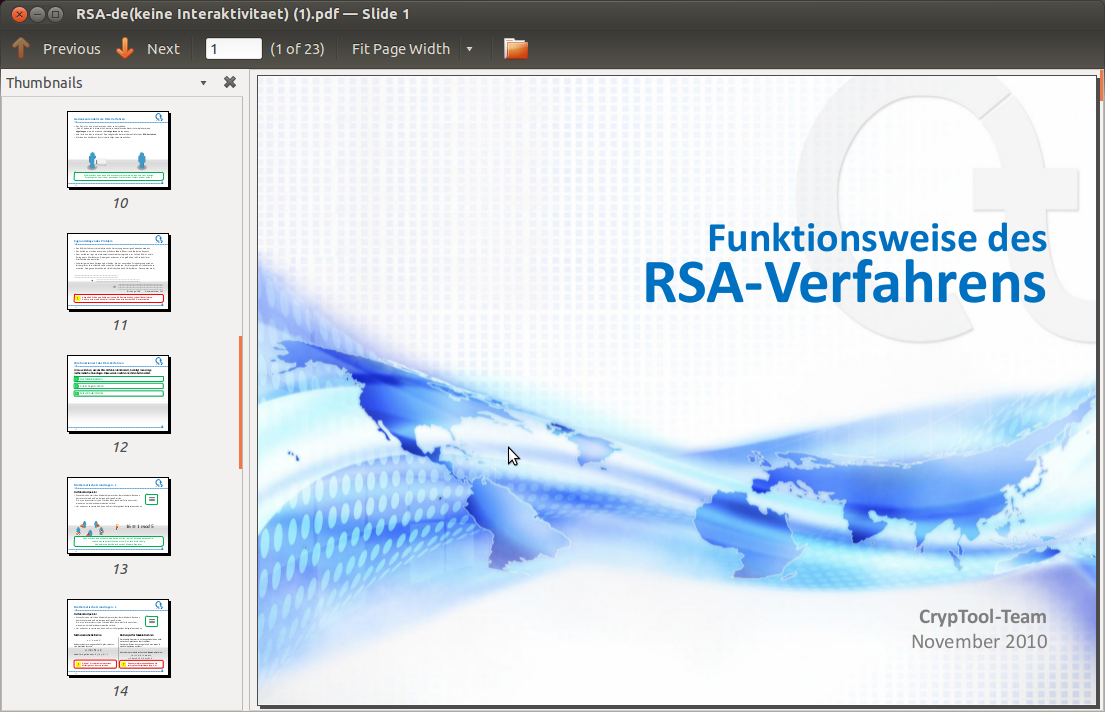
\includegraphics[scale=0.4]{figures/Interactive_RSA_Presentation_D.png}
\caption{Screenshot RSA-Pr�sentation (PDF)} 
\label{l_Interactive_RSA_Presentation}
\end{center}
\end{figure}



% ++++++++++++++++++++++++++++++++++++++++++++++++++++++++++++++++++++++++++
\newpage
\hypertarget{NumberTheory_Appendix_E}{}
\section{Anhang: Beispiele mit SageMath}
\label{NumberTheory_Appendix_E}{}
\index{SageMath}
\index{SageMath!Programmbeispiele}

\begin{ctsquote}
\glqq Nie w�rde sie ihren Eltern ... von dieser ganzen Welt erz�hlen k�nnen. Nicht von ihrer Arbeit, die im Knacken von Codes bestand. Nicht vom Fiasko der Daemon-Taskforce ... Nicht von den schattenhaften Marionetten, die die Regierung nach ihrer Pfeife tanzen lie�en.\grqq 
\caption[Daniel Suarez]{Daniel Suarez\footnotemark}\index{Suarez, Daniel}
\end{ctsquote}
\addtocounter{footnote}{0}\footnotetext{Daniel Suarez, \glqq Darknet\grqq,
     rororo, (c) 2011, Kapitel 19, \glqq Scheideweg\grqq, S. 229, Philips.}


\noindent In diesem Anhang finden Sie SageMath-Quellcode, mit dem Sie die Tabellen und
Beispiele des Kapitels~\ref{Chapter_ElementaryNT}
(\glqq \nameref{Chapter_ElementaryNT}\grqq) berechnen k�nnen. 


% ---------------------------------------------------------------------------
\hypertarget{nt:AppArith1}{}
\subsection{Multiplikationstabellen modulo m} 
\label{nt:AppArith1}{}

Die Multiplikationstabelle~\ref{mulmod17} (von Seite \pageref{SrcArith1a})
f�r $a \times i \pmod{m}$, mit $m = 17$, $a=5$ and $a=6$, und $i$ von $0$ bis $16$
kann mit folgenden SageMath-Befehlen berechnet werden:

\begin{sagecode}
\begin{Verbatim}%
[fontsize=\footnotesize]
sage: m = 17; a = 5; b = 6
sage: [mod(a * i, m).lift() for i in xrange(m)]
[0, 5, 10, 15, 3, 8, 13, 1, 6, 11, 16, 4, 9, 14, 2, 7, 12]
sage: [mod(b * i, m).lift() for i in xrange(m)]
[0, 6, 12, 1, 7, 13, 2, 8, 14, 3, 9, 15, 4, 10, 16, 5, 11]
\end{Verbatim}
\caption{Multiplikationstabelle $a \times i \pmod{m}$ mit $m = 17$, $a=5$ and $a=6$}
\end{sagecode}

\noindent Die Funktion \verb!mod()! gibt das Objekt zur�ck, das die nat�rlichen
Zahlen modulo $m$ (in unserem Fall $m = 17$) repr�sentiert.
Aus dem {\tt Mod}-Objekt kann man die einzelnen Komponenten entweder mit der
\texttt{component}- oder mit der \texttt{lift}-Funktion zur�ckgewinnen.
Wir nutzen hier die Methode \verb!lift()!, um das Objekt in eine Zahl umzuwandeln und
auszugeben.

Die weiteren Beispiele der Multiplikationstabelle modulo $13$ (Tabelle~\ref{mulmod13})
und modulo $12$ (Tabelle~\ref{mulmod12}) auf Seite \pageref{SrcArith1b}
kann man auf dieselbe Weise bestimmen, wenn man im Quelltext jeweils
{\tt m=17} durch den entsprechenden Zahlenwert ({\tt m=13} bzw. {\tt m=12}) ersetzt.


% ---------------------------------------------------------------------------
\vskip +25 pt
\hypertarget{nt:AppArith2}{}
\subsection{Schnelles Berechnen hoher Potenzen}
\label{nt:AppArith2}{}

Das schnelle Potenzieren modulo $m$ kann mit der SageMath-Funktion \verb!power_mod()!
durchgef�hrt werden. Das Ergebnis dieser Funktion ist eine nat�rliche Zahl.
Sie k�nnen mit Hilfe der folgenden Zeilen die Idee der Square-and-Multiply-Methode
nachvollziehen, wie sie im Beispiel in Kapitel \glqq \nameref{hohpot}\grqq~
auf Seite \pageref{SrcArith2} dargestellt ist:

\begin{sagecode}
\begin{Verbatim}%
[fontsize=\footnotesize]
sage: a = 87; m = 103
sage: exp = [2, 4, 8, 16, 32, 43]
sage: [power_mod(a, e, m) for e in exp]
[50, 28, 63, 55, 38, 85]
\end{Verbatim}
\caption{Schnelles Berechnen hoher Potenzen mod $m = 103$}
\end{sagecode}


% ---------------------------------------------------------------------------
\newpage
\hypertarget{nt:AppArith3a1}{}
\subsection{Multiplikative Ordnung}
\label{nt:AppArith3a1}{}

Die Ordnung $ord_m(a)$ einer Zahl $a$ in der multiplikativen Gruppe $Z_m^*$ ist
die kleinste nat�rliche Zahl $i \ge 1$ f�r die gilt $a^i \equiv 1$ mod $m$
(siehe Kapitel~\ref{MultOrdPrimitveRoot}, \glqq \nameref{MultOrdPrimitveRoot}\grqq).

Um die Tabelle~\ref{expmod11} auf Seite~\pageref{SrcArith3a} zu berechnen,
k�nnen wir alle Potenzen $a^i \pmod{11}$ wie folgt ausgeben:

\begin{sagecode}
\begin{Verbatim}%
[fontsize=\footnotesize]
sage: m = 11
sage: for a in xrange(1, m):
....:     print [power_mod(a, i, m) for i in xrange(1, m)]
....:
[1, 1, 1, 1, 1, 1, 1, 1, 1, 1]
[2, 4, 8, 5, 10, 9, 7, 3, 6, 1]
[3, 9, 5, 4, 1, 3, 9, 5, 4, 1]
[4, 5, 9, 3, 1, 4, 5, 9, 3, 1]
[5, 3, 4, 9, 1, 5, 3, 4, 9, 1]
[6, 3, 7, 9, 10, 5, 8, 4, 2, 1]
[7, 5, 2, 3, 10, 4, 6, 9, 8, 1]
[8, 9, 6, 4, 10, 3, 2, 5, 7, 1]
[9, 4, 3, 5, 1, 9, 4, 3, 5, 1]
[10, 1, 10, 1, 10, 1, 10, 1, 10, 1]

und die letzte Spalte erg�nzt um die Ordnung des jeweiligen a mod (11)

sage: m = 11
sage: for a in xrange(1, m):
....:     lst= [power_mod(a, i, m) for i in xrange(1, m)]
....:     lst.append(multiplicative_order(mod(a,m)))
....:     print lst
....:
[1, 1, 1, 1, 1, 1, 1, 1, 1, 1, 1]
[2, 4, 8, 5, 10, 9, 7, 3, 6, 1, 10]
[3, 9, 5, 4, 1, 3, 9, 5, 4, 1, 5]
[4, 5, 9, 3, 1, 4, 5, 9, 3, 1, 5]
[5, 3, 4, 9, 1, 5, 3, 4, 9, 1, 5]
[6, 3, 7, 9, 10, 5, 8, 4, 2, 1, 10]
[7, 5, 2, 3, 10, 4, 6, 9, 8, 1, 10]
[8, 9, 6, 4, 10, 3, 2, 5, 7, 1, 10]
[9, 4, 3, 5, 1, 9, 4, 3, 5, 1, 5]
[10, 1, 10, 1, 10, 1, 10, 1, 10, 1, 2]
\end{Verbatim}
\caption{Tabelle mit allen Potenzen $a^i \pmod{m}$ f�r $m=11$, $a=1,...,10$}
\label{nt_Sage-code_MultOrder_expmod11}%Creates table with label expmod11
\end{sagecode}


\newpage
\hypertarget{nt:AppArith3b}{}
\label{nt:AppArith3b}{}
Die Tabelle~\ref{expmod45} auf Seite~\pageref{SrcArith3b} enth�lt Beispiele
f�r die Ordnung von a modulo 45 ($ord_{45}(a)$) und den Wert der Eulerfunktion
von 45 ($J(45)$).

Der folgende SageMath-Code erzeugt eine analoge Tabelle.

\begin{sagecode}
\begin{Verbatim}%
[fontsize=\footnotesize]
sage: m = 45
sage: for a in xrange(1, 13):
....:     lst = [power_mod(a, i, m) for i in xrange(1, 13)]
....:     try:
....:         lst.append(multiplicative_order(mod(a, m)))
....:     except:
....:         lst.append("None")
....:     lst.append(euler_phi(m))
....:     print lst
....:
[1, 1, 1, 1, 1, 1, 1, 1, 1, 1, 1, 1, 1, 24]
[2, 4, 8, 16, 32, 19, 38, 31, 17, 34, 23, 1, 12, 24]
[3, 9, 27, 36, 18, 9, 27, 36, 18, 9, 27, 36, 'None', 24]
[4, 16, 19, 31, 34, 1, 4, 16, 19, 31, 34, 1, 6, 24]
[5, 25, 35, 40, 20, 10, 5, 25, 35, 40, 20, 10, 'None', 24]
[6, 36, 36, 36, 36, 36, 36, 36, 36, 36, 36, 36, 'None', 24]
[7, 4, 28, 16, 22, 19, 43, 31, 37, 34, 13, 1, 12, 24]
[8, 19, 17, 1, 8, 19, 17, 1, 8, 19, 17, 1, 4, 24]
[9, 36, 9, 36, 9, 36, 9, 36, 9, 36, 9, 36, 'None', 24]
[10, 10, 10, 10, 10, 10, 10, 10, 10, 10, 10, 10, 'None', 24]
[11, 31, 26, 16, 41, 1, 11, 31, 26, 16, 41, 1, 6, 24]
[12, 9, 18, 36, 27, 9, 18, 36, 27, 9, 18, 36, 'None', 24]
\end{Verbatim}
\caption{Tabelle mit allen Potenzen $a^i \pmod{45}$ f�r $a=1,...,12$ plus der Ordnung von a}
\label{nt_Sage-code_MultOrder_expmod45}
\end{sagecode}

Die Ordnung $\text{ord}_m(a)$ kann nur berechnet werden, wenn $a$
teilerfremd\index{Zahlen!teilerfremde (co-prime)} zu $m$ ist.
Das kann mit der Abfrage, ob \verb!gcd(a, m)==1!, �berpr�ft werden.

In unserem Codebeispiel haben wir stattdessen die Berechung der
multiplikativen Ordnung in einem \verb!try!-\verb!except!-Block
durchgef�hrt. Auf diese Weise kann SageMath jede Ausnahme und jeden Fehler
abfangen, der von der Funktion \verb!multiplicative_order()! geworfen wird.
Wird eine Ausnahmen oder ein Fehler im \verb!try!-Block geworfen, wissen
wir, dass $\text{ord}_m(a)$ nicht existiert f�r den gegebenen Wert von $a$.
Daher wird dann im \verb!except!-Block ans Ende der Zeile der String \verb!"None"!
angeh�ngt (die Zeile wird durch das Objekt \verb!lst! repr�sentiert).


\newpage
\hypertarget{nt:AppArith3c}{}
\label{nt:AppArith3c}{}
Die Tabelle~\ref{expmod46} auf Seite~\pageref{SrcArith3c} enth�lt Beispiele
f�r die Exponentiationen $a^i$ mod $46$ sowie die Ordnungen $ord_{46}(a)$ 

Der folgende SageMath-Code erzeugt eine analoge Tabelle.

\begin{sagecode}
\begin{Verbatim}%
[fontsize=\footnotesize]
sage: m = 46
sage: euler_phi(m)
22
sage: for a in xrange(1, 24):
....:     lst = [power_mod(a, i, m) for i in xrange(1, 24)]
....:     try:
....:         lst.append(multiplicative_order(mod(a, m)))
....:     except:
....:         lst.append("None")
....:     print lst
....:
[1, 1, 1, 1, 1, 1, 1, 1, 1, 1, 1, 1, 1, 1, 1, 1, 1, 1, 1, 1, 1, 1, 1, 1]
[2, 4, 8, 16, 32, 18, 36, 26, 6, 12, 24, 2, 4, 8, 16, 32, 18, 36, 26, 6, 12, 24, 2, 'None']
[3, 9, 27, 35, 13, 39, 25, 29, 41, 31, 1, 3, 9, 27, 35, 13, 39, 25, 29, 41, 31, 1, 3, 11]
[4, 16, 18, 26, 12, 2, 8, 32, 36, 6, 24, 4, 16, 18, 26, 12, 2, 8, 32, 36, 6, 24, 4, 'None']
[5, 25, 33, 27, 43, 31, 17, 39, 11, 9, 45, 41, 21, 13, 19, 3, 15, 29, 7, 35, 37, 1, 5, 22]
[6, 36, 32, 8, 2, 12, 26, 18, 16, 4, 24, 6, 36, 32, 8, 2, 12, 26, 18, 16, 4, 24, 6, 'None']
[7, 3, 21, 9, 17, 27, 5, 35, 15, 13, 45, 39, 43, 25, 37, 29, 19, 41, 11, 31, 33, 1, 7, 22]
[8, 18, 6, 2, 16, 36, 12, 4, 32, 26, 24, 8, 18, 6, 2, 16, 36, 12, 4, 32, 26, 24, 8, 'None']
[9, 35, 39, 29, 31, 3, 27, 13, 25, 41, 1, 9, 35, 39, 29, 31, 3, 27, 13, 25, 41, 1, 9, 11]
[10, 8, 34, 18, 42, 6, 14, 2, 20, 16, 22, 36, 38, 12, 28, 4, 40, 32, 44, 26, 30, 24, 10, 'None']
[11, 29, 43, 13, 5, 9, 7, 31, 19, 25, 45, 35, 17, 3, 33, 41, 37, 39, 15, 27, 21, 1, 11, 22]
[12, 6, 26, 36, 18, 32, 16, 8, 4, 2, 24, 12, 6, 26, 36, 18, 32, 16, 8, 4, 2, 24, 12, 'None']
[13, 31, 35, 41, 27, 29, 9, 25, 3, 39, 1, 13, 31, 35, 41, 27, 29, 9, 25, 3, 39, 1, 13, 11]
[14, 12, 30, 6, 38, 26, 42, 36, 44, 18, 22, 32, 34, 16, 40, 8, 20, 4, 10, 2, 28, 24, 14, 'None']
[15, 41, 17, 25, 7, 13, 11, 27, 37, 3, 45, 31, 5, 29, 21, 39, 33, 35, 19, 9, 43, 1, 15, 22]
[16, 26, 2, 32, 6, 4, 18, 12, 8, 36, 24, 16, 26, 2, 32, 6, 4, 18, 12, 8, 36, 24, 16, 'None']
[17, 13, 37, 31, 21, 35, 43, 41, 7, 27, 45, 29, 33, 9, 15, 25, 11, 3, 5, 39, 19, 1, 17, 22]
[18, 2, 36, 4, 26, 8, 6, 16, 12, 32, 24, 18, 2, 36, 4, 26, 8, 6, 16, 12, 32, 24, 18, 'None']
[19, 39, 5, 3, 11, 25, 15, 9, 33, 29, 45, 27, 7, 41, 43, 35, 21, 31, 37, 13, 17, 1, 19, 22]
[20, 32, 42, 12, 10, 16, 44, 6, 28, 8, 22, 26, 14, 4, 34, 36, 30, 2, 40, 18, 38, 24, 20, 'None']
[21, 27, 15, 39, 37, 41, 33, 3, 17, 35, 45, 25, 19, 31, 7, 9, 5, 13, 43, 29, 11, 1, 21, 22]
[22, 24, 22, 24, 22, 24, 22, 24, 22, 24, 22, 24, 22, 24, 22, 24, 22, 24, 22, 24, 22, 24, 22, 'None']
[23, 23, 23, 23, 23, 23, 23, 23, 23, 23, 23, 23, 23, 23, 23, 23, 23, 23, 23, 23, 23, 23, 23, 'None']
\end{Verbatim}
\caption{Tabelle mit allen Potenzen $a^i \pmod{46}$ f�r $a=1,...,23$ plus die Ordnung von a}
\label{nt_Sage-code_MultOrder_expmod46}
\end{sagecode}




\newpage
\hypertarget{nt:AppArith3d}{}
\label{nt:AppArith3d}{}
Der folgende Code f�r die Tabellen~\ref{expmod14} und~\ref{expmod22}
auf Seite~\pageref{expmod14} f. gibt auch gleich das Ergebnis so aus,
dass man es leicht in LaTeX weiter verarbeiten kann. Voraussetzung daf�r ist,
dass alle Inhalte vorher einem SageMath-Objekt (hier einer Matrix) zugewiesen
werden.\footnote{%
        Anmerkungen zu dem SageMath-Programm, insbesondere den
        SageMath-Indizes\index{SageMath}\index{SageMath!latex()}:
        \begin{compactitem}
         \item for x in xrange(2, 5) liefert 2,3,4.
         \item m = matrix(ZZ, 2, 5) hat 2 Zeilen und 5 Spalten.\\
               Die Zellen haben die Bezeichner m(0,0) bis m(1,4).
         \item Alle Elemente der Matrix m�ssen numerisch sein, daher \glqq 0\grqq
               statt \glqq None\grqq.
         \item Die Ausgabe von Matrizen kann man in SageMath so steuern:
\begin{Verbatim}
               sage: from sage.matrix.matrix0 import set_max_cols, set_max_rows
               sage: set_max_cols(100)
               sage: set_max_rows(100)
\end{Verbatim}
         \item Die Zyklusl�nge in der letzten Spalte in den
               Tabellen~\ref{expmod14} und~\ref{expmod22}
               wurde noch von Hand ermittelt.
        \end{compactitem}
        \vspace{-\baselineskip} % Hier n�tig, damit alles auf 1 Seite passt!
        }

\begin{sagecode}
\begin{Verbatim}%
[fontsize=\footnotesize]
def power_mod_order_matrix(m, max_a, max_i):
    r = matrix(ZZ, max_a+1, max_i+3)
    for a in xrange(0, max_a+1):
        r[a, 0] = a
        for i in xrange(1, max_i+1):
            if a==0:
                r[a,i] = i
            else:
                r[a, i] = power_mod(a, i, m)
        try:
            r[a, max_i+1] = multiplicative_order(mod(a, m))
        except:
            r[a, max_i+1] = 0
        r[a, max_i+2] = euler_phi(m)
    return r

print "\n1: m=45;max_i=13;max_a=13";m=45;max_i=13;max_a=13
r = power_mod_order_matrix(m, max_a, max_i);print r;print latex(r)

print "\n2: m=46;max_i=25;max_a=25";m=46;max_i=25;max_a=25
r = power_mod_order_matrix(m, max_a, max_i);print r.str();print latex(r)

print "\n3: m=14;max_i=13;max_a=16";m=14;max_i=13;max_a=16
r = power_mod_order_matrix(m, max_a, max_i);print r;print latex(r)

print "\n4: m=22;max_i=21;max_a=25";m=22;max_i=21;max_a=25
r = power_mod_order_matrix(m, max_a, max_i);print r.str();print latex(r)
...
3: m=14;max_i=13;max_a=16
[ 0  1  2  3  4  5  6  7  8  9 10 11 12 13  0  6]
[ 1  1  1  1  1  1  1  1  1  1  1  1  1  1  1  6]
[ 2  2  4  8  2  4  8  2  4  8  2  4  8  2  0  6]
[ 3  3  9 13 11  5  1  3  9 13 11  5  1  3  6  6]
...
\left(\begin{array}{rrrrrrrrrrrrrrrr}
0 & 1 & 2 & 3 & 4 & 5 & 6 & 7 & 8 & 9 & 10 & 11 & 12 & 13 & 0 & 6 \\
1 & 1 & 1 & 1 & 1 & 1 & 1 & 1 & 1 & 1 & 1 & 1 & 1 & 1 & 1 & 6 \\
2 & 2 & 4 & 8 & 2 & 4 & 8 & 2 & 4 & 8 & 2 & 4 & 8 & 2 & 0 & 6 \\
3 & 3 & 9 & 13 & 11 & 5 & 1 & 3 & 9 & 13 & 11 & 5 & 1 & 3 & 6 & 6 \\
...
\end{Verbatim}
\caption{Code f�r Tabellen mit allen Potenzen $a^i \pmod{m}$ f�r variable $a$ und $i$ plus Ordnung von a und Eulerphi von m}
\end{sagecode}




% ---------------------------------------------------------------------------
\newpage
\hypertarget{nt:AppArith3a2}{}
\subsection{Primitivwurzeln}
\label{nt:AppArith3a2}
\label{primitive-roots-with-sage}
\index{Primitivwurzel}

Das Berechnen von Primitivwurzeln
(siehe Kapitel~\ref{MultOrdPrimitveRoot}, \glqq \nameref{MultOrdPrimitveRoot}\grqq)
geht in SageMath sehr einfach: Sei \verb!n! eine nat�rliche Zahl, dann kann mit dem Befehl
\verb!primitive_root(n)! \textit{eine} Primitivwurzel der multiplikativen Gruppe
$(\mathbf{Z} / n \mathbf{Z})^{\ast}$ berechnet werden, sofern eine existiert.
Ist $n$ prim, dann ist das �quivalent zum Berechnen einer Primitivwurzel in
$\mathbf{Z} / n \mathbf{Z}$.

\noindent Im folgenden berechnen wir die Primitivwurzeln einiger nat�rlicher Zahlen.

\begin{sagecode}
\begin{Verbatim}%
[fontsize=\footnotesize]
sage: primitive_root(4)
3
sage: primitive_root(22)
13
sage: for p in primes(1, 50):
....:     print p, primitive_root(p)
....:     
2 1
3 2
5 2
7 3
11 2
13 2
17 3
19 2
23 5
29 2
31 3
37 2
41 6
43 3
47 5
\end{Verbatim}
\caption{Berechnen einer Primitivwurzel f�r eine gegebene Primzahl}
\end{sagecode}

\noindent Ist $p$ prim, dann hat $\mathbf{Z} / p \mathbf{Z}$ mindestens eine Primitivwurzel.\\



%\newpage
\noindent Will man \texttt{alle} Primitivwurzeln von $(\mathbf{Z} / n \mathbf{Z})^{\ast}$
berechnen, und nicht nur irgend eine einzige von $(\mathbf{Z} / n \mathbf{Z})^{\ast}$,
dann kann man das mit der folgenden selbstgeschriebenen Funktion durchf�hren%
\footnote{Der folgende Code wurde als SageMath-Skriptdatei erstellt und
nicht-interaktiv ausgef�hrt. Deshalb gibt es in der Ausgabe keine Zeilen,
die mit \glqq sage:\grqq~oder
\glqq ....:\grqq~anfangen wie in den SageMath-Programmbeispielen bisher.}.

\newpage %BERM_Warning: Egal, ob Newpage hier oder vor dem Text (wie im Englischen), warum gibt
         %              es nur im Deutschen die Warnung: "Text page 202 contains only floats."

\begin{sagecode}
\begin{Verbatim}%
[fontsize=\footnotesize]
def enum_PrimitiveRoots_of_an_Integer(M):
    r"""
    Return all the primitive roots of the integer M (if possible).
    """
    try:
        g = primitive_root(M)
    except:
        return None
    targetOrder = euler_phi(M)
    L=[]
    # Stepping through all odd integers from 1 up to M, not including
    # M. So this loop only considers values of i where 1 <= i < M.
    for i in xrange(1,M,2):
            testGen = Mod(g^i,M)
            if testGen.multiplicative_order() == targetOrder:
                L.append(testGen.lift())
    # removing duplicates
    return Set(L)

# AA_Start -- Testcases for enum_PrimitiveRoots_of_an_Integer(M)
print "AA_Start -- Testcases for enum_PrimitiveRoots_of_an_Integer(M)"
M=10; print "1-----------Testcase: M = %s" % M
LL = enum_PrimitiveRoots_of_an_Integer(M)
if LL==None:
    print M
else:
    print LL
M=8; print "2-----------Testcase: M = %s" % M
# M=8 hat keine primitive root mod m. Checke, ob per try - except abgefangen.
LL = enum_PrimitiveRoots_of_an_Integer(M)
if LL==None:
    print M
else:
    print LL
M=17; print "3-----------Testcase: M = %s" % M
LL = enum_PrimitiveRoots_of_an_Integer(M)
if LL==None:
    print M
else:
    print LL
# AA_End -- Testcases

OUTPUT:
AA_Start -- Testcases for enum_PrimitiveRoots_of_an_Integer(M)
1-----------Testcase: M = 10
{3, 7}
2-----------Testcase: M = 8
8
3-----------Testcase: M = 17
{3, 5, 6, 7, 10, 11, 12, 14}
\end{Verbatim}
\caption{Funktion \glqq enum\_PrimitiveRoots\_of\_an\_Integer\grqq~zur Berechnung
         aller Primitiv\-wurzeln f�r eine gegebene Zahl}
\end{sagecode}



\newpage
\noindent Das folgende Beispiel listet alle Primitivwurzeln der Primzahl 541 auf.

\begin{sagecode}
\begin{Verbatim}%
[fontsize=\footnotesize]
sage: L=enum_PrimitiveRoots_of_an_Integer(541); L
{2, 517, 10, 523, 13, 14, 527, 528, 18, 531, 24, 539, 30, 37, 40, 51,
54, 55, 59, 62, 65, 67, 68, 72, 73, 77, 83, 86, 87, 91, 94, 96, 98,
99, 107, 113, 114, 116, 117, 126, 127, 128, 131, 132, 138, 150, 152,
153, 156, 158, 163, 176, 181, 183, 184, 195, 197, 199, 206, 208,
210, 213, 218, 220, 223, 224, 244, 248, 250, 257, 258, 259, 260,
261, 263, 267, 269, 270, 271, 272, 274, 278, 280, 281, 282, 283,
284, 291, 293, 297, 317, 318, 321, 323, 328, 331, 333, 335, 342,
344, 346, 357, 358, 360, 365, 378, 383, 385, 388, 389, 391, 403,
409, 410, 413, 414, 415, 424, 425, 427, 428, 434, 442, 443, 445,
447, 450, 454, 455, 458, 464, 468, 469, 473, 474, 476, 479, 482,
486, 487, 490, 501, 504, 511}
sage: len(L)
144
\end{Verbatim}
\caption{Tabelle mit allen Primitivwurzeln der vorgegebenen Primzahl 541}
\end{sagecode}



\newpage
\noindent Mit etwas Programmieren kann man z�hlen, wie viele Primitivwurzeln
es gibt f�r alle nat�rlichen Zahlen in einem gegebenen Zahlenbereich.
Wir k�nnen das f�r alle Zahlen oder nur f�r die Primzahlen in diesem Bereich berechnen.

\begin{sagecode}
\begin{Verbatim}%
[fontsize=\footnotesize]
def count_PrimitiveRoots_of_an_IntegerRange(start, end, bPrimesOnly=True):
	r"""
	Compute all primitive roots of all numbers between start and end,
	inclusive, and count them.
	If the flag bPrimesOnly is True, it performs primality tests, so it
	allows us to count the number of primes from start to end, inclusive.
        If the flag bPrimesOnly is false, it additionally counts these even
	numbers which have no primitive root.
	"""
	nCheckedNumb = 0
	nCheckedNumb_WithoutPrimitivRoots = 0
	nPrimitiveRoots = 0
	for n in xrange(start, end+1):
		if bPrimesOnly:
			if is_prime(n):
				nCheckedNumb += 1
				L = enum_PrimitiveRoots_of_an_Integer(n)
				nPrimitiveRoots += len(L)
		else:
			nCheckedNumb += 1
			L = enum_PrimitiveRoots_of_an_Integer(n)
			if L==None:
				nCheckedNumb_WithoutPrimitivRoots += 1
			else:
				nPrimitiveRoots += len(L)

	if bPrimesOnly:
		print "Found all %s" % nPrimitiveRoots + \
		      " primitive roots of %s primes." % nCheckedNumb
	else:
		if nCheckedNumb_WithoutPrimitivRoots == 0:
			print "Found all %s " % nPrimitiveRoots + \
			      "primitive roots of %s numbers." % nCheckedNumb
		else:
			print "Found all %s " % nPrimitiveRoots + \
			      "primitive roots of %s numbers." % \
			          (nCheckedNumb - nCheckedNumb_WithoutPrimitivRoots)
			print "(Total of numbers checked: %s, " % nCheckedNumb + \
			      "Amount of numbers without primitive roots: %s)" % \
			          nCheckedNumb_WithoutPrimitivRoots
\end{Verbatim}
\caption{Funktion \glqq count\_PrimitiveRoots\_of\_an\_IntegerRange\grqq~zur Berechnung
         aller Pri\-mitivwurzeln f�r einen gegebenen Zahlenbereich}
\end{sagecode}


\newpage
\noindent Um zu sehen, wie lange unser Computer f�r diese Berechnung braucht,
kann man den SageMath-Befehl \verb!time! verwenden.

\begin{sagecode}
\begin{Verbatim}%
[fontsize=\footnotesize]
# BB_Start -- Testcases for count_PrimitiveRoots_of_an_IntegerRange(start, end, bPrimesOnly=True)
print "\n\nBB_Start -- Testcases for count_PrimitiveRoots_of_an_IntegerRange(start, end, True)"

print "\n1-----------Testcase: (1, 500)"
time count_PrimitiveRoots_of_an_IntegerRange(1, 500)

print "\n2-----------Testcase: (5, 6, False)"
time count_PrimitiveRoots_of_an_IntegerRange(5, 6, False)

print "\n3-----------Testcase: (1, 500, False)"
time count_PrimitiveRoots_of_an_IntegerRange(1, 500, False)
# BB_End -- Testcases

OUTPUT:
BB_Start -- Testcases for count_PrimitiveRoots_of_an_IntegerRange(start, end, bPrimesOnly=True)

1-----------Testcase: (1, 500)
Found all 8070 primitive roots of 95 primes.
Time: CPU 0.94 s, Wall: 0.97 s

2-----------Testcase: (5, 6, False)
Found all 3 primitive roots of 2 numbers.
Time: CPU 0.00 s, Wall: 0.00 s

3-----------Testcase: (1, 500, False)
Found all 11010 primitive roots of 170 numbers.
(Total of numbers checked: 500, Amount of numbers without primitive roots: 330)
Time: CPU 1.52 s, Wall: 1.59 s
\end{Verbatim}
\caption{Funktion \glqq count\_PrimitiveRoots\_of\_an\_IntegerRange\grqq: Testf�lle und Testausgaben}
\end{sagecode}




\clearpage
\noindent Mit unserer selbst erstellten Funktion \verb!enum_PrimitiveRoots_of_an_Integer!
kann man alle Primitivwurzeln einer Primzahl $p$ finden.

Die folgende Funktion z�hlt, wie viele Primitivwurzeln es innerhalb eines Primzahl-Bereiches
gibt, und gibt dann diese Primitivwurzeln jeweils aus.

Aus dieser Liste der Primitivwurzeln k�nnen wir jeweils die kleinste und gr��te
Primitivwurzel pro $\mathbf{Z} / p \mathbf{Z}$ bestimmen, als auch die Anzahl von
Primitivwurzeln pro $\mathbf{Z} / p \mathbf{Z}$ z�hlen.

\begin{sagecode}
\begin{Verbatim}%
[fontsize=\footnotesize]
def count_PrimitiveRoots_of_a_PrimesRange(start, end):
      r"""
      Compute all primitive roots of all primes between start and end,
      inclusive. This uses a primes iterator.
      """
      nPrimes = 0
      nPrimitiveRoots = 0
      for p in primes(start, end+1):
          L = enum_PrimitiveRoots_of_an_Integer(p)
	  print p, len(L)
          nPrimes += 1
          nPrimitiveRoots += len(L)
      print "Found all %s" % nPrimitiveRoots + " primitive roots of %s primes." % nPrimes

# CC_Start -- Testcases for count_PrimitiveRoots_of_a_PrimesRange(start, end)
print "\n\nBB_Start -- Testcases for count_PrimitiveRoots_of_a_PrimesRange(start, end)"
print "-----------Testcase: (1, 1500)"
time count_PrimitiveRoots_of_a_PrimesRange(1, 1500)
# CC_End -- Testcases

OUTPUT:
CC_Start -- Testcases for count_PrimitiveRoots_of_a_PrimesRange(start, end)
-----------Testcase: (1, 1500)
2 1
3 1
5 2
7 2
11 4
13 4
17 8
19 6
23 10
29 12
31 8
37 12
...
1483 432
1487 742
1489 480
1493 744
1499 636
Found all 62044 primitive roots of 239 primes.
Time: CPU 7.55 s, Wall: 7.85 s
\end{Verbatim}
\caption{Funktion \glqq count\_PrimitiveRoots\_of\_a\_PrimesRange\grqq~zur Berechnung
         aller Primitivwurzeln f�r ein gegebenes Intervall von Primzahlen}
\end{sagecode}



\newpage
\noindent Eine leicht ge�nderte Fassung unserer Funktion
\verb!count_PrimitiveRoots_of_a_PrimesRange! wurde nun benutzt, um eine
Liste (Datenbank) aller Primitivwurzeln f�r alle Primzahlen zwischen 1 und 100.000
zu erstellen.

\begin{sagecode}
\begin{Verbatim}%
[fontsize=\footnotesize]
start = 1
end = 10^5
fileName = "/scratch/mvngu/primroots.dat"
file = open(fileName, "w")
for p in primes(start, end+1):
    L = enum_PrimitiveRoots_of_an_Integer(p)
    print p, len(L)
    # Output to a file. The format is:
    # (1) the prime number p under consideration
    # (2) the number of primitive roots of Z/pZ
    # (3) all the primitive roots of Z/pZ
    file.write(str(p) + " " + str(len(L)) + " " + str(L) + "\n")
    file.flush()
file.close()
\end{Verbatim}
\caption{Code zur Erstellung einer Liste mit allen Primitivwurzeln f�r alle Primzahlen
         zwischen 1 und 100.000}
\end{sagecode}

Es dauerte rund einen ganzen Tag auf der Maschine sage.math, um die Datei
\glqq primroots.dat\grqq~zu erstellen (erstellt im Juli 2009 von Minh Van Nguyen xxxxxxxxxxx).

Auch dieser Code und die Funktion \verb!enum_PrimitiveRoots_of_an_Integer!
wurden in eine SageMath-Skriptdatei eingef�gt und nicht-interaktiv ausgef�hrt.

Die Datei \glqq primroots.dat\grqq~enth�lt die Liste alle Primitivwurzeln f�r alle
Primzahlen zwischen 1 und 100.000 inklusive. Dies ist eine sehr gro�e Datei
(ca. 1 GB unkomprimiert, ca. 285 MB komprimiert mit bzip2).
% Die Datei kann abgerufen werden unter
%   \url{http://sage.math.washington.edu/home/mvngu/doc/primitive-roots/primroots.dat.bz2}.
% Siehe auch Re: [sage-devel] what can we do with a database of primitive roots?
% https://groups.google.com/forum/m/#!topic/sage-devel/TA5Nk2GdhOI


\newpage
\noindent Diese Datei \glqq primroots.dat\grqq~wurde dann benutzt, um mit dem folgenden Code
drei Grafiken zu erstellen.

\begin{sagecode}
\begin{Verbatim}%
[fontsize=\footnotesize]
sage: # open a database file on primitive roots from 1 to 100,000
sage: file = open("/scratch/mvngu/primroots.dat", "r")
sage: plist = []    # list of all primes from 1 to 100,000
sage: nlist = []    # number of primitive roots modulo prime p
sage: minlist = []  # smallest primitive root modulo prime p
sage: maxlist = []  # largest primitive root modulo prime p
sage: for line in file:
....:     # get a line from the database file and tokenize it for processing
....:     line = line.strip().split(" ", 2)
....:     # extract the prime number p in question
....:     plist.append(Integer(line[0]))
....:     # extract the number of primitive roots modulo p
....:     nlist.append(Integer(line[1]))
....:     # extract the list of all primitive roots modulo p
....:     line = line[-1]
....:     line = line.replace("{", "")
....:     line = line.replace("}", "")
....:     line = line.split(", ")
....:     # sort the list in non-decreasing order
....:     line = [Integer(s) for s in line]
....:     line.sort()
....:     # get the smallest primitive root modulo p
....:     minlist.append(line[0])
....:     # get the largest primitive root modulo p
....:     maxlist.append(line[-1])
....:
sage: file.close()  # close the database file
sage: # plot of number of primitive roots modulo p
sage: nplot = point2d(zip(plist, nlist), pointsize=1)
sage: nplot.axes_labels(["x", "y"])
sage: nplot
sage: # plot of smallest primitive root modulo prime p
sage: minplot = point2d(zip(plist, minlist), pointsize=1)
sage: minplot.axes_labels(["x", "y"])
sage: minplot
sage: # plot of largest primitive root modulo prime p
sage: maxplot = point2d(zip(plist, maxlist), pointsize=1)
sage: maxplot.axes_labels(["x", "y"])
sage: maxplot
\end{Verbatim}
\caption{Code zur Erzeugung der Grafiken zur Verteilung der Primitivwurzeln}
\end{sagecode}




\newpage
Abbildung~\ref{fig:primitive_roots_all} gibt die Anzahl der Primitivwurzeln
f�r jede Primzahl zwischen 1 und 100.000 aus. Die $x$-Achse repr�sentiert
die Primzahlen 1 bis 100.000, die $y$-Achse gibt die Anzahl der Primitivwurzeln
pro Primzahl aus.

\begin{figure}[!htbp]
\centering
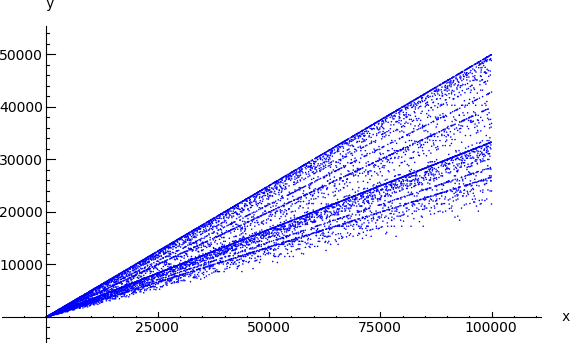
\includegraphics{figures/primitive-roots-all}
\caption{Die Anzahl der Primitivwurzeln f�r alle Primzahlen zwischen 1 und 100.000}
\label{fig:primitive_roots_all}
\end{figure}

\vskip +50 pt
Abbildung~\ref{fig:primitive_roots_smallest} gibt die kleinste Primitivwurzel
von jeder Primzahl zwischen 1 und 100.000 aus. Die $x$-Achse repr�sentiert
die Primzahlen 1 bis 100.000, die $y$-Achse gibt die kleinste Primitivwurzel
pro Primzahl aus.

\vskip +25 pt
Abbildung~\ref{fig:primitive_roots_largest} zeigt die entsprechende Graphik
mit der gr��ten Primitivwurzel zu jeder Primzahl im obigen Intervall.

\begin{figure}[!htbp]
\centering
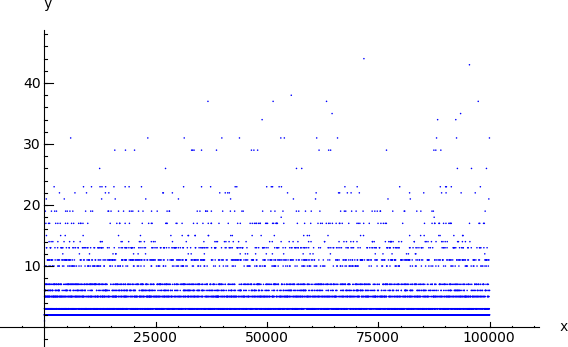
\includegraphics{figures/primitive-roots-smallest.png}
\caption{Die kleinste Primitivwurzel von jeder Primzahl zwischen 1 und 100.000}
\label{fig:primitive_roots_smallest}
\end{figure}

\begin{figure}[!htbp]
\centering
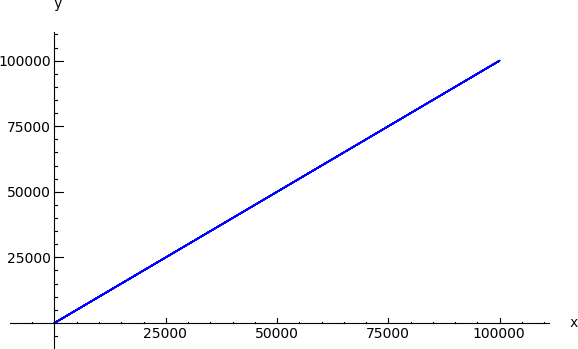
\includegraphics{figures/primitive-roots-largest.png}
\caption{Die gr��te Primitivwurzel von jeder Primzahl zwischen 1 und 100.000}
\label{fig:primitive_roots_largest}
\end{figure}

% To enforce that the next chapter starts at the beginning of a new page after
% the freely placed graphics, it was necessary to have TWO newpages and in between
% something to be printed (here invisible blanks).
% \newpage
% $ $
% I guess \clearpage is preferable.



% ---------------------------------------------------------------------------
\newpage
\hypertarget{NumberTheory_Sage_RSA_sample}{}
\subsection{RSA-Beispiele mit SageMath}
\label{l:NumberTheory_Sage_RSA_sample}{}

\noindent In diesem Abschnitt sind die SageMath-Quelltexte f�r die einfachen RSA-Beispiele
im Kapitel~\ref{rsaconcrete} (\glqq \nameref{rsaconcrete}\grqq) angegeben. 

\vskip +10 pt 
\hypertarget{nt:AppArith4a}{%
\noindent \textbf{Beispiel auf Seite~\pageref{SrcArith4a}:}}
\label{nt:AppArith4a}\\
Die RSA-Exponentiation $M^{37} \pmod{3713}$ f�r die Nachricht $M = 120$ kann
mit SageMath folgenderma�en ausgef�hrt werden:

\begin{Verbatim}%
[fontsize=\footnotesize]
sage: power_mod(120, 37, 3713)
1404
\end{Verbatim}


\vskip +10 pt 
\hypertarget{nt:AppArith4b}{%
\noindent {\bf Beispiel auf Seite~\pageref{SrcArith4b}:}}
\label{nt:AppArith4b}\\
Die Faktorisierung von $J(256.027) = 255.016 = 2^3 * 127 * 251$ kann mit SageMath
folgenderma�en durchgef�hrt werden:

\begin{sagecode}
\begin{Verbatim}%
[fontsize=\footnotesize]
sage: factor(255016)
2^3 * 127 * 251
\end{Verbatim}
\caption{Faktorisierung einer Zahl}
\end{sagecode}


\vskip +10 pt 
\hypertarget{nt:AppArith4c}{%
\noindent {\bf Beispiel auf Seite~\pageref{SrcArith4c}:}}
\label{nt:AppArith4c}\\
RSA-Verschl�sselung mit SageMath:

\begin{sagecode}
\begin{Verbatim}%
[fontsize=\footnotesize]
sage: A = [82, 83, 65, 32, 119, 111, 114, 107, 115, 33]
sage: e = 65537; m = 256027
sage: [power_mod(a, e, m) for a in A]
[212984, 25546, 104529, 31692, 248407, 100412, 54196, 100184, 58179, 227433]
\end{Verbatim}
\caption{RSA-Verschl�sselung durch modulare Exponentiation einer Zahl (als Nachricht)}
\end{sagecode}


\vskip +10 pt 
\hypertarget{nt:AppArith4d}{%
\noindent {\bf Beispiel auf Seite~\pageref{SrcArith4d}:}}
\label{nt:AppArith4d}\\
RSA-Verschl�sselung mit SageMath:

\begin{Verbatim}%
[fontsize=\footnotesize]
sage: A = [21075, 16672, 30575, 29291, 29473]
sage: e = 65537; m = 256027
sage: [power_mod(a, e, m) for a in A]
[158721, 137346, 37358, 240130, 112898]
\end{Verbatim}


\vskip +10 pt 
\hypertarget{nt:AppArith4e}{%
\noindent {\bf Beispiel auf Seite~\pageref{SrcArith4e}:}}
\label{nt:AppArith4e}\\
RSA-Verschl�sselung mit SageMath:

\begin{Verbatim}%
[fontsize=\footnotesize]
sage: A = [82083, 65032, 119111, 114107, 115033]
sage: e = 65537; m = 256027
sage: [power_mod(a, e, m) for a in A]
[198967, 51405, 254571, 115318, 14251]
\end{Verbatim}




% ---------------------------------------------------------------------------
\newpage
\hypertarget{NumberTheory_Sage_Number-of-RSA-keys}{}
%\subsection{Wie viele private RSA-Schl�ssel gibt es innerhalb eines Modulo-Bereiches?}
% \texorpdfstring{$d$}{d} not necessary as title-id and title-output separated.
% \subsection[Wie viele private RSA-Schl�ssel \texorpdfstring{$d$}{d} gibt es innerhalb eines Modulo-Bereiches?]
\subsection[Wie viele private RSA-Schl�ssel d gibt es innerhalb eines Modulo-Bereiches?]
{Wie viele private RSA-Schl�s\discretionary{-}{}{}sel $d$ gibt es innerhalb eines Modulo-Be\-rei\-ches?}

\label{l:NumberTheory_Sage_Number-of-RSA-keys}{}

Die RSA-Verschl�sselung wurde beschrieben in Abschnitt \ref{RSA} (\glqq \nameref{RSA}\grqq).
Schritt 1 bis 3 definieren die Schl�sselerzeugung, Schritt 4 und 5 stellen die
eigentliche Verschl�sselung dar:
\begin{itemize}
  \item[{\bf 1.}] W�hle zwei unterschiedliche Primzahlen $p$ and $q$
                  und berechne $n = p*q$.\\
                  Der Wert $n$ wird RSA-Modul genannt.

  \item[{\bf 2.}] W�hle ein zuf�lliges $e \in \{2, \cdots, n-1\}$, so dass gilt: \\
                  $e$ ist relativ prim
                  \index{Primzahl!relative}\index{Zahlen!relativ prim}
                  zu $J(n) = (p-1)*(q-1)$. \\
                  Danach kann man $p$ und $q$ \glqq wegwerfen\grqq.

  \item[{\bf 3.}] W�hle $d \in \{1, \cdots, n-1\}$ mit $e*d \equiv 1  
                  {\rm ~(mod~} J(n))$,\\
		  d.h. $d$ ist die multiplikative Inverse von $e$ modulo $J(n)$.
		  Dann kann man $J(n)$ \glqq wegwerfen\grqq.
    \begin{compactitem}
      \item[] $\rightarrow (n, e)$ ist der �ffentliche Schl�ssel $P$.
      \item[] $\rightarrow (n, d)$ ist der private Schl�ssel $S$ (nur $d$ muss man geheim halten).
    \end{compactitem}

  \item[{\bf 4.}] Zur Verschl�sselung wird die Nachricht als (bin�re) Ziffernfolge
                  geschrieben. Diese Ziffernfolge wird dann so in gleich lange
                  Teilfolgen aufgeteilt, dass jede Teilfolge eine Zahl kleiner als
                  $n$ darstellt.

  \item[{\bf 5.}] Vorgang der Verschl�sselung auf dem Klartext (bzw. auf Teilen davon)
                  $M \in \{1, \cdots, n-1\}$:
                  $$C = E ( (n, e); M ) := M^e {\rm ~(mod~} n).$$
\end{itemize}

Standardm��ig versucht man, einen mit RSA verschl�sselten Geheimtext $C$
dadurch zu knacken, dass man den �ffentlichen Schl�ssel des Empf�ngers
betrachtet und versucht, $n$ zu faktorisieren. Hat man das erreicht, geht man
wieder durch die Schritte 2 und 3 und erzeugt den privaten Schl�ssel $e$, den
man zum Entschl�sseln des Geheimtextes braucht.

Gem�� dem \glqq Primzahlsatz\grqq\footnote{%
Siehe Abschnitt \ref{thm-pz-pi-x} \glqq (\nameref{l_Primes_Distrib-of-Primes}\grqq).
% Der Ausdruck \nameref{thm-pz-pi-x}\grqq lieferte nur einen leeren String.
}
geht die Anzahl der Primzahlen $PI(x)$ asymptotisch gegen $x / ln(x)$.
Zwischen $1$ und einem gegebenen $n$ gibt es also ca. $n / ln(n)$ unterschiedliche
Primzahlen.

\noindent Will man nicht faktorisieren, sondern stellt sich eine Frage �hnlich
wie bei den klassischen Verschl�sselungsverfahren, kann man herausfinden wollen:
Wie viele verschiedene private Schl�ssel $(n, d)$ gibt es f�r einen bestimmten
Bereich der Schl�sselgr��e $n \in [a, b]$?\footnote{%
Kapitel~\ref{L_nt_Num-of-d-mod-26} (\glqq \nameref{L_nt_Num-of-d-mod-26}\grqq),
S.~\pageref{L_nt_Num-of-d-mod-26} behandelt den Spezialfall $n=26$.
}

\newpage
\noindent Das SageMath-Programm~\ref{nt_sagesample_Count_RSA_Keys} unten
definiert die Funktion \verb#count_Number_of_RSA_Keys#, die diese Frage konkret
beantwortet (wenn der Modulus nicht zu gro� ist).\footnote{%
%\begin{compactitem}
\newlength{\saveleftmargini}
\setlength{\saveleftmargini}{\leftmargini}
\setlength{\leftmargini}{0em}% for example to outdent verse
\settowidth{\versewidth}{xxxxx xxxxx xxxxx xxxxx xxxxx xxxxx xxxxx xxxxx xxxxx xxxxx xxxxx xxxxx xxxxx xxxxx xxxxx xxxxx xxxxx xxxxx}
\vspace{-\baselineskip} % TODO: Geht das nicht anders?
\begin{verse}[\versewidth]
 a) Der Aufruf \verb#sage: count_Number_of_RSA_Keys(100, 1000)# bedeutet, dass
man das Intervall $[100, 1000]$ f�r $n$ betrachtet.
$n$ war definiert durch die beiden Primzahlen $p, q: n = p*q$.
\verselinebreak Daher kann hier die eine Primzahl h�chstens den Wert $500$ annehmen, weil
$2 * 500 =1000$ (d.h. wenn die andere Primzahl den kleinst-m�glichen Primzahlwert $2$
annimmt).\\
\vin Die Anzahl m�glicher Primzahl-Kombinationen betr�gt: $comb = 258$.\\
\vin Die Anzahl der Primzahlen im gegebenen Bereich betr�gt: $143$.\\
\vin Die Anzahl der privaten Schl�ssel betr�gt: $34.816$.
\end{verse}
%\noindent %       \item
\begin{verse}[\versewidth]
 b) Der Aufruf \verb#sage: count_Number_of_RSA_Keys(100, 100, True)#
hat die folgende Ausgabe:\\
\vin    - Number of private keys for modulus in a given range: 0\\
\vin    - Number of primes in a given range: 0\\
\vin   Der Grund daf�r ist, dass mit diesem Aufruf nur $n=100$ betrachtet wird und
   die Funktion nur semiprime $n$\\ % TODO: Newline und anschlie�endes \vin sind nur Kr�cken,damit der ganze Satz vorne b�ndig! Unklar, wie man l�nger S�tze linksb�ndig ausgibt.
\vin untersucht. Die Zahl $100$ ist nicht
   semiprim\index{Primzahl!semiprime}\index{Primzahl!Halbprimzahl}\index{Halbprimzahl}\index{Zahlen!semiprime}, d.h. $100$ ist nicht das Produkt von genau zwei Primzahlen.
\end{verse}
\setlength{\leftmargini}{\saveleftmargini}% restore original value
%\end{compactitem}
}


\begin{sagecode}
\begin{Verbatim}%
[fontsize=\footnotesize]
def count_Number_of_RSA_Keys(start, end, Verbose=False):
      r"""
      How many private RSA keys (n,d) exist, if only modulus N is given, and start <= N <= end?
        (prime_range(u,o) delivers all primes >=u und < o).
      """
      a = start
      b = end
      s = 0
      comb = 0
      for p in prime_range(1, b/2+1):
          for q in prime_range(p + 1, b/2+1):
              if a <= p * q and p * q <= b:
                  comb = comb +1
                  s = s + (euler_phi(euler_phi(p * q))-1)
                  if Verbose:
                      print "p=%s, " % p + "q=%s, " % q + "s=%s" % s
      print "Number of private keys d for modulus in a given range: %s" % s + " (comb=%s), " % comb

      # Just for comparison: How many primes are in this range?
      s = 0
      for p in prime_range(a, b+1):
          if Verbose:
              print "a=%s, " % a + "b=%s, " % b + "p=%s" % p
          s = s + 1
      print "Number of primes in a given range: %s" % s

print "\n\nDD_Start -- Testcases for count_Number_of_RSA_Keys(start, end)"
print "\n-----------Testcase: (100, 1000) [Should deliver 34.816]"
time count_Number_of_RSA_Keys(100, 1000)
print "\n-----------Testcase: (100, 107, True) [Should deliver 23]"
time count_Number_of_RSA_Keys(100, 107, True)
u = 10^3; o = 10^4;
print "\n-----------Testcase: (%s, " % u + "%s) [Should deliver 3.260.044]" % o
time count_Number_of_RSA_Keys(u, o)

OUTPUT:
DD_Start -- Testcases for count_Number_of_RSA_Keys(start, end)

-----------Testcase: (100, 1000) [Should deliver 34.816]
Number of private keys d for modulus in a given range: 34816 (comb=258),
Number of primes in a given range: 143
Time: CPU 0.03 s, Wall: 0.04 s

-----------Testcase: (100, 107, True) [Should deliver 23]
p=2, q=53, s=23
Number of private keys d for modulus in a given range: 23 (comb=1),
a=100, b=107, p=101
a=100, b=107, p=103
a=100, b=107, p=107
Number of primes in a given range: 3
Time: CPU 0.00 s, Wall: 0.00 s

-----------Testcase: (1000, 10000) [Should deliver 3.260.044]
Number of private keys d for modulus in a given range: 3260044 (comb=2312),
Number of primes in a given range: 1061
Time: CPU 0.63 s, Wall: 0.66 s
\end{Verbatim}
\caption{Wie viele private RSA-Schl�ssel d gibt es, wenn man den Bereich f�r die Schl�ssel\-gr��e n kennt?}
\label{nt_sagesample_Count_RSA_Keys}
\end{sagecode}

\noindent Weil es mehr private Schl�ssel $(n, d)$ innerhalb eines gr��eren
Bereiches von Werten f�r $n$ gibt, ist das Brute-Force-Faktorisieren
viel effizienter als das Durchprobieren aller m�glichen Schl�ssel.




% ---------------------------------------------------------------------------
\clearpage
\newpage
\hypertarget{NumberTheory_Sage_Number-of-RSA-FixedPoints}{}
\subsection
    [RSA-Fixpunkte \texorpdfstring{}{m = m\^{}e}]%Das kommt ins Inhaltsverzeichnis
    {RSA-Fixpunkte $ m^e = m \bmod n $ mit $m \in \{1,...,n-1\}$ }
\label{l:NumberTheory_Sage_Number-of-RSA-FixedPoints}{}
\index{Fixpunkt}\index{RSA!Fixpunkt}
%%% xxx111222xxx-beg

Auch Verschl�sselungsverfahren k�nnen Fixpunkte haben, also Texte, deren Chiffrat
mit dem Original �bereinstimmt. In der Mathematik nennt man Variablen, die von einem
Verfahren (Funktion) auf sich selbst abgebildet werden, Fixpunkte. In der Kryptographie nennt man entsprechende Nachrichten "`unconcealed messages"' ("`unconcealed"' = unverborgen, offen). 

Generell gilt: Je mehr Fixpunkte ein Verschl�sselungsalgorithmus besitzt,
desto einfacher ist es, ihn zu knacken.

Beim RSA-Verfahren gilt: $n=pq$ ist das Produkt zweier verschiedener Primzahlen, und
es gibt ein $e$ mit $ggT(e,(p-1)(q-1))=1$. Die Verschl�sselung erfolgt mit
$c = m^e \mod n$. 
Ein Fixpunkt beim RSA-Verfahren ist eine Nachricht $m$, f�r die gilt:
$m = m^e \mod n$. Das Ergebnis der Verschl�sselung ist wieder die gegebene
Nachricht.

Die Wahrscheinlichkeit f�r das Auftreten von Fixpunkten ist bei RSA bei gen�gend
gro�em $n$ allerdings sehr gering -- wie Abbildung \ref{fig:NumberFixpointsGrowingN}
zeigt: Im Durchschnitt fanden wir nicht mehr als 40 Fixpunkte.

Studenten nehmen oft an, dass es viele Fixpunkte gibt, da sie beim Probieren mit
relativ \textbf{kleinen} Primzahlen immer auf "`relativ"' viele Fixpunkte-Beispiele
sto�en, denn m = 0, 1 und n-1 sind immer auch Fixpunkte.

In der Praxis, also bei gro� genug gew�hlten Primzahlen, haben Fixpunkte keine
Bedeutung f�r die Sicherheit von RSA. Deshalb bezieht sich dieser Abschnitt
eher auf mathematische Fragen.\footnote{%
Dank geht an Taras Shevchenko, der Teile des Inhalts dieses Abschnitts zusammentrug, und an Volker Simon, der das SageMath-Programm \ref{nt_sagesample_Calculate_RSA-Fixpoints}
\glqq Getfixpoints\grqq~% "`Getfixpoints"'
schrieb.}


% ----------------------------------------------------
\subsubsection{Die Anzahl der RSA-Fixpunkte}
In diesem Kapitel zeigen wir, wie viele RSA-Fixpunkte es f�r $m \in \{1,...,n-1\} $ gibt.\\

\begin{satz}\label{nt-number-of-fixpoints-1-to-n-1}
Die Anzahl der Fixpunkte $ m^e = m \bmod n$ mit $m \in \{1,...,n-1\} $ ist \\$ ggT(p-1, e-1) \cdot ggT(q-1, e-1) $.
\end{satz}
\begin{proof}
Sei $m^e = m \bmod n.$
Nach dem CRT\index{CRT}\footnote{%
CRT = Chinesischer Restsatz. 
\url{http://de.wikipedia.org/wiki/Chinesischer_Restsatz}
} sind die beiden folgenden Aussagen �quivalent:\\
$$ [ m^e = m \bmod n ]  \Leftrightarrow [ m^{e} = m \bmod p \text{  und  } m^{e} = m \bmod q ] $$
Diese Zerlegung ist �quivalent zu:
$$m^{e-1} = 1 \bmod p \text{  und  } m^{e-1} = 1 \bmod q. $$

\noindent Wir betrachten  $m^{e-1} = 1 \bmod p $ und  suchen alle $(e-1)$-ten
Einheitswurzeln\index{Einheitswurzel}\footnote{%
- In der Algebra werden Zahlen $x$, deren n-te Potenz die Zahl 1 ergibt, n-te \textbf{Einheitswurzeln} genannt.

\noindent- Eine $n$-te Einheitswurzel $x$ hei�t \textbf{primitiv}, falls f�r $x$ gilt:
 $$x^{n} = 1  \text{ und }   x^{k} \neq 1 ~~~(k = 1,2, 3, ..., n-1)$$

% Was ist der Zusammenhang zw. "Primitivwurzel" und "primitiver Einheitswurzel"?

\noindent- Ist $F$ ein endlicher K�rper und $n$ eine nat�rliche Zahl, dann ist eine
$n$-te Einheitswurzel in $F$ eine L�sung der Gleichung $$ x^{n}-1 = 0 \text{ in } F $$
}
in $\mathbb{Z}_p^{*}.$\\
Es gilt:~~ $\mathbb{Z}_p^{*}$ f�r p prim ist zyklisch.~~$\Rightarrow $~~
Es existiert ein Generator $g$, der $\mathbb{Z}_p^{*}$ erzeugt: $\mathbb{Z}_p^{*}=<g>$.

\noindent Der ff. Satz aus \cite[S. 69]{nt:Katzenbeisser2001}\index{Katzenbeisser 2001} charakterisiert alle $(e-1)$-ten Einheitswurzeln in $\mathbb{Z}_p^{*}$:
%\begin{lem}[$\cite{nt:Katzenbeisser2001}$]
%\end{lem}
\begin{satz}\label{nt-katzenbeisser-Anzahl-Einheitswurzeln}
$g^{\alpha}$ ist genau dann $(e-1)$-te Einheitswurzel in $\mathbb{Z}_p^{*}$,
wenn $(e-1)\alpha = 0\bmod p-1.$ Davon gibt es $ggT(p-1, e-1)$ viele.
\end{satz}
\begin{proof} 
Die erste Behauptung ergibt sich direkt aus dem kleinen Satz von Fermat:
\[g^{\alpha (e-1)}= 1 \bmod p  ~~\Rightarrow~~ \alpha (e-1) = 0\bmod p-1 \]
%%% Kann man diese �quivalenz zum Rechnen in den Exponenten mod (p-1) wirklich aus dem
%%% kleinen Satz von Fermat folgern:
%%%           a^p = a mod p  oder  a^(p-1)=1 mod p
 Sei $\delta =ggT(p-1, e-1)$. Aus $\alpha (e-1) = 0\bmod p-1$ folgt, dass $\frac{\alpha (e-1)}{\delta}= 0 \bmod \frac{p-1}{\delta}$. \\
Da $\frac {e-1}{\delta}$ und $\frac{p-1}{\delta}$ teilerfremd sind (da jeweils durch
den ggT ihrer Z�hler gek�rzt wurde), muss $\alpha$ ein Vielfaches von $\frac{p-1}{\delta}$ sein.

\[ \alpha \frac{p-1}{\delta} ~~ \text{mit} ~~ \alpha = 1,...,\delta
\]\\
Diese $\delta$ verschiedenen Potenzen entsprechen dann den 
$(e-1)$-ten Einheitswurzeln $g^{\alpha \frac{p-1}{\delta}} \bmod p$ in $\mathbb{Z}_p^{*}$.
\end{proof}
%%%% Ist $g^{\alpha \frac{p-1}{\delta}} \bmod p$ in $\mathbb{Z}_p^{*}$ richtig?

\noindent Analog f�r $q$: F�r $m^{e-1} = 1 \bmod q $ haben wir dann $ ggT(q-1, e-1) $ viele $(e-1)$-te Einheitswurzeln.\\

\noindent Die Anzahl der Arten, die $(e-1)$-ten Einheitswurzeln in $\mathbb{Z}_p^{*}$ und
$\mathbb{Z}_q^{*}$ zu kombinieren, ergibt die Gesamt-Anzahl der RSA-Fixpunkte
$ m^e = m \bmod n$ mit $ m \in \{1,...,n-1\}$:\\
 $ggT(p-1, e-1) \cdot ggT(q-1, e-1) $\\


\noindent Nimmt man $m=0$ hinzu, ergibt sich Satz \ref{nt-thm-Anzahl-RSA-Fixpunkte}:
\begin{satz}\label{nt-thm-Anzahl-RSA-Fixpunkte}
Wenn $ m \in \{0,...,n-1\}$ ist, dann ist die Anzahl der RSA-Fixpunkte:
          \[ (ggT(p-1, e-1)+1) \cdot (ggT(q-1, e-1)+1) \]
\end{satz}
\end{proof}
\vspace{15pt}



% ----------------------------------------------------
\subsubsection{Untere Schranke f�r die Anzahl der RSA-Fixpunkte}
Im folgenden Kapitel zeigen wir, dass eine untere Schranke f�r die Anzahl der RSA-Fixpunkte existiert. Diese untere Schranke $6$ liegt vor, wenn die beiden unterschiedlichen RSA-Primzahlen die kleinstm�glichen sind (2 und 3).\\

\noindent\textbf{Behauptung 1: $p = 2, q = 3$}\\
Die Anzahl der RSA-Fixpunkte f�r $p=2$ und $q=3$ ist\\
$(\underbrace{ggT(p-1, e-1)}_{=1}+1) \cdot (\underbrace{ggT(q-1, e-1)}_{=2}+1)=2 \cdot 3=6$ \\

\noindent\textbf{Behauptung 2: $p \neq q; p > 2,q > 2$}\\
Die Anzahl der RSA-Fixpunkte f�r $p \neq q; p,q > 2$ ist $\geq 9$.

\begin{proof}
Da $p$ und $q$ prim sind, sind $(p-1)$ und $(q-1)$ f�r $ p,q > 2 $ gerade.\\
Nach dem RSA-Verfahren ist e so zu w�hlen, dass $1 < e < \phi(n)=(p-1)(q-1)$ und \\
$ggT(e,(p-1)(q-1))=1$\\
Da $(p-1)$ und $(q-1)$ gerade sind, ist e ungerade $ \Rightarrow e-1$ ist gerade.\\
Da $(p-1)$ und $(e-1)$ gerade sind, gilt:\\
$ggT(p-1, e-1) \geq 2$ \\
$\Rightarrow (ggT(p-1, e-1)+1) \geq 3$ und $(ggT(q-1, e-1)+1) \geq 3$\\
$\Rightarrow (ggT(p-1, e-1)+1) \cdot (ggT(q-1, e-1)+1) \geq 9$
\end{proof}

\noindent Beispiele:\\
F�r $(e,n)=(17,6)$ sind alle sechs m�glichen Nachrichten \{0,1,2,3,4,5\} Fixpunkte (bei $n=6$ ist das unabh�ngig vom Wert von $e$).\\
F�r $(e,n)=(17,10)$ sind alle 10 m�glichen Nachrichten Fixpunkte.\\
F�r $(e,n)=(19,10)$ sind nur 6 der 10 m�glichen Nachrichten Fixpunkte. 



% ----------------------------------------------------
\vspace{15pt}
\subsubsection{Ungeschickte Wahl von \texorpdfstring{$e$}{e} }

In diesem Kapitel zeigen wir, dass mit $e=1+kgV(p-1,q-1)$ jede Verschl�sselung einen
Fixpunkt liefert (unabh�ngig von der Gr��e von p, q oder n); und erweitern das dann
auf alle m�glichen schlecht gew�hlten Werte f�r $e$.\\
%%% Wie viele solcher ungeschickter e existieren?
%%% Warum muss es das kgV sein, und kann nicht irgendein Vielfaches von phi? 

\noindent Wenn $e=1$, dann gilt f�r alle $ m$: $ c = m^e = m$. Das ist der Trivialfall.\\

\noindent\textbf{Behauptung 1: $p,q > 2$}\\
Wenn $e=1+kgV(p-1,q-1)$, dann gilt f�r alle $ m \in \{1,...,n-1\}$: $ m^e = m \bmod n$.

\begin{proof}~\\  % Erzwingen der Leerzeile nach "Beweis."
Es gilt:\\
-~~~ $ ~~~ e\cdot d=1 \mod \phi(n)$ ~oder~ $e\cdot d=1 \mod kgV(p-1,q-1) $\\
-~~~ $ ~~~ m^{x} \mod n = m^{x \mod \phi(n)} \mod n $\\

\noindent Verschl�sseln von Nachrichten: \\
 $~~~c=m^e \mod n$, wobei c der Geheimtext und m der Klartext ist.

\noindent Entschl�sseln von Nachrichten:\\
 $~~~m'=c^d \mod n$, wobei d die multiplikative Inverse von e ist.\\

\noindent Zu zeigen ist: $c=m \mod n$ f�r das gew�hlte e.

$~~~c = m^e \mod n$

$~~~c = m^{1+kgV(p-1,q-1)} \mod n$  ~~~~~\# Umformung gilt aufgrund der Voraussetzung

$~~~c = m^1 \cdot m^{k \cdot (p-1) \cdot (q-1)} \mod n$

$~~~c = m^1 \cdot m^{[k \cdot \phi(n)] \mod \phi(n)} \mod n$

$~~~c = m^1 \cdot m^{0} = m \mod n $
\end{proof}

\newpage
%~\\ % Zeilenumbruch erzwingen 
\noindent\textbf{Beispiel: Fixpunkteigenschaft f�r alle m:}\\
Gegeben sei $n=p\cdot q= 13\cdot 37=481\\
\Rightarrow \phi(n)=(p-1)(q-1)=12\cdot 36=432$\\
$\Rightarrow e=kgV(p-1,q-1)+1=kgV(12,36)+1=36+1=37$.\\
Mit $m \in \{4,6,7,480\}$ ergibt sich $m^{e} \mod n$ als:\\
$~~4^{37} \mod 481=~~4 $\\
$~~6^{37} \mod 481=~~6 $ \\
$~~7^{37} \mod 481=~~7 $ \\
$480^{37} \mod 481=480 $ \\


~\\ % Zeilenumbruch erzwingen
\noindent Es gibt nicht nur das einzige $e$ (siehe oben), so dass f�r alle $ m \in \{1,...,n-1\}$ die Fixpunkteigenschaft $ m^e = m \bmod n$ gilt.\footnote{%
  Man kann diese $e$, die jede Nachricht zu einem Fixpunkt machen, als
  "`schwache Schl�ssel"' $(e,n)$ des RSA-Verfahrens
  bezeichnen\index{Schl�ssel!schwach}.
  Diese Bezeichnung unterscheidet sich jedoch von den "`schwachen Schl�sseln"'
  $k$ bei DES\index{DES}, die \textbf{jede} Nachricht $m$ bei doppelt
  hintereinander durchgef�hrter \textbf{Ver}schl�sselung auf sich selbst
  abbilden.
  Das RSA-Verfahren kennt m.W. f�r gr��ere $n$ keine schwachen Schl�ssel
  dieser Art: $(m^e)^e = m$.\\
  In JCT\index{JCrypTool} findet man schwache DES-Schl�ssel in der
  Standard-Perspektive �ber den Men�eintrag {\bf Visualisierungen
  \textbackslash{} Innere Zust�nde im Data Encryption Standard (DES)}.
}

\begin{satz}\label{nt-thm-complete-fixed-point-property-values-of-e}
Die vollst�ndige Fixpunkteigenschaft aller $m$ gilt f�r jedes\\
$e=j\cdot kgV(p-1,q-1)+1$, wobei $j=0,1,2,3,4, ... $ bis $e \leq \phi(n)$.
\end{satz}

~\\ % Zeilenumbruch erzwingen 
\noindent\textbf{Beispiel: Weitere Werte f�r $e$ mit Fixpunkteigenschaft:}\\
Betrachten wir wieder
$n=p\cdot q= 13\cdot 37=481$ mit $kgV(p-1,q-1)=kgV(12,36)=36$.\\
Dann kann $e$ die ff. Werte annehmen: $e=j\cdot kgV(p-1,q-1)+1$ f�r $j=0,1,2,...,11$:\\
$\Rightarrow e \in \left\{ 1, 37,73,109,145,181,217, 253, 289, 325, 361,397\right\}$.\\

\noindent Ab $j=12$ gilt: $ e=12\cdot kgV(12,36)+1=432+1=433 > 432=\phi(n)$.\\

\noindent �berpr�fen wir z.B. wieder die obigen vier Werte f�r $m$ mit $e=217$, ergibt sich:\\
$~~4^{217} \mod 481=~~4 $\\
$~~6^{217} \mod 481=~~6 $ \\
$~~7^{217} \mod 481=~~7 $ \\
$480^{217} \mod 481=480 $ \\

\begin{satz}\label{nt-thm-complete-fixed-point-property-number-of-e}
Die Anzahl der m�glichen Werte f�r $e\text{ mit } m^e = m \bmod n$ l�sst sich wie folgt berechnen:
\[\left[ \text{Anzahl }e \right]=\left\lfloor \frac{\phi(n)}{kgV(p-1,q-1)+1}\right\rfloor +1=\frac{\phi(n)}{kgV(p-1,q-1)}
\]
\end{satz}

\noindent In unserem Beispiel ergibt dies $\frac{432}{kgV(12,36)}=12 $ verschiedene Werte
f�r $e$, bei denen f�r alle $m$ in $\mathbb{Z}_{481}$ gilt: $m^e = m \bmod n$.\\
~\\ % Zeilenumbruch erzwingen 



% ----------------------------------------------------
\newpage
\subsubsection[Empirische Absch�tzung der Anzahl der Fixpunkte f�r wachsende Moduli]{Eine empirische Absch�tzung der Anzahl der Fixpunkte f�r wachsende Moduli}
In diesem Kapitel machen wir eine empirische Absch�tzung der Anzahl der Fixpunkte
f�r wachsende Moduli (und nicht schwache $e$).

\noindent Dabei haben wir $p $ und $ q$ zuf�llig aus den sechs folgenden Bereichen
gew�hlt (jeder gkennzeichnet durch seine untere und obere Schranke):\\
$(2^2, 2^{10}), (2^{10}, 2^{20}), (2^{20}, 2^{40}), (2^{40}, 2^{80}),
 (2^{80}, 2^{160}), (2^{160}, 2^{320})$.\\
In jedem Bereich haben wir 10 Versuche gemacht. F�r den Exponenten $e$ haben wir
immer den Standardwert $e=2^{16}+1$ genommen. Die Anzahl der Fixpunkte wurde f�r
alle 60 Versuche mit dem Programm
\ref{nt_sagesample_Calculate_RSA-Fixpoints} "`Getfixpoints.sage"' berechnet.

\noindent Die folgenden f�nf Mengen enthalten die zuf�llig gew�hlten Wertepaare (p,q) innerhalb
der ersten f�nf Gr��enbereiche.

\begin{equation*}
  \begin{split}
Aus (2^2, 2^{10}): (p,q)~\in~ & \{ (127,947),(349,809),(47,461),(587,151),(19,23),\\ 
                              & (709,509),(653,11),(859,523),(823,811),(83,331)\} \\
\\
Aus (2^{10}, 2^{20}): (p,q)~\in~
            & \{ (447401,526283),(474223,973757),(100829,126757),(35803,116933),\\
            &    (577751,598783),(558121,607337),(950233,248167),(451103,73009),\\
            &    (235787,164429),(433267,287939)\} \\
  \end{split}
\end{equation*}

\begin{equation*}
  \begin{split}
Aus (2^{20},2^{40}): (p,q)~\in~
            & \{ (58569604997,321367332149),(286573447351,636576727223),\\
            &    (134703821971,134220414529),(161234614601,711682765579), \\
            &    (19367840881, 804790726361),(932891507377,521129503333),\\
            &    (337186437739,426034644493),(986529569219,604515928397),\\
            &    (276825557171,654134442649),(639276602353,1069979301731) \} \\
  \end{split}
\end{equation*}

\begin{equation*}
  \begin{split}
Aus (2^{40}, 2^{80}): (p,q)~\in~
            & \{ (667530919106151273090539,287940270633610590682889),\\
            &    (437090557112369481760661,590040807609821698387141),\\
            &    (1131921188937480863054851,813935599673320990215139)\\
            &    (874130181777177966406673,632270193935624953596331),\\
            &    (599303355925474677078809,717005631177936134003029),\\
            &    (752829320004631398659063,714134510643836818718761),\\
            &    (1046313315092743492917349,835721729660755006973833),\\
            &    (877161707568112212806617,42831503328261105793649),\\
            &    (575464819450637793425803, 5425832051159043433027),\\
            &    (321404337099945148592363,992663778486687980443879) \} \\
  \end{split}
\end{equation*}

\begin{equation*}
  \begin{split}
Aus (2^{80}, 2^{160}): (p,q)~\in~
   & \{ (838952969674957834783403492645269831354775774659,\\
   &     694309130163549038783972189350416942879771871411),\\
   &    (981985107290629501374187748859961786804311564643,\\
   &     178616495258601001174141825667078950281544628693),\\
   &    (614446632627716919862227545890890553330513965359,\\
   &     761232454374959264696945191327265643178491649141),\\
   &    (1421756952722008095585945863962560425554707936337,\\ 
   &     986781711714138924140285492105143175328486228197),\\
   &    (862346475785474165539441761205023498091366178341,\\ 
   &     438589995804600940885415547506719456975478582911),\\
   &    (1034081318899669345416602574034081247538053001533,\\
   &     1207032778571434704618111297072774884748706223447),\\
   &    (308083812465705343620096534684980088954958466893,\\ 
   &     350597371862294596793629011464584694618569736021),\\
   &    (830376326124356299120963861338027196931951857769,\\ 
   &     924874232653136669722297184352059466357375363191),\\
   &    (85600581120154590810189237569820706006659829231, \\
   &     297064381842806596646150718828138629443319259829),\\
   &    (1358984492013516052055790129324581847590275909129,\\
   &     609402294805414245544586792657989060761523960427) \} \\
  \end{split}
\end{equation*}


\begin{figure}[!htb]  %[htbp]
  \centering
   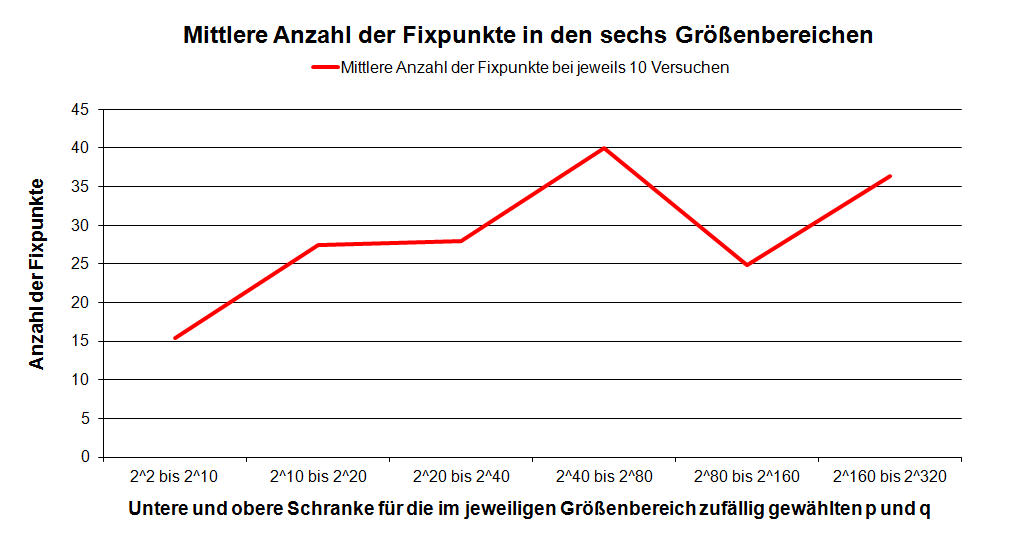
\includegraphics[width=0.92\textwidth]{figures/MAF.png}
  \caption{Eine empirische Absch�tzung der Anzahl der Fixpunkte f�r wachsende Moduli}
  \label{fig:NumberFixpointsGrowingN}
  %\vskip +45pt
\end{figure}

Abbildung \ref{fig:NumberFixpointsGrowingN} zeigt, dass innerhalb der sechs Gr��enbereiche die durchschnittliche Anzahl der Fixpunkte nicht gr��er als 40 ist.
% Leider konnten wir die Moduli in noch h�heren Bereichen nicht testen, da unser
% SageMath-Programm \ref{nt_sagesample_Calculate_RSA-Fixpoints}  "`Getfixpoints"'
% in Bereichen mit $(p,q) > 2^{320}$ zu langsam ist. \\



\vspace{15pt}
% ----------------------------------------------------
\subsubsection{Beispiel: Bestimmung aller Fixpunkte f�r einen bestimmten �f\discretionary{-}{}{}fent\-lichen RSA-Schl�ssel}

Die Aufgabe besteht darin, alle Fixpunkte f�r (n, e) = (866959, 17) zu bestimmem. \\

\noindent \textbf{L�sung:} \\
Zuerst faktorisieren wir $n$:  $ 866959 = 811 \cdot 1069$.\\

\noindent Die Anzahl der RSA-Fixpunkte ergibt sich nach Satz \ref{nt-thm-Anzahl-RSA-Fixpunkte}:\\
$ (ggT(  p-1,  e-1)+1) \cdot (ggT(   q-1,  e-1)+1) =
  (ggT(811-1, 17-1)+1) \cdot (ggT(1069-1, 17-1)+1) = (2+1) \cdot (4+1) = 15 $\\

  \noindent Das SageMath-Programm \ref{nt_sagesample_Calculate_RSA-Fixpoints} (Getfixpoints) liefert f�r $(n,e) = (866959, 17)$ die folgenden 15 Fixpunkte:
%
%\noindent \textbf{3 Fixpunkte modulo p:}\\
%$ ~~~~~0$ (trivialer Fixpunkt manuell hinzugef�gt)\\
%$ ~~~~~1$\\
%$ ~~~810$\\
%
%\noindent \textbf{5 Fixpunkte modulo q:}\\
%~~~~~~0 (trivialer Fixpunkt manuell hinzugef�gt)\\
%~~~~~~1\\
%~~~~249\\
%~~~~820\\
%~~~1068\\
%
%\noindent \textbf{15 Fixpunkte modulo 866959 bei e= 17:}\\  % TODO: Warum wirkt "~" nicht?
% Deshalb Tabelle statt Liste (spart auch Platz)
%$~~~~~~~~0$\\
%~~~~~~~~1\\
%~~~~23518\\
%~~~~23519\\
%~~~~47037\\
%~~~188964\\
%~~~212482\\
%~~~236000\\
%~~~654477\\
%~~~843440\\
%~~~843441\\
%~~~630959\\
%~~~677995\\
%~~~819922\\
%~~~866958\\
\begin{table}[ht]
\begin{center}
{\tt 
\begin{tabular}{llllllll}
     0 &      1 &  23518 &  23519 &  47037 \\
188964 & 212482 & 236000 & 654477 & 843440 \\
843441 & 630959 & 677995 & 819922 & 866958 
\end{tabular} } % tt
\end{center}
\end{table}

\noindent \textbf{Beispiel:} \\
Beispielhaftes Validieren f�r $ 843441 $:~~
$843441^{17} \mod 866959 = 843441$\\
Also ist $ m = 843441$ ein Fixpunkt f�r das gegebene $(n,e)$.\\

%%% Leicht modifiziertes SAGE-Programm von Volker Simon (9/2012)
\begin{sagecode}
\begin{Verbatim}%
[fontsize=\footnotesize]
import numpy

print "--- Search for fixpoints in Textbook-RSA given p, q, e ---";
fp=numpy.array([0])
fq=numpy.array([0])

#Edit e,p,q here
###EDIT BEGIN###
e=17;
p=811;
q=1069;
###EDIT END###

n=p*q;
print "Prime p: ",p;
print "Prime q: ",q;
print "Modul n: ",n;
print "Public exponent e: ", e;

r=Integers(p)
gen_f_p = r.multiplicative_generator(); print "\nGenerator of f_p: ",gen_f_p;
s=Integers(q)
gen_f_q = s.multiplicative_generator(); print "Generator of f_q: ",gen_f_q;

gcd_p = gcd(e-1,p-1)
gcd_q = gcd(e-1,q-1)
print "\ngcd(e-1,p-1): ", gcd_p;
print "gcd(e-1,q-1): ", gcd_q;

print "\nNumber of fixpoints: ",(gcd_p+1)*(gcd_q+1);
#Calculating fixpoints modulo F_p
#run i from 0 until gcd(e-1,p-1):
#g^( i*(p-1) / (ggT(e-1,p-1)) ) mod p

print "\nFixpoints modulo p";
print "0 (trivial fixpoint added manually)";
i=0;
for i in range(gcd_p):
                fix_p = power_mod(gen_f_p,Integer(i*(p-1)/gcd_p),p); print fix_p;
                fp = numpy.append(fp,fix_p)

print "\nFixpoints modulo q";
print "0 (trivial fixpoint added manually)";
j=0;
for j in range(gcd_q):
                fix_q = power_mod(gen_f_q,Integer(j*(q-1)/gcd_q),q); print fix_q;
                fq = numpy.append(fq,fix_q);

print "\nFixpoints for the public RSA key (n,e) = (", n, ",", e, ")"
for r in fp:
       for s in fq:
               print crt(Integer(r),Integer(s),Integer(p),Integer(q))

print "\nRemark: You can verify each fixpoint with power_mod(m,e,n).";
\end{Verbatim}
\caption{Bestimmung aller Fixpunkt-Nachrichten f�r einen gegebenen �ffentlichen
         RSA-Schl�ssel}
\label{nt_sagesample_Calculate_RSA-Fixpoints}
\end{sagecode}
%#print "        Here done for the last found fixpoint:";
%#m = crt(Integer(r),Integer(s),Integer(p),Integer(q))
%#print "        m = ", m, ",", "power_mod = ", power_mod(m,e,n)
%#if (m != power_mod(m,e,n)):
%#                print "Verification failed !!!";


\vspace{60pt}
\noindent \textbf{Bedeutung der Variablen im SageMath-Code
                  \ref{nt_sagesample_Calculate_RSA-Fixpoints}:}
\begin{Verbatim}%
[fontsize=\footnotesize]
- gen_f_p = r.multiplicative_generator()
  r ist ein Restklassen-Ring modulo p, und multiplicative_generator() gibt
  ein Generator-Element zur�ck, welches diesen Ring modulo p erzeugt.
- power_mod(gen_f_p,Integer(i*(p-1)/gcd_p),p)
  Die power_mod Funktion potenziert eine Zahl m mit e, und gibt das Ergebnis modulo n aus.
  Bsp.: power_mod(m, e, n) := m^e modulo n
- numpy.append(fp,power_mod(gen_f_p,Integer(i*(p-1)/gcd_p),p))
  Die append Funktion erweitert ein Array (fp) um ein weiteres Element.
- crt(Integer(r),Integer(s),Integer(p),Integer(q))
  CRT steht f�r Chinese Remainder Theorem. crt(r, s, p, q) l�st die Kongruenzen
  x = r mod p und x = s mod q mit Hilfe des Chinesischen Restsatzes.
\end{Verbatim}

%%% xxx111222xxx-end




% ++++++++++++++++++++++++++++++++++++++++++++++++++++++++++++++++++++++++++
\clearpage
\newpage
\hypertarget{NumberTheory_Appendix_F}{}  %\hypertarget{AppendixListAndDef}{}
\section{Anhang: Liste der in diesem Kapitel formulierten Definitionen und S�tze}
\label{l:NumberTheory_Appendix_F}{}  %\label{l:AppendixListAndDef}{}

\begin{center}
\begin{tabular}{|l|l|l|}\hline
 & Kurzbeschreibung~~ & Seite \\ \hline

Definition~\ref{def-zth-prime} & Primzahlen &  \pageref{def-zth-prime} \\
Definition~\ref{def-zth-composite} & Zusammengesetzte Zahlen
                                   & \pageref{def-zth-composite}  \\ \hline

Satz~\ref{thm-zth-cnum} & Teiler von zusammengesetzten Zahlen~~~~~~~ & \pageref{thm-zth-cnum}\\
Satz~\ref{thm-zth-mthm} &  Erster Hauptsatz der elementaren Zahlentheorie &  \pageref{thm-zth-mthm} \\  \hline

Definition~\ref{def-zth-divisibility} & Teilbarkeit & \pageref{def-zth-divisibility} \\
Definition~\ref{def-zth-remainder} & Restklasse $r$ modulo $m$ & \pageref{def-zth-remainder} \\
Definition~\ref{def-zth-congruence} & restgleich oder kongruent & \pageref{def-zth-congruence} \\ \hline

Satz~\ref{thm-zth-div} & Kongruenz mittels Differenz & \pageref{thm-zth-div} \\
Satz~\ref{thm-zth-multinv} & Multiplikative Inverse (Existenz) & \pageref{thm-zth-multinv}  \\
Satz~\ref{thm-zth-exhperm} & Ersch�pfende Permutation & \pageref{thm-zth-exhperm} \\
Satz~\ref{thm-zth-pot} & Gestaffelte Exponentiation mod $m$ & \pageref{thm-zth-pot} \\ \hline

Definition~\ref{def-zth-zn} & $\mathbb{Z}_n$  & \pageref{def-zth-zn}\\
Definition~\ref{def-zth-znmult} &   $\mathbb{Z}_n^*$ & \pageref{def-zth-znmult} \\ \hline

Satz~\ref{thm-zth-znmult} & Multiplikative Inverse in $\mathbb{Z}_n^*$& \pageref{thm-zth-znmult} \\ \hline

Definition~\ref{def-zth-phiofn} & Euler-Funktion $J(n)$ & \pageref{def-zth-phiofn} \\
Satz~\ref{thm-zth-phiprime} & $J(p)$ &  \pageref{thm-zth-phiprime}\\
Satz~\ref{thm-zth-phipq} & $J(p*q)$ &  \pageref{thm-zth-phipq}\\
Satz~\ref{thm-zth-phimultprime} & $J(p_1 * \cdots *p_k)$ & \pageref{thm-zth-phimultprime} \\
Satz~\ref{thm-zth-phinum} & $J(p_1^{e_1} * \cdots *p_k^{e_k})$ & \pageref{thm-zth-phinum} \\
Satz~\ref{thm-zth-fermat1} & Kleiner Satz von Fermat &  \pageref{thm-zth-fermat1}\\
Satz~\ref{thm-zth-fermateuler} & Satz von Euler-Fermat & \pageref{thm-zth-fermateuler} \\ \hline

Definition~\ref{def-zth-ordn} & Multiplikative Ordnung $ {\rm ord}_{m} (a)$ & \pageref{def-zth-ordn} \\
Definition~\ref{def-zth-primitiveroot} & Primitivwurzel von $m$ &  \pageref{def-zth-primitiveroot}\\
Satz~\ref{thm-zth-ordp} & Aussch�pfung des Wertebereiches & \pageref{thm-zth-ordp} \\ \hline

Satz~\ref{nt-thm-Anzahl-RSA-Fixpunkte} & Anzahl der RSA-Fixpunkte & \pageref{nt-thm-Anzahl-RSA-Fixpunkte} \\ \hline

\end{tabular}
\end{center}
\vskip +6 pt






% ++++++++++++++++++++++++++++++++++++++++++++++++++++++++++++++++++++++++++
% ++++++++++++++++++++++++++++++++++++++++++++++++++++++++++++++++++++++++++
\newpage
%\addcontentsline{toc}{section}{Literaturverzeichnis}
\begin{thebibliography}{99999}
\addcontentsline{toc}{section}{Literaturverzeichnis}

\bibitem[Agrawal2002]{nt:Agrawal2002}  \index{Agrawal 2002} 
    M. Agrawal, N. Kayal, N. Saxena, \\
    {\em PRIMES in P}, August 2002, Korrigierte Fassung: \\
       \url{http://www.cse.iitk.ac.in/~manindra/algebra/primality_v6.pdf} \\
    Siehe auch die Seite \glqq The AKS \glqq PRIMES in P\grqq Algorithm Resource\grqq:\\
       \url{http://fatphil.org/maths/AKS/}.

\bibitem[Bartholome1996]{nt:Bartholome1996} \index{Bartholome 1996}  
    A. Bartholom\'e, J. Rung, H. Kern, \\
    {\em Zahlentheorie f�r Einsteiger}, Vieweg 1995, 2. Auflage 1996.

\bibitem[Bauer1995]{nt:Bauer1995} \index{Bauer 1995}
    Friedrich L. Bauer, \\
    {\em Entzifferte Geheimnisse}, Springer, 1995.

\bibitem[Bauer2000]{nt:Bauer2000} \index{Bauer 2000}
    Friedrich L. Bauer, \\
    {\em Decrypted Secrets}, Springer 1997, 2nd edition 2000.

\bibitem[Bernstein2001]{nt:Bernstein2001} \index{Bernstein 2001}
    D.~J. Bernstein, \\
    {\em Circuits for integer factorization: a proposal},\\ 
    \url{http://cr.yp.to/papers/nfscircuit.ps} \\
    \url{http://cr.yp.to/djb.html}.

\bibitem[Bernstein2005]{nt:Bernstein2005} \index{Bernstein 2005}
	Daniel J. Bernstein, \\
	{\em Factoring into coprimes in essentially linear time}, \\
	In Journal of Algorithms 54 (2005), 2005,
	\url{http://cr.yp.to/lineartime/dcba-20040404.pdf}.

\bibitem[Beutelspacher1996]{nt:Beutelspacher1996} \index{Beutelspacher 1996}
    Albrecht Beutelspacher, \\
    {\em Kryptologie}, Vieweg 1987, 5. Auflage 1996.

\bibitem[Bourseau2002]{nt:Bourseau2002} \index{Bourseau 2002} \index{Fox 2002}
    F. Bourseau, D. Fox, C. Thiel, \\
    {\em Vorz�ge und Grenzen des RSA-Verfahrens},\\
    In: Datenschutz und Datensicherheit (DuD) 26/2002, S. 84-89 (s. www.dud.de),\\
    \url{http://www.secorvo.de/publikationen/rsa-grenzen-fox-2002.pdf}.

\bibitem[Brands2002]{nt:Brands2002} \index{Brands 2002}
    Gilbert Brands, \\
    {\em Verschl�sselungsalgorithmen -- Angewandte Zahlentheorie 
    rund um Sicherheitsprotokolle}, Vieweg, 2002.


\bibitem[BSI2015]{nt:BSI2015} \index{BSI 2015}
    BSI (Bundesamt f�r Sicherheit in der Informationstechnik), \\
    {\em Angaben des BSI f�r die Algorithmenkataloge der Vorjahre,
         Empfehlungen zur Wahl der Schl�ssell�ngen}, \\
    \url{https://www.bsi.bund.de/DE/Themen/DigitaleGesellschaft/ElektronischeSignatur/TechnischeRealisierung/Kryptoalgorithmen/kryptoalg.html}

  \begin{sloppypar}
    BNetzA (Bundesnetzagentur),\\
    {\em J�hrliche erscheinende Ver�ffentlichung zu Algorithmen und Parameter
         im Umfeld elektronischer Signaturen}\\
	 \url{http://www.bundesnetzagentur.de/cln_1911/DE/Service-Funktionen/QualifizierteelektronischeSignatur/WelcheAufgabenhatdieBundesnetzagentur/GeeigneteAlgorithmenfestlegen/geeignetealgorithmenfestlegen-node.html}

    Eine Stellungnahme zu diesen Empfehlungen: \\
    \url{http://www.secorvo.de/publikationen/stellungnahme-algorithmenempfehlung-020307.pdf}
  \end{sloppypar}


\bibitem[Buchmann2004]{nt:Buchmann2004} \index{Buchmann 2004}
    Johannes Buchmann, \\
    {\em Einf�hrung in die Kryptographie}, Springer, 3. Auflage, 2004.

\bibitem[Buhler1993]{nt:Buhler1993} \index{Buhler 1993} 
    J.P. Buhler, H.W. Lenstra, C. Pomerance, \\
    {\em Factoring integers with the number field sieve}, \\
    In: A.K. Lenstra, H.W. Lenstra (Hrsg.): The Development of the 
    Number Field Sieve, Lecture Notes in Mathematics, Vol.~1554, 
    Springer, Heidelberg 1993, S. 50$-$94.

\bibitem[Eckert2003]{nt:Eckert2003} \index{Eckert 2003} 
    Claudia Eckert, \\
    {\em IT-Sicherheit: Konzepte-Verfahren-Protokolle}, 
    Oldenbourg 2001, 2. Auflage 2003.

\bibitem[Ertel2001]{nt:Ertel2001} \index{Ertel 2001} 
    Wolfgang Ertel, \\
    {\em Angewandte Kryptographie}, 
    Fachbuchverlag Leipzig FV 2001.

\bibitem[Esslinger2012]{nt:Esslinger2012} \index{Esslinger 2012}
	Esslinger, Schneider, Simon, \\
	{\em RSA -- Sicherheit in der Praxis }, \\
	in KES -- Zeitschrift f�r Informationssicherheit,
	April 2012.

\bibitem[Graham1994]{nt:Graham1994} \index{Graham 1994}
     Graham, Knuth, Patashnik, \\
     {\em Concrete Mathemathics, a Foundation of Computer Science}, \\
     Addison Wesley 1989, 6th printing 1994.

\bibitem[Heninger2012]{nt:Heninger2012} \index{Heninger 2012}
	Nadia Heninger, Zakir Durumeric, Eric Wustrow, J. Alex Halderman, \\
	{\em Mining Your Ps and Qs: Detection of Widespread Weak Keys in
        Network Devices }, \\
	August 2012, \url{https://factorable.net/paper.html}.

\bibitem[Katzenbeisser2001]{nt:Katzenbeisser2001} \index{Katzenbeisser 2001}
     Stefan Katzenbeisser, \\
     {\em Recent Advances in RSA Cryptography}, \\
     Springer 2001.

\bibitem[Kippenhahn1997]{nt:Kippenhahn1997} \index{Kippenhahn 1997}
    Rudolph Kippenhahn, \\
    {\em Verschl�sselte Botschaften -- Geheimschrift, Enigma und Chipkarte}, 
    Rowohlt, 1997.

\bibitem[Kippenhahn1999]{nt:Kippenhahn1999} \index{Kippenhahn 1999}
    Rudolph Kippenhahn, \\
    {\em Code Breaking -- A History and Exploration}, 
    Constable, 1999.
 
\bibitem[Kleinjung2010]{nt:Kleinjung2010} \index{Kleinjung 2010}
    Thorsten Kleinjung et al.\\
    {\em Factorization of a 768-bit RSA modulus},\\
    \url{http://eprint.iacr.org/2010/006.pdf}.

\bibitem[Knuth1998]{nt:Knuth1998} \index{Knuth 1998}
    Donald E. Knuth, \\
    {\em The Art of Computer Programming, vol 2: Seminumerical Algorithms}, \\
    Addison-Wesley, 2nd edition 1998.
    % Wann war die erste Edition ?

\bibitem[Lenstra1993]{nt:Lenstra1993} \index{Lenstra 1993}
     A. Lenstra, H. Lenstra: \\ 
     {\em The development of the Number Field Sieve}, \\
     Lecture Notes in Mathematics 1554, Springer, New York 1993


\bibitem[Lenstra1999]{nt:Lenstra1999} Arjen K. Lenstra, Eric R. Verheul,
     \index{Lenstra/Verheul 1999} \\
     {\em Selecting Cryptographic Key Sizes (1999 + 2001)}, \\
     Journal of Cryptology 14 (2001), 255-293 \\
     \url{http://www.win.tue.nl/~klenstra/key.pdf},\\
     \url{http://www.cs.ru.nl/E.Verheul/papers/Joc2001/joc2001.pdf},\\
     \url{http://citeseerx.ist.psu.edu/viewdoc/download?doi=10.1.1.20.69&rep=rep1&type=pdf}.
     % Former Link is dead: \url{http://www.cryptosavvy.com/cryptosizes.pdf}.


\bibitem[Lenstra2002]{nt:Lenstra2002} \index{Lenstra 2002}
    Arjen K. Lenstra, Adi Shamir, Jim Tomlinson, Eran Tromer,\\
    {\em Analysis of Bernstein's Factorization Circuit},\\
    \url{http://tau.ac.il/~tromer/papers/meshc.pdf},\\
    \url{ttp://www.win.tue.nl/~klenstra/fac_circuits.pdf}.
     % Former Link is dead: \url{http://www.cryptosavvy.com/mesh.pdf}.


\bibitem[Lenstra2012]{nt:Lenstra2012} \index{Lenstra 2012}
	Arjen K. Lenstra, James P. Hughes, Maxime Augier, Joppe W. Bos,
        Thorsten Kleinjung, Christophe Wachter, \\
	{\em Ron was wrong, Whit is right, A Sanity Check of Public Keys
             Collected on the Web}, \\
	February 2012,
	\url{http://eprint.iacr.org/2012/064.pdf}.

\bibitem[Menezes2001]{nt:Menezes2001} \index{Menezes 2001}
    Alfred J. Menezes, Paul C. van Oorschot, Scott A. Vanstone \\
    {\em Handbook of Applied Cryptography}, 
    CRC Press 1997, 5th printing 2001,
    \url{http://www.cacr.math.uwaterloo.ca/hac/} (Errata letzter Update 24.07.2011).

\bibitem[Oechslin2003]{nt:Oechslin2003} \index{Oechslin 2003}
	Philippe Oechslin,\\
	{\em Making a Faster Cryptanalytic Time-Memory Trade-Off},\\
	Crypto 2003, 2003,\\
	\url{http://lasecwww.epfl.ch/pub/lasec/doc/Oech03.pdf}.

\bibitem[Pfleeger1997]{nt:Pfleeger1997} \index{Pfleeger 1997}
    Charles P. Pfleeger, \\
    {\em Security in Computing}, Prentice-Hall, 2nd edition 1997.
    % Im Buch stand nicht, wann die 1. Edition rauskam.

\bibitem[Pomerance1984]{nt:Pomerance1984} \index{Pomerance 1984} 
    C. Pomerance, \\
    {\em The quadratic sieve factoring algorithm}, \\
    In: G.R. Blakley, D. Chaum (Hrsg.): Proceedings of Crypto '84, 
    LNCS 196, Springer Berlin 1995, S. 169-182.

\bibitem[RSA Security 2002]{nt:RSA Security 2002} \index{RSA Security 2002} 
    RSA Security, \\
    {\em Has the RSA algorithm been compromised as a result 
    of Bernstein's Paper?}, \\
    8. April 2002, \\
    \url{http://www.rsasecurity.com/}.

\bibitem[SchneiderM2004]{nt:SchneiderM2004} \index{SchneiderM 2004} 
    Matthias Schneider, \\
    {\em Analyse der Sicherheit des RSA-Algorithmus. \\
     M�gliche Angriffe, deren Einfluss auf sichere Implementierungen
     und �konomische Konsequenzen}, \\
    Diplomarbeit an der Universit�t Siegen, 2004.

\bibitem[Schneier1996]{nt:Schneier1996nt} \index{Schneier 1996} 
    Bruce Schneier, \\
    {\em Applied Cryptography, Protocols, Algorithms, and Source Code in C}, \\
    Wiley and Sons 1994, 2nd edition 1996.

\bibitem[Schulz2010]{nt:Schulz2010} \index{Schulz 2010} \index{Zeitexperimente} 
    R.-H. Schulz, Helmut Witten, \\
    {\em Zeitexperimente zur Faktorisierung. Ein Beitrag zur Didaktik
         der Kryptographie}, 
    LogIn Heft Nr. 166/167, 2010, S. 113-120\\
    \url{http://bscw.schule.de/pub/bscw.cgi/d864899/Schulz_Witten_Zeit-Experimente.pdf}.

\bibitem[Schwenk2002]{nt:Schwenk2002}\index{Schwenk 2002}
    J�rg Schwenk, \\
    {\em Sicherheit und Kryptographie im Internet}, 
    Vieweg 2002.

\bibitem[Sedgewick1990]{nt:Sedgewick1990} \index{Sedgewick 1990}
    Robert Sedgewick,\\
    {\em Algorithms in C}, Addison-Wesley, 1990.

\bibitem[Shamir2003]{nt:Shamir2003} \index{Shamir 2003} \index{TWIRL-Device} 
    Adi Shamir, Eran Tromer, \\
    {\em Factoring Large Numbers with the TWIRL Device}, 
    Januar 2003, \\
    \url{http://www.wisdom.weizmann.ac.il/~tromer/}.

\bibitem[Shamir2003a]{nt:Shamir2003a} \index{Shamir 2003a} \index{TWIRL-Device} 
    Adi Shamir, Eran Tromer, \\
    {\em On the Cost of Factoring RSA-1024}, 
    RSA Laboratories CryptoBytes Volume 6, No. 2, Summer 2003, S. 11-20, \\
    \url{http://www.rsasecurity.com/rsalabs/cryptobytes/CryptoBytes_August_2003.pdf}.
  
\bibitem[Silverman2000]{nt:Silverman2000} \index{Silverman 2000}
     Robert D. Silverman: \\ 
     {\em A Cost-Based Security Analysis of Symmetric and Asymmetric 
          Key Lengths} \\ 
     In: RSA Laboratories Bulletin, No. 13, April 2000, S. 1-22

\bibitem[Stinson1995]{nt:3Stinson1995} \index{Stinson 1995}
    Douglas R. Stinson,\\
    {\em Cryptography - Theory and Practice}, CRC Press, 1995.

\bibitem[Weis2003]{nt:Weis2003} \index{Weis 2003} \index{Lucks 2003} \index{Bogk 2003}
    R�diger Weis, Stefan Lucks, Andreas Bogk, \\
    {\em Sicherheit von 1024 bit RSA-Schl�sseln gef�hrdet},\\
    In: Datenschutz und Datensicherheit (DuD) 6/2003, S. 360-362 (s. www.dud.de)\\
    Der Artikel erl�utert Details zum TWIRL-Device\index{TWIRL-Device}.

\bibitem[Welschenbach2001]{nt:Welschenbach2001} \index{Welschenbach 2001}
    Welschenbach, Michael, \\
    {\em Kryptographie in C und C++}, Springer 2001.

\bibitem[Wiles1994]{nt:Wiles1994} \index{Wiles, Andrew}
    Wiles, Andrew, \\
    {\em Modular elliptic curves and Fermat's Last Theorem}%
    \index{Fermat!letzter Satz}, \\
    In: Annals of Mathematics 141 (1995).

\bibitem[Wolfenstetter1998]{nt:Wolfenstetter1998} \index{Wolfenstetter 1998}
    Albrecht Beutelspacher, J�rg Schwenk, Klaus-Dieter Wolfenstetter, \\
    {\em Moderne Verfahren in der Kryptographie}, 
    Vieweg 1995, 2. Auflage 1998.

\bibitem[Yan2000]{nt:Yan2000} \index{Yan 2000} 
    Song Y. Yan, \\
    {\em Number Theory for Computing}, Springer, 2000.
    
\end{thebibliography}



% ++++++++++++++++++++++++++++++++++++++++++++++++++++++++++++++++++++++++++
\newpage
\section*{Web-Links}\addcontentsline{toc}{section}{Web-Links}

\begin{enumerate}
   \item \hypertarget{knott}{} \index{Knott, Ron}
          Fibonacci-Seite \index{Fibonacci} von Ron Knott, \\
          Hier dreht sich alles um Fibonacci-Zahlen. \\
          \url{http://www.mcs.surrey.ac.uk/personal/R.Knott/Fibonacci/fib.html} 
          
   \item CrypTool,  \index{CrypTool} \\
          E-Learning-Freeware zur Veranschaulichung von Kryptographie
          und Kryptoanalyse, \\
          \url{http://www.cryptool.de}, \\
          \url{http://www.cryptool.org},\\ 
          \url{http://www.cryptool.com}
          
   \item Mathematica, \index{Mathematica} \\
          Kommerzielles Mathematik-Paket \\
          \url{http://www.wolfram.com}
          
   \item  LiDIA, \index{LiDIA} \\ 
          Umfangreiche Bibliothek mit zahlentheoretischen Funktionen und dem
          Interpreter LC. Wird nicht weiter entwickelt. \\
          \url{http://www.informatik.tu-darmstadt.de/TI/LiDIA}
          
   \item BC, \index{BC} \\
         Interpreter mit zahlentheoretischen Funktionen. Wird nicht weiter entwickelt. \\
         \url{http://www.gnu.org/software/bc/bc.html}
         %Check 11.5.07: nicht mehr zug�nglich.
         %\url{http://www.maths.uq.edu.au/~krm/gnubc.html}
         
   \item Pari-GP, \index{Pari-GP} \\
         Hervorragender, schneller und freier Interpreter mit
         zahlentheoretischen Funktionen. \\ 
         \url{http://pari.math.u-bordeaux.fr/} \\
         \url{http://en.wikipedia.org/wiki/PARI/GP} \\
         Ressourcen zu PARI/GP auf der Webseite von Karim Belabas:\\
         \url{http://www.math.u-bordeaux.fr/~belabas/pari/}

   \item \index{Munchenbach@M�nchenbach, Carsten}
         Erst nach Vollendung dieses Artikels wurde mir die Web-Seite von
         Herrn M�nchenbach bekannt, die interaktiv und didaktisch sehr
         ausgereift die grundlegenden Denkweisen der Mathematik anhand
         der elementaren Zahlentheorie nahebringt. Sie entstand f�r
         ein Unterrichtsprojekt der 11. Klasse des Technischen Gymnasiums
         (leider nur in Deutsch verf�gbar): \\
         \url{http://www.hydrargyrum.de/kryptographie}
         
   \item Seite des Beauftragten f�r die Lehrplanentwicklung des Fachs
         Informatik an der gymnasialen Oberstufe des Landes Saarland.
         Hier befindet sich eine Sammlung von Texten und Programmen 
         (in Java), die aus didaktischen �berlegungen entstand (alles 
         leider nur in Deutsch verf�gbar). \\
         \url{http://www.saar.de/~awa/kryptolo.htm}
         
   \item BSI, \index{BSI}\\ 
         Bundesamt f�r Sicherheit in der Informationstechnik \\
         \url{http://www.bsi.bund.de}

   \item Faktorisierungsrekorde und Challenges\index{Faktorisierung!Faktorisierungsrekorde},\\
         \url{http://www.crypto-world.com/} \\
         \url{http://www.crypto-world.com/FactorWorld.html}, Webseite von Scott Contini \\
         \url{http://www.loria.fr/~zimmerma/records/factor.html} \\

         \url{http://www.tutorgig.com/ed/RSA\_number} \\

         \url{http://www.uni-bonn.de/Aktuelles/Pressemitteilungen/pm02/pm035-02.html} \\
         \url{http://www.ercim.org/publication/Ercim\_News/enw49/franke.html} \\ %2002-01
         \url{http://www.loria.fr/~zimmerma/records/rsa160} \\

         \url{http://www.rsa.com/rsalabs/node.asp?id=2092}
	 

   \item Das Cunningham-Projekt, \index{Cunningham-Projekt}\\ 
         \url{http://www.cerias.purdue.edu/homes/ssw/cun/}


   \item\sloppy SageMath, \index{SageMath} \\
         Ausgezeichnetes Open-Source Computer-Algebra-System, basierend auf Python
	 als Skript-Sprache. Damit sind die Code-Beispiele in diesem Kapitel erstellt.
	 Vergleiche die Einf�hrung in Kapitel~\ref{s:appendix-using-sage}.\\
         \url{http://www.sagemath.org/} \\
         \url{http://en.wikipedia.org/wiki/Sage_%28mathematics_software%29}

\end{enumerate}



% ++++++++++++++++++++++++++++++++++++++++++++++++++++++++++++++++++++++++++
\vskip +20 pt
\section*{Dank} \addcontentsline{toc}{section}{Dank}
Ich m�chte hier die Gelegenheit nutzen, den folgenden Personen ganz 
herzlich zu danken: 
\begin{itemize}

  \item {Hr. Henrik Koy f�r das anregende und sehr konstruktive 
         Korrekturlesen, f�r die vielen Verbesserungen der ersten
	 Version dieses Artikels, und f�r die Hilfen bei TeX, ohne die
	 dieser Artikel nie in dieser Form erschienen w�re.}
%	 RSA-Krypto"-system   (TRENNUNG erzwingen)

  \item {J�rg Cornelius Schneider f�r die engagierte Unterst�tzung bei TeX und
         die mannigfaltigen Hilfen bei allen Arten von Programmier- und
	 Design-Problemen.}

  \item {Dr. Georg Illies f�r den Hinweis auf Pari-GP\index{Pari-GP}.}
  
  \item {Lars Fischer f�r seine Hilfe bei schnellem Pari-GP\index{Pari-GP}-Code
         f�r Primitivwurzeln.}
  
  \item {Minh Van Nguyen aus Australien f�r seine immer schnelle, kompetente und
         ausf�hrliche Hilfe bei den ersten SageMath\index{SageMath}-Code-Beispielen in diesem
	 Kapitel.}

\end{itemize}



% Local Variables:
% TeX-master: "../script-de.tex"
% End:

% $Id: moderncryptography.tex 3697 2016-02-15 03:28:31Z rainer $
\setcounter{theorem}{0}
\setcounter{definition}{0}

\newcommand{\NT}{\vspace*{0.2\baselineskip}\\}
%\newcommand{\VT2}{\vspace*{0.1\baselineskip}\\}
\newcommand{\HZ}{\vspace*{0.5\baselineskip}}
\newcommand{\R}{\text{I}\!\text{R}}
\newcommand{\N}{\text{I}\!\text{N}}
\newcommand{\Q}{\text{Q}\!\!\!\text{l}\,\,}
\newcommand{\C}{\text{C}\!\!\!\text{l}\,\,}
\newcommand{\K}{\text{I}\!\text{K}}
\newcommand{\Z}{\mathbf{\mathbb{Z}}}
%--------------------------------------- matheScript-Zeichen definieren
\newcommand{\fs}{\mathscr{F}}  
\newcommand{\es}{\mathscr{E}}  
\newcommand{\cs}{\mathscr{C}}  
\newcommand{\gs}{\mathscr{G}}
\newcommand{\is}{\mathscr{I}}
\newcommand{\os}{\mathscr{O}}
\newcommand{\ks}{\mathscr{K}}
\newcommand{\qs}{\mathscr{Q}}
\newcommand{\us}{\mathscr{U}}
\newcommand{\hs}{\mathscr{H}}
\newcommand{\ps}{\mathscr{P}}
\newcommand{\as}{\mathscr{A}}
\newcommand{\rs}{\mathscr{R}}
\newcommand{\bs}{\mathscr{B}}
%-------------------------------------
\newcommand{\PG}{\text{I}\!\text{P}}
\newcommand{\carre}{\square}
\newcommand{\ncarre}{/\negthickspace\negthickspace\square}
\newcommand{\ncarreq}{{\ncarre}_q}
\newcommand{\ncarree}{/\negthickspace\negthickspace\negthickspace\square}
\newcommand{\ncarrepi}{{\ncarre}_{p^i}}
\newcommand{\mc}[1]{{\cal #1}}
\newcommand{\Char}{\text{char}}
\newcommand{\Aut}{\text{Aut}}
\newcommand{\Fix}{\text{Fix}}
\newcommand{\Syl}{\text{Syl}}
\newcommand{\Bild}{\text{Bild}}
\newcommand{\ggt}{{\rm gcd}}
\newcommand{\kgv}{\text{kgV}}
\newcommand{\Id}{\text{Id}}
\newcommand{\nqcarre}{{\ncarre}_{q^2}}
%\newcommand{\mod}{{\rm mod~}}
%\normalsize
%\parindent = 0pt
%\setlength{\textwidth}{140mm}
%\setlength{\textheight}{216mm}


% \theorembodyfont{\} 
% \newtheorem{Bsp}{Beispiel}[section]

% {\theorembodyfont{\em}
%                  \newtheorem{Def}[Bsp]{Definition} }

% \theorembodyfont{\em} 
% \newtheorem{Hilf}[Bsp]{Hilfssatz}

%\theorembodyfont{\em} 
% \newtheorem{Lem}[Bsp]{Lemma}

%\theorembodyfont{\em} 
% \newtheorem{Kor}[Bsp]{Korollar}

%\theorembodyfont{\em}
% \newtheorem{Folg}[Bsp]{Folgerung}

%\theorembodyfont{\em}
%  \newtheorem{Satz}[Bsp]{Satz}

% \theoremstyle{break} 
% {\theorembodyfont{\em} 
% \newtheorem{Theo}[Bsp]{Theorem}}                 
% In diesem Stil wird nach dem Theoremkopf ein Zeilenumbruch vorgenommen.

% \theoremstyle{break} 
% {\theorembodyfont{\em} 
% \newtheorem{Haupt}[Bsp]{Hauptsatz}}                 
% In diesem Stil wird nach dem Theoremkopf ein Zeilenumbruch vorgenommen.
% \newenvironment{Beweis}[1]
%   {\textbf{Beweis #1} \\}
%   {\hfill$\Box$ \\}

\setlength{\fboxrule}{.4pt}
\setlength{\fboxsep}{4pt}


\newpage
%********************************************************************
\hypertarget{Chapter_ModernCryptography}{}
\chapter[The Mathematical Ideas behind Modern Cryptography]
        {The Mathematical Ideas behind Modern Cryptography\footnotemark}
\footnotetext{%
    \index{NT, Learning Tool for Number Theory}%
    \index{educational tool NT}%
    With the educational tool for number theory {\bf NT} you can apply
    some of the methods introduced here (RSA, Rabin, DH, ElGamal)
    (see learning unit 4.2 and 4.3, pages 9-17/17).\\
    NT can be called in CT1\index{CrypTool 1} via the menu path
    {\bf Indiv. Procedures \textbackslash{} Number Theory Interactive
    \textbackslash{} Learning Tool for Number Theory}.
    See appendix \ref{s:appendix-Learn-NT}.\\
    You can find according functions within the programs CT1,
    CT2\index{CrypTool 2} and JCT\index{JCrypTool}: see the list of the included
    functions within appendix \ref{s:appendix-menu-overview-CT1}, 
    \ref{s:appendix-template-overview-CT2} and
    \ref{s:appendix-function-overview-JCT}.
}
\label{Chapter_ModernCryptography}
%********************************************************************
(Oyono R. / Esslinger B./ Schneider J., Sep. 2000; 
            Updates Nov. 2000, Feb. 2003, Apr. 2007, Mar. 2010, Jan. 2013)

%\vskip +30 pt
\begin{ctsquote}
   I don't know if its getting better, if we change it,\\
   but I know, that we have to change it, if it should become better.%TODO - Rest von German
\caption[Georg Christoph Lichtenberg]{Georg Christoph Lichtenberg\footnotemark}
\end{ctsquote}
\footnotetext{%
  Georg Christoph Lichtenberg\index{Lichtenberg, Georg Christoph}, 
  German writer and physicist (1742-1799),\\ 
  (also see: \url{http://en.wikipedia.org/wiki/Georg\_Christoph\_Lichtenberg})
}

%--------------------------------------------------------------------
\hypertarget{OneWayFunktion1}{}
\section{One way functions with trapdoor and complexity classes}
\label{OneWayFunktion1}
%--------------------------------------------------------------------
\index{cryptography!modern} \index{one-way function}
A {\bf one way function} is a function that can be calculated 
efficiently, but whose inverse is extremely complicated and practically 
impossible to calculate.\par

To put it more precisely:  A one way function is a mapping $ f $ from a set $ X 
$ to a set $ Y, $ such that $ f(x) $ can be calculated easily for each element $ 
x $ of $ X $, whereas for (almost) every $ y $ from $ Y $  it is practically 
impossible to find an inverse image $ x $ (i.e. an $ x $ where $ f(x)=y $).\par

An everyday example of a one way function is a telephone book: the function to 
be performed is to assign a name to the corresponding telephone number. This can 
be done easily due to the fact that the names are sorted alphabetically. 
However, the inverse function - assigning a name to a given number - is 
obviously difficult if you only have a telephone book available. \par

One way functions play a decisive role in cryptography. Almost all cryptographic 
terms can be rephrased using the term one way function. Let's take for example 
public key encryption \index{encryption!public key}\index{encryption!asymmetric} 
(asymmetric cryptography):\par

Each subscriber $ T $ to the system is assigned a private \index{key!private} 
\index{key!public} key $ d_T $   and what is known as a public key $ e_T $. 
These keys must have the following property (public key property):\\
For an opponent who knows the public key $ e_T $, it is practically impossible 
to determine the private key  $ d_T $.\par

In order to construct useful public key procedures, therefore, we look for a 
one way function that is ``easy'' to calculate in one direction {}, but 
is ``difficult'' (practically impossible) to calculate in the other 
direction, provided that a particular piece of additional information 
\index{one-way function!with trapdoor} (trapdoor) is not available. This 
additional piece of information allows the inverse to be found efficiently. Such 
functions are called {\bf trapdoor one way functions}. In the above case, $ d_T 
$ is the trapdoor information. \par

In this process, we describe a problem as ``easy'' if it can be solved in 
\index{runtime!polynomial} \index{polynomial}polynomial time as a function of the length of the 
input. If the length of the input is $ n $ bits, then the time for calculating 
the function is proportional to $ n^{a}, $ where $ a $  is a constant. We say 
that the \index{complexity} complexity of such problems is $ O(n^{a}) $
[Landau- or Big-O notation]. 

If you compare two functions  $ 2^n $  and   $ n^{a} $,  where $ a $  is a
constant, then there always exists a value for  $ n $,  from which for all
further  $ n $  applies: $ n^{a}  <  2^n $. 
The function  $ n^{a} $  has a lower complexity.    
Sample: for $ a=5 $ the following applies: from the length $ n=23 $, $ 2^n$
is greater than $n^5 $; for further $ n $  $ 2^n $ clearly increases more
quickly \
[($ 2^{22}= 4,194,304 $, $ 22^5= 5,153,632 $), \
 ($ 2^{23}= 8,388,608 $, $ 23^5= 6,436,343 $), \
 ($ 2^{24}=16,777,216 $, $ 24^5= 7,962,624 $)].\par 

The term ``practically impossible'' is slightly less precise. In 
general, we can say that a problem cannot be solved \index{runtime!efficient} 
efficiently, if the time required to solve it increases more quickly than the 
polynomial\index{polynomial} time as a function of the size of the input. If, for example, the 
length of the input is $ n $  bits and the time required for calculating the 
function is proportional to $ 2^n $, then the following currently applies: the 
function practically cannot be calculated for $n > 80$.

In order to develop a public key procedure that can be implemented in practice, 
it is therefore necessary to discover a suitable trapdoor one way function.\par

In order to tidy things up among this confusing multitude of possible problems 
and their complexities, we group problems with similar complexities into 
classes.

The most important complexity classes are the classes \textbf{P} and 
\textbf{NP}: 

\begin{itemize}

    \item The class \textbf{P}: This class contains those problems that can be 
solved in a polynomial \index{polynomial} amount of time.
    
		\item The class \textbf{NP}: The definition of this class doesn't look at
		the time required to solve a problem, but rather at the time required to
		verify a given solution. The class \textbf{NP} consists of those problems
		for which a given solution can be verified in a polynomial \index{polynomial} amount of time.
		Hereby, the term \textbf{NP} ``non-deterministic'' means polynomial and is
		based on a calculation model, i.e. on a computer that only exists in theory
		and can ``guess'' correct solutions non-deterministically then verify them
		in polynomial time.

\end{itemize}

The class \textbf{P} is contained in the class \textbf{NP}. A well-known 
unsolved problem is the question whether or not $ \textbf{P} \neq \textbf{NP} $ 
is true, i.e. whether or not \textbf{P} is a true subset. An important property 
of the class \textbf{NP} is that it also contains what are known as ``\textbf{NP}-complete''
problems. These are problems that represent the 
class \textbf{NP} as follows: If a ``good'' algorithm for such a 
problem exists, then ``good'' algorithms exist for all problems from 
\textbf{NP}. In particular: if \textbf{P} only contained one complete problem, 
i.e. if a polynomial \index{polynomial} solution algorithm existed for this problem, then 
\textbf{P}would be equal to \textbf{NP}. In this sense, the \textbf{NP}-complete 
problems are the most difficult problems in \textbf{NP}.

Many cryptographic protocols are formed in such a way that the ``good''
subscribers only have to solve problems from \textbf{P}, whereas a 
perpetrator is faced with problems from \textbf{NP}.

Unfortunately, we do not yet know whether one way functions actually exist. 
However, we can prove that one way functions exist if and only if $ \textbf{P} 
\neq \textbf{NP} $ \cite[S.63]{mc:Balcazar1988}.\\

\vskip +3pt
Some mathematicians have again and again claimed to have proven this equivalence, 
but so far the claims have always turned out to be false \cite{mc:Hesselink2001}.

A number of algorithms have been suggested for public key procedures\index{cryptography!public key}. In many 
cases - although they at first appeared promising - it was discovered that they 
could be solved polynomially\index{polynomial}. The most famous failed applicant is the knapsack 
with trapdoor, suggested by Ralph Merkle \cite{mc:Merkle1978}.

%\newpage
\vskip +20 pt
%--------------------------------------------------------------------
\section{Knapsack problem as a basis for public key procedures}%
\index{cryptography!public key}
%--------------------------------------------------------------------

%--------------------------------------------------------------------
\subsection{Knapsack problem}
\index{Knapsack}

You are given $ n $ objects $ G_1, \dots, G_n $ with the weights $ g_1, \dots 
g_n $ and the values $w_1, \cdots, w_n. $ The aim is to carry away as much as 
possible in terms of value while restricted to an upper weight limit $ g $. You 
therefore need to find a subset of $ \{ G_1, \cdots,G_n\}, $ i.e. $ \{G_{i_1}, 
\dots ,G_{i_k} \}, $ so that $ w_{i_1}+ \cdots +w_{i_k} $ is maximised under the 
condition $  g_{i_1}+ \cdots +g_{i_k} \leq g. $ \par
Such questions are called {\bf NP}-complete problems (not \index{runtime!not polynomial NP} deterministically polynomial\index{polynomial}) that are difficult to 
calculate.\index{Knapsack}

A special case of the knapsack problem is:\\
Given the natural numbers $ a_1, \dots, a_n $   and $ g .$,
find $ x_1, \dots, x_n \in \{ 0,1\} $  where $ g = \sum_{i=1}^{n}x_i a_i $  
(i.e. where $ g_i = a_i = w_i $ is selected). This problem is also called a  
{\bf 0-1 knapsack problem} and is identified with $ K(a_1, \dots, a_n;g) $.\\

Two 0-1 knapsack problems  $ K(a_1, \dots, a_n;g) $   and  $ K(a'_1, \dots, 
a'_n;g') $  are called congruent if two co-prime\index{number!co-prime}
numbers $ w $ and $ m $ exist in such a way that
\begin{enumerate}
    \item $ m > \max \{ \sum_{i=1}^n a_i , \sum_{i=1}^n a'_i \}, $

    \item $ g \equiv wg' \mod m, $

    \item $ a_i \equiv w a'_i \mod m $ for all $ i=1, \dots, n.$

\end{enumerate}
 
\begin{remark}{:}\\
Congruent 0-1 knapsack problems have the same solutions.
No quick algorithm is known for clarifying the question as to whether two 0-1
knapsack problems are congruent.
\end{remark}

A 0-1 knapsack problem can be solved by testing the $ 2^n $   possibilities for 
$ x_1, \dots, x_n $. The best method requires $ O(2^{n/2}) $  operations, which 
for $ n=100 $  with $ 2^{100} \approx 1.27 \cdot 10^{30} $  and  $ 2^{n/2} 
\approx 1.13 \cdot 10^{15} $ represents an insurmountable hurdle for computers.
However, for special $ a_1, \dots, a_n $   the solution is quite easy to find, 
e.g. for $ a_i = 2^{i-1}. $  The binary representation of $ g $ immediately 
delivers $ x_1, \dots, x_n$. In general, the a 0-1 knapsack problem can be 
solved easily if a \index{permutation} permutation\footnote{%
A permutation\index{permutation} $\pi$ of the numbers $1, \dots, n$ is a change in the order in which these numbers are listed. For example, a permutation $\pi$ of $(1,2,3)$ is $(3,1,2),$ i.e. $\pi(1) = 3$, $\pi(2) =1$ and $\pi(3) = 2$.} 
$ \pi $  of $ 1, \dots, n $  exists with $ a_{\pi (j)} > \sum_{i=1}^{j-1} 
a_{\pi(i)} $. If, in addition, $ \pi $ is the identity, i.e. $ \pi(i)=i $ for $ 
i=1,2,\dots,n, $ then the sequence $ a_1, \dots , a_n $ is said to be 
super-increasing.
Crypto procedure~\ref{knapsackalgo} solves the knapsack problem with a super-increasing 
sequence in the time of $ O(n). $
\begin{cryptoprocedure}
\begin{tabbing}
\hspace*{0.5cm} \= \hspace*{0.5cm} \= \hspace*{0.5cm} \= \kill
\>{\bf for} $ i=n $ {\bf to} 1 {\bf do} \\
\>\> {\bf if} $ T\geq a_i $ {\bf then}\\
\>\> \> $ T:=T-s_i $ \\
\>\>\> $ x_i:=1 $ \\
\>\> {\bf else} \\
\>\>\> $ x_i:=0 $ \\
\>{\bf if} $ T=0 $ {\bf then} \\
\>\> $ X:=(x_1, \dots, x_n) $ is the solution. \\
\>{\bf else} \\
\>\> No solution exists.
\end{tabbing}
\caption{Solving knapsack problems with super-increasing weights}
\label{knapsackalgo}
\end{cryptoprocedure}

%--------------------------------------------------------------------
\subsection{Merkle-Hellman knapsack encryption}
%--------------------------------------------------------------------
\index{Hellman, Martin} \index{Merkle, Ralph} 

In 1978, Merkle and Hellman 
\cite{mc:Merkle1978} \index{encryption!Merkle-Hellman} specified a public key 
encryption procedure that is based on ``defamiliarizing'' the easy 0-1 
knapsack problem with a super-increasing sequence into a congruent one with a 
super-increasing sequence. It is a block ciphering that ciphers an $n$-bit 
plaintext each time it runs, see crypto procedure~\ref{merklehellmanproc} for the details.
\index{Knapsack!Merkle-Hellman}

\begin{cryptoprocedure}
Let $ (a_1, \dots, a_n) $ be super-increasing. Let $ m $ and $ w $ be two
co-prime\index{number!co-prime}
numbers with $ m > \sum_{i=1}^{n} a_i $ and $ 1\leq w \leq m-1. $ Select 
$\bar{w} $ with $ w \bar{w} \equiv 1 \mod m $ the modular inverse of $ w $ and 
set $ b_i:= wa_i \mod m, $ $ 0\leq b_i < m $ for $ i=1, \dots ,n, $ and verify 
whether the sequence $ b_1, \dots b_n $ is not super-increasing. A permutation $ 
b_{\pi (1)}, \dots , b_{\pi(n)} $ of  $ b_1, \dots , b_n $ is then published and 
the inverse permutation $ \mu $ to $ \pi $ is defined secretly. A sender writes 
his/her message in blocks $ (x_1^{(j)}, \dots, x_n^{(j)}) $ of binary numbers $ 
n $ in length, calculates
\[ g^{(j)}:= \sum_{i=1}^n x_{i}^{(j)} b_{\pi(i)} \]
and sends $ g^{(j)}, (j=1,2, \dots). $\par
The owner of the key calculates
\[ G^{(j)}:=\bar{w} g^{(j)} \mod m ,\quad 0 \leq G^{(j)} < m \]
and obtains the $ x_{\mu(i)}^{(j)} \in \{ 0,1\} $ (and thus also the $ x_i^{(j)} 
$) from
\begin{eqnarray*}
G^{(j)} & \equiv & \bar{w} g^{(j)} = \sum_{i=1}^n x_i^{(j)} b_{\pi (i)} \bar{w} 
\equiv \sum_{i=1}^n x_i^{(j)} a_{\pi (i)} \mod m \\
& = & \sum_{i=1}^n x_{\mu (i)}^{(j)} a_{\pi (\mu (i))} = \sum _{i=1}^n x_{\mu 
(i)}^{(j)} a_i \mod m, 
\end{eqnarray*}
by solving the easier 0-1 knapsack problems $ K(a_1,\dots,a_n;G^{(j)}) $ with 
super-increasing sequence $ a_1, \dots,a_n $.
\caption{Merkle-Hellman (based on knapsack problems)}
\label{merklehellmanproc}
\end{cryptoprocedure}

In 1982, \index{Shamir, Adi} Shamir \cite{mc:Shamir1982} specified an algorithm for 
breaking the system in polynomial \index{polynomial} time without solving the general knapsack 
problem. Len \index{Adleman, Leonard} Adleman \cite{mc:Adleman1982} and Jeff 
Lagarias \index{Lagarias, Jeff} \cite{mc:Lagarias1983} specified an algorithm for 
breaking the twice iterated Merkle-Hellman knapsack encryption procedure in 
polynomial time. Ernst Brickell \index{Brickell, Ernst} \cite{mc:Brickell1985} then 
specified an algorithm for breaking multiply iterated Merkle-Hellman knapsack 
encryption procedures in polynomial time. This made this procedure unsuitable as 
an encryption procedure. It therefore delivers a one way function whose trapdoor 
information (defamiliarization of the 0-1 knapsack problem) could be discovered 
by an eavesdropper.


%--------------------------------------------------------------------
\section{Decomposition into prime factors as a basis for public key
procedures}\index{prime factor!decomposition}


%--------------------------------------------------------------------
\hypertarget{RSAVerfahren}{}
\subsection[The RSA procedure]
{The RSA procedure\footnote{%
Please compare chapters \ref{rsabeweis}, ff.
}$^,$\footnote{%
Using CT1\index{CrypTool 1} you can gain practical experience
with the RSA procedure via the menu {\bf Indiv.Procedures \textbackslash{} 
RSA Cryptosystem \textbackslash{} RSA Demonstration}.\\
You can find RSA also in CT2\index{CrypTool 2} and JCT\index{JCrypTool}.
}
}
% LateX-Learnings: Mit \footnotemark statt \footnote
% stand der h�here Index unten zweimal (oben ok).
%
%  {The RSA procedure\footnotemark$^,$\footnotemark}
%  \footnotetext{
%  Please compare chapters \ref{rsabeweis}, ff.
%  }
%  \footnotetext{
%  Using CrypTool\index{CrypTool} you can gain practical experience
%  with the RSA procedure via the menu {\bf Indiv.Procedures \textbackslash{} 
%  RSA Cryptosystem \textbackslash{} RSA Demonstration}.
%  }
%  
%   in the article ``Introduction to Elementary Number Theory with Examples'',
%   chapter~\ref{patternsandstructures}
%   \hyperlink{RSABeweis}{Beweis des RSA-Verfahrens mit Euler-Fermat}
\index{RSA} \label{rsaverfahren}

As early as 1978, R. \index{Rivest, Ronald} Rivest, \index{Shamir, Adi} 
A. Shamir, \index{Adleman, Leonard} L. Adleman \cite{mc:RSA1978} introduced 
the most important asymmetric cryptography procedure to date.  \par

\index{factorization!factorization problem}
\index{Euler!(phi) function}
\begin{cryptoprocedure}
\textbf{Key generation:} \vskip + 5pt

Let $ p $ and $ q $ be two different prime numbers and $ N = pq$.
Let $ e $ be any number relative prim to $ \phi (N) $
\index{prime number!relative prime}\index{number!relative prime},
i.e. $ \ggt (e,\phi (N))=1. $\index{gcd}
Using the Euclidean algorithm, 
we calculate the natural number  $ d < \phi (N), $ such that
\[ ed \equiv 1 \mod \phi (N). \]
whereby $ \phi $ is the {\bf Euler phi Function}. 

The output text is divided into blocks and encrypted, whereby each block has a 
binary value $ x^{(j)} \leq N $. \vskip + 5 pt

\textbf{Public key:}
\[ N,e. \]
\textbf{Private key:}
\[ d. \]
\textbf{Encryption:}
\[ y= e_{T} (x) = x^{e} \mod N.\]
\textbf{Decryption:}
\[ d_{T} (y) = y^d \mod N. \]
\caption{RSA (based on the factorization problem)}
\label{rsaproc}
\end{cryptoprocedure}

\begin{remark}{:}\\
The Euler phi function is defined as: $ \phi (N)$ is the number of natural 
numbers that do not have a common factor with $ N $ {} $ x \leq N. $
Two natural numbers $ a $ and $ b $ are co-prime\index{number!co-prime} if 
$ \ggt (a,b)=1. $ 

For the Euler phi function it holds that: 
\[
\phi (1)=1, \phi(2)=1,
\phi(3)=2, \phi (4)=2, \phi(6)=2, \phi (10)= 4, \phi (15)=8.
\]
For example, $ \phi (24)=8, $ because
\[
|\{ x <24 : \ggt (x,24) =1 \}| =|\{1,5,7,11,13,17,19,23\}|.
\]
If  $ p $ is a prime number, then $ \phi (p)= p-1. $ \\
If we know the various prime factors $ p_1, \dots , p_k $ of $ N, $ then 
\[
\phi(N) = N \cdot (1-\frac{1}{p_1}) \,
\cdots \, (1-\frac{1}{p_k}).\footnote{%
Further formulas for the Euler phi function are in
chapter~\ref{L-Euler-Function} ``\nameref{L-Euler-Function}''.
}
\]
Table~\ref{phi15} gives the values up to $15$. 
In the case of $ N=pq $, 
\[
\phi (N)= pq(1-1/p)(1-1/q) = p(1-1/p)q(1-1/q)=(p-
1)(q-1).
\]
\end{remark}

\begin{table}[ht]
\begin{center}
\begin{tabular}{|l|l|l|}\hline
$n$ & $\phi (n) $ & The natural numbers that are co-prime\index{number!co-prime}
to $ n $ and less than $ n. $ \\ \hline
1 & 1 & 1  \\
2 & 1 & 1 \\
3 &  2 & 1, 2 \\ 
4 &  2 & 1, 3 \\ 
5 &  4 & 1, 2, 3, 4 \\ 
6 &  2 & 1, 5 \\ 
7 &  6 & 1, 2, 3, 4, 5, 6 \\ 
8 &  4 & 1, 3, 5, 7 \\ 
9 &  6 & 1, 2, 4, 5, 7, 8 \\ 
10 &  4 & 1, 3, 7, 9 \\ 
15 &  8 & 1, 2, 4, 7, 8, 11, 13, 14 \\ \hline
\end{tabular}
\end{center}
\caption{Euler phi function}
\label{phi15}
\end{table}

The function $ e_T $  is a one way function whose trapdoor information is the 
decomposition into primes of $ N $.

At the moment, no algorithm is known that can factorize two prime numbers 
sufficiently quickly for extremely large values (e.g. for several hundred 
decimal places). The quickest algorithms known today
\cite{mc:4Stinson1995}\index{Stinson 1995} 
factorize a compound whole number $ N $ in a time period proportional to $ L(N)= 
e^{\sqrt{\ln (N) \ln (\ln (N))}}. $ Some example values can be found in 
table~\ref{lnvalues}.
\begin{table}[ht]
\begin{center}
\begin{tabular}{|l||l|l|l|l|l|l|}\hline
$N$ & $ 10^{50} $ & $ 10^{100} $ & $ 10^{150} $ & $ 10^{200} $ & $ 10^{250} $ & 
$ 10^{300} $ \\ \hline
$L(N)$ & $ 1.42 \cdot 10^{10} $ &  $ 2.34  \cdot 10^{15} $ &  $ 3.26 \cdot 
10^{19} $ &  $ 1.20 \cdot 10^{23} $ &  $ 1.86 \cdot 10^{26} $ &  $ 1.53 \cdot 
10^{29} $ \\ \hline
\end{tabular}
\end{center}
\caption{$L(N)$ value table [Factorization effort related to the modul length]}
\label{lnvalues}
\end{table}

To this date, it has not been proved that the problem of breaking RSA is 
equivalent to the factorization problem. Nevertheless, it is clear that
the RSA procedure will no longer be safe if the factorization problem is
``solved''.\footnote{%
In 2000 the authors assumed that values of the order magnitude $ 100 $ to $ 200 $
decimal places are currently safe. They estimates that the current computer
technology indicates that a number with $100$ decimal places could be
factorized in approximately two weeks at justifiable costs, and using an 
expensive configuration (e.g. of around 10 million US dollars), a number with 
$150$ decimal places could be factorized in about a year, and a $200$-digit
number should remain impossible to factorize for a long time to come, unless
there is a mathematical breakthrough. However, you can never be sure that
there won't be a mathematical breakthrough tomorrow.\\
How easy it is to guess the future wrong is shown by the
\hyperlink{RSA-200-chap3}{factorization of RSA-200} 
(see chapter \ref{nt:NoteFactorization}) -- completely without a
``mathematical breakthrough''.}




%--------------------------------------------------------------------
\subsection{Rabin public key procedure (1979)}

The Rabin\index{Rabin, Michael O.} public key procedure\index{Rabin!public key
procedure} (crypto procedure~\ref{rabinproc}) has been shown to be equivalent to
breaking the factorization problem. 
Unfortunately, this procedure is susceptible to chosen-ciphertext attacks.
\index{attack!chosen-ciphertext}
\begin{cryptoprocedure}
Let $ p $ and $ q $ be two different prime numbers with $ p,q\equiv 3 \mod 4 $ 
and $ n = pq.$ Let $ 0\leq B \leq n-1.$ \\
\textbf{Public key:}
\[ e=(n,B). \]
\textbf{Private key:}
\[ d=(p,q). \]
\textbf{Encryption:}
\[ y= e_{T} (x) = x(x+B) \mod n.\]
\textbf{Decryption:}
\[ d_{T} (y) = \sqrt{y + B^2/4} -B/2 \mod n. \]
\caption{Rabin (based on the factorization problem)}
\label{rabinproc}
\end{cryptoprocedure}

Caution:
Because $ p,q \equiv 3 \mod 4 $  the encryption is easy to calculate (if the key 
is known). This is not the case for $ p \equiv 1 \mod 4. $ In addition, the 
encryption function is not injective: There are precisely four different source 
codes that have $ e_T(x) $  as inverse image: $ x,-x-B,\omega (x+B/2)-B/2, -
\omega(x+B/2)-B/2, $ where $ \omega $  is one of the four roots of unity. The 
source codes therefore must be redundant for the encryption to remain unique!

Backdoor information is the decomposition into prime numbers of $ n = pq. $ 





\vskip +20 pt
%--------------------------------------------------------------------
\hypertarget{HT-Discrete-Logarithm-as-Basis}{}
\section[The discrete logarithm as basis for public key procedures]
           {The discrete logarithm as basis for public key procedures\footnotemark}
\footnotetext{%
    \index{NT, Learning Tool for Number Theory}%
    \index{educational tool NT}%
    With the educational tool for number theory {\bf NT} you can play with the
    distribution of the discrete logarithm values and apply Shank's
    baby-step-giant-step method:
    See learning units 6.1-6.3, pages 1-6/6.\\
    NT can be called in CT1\index{CrypTool 1} via the menu path
    {\bf Indiv. Procedures \textbackslash{} Number Theory Interactive
    \textbackslash{} Learning Tool for Number Theory}.
    See appendix \ref{s:appendix-Learn-NT}.
}
\label{L-Discrete-Logarithm-as-Basis}
\index{discrete logarithm}\index{logarithm problem!discrete}
Discrete logarithms form the basis for a large
number of algorithms for public-key procedures.

%--------------------------------------------------------------------
\subsection{The discrete logarithm in \texorpdfstring{$ \Z_p $}{Zp}}
\label{L_Discrete_Logarithm}  %Die Kapitelnr von \label wird per per \ref geholt.

Let $ p $ be a prime number and let $ g \in \Z_p^\ast=\{0,1,\ldots,p-1\} $. Then 
the discrete exponential function base $ g $  is defined as
\[ e_g : k \longrightarrow y:=g^k \mod p, \quad 1\leq k \leq p-1. \]
The inverse function is called a discrete logarithm function $ \log_g $; the 
following holds:
\[ \log_g (g^k) =k. \]
\index{exponential function!discrete} The problem of the discrete logarithm (in 
$ \Z_p^\ast$) is understood to be as follows:
\[ {\rm Given~ } p,g {\rm ~and~ } y, {\rm~determine~} k {\rm ~such~that~ } 
y=g^k \mod p {\rm .}\]
It is much more difficult to calculate the discrete logarithm than to evaluate 
the discrete exponential function (see chapter \ref{MultOrdPrimitveRoot}).
Table~\ref{dlogprocs} lists several procedures for calculating the discrete logarithm 
and their complexity \cite{mc:4Stinson1995}\index{Stinson 1995}.
\begin{table}[ht]
\begin{center}
\begin{tabular}{|l|l|}\hline
Name                 &        Complexity \\ \hline \hline
Baby-step-giant-step &         $ O(\sqrt{p}) $ \\ \hline
Silver-Pohlig-Hellman    &    polynomial in $ q, $ the greatest \\
&  prime factor of $ p-1. $ \\ \hline
Index-Calculus &             $ O(e^{(1+o(1)) \sqrt{\ln (p) \ln (\ln (p))}}) $ \\ 
\hline
\end{tabular}
\end{center}
\caption{Procedures for calculating the discrete logarithm over $\Z_p^\ast$}
\label{dlogprocs}
\index{Silver} \index{Pohlig, S. C.} \index{Hellman, Martin}
\index{baby-step-giant-step}
\end{table}

The current record\index{logarithm problem!record} (as of April 2007) for calculating discrete logarithms was
established in February 2007 by the group Kleinjung, Franke and Bahr at
University of Bonn.\footnote{%
   \url{http://www.nabble.com/Discrete-logarithms-in-GF(p)-----160-digits-t3175622.html}}
Kleinjung calculated the discrete logarithm modulo a 160 digit prime number $p$
and generator $g$:
$$
\begin{array}{r@{\:}c@{\:}l}
p & = & \lfloor 10^{159}\pi\rfloor + 119849 \\
  & = & 314159265358979323846264338327950288419716939937510582097494 \\
  &   & 459230781640628620899862803482534211706798214808651328230664 \\
  &   & 7093844609550582231725359408128481237299\\
g & = & 2
\end{array}
$$
The discrete logarithms $k$ of the following integer $y$ was
determined:\footnote{The integer $y$ was chosen as the first 159 digits of the
Euler number $e$.}
$$
\begin{array}{r@{\:}c@{\:}l}
y & = & \lfloor 10^{159}e\rfloor \\
  & = & 271828182845904523536028747135266249775724709369995957496696 \\
  &   & 762772407663035354759457138217852516642742746639193200305992 \\
  &   & 1817413596629043572900334295260595630738 \\
k & = & \log_g(y)\mod p\\
  & = & 829897164650348970518646802640757844024961469323126472198531 \\
&   & 845186895984026448342666252850466126881437617381653942624307 \\
&   & 537679319636711561053526082423513665596
\end{array}
$$
The search was performed with GNFS method (general number field sieve,
Index-Calculus) \index{general number field sieve (GNFS)} and took about
17 CPU years on 3.2 GHz Xeon machines.
 
%--------------------------------------------------------------------
\subsection[Diffie-Hellman key agreement]
{Diffie-Hellman key agreement\footnotemark}
\footnotetext{%
  With CT1\index{CrypTool 1} this exchange protocol has been
  visualized: you can execute the single steps with concrete numbers using 
  menu {\bf Indiv. Procedures \textbackslash{} Protocols \textbackslash{}
  Diffie-Hellman Demonstration}.\\
  In JCT\index{JCrypTool} you can find it in the default perspective
  via the menu item {\bf Visuals \textbackslash{} Diffie-Hellman Key
  Exchange (EC)}.
}

\index{key agreement (key exchange)!Diffie-Hellman} 
\index{Diffie, Whitfield}
\index{Hellman, Martin}
\index{Diffie-Hellman}
\hypertarget{DH-KeyExch}{} \label{DH-KeyExch}

The mechanisms and 
algorithms of classical cryptography only take effect when the subscribers have 
already exchanged the secret key. In classical cryptography you cannot avoid 
exchanging secrets without encrypting them. Transmission safety here must be 
achieved using non-cryptographic methods. We say that we need a secret channel 
for exchanging secrets. This channel can be realised either physically or 
organisationally. \\
What is revolutionary about modern cryptography is, amongst other things, that 
you no longer need secret channels: You can agree secret keys using non-secret, 
i.e. public channels. \\
One protocol that solves this problem is that of Diffie and Hellman (crypto 
procedure~\ref{diffiehellmanproc}).
\begin{cryptoprocedure}
Two subscribers $ A $ and $ B $ want to agree on a joint secret key. \par
Let $ p $ be a prime number and $ g $ a natural number. These two numbers do not 
need to be secret. \\
The two subscribers then select a secret number $ a $ and $ b$ from which they 
calculate the values $ \alpha = g^{a}\mod p $ and $ \beta = g^b \mod p. $ They 
then exchange the numbers $ \alpha $ and $ \beta $. To end with, the two 
subscribers calculate the received value to the power of their secret value to 
get $ \beta^{a} \mod p $ and $ \alpha^b \mod p. $\\
Thus
\[ \beta^{a} \equiv (g^b)^{a} \equiv g^{ba} \equiv g^{ab} \equiv (g^{a})^b 
\equiv \alpha^b \mod p \]
\caption{Diffie-Hellman key agreement}
\label{diffiehellmanproc}
\end{cryptoprocedure}

The safety of the {\bf Diffie-Hellman protocol} is closely connected to 
calculating the discrete logarithm mod $p$\index{logarithm}. It is even thought that these 
problems are equivalent.

%--------------------------------------------------------------------
\subsection{ElGamal public key encryption procedure in \texorpdfstring{$ \Z_p^\ast$}{Zp*}}
\index{ElGamal!public key}
\index{encryption!ElGamal public key}

By varying the Diffie-Hellman key agreement protocol\index{Diffie-Hellman} 
slightly, you can obtain an asymmetric encryption algorithm, crypto
procedure~\ref{elgamalproc}. This observation was made by Taher ElGamal.
\begin{cryptoprocedure}
Let $ p $ be a prime number such that the discrete logarithm in $ \Z_p $ is 
difficult to compute. Let $ \alpha \in \Z_p^\ast $ be a primitive element. Let $a \in \N$ and $ 
\beta = \alpha^{a}  \mod p. $\\
\textbf{Public key:}
\[ p,\alpha,\beta. \]
\textbf{Private key:}
\[a. \]
Let $ k \in \Z_{p-1} $ be a random number and $ x \in \Z_p^{\ast} $ the 
plaintext. \\
\textbf{Encryption:}
\[ e_T(x,k)=(y_1,y_2), \]
where
\[ y_1=\alpha^k \mod p\]
and
\[ y_2 = x\beta^k \mod p.\]
\textbf{Decryption:}
\[ d_T(y_1,y_2)= y_2 (y_1^{a})^{-1} \mod p \]
\caption{ElGamal (based on the discrete logarithm problem)}
\label{elgamalproc}
\end{cryptoprocedure}



%--------------------------------------------------------------------
\subsection{Generalised ElGamal public key encryption procedure}

The discrete logarithm can be generalised in any number of finite \index{group} 
groups $ (G, \circ) $. The following provides several properties of $ G, $ that 
make the discrete logarithm problem difficult. \\
\index{exponential function!calculation}
\paragraph*{Calculating the discrete exponential function}
Let $ G $ be a group with the operation $ \circ $ and $ g \in G. $ The 
(discrete) exponential function  base $ g $ is defined as
\[ e_g : k \longmapsto g^k, \quad {\rm for~all~} k \in {\rm N}. \]
where
 \[ \ g^{k}:=\underbrace{g \circ \ldots \circ g}_{k {\rm ~times}}.\]
The exponential function is easy to calculate:

\vskip +10 pt \noindent
{\bf Lemma.}
{\em
\noindent The power $ g^k $ can be calculated in at most $ 2 \log_2 k $ group 
operations.
}

\vskip +10 pt
\begin{proof}{}
Let $ k=2^n + k_{n-1} 2^{n-1} + \cdots + k_1 2 + k_0 $ be the binary 
representation of $k. $ Then $ n \leq \log_2 (k), $  because $ 2^n \leq k < 
2^{n+1}. $ $ k $ can be written in the form $ k=2k' + k_0 $ with $ k'= 2^{n-1} + 
k_{n-1} 2^{n-2} + \cdots + k_1 $. Thus 
\[ g^k = g^{2k'+k_0}= (g^{k'})^2 g^{k_0} .\]
We therefore obtain $ g^k $ from $ g^{k'} $ by squaring and then multiplying by 
$ g $. The claim is thus proved by induction to $ n. $
\end{proof}

\vskip +10 pt
\noindent {\bf Problem of the discrete logarithm}\index{logarithm problem!discrete}
\vskip +10 pt
\begin{center}
\fbox{\parbox{12cm}{        
Let $ G $ by a finite group with the operation $ \circ. $ Let $ \alpha \in G $ 
and $ \beta \in H=\{ \alpha^{i}: i\geq 0\}. $ \\
We need to find a unique $ a \in {\rm N} $ with $ 0 \leq a \leq |H| -1 $ and $ \beta 
= \alpha^{a}. $ \\       
We define $ a $ as $ \log_\alpha (\beta). $
}}
\end{center}

\paragraph*{Calculating the discrete logarithm }
A simple procedure for calculating the discrete logarithm of a group element, 
that is considerably more efficient than simply trying all possible values for $ 
k, $ is the \index{baby-step-giant-step} baby-step-giant-step algorithm.
\begin{theorem}\label{thm-cry-bsgs}[baby-step-giant-step algorithm]
Let $ G $ be a group and $ g \in G. $ Let $ n $ be the smallest natural number 
with $ |G|\leq n^2. $ Then the discrete logarithm of an element $ h 
\in G $ can be calculated base $ g $ by generating two lists each containing $ n 
$ elements and comparing these lists.\\
In order to calculate these lists, we need $ 2n $ group operations.
\end{theorem}

\begin{proof}{} !N!*
  First create the two lists \\
Giant-step list: $ \{1,g^n,g^{2n}, \ldots, g^{n \cdot n}\}, $\\
Baby-step list: $ \{ hg^{-1} , hg^{-2} , \ldots , hg^{-n} \}. $ \par
If $ g^{jn} = hg^{-i}, $ i.e. $ h = g^{i+jn}, $ then the problem is solved. If 
the lists are disjoint, then $ h $ cannot be represented as $ g^{i + jn}, i, 
j\leq n,$. As all powers of $ g $ are thus recorded, the logarithm problem does 
not have a solution.
\end{proof}

You can use the baby-step-giant-step algorithm to demonstrate that it is much 
more difficult to calculate the discrete logarithm than to calculate the 
discrete exponential function. If the numbers that occur have approximately 1000 
bits in length, then you only need around 2000 multiplications to calculate $ 
g^k $ but around $ 2^{500} \approx 10^{150} $ operations to calculate the 
discrete logarithm using the baby-step-giant-step algorithm. \\
In addition to the baby-step-giant-step algorithm, there are also numerous other 
procedures for calculating the discrete logarithm \cite{mc:4Stinson1995}\index{Stinson 1995}.

\paragraph*{The theorem from Silver-Pohlig-Hellman}
In finite Abelian groups, the discrete logarithm problem can be reduced to 
groups of a lower order.
\begin{theorem}\label{thm-cry-pohe}[Silver-Pohlig-Hellman]
Let $ G $ be a finite Abelian group with $ |G|= p_1^{a_1} p_2^{a_2} \cdot \ldots 
\cdot p_s^{a_s}. $ The discrete logarithm in $ G $ can then be reduced to 
solving logarithm problems in groups of the order $ p_1, \ldots , p_s $.
\end{theorem}

\noindent If $ |G| $ contains a ``dominant'' prime factor $ p ,$ then the 
complexity \index{complexity} of the logarithm problem is approximately
\[ O(\sqrt{p}). \]

\noindent Therefore, if the logarithm problem is to be made difficult, the order of the 
group used $ G $ should have a large prime factor. In particular, if the 
discrete exponential function in the group $ \Z_p^{\ast} $ is to be a one way 
function, then $ p -1 $ must be a large prime factor. In this case a
generalized ElGamal procedure can be defined (crypto
procedure~\ref{genelgamalproc}).
\begin{cryptoprocedure}
Let $ G $ be a finite group with operation $  \circ, $ and let $ \alpha \in G, $ 
so that the discrete logarithm in $ H =\{ \alpha^{i}: i \geq 0 \} $ is 
difficult, Let $ a $ with $   0 \leq a \leq |H| -1 $ and let $ \beta = 
\alpha^{a}. $\\
\textbf{Public key:}
\[ \alpha,\beta. \]
\textbf{Private key:}
\[a. \]
Let $ k \in \Z_{|H|} $ be a random number and $ x \in G $ be a plaintext. \\
\textbf{Encryption:}
\[ e_T(x,k)=(y_1,y_2), \]
where
\[ y_1=\alpha^k \]
and
\[ y_2 = x\circ \beta^k .\]
\textbf{Decryption:}
\[ d_T(y_1,y_2)= y_2\circ (y_1^{a})^{-1}  \]
\caption{Generalized ElGamal (based on the factorization problem)}
\label{genelgamalproc}
\end{cryptoprocedure}

\noindent \hyperlink{ellcurve}{Elliptic curves}{} provide useful groups for public key 
encryption procedures.


%--------------------------------------------------------------------
\newpage
\begin{thebibliography}{99}
\addcontentsline{toc}{section}{Bibliography}

   \bibitem[Adleman1982]{mc:Adleman1982} \index{Adleman 1982}
       Adleman L.: \\ 
       \emph{On breaking the iterated Merkle-Hellman public key 
             Cryptosystem.} \\ 
       Advances in Cryptology, Proceedings of Crypto 82, 
       Plenum Press 1983, 303-308.

   \bibitem[Balcazar1988]{mc:Balcazar1988} \index{Balcazar 1988} 
       Balcazar J.L., Daaz J., Gabarr J.: \\ 
       \emph{Structural Complexity I.} \\ 
       Springer Verlag, pp 63.
           
    \bibitem[Brickell1985]{mc:Brickell1985} \index{Brickell 1985}
       Brickell E.F.: \\
       \emph{Breaking Iterated Knapsacks.}  \\
       Advances in Cryptology: Proc. CRYPTO'84, 
       Lecture Notes in Computer Science, vol. 196, 
       Springer-Verlag, New York, 1985, pp. 342-358.

    \bibitem[Hesselink2001]{mc:Hesselink2001} \index{Hesselink 2001} 
       Hesselink Wim H.: \\
       \emph{The borderline between P and NP.} \\
       \url{http://www.cs.rug.nl/~wim/pub/whh237.pdf},\\
       February 12, 2001.

    \bibitem[Lagarias1983]{mc:Lagarias1983} \index{Lagarias 1983} 
       Lagarias J.C.: \\
       \emph{Knapsack public key Cryptosystems and diophantine
             Approximation.} \\
       Advances in Cryptology, Proceedings of Crypto 83, Plenum Press.

    \bibitem[Merkle1978]{mc:Merkle1978} \index{Merkle 1978} 
       Merkle R. and Hellman M.: \\
       \emph{Hiding information and signatures in trapdoor knapsacks.} \\
       IEEE Trans. Information Theory, IT-24, 1978.

    \bibitem[RSA1978]{mc:RSA1978} \index{RSA 1978}
       Rivest R.L., Shamir A. and Adleman L.: \\
       \emph{A Method for Obtaining Digital Signatures and 
             Public Key Cryptosystems.} \\
       Commun. ACM, vol 21, April 1978, pp. 120-126.

    \bibitem[Shamir1982]{mc:Shamir1982} \index{Shamir 1982}
       Shamir A.: \\
       \emph{A polynomial time algorithm for breaking the basic 
             Merkle-Hellman Cryptosystem.} \\
       Symposium on Foundations of Computer Science (1982), 145-152.
           
%already defined in elementaryNumberTheory.tex
    \bibitem[Stinson1995]{mc:4Stinson1995} \index{Stinson 1995}
       Stinson D.R.: \\
       \emph{Cryptography.} \\
       CRC Press, Boca Raton, London, Tokyo, 1995.

\end{thebibliography}


%--------------------------------------------------------------------
%\newpage
%\chapter*{Web links}
%% \section*{Web links}   %%% TODO: einheitlich section oder chapter f�r Web-Links
                         %%% TODO: einheitlich addcontentsline NACH WebLinks und NACH Bibliography
%\addcontentsline{toc}{section}{Web links}
%\begin{enumerate}
%   \item \url{http://www.geocities.com/st_busygin/clipat.html}
%\end{enumerate}

% Local Variables:
% TeX-master: "../script-en.tex"
% End:

% $Id: digitalsignatures.tex 3714 2016-04-08 18:34:16Z esslinger $
% ...........................................................................
%                  D I G I T A L E  S I G N A T U R E N
% ...........................................................................

\newpage
% --------------------------------------------------------------------------
\hypertarget{Chapter_Hashes-and-Digital-Signatures}{}
\chapter{Hashfunktionen und Digitale Signaturen}
\label{Chapter_Hashes-and-Digital-Signatures}
\index{Signatur!digitale}
(Schneider J. / Esslinger B. / Koy H., Juni 2002; 
Updates: Feb. 2003, Juni 2005, Juli 2009, Nov. 2012)
% --------------------------------------------------------------------------
%\vskip + 30pt
\begin{ctsquote}
Wir k�nnen alles aus dieser Welt machen, nur nicht eine Welt, in der die
Menschen in einigen zigtausend Jahren �berlegen k�nnten: 'So, es ist nun
genug. So soll es von nun an f�r immer bleiben. Ver�ndern wir nichts,
erfinden wir nichts, weil es besser nicht sein kann, und wenn doch, dann
wollen wir es nicht.'
\caption[Stanislaw Lem]{Stanislaw Lem\footnotemark}\index{Lem, Stanislaw}
\end{ctsquote}
\addtocounter{footnote}{0}\footnotetext{Antwort von Stanislaw Lem auf
die Kritik an seinem philosophischen Hauptwerk ~\glqq Summa Technologiae\grqq,
1964, in der er die evolution�re M�glichkeit einer Entstehung der
k�nstlichen Intelligenz ausf�hrte.}


%\vspace{12pt}
\noindent Ziel der digitalen Signatur ist es, folgende zwei Punkte zu gew�hrleisten:
\begin{itemize}
 \item Benutzerauthentizit�t:\index{Authentizit�t!Benutzer-}  \\
      Es kann �berpr�ft werden, ob eine Nachricht tats�chlich
      von einer bestimmten Person stammt.
 \item Nachrichtenintegrit�t:\index{Nachrichtenintegrit�t}  \\
      Es kann �berpr�ft werden, ob die Nachricht (unterwegs) 
      ver�ndert wurde.
\end{itemize}


Zum Einsatz kommt wieder eine asymmetrische Technik (siehe 
Verschl�sselungsverfahren).
Ein Teilnehmer, der eine digitale Signatur f�r ein Dokument erzeugen will,
muss ein Schl�ssel"-paar besitzen. Er benutzt seinen geheimen Schl�ssel,
um Signaturen zu erzeugen, und der Empf�nger benutzt den �ffentlichen
Schl�ssel des Absenders, um die Richtigkeit der Signatur zu �berpr�fen.
Es darf wiederum nicht m�glich sein, aus dem �ffentlichen den geheimen
Schl�ssel abzuleiten.

Im Detail sieht ein \index{Signaturverfahren}
{\em Signaturverfahren}\footnote{%
Mit CT1\index{CrypTool 1} k�nnen Sie ebenfalls digitale Signaturen
erzeugen und pr�fen: \\
entweder in den Untermen�s des Hauptmen�punktes 
{\bf Digitale Signaturen / PKI} oder \\
per 
{\bf Einzelverfahren \textbackslash{} RSA-Kryptosystem \textbackslash{}
Signaturdemo (Signaturerzeugung)}.\\
Ebenso k�nnen mit JCT\index{JCrypTool} (in der Standard- und der
Algorithmen-Perspektive) unterschiedliche Arten elektronischer Signaturen
erzeugt werden.
} 
folgenderma�en aus: \\
Der Absender berechnet aus seiner Nachricht und seinem geheimen Schl�ssel
die digitale Signatur der Nachricht. Im Vergleich zur handschriftlichen
Unterschrift hat die digitale Signatur den Vorteil, dass die 
Unterschrift auch vom unterschriebenen Dokument abh�ngt. Die Unterschriften
ein und desselben Teilnehmers sind verschieden, sofern die unterzeichneten
Dokumente nicht vollkommen �bereinstimmen. Selbst das Einf�gen eines
Leerzeichens in den Text w�rde zu einer anderen Signatur f�hren. Eine
Verletzung der Nachrichtenintegrit�t wird also vom Empf�nger der 
Nachricht erkannt, da in diesem Falle die Signatur nicht mehr zum Dokument
passt und sich bei der �berpr�fung als unkorrekt erweist.

Das Dokument wird samt Signatur an den Empf�nger verschickt. Dieser kann
mit Hilfe des �ffentlichen Schl�ssels des Absenders, des Dokuments und
der Signatur feststellen, ob die Signatur korrekt ist.
Das gerade beschriebene Verfahren h�tte in der Praxis jedoch einen
entscheidenden Nachteil: Die Signatur w�re ungef�hr genauso lang wie das
eigentliche Dokument. Um den Datenverkehr nicht unn�tig anwachsen zu
lassen und aus Performance-Gr�nden\index{Performance} wendet man -- vor
dem Signieren -- auf das Dokument eine kryptographische 
Hashfunktion\footnote{%
Hashfunktionen\index{Hashfunktion} sind in CT1\index{CrypTool 1}
an mehreren Stellen implementiert.\\
In den Men�s {\bf Einzelverfahren \textbackslash{} Hashverfahren} bzw.
              {\bf Analyse \textbackslash{} Hashverfahren}
haben Sie die M�glichkeit
% hier die items nicht einr�cken!
\begin{list}{\textbullet}{\leftmargin10pt\addtolength{\itemsep}{-1.0\baselineskip}}
%\begin{itemize}\addtolength{\itemsep}{-1.0\baselineskip}
\item 6 Hashfunktionen auf den Inhalt des aktiven Fensters anzuwenden, \\
\item f�r eine Datei den Hashwert zu berechnen, \\
\item in der Hash-Demo die Auswirkung von Text�nderungen auf den
      Hashwert zu testen,\\
\item aus einem Passwort gem�� dem PKCS\#5-Standard\index{PKCS\#5}
      einen Schl�ssel zu berechnen, \\
\item aus einem Text und einem geheimen Schl�ssel HMACs zu berechnen, und\\
\item aufgrund von gezielt gesuchten Hashwertkollisionen\index{Kollision}
      einen Angriff auf digitale Signaturen zu simulieren.
\end{list}
CT2\index{CrypTool 2} und JCT\index{JCrypTool} enthalten ebenfalls verschiedene
Hashverfahren: Vergleiche die Funktionenliste im Anhang
\ref{s:appendix-template-overview-CT2} und
\ref{s:appendix-function-overview-JCT}.
} an. Deren Output wird dann signiert.



% --------------------------------------------------------------------------
\hypertarget{Hash-functions-ht}{}
\section{Hashfunktionen}
\index{Hashfunktion}
Eine {\em Hashfunktion}\footnote{%
Hashverfahren berechnen eine komprimierte Repr�sentation 
elektronischer Daten (Message).
Die Verarbeitung dieser Message durch das Hashverfahren ergibt als Output
einen sogenannten Message Digest. Message Digests sind typischerweise
zwischen 128 und 512 Bit lang -- abh�ngig vom Algorithmus. 
Sichere Hashverfahren werden typischerweise mit anderen kryptographischen
Algorithmen kombiniert, wie z.B. Digitale-Signatur-Algorithmen,
Keyed-Hash Message Authentication Codes, oder bei der Erzeugung von
Zufallszahlen (Bits) benutzt.
}
bildet eine Nachricht beliebiger L�nge auf eine Zeichenfolge mit
konstanter Gr��e, den \index{Hashwert}
Hashwert, ab. 



% --------------------------------------------------------------------------
\vskip + 15pt
\subsection{Anforderungen an Hashfunktionen}

Kryptographisch sichere Hashfunktionen erf�llen folgende drei Anforderungen
(Reihenfolge so, dass die Anforderungen ansteigen):
\begin{itemize}
 \item Standhaftigkeit gegen 1st-Pre-Image-Attacks:
      \index{Pre-Image-Attack!1st} \index{Angriff!Pre-Image!1st}  \\
      Es sollte praktisch unm�glich sein, zu einer gegebenen Zahl eine
      Nachricht zu finden, die genau diese Zahl als Hashwert hat. \\
      Gegeben (fix): Hashwert H', \\
      Gesucht: Nachricht m, so dass gilt: H(m) = H'.
 \item Standhaftigkeit gegen 2nd-Pre-Image-Attacks:
      \index{Pre-Image-Attack!2nd} \index{Angriff!Pre-Image!2nd}  \\
      Es sollte praktisch unm�glich sein, zu einer gegebenen Nachricht
      eine zweite Nachricht zu finden, die genau denselben Hashwert hat. \\
      Gegeben (fix): Nachricht m1 [und damit der Hashwert H1 = H(m1)], \\
      Gesucht: Nachricht m2, so dass gilt: H(m2) = H1.
 \item Standhaftigkeit gegen Kollisionsangriffe:
      \index{Angriff!Kollisionsangriff}  \\
      Es sollte es praktisch unm�glich sein, zwei (beliebige) Nachrichten
      mit demselben Hashwert (welcher ist egal) zu finden. \\
      Gesucht: 2 Nachrichten m1 und m2, so dass gilt: H(m1) = H(m2).
\end{itemize}




% --------------------------------------------------------------------------
\vskip + 15pt
\subsection{Aktuelle Angriffe gegen Hashfunktionen // SHA-3}
\label{collision-attacks-against-sha-1}

Bisher konnte die Existenz von perfekt sicheren kryptographischen
Hashfunktionen nicht formal bewiesen werden. 

�ber mehrere Jahre gab es keine neuen Attacken gegen Hashverfahren,
und allgemein wurde den Kandidaten, die in der Praxis bislang keine
Schw�chen in ihrer Struktur gezeigt hatten 
(zum Beispiel \index{SHA-1} SHA-1\footnote{%
  SHA-1 \index{SHA-1} ist eine in den Standards FIPS 180-1 (durch die
  US-Beh�rde NIST), ANSI X9.30 Part 2 und
  \cite{ds:FIPS186} spezifizierte 160-Bit Hashfunktion.\\
  SHA bedeutet \glqq Secure Hash Algorithm\grqq und wird h�ufig benutzt, z.B. 
  mit DSA, RSA oder ECDSA.\\
  Der aktuelle Standard \cite{ds:FIPS180-3} definiert vier sichere Hashverfahren
  -- SHA-1, SHA-256, SHA-384 und SHA-512.
  F�r diese Hashalgorithmen sind in der Testsuite FIPS 140-2 auch
  Validierungstests definiert.

  Die Ausgabel�nge der SHA-Algorithmen wurde vergr��ert aufgrund der
  M�glichkeit von Geburtstagsangriffen:
  \index{Angriff!Geburtstagsangriff} \index{Kollision}
  diese machen -- grob gesprochen -- den n-Bit AES und ein 2n-bit 
  Hashverfahren �quivalent: \\
  - 128-bit AES -- SHA-256 \\
  - 192-bit AES -- SHA-384 \\
  - 256-bit AES -- SHA-512.

  Mit CT1\index{CrypTool 1} k�nnen Sie den Geburtstagsangriff
  \index{Angriff!Geburtstagsangriff} auf digitale Signaturen 
  nachvollziehen: \\
  �ber das Men� {\bf Analyse \textbackslash{} Hashverfahren
  \textbackslash{} Angriff auf den Hashwert der digitalen Signatur}.\\
  CT2\index{CrypTool 2} enth�lt einen MD5-Kollisionsgenerator.
  } 
oder \index{RIPEMD-160} RIPEMD-160\footnote{%
  RIPEMD-160, RIPEMD-128 und die optionale Erweiterung RIPEMD-256 haben
  Object Identifier, definiert von der ISO-identifizierten Organisation
  TeleTrusT, sowohl f�r Hashverfahren als auch in Kombination mit RSA.
  RIPEMD-160 ist Teil des internationalen ISO/IEC-Standards 
  ISO/IEC 10118-3:1998 f�r dedizierte Hashfunktionen, zusammen mit
  RIPEMD-128 and SHA-1. Weitere Details: \\
- \url{http://www.esat.kuleuven.ac.be/~bosselae/ripemd160.html}\\
- \url{http://www.ietf.org/rfc/rfc2857.txt} (``The Use of HMAC-RIPEMD-160-96
   within ESP and AH'').
  }%
) vertraut.

Auf der Crypto 2004 (August 2004)\footnote{%
    \url{http://www.iacr.org/conferences/crypto2004/} }
wurde dieses Sicherheitsgef�hl jedoch stark in Zweifel gezogen: 
Chinesische Wissenschaftler ver�ffentlichten
Kollisionsangriffe gegen MD4, SHA-0 und Teile von SHA-1, die
weltweit zu einer starken Besch�ftigung mit neuen Hash-Angriffen
f�hrte.

Die zun�chst ver�ffentlichten Resultate reduzierten den erwarteten Aufwand f�r
die Suche nach einer SHA-1 Kollision von $2^{80}$ (brute-force) auf $2^{69}$
\cite{ds:Wang2005}.  In der Folge wurden Verfahren angek�ndigt, die den Aufwand
weiter auf $2^{63}$ \cite{ds:Wang2005b} und $2^{52}$ \cite{ds:McDonald2009} reduzieren
sollen.  Damit w�re der Kollisionsangriff in den Bereich des praktisch m�glichen
ger�ckt, denn �hnliche Aufw�nde wurden in der Vergangenheit schon realisiert (s.\
\ref{Brute-force-gegen-Symmetr}).

Die Sicherheit bereits erstellter Signaturen wird durch den geschilderten
Kollisionsangriff aber nicht gef�hrdet. 

% be_2005_UPDATEN_if-hash-attacks-make-progress
Nach dem aktuellen Kenntnisstand ist keine Panik angesagt, aber f�r
digitale Signaturen sollten zumindest in Zukunft l�ngere Hashwerte und/oder
andere Verfahren benutzt werden.

Das U.S. National Institute of Standards and Technology (NIST)\index{NIST} hat
schon vor Bekanntwerden der neuen Ergebnisse angek�ndigt, SHA-1 in den
n�ch"-sten Jahren auslaufen zu lassen. Es ist daher zu empfehlen, f�r neue
Produkte zur Erstellung von Sig"-naturen SHA-1 nicht mehr zu verwenden. Die
SHA-2 Familie \cite{ds:FIPS180-3} bietet st�rkere Verfahren.

Um den neuen Erkenntnissen in der Kryptoanalyse von Hashfunktionen Rechnung
zu tragen, hat das NIST 2008 einen Wettbewerb gestartet, um eine neue
Hash-Funktion jenseits der SHA-2-Familie zu entwickeln: Als neue Hashfunktion
\glqq SHA-3\grqq wurde im Oktober 2012 Keccak\index{Keccak}\index{SHA-3}
verk�ndet.\footnote{%
\url{http://csrc.nist.gov/groups/ST/hash/sha-3/}\\
    Mit {\bf CT2}\index{CT2}\index{CrypTool 2} k�nnen Sie im Startcenter
    �ber {\bf Vorlagen \textbackslash{} Hash-Funktionen \textbackslash{}
    Keccak-Hash (SHA-3)} die Keccak-Hashfunktion ausf�hren und visualisieren.\\
    Keccak kann auch als Zufallszahlengenerator und als Stromchiffre benutzt
    werden: Das finden Sie in den Startcenter-Vorlagen �ber
    {\bf Werkzeuge \textbackslash{} Keccak PRNG}, bzw. 
    {\bf Kryptographie \textbackslash{} Modern \textbackslash{} Symmetrisch
         \textbackslash{} Keccak-Stromchiffre}.
}

Weitere Informationen zu diesem Thema finden sich z.B. in dem Artikel
\glqq Hash mich -- Konsequenzen der erfolgreichen Angriffe auf SHA-1\grqq\
von Reinhard Wobst und J�rgen Schmidt\footnote{% 
      \url{http://www.heise.de/security/artikel/56555}. \\
  Weitere Quellen sind z.B.: \\
      \url{http://www.bsi.bund.de/esig/basics/techbas/krypto/index.htm} \\
      \url{http://csrc.nist.gov/CryptoToolkit/tkhash.html}.
}
  von Heise Security.




% --------------------------------------------------------------------------
\vskip + 15pt
\subsection{Signieren mit Hilfe von Hashfunktionen}

\begin{ctsquote}
\glqq Manipulation war Sobols Spezialit�t ... das Hauptziel der Ermittlungen sollte sein, hinter Sobols Masterplan zu kommen.\grqq 
\caption[Daniel Suarez]{Daniel Suarez\footnotemark}\index{Suarez, Daniel}
\end{ctsquote}
\addtocounter{footnote}{0}\footnotetext{Daniel Suarez, \glqq Daemon\grqq, rororo, (c) 2010,
Kapitel 14, \glqq mem-payload\grqq, S. 148, Ross.}


Signatur-Verfahren mit Hashfunktion\footnote{% 
Vergleiche auch:\\
      \url{http://de.wikipedia.org/wiki/Digitale\_Signatur},\\
      \url{http://en.wikipedia.org/wiki/Digital\_signature}.
}
funktionieren folgenderma�en: Anstatt das eigentliche Dokument zu signieren,
berechnet der Absender nun zuerst den Hashwert der Nachricht und signiert
diesen. Der Empf�nger bildet ebenfalls den Hashwert der Nachricht (der
benutzte Algorithmus muss bekannt sein). Er �berpr�ft dann, ob die
mitgeschickte Signatur eine korrekte Signatur des Hashwertes ist. Ist dies der
Fall, so wurde die Signatur korrekt verifiziert. Die Authentizit�t der
Nachricht ist damit gegeben, da wir angenommen hatten, dass aus der Kenntnis
des �ffentlichen Schl�ssels nicht der geheime Schl�ssel abgeleitet werden
kann. Dieser geheime Schl�ssel w�re jedoch notwendig, um Nachrichten in einem
fremden Namen zu signieren.

Einige digitale Signaturverfahren basieren auf asymmetrischer
Verschl�sselung, das bekannteste Beispiel dieser Gattung ist RSA. F�r die
RSA-Signatur verwendet man die gleiche mathematische Operation wie zum
Entschl�sseln, nur wird sie auf den Hash-Wert des zu unterschreibenden
Dokuments angewendet.

Andere Systeme der digitalen Signatur wurden, wie DSA (Digital Signature
Algorithm), ausschlie�lich zu diesem Zweck entwickelt, und stehen in
keiner direkten Verbindung zu einem entsprechenden
Verschl�sselungsverfahren.

Beide Signaturverfahren, RSA und DSA, werden in den folgenden beiden
Abschnitten n�her beleuchtet. Anschlie�end gehen wir einen Schritt weiter
und zeigen, wie basierend auf der elektronischen Unterschrift das digitale
Pendant zum Personalausweis entwickelt wurde. Dieses Verfahren nennt man
Public-Key-Zertifizierung.


% --------------------------------------------------------------------------
\vskip + 15pt
\section{RSA-Signatur}
\index{Signatur!digitale}
\index{Signatur!RSA}
\index{RSA!Signatur}

\def\Mod#1{\ (\mbox{mod }#1)}

Wie im Kommentar am Ende von \hyperlink{RSAproof}{Abschnitt
\ref{RSAproof}} bemerkt, ist es m�glich, die RSA-Operati"-onen mit dem
privaten und �ffentlichen Schl�ssel in umgekehrter Reihenfolge auszuf�hren,
d.~h.\ $M$ hoch $d$ hoch $e \Mod{N}$ ergibt wieder $M$. Wegen dieser
simplen Tatsache ist es m�glich, RSA als Signaturverfahren zu
verwenden. 

Eine RSA-Signatur $S$ zur die Nachricht $M$ wird durch folgende Operation
mit dem privaten Schl�ssel erzeugt:
$$ S \equiv M^d \Mod{N} $$
Zur Verifikation wird die korrespondierende Public-Key-Operation auf der
Signatur $S$ ausgef�hrt und das Ergebnis mit der Nachricht $M$ verglichen:
$$
S^e \equiv (M^d)^e \equiv (M^e)^d \equiv M \Mod{N}$$
Wenn das Ergebnis
$S^e$ mit der Nachricht $M$ �bereinstimmt, dann akzeptiert der Pr�fer die
Sig"-natur, andernfalls ist die Nachricht entweder ver�ndert worden, oder
sie wurde nicht vom Inhaber von $d$ unterschrieben.

Wie weiter oben erkl�rt, werden Signaturen in der Praxis nie direkt auf der
Nachricht ausf�hrt, sondern auf einem kryptographischen Hashwert davon. Um
verschiedene Attacken auf das Sig"-naturverfahren (und seine Kombination mit
Verschl�sselung) auszuschlie�en, ist es n�tig, den Hashwert vor der
Exponentiation auf spezielle Weise zu formatieren, wie in PKCS\#1 (Public
Key Cryptography Standard \#1 \cite{ds:PKCS1})\index{PKCS\#1} beschrieben. 
Der Tatsache, dass
dieser Standard nach mehreren Jahren Einsatz revidiert werden musste, kann
als Beispiel daf�r dienen, wie schwer es ist, kryptographische Details
richtig zu definieren.


% --------------------------------------------------------------------------
\vskip + 15pt
\section{DSA-Signatur}
\index{Signatur!digitale}
\index{Signatur!DSA}
\index{DSA-Signatur}

Im August 1991 hat das U.S. National Institute of Standards and Technology
(NIST)\index{NIST} einen digitalen Signaturalgorithmus (DSA, Digital Signature
Algorithm) vorgestellt, der sp�ter zum U.S. Federal Information Processing
Standard (FIPS 186 \cite{ds:FIPS186}) wurde.

Der Algorithmus ist eine Variante des ElGamal-Verfahrens. Seine Sicherheit
beruht auf dem Diskreten Logarithmus
Problem\index{Logarithmusproblem!diskret}. Die Bestandteile des privaten
und �ffentlichen DSA-Schl�ssels, sowie die Verfahren zur Signatur und
Verifikation sind in Krypto-Verfahren~\ref{dsasigproc} zusammengefasst.
\begin{cryptoprocedure}
\paragraph*{�ffentlicher Schl�ssel}\strut\\
\begin{tabular}{l@{ }l}
$p$ & prim \\
$q$ & 160-Bit Primfaktor von $p - 1$ \\
$g$ & $ = h^{(p-1)/q}  \mbox{ mod } p$, wobei $h < p - 1$ und
$h^{(p-1)/q} > 1  \Mod{p}$ \\
$y$ & $\strut \equiv  g^x  \mbox{ mod } p$ 
\end{tabular}

\begin{remark}{:} Die Parameter $p,q$ und $g$ k�nnen von einer Gruppe von
Benutzern gemeinsam genutzt werden.
\end{remark}

\paragraph*{Privater Schl�ssel}\strut\\
\begin{tabular}{l@{ }l}
$x < q$ (160-Bit Zahl) 
\end{tabular}

\paragraph*{Signatur}\strut\\
\begin{tabular}{l@{ }l}
$m$ & zu signierende Nachricht\\
$k$ & zuf�llig\index{Zufall} gew�hlte Primzahl, kleiner als $q$\\
$r$ & $= (g^k \; \mbox{ mod } p) \mbox{ mod } q$\\
$s$ & $= (k^{-1}(\mbox{SHA-1}(m) + xr)) \mbox{ mod } q$
\end{tabular}

\begin{remark}{:}
\begin{itemize}
\item $(s,r)$ ist die Signatur.
\item Die Sicherheit der Signatur h�ngt nicht nur von der Mathematik ab,
sondern auch von der Verf�gbarkeit einer guten Zufallsquelle\index{Zufall}
f�r $k$.
\item SHA-1 \index{SHA-1} ist eine 160-Bit Hashfunktion.
\end{itemize}
\end{remark}
\paragraph*{Verifikation}\strut\\
\begin{tabular}{l@{ }l}
$w$ & $= s^{-1} \;  \mbox{ mod } q$\\
$u_1$ & $= (\mbox{SHA-1}(m)w) \mbox{ mod } q$\\
$u_2$ & $= (rw)  \mbox{ mod } q$\\
$v$ & $= (g^{u_1}y^{u_2}) \mbox{ mod } p)  \mbox{ mod } q$\\

\end{tabular}

\begin{remark}{:} Wenn $v = r$, dann ist die Signatur g�ltig.
\end{remark}
\caption{DSA-Signatur}
\label{dsasigproc}
\end{cryptoprocedure}

Obwohl DSA unabh�ngig von einem Verschl�sselungsverfahren so spezifiziert
wurde, dass es aus L�nder exportiert werden kann, die den Export von
kryptographischer Hard- und Software einschr�nken (wie die USA zum
Zeitpunkt der Spezifikation), wurde festgestellt
\cite[S.~490]{ds:Schneier1996}, dass die Operationen des DSA dazu geeignet
sind, nach RSA bzw. ElGamal zu verschl�sseln.



% --------------------------------------------------------------------------
\vskip + 15pt
\section{Public-Key-Zertifizierung}
\index{Zertifizierung!Public-Key}
\index{PKI}
Ziel der Public-Key-Zertifizierung ist es, die Bindung eines 
�ffentlichen Schl�ssels an einen Benutzers zu garantieren und nach au�en
nachvollziehbar zu machen. In F�llen, in denen nicht sichergestellt werden
kann, dass ein �ffentlicher Schl�ssel auch wirklich zu einer bestimmten
Person geh�rt, sind viele Protokolle nicht mehr sicher, selbst wenn die
einzelnen kryptographischen Bausteine nicht geknackt werden k�nnen.



% --------------------------------------------------------------------------
\vskip + 15pt
\subsection{Die Impersonalisierungsattacke} 
\label{Impersonalisierungsattacke}
\index{Impersonalisierungsattacke} \index{Angriff!Impersonalisierungsattacke} 

Angenommen Charlie hat zwei Schl�sselpaare (PK1, SK1) und (PK2, SK2). 
Hierbei bezeichnet SK den geheimen Schl�ssel (secret key) und PK den
�ffentlichen Schl�ssel (public key). Weiter angenommen, es gelingt ihm,
Alice PK1 als �ffentlichen Schl�ssel von Bob und Bob PK2 als
�ffentlichen Schl�ssel von Alice \glqq unterzujubeln\grqq (etwa indem
er ein �ffentliches Schl�sselverzeich"-nis f�lscht).

Dann ist folgender Angriff m�glich:
\begin{itemize}
    \item Alice m�chte eine Nachricht an Bob senden. Sie verschl�sselt diese
          mit PK1, da sie denkt, dies sei Bobs �ffentlicher Schl�ssel.
          Anschlie�end signiert sie die Nachricht mit ihrem geheimen
         Schl�ssel und schickt sie ab.
    \item Charlie f�ngt die Nachricht ab, entfernt die Signatur und
          entschl�sselt die Nachricht mit SK1. Wenn er m�chte, kann er die
          Nachricht anschlie�end nach Belieben ver�ndern. Dann
          verschl�sselt er sie wieder, aber diesmal mit dem echten
          �ffentlichen Schl�ssel von Bob, den er sich aus einem
          �ffentlichen Schl�sselverzeichnis geholt hat, signiert sie mit
          SK2 und schickt die Nachricht weiter an Bob.
    \item Bob �berpr�ft die Signatur mit PK2 und wird zu dem Ergebnis
          kommen, dass die Signatur in Ordnung ist. Dann entschl�sselt er
          die Nachricht mit seinem geheimen Schl�ssel.
\end{itemize}

Charlie ist so in der Lage, die Kommunikation zwischen Alice und Bob
abzuh�ren und die ausgetauschten Nachrichten zu ver�ndern, ohne dass dies
von den beteiligten Personen bemerkt wird. Der Angriff funktioniert
auch, wenn Charlie nur ein Schl�sselpaar hat.

Ein anderer Name f�r diese Art von Angriffen ist 
\index{Angriff!Man-in-the-Middle-Attack}
\glqq Man-in-the-Middle-Attack\grqq. Hilfe gegen diese Art von Angriffen
verspricht die Public-Key-Zertifizierung, die die \index{Authentizit�t}
Authentizit�t �ffent"-licher Schl�ssel garantieren kann. Die am weitesten
verbreitete Zertifizierungsmethode ist der X.509-Standard.

% --------------------------------------------------------------------------
\vskip + 15pt
\subsection{X.509-Zertifikat}
\index{X.509}
Jeder Teilnehmer, der sich per X.509-Zertifikat \cite{ds:X.509}
die Zugeh�rigkeit seines �ffentlichen Schl�ssels zu seiner realen Person
best�tigen lassen m�chte, wendet sich an eine sogenannte
\index{Certification Authority (CA)} Certification Authority (CA)\footnote{%
Oft auch Trustcenter oder im deutschen Signaturgesetz
\glqq Zertifizierungsdiensteanbieter\grqq\ genannt, wenn die Zertifikate nicht
nur einer geschlossenen Benutzergruppe angeboten werden.
}.
Dieser beweist er seine Identit�t (etwa durch Vorlage seines 
Personalausweises). Anschlie�end stellt die CA ihm ein elektronisches
Dokument (Zertifikat) aus, in dem im wesentlichen der Name des 
Zertifikatnehmers und der Name der CA, der �ffentliche Schl�ssel des 
Zertifikatnehmers und der G�ltigkeitszeitraum des Zertifikats vermerkt
sind. Die CA unterzeichnet das Zertifikat anschlie�end mit ihrem geheimen
Schl�ssel.
  
Jeder kann nun anhand des �ffentlichen Schl�ssels der CA �berpr�fen, ob
das Zertifikat unverf�lscht ist. Die CA garantiert also die Zugeh�rigkeit
von Benutzer und �ffentlichem Schl�ssel.

Dieses Verfahren ist nur so lange sicher, wie die Richtigkeit des
�ffentlichen Schl�ssels der CA sichergestellt ist. Aus diesem Grund l�sst
jede CA ihren �ffentlichen Schl�ssel bei einer anderen CA zertifizieren,
die in der Hierarchie �ber ihr steht. In der obersten Hierarchieebene
(Wurzelinstanz) gibt es in der Regel nur eine CA, die dann nat�rlich keine
M�glichkeit mehr hat, sich ihren Schl�ssel bei einer anderen CA
zertifizieren zu lassen. Sie ist also darauf angewiesen, ihren Schl�ssel
auf andere Art und Weise gesichert zu �bermitteln. Bei vielen
Software-Produkten, die mit Zertifikaten arbeiten (zum Beispiel den
Webbrowsern von Microsoft und Netscape) sind die Zertifikate dieser
Wurzel-CAs schon von Anfang an fest in das Programm eingebettet und k�nnen
auch vom Benutzer nachtr�glich nicht mehr ge�ndert werden. Aber auch durch
�ffentliche Bekanntgabe in Zeitungen k�nnen (�ffentliche) CA-Schl�ssel
gesichert �bermittelt werden.


\newpage
\begin{thebibliography}{99999}
\addcontentsline{toc}{section}{Literaturverzeichnis}

\bibitem[FIPS180-3]{ds:FIPS180-3} U.S. Department of Commerce/N.I.S.T. ,
    \index{FIPS180-3} \\
    {\em Secure Hash Standard (SHS)}, \\
    October 2008.\\
    (FIPS 180-3 supersedes FIPS 180-2.)

\bibitem[FIPS186]{ds:FIPS186} U.S. Department of Commerce/N.I.S.T. ,
    \index{FIPS186} \\
    {\em Entity authentication using public key cryptography}, \\
    Februar 18, 1997.\\
    Nicht mehr g�ltig.

\bibitem[FIPS186-2]{ds:FIPS186-2} U.S. Department of Commerce/N.I.S.T. ,
    \index{FIPS186-2} \\
    {\em Digital Signature Standard (DSS)}, \\
    Januar 27, 2000. Change Note: Oktober 5, 2001.\\
   \url{http://csrc.nist.gov/publications/fips/fips186-2/fips186-2-change1.pdf}

\bibitem[McDonald2009]{ds:McDonald2009} Cameron McDonald, Philip Hawkes, Josef Pieprzyk, 
    \index{McDonald 2009} \\
    {\em Differential Path for SHA-1 with complexity $O(2^{52})$}, \\
    \url{http://eprint.iacr.org/2009/259}

\bibitem[PKCS1]{ds:PKCS1} RSA Laboratories,  
    \index{PKCS\#1} \index{RSA Laboratories} \\
    {\em PKCS \#1 v2.1 Draft 3: RSA Cryptography Standard}, \\
    April 19, 2002.

\bibitem[Schneier1996]{ds:Schneier1996} \index{Schneier 1996} 
    Bruce Schneier, \\
    {\em Applied Cryptography, Protocols, Algorithms, and Source Code in C}, \\
    Wiley, 2nd edition, 1996.

\bibitem[Wang2005]{ds:Wang2005} Xiaoyun Wang, Yiqun Yin, Hongbo Yu, 
    \index{Wang 2005} \\
    {\em Finding Collisions in the Full SHA-1}, \\
    Advances in Cryptology-Crypto 2005, LNCS 3621: 17-36, 2005.

\bibitem[Wang2005b]{ds:Wang2005b}  Xiaoyun Wang, Andrew Yao and Frances Yao, 
    \index{Wang 2005} \\
    {\em New Collision Search for SHA-1}, \\
    Crypto 2005 Rump Session \\
    \url{http://www.iacr.org/conferences/crypto2005/rumpSchedule.html}

\bibitem[Wobst2005]{ds:Wobst2005} \index{Wobst 2005} 
    Reinhard Wobst, \\
    {\em New Attacks Against Hash Functions}, \\
    Information Security Bulletin, April 2005.

\bibitem[X.509]{ds:X.509} ITU-T,
    \index{X.509} \\
    {\em ITU-T Recommendation X.509 (1997 E): Information Technology -- 
    Open Systems Interconnection -- The Directory: Authentication Framework},\\
    Juni 1997.

\bibitem[X.509v3]{ds:X.509v3} ITU-T, 
    \index{X.509} \index{ITU-T} \index{ISO/IEC 9594-8} \\
    {\em X.509 (1993) Amendment 1: Certificate Extensions, The Directory
    Authentication Framework},\\ 
    International Telecommunication Union, Geneva, Switzerland, July 1995\\
    (equivalent to amendment 1 to ISO/IEC 9594-8).

\end{thebibliography}
                                                          


% Local Variables:
% TeX-master: "../script-de.tex"
% End:

% $Id: ellipticcurves.tex 3717 2016-04-10 21:36:13Z esslinger $
% ...........................................................................
%                  E L L I P T I S C H E  K U R V E N
% ~~~~~~~~~~~~~~~~~~~~~~~~~~~~~~~~~~~~~~~~~~~~~~~~~~~~~~~~~~~~~~~~~~~~~~~~~~~

\newpage
\hypertarget{ellcurve}{}
\chapter{Elliptic Curves}
\label{Chapter_EllipticCurves}
\index{elliptic curve}
(Filipovics B. / B\"uger M. / Esslinger B. / Oyono R., April 2000,
Updates: Dec. 2001, June 2002, Mar. 2003, Nov. 2009, Aug. 2013, April 2016)

% -----------------------------------------------------------------------------
\section{Elliptic-curve cryptography -- a high-performance substitute for RSA?}
\index{performance}
\label{ECAlternative}

In many business sectors secure and efficient data transfer is essential.
In particular, the RSA algorithm is used in many applications. Although the
security of RSA is beyond doubt, the evolution in computing power has
caused a growth in the necessary key length.  Today, 1024-bit RSA keys are
standard, but the GISA\index{GISA} (German Information Security Agency)
recommends the usage of 2048-bit keys from 2006 on (compare
section~\ref{SecurityRSA}).  The fact that most chips on smart cards cannot
process keys extending 1024 bit shows that there is a need for
alternatives. Elliptic-curve cryptography (ECC) can be such an
alternative in the area of asymmetric cryptography.

The efficiency of a cryptographic algorithm depends on the key length and
the calculation effort that is necessary to provide a prescribed level of
security. The major advantage of ECC compared to RSA is that it requires
much shorter key lengths.

If we assume that the computing power increases by Moore's law (i.~e.\ it
doubles every 18 months)\footnote{%
Empirical knowledge by Gordon Moore, co-founder of Intel, 1965}%
, then the evolution of the key lengths for secure communication will be as
in figure~\ref{RSAKeylength}, which was generated from table 1 (on page 32 in
\cite{ec:Lenstra1999}).\footnote{%
Further information about key length comparison by Arjen Lenstra und Eric
Verheul, plus more modern evaluations till 2013 can be found in\\
\url{http://www.keylength.com/biblio/Handbook_of_Information_Security_-_Keylength.pdf}\\
and interactively in\\
\url{http://www.keylength.com/en/1/}.
}

% -> Figure 1
\begin{figure}[ht]
\begin{center}
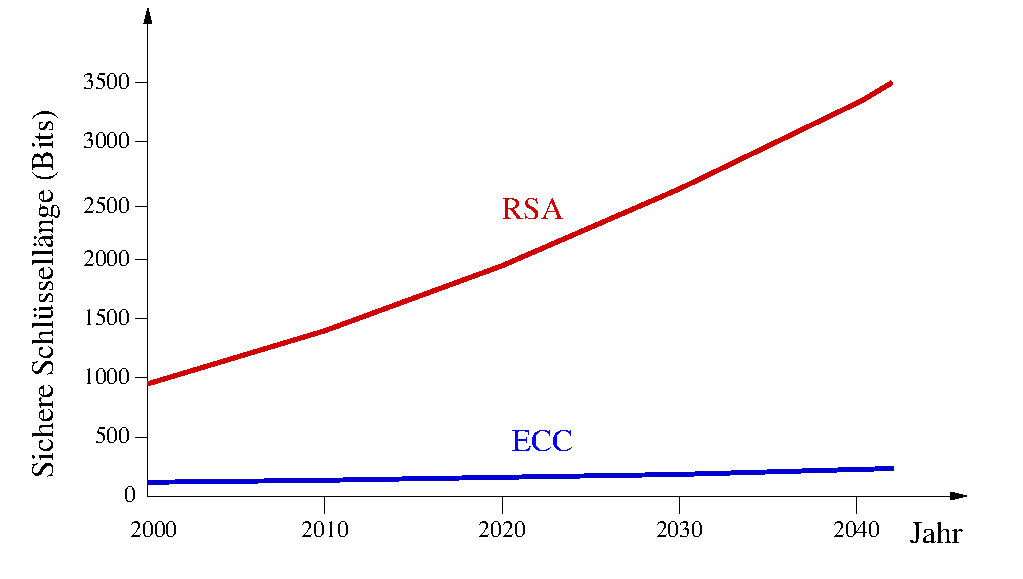
\includegraphics[scale=0.7]{figures/RSAKeyLength-2}
\caption{Prognosis of the key lengths regarded to be safe for RSA and
  for elliptic curves\vspace{1ex}} 
\label{RSAKeylength}
\end{center}
\end{figure}

In addition, a digital signature can be processed 10-times faster with ECC
than with RSA.  However, verification of a given signature is still more
efficient with RSA than with ECC. Refer to
figure~\ref{ThousandBitMultiplications} (source: Dr.~J.\ Merkle,
Elliptic-Curve Cryptography Workshop, 2001) for a comparison.  The reason is that
RSA public keys can be chosen relatively small as long as the secret key is
long enough.

% -> Figure 2
\begin{figure}[ht]
\begin{center}
\vspace{1.5cm}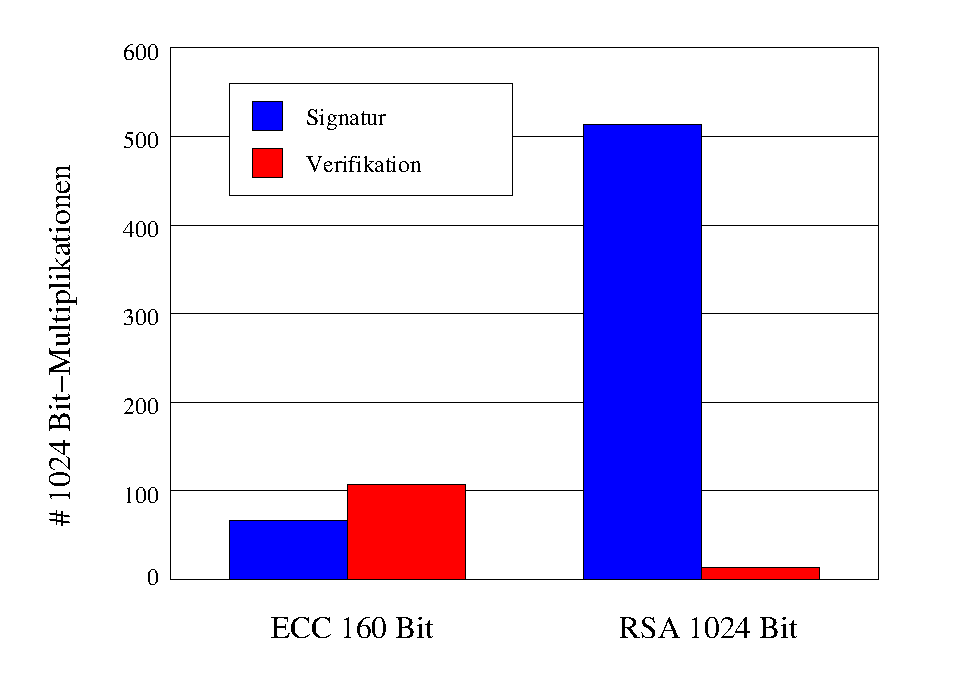
\includegraphics[scale=0.7]{figures/ECCRSA}
\caption{Comparison of signing and verification time for RSA and elliptic curves} 
\label{ThousandBitMultiplications}
\end{center}
\end{figure}

Nevertheless, thin clients like smart cards usually have to store the (long)
secret key and have to process a digital signature rather than verify one.
Therefore, there is a clear advantage in using ECC in terms of efficiency.
\par
\smallskip
Nowadays, the major problem with ECC implementations is the lack of
standardization. There is only one way to implement RSA, but there are many
ways for ECC: One can work with different sets of numbers, different (elliptic)
curves --- described by parameters\footnote{%
See chapter \ref{ECC-Crypto}
} --- , and a variety of representations of the elements on the curve. Each
choice has its advantages and disadvantages, and one can certainly construct
the most efficient for each application. However, this causes problems in
interoperability. But if all ECC-tools should be able to communicate with each
other, they will have to support all different algorithms, which might put the
advantage of efficient computation and the need of less storage capacity to the
contrary.

\begin{sloppypar}
Therefore, international standardization organizations like IEEE (P1363),
ASC (ANSI X9.62, X9.63), ISO/IEC as well as major players like RSA labs or
Certicom have recently started standardization initiatives. While the IEEE
only describes the different implementations, the ASC has explicitly stated
10 elliptic curves and recommends their usage. The advantage of the ASC
approach is that one needs only a single byte to indicate which curve is
meant. However, it is not yet clear whether the ASC curves will become a de
facto standard.
\end{sloppypar}

Although we see no need to replace RSA in any application today\footnote{%
Current information about the security of the RSA algorithm can be found in 
chapter \ref{SecurityRSA}.}, one should
take the usage of ECC-based tools into consideration whenever a new system
is set up --- in particular, when the tool should be available beyond 2005\footnote{%
Compare the recommendation of GISA: ``Fitting Crypto Algorithms'' from October 24th, 2002.
}. More current discussions about the security of ECC can be found in chapter xxxxxxxxxxxxxx


% -----------------------------------------------------------------------------
\section{Elliptic curves -- history}

Mathematicians have been researching elliptic curves for over 100 years.
Over the course of time, many lengthy and mathematically complex results
have been found and published which are connected to elliptic curves. 
A mathematician would say that elliptic curves (or the mathematics behind
them) are widely understood. This research was originally purely 
mathematical. That is to say, elliptic curves were investigated, for 
example, in the mathematical areas of number theory and algebraic 
geometry, which are generally highly abstract. Even in the recent
past, elliptic curves played an important role in pure mathematics.
In 1993 and 1994, Andrew Wiles\index{Wiles, Andrew} published 
mathematical works that triggered enthusiasm far beyond the specialist
audience. In these works, he proved a conjecture put forward in the 1960's.
To put it short, this conjecture was concerned with the connection 
between elliptic curves and what are called module forms. What is
particularly interesting for most people is that the works of Wiles
also proved the famous second theorem of Fermat. Mathematicians had
spent centuries (Fermat lived from 1601 to 1665) trying to find a
strict proof of this theorem. Understandably, therefore, Wiles' proof
got a good response. Fermat formulated his theorem as follows 
(written in the border of a book):

\begin{quote} {\em
Cubum autem in duos cubos, aut quadratoquadratum in duos quadratoquadratos, et
generaliter nullam in infinitum ultra quadratum potestatem in duos ejusdem
nominis fas est dividere: cujus rei demonstrationem mirabilem sane detexi. Hanc
marginis exiguitas non caperet.
} \end{quote}

With a free translation, using the denotation of modern mathematics, this means: \\
No positive whole numbers $x, y$ and $z$ greater than zero exist such that
$x^n +y^n = z^n$ for $n>2$. I have found an amazing proof of this fact, but there is
too little space within the confines of this book to include it.

This is truly amazing: A statement that is relatively simple to understand (we
are referring to Fermat's second theorem here) could only be proved after such a
long period of time, although Fermat himself claimed to have found a proof.
What's more, the proof found by Wiles is extremely extensive (all of Wiles
publications connected with the proof made up a book in themselves). This should
therefore make it obvious that elliptic curves are generally based on highly
complex mathematics.

Anyway that's enough about the role of elliptic curves in pure mathematics. 
In 1985 Neal Koblitz\index{Koblitz, Neal} and Victor Miller\index{Miller, Victor}
independently suggested using elliptic curves in cryptography. Elliptic 
curves have thus also found a concrete practical application. 
Another interesting area of application for elliptic curves is for
factorizing whole numbers \index{factorization} (the RSA cryptographic system
is based on the \index{complexity} difficulty/complexity of finding prime
factors of an extremely large number;  compare section \ref{SecurityRSA}.).
In this area, procedures based on elliptic curves have been investigated and
used since 1987 (compare section \ref{ECC-Factorization}). \\
There are also prime number tests\index{prime number!test} based on elliptic
curves.
% (s. Anmerkung U. Kuehn)

Elliptic curves are used differently in the various areas. Encryption
procedures based on elliptic curves are based on the difficulty of a problem
known as elliptic curve discrete logarithm\index{logarithm problem!discrete}.
The factorization of whole numbers uses the fact that a large number of
elliptic curves can be generated for a natural composite number $n$ with
several prime factors; however, these curves are not then groups for composite
$n$. More information about this can be found under the chapter \ref{ECC-Factorization}.



% -----------------------------------------------------------------------------
\section{Elliptic curves -- mathematical basics}

This section provides information about \index{group} {\em groups} and
\index{field} {\em fields}.

% -----------------------------------------------------------------------------
\subsection{Groups}

Because the term {\em group} is used differently in everyday language than in
mathematics, we will, for reasons of completeness, begin by introducing the
essential statement of the formal definition of a group:
\begin{itemize}
   \item A group is a non-empty set $G$ on which an operation ``$\cdot$''.
	 The set $G$ is closed under this operation, which means that for
	 any two elements $a, b$ taken from $G$, performing the operation
	 on them gives an element in $G$, i.e. $ab=a\cdot b$ lies in $G$.
   \item For all elements $a, b$ and $c$ in $G$: $(ab)c = a(bc)$ (associative law).
   \item There exists an element $e$ in $G$ that behaves neutrally with respect
	 to the operation $\cdot$. That means that for all a in the set $G: ~ae = ea = a$.
   \item For each element $a$ in $G$ there exists a so-called
	 inverse\footnote{The inverse is uniquely determined because if $x,y\in G$
	 are each inverse to $a$, i.e. $ax=xa=e$ and $ay=ya=e$, then
         $x=xe=x(ay)=(xa)y=ey=y$.}
	 element $a^{-1}$ in $G$ such that: $aa^{-1} = a^{-1}a = e$.
\end{itemize}
If also $ab = ba$ (commutative law) for all $a, b$ in $G$, then we call the group an {\em Abelian} group.

Since we may define different operations on the same set, we distinguish
them by giving them different names (e.g.\ $+$ addition or $\cdot$ multiplication).

The simplest example of an (Abelian) group is the group of whole numbers under
the standard operation of addition. The set of whole numbers is denoted as
${\mathbb Z}$. ${\mathbb Z}$ has an infinite number of elements, because
${\mathbb Z} = \{ \cdots, -4, -3, -2, -1, 0, 1, 2, 3, 4, \cdots\}$. For example, the
operation of $1+2$ lies in ${\mathbb Z}$, for $1+2 = 3$ and $3$ lies in
${\mathbb Z}$. The neutral element in the group ${\mathbb Z}$ is $0$. The
inverse element of $3$ is $-3$, for $3+(-3) = 0$.

For our purpose, so-called {\em finite} groups play an important role. This means that these exists a set
$\mathcal{M}$ with a fixed number of elements and an operation $+$ such that the
above conditions are fulfilled. One example of this is any set ${\mathbb Z}_n$
where ${\mathbb Z}_n = \{0, 1, 2, 3, \cdots, n-1\}, n$ is a positive whole number
and the operation is addition mod $n$, i.e. $a$ and $b$ in ${\mathbb Z}_n$ are
subject to the operation $a+b \;{\rm mod~} n$.

\paragraph*{Cyclic groups}\index{group!cyclic}
Cyclic groups\footnote{Cyclic groups can be in general also endless like
the additive group of the integer numbers. We consider here only finite
cyclic groups.} are those groups $G'$ that possess an element $g$
from which the group operation can be used to generate all other
elements in the group. This means that for each element $a$ in
$G'$ there exists a positive whole number $i$ such that if $g$ is
subject to the operation $i$ times (i.e. ``$g\cdot i$''),
$g+g+\cdots+g = a$ (additive group) or $g^i = g\cdot g \cdots g = a$
(multiplicative group). The element $g$ is the {\em generator} of
the cyclic group --- each element in $G'$ can be generated using
$g$ and the operation.

\paragraph*{Group order}
Now to the order of an element of the group: Let $a$ be in $G$. The smallest
positive whole number $r$ for which $a$ subject to the operation with itself $r$
times is the neutral element of the group $G'$ (i.e.: $r \cdot a = a+a+\cdots+a =
e$ respectively $a^r = e$), is called the {\em order} of $a$.

The order of the group is the number of elements in the set $G$.


% -----------------------------------------------------------------------------
\subsection{Fields}

In mathematics, one is often interested in sets on which at least two (group)
operations are defined --- frequently called addition and multiplication.
Most prominent are so called fields.

A field is understood to be a set $K$ with two operations
(denoted as $+$ and $\cdot$) which fulfils the following conditions:
\begin{itemize}
   \item The set $K$ forms an Abelian group together with the operation $+$
(addition), where $0$ is the neutral element of the operation $+$.
   \item The set $K\setminus\{ 0\}$ also forms an Abelian group
together with the operation $\cdot$ (multiplication).
   \item For all elements $a, b$ and $c$ in $K$, we have $c\cdot (a+b) = c \cdot a + c
\cdot b$ and $(a+b) \cdot c = a \cdot c + b \cdot c$ (distributive law).
\end{itemize}

Fields may contain an infinite number of elements (e.g.\ the field of real numbers).
They are called {\em infinite} fields. In contrast we call a field
{\em finite}, if it contains only a finite number of elements
(e.g.\ ${\mathbb Z}_p = \{0, 1, 2, 3, \cdots, p-1\}$, where $p$
is a prime. ${\mathbb Z}_p$ with addition mod $p$ and multiplication
mod $p$).
\index{field!characteristic}
\paragraph*{Characteristic of a field}
Let $K$ be a field and $1$ be the neutral element of $K$ with
respect to the multiplicative operation ``$\cdot$''. Then the characteristic
of $K$ is said to be the order of $1$ with respect to the additive operation.
This means that the characteristic of $K$ is the smallest positive integer $n$
such that $$ \underbrace{1+1+\dots+1}_{\hbox{$n$ times}} =0 .
$$
If there is no such $n$, i.e. if $1+1+\dots+1\ne 0$ no matter how many $1$s we add, then we call $K$ a field
with characteristic $0$.

Thus, fields with characteristic $0$ are infinite since they contain the
(pairwise distinct) elements $1$, $1+1$, $1+1+1$, \dots. On the other hand,
fields with finite characteristic may by finite or infinite.

If the characteristic is finite, it has to be prime. This fact can easily be proved: Assume $n=pq$, $p,q<n$, is the characteristic of a field $K$. By definition of $n$, the elements $\bar p=\underbrace{1+1+\dots+1}_{\hbox{$p$ times}}$, $\bar q=\underbrace{1+1+\dots+1}_{\hbox{$q$ times}}$ of $K$ are not equal to $0$. Thus, there exist inverse elements $\bar p^{-1},\bar q^{-1}$ with respect to multiplication. It follows that $(\bar p\bar q)(\bar p^{-1}\bar q^{-1})=1$, which contradicts the fact that $\bar p\bar q=\bar n=\underbrace{1+1+\dots+1}_{\hbox{$n$ times}}=0$ and, hence, $\underbrace{(\bar p\bar q)}_{=0}(\bar p^{-1}\bar q^{-1})=0$.

\begin{remark}{:}\\
The field of real numbers has the characteristic $0$; the field ${\mathbb Z}_p$ has
the characteristic $p$. If $p$ is not prime, ${\mathbb Z}_p$ is not a field at all.
\end{remark}

The most simple field is ${\mathbb Z}_2=\{ 0,1\}$. It contains only two elements, the neutral elements with respect to addition and multiplication. In particular, we have $0+0=0$, $0+1=1+0=1$, $1+1=0$, $1\cdot 1=1$, $0\cdot 0=0\cdot 1=1\cdot 0=0$.

\index{field!finite}
\paragraph*{Finite Fields}
As mentioned above, each finite field has a characteristic $p\ne 0$, where $p$ is a prime. On the other hand, given a prime $p$ there is a field which has exactly $p$ elements, that is ${\mathbb Z}_p$.

However, the number of elements of a field need not be prime in general. For example, it is not hard to construct a field with $4$ elements\footnote{%
The set $K=\{0,1,a,b\}$ fitted with the operation defined in the tabular below is a field:\\
$
\begin{array}{|c||c|c|c|c|} 
\hline 
+ & 0 & 1 & a & b \\
\hline \hline
0 & 0 & 1 & a & b \\
\hline 
1 & 1 & 0 & b & a \\
\hline 
a & a & b & 0 & 1 \\
\hline 
b & b & a & 1 & 0 \\
\hline 
\end{array} \qquad {\rm ~und~} \qquad
\begin{array}{|c||c|c|c|c|} 
\hline 
\cdot & 0 & 1 & a & b  \\
\hline \hline
0 & 0 & 0 & 0 & 0 \\ 
\hline 
1 & 0 & 1 & a & b \\ 
\hline 
a & 0 & a & b & 1 \\ 
\hline 
b & 0 & b & 1 & a \\
\hline 
\end{array} 
$  \\
}.

One can show that the order of any field is a prime power (i.e. the power of a prime number). On the other hand, we can construct a field with $p^n$ elements for any given prime $p$ and positive integer $n$. Since two fields that have the same number of elements can not be distinguished\footnote{If $K,K'$ are fields with $k=p^n$ elements, then there is a one-to-one map $\varphi:K\to K'$, that respects the arithmetic of the field. Such a map is called an isomorphy. Isomorphic fields mathematically behave in the same way so that   it makes no sense to distinguish between them. For example, ${\mathbb Z}_2$ und $K'=\{ ZERO,ONE\}$ with zero-element $ZERO$ and one-element $ONE$ are isomorphic. We note that mathematical objects are only defined by their mathematical properties.}, we say that there is {\bf the field with $p^n$ elements} and denote it by $GF(p^n)$. Here $GF$ stands for {\it Galois Field} to commemorate the French Mathematician Galois.

The fields $GF(p)$ of prime order play a prominent role. They are called prime fields and often denoted by ${\mathbb Z}_p$\footnote{For prime fields additive as well as multiplicative group are cyclic. Furthermore, each field $GF(p^n)$ contains a subfield that is isomorphic to the prime field ${\mathbb Z}_p$.}.


% -----------------------------------------------------------------------------
\section{Elliptic curves in cryptography}\label{ECC-Crypto}

In cryptography elliptic curves are a useful tool.\footnote{%
We write ``elliptic-curve cryptography'' with a hyphen, according to ``public-key cryptography''. Sadly, this isn't used consistently in the literature.
}

Such curves are described by some equation. A detailed analysis has shown that curves of the form\footnote{This curve is given by the zeros of a {\it polynomial}\index{polynomial} $F$ of degree three in three variables. In general, expressions of the form
$P=\sum_{i_1,\dots,i_n\in\N_0} a_{i_1\dots i_n} x_1^{i_1}\dots x_n^{i_n}$ with coefficients $a_{i_1\dots i_n}\in K$ are called polynomials in $n$ variables $x_1,\dots,x_n$ with underlying field $K$, if ${\rm deg\,} P:=\max\{i_1+\dots +i_n: a_{i_1\dots i_n}\ne 0\}$ is finite, i.e. the sum has only finitely many non-zero terms (monomials). The sum of the exponents of the variables of each term of the sum is at most $3$, at least one term of the sum has a single variable with $3$ as value of the according exponent.}
\begin{equation}
 F(x_1,x_2,x_3)=-x_1^3+x_2^2x_3+a_1x_1x_2x_3-a_2x_1^2x_3+a_3x_2x_3^2-a_4x_1x_3^2-a_6x_3^3=0,
\label{eccbasisgleichung}
\end{equation}
are especially useful. The variables $x_1,x_2,x_3$ and parameters $a_1,\dots,a_4,a_6$ are elements of a given field $K$, which has certain properties that are make it useful from the cryptographic point of view. The underlying field $K$ might be the well known field of real numbers or some finite field (see last section).
In order to obtain a cure that is useful for cryptography, the parameters have to be chosen in a way that the following conditions hold
$$ \frac{\partial F}{\partial x_1}\ne 0, \quad \frac{\partial F}{\partial x_2}\ne 0, \quad
\frac{\partial F}{\partial x_3}\ne 0 .
$$
We identify points on the curve that can be derived from each over by multiplying each component with some scalar. This makes sense since $(x_1,x_2,x_3)$ solves (\ref{eccbasisgleichung}) if and only if $\alpha (x_1,x_2,x_3)$ ($\alpha\ne 0$) does. Formally, this means that we consider classes of equivalent points instead of single points, where points are called equivalent if one is the scalar multiple of the other one.
\\ If we put $x_3=0$ in the basic equation (\ref{eccbasisgleichung}), then this equation collapses to $-x_1^3=0$, leading to $x_1=0$. Thus, the equivalence class which includes the element $(0,1,0)$ is the only one that contains a point with $x_3=0$. For all points on the curve that are not equivalent to $(0,1,0)$, we may apply the following transformation
$$ K\times K\times (K\setminus\{0\})\ni (x_1,x_2,x_3) \mapsto (x,y):=\left( \frac{x_1}{x_3}, \frac{x_2}{x_3}\right) \in K\times K \, ,
$$
which reduces the number of variables to two instead of three. We note that the
basic equation (\ref{eccbasisgleichung}) $F(x_1,x_2,x_3)=0$  was chosen in a
way that this transformation leads to the famous so-called
Weierstrass-Equation\footnote{Karl Weierstrass\index{Weierstrass, Karl}, 31.10.1815$-$19.12.1897, German
mathematician, famous for his rigorous formal approach to mathematics.} holds
\begin{equation}
 y^2+a_1xy+a_3y = x^3+a_2x^2+a_4x+a_6 \, .
\label{ell}
\end{equation}
Since all but one point (i.e. equivalence class) of the elliptic curve can be described using equation (\ref{ell}), this equation is often called the elliptic equation, and its solutions written as
$$ {\bf E} = \left\{(x,y)\in K\times K \, |\, y^2+a_1xy+a_3y = x^3+a_2x^2+a_4x+a_6  \right\} \cup \{{\cal O} \}.
$$
Here, ${\cal O}$ represents the point $(0,1,0)$ that is loosely speaking mapped to infinity by the transformation (division by $x_3$) that reduces the three variables to two.

% -> Figure 3
\begin{figure}[ht]
\begin{center}
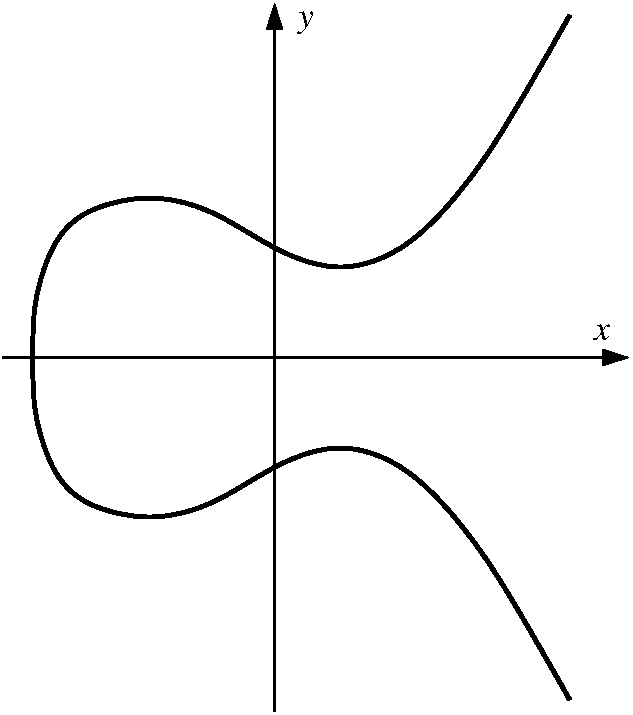
\includegraphics[scale=0.60]{figures/elliptic-curve}
\caption{Example of an elliptic curve with the real numbers as underlying field\vspace{1ex}} 
\label{ExampleEllipticCurve}
\end{center}
\vskip -10 pt
\end{figure}

In contrast to figure \ref{ExampleEllipticCurve} only finite fields $K=GF(p^n)$ are used in elliptic-curve cryptography. The reason is loosely speaking that in modern communication engineering data processing is always based on discrete data (simply because computers accept only discrete data).

For practical reasons, it turned out to be useful to take either $GF(p)$ with a large prime $p$ or $GF(2^n)$ with a (large) positive integer $n$. Using $GF(p)$ has the advantage of providing a relatively simple arithmetic; on the other hand $GF(2^n)$ allows a binary representation of each element that supports the way computers work. Other fields like, for example, $GF(7^n)$ do not have any of these advantages and are, thus, not considered, although there is no mathematical reason why they should not.

A coordinate transformation can result in a simpler version\footnote{Such a coordinate transformation is combination of a rotation and a dilatation of the coordinate system without changing the elliptic curve itself.} of the Weierstrass equation\index{Weierstrass, Karl}. Depending whether $p>3$, different transformations are used, and we obtain
\begin{itemize}
\item in case of $GF(p)$, $p>3$, the elliptic curve equation of the form
\begin{equation}
 y^2 = x^3 + ax + b
\label{ellp}
\end{equation}
with $4a^3+27b^2\ne 0$
\item in case of $GF(2^n)$ the elliptic curve equation of the form 
\begin{equation}
 y^2+xy = x^3 + ax^2 + b
\label{ell2}
\end{equation}
with $b\ne 0$\footnote{The form (\ref{ellp}) is called the standard form of the Weierstrass-equation\index{Weierstrass, Karl}. If the characteristic of the field is $2$ or $3$, we obtain $4=0$ respectively $27=0$, which means that the condition on parameters $a,b$ collapse. Loosely speaking, this is the reason why the transformation to the standard form does not work in these cases.}.
\end{itemize}
This conditions on the parameters $a,b$ ensure that the elliptic equation can be used in the context of cryptography\footnote{Formally we call such curves non singular.}.

Let $|E|$ denote the number of elements of an elliptic curve $E$ given an underlying field $GF(k)$ (for practical reasons either $k=p$ with $p$ prim or $k=2^n$). Then Hasse's theorem\cite{ec:Silverman1992} yields $| \, |E| - k-1\,| \le 2\cdot \sqrt{k}$. This inequality is equivalent to $k+1 - 2\sqrt{k} < |E| < k+1+2\sqrt{k}$. In particular, this means that the number of elements of an elliptic curve is approximately $k$ (for large $k$). 


% -----------------------------------------------------------------------------
\section{Operating on the elliptic curve}

In order to work with elliptic curves in practice, we define an operation (often written in an additive way $+$) on the set of points on the curve. If we have a curve over the field $GF(p)$, we define the commutative operation $+$ by
\begin{enumerate}
\item $P+{\cal O}={\cal O}+P=P$ for all $P\in E$,
\item for $P=(x,y)$ and $Q=(x,-y)$ we set $P+Q={\cal O}$,
\item for $P_1=(x_1,x_2),P_2=(x_2,y_2)\in E$ with $P_1,P_2\ne {\cal O}$ and $(x_2,y_2)\ne (x_1,-y_1)$ we set $P_3:=P_1+P_2$, $P_3=(x_3,y_3)$ defined by
$$ x_3:=-x_1-x_2+\lambda^2 \, , \qquad y_3:=-y_1+\lambda (x_1-x_3)
$$
with the auxiliary quotient
$$ \lambda:=\left\{ \begin{array}{cl} \frac{y_1-y_2}{x_1-x_2} & {\rm if~} P_1\ne P_2, \\
                                     \frac{3x_1^2+a}{2y_1} & {\rm if~} P_1=P_2. \end{array} \right.
$$
\end{enumerate}
In particular, we obtain $-P=(x,-y)$ for $P=(x,y)\in E$.

If we deal with a curve over the field $GF(2^n)$, we define the operation $+$ in an analogous way by
\begin{enumerate}
\item $P+{\cal O}={\cal O}+P=P$ for all $P\in E$,
\item for $P=(x,y)$ and $Q=(x,x+y)$ we set $P+Q={\cal O}$,
\item for $P_1=(x_1,x_2),P_2=(x_2,y_2)\in E$ with $P_1,P_2\ne {\cal O}$ and $(x_2,y_2)\ne (x_1,x_1+y_1)$ we set $P_3:=P_1+P_2$, $P_3=(x_3,y_3)$ defined by
$$ x_3:=-x_1+x_2+\lambda+\lambda^2+a \, , \qquad y_3:=y_1+x_3+\lambda (x_1+x_3)
$$
with auxiliary quotient
$$ \lambda:=\left\{ \begin{array}{cl} \frac{y_1+y_2}{x_1+x_2} & {\rm if~} P_1\ne P_2, \\
                                   x_1+\frac{y_1}{x_1} & {\rm if~} P_1=P_2. \end{array}\right.
$$
\end{enumerate}
In particular, we obtain $-P=(x,-y)$ for $P=(x,y)\in E$.

(Note that $-(-P)=(x,x+(x+y))=(x,2x+y)=(x,y)$, since the underlying field
has characteristic $2$.)\footnote{%
An animation of the addition of points
on elliptic curves can be found on the Certicom\index{Certicom} homepage \\
\url{http://www.certicom.com/index.php/ecc-tutorial}\\
See also the web link about the \hyperlink{ec:Web-Link:Java_Laubrock}
{Java-Tutorial} at the end of this chapter.
}

One can verify that $+$ defines a group operation on the set $E\cap\{\cal O\}$.
In particular this means that the sum of two points is again a point on the
elliptic curve. How his operation works is geometrically visualized in the
following section.

% \newpage
\begin{figure}[htbp]
\subsection*{How to add points on an elliptic curve}
The following figures show how points on an elliptic curve over the field of real numbers are summed up using affine coordinates.
We note that the point infinity ${\cal O}$ cannot be shown in the affine plane.  
\begin{center}
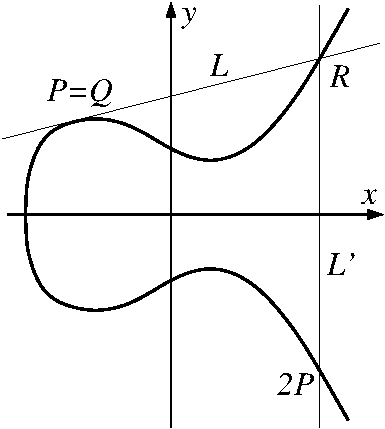
\includegraphics[scale=1.08]{figures/ec-mult2}
\caption{Doubling of a point} 
\vspace{\floatsep}
\vskip +20 pt
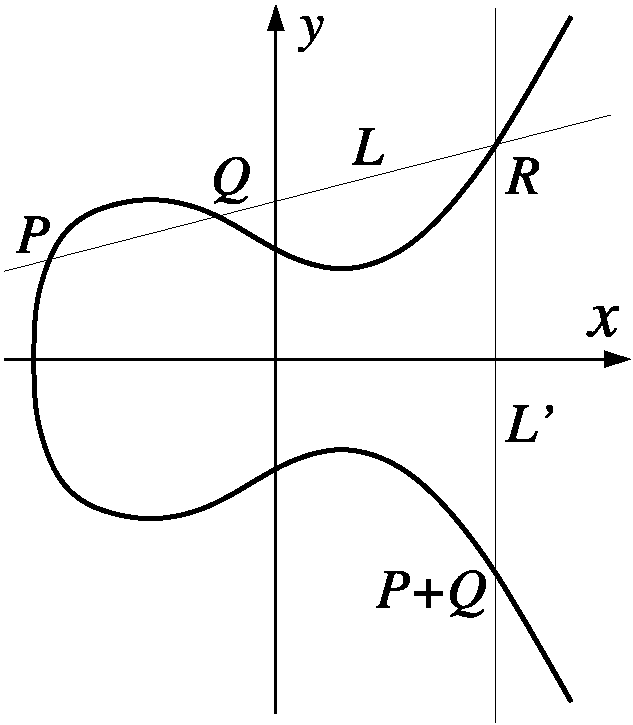
\includegraphics[scale=0.65]{figures/ec-add}
\caption{Summing up two different points over the real number field} % \footnotemark }
\end{center}
\end{figure}
\enlargethispage{+20pt}
\newpage


% -----------------------------------------------------------------------------
\section{Security of elliptic-curve cryptography: The ECDLP}

As mentioned above in section \ref{ECC-Crypto}, we only consider elliptic curves over the finite\footnote{Discrete in contrast to continuous.} fields $GF(2^n)$ or $GF(p)$ (for a large prime $p$). This means that all parameters that describe the curve are taken from this underlying field. If $E$ is an elliptic curve over such a field and $P$ is a point on the curve $E$, then we can derive for all positive integers $m$
$$ mP := \underbrace{P+P+\dots+P}_{\hbox{$m$ times}} \, .
$$
Looking on this operation from the cryptographic point of view, it turns out to be very interesting by the following reason: On the one hand one needs only $\log m$ operations to calculate $mP$ --- one simply has to calculate $P$, $2P$, $2^2P$, $2^3P$, \dots, write $m$ in a binary form and finally add all these multiples $2^kP$ of $P$ with respect to the binary representation of $m$ --- on the other hand it seems to be very hard to find $m$ given $P$ and $Q=mP$ on $E$. Of course, we may simply calculate $P,2P,3P,4P,5P,\dots$ and compare each of them with $Q$. But this will take as much as $m$ operations.

Yet there is no algorithm known that efficiently derives $m$ given $P$ and $G$. The best algorithms known so far need about $\sqrt{q}$ operations where $q$ is the (largest) prime factor of $p-1$, in case the underlying field is $GF(p)$; here $m$ should be between $1$ and $q$ liegen so that one needs at most $\log q$ operations to calculate $mP$. However, the quotient $\frac{\sqrt{q}}{\log q}$ tends to $+\infty$ very fast for large $q$.

If we choose the parameters sufficiently large (for example, let $p$ be prime and at least $160$ bits long), an computer will easily be able to calculate $mP$ (in less than a second). The {\it inverse problem} however, to derive $m$ from $mP$ and $P$, can (still) not be solved in reasonable time.

This problem is known as the ``Elliptic Curve Discrete Logarithm Problem'' (for short ECDLP\index{ECDLP}).

\vskip +5 pt

In elliptic-curve cryptography we formally look at points on the elliptic curve as elements of a group with point addition $+$ as operation. Furthermore, we use only elliptic curves that have a sufficiently large number of points. However, in special cases curves may be weak and not useful due to other reasons. For such special cases the ECDLP can be much easier to solve than in the general case. This means that one has to look carefully at the parameters when choosing an elliptic curve for cryptographic applications.

Not useful for cryptography are {\em a-normal} (that are curves over ${\mathbb Z}_p$,
for which the set ${\bf E}$ consists of exactly $p$ elements) and {\em supersingular} curves (that are curves, for which the ECDLP can be reduced to the ``normal'' discrete logarithms in another, smaller finite field). This means that there are cryptographically useful and non-useful elliptic curves. Given the parameters $a$ and $b$, it is possible to determine whether a curve is useful or not. In many publications one can find parameters that turned out to be useful for cryptography. The open (scientific) discussion guarantees that these results take into account latest research.
\vskip +5 pt

Given a secure curve, the time that is needed to solve the ECDLP is strongly correlated with parameter $p$ in case $GF(p)$ respectively $n$ in case of $GF(2^n)$. The larger these parameters become, the more time an attacker needs to solve the ECDLP --- at least with the best algorithms known so far. Experts recommend bit-lengths of $200$ for $p$ for secure curves. A comparison with RSA modulus length shows why elliptic curves are so interesting for applications. We note that the computation effort for signing and encryption is closely related to the bit-length of the parameters. In addition the initiation process, i.e. the generation of the private-public-key-pair, becomes more complicated the larger $p$ is. Thus, one looks for the smallest parameters that still come along with the security required. It is remarkable that a length of $200$ bits for $p$ is sufficient to construct a {\em good} elliptic curve that is as secure as RSA with a $1024$ bit \index{RSA!modulus} RSA modulus (as far as we know today). For short, the reason for this advantage of ECC lies in the fact that the best algorithms known for solving the ECDLP need exponential time while the best algorithms for factorizing are sub-exponential (number field sieve, quadratic sieve or factorizing with elliptic curves). Hence, the parameters for a cryptosystem that is based on the problem of {\em factorizing large integers} have to be larger than the parameters for a system based on ECDLP.


% -----------------------------------------------------------------------------
\section{Encryption and signing with elliptic curves}

\begin{sloppypar}
  The {\em elliptic curve discrete logarithm
    problem}\index{problem of discrete logarithm} (ECDLP) \index{ECDLP} is the basis for elliptic-curve cryptography. Based on this problem, there are different signature schemes. In order to apply one of these, we need:
\end{sloppypar}
\begin{itemize}
    \item An elliptic curve {\bf E} with an underlying field $GF(p^n)$.
    \item A prime $q\ne p$ and a point $G$ on the elliptic curve ${\bf E}$ with order $q$. This means that $qG={\cal O}$ and $rG\ne {\cal O}$ for all $r\in \{1,2,\dots,q-1\}$. Thus $q$ is a factor of the group order (i.e. the number of elements) $\#{\bf E}$ of $E$. Since $q$ is prime, $G$ generates a cyclic sub-group of ${\bf E}$ of order $q$.
\end{itemize}
The parameters mentioned are often called \index{domain parameter}
{\em Domain} parameter. They describe the elliptic curve ${\bf E}$ and 
the cyclic sub-group of ${\bf E}$ on which the signature scheme is based.

\par
%\smallskip
%{\bf Encryption:}
\subsection{Encryption}

Using elliptic curves one can construct a key exchange protocol based on the Diffie-Hellman protocol \index{Diffie-Hellman} (see chapter \ref{DH-KeyExch}). The key exchanged can be used for a subsequent symmetric encryption. We note that in contrast to RSA there is no pair of private and public key that can be used for encryption and decryption!

In the notation of elliptic curves, the Diffie-Hellman protocol reads as follows: First both partners (A und B) agree on a group $G$ and an integer $q$. Then they choose $r_A,r_B\in\{1,2,\dots,q-1\}$ at random, derive the points $R_A=r_AG$, $R_B=r_BG$ on the elliptic curve and exchange them (using an insecure channel). After that A easily obtains $R=r_AR_B$; B gets the same point ($R=r_Ar_B G$) by calculating $r_BR_A=r_Br_AG=r_Ar_BG=R$. We note that $R_A,R_B$ are easy to derive as long as $r_A$ respectively $r_B$ are known $G$. However, the inverse operation, to get $R_A$ respectively $R_B$ from $r_A$ respectively $r_B$ is hard.
\\ Using the best algorithms known so far, it is impossible for any attacker to obtain $R$ without knowing either $r_A$ or $r_B$ --- otherwise he would have to solve the ECDLP.

In order to prohibit a ``Man-in-the-middle"{}~attack, one may sign the values $G,q,R_A,R_B$ as described in chapter \ref{Impersonalisierungsattacke}.


\par
%\smallskip 
%{\bf Signing:}
\subsection{Signing}

Using the \index{DSA} DSA signature scheme, one can proceed as follows: The signing party chooses a (non-trivial) number $s\in{\mathbb Z}_q$, which will be the private key, and publishes $q$, $G$ and $R=sG$. We note that $s$ cannot be obtained from $G$ and $R$ are not sufficient --- a fact on which the security of the signature scheme is based.

Given the message $m$, which should be signed, one first constructs a digital finger print using a hash-algorithm $h$ such that $h(m)$ has its values in $\{0,1,2,\dots, q-1\}$. Thus, $h(m)$ can be considered as an Element of ${\mathbb Z}_q$. Then the signing party chooses a random number $r\in{\mathbb Z}_q$ and derives $R=(r_1,r_2)=rG$. We note that the first component $r_1$ of $R$ is an element of $GF(p^n)$. This component will then be projected onto ${\mathbb Z}_q$, i.e. in case of $n=1$ it is interpreted as the remainder of an element of $\{0,1,\dots,p-1\}$ divided by $q$. This projection of $r_1$ onto ${\mathbb Z}_q$ is denoted by $\bar r_1$. Then one determines $x\in {\mathbb Z}_q$ such that
$$ rx-s\bar r_1-h(m)=0 .
$$
The triple $(m,r_1,x)$ is then published as the digital signature of message $m$.

\par
%\smallskip 
%{\bf Signature Verification:}
\subsection{Signature verification}

In order to verify a signature, one has to build $u_1=h(m)/x$, $u_2=\bar r_1/x$ (in ${\mathbb Z}_q$ and derive
$$ V=u_1G+u_2Q .
$$
Since we have $Q=sG$, the point $V=(v_1,v_2)$ satisfies $v_1=u_1+u_2s$. We note that this operations take place in the field $GF(p^n)$. The projection of $GF(p^n)$ on ${\mathbb Z}_q$ mentioned above should be chosen in such a way that $\bar v_1=u_1+u_2s$ is an element of ${\mathbb Z}_q$. Then it follows that
$$ \bar v_1=u_1+u_2s=h(m)/x+\bar r_1 s/x=(h(m)+\bar r_1s)/x=rx/x=r .
$$
Since $R=rG$, we obtain $\bar v_1=\bar r_1$, i.e. $R$ and $V$ coincide modulo the projection onto ${\mathbb Z}_q$.


% -----------------------------------------------------------------------------
\hypertarget{faktell}{}
\section{Factorization using elliptic curves} \label{ECC-Factorization}

There are factorization%
\footnote{Especially John M. Pollard \index{Pollard, John M.} was involved
in the development of many different factorization algorithms; also at
factorization with ECC he was one of the leading heads. As an employee
of British Telekom he never published much. At the RSA data Security Conference
in 1999 he was awarded for his ``outstanding contributions in mathematics'':
\url{http://www.eff.org/Privacy/Crypto_misc/DESCracker/HTML/19990118_rsa_awards.html}.\\
In 1987 H.W. Lenstra published an often used factorization algorithm,
based on elliptic curves (see \cite{ec:Lenstra1987}).
}
algorithms based on elliptic curves%
\footnote{The biggest compound numbers currently 
factorized\index{factorization!factoring records} with elliptic curves have
about 80 decimal digits:\\
\url{http://www.loria.fr/~zimmerma/records/top50.html}.\\
See also the web link about the \hyperlink{Lenstra2}{ECMNET project}\index{ECMNET} at the end of this chapter.
}. 
More precisely, these procedures exploit the fact that elliptic curves can
be defined over ${\mathbb Z}_n$ ($n$ composite number). Elliptic curves 
over ${\mathbb Z}_n$ do not form a group, because not every point on such 
an elliptic curve has an inverse point. This is connected with the fact 
that - if $n$ is a composite
number - there exist elements in ${\mathbb Z}_n$ that do not have an inverse
with respect to multiplication mod $n$. In order to add two points on an
elliptic curve over ${\mathbb Z}_n$, we can calculate in the same way as on
elliptic curves over ${\mathbb Z}_p$. Addition of two points (on an elliptic
curve over ${\mathbb Z}_n$), however, fails if and only if a factor of $n$ has
been found. The reason for this is that the procedure for adding points on
elliptic curves gives elements in ${\mathbb Z}_n$ and calculates the inverse
elements for these (with respect to multiplication mod $n$) in ${\mathbb Z}_n$.
The extended \index{Euclidean algorithm} Euclidean algorithm is used here. If
the addition of two points (that lie of an elliptic curve over ${\mathbb Z}_n$)
gives an element in ${\mathbb Z}_n$ that does not have an inverse element in
${\mathbb Z}_n$, then the extended Euclidean algorithm delivers a genuine factor
of $n$.

Factorization using elliptic curves thus principally works as follows: 
Random curves over ${\mathbb Z}_n$ are selected, as well as random points
(that lie on this curve) and add them; you thus obtain points that also
lie on the curve or find a factor of $n$. 
Factorization algorithms based on elliptic curves
therefore work probabilistically. The opportunity of defining large number of
elliptic curves over ${\mathbb Z}_n$ allows you to increase the probability of
finding two points which you can add to obtain a factor of $n$. These procedures
are therefore highly suitable for parallelization.


% -----------------------------------------------------------------------------
\newpage
% \section{Implementing elliptic curves for educational purposes, pat\-ent aspects}
\section{Implementing elliptic curves for educational purposes}
\label{ec:Implementing-for-Education}

There are not many free programms offering ECC under a graphical user interface.
The following subsections explain which according functionality is available in
CrypTool and in SageMath.


% -----------------------------------------------------------------------------
\subsection{CrypTool}\index{CrypTool}

CT1 offers elliptic curves for the digital signature function%
\footnote{%
The dialog box, which appears in CT1\index{CrypTool 1} after clicking the menu
{\bf Digital Signatures/PKI \textbackslash{} Sign Message},
offers the EC methods ECSP-DSA and ECSP-NR.

} and for ECC-AES hybrid encryption%
\footnote{%
Within CT1\index{CrypTool 1} you can find this technique using the menu
path {\bf Crypt \textbackslash{} Hybrid}.

}.

It implements the basic algorithms for group operations, for generating elliptic
curves, for importing and exporting parameters for elliptic curves over finite
fields with $p$ elements ($p$ prime). The algorithms have been implemented in
ANSI C and comply with draft no. 8 of the IEEE P1363 work group {\em Standard
Specifications for Public Key Cryptography}

{\url{http://grouper.ieee.org/groups/1363}}.

The procedure implements the cryptographic primitives for generating and
verifying signatures for the variations of Nyberg-Rueppel signatures and
\index{DSA} DSA signatures based on elliptic curves.

Step-by-step point addition on elliptic curves is visualized in CT1\index{CrypTool 1} and JCT\index{JCrypTool}.%
\footnote{%
CT1: menu {\bf Digital Signatures/PKI \textbackslash{} Signature Demonstration
(Signature Generation)},\\
JCT (default perspective): menu {\bf Visuals \textbackslash{} Elliptic Curve
Calculations}.

}


% -----------------------------------------------------------------------------
\subsection{SageMath}
\label{ec:Sage_Massierer}
\index{SageMath}
\index{SageMath!code examples}

In SageMath elliptic curves are described at

\url{http://www.sagemath.org/doc/constructions/elliptic_curves.html}%
\footnote{%
According SageMath samples can be found at the "Published Worksheets" at
\url{http://www.sagenb.org/pub/}\\
- about Elliptic Curve: \url{http://www.sagenb.org/home/pub/606/} \\
- about Elliptic Curve El Gamal: \url{http://www.sagenb.org/home/pub/104/}, or at

  \noindent\hangindent=6pt\makebox[6pt][l]{-}%
  the "Elliptic Curve Cryptography (ECC) Tutorial"\\
  \url{http://www.williamstein.org/simuw06/notes/notes/node12.html}
  
}.

\noindent Additionally there is an exhaustive, interactive
\hyperlink{ec:Web-Link:Sage_Massierer}{ECC tutorial} by Maike Massierer.
This interactive introduction to Elliptic-Curve Cryptography is built up as
a SageMath notebook.

SageMath notebooks are running after a logon within a browser%
\footnote{%
If you installed SageMath on your own (Unix) server, you first have to enter at the
command line the command \verb#notebook()#.

}${}^,$\footnote{%
The ECC notebook of Maike Massierer needs the KASH3 library: Therefore e.g.\ with SageMath 4.2.1
the package ``kash3-2008-07-31.spkg'' has to be installed (command \verb#sage -i#).
}.

The ECC notebook\index{elliptic curve!ECC notebook}\index{Massierer, Maike} of
Massierer\footnote{%
Instructions to use an interactive SageMath notebook\index{SageMath!instructions interactive notebook}:
TODOTODO: Update for the new SageMathCloudxxxxxxxxxxxxx\\

  \noindent\hangindent=6pt\makebox[6pt][l]{-}%
  Public SageMath servers like \url{http://sage.mathematik.uni-siegen.de:8000} or
  \url{http://www.sagenb.org/} often offer running samples as "Published Worksheets",
  which you can run and download without login on. These worksheets are listed
  if you click on ``Published'' in the above right corner.

  \noindent\hangindent=6pt\makebox[6pt][l]{-}%
  Worksheets using the  \verb#interact# command currently need some additional
  todos for a user to work correctly: sign-in, make a copy and execute all
  commands again.\\
  This works as follows (described for the sagenb server and for the ECC tutorial):\\
 
  \noindent\hangindent=6pt\makebox[6pt][l]{-}%
  Sign-up for a SageMath notebook account at \url{http://sagenb.org/register}
  and sign in at \url{http://sagenb.org/}.

  \noindent\hangindent=6pt\makebox[6pt][l]{-}%
  Open the worksheet \url{http://sagenb.org/home/pub/1126/}.
  This contains the table of contents of the interactive ECC notebook.
  From here you can navigate via a click to the different chapters of the document.

  \noindent\hangindent=6pt\makebox[6pt][l]{-}%
  In the very top left corner, click \verb#Edit a copy# in order to create
  your own copy of the worksheet.

  \noindent\hangindent=6pt\makebox[6pt][l]{-}%
  Sometimes it's necessary at the beginning to re-evaluate the worksheet.
  Click in the left upper corner on \verb#Action -> Evaluate all#.

  \noindent\hangindent=6pt\makebox[6pt][l]{-}%
  Some of the applications still do not always work after opening a worksheet.
  Instead of nice output, they show lots of (blue) error messages.
  This normally can be solved quickly by clicking the gray  ``\%hide'' string:
  Then you get the code behind the graphics. Simply generate the graphics
  again with Shift-Enter.\\
  Even after doing this, the graphics code does not always disappear. Instead,
  it sometimes turns gray. Should this happen, click on the gray text,
  then click somewhere outside of the text box. The code will then
  disappear and leave you with a nice layout of the worksheet.

  \noindent\hangindent=6pt\makebox[6pt][l]{-}%
  Some of the ECC tutorial's content uses a special math fonts that are
  not installed by default with most browsers. When you notice that
  formulas are not displayed correctly or even get an error message
  about missing fonts from your browser, you need to install the jsMath
  fonts for a better layout.\\
  See \url{http://www.math.union.edu/~dpvc/jsMath/}
  and \url{http://pubpages.unh.edu/~jsh3/jsMath/}.\\
  After installing these fonts you can see the jsMath symbol at the lower border
  of your browser. If you click this symbol you can find the download page for
  the TIFF fonts. This fonts installation has to be done at every PC.

  \noindent\hangindent=6pt\makebox[6pt][l]{-}%
  According to the SageMath-support newsgroup there is work underway
  to create a system for using \verb#@interact# completely outside of the
  SageMath notebook (JS code within a static html pages).

}${}^,$\footnote{%
  Since 2008 this ECC notebook can be found at
    \url{http://sage.mathematik.uni-siegen.de:8000/home/pub/45/} (\verb!#45 to #52!).
  To logon in Siegen you have to allow port 8000 and Cookies.\\
  Since 2009 an updated version of this ECC notebook can be found at
    \url{http://sagenb.org/home/pub/1126/} (\verb!#1126 to #1133!).
}
consists of 8 parts (title page plus 7 chapters)
% "Titelseite" mit Inhaltsverzeichnis plus 7 Kapitel
and aims to let even beginners understand what elliptic curves are:

\begin{enumerate}
   \setcounter{enumi}{-1}
   \item ECC Notebook (title page and contents)
   \item Introduction and Overview
   \item Motivation for the use of Elliptic Curves in Cryptography
   \item Elliptic Curves in Cryptography
   \item Cryptographic Protocols in ECC
   \item Domain Parameter Generation for ECC Systems
   \item Conclusion and Further Topics
   \item References
\end{enumerate}


% -----------------------------------------------------------------------------
\newpage
\section{Patent aspects}\index{patent}

If the field $GF(2^n)$ is used instead of the prime field $GF(p)$, one has to make substantial changes in the implementation. The advantage of $GF(2^n)$ lies in the fact that calculations in $GF(2^n)$ can be implemented very efficiently using the binary representation. In particular, divisions are much easier to process compared to $GF(p)$ (this is particularly important in the signature scheme mentioned above where a division is needed for processing a signature as well as for the verification).

In order to achieve maximal gain in efficiency, one may choose a field that allows special basis like polynomial basis (useful for software implementations) or normal basis (best for hardware implementations). For special $n$ (like, for example, $n=163,179,181$) one may even combine both advantages. However, they are still non-standard.

Sometimes only the first component and one additional bit is used as representation of a point on the elliptic curve instead of the full two components. Since the first component together with the additional bit is sufficient to derive the full point, this representation minimizes the memory capacity needed. In particular, for normal basis this point compression can be implemented efficiently. In addition, the cryptographic protocols themselves become more effective. A disadvantage is, however, that {\it point compression} can be used for about half of all elliptic curves only and is protected under
US patent (US Patent 6141420, Certicon), causing additional costs.
In the general case $GF(p^n)$ (and also in case $n=1$) often so called affine or projective co-ordinates are used. Depending on the application, these co-ordinates may result in a gain in efficiency as well.

A comprehensive description of all implementations and their advantages and disadvantages would go far beyond the scope of this paper. We only want to state that there is a variety of possible implementations for elliptic-curve cryptography, much more than for RSA. Therefore, there are serious efforts to reduce this large to a small number of standard implementations. Some standardization committees even try to reduce the complexity by focusing on a small number of (prescribed) curves (ASC approach).

It is still not clear whether these standardization initiatives will be
successful or not. However, without agreed standards, ECC is not likely to
become a real alternative for RSA. The committees might be forced to act fast
if there was a break-through in factorization.

Current informationen about the patents situation can be found here\footnote{%
\url{https://en.wikipedia.org/wiki/Elliptic_curve_cryptography}\\
\url{https://en.wikipedia.org/wiki/ECC_patents}\\
\url{https://cr.yp.to/ecdh/patents.html} Bernstein, Daniel J. (2006-05-23): ``Irrelevant patents on elliptic-curve cryptography''. Retrieved 2013-08-12.
}.


% -----------------------------------------------------------------------------
\section{Elliptic curves in use}

% Einsatz in Protokollen wie TLS, Chats, ... erg�nzen !!  xxxxxxxxxxxxxxxxxxxxxxxxx
Today elliptic-curve cryptography is already broadly in use. A prominent example is the
information network Bonn-Berlin\footnote{%
The Informationsverbund Bonn-Berlin (IVBB) connects governmental institutions
in the old and new German capital.\\
\url{http://www.cio.bund.de/cln_094/sid_92C19118CBA5A021AFD1ABAEC15D2B77/DE/IT-Angebot/IT-Infrastrukturen/IVBB/ivbb_inhalt.html}
                                        }\index{IVBB}, used for the exchange
of strictly confidential documents between different German federal governmental
institutions in Berlin and Bonn. With the help of ECC a high security solution
could be realized. Interoperability, however, played only a minor role.

In Austria ECC has been massively launched: A bank card with digital signature function.

Both examples show the typical range of application for elliptic-curve cryptography: For high security solutions and for implementations on smartcards in which the key length is crucial (because of lack of physical memory available).


%--------------------------------------------------------------------
\newpage
%\addcontentsline{toc}{subsection}{Literaturverzeichnis}
\begin{thebibliography}{99999}
\addcontentsline{toc}{section}{Bibliography}
    \bibitem[BernsteinLange2013]{ec:BernsteinLange2013} Daniel J. Bernstein, Tanja Lange,
        \index{Bernstein/Lange 2013} \\
        {\em SafeCurves: choosing safe curves for elliptic-curve cryptography}, \\
        \url{http://safecurves.cr.yp.to/}. Retrieved 1 December 2013.
    \bibitem[Cassels1991]{ec:Cassels1991} J. W. S. Cassels,
	\index{Cassels 1991} \\
        {\em Lectures on Elliptic Curves},\\
	Cambridge University Press, 1991, 143 pages.
    \bibitem[Koblitz1984]{ec:Koblitz1984}N. Koblitz, 
	\index{Koblitz 1984} \\
        {\em Introduction to Elliptic Curves and Modular Forms},\\
	Graduate Texts in Mathematics, Springer, 1984.
    \bibitem[Koblitz1998]{ec:Koblitz1998} N. Koblitz,  
	\index{Koblitz 1998}\\
	{\em Algebraic Aspects of Cryptography. With an appendix on 
	Hyperelleptic Curves by Alfred J. Menezes, Yi Hong Wu and Robert 
	J. Zuccherato}, \\
	Springer, 1998, 206 pages.
    \bibitem[Lenstra1987]{ec:Lenstra1987} H.W. Lenstra, 
        \index{Lenstra 1987} \\
        {\em Factoring Integers with Elliptic Curves}, \\
	Annals of Mathematics 126, pp. 649-673, 1987.
    \bibitem[Lenstra1999]{ec:Lenstra1999} Arjen K. Lenstra, Eric R. Verheul,
        \index{Lenstra/Verheul 1999} \\
        {\em Selecting Cryptographic Key Sizes (1999 + 2001)}, \\
        Journal of Cryptology 14 (2001), 255-293 \\
        \url{http://www.win.tue.nl/~klenstra/key.pdf},\\
        \url{http://www.cs.ru.nl/E.Verheul/papers/Joc2001/joc2001.pdf},\\
        \url{http://citeseerx.ist.psu.edu/viewdoc/download?doi=10.1.1.20.69&rep=rep1&type=pdf}.
        % Former Link is dead: \url{http://www.cryptosavvy.com/cryptosizes.pdf}.
    \bibitem[Menezes1993]{ec:Menezes1993} A. J. Menezes, 
	\index{Menezes 1993} \\
        {\em Elliptic Curve Public Key Cryptosystems},\\
	Kluwer Academic Publishers, 1993.
    \bibitem[Silverman1992]{ec:Silverman1992} J. Silverman,
	\index{Silverman 1992} \\
        {\em The Arithmetic of Elliptc Curves},\\
	Graduate Texts in Mathematics, Springer, 2nd ed, 2009.
    \bibitem[SilvermanTate1992]{ec:SilvermanTate1992} J. Silverman, J. Tate,
	\index{Silverman/Tate 1992} \\
        {\em Rational Points on Elliptic Curves},\\
	Springer, 1992.
    \bibitem[SchulzWittenEssl2015]{ec:SchulzWittenEssl2015} Ralph-Hardo Schulz, Helmut Witten, and Bernhard Esslinger
	\index{Schulz/Witten/Esslinger 2015} \\
	{\em Rechnen mit Punkten einer elliptischen Kurve}, \\
	LOG IN Journal 181/182 (2015), 13 pages.\\
        \url{http://bscw.schule.de/pub/nj_bscw.cgi/d1024028/Schulz_Witten_Esslinger-Rechnen_mit_Punkten_einer_elliptischen_Kurve.pdf},\\
	Written for teachers, didactically prepared, easy to understand, with many SageMath examples.
	Sadly, this article is only available in German.
\end{thebibliography}


%--------------------------------------------------------------------
\chapter*{Web links}
\addcontentsline{toc}{section}{Web links}

\begin{enumerate}

   \hypertarget{ec:Web-Link:Sage_Massierer}{} 
   \item Interactive introduction to elliptic curves and elliptic curve
        cryptography with Sage\index{SageMath} 
        by Maike Massierer and the CrypTool team,\\
        \url{http://sagenb.org/home/pub/1126/} (\verb!#1126 to #1133!) \\
        ECC Tutorial as SageMath Notebook \\
        Version 1.2, November 2009

   \hypertarget{ec:Web-Link:Certicom_Tutorial}{} 
   \item Certicom Online Tutorial\index{Certicom},\\
        \url{http://www.certicom.com/index.php/ecc-tutorial}  

   \hypertarget{ec:Web-Link:Java_Laubrock}{} 
   \item Tutorial with Java applets -- Crypto methods based on elliptic curves,\\
        thesis by Thomas Laubrock, 1999 (German only),\\
        \url{http://www.warendorf-freckenhorst.de/elliptische-kurven/frame.html}  

   \item Working group IEEE P1363, \\
        \url{http://grouper.ieee.org/groups/1363}

   \item \hypertarget{Lenstra2}{}
        An informative web page about factorization with elliptic curves, \\
        \url{http://www.loria.fr/~zimmerma/records/ecmnet.html}\\
        It contains literature related to the topic factorization with 
	elliptic curves as well as links to other web page. 

\end{enumerate}


% Local Variables:
% TeX-master: "../script-en.tex"
% End:


% $Id: cryptomethods.tex 3712 2016-03-22 23:36:46Z xesslinger $
% ..............................................................................
% B i t b l o c k -  a n d  B i t s t r e a m - E n c r y p t i o n
% ~~~~~~~~~~~~~~~~~~~~~~~~~~~~~~~~~~~~~~~~~~~~~~~~~~~~~~~~~~~~~~~~~~~~~~~~~~~~~~

% ++++++++++++++++++++++++++++++++++++++++++++++++++++++++++++++++++++++++++
% Pommerenings Specialities
% ~~~~~~~~~~~~~~~~~~~~~~~~~~~~~~~~~~~~~~~~~~~~~~~~~~~~~~~~~~~~~~~~~~~~~~~~~~
% \newcommand*{\C}{\mathbb{C}}   %BERM3
\renewcommand*{\C}{\mathbb{C}}   %BERM3
\newcommand*{\F}{\mathbb{F}}
\newcommand*{\M}{\mathbb{M}}
\renewcommand*{\N}{\mathbb{N}}   %BERM3
\renewcommand*{\Q}{\mathbb{Q}}   %BERM3
\renewcommand*{\R}{\mathbb{R}}   %BERM3
\renewcommand*{\Z}{\mathbb{Z}}   %BERM3
\newcommand*{\lsb}{\operatorname{lsb}}
\newcommand*{\Oh}{\operatorname{O}}

\sloppy
\frenchspacing

\setcounter{theorem}{0}
\setcounter{definition}{0}


\newpage
\hypertarget{Chapter_BitCiphers}{}
\chapter{Introduction to Bitblock and Bitstream Ciphers}
\label{Chapter_BitCiphers}
(Klaus Pommerening, 2015, Updates: Jan 2016, Apr 2016) \\

\noindent
While number theoretic methods prevail for the construction and analysis
of asymmetric encryption algorithms,
modern symmetric encryption algorithms\index{symmetric encryption} almost
always rely on Boolean algebra\index{Boolean algebra}\index{algebra!Boolean},
that is on the manipulation of bits. This involves a quite different kind of
Mathematics and might be unfamiliar to beginners. Therefore in this chapter
we attempt a smooth introduction into this mathematical subject. As previous
knowledge we assume elementary mathematical notions such as ``variable''
and ``function'', also for other domains than just the real numbers,
and knowledge of elementary algebra, calculus, and number theory.

Let us start with the description how to interpret and process bits,
and how to apply functions to them. Such functions are called Boolean
functions\index{Boolean function}\index{function!Boolean},
named after George Boole\index{Boole, George}\footnote{%
  George Boole, English mathematician, logician, and philosopher,
  November 2, 1815 -- December 8, 1864
}
who formalized logic by introducing the elementary logical operations,
and thereby made logic a part of mathematics (``logical calculus\index{logical calculus}'').
Most modern symmetric ciphers, as well as hash functions\index{hash function},
are expressed in terms of systems of Boolean functions.

The focus of this chapter is on introducing the mathematical foundations
of ciphers that operate on bits. We won't define concrete ciphers in detail
but instead recommend the books by
Menezes/Orschot/Vanstone \cite{HAC},
Oppliger \cite{Opp},
Paar und Pelzl \cite{PaPe},
Schmeh \cite{Schm},
and Stamp \cite{Sta}.

A word on nomenclature: In the existing literature these ciphers usually
are called ``block ciphers\index{block cipher}'' or
``stream ciphers\index{stream cipher}'' without the prefix ``bit-''.
Sometimes this usage might cause a misunderstanding since---in particular
for stream ciphers---ciphers could operate on other character sets (alphabets,
letters) as their basic units. For clarity in case of doubt it's better
to make the ``bits'' explicit parts of the notations.

This being said we could express the subject of this chapter---bitblock
ciphers as well as bitstream ciphers---in other words as

   {\bf Symmetric encryption of information given by bits}

The mathematical foundations and methods belong to the domains of
   
   {\bf Boolean algebra\index{Boolean algebra} and finite
   fields\index{finite field}\index{field!finite}}.


% ++++++++++++++++++++++++++++++++++++++++++++++++++++++++++++++++++++++++++
\newpage
\section{Boolean Functions}\label{s-bool-fct}
\subsection{Bits and their Composition}\label{s-bool-bit}

On the lowest level computers operate on bits\index{bit}, or small groups of bits,
for example bytes\index{byte} that usually consist of 8 bits, or
``words\index{word}'' consisting of 32 or 64 bits depending on the processor
architecture. This text assumes some familiarity with the bits $0$ and $1$
and with elementary logical operations such as AND, OR, NOT, and
``exclusive or'' (XOR). Nevertheless we give a short description to get
the terminology clear.

Bits have several distinct interpretations: logically as truth
values\index{truth value} ``True'' (T) and ``False'' (F), algebraically as
objects $0$ (corresponding to F) and $1$ (corresponding to T). Mathematically
they are the elements of the two element set $\{0, 1\}$ that
in this chapter is denoted by $\F_2$. Here is why:

Consider the residue class ring of $\Z$ modulo $2$. This ring has
two elements and is a field\index{field} since $2$ is a prime number.
Addition in this field exactly corresponds to the logical composition
XOR\index{XOR}, multiplication to the logical composition AND\index{AND},
as is seen in Table~\ref{t-bool-xor}. Table~\ref{t-bool-trf}
lists the transformation formulas between the elementary logical
and algebraical operations auf.

\begin{table}[h]
\begin{center}
\begin{tabular}{|cc|ccc||cc|cc|} \hline
   \multicolumn{5}{|c||}{\bf logical} & \multicolumn{4}{c|}{\bf algebraic} \\ \hline
   \multicolumn{2}{|c|}{bits} & \multicolumn{3}{|c||}{composition} &
        \multicolumn{2}{|c|}{bits} & \multicolumn{2}{|c|}{composition} \\ \hline
   $x$ & $y$ & OR & AND & XOR & $x$ & $y$ & + & $\cdot$ \\ \hline
    F  &  F  & F  &  F  &  F  &  0  &  0  &  0  &  0    \\
    F  &  T  & T  &  F  &  T  &  0  &  1  &  1  &  0    \\
    T  &  F  & T  &  F  &  T  &  1  &  0  &  1  &  0    \\
    T  &  T  & T  &  T  &  F  &  1  &  1  &  0  &  1    \\
   \hline
\end{tabular}
\end{center}
\caption{The most important compositions of bits\index{bit}. The logical
  XOR\index{XOR} is identical with the algebraic +, the logical AND\index{AND},
  with the algebraic $\cdot$ (multiplication).}\label{t-bool-xor}
\end{table}

\begin{table}[h]
\begin{center}
\begin{tabular}{|rcl|} \hline
   \multicolumn{3}{|c|}{\bf algebraic to logic}          \\ \hline
   $x + y$      & = & $(x \vee y) \wedge (\neg x \vee \neg y)$ \\
   $x \cdot y$  & = & $x \wedge y$                             \\ \hline \hline
   \multicolumn{3}{|c|}{\bf logic to algebraic}          \\ \hline
   $x \vee y$   & = & $x + y + x\cdot y$                       \\
   $x \wedge y$ & = & $x \cdot y$                              \\
   $\neg x$     & = & $1 + x$                                  \\ \hline
\end{tabular}
\end{center}
\caption{Transformation of algebraic operations to logical ones and
   vice versa}\label{t-bool-trf}
\end{table}

Because this algebraic structure as a field\index{field} plays a predominant
role in cryptography, we use the common notation $\F_q$ for
finite fields\index{field!finite} from algebra (often also noted as $\text{GF}(q)$
for ``Galois\index{Galois, �variste}\footnote{%
  �variste Galois, French mathematician,
  October 25, 1811 -- May 31, 1832
}
Field'' where $q$ is the number of elements\footnote{%
  SageMath uses the notation $\text{GF}(q)$.
}).
In this context it also makes sense to use the algebraic symbols $+$
(for XOR) and $\cdot$ (for AND), and, as is common in mathematics,
we often omit the multiplication dot. Cryptographers instead tend
to use the symbole $\oplus$ and $\otimes$, that however in
mathematics are loaded with quite different meanings\footnote{%
  direct sum and tensor product of vector spaces
}.
Therefore in this text we avoid them except in diagrams.

For clarification we explicitly hint at some special aspects of algebraic
calculations in the binary case (or in characteristic $2$):
\begin{itemize}
   \item Two equal summands in a sum cancel out, that is, together
      give $0$. General rule: $x + x = 0$, or $2x = 0$.
   \item More generally an even number of equal summands always gives $0$,
      an odd number of equal summands gives exactly this summand.
      General rule:
\[
         m \, x := \underbrace{x + \cdots + x}_m \quad = \quad
            \begin{cases}
               0 & \text{for even } m \\ x & \text{for odd } m.
            \end{cases}
\]
   \item For algebraic manipulations a subtraction means exactly the same
      operation as an addition---plus and minus signs are arbitraily
      interchangeable. General rule: $x + y = x - y$.
   \item All three binomial formulas, for $(x + y)^2$, $(x - y)^2$,
      $(x + y)(x - y)$, collapse to a single one:
\[
         (x + y)^2 = x^2 + y^2.
\]
      Since mixed term occurs twice, resulting in a $0$.
\end{itemize}

\subsection{Description of Boolean Functions}\label{ss-bool-descr}

First, we act the naive and define: A {\bf Boolean
function}\index{Boolean function}\index{function!Boolean} is a rule
(or an algorithm) that takes a certain number of bits and produces a new
bit from them. Before rephrasing this naive definition more precisely
in mathematical language (see Definition~\ref{def-bool-fkt}) we illuminate
its meaning by some concrete illustrations.

For a comprehensive treatment see \cite{CuSt} or the two articles
by Claude Carlet\footnote{%
  also see his list of publications at
  \href{http://www.math.univ-paris13.fr/~carlet/pubs.html}{\tt http://www.math.univ-paris13.fr/$\sim$carlet/pubs.html}
} in \cite{CrHa}\footnote{%
  Carlet's articles are online at
  \href{http://www.math.univ-paris13.fr/~carlet/chap-fcts-Bool-corr.pdf}{\tt http://www.math.univ-paris13.fr/$\sim$carlet/chap-fcts-Bool-corr.pdf}
  and
  \href{http://www.math.univ-paris13.fr/~carlet/chap-vectorial-fcts-corr.pdf}{\tt http://www.math.univ-paris13.fr/$\sim$carlet/chap-vectorial-fcts-corr.pdf}
}.

As a first simple example, consider AND\index{AND} as a Boolean function:
It takes two bits and produces one new bit by the well-known rules
shown in Table~\ref{t-bool-xor}. For a slightly more complex example
take the function $f_0$ that produces the value
\begin{equation}\label{eq-expl-f0}
   f_0(x_1, x_2, x_3) = x_1\: \text{AND}\: (x_2\: \text{OR}\: x_3)
\end{equation}
from three bits $x_1$, $x_2$, $x_3$.

A Boolean function may be depicted by a ``black box\index{black box}'':
\begin{center}  % BERM_Destroyed lines fixed via Latex_Create-Closed-Dummy-Environ in numbertheory.tex
\begin{picture}(140,60)
   \put(20,25){\colorbox{black}{XgXXXXXXXXXX}}
%   \put(20,20){\framebox(100,20){$f$}}
   \put(25,35){\line(0,1){10}}
   \put(35,35){\line(0,1){10}}
   \put(45,35){\line(0,1){10}}
   \put(65,40){\ldots}
   \put(95,35){\line(0,1){10}}
   \put(105,35){\line(0,1){10}}
   \put(115,35){\line(0,1){10}}
   \put(70,20){\line(0,-1){10}}
   \put(48,50){\sf input bits}
   \put(48,0){\sf output bit}
\end{picture}
\end{center}

\noindent The mechanism inside this black box may be specified from several different
points of view:
\begin{itemize}
   \item {\bf mathematically} by a formula
   \item {\bf informatically} by an algorithm
   \item {\bf technically} by a circuit\index{circuit}
      (or plugging diagram)
   \item {\bf pragmatically} by a truth table\index{truth table}
      (that is the complete lookup table of its values)
\end{itemize}
Our sample function $f_0$ is mathematically defined by Formula~(\ref{eq-expl-f0}).
The corresponding algorithm is also adequately specified by this formula since it
has no branching points or conditional statements. As a circuit we visualize $f_0$
as in Figure~\ref{fig-bool-circuit}. The truth table is in Table~\ref{tab-bool-wt}.

\begin{figure}[h]
\begin{center}
\begin{picture}(130,90)
   \put(58,30){AND}
   \put(70,29){\vector(0,-1){20}}
   \put(45,0){$f_0(x_1,x_2,x_3)$}
   \put(22,80){$x_1$}
   \put(67,80){$x_2$}
   \put(109,80){$x_3$}
   \put(88,55){OR}
   \put(90,51){\vector(-1,-1){10}}
   \put(110,75){\vector(-1,-1){10}}
   \put(78,75){\vector(1,-1){10}}
   \put(30,75){\vector(1,-1){34}}
\end{picture}
\end{center}
\caption{Example of a circuit}\label{fig-bool-circuit}
\end{figure}

\begin{table}[hbpt]
\begin{center}
\begin{tabular}{|ccc|c|} \hline
   $x_1$ & $x_2$ & $x_3$ & $f_0(x_1,x_2,x_3)$ \\ \hline
      0  &   0   &   0   &  0  \\
      0  &   0   &   1   &  0  \\
      0  &   1   &   0   &  0  \\
      0  &   1   &   1   &  0  \\
      1  &   0   &   0   &  0  \\
      1  &   0   &   1   &  1  \\
      1  &   1   &   0   &  1  \\
      1  &   1   &   1   &  1  \\
   \hline
\end{tabular}
\end{center}
\caption{Example of a truth table}\label{tab-bool-wt}
\end{table}

The term ``truth table\index{truth table}'' is motivated by the interpretation
of the bits in logical calculus\index{logical calculus}: 0 (= F) means ``false'',
1 (= T) means ``true''. The value $f(x_1,\ldots,x_n)$ of a Boolean function
$f$ indicates whether the complete expression is true or false whenever the single
input bits $x_1,\ldots,x_n$ have the respective truth values.

The connection with electrical engineering---that is the connection between
logical calculus and electric circuits---was essentially developed by
Shannon\index{Shannon, Claude}\footnote{%
  Claude Elwood Shannon, American mathematician and electrical engineer,
  April 30, 1916 -- February 24, 2001.
}.

\subsection{The Number of Boolean Functions}\label{ss-bool-enum}

The truth table of $f_0$, Table~\ref{tab-bool-wt}, suggests an easy way
of enumerating all Boolean functions:
Three variables combine to $8 = 2^3$ different input triples, since
each input bit may assume the values $0$ or $1$ independently of the other
ones. Furthermore a Boolean function $f$ may assume the values $0$ or $1$
at each triple independently of the seven other triples. This makes $8$
independent choices of $0$ or $1$, a total of $2^8$. Therefore the number of
Boolean functions of three variables is $256 = 2^8$.

In the general case we have $N = 2^n$ different allocations of the
$n$ input variables, and for each of these $N$ input tuples the function
may assume the values $0$ or $1$. This makes a total of $2^N$ different
choices. Thus the general formula is:

\begin{theorem}\label{thm-bool-enum}
   The number of different Boolean functions of $n$ variables is $2^{2^n}$.
\end{theorem}

For four variables we have $2^{16} = 65536$ different functions.
By the formula the number grows superexponentially\index{superexponential}
with $n$, even the exponent grows exponentially.

All the 16 Boolean functions of two variables are listed in
Section~\ref{ss-bool-2}, Table~\ref{tab-bool-2}.

\subsection{Bitblocks and Boolean Functions}\label{ss-bool-blck}

Collections of bits are denoted by several different names\footnote{%
   that all refer the same conceptual entities. However in Python or SageMath
   the different names sometimes denote different types.
},
depending on the context:
vectors\index{vector}, lists\index{list}, ($n$-) tuples\index{tuple},
\ldots\ For certain sizes we often use special denotations such as
bytes\index{byte} or octets\index{octet} (for 8 bits), words\index{word}
(for 32 or 64 bytes depending on the processor architecture) \ldots\ 
In the present chapter we usually use the denomination ``bitblocks\index{bitblock}''
that is common in cryptography.
Thus a {\bf bitblock} of length $n$ is a list $(x_1, \ldots, x_n)$ of
bits where the order matters. There are eight different bitblocks of length $3$:
\[
   (0,0,0), (0,0,1), (0,1,0), (0,1,1), (1,0,0), (1,0,1), (1,1,0), (1,1,1).
\]
Sometimes, if the danger of misunderstanding is negligeable, we write them as
bitstrings\index{bitstring}\footnote{%
   sometimes also as columns, that is $n \times 1$ matrices when the
   focus is on the interpretation as vectors\index{vector}
}
without parentheses or commas:
\begin{equation}\label{eq-lexi}
   000, 001, 010, 011, 100, 101, 110, 111.
\end{equation}
We often use the abbreviation $x$ for $(x_1, \ldots, x_n)$. This short form 
highlights the fact that we consider bitblocks\index{bitblock} as objects
of their own.

The $2^n$ different bitblocks of length $n$ are the elements
of the cartesian product $\F_2^n = \F_2 \times \cdots \times \F_2$. This
cartesian product has a ``natural'' structure as a
vector space\index{vector space} over the field $\F_2$---bitblocks $x$ and
$y \in \F_2^n$ may be added or multiplied by scalars $a \in \F_2$:
\[
   (x_1, \ldots, x_n) + (y_1, \ldots, y_n) =  (x_1 + y_1, \ldots, x_n + y_n),
\]
\[
   a \cdot (x_1, \ldots, x_n) = (a \cdot x_1, \ldots, a \cdot x_n).
\]

Now we can write down the mathematically exact definition:

\begin{definition}\label{def-bool-fkt}\index{Boolean function}\index{function!Boolean}
  A {\bf Boolean function of $n$ variables} is a map
\[
     f\!\!: \F_2^n \longrightarrow \F_2.
\]
\end{definition}
It takes a bitblock\index{bitblock} of length $n$ as argument, and
produces a single bit.

In this text we sometimes denote the set of all Boolean functions on
$\F_2^n$ by $\mathcal{F}_n$. By Theorem~\ref{thm-bool-enum} its cardinality
is $\#\mathcal{F}_n = 2^{2^n}$.

\begin{description}
   \item[Convention] If we describe a Boolean function by its truth
      table, we usually order the truth table
      lexicographically\index{lexicographic}\footnote{%
        The lexicographic order\index{order!lexicographic} orders strings
        (like a dictionary) by the value of their first characters---here
        $0$ or $1$ with $0 < 1$. If the first characters are equal, the
        order looks at the second character an so on. The sequence
        $011,100,101$ is in lexicographic order. A counterexample is
        the sequence $100,101,011$: here the third string begins with
        $0$ that is smaller than the first character of the string preceding
        it. The sequence of the eight bitblocks of length $3$ in
        Formula~(\ref{eq-lexi}) is in lexicographic order.
      } with respect to $x \in \F_2^n$, as in the example above.
      This order corresponds to the natural order of the integers
      $a = 0, \ldots, 2^n-1$, if these are expanded in base 2
\[
     a = x_1\cdot 2^{n-1} + \cdots + x_{n-1}\cdot 2 + x_n
\]
      and assigned to the corresponding bitblocks\index{bitblock}
      $(x_1,\ldots,x_n) \in \F_2^n$.
\end{description}

\subsection{Logical Expressions and Conjunctive Normal Form}\label{ss-bool-dnf}

For describing Boolean functions in mathematical terms, that is by
formulas, there are two approaches (beyond truth tables):
\begin{itemize}
   \item In the logical approach Boolean functions are expressed by
      disjunctions\index{disjunction} (the operation OR\index{OR},
      also written as $\vee$), conjunctions\index{conjunction}
      (the operation AND\index{AND}, also written as $\wedge$), and negations
      (the operation NOT\index{NOT}, also written as $\neg$).
      Compositions of these operations are called {\bf logical
      expressions}\index{logical expression}\index{expression!logical}.
   \item In the algebraic approach Boolean functions are expressed by
      additions $+$ and multiplications $\cdot$ in the field $\F_2$.
      Compositions of these operations are called {\bf (binary) polynomial
      expressions\index{polynomial expression}\index{expression!polynomial}}\footnote{%
        An expression that contains other kinds of operations is non-polynomial.
        For numbers we could think of using input variables as exponents.
        This however makes little sense for the Boolean variables $0$ und $1$.
        But see the definition of the Fourier transform in Section~\ref{ss-bool-lpr}.
      }.
\end{itemize}
We'll see soon that both approaches describe all Boolean
functions\index{Boolean function}\index{function!Boolean}, and that
we even can require a certain structure as
so called normal forms. Of course there are algorithms to switch
between the three representations---truth tables, logical expressions,
and binary polynomial expressions---for all Boolean functions. But we
cannot hope that these algorithms are efficient for large numbers $n$
of variables---even writing down the truth table\index{truth table}
involves $2^n$ bits. For the algorithmic treatment of Boolean
functions in SageMath see also Appendix~\ref{a-bool-sage}.

It seems that the algebraic approach allows a smoother handling
of Boolean functions for
cryptologic purposes due to its (yet to explore) more rigid structure.
In contrast the logical approach more easily leads to a realization in
hardware by circuits\index{circuit} since the elementary Boolean
operations have direct analogues as circuit elements (``gates\index{gate}'').

Since in the following the logical approach plays a minor role we state the
result on normal forms without further reasoning. The possibility of
a logical representation (without normalization) will follow as a corollary
in Section~\ref{ss-bool-2}, see Theorem~\ref{thm-bool-log}.

\begin{theorem}\label{thm-bool-disj}
   Each Boolean function of $n$ variables $x_1, \ldots, x_n$ has a
   representation of the form (conjunction\index{conjunction})
\[
     f(x) = s_1(x) \wedge \ldots \wedge s_r(x)
\]
   with some index $r$ where the $s_j(x)$ for $j = 1, \ldots, r$ each
   have the form (disjunctions\index{disjunction})
\[
     s_j(x) = t_{j1}(x) \vee \ldots \vee t_{jn_j}(x)
\]
   with a certain number $n_j$ of terms $t_{jk}(x)$ ($j = 1, \ldots, r$
   and $k = 1, \ldots, n_j$), each of which in turn has the form
   $x_i$ (an input bit) or $\neg x_i$ (a negated input bit) for some
   index $i$\footnote{%
   In particular $n_j \leq n$ for $j = 1, \ldots,r$.
   Each individual input bit $x_i$ occurs in each of the $t_{jk}(x)$
   either directly, or negated or not at all.}.
\end{theorem}
In other words: We can build each Boolean
function\index{Boolean function}\index{function!Boolean} by first forming
a handful of expressions (the $s_j(x)$) as OR\index{OR} of some of the
input bits or their negations, and then join these expressions by
AND\index{AND} (``conjunction of disjunctions''). This ``normal form''
cleanly separates AND- and OR-compositions into two layers---there is
no further intermixture. The example function $f_0$ from
Section~\ref{ss-bool-descr} was defined by the formula
\[
     f_0(x_1,x_2,x_3)
     = \underbrace{x_1}_{s_1(x)}
     \wedge \underbrace{(x_2 \vee x_3)}_{s_2(x)}
\]
that already has the ``conjunctive'' form from Theorem~\ref{thm-bool-disj}
with
\[
     n_1 = 1, \:\: s_1(x) = t_{11}(x) = x_1, \quad
     n_2 = 2, \:\: t_{21}(x) = x_2, \:\: t_{22}(x) = x_3.
\]
This is no longer true if we expand it:
\[
     f_0(x) = (x_1 \wedge x_2) \vee (x_1 \wedge x_3)
\]
This example doesn't display negated input bits. However in Table~\ref{tab-bool-2}
we see some of them.

The form of a Boolean function according to Theorem~\ref{thm-bool-disj}
is called  {\bf conjunctive normal
form\index{conjunctive normal form}\index{normal form!conjunctive}
(CNF\index{CNF})}. It is not unique\footnote{%
  For example we could add the terms
  $\wedge\: (x_1 \vee x_2) \wedge (x_1 \vee x_3)$ to the normal form of $f_0$.
}$^,$\footnote{%
  The SageMath class {\tt sage.logic.boolformula.BooleanFormula} provides
  transformations of a logical expression into CNF by the function
  {\tt convert\_cnf()}, and to the corresponding truth table by the
  function {\tt truthtable()}.
}.
Without further explanation we remark that there is a further simplification
as a ``canonical CNF'' that guarantees a certain uniqueness.
There is also an analoguous disjunctive normal
form\index{disjunctive normal form}\index{normal form!disjunctive}
({\bf DNF\index{DNF}}) (a ``disjunction of conjunctions'').

\subsection{Polynomial Expressions and Algebraic Normal Form}\label{ss-bool-anf}

We consider (binary) polynomial\index{polynomial expression}\index{expression!polynomial}
expressions in the variables $x_1, \ldots, x_n$, such as $x_1^2 x_2 + x_2 x_3 + x_3^2$.
Since we work over the field $\F_2$ only the constants $0$ and $1$
occur as coefficients and these don't show up explicitly.
The observation\footnote{%
   Note $0^2 = 0$ and $1^2 = 1$.
} that
$a^2 = a$ for all elements $a \in \F_2$, and even $a^e = a$ for all
exponents $e \geq 1$, leads to another simplification of the expressions.
As a consequence for binary polynomial expressions we need consider the
variables $x_1, \ldots, x_n$ with exponents $0$ and $1$ only. Therefore
our sample expression may be written as $x_1 x_2 + x_2 x_3 + x_3$.
Another example: $x_1^3 x_2 + x_1 x_2^2 = x_1 x_2 + x_1 x_2 = 0$.

In general a {\bf monomial expression\index{monomial expression}\index{expression!monomial}}
(or simply ``monomial\index{monomial}'') has the form
\[
    x^I := \prod_{i \in I} x_i
     \quad\text{with a subset } I \subseteq \{1, \ldots, n\},
\]
in other words it is a product of some of the variables where the subset
$I$ specifies the choice of ``some''. Here is an illustrative example with
$n = 3$:
\[
      I = \{2, 3\} \Longrightarrow x^I = x_2 x_3
\]
The total number of such monomial expressions is exactly $2^n$,
corresponding to the number of choices of products of $n$ potential factors.
Here the empty set corresponds to an ``empty'' product of $0$ factors whose
usual interpretation is $1$\footnote{%
  whereas ``empty'' sums usually are interpreted as $0$.
}.
Thus
\[
      I = \emptyset \Longrightarrow x^I = 1
\]
A monomial expression has an immediate interpretation as a Boolean
function\index{Boolean function}\index{function!Boolean}. At first sight
we don't know whether all of these functions are distinct, but we'll see
this in a few moments.

A {\bf polynomial\index{polynomial expression}\index{expression!polynomial}
expression} is a sum of monomial expressions---remember that we are in the
binary case where coefficients take the values $0$ or $1$ only. Thus the
most general (binary) polynomial expression has the form
\[
     \sum_{I \subseteq \{1,\ldots,n\}} a_I x^I,
\]
where all coefficients $a_I$ are $0$ or $1$. In other words
we add a subset of the $2^n$ potential monomial expressions, and for
this we have $2^{2^n}$ choices. All these expressions give different
Boolean functions, but we yet have to prove this. At first we prove 
that each Boolean function has a polynomial expression.

\begin{theorem}[ANF]\label{thm-bool-anf1}
  For each Boolean\index{Boolean function}\index{function!Boolean}
  function $f\!\!: \F_2^n \longrightarrow \F_2$ there are coefficients
  $a_I \in \F_2$ (that is $= 0$ or $1$), where $I$ runs through all
  subsets of $\{1, \ldots, n\}$, such that $f$ may be written as a
  polynomial\index{polynomial expression}\index{expression!polynomial}
  expression in $n$ variables of the form:
\begin{equation}\label{eq-bool-anf}
  f(x_1,\ldots,x_n) = \sum_{I \subseteq \{1,\ldots,n\}} a_I x^I.
\end{equation}
\end{theorem}
\begin{proof}~
   (Induction on $n$) Start with $n = 1$\footnote{%
   As a ``typical mathematical sophistry'' we could start with $n = 0$---the
   constant polynomial expressions $0$ and $1$ correspond to the two
   possible constant functions of $0$ variables.
   }.
   The four Boolean functions of one variable $x$ are the constants $0$ and
   $1$ and the functions given by $x$ and $1+x$ (= the negation of $x$).
   They all have the claimed form.

   Now let $n \geq 1$. For $x = (x_1,\ldots,x_n) \in \F_2^n$ we abbreviate
   $(x_2,\ldots,x_n) \in \F_2^{n-1}$ as $x'$. Then we can
   also write $x = (x_1, x')$ instead of $x = (x_1, \ldots, x_n)$.

   Now take a function $f \in \mathcal{F}_n$. For each fixed value $b$
   of the first variable $x_1$, the choices being $b = 0$ or $b = 1$,
   we consider the function $x' \mapsto f(b,x')$ of the $n-1$ variables
   that $x'$ consists of. By induction (for $b = 0$ as well as for $b = 1$)
   we know
\[
      f(b,x') = p_b(x') \qquad \textrm{for all } x' \in \F_2^{n-1}
\]
   where $p_0, p_1$ are polynomial expressions in $x'$ of the desired
   form:
\[
     p_0(x') = \sum_{J \subseteq \{2,\ldots,n\}} b_J x^J, \qquad
     p_1(x') = \sum_{J \subseteq \{2,\ldots,n\}} c_J x^J.
\]
   Therefore
\[
     f(x_1,x') = \begin{cases}
              p_0(x'), & \text{if } x_1 = 0, \\
              p_1(x'), & \text{if } x_1 = 1,
           \end{cases}
       \qquad \textrm{for all } x = (x_1, x') \in \F_2^n
\]
   since $x_1$ assumes the values $0$ or $1$ only. We combine this
   conditional formula into
\begin{equation}\label{eq-bool-rek}
     f(x_1,x') = (1 + x_1)\, p_0(x') + x_1\, p_1(x') \qquad
                       \textrm{for all } x \in \F_2^n
\end{equation}
   (To check this formula substitute $x_1 = 0$ or $x_1 = 1$).
   By expanding the right hand side and eliminating repeated monomials
   we get a polynomial expression in $x$ of the claimed form:
\begin{eqnarray*}
     f(x_1,x') & = & p_0(x') + x_1 (p_0(x') + p_1(x'))\\
     & = & \underbrace{\sum_{J \subseteq \{2,\ldots,n\}} b_J x^J}_{\text{all monomials without } x_1}
     + \underbrace{\sum_{J \subseteq \{2,\ldots,n\}} (b_J + c_J) x_1 x^J.}_{\text{all monomials with } x_1}
\end{eqnarray*}
\end{proof}

The wording of this theorem is mathematically compact. As an illustration
look at the second column of table~\ref{tab-bool-2}, where the
variables are $x$ and $y$ instead of $x_1$ and $x_2$, and the
coefficients are $a$, $b$, $c$, $d$ instead of $a_{\emptyset}$,
$a_{\{1\}}$, $a_{\{2\}}$, $a_{\{1, 2\}}$. Each row of the table
describes a Boolean function of two variables. The corresponding
polynomial expression is the sum of the terms $1$, $x$, $y$, $xy$
that have coefficient $1$ in the representation by
Equation~(\ref{eq-bool-anf}), whereas terms with coefficients $0$
don't show up explicitly.

Theorem~\ref{thm-bool-anf1} provides a representation of a Boolean
function as a polynomial\index{polynomial expression}\index{expression!polynomial}
expression. This expression is called the
{\bf algebraic\index{algebraic normal form}\index{normal form!algebraic}
normal form (ANF\index{ANF})}\footnote{%
   The transformation of ANF to truth table and vice versa is provided
   by the (internal) function {\tt \_\_convert()} of the class
   {\tt BoolF()}, see SageMath sample~\ref{Sage-code-bool-boolF}.
   SageMath's own module {\tt sage.crypto.boolean\_function} also
   provides initialization by a truth table or by a Boolean
   polynomial, and functions {\tt algebraic\_normal\_form()}
   and {\tt truth\_table()} for the transformations.
}. The ANF is unique:
Since the total number of polynomial expressions is $2^{2^n}$, and
since they represent all $2^{2^n}$ different Boolean functions,
all these polynomial expressions must differ as functions, and
furthermore this representation of a Boolean function as a
polynomial expression must be unique. We have shown:

\begin{theorem}\label{thm-bool-anf2}
   The representation of a Boolean function in algebraic
   \index{algebraic normal form}\index{normal form!algebraic} normal form
   is unique.
\end{theorem}

\begin{definition}
   The {\bf (algebraic) degree\index{degree!algebraic}} of a
   Boolean\index{Boolean function}\index{function!Boolean}
   function $f \in \mathcal{F}_n$ is the degree of its polynomial expression
   in algebraic normal form,
\[
  \deg f = \max\{\#I \:|\: a_I \neq 0\}.
\]
   It is always $\leq n$.
\end{definition}
The degree indicates how many different variables maximally occur in a
monomial\index{monomial} of the ANF.

\begin{description}
   \item[Example] Independently of the number of variables there are
      exactly two Boolean functions of degree $0$: the two Boolean
      constants $0$ and $1$.
\end{description}
Functions of degree $\leq 1$ are called affine\index{affine}
functions\index{function!affine}. They are a sum of a constant and a
Boolean linear form, see Section~\ref{ss-bool-lin}.
If the degree is $> 1$ the function is called nonlinear\index{function!nonlinear},
even though the denomination ``non-affine'' would be more correct.
\begin{description}
   \item[Example] The Boolean function given by $x \mapsto x_1 x_2 + x_2 x_3 + x_3$
      has degree $2$.
   \item[Remark] Boolean functions have a high degree not by high powers
      of some variables but ``only'' by large products of different
      variables. Each single variable occurs with exponent at most $1$
      in each monomial of the ANF. Another way to express this fact is to say that
      all partial degrees\index{partial degree}\index{degree!partial}---the
      degrees in the single variables $x_i$ without regard for the
      other variables---are $\leq 1$.
\end{description}

\subsection{Boolean Functions of Two Variables}\label{ss-bool-2}

All the $2^4 = 16$ Boolean functions of two variables $x$ and $y$
are enumerated in Table~\ref{tab-bool-2}, as polynomial expressions in
algebraic normal form $a + bx + cy + dxy$, and as logical expressions.
The parameters $a_I$ from Theorem~\ref{thm-bool-anf1} translate as
follows: $a = a_{\emptyset}$, $ b = a_{\{1\}}$, $c = a_{\{2\}}$,
$ d = a_{\{1,2\}}$, the input variables as $x = x_1$, $y = x_2$.

\begin{table}[hbpt]
\begin{center}
  \begin{tabular}{|cccc|l|ll|l|} \hline 
    $a$&$b$&$c$&$d$& ANF        & \multicolumn{2}{l|}{logical operation}  & CNF               \\ \hline\hline
     0 & 0 & 0 & 0 & $0$        & False     & constant                    & $x \wedge \neg x$ \\ \hline
     1 & 0 & 0 & 0 & $1$        & True      & constant                    & $x \vee \neg x$   \\ \hline
     0 & 1 & 0 & 0 & $x$        & $x$       & projection                  & $x$               \\ \hline
     1 & 1 & 0 & 0 & $1+x$      & $\neg x$  & negation                    & $\neg x$          \\ \hline\hline
     0 & 0 & 1 & 0 & $y$        & $y$       & projection                  & $y$               \\ \hline
     1 & 0 & 1 & 0 & $1+y$      & $\neg y$  & negation                    & $\neg y$          \\ \hline
     0 & 1 & 1 & 0 & $x+y$      & $x$ XOR $y$ & XOR & $(x \vee y) \wedge (\neg x \vee \neg y)$ \\ \hline
     1 & 1 & 1 & 0 & $1+x+y$    &$x\Longleftrightarrow y$& equivalence &$(\neg x\vee y)\wedge(x\vee\neg y)$\\ \hline\hline
     0 & 0 & 0 & 1 & $xy$       & $x\wedge y$ & AND                       & $x\wedge y$       \\ \hline
     1 & 0 & 0 & 1 & $1+xy$     & $\neg(x\wedge y)$ & NAND                & $(\neg x)\vee(\neg y)$\\ \hline
     0 & 1 & 0 & 1 & $x+xy$     & $x\wedge(\neg y)$ &                     & $x\wedge(\neg y)$ \\ \hline
     1 & 1 & 0 & 1 & $1+x+xy$   & $x\Longrightarrow y$& implication       & $(\neg x)\vee y$  \\ \hline\hline
     0 & 0 & 1 & 1 & $y+xy$     & $(\neg x)\wedge y$ &                    & $(\neg x)\wedge y$\\ \hline
     1 & 0 & 1 & 1 & $1+y+xy$   & $x\Longleftarrow y$&  implication       & $x \vee (\neg y)$ \\ \hline
     0 & 1 & 1 & 1 & $x+y+xy$   & $x \vee y$ & OR                         & $x \vee y$        \\ \hline
     1 & 1 & 1 & 1 & $1+x+y+xy$ & $\neg(x\vee y)$& NOR              & $(\neg x)\wedge(\neg y)$\\ \hline
  \end{tabular}
\end{center}
\caption{The 16 operations on two bits (= Boolean functions of 2 variables),
   using Table~\ref{t-bool-trf} (The order of the first column is
   lexicographic if $a$, $b$, $c$, $d$ are considered in reverse order.)}\label{tab-bool-2}
\end{table}

We have already seen that each Boolean function admits a
polynomial\index{polynomial expression}\index{expression!polynomial}
expression. To show that each Boolean function also admits a
logical\index{logical expression}\index{expression!logical} expression we only have
to make sure that the algebraic operations $+$ and $\cdot$ have expressions
by the logical operations $\vee$, $\wedge$, and $\neg$. To see this look
at the corresponding rows of Table~\ref{tab-bool-2}. Thus we have shown
(as a weak form of the here unproven Theorem~\ref{thm-bool-disj}):

\begin{theorem}\label{thm-bool-log}
   Each Boolean function admits a logical expression, that is a representation
   by a composition of the logical operations $\vee$, $\wedge$, and $\neg$.
\end{theorem}

\begin{description}
   \item[Hint] In the algebraic interpretation the logical negation $\neg$
       corresponds to the addition of $1$.
   \item[Remark] The analogous form of the ANF for a Boolean function of
      three variables $x, y, z$ is\footnote{%
      In this formula the letter $f$---in contrast with the common use
      in this text---denotes a coefficient, not a function. Mathematicians
      almost always use letters as symbols relative to the context, and only
      in exceptional cases with an absolute meaning. Such exceptions are the
      numbers $e$, $i$, and $\pi$. But even $i$ often denotes---in contexts
      without complex numbers---some other object, for example an index
      in a sum. Or sometimes $e$ is used as exponent, or coefficient.
      }
\[
     (x, y, z) \mapsto a + b x + c y + d z + e xy + f xz+ g yz + h xyz.
\]
      Here we see $8$ coefficients $a, \ldots, h$. This fits the observations
      that
   \begin{itemize}
      \item a Boolean function of three variables has up to $8 = 2^3$
         monomials,
      \item and the number of such functions is $2^{2^3} = 2^8 = 256$.
   \end{itemize}
   \item[Example] What is the ANF of the function $f_0$ from
      Section~\ref{ss-bool-descr}, written as $f_0(x, y, z) = x \wedge (y \vee z)$
      using the variables $x, y, z$? By Table~\ref{tab-bool-2} we have
      $(y \vee z) = y + z + yz$, whereas $\wedge$ simply
      is the multiplication in the field $\F_2$. Hence
\[
     f_0(x, y, z) = x \cdot (y + z + yz) = xy + xz + xyz,
\]
      and by the way we see that the degree of $f_0$ is $3$.
   \item[Remark] From Table~\ref{tab-bool-2} we might directly read off
      a naive algorithm for translating logical expressions
      into (binary) polynomial expressions, and vice versa.
\end{description}

\subsection{Boolean Maps}\label{ss-bool-abb}

Cryptographic algorithms usually produce several bits at once, not
only single bits. An abstract model for this is a {\bf Boolean
map\index{Boolean map}\index{map!Boolean}}, that is a map\footnote{%
   The distinction between the concepts of ``function'' and ``map''
   is somewhat arbitrary. Mathematicians often use it to indicate
   whether the values belong to a one-dimensional or multidimensional
   domain. Boolean maps---as systems of Boolean functions---often
   are denoted as ``vector valued Boolean functions'', or ``vectorial
   Boolean functions'' (VBF).
}
\[
     f\!: \F_2^n \longrightarrow \F_2^q
\]
with natural numbers $n$ and $q$, illustrated by this picture
\begin{center}
\begin{picture}(140,60)
   \put(20,25){\colorbox{black}{XgXXXXXXXXXX}}
   \put(25,35){\line(0,1){10}}
   \put(35,35){\line(0,1){10}}
   \put(45,35){\line(0,1){10}}
   \put(65,40){\ldots}
   \put(95,35){\line(0,1){10}}
   \put(105,35){\line(0,1){10}}
   \put(115,35){\line(0,1){10}}
   \put(30,20){\line(0,-1){10}}
   \put(40,20){\line(0,-1){10}}
   \put(50,20){\line(0,-1){10}}
   \put(65,12){\ldots}
   \put(90,20){\line(0,-1){10}}
   \put(100,20){\line(0,-1){10}}
   \put(110,20){\line(0,-1){10}}
   \put(40,50){$n$ {\sf input bits}}
   \put(40,0){$q$ {\sf output bits}}
\end{picture}
\end{center}
The images of $f$ are bitblocks of length $q$. Decomposing them into their
components,
\[
     f(x) = (f_1(x), \ldots, f_q(x)) \in \F_2^q,
\]
we see that we may interprete a Boolean map to $\F_2^q$ as a
$q$-tuple (or system) of Boolean functions
\[
     f_1, \ldots, f_q\!: \F_2^n \longrightarrow \F_2.
\]

\begin{definition}
   The {\bf (algebraic) degree\index{algebraic degree}\index{degree!algebraic}}
   of a Boolean map $f\!\!: \F_2^n \longrightarrow \F_2^q$ is the maximum of the
   algebraic degrees of its components,
\[
  \deg f = \max\{\deg f_i \:|\: i = 1, \ldots, q\}.
\]
\end{definition}

\begin{theorem}\label{thm-bool-anf3}
  Each Boolean map $f\!\!: \F_2^n \longrightarrow \F_2^q$ has a unique
  representation as 
\[
  f(x_1,\ldots,x_n) = \sum_{I \subseteq \{1,\ldots,n\}} x^I a_I
\]
  with $a_I \in \F_2^q$, and monomials $x^I$ as in Theorem~\ref{thm-bool-anf1}.
\end{theorem}
This representation of a Boolean\index{Boolean map}\index{map!Boolean}
map is also called {\bf algebraic normal
form\index{algebraic normal form}\index{normal form!algebraic}}.
It results from combining the algebraic normal forms of its
component functions $f_1, \ldots, f_q$. Compared with
Theorem~\ref{thm-bool-anf1} the $x^I$ and $a_I$ occur in reversed order.
This follows the convention that usually ``scalars'' (here the $x^I \in \F_2$)
precede ``vectors'' (here the $a_I \in \F_2^q$). The $a_I$ are the
$q$-tuples of the respective coefficients of the component functions.

\subsubsection*{Example}

Define a Boolean map $g\!\!: \F_2^3 \longrightarrow \F_2^2$ by a pair of
logical expressions in three variables $x, y, z$:
\[
     g(x,y,z) := \begin{pmatrix}
                    x \wedge (y \vee z) \\
                    x \wedge z
                 \end{pmatrix}
\]
where the components are written below each other, in column form,
for clarity. We recognize the function $f_0$ as the first component.
The second component is the product $x \cdot z$. Hence the ANF of $g$ is
\[
     g(x,y,z) = \begin{pmatrix} xy + xz + xyz \\ xz \end{pmatrix}
              = xy \cdot \begin{pmatrix} 1 \\ 0 \end{pmatrix}
              + xz \cdot \begin{pmatrix} 1 \\ 1 \end{pmatrix}
              + xyz \cdot \begin{pmatrix} 1 \\ 0 \end{pmatrix}.
\]
The algebraic degree is $3$, and the value table is in
Table~\ref{tab-bool-wta}. Here the values $g(x,y,z) \in \F_2^2$
of $g$ are written as bitstrings\footnote{%
  The varying notation of bitblocks\index{bitblock}, sometimes in
  column form, sometimes as strings, doesn't aim at
  maximizing the confusion but suggests that in different contexts
  different notations are convenient. After all, two bits are two bits,
  no matter whether written in a line or in a column, with or without
  a separating comma, with or without parantheses or brackets.
} of length $2$.

\begin{table}[hbpt]
\begin{center}
\begin{tabular}{|ccc|c|} \hline
   $x$ & $y$ & $z$ & $g(x,y,z)$ \\ \hline
    0  &  0  &  0  &  00  \\
    0  &  0  &  1  &  00  \\
    0  &  1  &  0  &  00  \\
    0  &  1  &  1  &  00  \\
    1  &  0  &  0  &  00  \\
    1  &  0  &  1  &  11  \\
    1  &  1  &  0  &  10  \\
    1  &  1  &  1  &  11  \\
   \hline
\end{tabular}
\end{center}
\caption{The value table of a sample Boolean map}\label{tab-bool-wta}
\end{table}

\subsection{Linear Forms and Linear Maps}\label{ss-bool-lin}

A Boolean function $f\!\!: \F_2^n \longrightarrow \F_2$ is called
{\bf linear form\index{linear form}} if it has degree $1$ and absolute term $0$.
This means that its algebraic normal form has linear terms only:
\[
  f(x) = \sum_{i=1}^n s_i x_i \qquad\textrm{for all }
  x = (x_1,\ldots,x_n) \in \F_2^n
\]
with $s_i \in \F_2$ for $i = 1, \ldots, n$. Because the $s_i$ are $0$ or $1$
a linear form is a partial sum
\[
  f(x) = \alpha_I(x) = \sum_{i\in I} x_i \qquad\textrm{for all }
  x = (x_1,\ldots,x_n) \in \F_2^n
\]
over a subset $I \subseteq \{1,\ldots,n\}$ of all indices, namely
\[
     I = \{i \:|\: s_i = 1\}.
\]
In particular there are exactly $2^n$ Boolean linear forms in $n$
variables, and they correspond to the power set $\mathfrak{P}(\{1,\ldots,n\})$
in a natural way.

Other common notations are (for $I = \{i_1,\ldots,i_r\}$):
\[
  f(x) = \alpha_I(x) = x[I] = x[i_1,\ldots,i_r] = x_{i_1} + \cdots + x_{i_r}.
\]

The following theorem relates the definition with the notion of linear forms
from linear algebra\index{linear algebra}\index{algebra!linear}:

\begin{theorem}\label{thm-bool-linf}
   A Boolean function $f\!\!: \F_2^n \longrightarrow \F_2$
   is a linear form if and only if the following two conditions hold:

   {\rm (i)} $f(x+y) = f(x) + f(y)$ for all $x, y \in \F_2^n$.

   {\rm (ii)} $f(ax) = af(x)$ for all $a \in \F_2$ and all $x \in \F_2^n$.
\end{theorem}
\begin{proof}~
   The representation by partial sums shows that each linear form meets the
   two conditions.

   For the reverse direction let $f$ be a Boolean function with (i) and (ii).
   Let $e_1 = (1,0,\ldots,0)$, \ldots, $e_n = (0,\ldots, 1)$ be the
   ``canonical unit vectors''. Then each $x = (x_1, \ldots, x_n) \in \F_2^n$
   is a sum
\[
     x = x_1 e_1 + \cdots + x_n e_n.
\]
   Hence
\[
     f(x) = f(x_1 e_1) + \cdots + f(x_n e_n)
          = x_1 f(e_1) + \cdots + x_n f(e_n)
\]
   is the partial sum of the $x_i$ over the index set consisting of the $i$
   for which the constant value $f(e_i)$ is $1$. Therefore $f$
   is a linear form in the sense of the definition above.
\end{proof}

A Boolean map $f\!\!: \F_2^n \longrightarrow \F_2^q$ is called
linear\index{linear map}\index{map!linear} if all of its component
functions $f_1, \ldots, f_q$ are linear forms\index{linear form}.
As in the case $q = 1$ we can show:

\begin{theorem}\label{thm-bool-lina0}
   A Boolean map $f\!\!: \F_2^n \longrightarrow \F_2^q$ is linear
   if and only if the following two conditions hold:

   {\rm (i)} $f(x+y) = f(x) + f(y)$ for all $x, y \in \F_2^n$.

   {\rm (ii)} $f(ax) = af(x)$ for all $a \in \F_2$ and all $x \in \F_2^n$.
\end{theorem}

\begin{theorem}\label{thm-bool-lina1}
   A Boolean map $f\!\!: \F_2^n \longrightarrow \F_2^q$ is linear
   if and only if it has the form
\[
     f(x) = \sum_{i=1}^n x_i s_i
\]
   with $s_i \in \F_2^q$.
\end{theorem}
(Here again the $x_i$ and $s_i$ are written in reverse order.)

{\bf Affine\index{affine} (Boolean) maps} are maps of algebraic degree
$\leq 1$. They result from adding linear maps and constants.

In the case $q = 1$, that is for functions, the only possible constants are $0$
and $1$. Adding the constant $1$ effects a logical negation, that is a
``flipping'' of all bits. Therefore we can say: {\em The affine Boolean
functions\index{function!affine} are the linear forms and their negations.}

\subsection{Systems of Boolean Linear Equations}\label{ss-bool-lgl}

Linear algebra over the field $\F_2$ is quite simple, many complications known
from other mathematical areas boil down to trivialities. Such is the
case for the the solution of systems of linear
equations\index{linear equation}\index{equation!linear},
explicitly written as
\[
\begin{matrix}
     a_{11} x_1 & + & \cdots & + & a_{1n} x_n & = & b_1 \\
     \vdots     &   &        &   & \vdots     &   & \vdots \\
     a_{m1} x_1 & + & \cdots & + & a_{mn} x_n & = & b_m
\end{matrix}
\]
with given $a_{ij}$ and $b_i \in \F_2$, and unknown $x_j$ for which we
search solutions. In matrix terms this system has an elegant expression as
\[
     A x = b
\]
where $A$ is an $m \times n$ matrix, and $x$ and $b$ are column vectors,
that is $n \times 1$ or $m \times 1$ matrices.

\subsubsection*{Systems of Linear Equations in SageMath}

To clarify the relation with ``common'' linear
algebra\index{linear algebra}\index{algebra!linear} we consider an
example  of a system of linear\index{linear equation}\index{equation!linear}
equations over the rational numbers:
\[
\begin{matrix}
            x_1 & + & 2 x_2 & + & 3 x_3 & = &  0 \\
          3 x_1 & + & 2 x_2 & + &   x_3 & = & -4 \\
            x_1 & + &   x_2 & + &   x_3 & = & -1
\end{matrix}
\]
and study how to handle this in SageMath. The complete solution is in
SageMath sample~\ref{Sage-code-bool-lin-equ-Q}. Here are the single steps:
\begin{enumerate}
   \item Define the ``coefficient matrix''
         $A = \begin{pmatrix} 1 & 2 & 3 \\ 3 & 2 & 1 \\ 1 & 1 & 1 \end{pmatrix}$.
   \item Define the ``image vevtor'' $b = (0, -4, 1)$.
   \item Let SageMath calculate a ``solution vector'' $x$. Since we wrote the
         left hand side of the system as matrix product $A x$ we have to
         use the method {\tt solve\_right()}.
   \item Our system of linear equations could admit several solutions. We
         find them all by solving the corresponding ``homogeneous''\footnote{%
         replacing the right hand side $b$ by $0$}
         system $A z = 0$. If $z$ is a solution of the homogeneous system,
         then $A \cdot (x+z) = A x + A z = b + 0 = b$, so $x+z$ is
         a solution of the original (``inhomogeneneous'') system. In this
         way we get all solutions. For if $A x = b$ and $A y = b$, then
         $A \cdot (y - x) = 0$, hence the difference $y - x$ solves the
         homogeneous system. For the solution of the homogeneous system
         we use the SageMath method {\tt right\_kernel()}.
   \item The output appears somewhat cryptic. It says\footnote{%
           Since all coefficients were integers SageMath worked over $\Z$
           (= {\tt Integer Ring}).
         } that all solutions of the
         homogeneous system are multiples of the vector $z = (1,-2,1)$.
   \item We verify the solution $y = x - 4z$ by checking that $A y = b$.
\end{enumerate}

\begin{sagecode}
\begin{verbatim}

sage: A = Matrix([[1,2,3],[3,2,1],[1,1,1]])
sage: b = vector([0,-4,-1])
sage: x = A.solve_right(b); x
(-2, 1, 0)
sage: K = A.right_kernel(); K
Free module of degree 3 and rank 1 over Integer Ring
Echelon basis matrix:
[ 1 -2  1]
sage: y = x - 4*vector([1,-2,1]); y
(-6, 9, -4)
sage: A*y
(0, -4, -1)
\end{verbatim}
\caption{Solution of a system of linear\index{linear equation}\index{equation!linear}
  equations over $\Q$}
\label{Sage-code-bool-lin-equ-Q}
\end{sagecode}

\subsubsection*{Systems of Linear Equations in the Boolean Case}

In the general case (over an arbitrary field) the underlying algorithm for
solving a system of linear equations is Gaussian\footnote{%
  Johann Carl Friedrich Gau�\index{Gauss, Johann Carl Friedrich},
  German mathematician, astronomer, geodesist,
  and physicist, April 30, 1777 -- February 23, 1855
}
elimination. This algorithm of course also hides in the SageMath method {\tt solve\_right()}.

In the Boolean case (over the field $\F_2$) the solution of a system of
linear\index{linear equation}\index{equation!linear} equations by Gaussian
elimination\index{elimination} is extremely simple since all coefficients
are $0$ or $1$, and multiplication and division are completely trivial.
We don't need to deal with complicated coefficients (such as fractions over $\Q$),
or inexact coefficients (such as floating point numbers over $\R$).
So simple is the method that even for six unknowns calculating by
``paper and pencil'' almost outperforms the feeding of the corresponding small
SageMath program with the correct input values. An example will illustrate
this effect.

The idea of elimination is: reduce the system to a system with only $n-1$
unknowns, or ``eliminate'' one unknown.
\begin{description}
   \item[Case 1] $x_n$ only occurs with coefficients $a_{in} = 0$ for
      $i = 1, \ldots, m$. In other words, $x_n$ doesn't occur at all.
      Then the system is already reduced.
   \item[Case 2] $x_n$ has coefficient $1$ in one of the equations.
      Then solve this\footnote{%
         If we have more than one choice it doesn't matter which one we
         choose---in contrast to the situation over other fields where
         the search for an optimal ``pivot element'' constitutes an essential
         part of the algorithm.
      } equation for $x_n$, and substitute the resulting expression for $x_n$,
\[
     x_n = a_{i1} x_1 + \cdots a_{i,n-1} x_{n-1} + b_i,
\]
      in the other \mbox{$m-1$} equations. Thereafter the remaining
      equations contain only the unknowns $x_1, \ldots, x_{n-1}$.
\end{description}
Continue recursively until there remains only one unknown or one equation.
Now for the example that illustrates this simple procedure.

\subsubsection*{Example}

\[
   \begin{matrix}
     x_1 &           & + x_3 &       &       & + x_6 & = & 1 \\
     x_1 & + x_2     &       & + x_4 &       & + x_6 & = & 0 \\
         & \quad x_2 & + x_3 &       & + x_5 & + x_6 & = & 0 \\
     x_1 &           &       & + x_4 & + x_5 &       & = & 1 \\
         & \quad x_2 &       & + x_4 & + x_5 &       & = & 1
   \end{matrix}
\]
From the first equation we get $x_6 = x_1 + x_3 + 1$ (using the rule that plus
and minus are the same).
Elimination\index{elimination} results in a reduced system consisting
of the equations 2 to 5 (note $x_1 + x_1 = 0$ etc.):
\[
   \begin{matrix}
         & \quad x_2 & + x_3 & + x_4 &       & = & 1 \\
     x_1 &     + x_2 &       &       & + x_5 & = & 1 \\
     x_1 &           &       & + x_4 & + x_5 & = & 1 \\
         & \quad x_2 &       & + x_4 & + x_5 & = & 1
   \end{matrix}
\]
Solving the second equation of the reduced system for $x_5$ and substituting
$x_5 = x_1 + x_2 + 1$ in the other ones gives
\[
   \begin{matrix}
         & \quad x_2 & + x_3 & + x_4 & = & 1 \\
         & \quad x_2 &       & + x_4 & = & 0 \\
     x_1 &           &       & + x_4 & = & 0
   \end{matrix}
\]
Now the last two equations yield $x_4 = x_2 = x_1$, and then the first one
yields $x_3 = 1$. Thus the complete solution is
\[
     x_1 = x_2 = x_4 = x_6 = a \quad\text{with } a \in \F_2 \text{ arbitrary,}
     \quad x_3 = 1, \quad x_5 = 1.
\]
Since $a$ may assume the values $0$ and $1$ our result consists of exactly
two solutions: $(0,0,1,0,1,0)$ and $(1,1,1,1,1,1)$.

\subsubsection*{The Example in SageMath}

SageMath sample~\ref{Sage-code-bool-lin-equ} shows the solution in SageMath code.
The SageMath method {\tt solve\_right()} gives the solution $(0,0,1,0,1,0)$
only. To get all solutions we have to solve the homogeneous system.
Its solutions are the multiples of the vector $v = (1,1,0,1,0,1)$,
that is, the two vectors $(0,0,0,0,0,0) = 0 \cdot v$ and
$(1,1,0,1,0,1) = 1 \cdot v$. Thus the second solution of the inhomogeneous
system is $(0,0,1,0,1,0) + (1,1,0,1,0,1) = (1,1,1,1,1,1)$.

\begin{sagecode}
\begin{verbatim}

sage: M = MatrixSpace(GF(2), 5, 6) # GF(2) = field with two elements
sage: A = M([[1,0,1,0,0,1],[1,1,0,1,0,1],[0,1,1,0,1,1],[1,0,0,1,1,0],\
      [0,1,0,1,1,0]]); A
[1 0 1 0 0 1]
[1 1 0 1 0 1]
[0 1 1 0 1 1]
[1 0 0 1 1 0]
[0 1 0 1 1 0]
sage: b = vector(GF(2),[1,0,0,1,1])
sage: x = A.solve_right(b); x
(0, 0, 1, 0, 1, 0)
sage: K = A.right_kernel(); K
Vector space of degree 6 and dimension 1 over Finite Field of size 2
Basis matrix:
[1 1 0 1 0 1]
\end{verbatim}
\caption{Solution of a system of Boolean linear equations}
\label{Sage-code-bool-lin-equ}
\end{sagecode}

\subsubsection*{Estimate of the Cost}

What about the cost of solving a system of Boolean linear equations
in general? Consider $m$ equations with $n$ unknowns. Then the
matrix $A$ of coefficients has size $m \times n$. The expanded matrix
$(A,b)$ has size $m \times (n+1)$.

We only aim at a coarse estimate and neglect possible optimizations
of the procedure. For simplicity we assume $m = n$. In the case
$m > n$ we would ignore additional equations\footnote{%
  Of course we must check if the solutions we found also satisfy
  the additional equations.
}. In the case $m < n$ we would append ``null equations''
(of the kind $0\cdot x_1 + \cdots + 0\cdot x_n = 0$).

The elimination step, that is the reduction of the problem size from $n$
to $n-1$, amounts to exactly one pass through all $n$ rows of the
{\em expanded} matrix:
\begin{itemize}
   \item At first we search the first entry $1$ in column $n$, consisting
      of the coefficients of $x_n$. This costs at most $n$ single
      bit comparisions.
   \item Then we add the chosen row (containing the first entry $1$
      in column $n$) to all those rows below it that also contain
      a $1$ in column $n$. This amounts (per row) to a single bit
      comparision and up to $n$ bit additions---we ignore the $n$-th
      entry since we know already that it becomes $0$.
\end{itemize}
All in all this makes $n$ bit comparisions and at most $n\cdot (n-1)$
bit additions, a total of at most $n^2$ bit operations. Let $N(n)$ be
the number of bit operations for the complete solution of the system.
Then we have the following inequality:
\[
     N(n) \leq n^2 + N(n-1) \quad \text{for all } n \geq 2.
\]
Now $N(1) = 1$: We only have to check the one coefficient of the one
unknown whether it is $0$ or $1$. From this we decide whether the
equation has a unique solution (for coefficient $1$), or whether it
is never true (coefficient $0$, right hand side $b = 1$), or whether
it is true for arbitrary values of the unknown (coefficient $0$,
right hand side $b = 0$).

Then we conclude $N(2) \leq 2^2 + 1$, $N(3) \leq 3^2 + 2^2 + 1$ etc.
By induction we immediately get
\[
     N(n) \leq \sum_{i=1}^n i^2.
\]
The explicit value of this sum is well-known, and we have shown:

\begin{theorem}\label{thm-bool-lin}
   The number $N(n)$ of needed bit comparisions and bit additions
   for solving a system of $n$ Boolean linear equations with
   $n$ unknowns is upper bounded by
\[
     N(n) \leq \frac{1}{6} \cdot n \cdot (n+1) \cdot (2n+1).
\]
\end{theorem}

A somewhat more sloppy wording of this result expresses the cost as $\Oh(n^3)$.
In any case it is ``polynomial of small degree'' in terms of the problem
size $n$.

\begin{description}
   \item[Remark] The notation by ``$\Oh$'' obscures the difference with the
      cost over arbitrary fields that is generally bounded by $\Oh(n^3)$.
      The ``felt'' much better performance in the Boolean case is partly
      founded by the exact estimate in Theorem~\ref{thm-bool-lin}
      that even in the worst case is about $\frac{1}{3} \cdot n^3$.
      Moreover in the Boolean case we count simple bit operations
      only, and not arithmetic operations or floating point instructions
      that are significantly more expensive.
\end{description}

\subsection{The Representation of Boolean Functions and Maps}\label{ss-bool-repr}

\subsubsection*{Various Interpretations of Bitblocks}

We used the term bitblock\index{bitblock} for a variety of slightly different
objects. A bitblock $b = (b_1, \ldots, b_n) \in \F_2^n$ describes:
\begin{itemize}
   \item a vector\index{vector} $b \in \F_2^n$ written as a row or a column.
      This is the primary meaning of the term bitblock\footnote{%
         in Python/SageMath implemented as list\index{list}, or tuple, or vector
      }.
   \item an argument of a Boolean function or map of $n$ variables, also used
      as row index of a value table (or truth table\index{truth table})
   \item a bitstring\index{bitstring} of length $n$
   \item a subset $I \subseteq \{1, \ldots, n\}$ defined by $b$
      as indicator: $i \in I \Leftrightarrow b_i = 1$
   \item a linear form\index{linear form} $\alpha$ on $\F_2^n$ expressed as
      sum of the variables $x_i$ with $b_i = 1$. The evaluation of $\alpha$
      comes down to the scalar product of vectors: $\alpha(x) = b \cdot x$.
   \item a monomial\index{monomial} in $n$ variables $x_1, \ldots, x_n$ with all
      partial degrees $\leq 1$. In this interpretation $b_i$ specifies the
      exponent $0$ or $1$ of the variable $x_i$.
   \item an integer between $0$ and $2^n - 1$ in binary representation (that
      is in the base-2 system). The sequence of binary ``digits'' (= bits)
      is identical with the corresponding bitstring\footnote{%
         The SageMath method {\tt binary()} transforms an integer to a bitstring,
         suppressing leading zeros. Example: {\tt 10.binary()} yields {\tt '1010'}.
      }. Conversely the integer is the index (beginning with 0) of the bitstring
      when the biststrings are lexicographically ordered in a list.
\end{itemize}
Of course there are further interpretations---after all each piece of
information has a binary coding. The bitblocks for $n = 3$ are listed
in Table~\ref{tab-bool-3}. SageMath sample~\ref{ss-bool-conv} has some transformation
functions.

\begin{table}[hbpt]
\begin{center}
  \begin{tabular}{|c|c|c|c|c|} \hline 
    integer & bitstring & subset      & linear form   & monomial    \\ \hline
    $0$     &   000     & $\emptyset$ &    $0$        &  $1$        \\
    $1$     &   001     & $\{3\}$     &    $x_3$      &  $x_3$      \\
    $2$     &   010     & $\{2\}$     &    $x_2$      &  $x_2$      \\
    $3$     &   011     & $\{2,3\}$   &  $x_2+x_3$    &  $x_2x_3$   \\
    $4$     &   100     & $\{1\}$     &    $x_1$      &  $x_1$      \\
    $5$     &   101     & $\{1,3\}$   &  $x_1+x_3$    &  $x_1x_3$   \\
    $6$     &   110     & $\{1,2\}$   &  $x_1+x_2$    &  $x_1x_2$   \\
    $7$     &   111     & $\{1,2,3\}$ & $x_1+x_2+x_3$ & $x_1x_2x_3$ \\ \hline
  \end{tabular}
\end{center}
\caption{Interpretations of bitblocks of length $3$}\label{tab-bool-3}
\end{table}

\subsubsection*{Representation of the Truth Table of a Boolean Function}

The previous subsection described (and Table~\ref{tab-bool-3} illustrated)
how to interpret the bitblocks $x = (x_1, \ldots, x_n)$ of length $n$
as integers $i(x) = 0, 1, \ldots, 2^n-1$ in base-2 representation.
The example in Table~\ref{tab-bool-wt2} suggests how to describe the
truth table\index{truth table} of a Boolean function
$f\!\!: \F_2^n \longrightarrow \F_2$ in a parsimonious way by a bitblock
$b = (b_0, \ldots, b_{2^n-1})$ of length $2^n$:
simply take the last column in the order given by the indices $i(x)$.
The general procedure for arbitrary $n$ runs as follows:
\begin{align*}
     b_{i(x)} = f(x) \quad & \text{where }
     i(x) = x_1 \cdot 2^{n-1} + \cdots + x_{n-1} \cdot 2 + x_n \\
     & \text{for }\quad x = (x_1, \ldots, x_n) \in \F_2^n.
\end{align*}
This might look entangled, but it simply means: ``Interpret $x$ as
the base-2 representation of an integer $i(x)$, and set $f(x)$ as the
bit at position $i(x)$ from the bitblock $b$''. An additional column
$i(x)$ in the truth table of the function $f_0$, Table~\ref{tab-bool-wt},
illustrates this procedure, see Table~\ref{tab-bool-wt2}. The last
column of this t
able, written in row form, is the bitblock $b$.

In this way the bitblock $(0,0,0,0,0,1,1,1)$ completely specifies
the truth table of $f_0$ or, even more parsimoniously, this bitstring
of length $2^3 = 8$:
\[
     00000111
\]

\begin{table}[hbpt]
\begin{center}
\begin{tabular}{|ccc|c|c|} \hline
   $x_1$ & $x_2$ & $x_3$ & $i(x)$ & $f_0(x_1,x_2,x_3)$ \\ \hline
      0  &   0   &   0   &   0    &  0  \\
      0  &   0   &   1   &   1    &  0  \\
      0  &   1   &   0   &   2    &  0  \\
      0  &   1   &   1   &   3    &  0  \\
      1  &   0   &   0   &   4    &  0  \\
      1  &   0   &   1   &   5    &  1  \\
      1  &   1   &   0   &   6    &  1  \\
      1  &   1   &   1   &   7    &  1  \\
   \hline
\end{tabular}
\end{center}
\caption{An extended truth table\index{truth table} [for
   $f_0(x_1,x_2,x_3) = x_1 \wedge (x_2 \vee x_3)$]
   with $n = 3$ and $2^n = 8$}\label{tab-bool-wt2}
\end{table}

\subsubsection*{Representation of the Algebraic Normal Form}

The algebraic normal form\index{algebraic normal form}\index{normal form!algebraic}
(ANF\index{ANF}) also has a characterization by $2^n$ bits: the
coefficients of the $2^n$ different monomials\footnote{%
  Remember that the ANF is a sum of monomials, and each monomial\index{monomial}
  is a product of a subset of $\{x_1, \ldots, x_n \}$, hence has a representation
  as an integer between $0$ und $2^n-1$.
} (see Theorem~\ref{thm-bool-anf1}, page~\pageref{thm-bool-anf1}). The
monomials also have an interpretation as bitblocks, see the list above.
Therefore we may view a bitblock $a = (a_0, \ldots, a_{2^n-1})$ as
representing the ANF of a Boolean function $f\!: \F_2^n \longrightarrow \F$
in the following way:
\begin{align*}
     f(x) = \sum_{i=0}^{2^n-1} a_i x_1^{e_1(i)} \cdots x_n^{e_n(i)} \quad & \text{where }
     i = e_1(i) \cdot 2^{n-1} + \cdots + e_n(i) \\
     & \text{with }\quad e_1(i), \ldots, e_n(i) = 0 \text{ or } 1.
\end{align*}
This formula means: ``Interpret the $n$-tuple $e$ of exponents of a
monomial as the base-2 representation of an integer $i$. The $i$-th
element of the bitblock $a$ indicates whether this monomial occurs in
the ANF of $f$ or not.''

For the sample function $f_0$ we saw already (or easily check\footnote{%
   Remember: $f(1,1,1) = 1 + 1 + 1 = 1$ since we add $\bmod\,2$.
}) that the ANF is
\[
     f_0(x) = x_1 x_3 + x_1 x_2 + x_1 x_2 x_3.
\]
It involves the monomials with exponent triples $101, 110, 111$ that
correspond to the integers $5, 6, 7$. Therefore we set the bits
at the positions $5, 6, 7$ to $1$, and the remaining bits to $0$,
and get the parsimonious representation of the ANF by a bitstring:
\[
     00000111.
\]

\begin{description}
   \item[Warning] This is the same bitstring as for the truth table
      {\em by pure chance}---a special property of the function $f_0$!
      The function $f(x_1,x_2) = x_1$ has truth table $0011$ (it takes
      the value $1$ if and only if $x_1 = 1$, or if the argument has
      the form $x = (1,\text{any bit})$) and ANF $0010$ (since it
      contains the single monomial $x_1$).
\end{description}

The SageMath class {\tt BoolF()} has a method for calculating the ANF, 
see the following subsection and Appendix~\ref{a-bool-sage}\footnote{%
  This transformation that converts a bitstring of length $2^n$---the
  truth table---into another bitstring of length $2^n$---the coefficient
  list of the ANF---is sometimes called
  Reed-Muller transformation\index{Reed-Muller transformation}
  or binary Moebius transformation.
}.
SageMath sample~\ref{Sage-code-bool-anf} demonstrates its application to $f_0$.

\begin{sagecode}
\begin{verbatim}

sage: bits = "00000111"
sage: x = str2bbl(bits); x
[0, 0, 0, 0, 0, 1, 1, 1]
sage: f = BoolF(x)
sage: y = f.getTT(); y
[0, 0, 0, 0, 0, 1, 1, 1]
sage: z = f.getANF(); z
[0, 0, 0, 0, 0, 1, 1, 1]
\end{verbatim}
\caption{A Boolean function with truth table and ANF}
\label{Sage-code-bool-anf}
\end{sagecode}

\begin{description}
   \item[Remark] Evaluating a Boolean function $f$ at all arguments
      $x \in \F_2^n$ the naive way costs $2^n$ evaluations $f(x)$, each
      with at most $2^n$ summands, each of which needing at most $n-1$
      multiplications. Thus the costs have an order of magnitude of
      about $n\cdot 2^n \cdot 2^n$. If we relate the costs to the input
      size $N = 2^n$ they are essentially quadratic: $N^2\cdot \log_2(N)$.
      A common method, binary recursion\index{binary recursion}\index{recursion!binary},
      or ``divide-and-conquer'', divides a problem into two subproblems
      of half the input size, and leads to a significantly more efficient
      algorithm. Starting from Equation~(\ref{eq-bool-rek}) in the end effect
      we achieve a reduction to almost linear costs $3N\cdot \log_2 N$. This
      algorithm\footnote{%
         also denoted as fast binary Moebius transformation, an analogue of the
         fast Fourier transformation (FFT)
      } is implemented in the class {\tt BoolF()}, see Section~\ref{ss-bool-class}.
\end{description}

\subsubsection*{Object-Oriented Implementation}

For an implementation of Boolean functions in SageMath (or Python) see
Appendix~\ref{ss-bool-class} (class {\tt BoolF()}). SageMath itself has a class
{\tt sage.crypto.boolean\_function} that contains many of the needed
methods, also the conversion of a truth table\index{truth table} into ANF.
Here we describe an independent implementation.

In general in an object oriented programming language we may define a class
that abstracts the structure of an object
``Boolean function\index{Boolean function}\index{function!Boolean}'':

\begin{description}
   \item[Class {\tt BoolF}:] ~
      \begin{description}
         \item[Attributes:] ~
            \begin{itemize}
               \item {\tt blist}: truth table\index{truth table} as a list
                  of bits (= bitblock in ``natural'' order as described in
                  Section~\ref{ss-bool-blck}). This list is also used as internal
                  representation of the Boolean function.
               \item {\tt dim}: the dimension of the definition domain
            \end{itemize}
         \item[Methods:] ~
            \begin{itemize}
               \item {\tt setTT}: Fill the truth table with a given bitblock
                  (``TT'' for Truth Table).
               \item {\tt setANF}: Input the ANF (as a list) and internally
                  transform it into the truth table.
               \item {\tt setDim}: Set the dimension.
               \item {\tt getTT}: Output the truth table as a bitblock.
               \item {\tt valueAt}: Get the value of the Boolean function
                  at a given argument.
               \item {\tt getDim}: Output the dimension.
               \item {\tt getANF}: Output the algebraic normal form (ANF\index{ANF})
                  as bitblock (in the ``natural'' order as specified above).
               \item {\tt deg}: Output the algebraic
                  degree\index{algebraic degree}\index{degree!algebraic}.
            \end{itemize}
      \end{description}
\end{description}
The first three, the ``{\tt set} methods'', are used only implicitly for
the initialization of an object. To have an easily readable output
we add methods {\tt printTT} and {\tt printANF}.

The needed functions for transforming bitlists into integers or bitstrings,
and vice versa, are in Appendix~\ref{ss-bool-conv}.

The implementation of Boolean maps\index{Boolean map}\index{map!Boolean} derives
from this: Define a class {\tt BoolMap} as a list of objects of the class {\tt BoolF}
with (at least) the analoguous methods. Some of them may also be found in the
SageMath module {\tt sage.crypto.mq.sbox}\footnote{%
  Cryptographers often use the term ``S-boxes\index{S-box}'' for
  Boolean maps in small dimensions.
}.


% ++++++++++++++++++++++++++++++++++++++++++++++++++++++++++++++++++++++++++
\newpage
\section{Bitblock Ciphers}\label{s-bool-bitbl}

In classical cryptography the weakness of simple monoalphabetic substitutions
is remedied in two different ways: first by polygraphic
substitutions\index{polygraphic substitution}\index{substitution!polygraphic}
that encrypt groups of letters at once, second by polyalphabetic
substitutions\index{polyalphabetic substitution}\index{substitution!polyalphabetic}
that change the substitution alphabet depending on the position in the
plaintext.

If we consider bits instead of letters, then monoalphabetic
substitutions are cryptographically useless since we have only two
choices: either leave all bits unchanged or invert all bits.
Thus the plaintext either remains unchanged, or changes in a
trivial way. However the two principles of hardening monoalphabetic
substitutions yield two classes of useful encryption methods for
binary encoded informations:
\begin{itemize}
   \item Bitblock ciphers\index{bitblock cipher} split
      bitstrings\index{bitstring} into blocks of a fixed length and
      encrypt one complete block per step.
   \item Bitstream ciphers\index{bitstream cipher} encrypt bit by
      bit, each one by another substitution (so each single bit is unchanged
      or flipped by a position-dependent rule).
\end{itemize}

No mathematically complete proof exists for the security of any bitblock
or bitstream cipher. Thus the situation is even worse than for asymmetric
ciphers where the proof of security often reduces to a well-studied,
if not solved, mathematical problem. The best we can do is to consider
a symmetric cipher as secure if none of the known
attacks is significantly faster\footnote{%
  In this context a factor of less than $10$ would not be deemed as ``significantly faster''.
} than a complete exhaustion\index{exhaustion}
of the key space (also known as ``brute force attack\index{brute force}'').

\subsection{General Description}\label{ss-bool-bbdesc}

Bitblock ciphers transform blocks of a fixed length\footnote{%
  The extension of the cipher to bitstrings of arbitrary lengths is the
  subject of Section~\ref{ss-bool-modi}. For the moment we neglect this
  aspect.
} $n$ to bitblocks
of the same length controlled by a key that itself is a bitblock of a
certain length $l$.

An adequate model of a bitblock cipher\index{bitblock cipher} is a Boolean
map\index{Boolean map}\index{map!Boolean}
\[
    F\!: \F_2^n \times \F_2^l \longrightarrow \F_2^n
\]
often interpreted as a family $(F_k)_{k \in K}$ of Boolean maps
\[
    F_k\!: \F_2^n \longrightarrow \F_2^n \quad \text{for all } k \in K = \F_2^l
\]
where $F_k(a) = F(a,k)$.

\subsubsection*{Choosing the Key Length}

For the key length\index{key length} $l$ we have an
obvious criterion: $l$ must be large enough to prevent an
exhaustion\index{exhaustion} of the key space, a ``brute force
attack\index{brute force}''. The key space is
the set $\F_2^l$, so it contains $2^l$ different keys. We assume that
the probabilities for all keys are the same, that is $1/2^l$.
In other words we assume that keys are chosen uniformly at random.

With these assumption we have a lower bound of about $80$ bits for
a secure key length according to the state of the art \cite{LeVe}.
Popular ciphers use keys of lengths $128$ or more, so have a sufficient
security margin. The outdated standard cipher DES used
56 bit keys. The technology of today breaks it quite quickly.

\subsubsection*{Choosing the Block Length}

The block length $n$ should be large enough to prevent analyses of
patterns or frequencies. Even more it should prevent leaking any
information about the plaintext into the ciphertext, for example
the presence of repetitions.

If the attacker observes about $2^{n/2}$ ciphertexts corresponding to
random plaintexts encrypted with the same key the probability of a
``collision\index{collision}''\footnote{%
  by the ``birthday paradox\index{birthday paradox}''
} is about $\frac{1}{2}$.
Therefore this number $2^{n/2}$ should exceed the number of available
memory cells. And the key should change frequently---long
before this number of blocks is reached.

From this point of view the frequently used block length $64$ is risky.
Only frequent key change could justify it, and only if the plaintext
contains few repetitions\footnote{%
  Using a good ``mode of operation'' avoids the danger of repetitions, see
  Section~\ref{ss-bool-modi}.
}.
A better cipher, as the current standard AES, uses blocks of $128$ bits.

These considerations about key or block lengths are typical for the
discussion of security in modern cryptography: We use large security
margins and avoid any weaknesses, how small they might be, even if
there is no known practical attack that uses them. But since we have
a broad choice of good and fast ciphers that provide large security
margins there is no need to rely on a weaker cipher, even if this
precaution seems paranoid.

\subsection{Algebraic
  Cryptanalysis}\label{ss-bool-algca}\index{algebraic cryptanalysis}\index{cryptanalysis!algebraic}

\subsubsection*{Attacks with Known\index{known plaintext}\index{plaintext!known}
  Plaintext\footnote{%
  An attack with known plaintext assumes that the attacker knows or
  guesses a small piece of plaintext and tries to deduce the key,
  or some more plaintext that is unknown to her. For the present
  section we assume that a complete plaintext bitblock is known.}}

Let a bitblock cipher\index{bitblock cipher} be given by a
Boolean map\index{Boolean map}\index{map!Boolean}
\[
  F\!: \F_2^n \times \F_2^l \longrightarrow \F_2^n.
\]
By Theorem~\ref{thm-bool-anf3} $F$ is an $n$-tuple $F = (F_1, \ldots F_n)$
of polynomial expressions in $n+l$ variables all of whose partial degrees
are $\leq 1$.

A known\index{known plaintext}\index{plaintext!known} plaintext block $a \in \F_2^n$
with corresponding ciphertext block $c \in \F_2^n$ yields a system
\[
    F(a,x) = c
\]
of $n$ polynomial equations\index{polynomial equation} for the unknown
key $x \in \F_2^l$.

Systems of equations of this type (over arbitrary fields) are subjects
of algebraic geometry\index{algebraic geometry}. The general theory is
quite deep, in particular if we search for concrete solution procedures.
However---couldn't the fact that our polynomials have all their partial
degrees\index{partial degree}\index{degree!partial} $\leq 1$ simplify
the problem?

\begin{description}
\item[Example 1] Let $n = l = 2$,
\[
    F(a_1,a_2,x_1,x_2) = (a_1+a_2x_1, a_2+a_1x_2+x_1x_2),
\]
   $a = (0,1)$, $c = (1,1) \in \F_2^2$. The equations for the key
   $(x_1,x_2) \in \F_2^2$ are
\[
   \begin{pmatrix} 1 \\ 1 \end{pmatrix} =
   \begin{pmatrix} 0+x_1 \\ 1+0+x_1x_2 \end{pmatrix}.
\]
   The immediate solution is $x_1 = 1$, $x_2 = 0$.

\item[Example 2,] linear maps: If $F$ is a {\em linear}
map\index{linear map}\index{map!linear}, then the system of equations
is accessible by the efficient solution algorithms of linear
algebra\index{linear algebra}\index{algebra!linear}, see
\ref{ss-bool-lgl}. We have $n$ linear equations for $l$ unknowns.
If $l < n$ the attacker needs some additional blocks
of known plaintext, or she executes an exhaustion of the remaining $n - l$
key bits. For this method to work $F$ needs to be linear only in $x$.

\item[Example 3,] substitution\index{substitution}: Often polynomial
   equations look complex at first sight but aren't so. Here is an example (over $\F_2$)
\[
    x_1x_2x_3 + x_1x_2 + x_1x_3 + x_2x_3 + x_2 + x_3 = 0.
\]
   By the substitutions\index{substitution} $x_i = z_i + 1$ it is transformed to
\[
   z_1z_2z_3 + z_1 = 0
\]
   (for an easy proof look in the reverse direction). This has the solutions
\[
   z_1 = 0,\: z_2, z_3 \;\text{arbitrary {\em or} } z_1 = z_2 = z_3 = 1.
\]
   Therefore the complete solution of the original equation is
\[
   x_1 = 1,\: x_2, x_3 \;\text{arbitrary {\em or} } x_1 = x_2 = x_3 = 0.
\]
\end{description}

There are two powerful general approaches for solving systems of (polynomial)
equations over $\F_2$:
\begin{itemize}
   \item SAT solvers\index{SAT solver} \cite{GaJo}\footnote{%
      SAT denotes the satisfiability\index{satisfiability} problem
      of propositional logic. Consider a logical expression in Boolean variables
      $x_1, \ldots, x_n$ and ask if there exist values of the variables
      that make the expression ``True''. In other words consider a Boolean
      function\index{Boolean function}\index{function!Boolean} $f$ and ask
      if it assumes the value $1$. A {\bf SAT solver} is an algorithm that
      takes a logical expression\index{logical expression}\index{expression!logical}
      in CNF\index{CNF} and decides the satisfiability by finding a solution
      $x$, or showing there's no solution. The naive algorithm uses
      the truth table\index{truth table}
      and exhausts the $2^n$ possible arguments. However there are much faster
      algorithms, the most popular being the DPLL algorithm\index{DPLL algorithm}
      (after Davis, Putnam, Logemann, and Loveland) and BDD based\index{BDD}
      algorithms (Binary Decision Diagram). The SageMath modules {\tt sage.sat.solvers}
      and {\tt sage.sat.boolean\_polynomials} contain some of these algorithms.
      },
   \item elimination\index{elimination} using
      Groebner bases\index{Groebner basis} \cite{Bric}\footnote{%
      For an introduction to this theory see the textbooks \cite{Bard,CLOS,GaGe},
      or the script \cite{Sege}, or the paper \cite{Laza}.
      }.
\end{itemize}
Both methods work well for a small number of unknowns. With a growing number
of unknowns their complexity becomes unmanageable\footnote{%
  In fact SAT\index{SAT} was the first problem in history shown to be
  {\bf NP}-complete\index{NP-complete}.
}.
Of course we always find a solution by searching through the
complete value table. But this naive method is inefficient (exponential
in the number of unknowns, hopeless for 80 or more unknowns).
But also the costs of SAT solvers and Groebner-basis methods grow
exponentially with the number of unknowns. Not even the fact that
all partial degrees are $\leq 1$ is of vital help.

\subsubsection*{The Complexity of the Algebraic Attack}

The theoretical analysis of the cost for finding a solution leads to one
of the central notions of complexity theory,
{\bf NP}-completeness\index{NP-complete}.

\begin{theorem}[Garey/Johnson]
  The problem of finding a solution for a system of polynomial equations
  over $\F_2$ is {\bf NP}-complete\index{NP-complete}.
\end{theorem}
For a proof see the book by Garey/Johnson~\cite{GaJo}.\footnote{%
   A recent article on the difficulty of systems of polynom equations is
   \cite{CGHM}.
}

We won't explain the notion ``{\bf NP}-complete\index{NP-complete}''
but only mention that the (up to now unproven) ``{\bf P} $\neq$ {\bf NP}
conjecture'' implies that an {\bf NP}-complete problem admits no efficient
algorithmic solution, or that there is no solution algorithm whose execution
time grows at most polynomially with the number of input variables.

A common interpretation of this theorem is: For an appropriately chosen
block cipher $F\!\!: \F_2^n \times \F_2^l \longrightarrow \F_2^n$ the
attack with known plaintext\index{known plaintext}\index{plaintext!known}
(against the key $k \in \F_2^l$) is not efficient. However from a strict
mathematical point of view the theorem {\em doesn't prove anything} of
practical relevance:

\begin{enumerate}
\item It relates to an algorithm for {\em arbitrary}
    polynomial equations\index{polynomial equation} (over $\F_2$).
    It doesn't contain any assertion for special classes of polynomials,
    or for a concrete system of equations.
\item It gives a pure proof of (non-) existence, and provides no hint
    as how to construct a concrete example  of a ``difficult'' system
    of equations. Note that we know that some concrete systems
    admit easy solutions.
\item Even if we could find concrete examples concrete examples of ``difficult'' systems
    the theorem would not make any assertion whether only some rare instances (the
    ``worst cases'') are difficult, or almost all (the ``generic cases'')---and
    this is what the cryptologist wants to know.
    Maybe there is an algorithm that solves polynomial systems for almost all
    tuples of unknowns in an efficient way, and only fails for a few exceptional
    tuples.
\end{enumerate}
Despite these critical comments the theorem raises hope that there are ``secure''
bitblock ciphers, and the designers of bitblock
ciphers\index{bitblock cipher} follow the
\begin{description}
   \item[Rule of thumb] {\em Systems of linear
      equations\index{linear equation}\index{equation!linear} for bits
      admit very efficient solutions. Systems of
      nonlinear\index{nonlinear equation}\index{equation!nonlinear}
      equations for bits in almost all cases admit no efficient solution.}
\end{description}

\subsection{The Structure of Bitblock Ciphers}\label{ss-bool-bbconstr}

In an ideal world we would know how to reliably measure the security of a
bitblock cipher
\[
     F\!: \F_2^n \times \F_2^l \longrightarrow \F_2^n
\]
for realistic values of the block length $n$ and the key
length\index{key length} $l$, say of an order of magnitude of $128$ bits
or more.

In fact we know explicit measures of security, for example the linear
potential\index{linear potential}\index{potential!linear}, or the
differential potential\index{differential potential}\index{potential!differential},
that quantify the deviation from linearity, or the algebraic
immunity\index{algebraic immunity}\index{immunity!algebraic}, or others.
Unfortunately all of these only give necessary, not sufficient, conditions for
security, and moreover the efficient computability of these measures
is limited to small block lengths $n$, about $8$ or slightly larger.

Lacking a general efficient approach to security the design of bitblock
ciphers\index{bitblock cipher} usually relies on a structure that, although
not obligatory, in practice seems to provide plausible security
according to verifiable criteria. Most of the generally approved
standard ciphers, such as DES\index{DES} and AES\index{AES}, follow
this approach.

This common design scheme starts by constructing Boolean maps of small
dimensions and then extending them to the desired block length in several
steps:
\begin{enumerate}
   \item Define one or more Boolean maps of small dimension $q$ (= block
      length of the definition domain), say $q = 4$, $6$, or $8$, that
      are good for several security criteria. These maps are called
      {\bf S-boxes}\index{S-box}\footnote{%
        ``S'' stands for Substitution\index{substitution}.
      }, and are the elementary building blocks of
      the cipher.
   \item Mix the round input with some of the key bits and then apply
      $m$ S-boxes in parallel (or apply the one S-box $m$ times
      in parallel) to get a map with the desired input width $n = m q$.
   \item Then permute the complete resulting bitblock over its total width.
   \item These steps together are a {\bf ``round\index{round}''} of the
      complete scheme. Asset the weaknesses of the round map, that mainly
      result from using S-boxes of small dimension. Then reduce these
      weaknesses in a reasonably controlled way by iterating the scheme
      over several rounds of the same structure but with a changing choice
      of key bits.
   \item Don't stop as soon as the security measures give satisfying values
      but add some surplus rounds to get a wide security margin.
\end{enumerate}
Figure~\ref{fig-bool-round} outlines the scheme for a single round.

\begin{figure}
\begin{center}
\begin{picture}(370,165)
% Input
   \put(85,155){\sf round input ($n$ bits)}
   \put(10,150){\vector(0,-1){20}}
   \put(20,150){\vector(0,-1){20}}
   \put(30,150){\vector(0,-1){20}}
   \put(50,142){\ldots}
   \put(200,142){\ldots}
   \put(230,150){\vector(0,-1){20}}
   \put(240,150){\vector(0,-1){20}}
   \put(250,150){\vector(0,-1){20}}

% Add key
   \put(353,134){\sf key}
   \put(357,117){$k$}
   \put(270,110){\sf $n = m q$ of $l$ bits}
   \put(360,120){\circle{20}}
   \put(350,120){\vector(-1,0){90}}
   \put(0,110){\framebox(260,20){\sf [$\oplus$ or other composition]}}
   \put(5,110){\vector(0,-1){20}}
   \put(10,97){\ldots}
   \put(25,110){\vector(0,-1){20}}
   \put(50,97){\ldots}
   \put(200,97){\ldots}
   \put(235,110){\vector(0,-1){20}}
   \put(240,97){\ldots}
   \put(255,110){\vector(0,-1){20}}

% S boxes
   \put(0,70){\framebox(30,20){$S$}}
   \put(5,70){\vector(0,-1){20}}
   \put(10,57){\ldots}
   \put(25,70){\vector(0,-1){20}}
   \put(50,77){\ldots}
   \put(200,77){\ldots}
   \put(50,57){\ldots}
   \put(200,57){\ldots}
   \put(230,70){\framebox(30,20){$S$}}
   \put(235,70){\vector(0,-1){20}}
   \put(240,57){\ldots}
   \put(255,70){\vector(0,-1){20}}

% Permutation
   \put(0,30){\framebox(260,20){$P$}}
   \put(10,30){\vector(0,-1){20}}
   \put(20,30){\vector(0,-1){20}}
   \put(30,30){\vector(0,-1){20}}
   \put(50,17){\ldots}
   \put(200,17){\ldots}
   \put(230,30){\vector(0,-1){20}}
   \put(240,30){\vector(0,-1){20}}
   \put(250,30){\vector(0,-1){20}}

% Output
   \put(85,0){\sf round output ($n$ bits)}
\end{picture}
\end{center}
\caption{A single round\index{round} of a bitblock cipher ($S$ is a,
         maybe varying, S-box\index{S-box}, $P$, a permutation\index{permutation},
         $k$, the key)}\label{fig-bool-round}
\end{figure}

The complete scheme is a special case of a somewhat more general proposal that
goes back to Shannon\index{Shannon, Claude} who required two basic
features of block ciphers\index{block cipher}:
\begin{description}
\item[Diffusion\index{diffusion}] The bits of the plaintext block ``smear''
    over all parts of the block. This is done by applying
    permutations\index{permutation} (a.\,k.\,a. as transpositions\index{transposition}).

\item[Confusion] (complex\index{confusion} dependencies) The interrelation
    between plaintext block and key on the one hand, as well as ciphertext
    block on the other hand should be as complex as possible (in particular
    as nonlinear\index{nonlinear} as possible). Basic building blocks
    for this are substitutions\index{substitution}.
\end{description}
The overall effect of both requirements, taken together, should result in an
unforeseeable change of ciphertext bits for a slight change of the key.
\begin{quote}
   {\em The attacker should have no means to recognize whether a guessed
   key is ``nearly correct''.}
\end{quote}
For the construction of strong block ciphers Shannon\index{Shannon, Claude}
proposed an alternating sequence of {\bf S}ubstitutions and transpositions
(= {\bf P}ermutations), so-called {\bf SP-networks}\index{SP-network}:
\begin{align*}
    \F_2^n \stackrel{S_1(\bullet,k)}{\longrightarrow} \F_2^n &
       \stackrel{P_1(\bullet,k)}{\longrightarrow}
       \F_2^n \longrightarrow \ldots \\
    \ldots &\longrightarrow
       \F_2^n \stackrel{S_r(\bullet,k)}{\longrightarrow}
       \F_2^n \stackrel{P_r(\bullet,k)}{\longrightarrow} \F_2^n
\end{align*}
depending on a key $k \in \F_2^l$. In this scheme
\begin{align*}
    S_i & = \text{$i$-th substitution} \\
    P_i & = \text{$i$-th permutation} \\
    P_i \circ S_i & = \text{$i$-th {\bf round}}
\end{align*}
Alltogether the encryption function consists of $r$ rounds.

Note that the permutations\index{permutation} are special linear
maps\index{linear map}\index{map!linear} $P\!: \F_2^n \longrightarrow \F_2^n$.
Some recent bitblock ciphers, the most prominent being AES\index{AES},
replace permutations by more general linear maps that provide an even
better diffusion. However the proper term {\bf ``LP-network''}\index{LP-network}
is not yet in use.

\subsection{Modes of Operation}\label{ss-bool-modi}\index{mode of operation}

Consider a block cipher\footnote{%
   In this subsection the key plays no role. Therefore we omit ``$k$''
   in the notation.
} $f\!\!: \F_2^n \longrightarrow \F_2^n$.
If we want to apply it to longer or shorter bit sequences we must
\begin{enumerate}
   \item split a bit sequence $a$ into $n$-bit blocks $a_1$, \ldots, $a_r$,
   \item fill (``pad\index{padding}'') the last block $a_r$, if necessary,
       up to length $n$ with
   \begin{itemize}
      \item zeroes
      \item or random values
      \item or context information.
   \end{itemize}
\end{enumerate}
Then the most obvious encryption algorithm is: Encipher the blocks one by one.
This is called ECB mode\index{ECB} (for ``Electronic Code Book''). Schematically:
\begin{center}
\begin{picture}(100,100)
  \put(5,80){\framebox(20,15){$a_1$}}
  \put(30,87){\vector(1,0){50}}
  \put(50,87){$f$}
  \put(85,80){\framebox(20,15){$c_1$}}
  \put(5,60){\framebox(20,15){$a_2$}}
  \put(30,67){\vector(1,0){50}}
  \put(50,67){$f$}
  \put(85,60){\framebox(20,15){$c_2$}}

  \put(12,35){$\vdots$}
  \put(92,35){$\vdots$}

  \put(5,5){\framebox(20,15){$a_r$}}
  \put(30,12){\vector(1,0){50}}
  \put(50,12){$f$}
  \put(85,5){\framebox(20,15){$c_r$}}
\end{picture}
\end{center}

ECB mode simply realizes a monoalphabetic substitution where the blocks
in $\F_2^n$ are interpreted as ``letters''. For a sufficiently large
$n$ this is secure from a ciphertext-only attack. However the cipher
leaks information on repeated blocks. For some plaintexts this is a real
danger:
\begin{itemize}
   \item For example MS-Word files contain long sequences consisting of
      the bytes {\tt 00000000} and {\tt 00000001}.
   \item An even more alarming case is provided by image files with
      large single-color areas. They contain many identical blocks such
      that structures of the image may appear in the ciphertext file\footnote{%
         For a convincing example look at the Wikipedia entry
         ``\href{https://en.wikipedia.org/wiki/Block_cipher_mode_of_operation}{Block
         cipher mode of operation}''.
      }.
\end{itemize}

In view of this weakness generating some additional diffusion\index{diffusion} between the
plaintext blocks seems a good idea. A simple but effective approach
is CBC\index{CBC} (= Cipher Block Chaining). Choose a random start value
$c_0$ (also called IV = ``Initialization Vector''). Then the procedure looks
like this:
\begin{center}
\begin{picture}(150,120)
  \put(135,100){\framebox(20,15){$c_0$}}
  \put(130,103){\vector(-4,-1){40}}

  \put(5,80){\framebox(20,15){$a_1$}}
  \put(30,87){\vector(1,0){40}}
  \put(74,83){\LARGE $\oplus$}
  \put(90,87){\vector(1,0){40}}
  \put(115,89){$f$}
  \put(135,80){\framebox(20,15){$c_1$}}
  \put(130,83){\vector(-4,-1){40}}
  \put(5,60){\framebox(20,15){$a_2$}}
  \put(30,67){\vector(1,0){40}}
  \put(74,63){\LARGE $\oplus$}
  \put(90,67){\vector(1,0){40}}
  \put(115,69){$f$}
  \put(135,60){\framebox(20,15){$c_2$}}

  \put(12,35){$\vdots$}
  \put(142,35){$\vdots$}

  \put(130,28){\vector(-4,-1){40}}
  \put(5,5){\framebox(20,15){$a_r$}}
  \put(30,12){\vector(1,0){40}}
  \put(74,8){\LARGE $\oplus$}
  \put(90,12){\vector(1,0){40}}
  \put(115,14){$f$}
  \put(135,5){\framebox(20,15){$c_r$}}
\end{picture}
\end{center}
The formula for encryption in CBC mode is
\begin{align*}
    c_i & := f(a_i + c_{i-1}) \quad\text{for } i = 1, \ldots, r \\
        & \:\: = f(a_i + f(a_{i-1} + \cdots f(a_1 + c_0)\ldots)).
\end{align*}
Each ciphertext block depends on {\em all previous} plaintext blocks (diffusion),
and identical plaintext blocks in general encrypt to different ciphertext
blocks.

The formula for decryption is
\[
    a_i = f^{-1}(c_i) + c_{i-1} \quad \text{for } i = 1, \ldots, r.
\]

\begin{description}
  \item[Question] {\em Does it make sense to keep the initialization vector
     $c_0$ secret and use it as an additional key component?} (Then for
     the example of DES we had $56$ proper key bits plus a $64$ bit
     initialization vector, making a total of $120$ key bits.)

  \item[Answer] No!

  \item[Reason] In the decryption process only $a_1$ depends on $c_0$.
     This means that keeping $c_0$ secret conceals known
     plaintext\index{known plaintext}\index{plaintext!known} only for
     the first block. If the attacker knows the second or any later
     plaintext block, then she may attack the key as in ECB mode
     (by an attack with known plaintext). 
\end{description}

There are several other modes of operation, see the Wikipedia entry
``\href{https://en.wikipedia.org/wiki/Block_cipher_mode_of_operation}{Block
cipher mode of operation}''. Worth mentioning is that the modes
OFB\index{OFB} (= Output Feedback) and CTR\index{CTR} (= Counter) convert
a bitblock cipher into a bitstream cipher.

\subsection{Statistical Analyses}\label{ss-bool-bbstat}

For cryptanalyzing bitblock ciphers we know some basic approaches:
\begin{enumerate}
\item exhaustion\index{exhaustion} = brute-force searching the complete key space
\item algebraic attack\index{algebraic attack}\index{attack!algebraic},
    see Section~\ref{ss-bool-algca}
\item statistical attacks\index{statistical attack}\index{attack!statistical}
    against hidden linearity\index{linearity}:
    \begin{enumerate}
    \item linear cryptanalysis\index{linear cryptanalysis}\index{cryptanalysis!linear}
        (Matsui\index{Matsui, Mitsuru}/Yamagishi 1992),
        the subject of Sections~\ref{ss-bool-lka} ff.
    \item differential
         cryptanalysis\index{differential cryptanalysis}\index{cryptanalysis!differential}
        (Murphy\index{Murphy, Sean},
        Shamir\index{Shamir, Adi}, Biham\index{Biham, Eli} 1990\footnote{%
           known at IBM\index{IBM} and NSA\index{NSA} as early as in 1974.
           In contrast with differential cryptanalysis apparently linear
           cryptanalysis---though conceptually simpler---was unknown to
           the designers of DES. Accordingly the resistance of DES against
           linear cryptanalysis is suboptimal.
        })
    \item generalizations and mixtures of (a) and (b)
    \end{enumerate}
\end{enumerate}

All these statistical attacks hardly break a cipher in the sense of
classical cryptanalysis. They usually assume lots of known
plaintexts\index{known plaintext}\index{plaintext!known}, much more than
an attacker could gather in a realistic scenario. Therefore a more adequate
term is ``analysis'' instead of ``attack''. The analyses make sense for finding
measures for some partial aspects of security of bitblock ciphers.
They measure security for example by the number of known plaintext
blocks needed for the attack. If a cipher resists an attacker even with
exaggerated assumptions on her capabilities, then we feel safe to trust it
in real life.

Given an SP-network\index{SP-network} the analysis starts with the nonlinear
components of the single rounds, in particular with the S-boxes\index{S-box}.
The next step is extending the potential attack over several rounds.
This shows how the cost of the attack grows with the number of rounds.
In this way we find criteria for the number of rounds for which
the cipher is ``secure''---at least from this special attack.

\subsubsection*{Security Criteria for Bitblock Ciphers}

To escape attacks bitblock ciphers\index{bitblock cipher}, or their round
maps, or their S-boxes\index{S-box}, should fulfill some requirements.
\begin{itemize}
\item {\bf Balance\index{balance}} All preimages have the same
   number of elements, or in other words, the values of the map are
   uniformly distributed. Irregularities of the distribution would
   provide hooks for statistical cryptanalysis.
\item {\bf Diffusion\index{diffusion}/avalanche effect\index{avalanche effect}}
   If a single plaintext bit changes, about 50\% of the ciphertext bits change.
   This effect conceals similarity of plaintexts.
\item {\bf Algebraic complexity}
   The determination of preimages or parts thereof should lead to equations
   whose solution is as difficult as possible. This requirement is related
   to the algebraic degree of the map, but only in an indirect way.
   A suitable measure is ``algebraic immunity''\index{algebraic immunity}\index{immunity!algebraic}.
\item {\bf Nonlinearity} We know several criteria that measure linearity,
   also ``hidden'' linearity, and are relatively easy to describe and to
   handle. For example they quantify how susceptible Boolean maps are for
   linear\index{linear cryptanalysis}\index{cryptanalysis!linear} or
   differential\index{differential cryptanalysis}\index{cryptanalysis!differential}
   cryptanalysis \cite{Pomm}.
   \begin{itemize}
   \item The linear potential\index{linear potential}\index{potential!linear}
      should be as low as possible, the linear\index{linear profile}\index{profile!linear}
      profile as balanced as possible.
   \item The differential\index{differential potential}\index{potential!differential}
      potential should be as low as possible, the differential
      profile\index{differential profile}\index{profile!differential} as balanced
      as possible.
    \end{itemize}
\end{itemize}
Some of these criteria are compatible with each other, some criteria contradict
other ones. Therefore the design of a bitblock cipher\index{bitblock cipher}
requires a balance between different criteria. Instead of optimizing a map
for a single criterion the designer should aim at a uniformly high level for
all criteria.

\subsection{The Idea of Linear Cryptanalysis}\label{ss-bool-lka}

A comprehensive treatment of the statistical attacks would require some
voluminous extra chapters. The least difficult one is linear
cryptanalysis\index{linear cryptanalysis}\index{cryptanalysis!linear}.
Here we introduce its basic principles.

Consider a bitblock cipher $F$ of block length $n$ and
key length $l$,
\[
   F\!: \F_2^n \times \F_2^l \longrightarrow \F_2^n.
\]
Imagine the arguments of $F$ as plain texts $a \in \F_2^n$
and keys $k \in \F_2^l$, the values of $F$ as cipher texts
$c \in \F_2^n$. A {\bf linear relation} between a plaintext
$a \in \F_2^n$, a key $k \in \F_2^l$, and a ciphertext
$c = F(a,k) \in \F_2^n$ is described by three linear forms
\[
   \alpha\!: \F_2^n \longrightarrow \F_2, \quad
   \beta\!: \F_2^n  \longrightarrow \F_2, \quad \text{and}
   \quad \kappa\!: \F_2^l \longrightarrow \F_2
\]
as an equation
\begin{equation}\label{eq-bool-linrel}
   \kappa(k) = \alpha(a) + \beta(c)
\end{equation}
In the simplest case $\alpha$, $\beta$, and $\kappa$ each would pick
a single bit from a bitblock, and equation~(\ref{eq-bool-linrel}) would
express this one bit of the key as sum of one bit of plaintext with
one bit of ciphertext. In the general case the linear forms are sums of several bits.
If $I = (i_1, \ldots, i_r)$ is the index set that corresponds to
the linear form $\kappa$---that is $\kappa(k) = k_{i_1} +  \cdots + k_{i_r}$---,
then writing (\ref{eq-bool-linrel}) more explicitly we get an equation
for the sum of the involved key bits $k_{i_1}, \ldots, k_{i_r}$:
\[
     k_{i_1} + \cdots + k_{i_r} = \alpha(a) + \beta(c),
\]
For an attack
with known\index{known plaintext}\index{plaintext!known} plaintext $a$
this reduces the number of unknown key bits to $l-1$ by
elimination\index{elimination} of one of these bits.

In general the odds of the relation~(\ref{eq-bool-linrel})
for concrete random values of $k$, $a$, and $c$ are about fifty-fifty:
both sides evaluate to $0$ or $1$ with probability $\frac{1}{2}$.
Best for security is a frequency of 50\% plaintexts $a$ that make
the relation true for a fixed key $k$, where $c = F(a,k)$ is the
corresponding ciphertext. This would make the relation indistinguishable
from a pure accidental one. If the probability of the relation,
\[
   p_{F,\alpha,\beta,\kappa}(k) := \frac{1}{2^n} \cdot
      \#\{a \in \F_2^n \:|\:
           \kappa(k) = \alpha(a) + \beta(F(a,k)) \},
\]
is conspicuously larger than $\frac{1}{2}$, this reveals a biased
probability for the values of the bits of $k$, and would result in a
small advantage for the cryptanalyst. If on the other hand the probability
is noticeably smaller than $\frac{1}{2}$, then the complementary relation
$\kappa(k) = \alpha(a) + \beta(c) + 1$ is true more often than by pure
chance. This also is a weakness.
Because the situation concerning the deviation of the probabilities
from the ideal value $\frac{1}{2}$ is symmetric\footnote{%
   and because the I/O-correlation\index{I/O-correlation} and the
   potential\index{potential} are multiplicative, see Theorem~\ref{thm-bool-2rnd}
}, it makes sense to consider symmetric quantities\footnote{%
   Often in the literature these are used without giving them explicit
   names, as for example in Matsui's\index{Matsui, Mitsuru} original
   papers.
},
the {\bf input-output correlation}\footnote{%
   This is the correlation\index{correlation} of two Boolean functions
   on $\F_2^n$, namely $\alpha + \kappa(k)$ and $\beta \circ F_k$.
   ($\kappa(k)$ is a constant, i.\,e. $0$ or $1$, for fixed $k$).
   The first of these functions picks input bits, the second one output bits.
   In general the correlation of Boolean functions
   $f, g\!:\F_2^n \longrightarrow \F_2$ is the difference
\[
     c(f,g) := \frac{1}{2^n} \cdot \left[ \#\{x \in \F_2^n \:|\: f(x) = g(x)\}
                          - \#\{x \in \F_2^n \:|\: f(x) \neq g(x)\} \right]
\]
}:
\[
   \tau_{F,\alpha,\beta,\kappa}(k) := 2 p_{F,\alpha,\beta,\kappa}(k) - 1
\]
(in short: I/O-correlation\index{I/O-correlation}) and the
{\bf potential\index{potential}} of a linear\index{linear relation}\index{relation!linear}
relation\footnote{%
   The historically first known record for the denomination ``potential''
   is the contribution by Kaisa Nyberg\index{Nyberg, Kaisa} at {\sc EuroCrypt} 1994.
   Mathematically less elegant, but frequently used, is the
   ``bias\index{bias}'' $\left| p - \frac{1}{2} \right| = \sqrt{\lambda}/2$.
}:
\[
   \lambda_{F,\alpha,\beta,\kappa}(k) := \tau_{F,\alpha,\beta,\kappa}(k)^2.
\]
The I/O-correlation\index{I/O-correlation} takes values between $-1$ and $1$.
The potential\index{potential} takes values between $0$ and $1$, and
measures the deviation of the probability from $\frac{1}{2}$. In the best
case it is $0$, in the worst, $1$. This ``bad'' extreme case would provide
an exact and directly useable relation for the key bits.
Figure~\ref{fig-bool-pot} illustrates the connection.
It is generated by SageMath sample~\ref{Sage-code-bool-pot}.

\begin{figure}[htbp]
\begin{center}
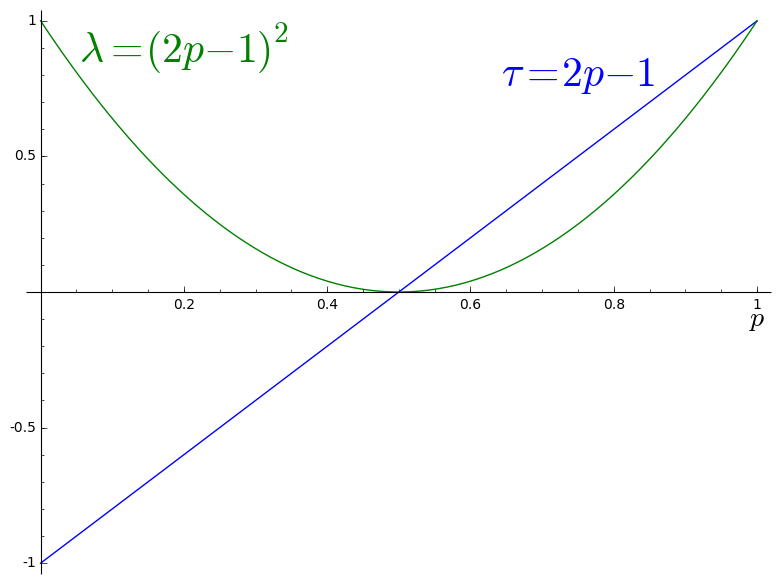
\includegraphics[scale=0.5]{figures/BC_Potenzial2.png}
\end{center}
\caption{The relation between the probability $p$, the
   I/O-correlation\index{I/O-correlation} $\tau$, and the
   potential\index{potential} $\lambda$}\label{fig-bool-pot}
\end{figure}

\begin{sagecode}
\begin{verbatim}

sage: plot1 = plot(2*x-1, (x,0,1))
sage: plot2 = plot((2*x - 1)**2, (x,0,1), color = 'green')
sage: xlabel = text('$p$', (1.0, -0.1), fontsize = 20, color = 'black')
sage: legend1 = text('$\tau = 2p - 1$', (0.75,0.8), fontsize = 30)
sage: legend2 = text('$\lambda = (2p - 1)^2$', (0.2,0.9), fontsize = 30,\\
        color = 'green')
sage: show(plot1 + plot2 + xlabel + legend1 + legend2)
\end{verbatim}
\caption{Plot of I/O-correlation\index{I/O-correlation} and
   potential\index{potential}}\label{Sage-code-bool-pot}
\end{sagecode}

Note that the key $k$ is the target of the attack. As long as it is
unknown, the value of $p_{F,\alpha,\beta,\kappa}(k)$ is also unknown.
Thus for cryptanalysis it makes sense to average the probabilities
of a linear relation over all keys:
\begin{equation}\label{eq-bool-avrg}
   p_{F,\alpha,\beta,\kappa} := \frac{1}{2^{n+l}}
      \#\{(a,k) \in \F_2^n \times \F_2^l \:|\:
           \kappa(k) = \alpha(a) + \beta(F(a,k)) \}.
\end{equation}
This average probability is determined, at least theoretically,
neglecting efficiency, by the definition of the cipher $F$ alone. Calculating
it however amounts to an exhaustion of all plaintexts and keys, and thus
is unrealistic for a realistic cipher with large block lengths.
We extend the definition for the ``average case'' also to
I/O-correlation\index{I/O-correlation} and potential\index{potential}\footnote{%
   Note that the I/O-correlation also is an average, but the potential is not!
}:
\[
   \tau_{F,\alpha,\beta,\kappa} := 2 p_{F,\alpha,\beta,\kappa} - 1,
\]
\[
   \lambda_{F,\alpha,\beta,\kappa} := \tau_{F,\alpha,\beta,\kappa}^2.
\]

Shamir\index{Shamir, Adi}\footnote{%
  Adi Shamir, Israeli cryptologist, co-inventor of the RSA cipher,
  $~^{\ast}$July 6, 1952
}
already in 1985 noticed that the S-boxes of DES\index{DES} admit
linear\index{linear relation}\index{relation!linear} relations with
conspicuous probabilities. However it took another seven years until
Matsui\index{Matsui, Mitsuru}\footnote{%
  Mitsuru Matsui, Japanese cryptologist, $~^{\ast}$September 16, 1961
}
(after first attempts by Gilbert and Chass� 1990 with the cipher FEAL)
succeeded in making systematic use of this observation. For
estimating\index{maximum likelihood estimation}\footnote{%
   This is a maximum likelihood estimation. One decides between
   several hypotheses (two in our case), and prefers the one
   hypothesis that attributes the highest probability to the observation.
}
$\kappa(k)$ he proceeded as follows (in the
case $p_{F,\alpha,\beta,\kappa} > \frac{1}{2}$, else complementary\footnote{%
  In the case $p_{F,\alpha,\beta,\kappa} = \frac{1}{2}$ the method is
  useless.
}):
\begin{enumerate}
   \item {\bf Collect} $N$ pairs of plaintexts and corresponding
      ciphertexts $(a_1,c_1), \ldots, (a_N,c_N)$.

   \item {\bf Count} the number
\[
    t := \# \{i = 1, \ldots, N \:|\: \alpha(a_i) + \beta(c_i) = 0\}.
\]

   \item {\bf Decide} by majority depending on $t$:
	  \begin{itemize}
	    \item If $t > \frac{N}{2}$, estimate $\kappa(k) = 0$.
	    \item If $t < \frac{N}{2}$, estimate $\kappa(k) = 1$.
	  \end{itemize}
\end{enumerate}
The case $t = \frac{N}{2}$ is worthless, however scarce---we might
randomize the decision between $0$ and $1$, or output a suitable
error code\footnote{%
   or both as in SageMath sample~\ref{Sage-code-bool-mats}
}. SageMath sample~\ref{Sage-code-bool-mats}
contains the program code. A concrete application follows as example
in the next subsection.

\begin{sagecode}
\begin{verbatim}

def Matsui_Test(a, b, pc, compl = False):
  """Matsui's test for linear cryptanalysis"""
  N = len(pc)
  results = []
  for pair in pc:
    ax = binScPr(a,pair[0])
    by = binScPr(b,pair[1])
    result = (ax + by) % 2
    results.append(result)
  t = 0
  for bb in results:
    if bb == 0:
      t = t + 1
  if 2*t > N:
    if compl:
      return [t,1,True]
    else:
      return [t,0,True]
  elif 2*t_0 < N:
    if compl:
      return [t,0,True]
    else:
      return [t,1,True]
  else:
    return [t,randint(0,1),False]
\end{verbatim}
\caption{Matsui's test\index{Matsui's test}\index{test!Matsui's}.
   The linear forms are {\tt a}
   for $\alpha$, and {\tt b} for $\beta$. The list {\tt pc} consists of
   {\tt N} pairs of plaintexts and corresponding ciphertexts. The Boolean
   value {\tt compl} indicates if the resulting bit must be inverted.
   The output is a triple consisting of the count {\tt t} of zeros,
   the guessed bit, and the Boolean value that indicates whether the
   bit is deterministic ({\tt True}) or (in the limit case) randomized
   ({\tt False}). We use the function {\tt binScPr} (``binary scalar
   product'') from SageMath sample~\ref{Sage-code-bool-div-bbl} in
   Appendix~\ref{ss-bool-conv}.}\label{Sage-code-bool-mats}
\end{sagecode}

If we detect a linear relation\index{linear relation}\index{relation!linear}
whose probability differs from $\frac{1}{2}$ in a sufficient way, then this
procedure will have a good success probability for sufficiently large $N$.
This allows to reduce the number of unknown key bits by 1, applying
elimination\index{elimination}.

As a theoretical result from these considerations we'll get a connection
between the number $N$ of needed plaintext blocks and the success
probability, see Table~\ref{tab-bool-N}.

The more linear relations with sufficiently high certainty the
attacker finds, the more she can reduce the size of the remaining
key space until finally an exhaustion\index{exhaustion} becomes
feasible. A concrete example in Section~\ref{ss-bool-mini} will
illustrate this.

\subsubsection*{Example}

For a concrete example with $n = l = 4$ we consider the Boolean
map\footnote{%
   By the way $f$ is the S-box\index{S-box} $\mathrm{S}_0$
   of {\sc Lucifer}\index{Lucifer}, a precursor of DES\index{DES}
   developed around 1970.
}
$f$ that is given by the values in Table~\ref{tab-bool-A1}, and
define the bitblock cipher
\[
    F\!: \F_2^4 \times \F_2^4 \longrightarrow \F_2^4 \quad
    \text{by } F(a,k) := f(a + k).
\]
SageMath sample~\ref{Sage-code-Luc-S0} defines this Boolean map
$f =$ {\tt S0}, using the classes {\tt BoolF} and {\tt BoolMap}
from Appendix~\ref{ss-bool-class}.
The columns of the defining matrix (implicit in the SageMath code)
just give the values of the map as they are also found
in the column $y = f(x)$ of Table~\ref{tab-bool-A1}.
(In other words, SageMath sample~\ref{Sage-code-Luc-S0} and
Table~\ref{tab-bool-A1} give equivalent definitions of the map $f$.)
A sample evaluation illustrates this (for the third column,
representing the argument {\tt 0010}).

\begin{sagecode}
\begin{verbatim}

f1 = BoolF([1,1,0,1,1,1,1,0,0,0,0,0,1,0,0,1])
f2 = BoolF([1,1,1,0,1,1,0,0,0,1,0,0,0,1,1,0])
f3 = BoolF([0,1,1,1,1,0,1,0,1,1,1,0,0,0,0,0])
f4 = BoolF([0,1,1,0,0,1,1,0,0,0,1,1,1,0,1,0])
S0 = BoolMap([f1,f2,f3,f4])
# Sample evaluation
sage: S0.valueAt([0,0,1,0])
[0, 1, 1, 1]
\end{verbatim}
\caption{A Boolean map (the S-box $\mathrm{S}_0$ of
   {\sc Lucifer})}\label{Sage-code-Luc-S0}
\end{sagecode}

We encrypt using the key $k = $ \verb:1000: (that we'll attack later as a
test case). For a linear relation we consider the linear forms
\[
     \alpha(a) = a_4, \quad \beta(c) = c_1 + c_2 + c_4, \quad \kappa(k) = k_4.
\]
In Section~\ref{ss-bool-bsp1} we'll see that with these linear forms
the relation $\kappa(k) = \alpha(a) + \beta(c)$ for $F$ has a quite
large probability. Table~\ref{tab-bool-mats} shows the ciphertexts
belonging to three plaintexts $a$ (that later we'll assume as known
plaintexts). The values of $c$ are taken from Table~\ref{tab-bool-A1}.
The number $t$ of observed values $0$ of $\alpha(a)$ + $\beta(c)$
is $t = 2$. Hence the majority decision gives the estimate $k_4 = 0$
(being in cheat mode we know it's correct).

\begin{table}
\begin{center}
\begin{tabular}{|c|c|c|c|} \hline
       $x$   & $y=f(x)$& $\alpha(x) = x_4$ & $\beta(y) = y_1+y_2+y_4$ \\ \hline
     0 0 0 0 & 1 1 0 0 &   0   &  0  \\
     0 0 0 1 & 1 1 1 1 &   1   &  1  \\
     0 0 1 0 & 0 1 1 1 &   0   &  0  \\
     0 0 1 1 & 1 0 1 0 &   1   &  1  \\
     0 1 0 0 & 1 1 1 0 &   0   &  0  \\
     0 1 0 1 & 1 1 0 1 &   1   &  1  \\
     0 1 1 0 & 1 0 1 1 &   0   &  0  \\
     0 1 1 1 & 0 0 0 0 &   1   &  0  \\
     1 0 0 0 & 0 0 1 0 &   0   &  0  \\
     1 0 0 1 & 0 1 1 0 &   1   &  1  \\
     1 0 1 0 & 0 0 1 1 &   0   &  1  \\
     1 0 1 1 & 0 0 0 1 &   1   &  1  \\
     1 1 0 0 & 1 0 0 1 &   0   &  0  \\
     1 1 0 1 & 0 1 0 0 &   1   &  1  \\
     1 1 1 0 & 0 1 0 1 &   0   &  0  \\
     1 1 1 1 & 1 0 0 0 &   1   &  1  \\ \hline
\end{tabular}
\end{center}
\caption{Value table of a Boolean map
  $f\!: \F_2^4 \longrightarrow \F_2^4$, and two linear forms}\label{tab-bool-A1}
\end{table}

\begin{table}
\begin{center}
\begin{tabular}{|c|c|c||ccc|}\hline
   $a$  & $a+k$ & $c$  & $\alpha(a)$ & $\beta(c)$ & $\alpha(a)$ + $\beta(c)$ \\
   \hline
   0010 & 1010  & 0011 &     0       &      1     &             1            \\
   0101 & 1101  & 0100 &     1       &      1     &             0            \\
   1010 & 0010  & 0111 &     0       &      0     &             0            \\
   \hline
\end{tabular}
\end{center}
\caption{Estimating a key bit after Matsui using three known
   plaintexts}\label{tab-bool-mats}
\end{table}

This was easily done with pencil and paper. However it might be instructive
to retrace the count in SageMath for a better understanding of more complex examples.
SageMath sample~\ref{Sage-code-Mats-Expl} provides this. It uses the function
{\tt xor} from SageMath sample~\ref{Sage-code-bool-div-bbl} in Appendix~\ref{ss-bool-conv},
as well {\tt S0} from SageMath sample~\ref{Sage-code-Luc-S0}. The result
\mbox{\tt [2, 0, True]} says that we found $2$ zeroes among the counted values,
yielding the majority decision $0$, and the output parameter {\tt True} tells
that the decision was deterministic, not randomized.

\begin{sagecode}
\begin{verbatim}

sage: k = [1,0,0,0]
sage: alpha = [0,0,0,1]
sage: beta = [1,1,0,1]
sage: plist = [[0,0,1,0],[0,1,0,1],[1,0,1,0]]
sage: xlist = []
sage: xclist = []
sage: pclist = []
sage: for i in range(0,len(plist)):
....:     x = xor(plist[i],k)
....:     xlist.append(x)
....:     
sage: xlist
[[1, 0, 1, 0], [1, 1, 0, 1], [0, 0, 1, 0]]
sage: for i in range(0,len(plist)):
....:     val = S0.valueAt(xlist[i])
....:     xclist.append([xlist[i],val])
....:     pclist.append([plist[i],val])
....:     
sage: Matsui_Test(alpha,beta,pclist,False)
[2, 0, True]
\end{verbatim}
\caption{An example of Matsui's test\index{Matsui's test}}\label{Sage-code-Mats-Expl}
\end{sagecode}

\noindent How successful will this procedure be in general? We have to analyse the problems:
\begin{enumerate}
	\item How to find linear\index{linear relation}\index{relation!linear}
        relations of sufficiently high probabilities?
     \item Since in general bitblock\index{bitblock cipher} ciphers consist of
        several rounds\index{round} we ask:
	\begin{enumerate}
	  \item How to find useful linear relations for the round function of an
          iterated bitblock cipher?
	  \item How to combine these over the rounds as a linear relation for the
          complete cipher?
	  \item How to calculate the probability of a combined linear relation for
          the complete cipher from the probabilities for the single rounds?
	\end{enumerate}
\end{enumerate}

\noindent The answer to the first question and part (a) of the second one is: from the
linear\index{linear profile}\index{profile!linear} profile, see
Section~\ref{ss-bool-lpr}. The following partial questions lead to the
analysis of linear paths\index{linear path}\index{path!linear}, see
Section~\ref{ss-bool-path}, and the cumulation of probabilities, see
Theorem~\ref{thm-bool-rrnd}. For (c) finally we'll find a useful rule of thumb.

\subsection{Example A: A One-Round Cipher}\label{ss-bool-bsp1}

We consider examples that are much too simple for real
world applications but illustrate the principles of
linear\index{linear cryptanalysis}\index{cryptanalysis!linear}
cryptanalysis in an easily intelligible way. We always assume round
functions of the type $f(a+k)$, that is we add the key---or
an $n$-bit part of it---to the plaintext\footnote{%
   This is a quite special method of bringing the key into
   play but nevertheless realistic. The paradigmatic
   sample ciphers {\sc Lucifer}\index{Lucifer}, DES\index{DES},
   and AES\index{AES} do so. The term used with AES \cite{DaRi}
   is ``key-alternating cipher structure''.
} before applying a bijective
S-box $f\!: \F_2^n \longrightarrow \F_2^n$. The simplest model is
encryption by the formula
\[
   c = f(a+k),
\]
see\footnote{%
  The graphics here and later represent the map $f$ sometimes by the
  S-box S in the elementwise assignments.
} Figure~\ref{fig-bool-bsp0}.
This example is pointless because one block of known
plaintext\index{known plaintext}\index{plaintext!known} gives
a solution\footnote{%
   We assume that the attacker knows the inverse map $f^{-1}$ that
   is part of the decryption algorithm. One-way\index{one-way encryption}
   encryption methods that assume that $f^{-1}$ is not efficiently
   deducible from $f$ are the subject of another part of cryptography.
} for $k$:
\[
   k = f^{-1}(c) + a.
\]

\begin{figure}
\begin{center}
\begin{picture}(268,68)(0,0)
% Mengen
   \put(11,14){$\F_2^n$}
   \put(28,17){\vector(1,0){34}}
   \put(66,14){$\F_2^n$}
   \put(54,26){$\bigoplus$}
   \put(66,54){$\F_2^n$}
   \put(71,51){\vector(0,-1){28}}
   \put(83,17){\vector(1,0){34}}
   \put(94,20){$f$}
   \put(123,14){$\F_2^n$}

% Elemente
   \put(154,14){$a$}
   \put(165,17){\vector(1,0){28}}
   \put(165,14){\line(0,1){6}}
   \put(197,14){$b$}
   \put(197,54){$k$}
   \put(199,51){\vector(0,-1){28}}
   \put(197,51){\line(1,0){6}}
   \put(205,17){\vector(1,0){40}}
   \put(205,14){\line(0,1){6}}
   \put(214,14){\fcolorbox{black}{yellow}{S}}
   \put(251,14){$c$}

% Rahmen
   \put(0,0){\line(1,0){268}}
   \put(0,68){\line(1,0){268}}
   \put(0,0){\line(0,1){68}}
   \put(268,0){\line(0,1){68}}
\end{picture}
\end{center}
\caption{A (much too) simple example}\label{fig-bool-bsp0}
\end{figure}

\begin{figure}
\begin{center}
\begin{picture}(208,137)(0,0)
% Mengen
   \put(11,83){$\F_2^n$}
   \put(28,85){\vector(1,0){34}}
   \put(66,83){$\F_2^n$}
   \put(54,94){$\bigoplus$}
   \put(66,124){$\F_2^n$}
   \put(71,120){\vector(0,-1){28}}
   \put(83,85){\vector(1,0){34}}
   \put(94,88){$f$}
   \put(125,83){$\F_2^n$}
   \put(140,85){\vector(1,0){34}}
   \put(179,124){$\F_2^n$}
   \put(185,120){\vector(0,-1){28}}
   \put(168,94){$\bigoplus$}
   \put(179,83){$\F_2^n$}

% Elemente
   \put(23,14){$a$}
   \put(34,17){\vector(1,0){28}}
   \put(34,14){\line(0,1){6}}
   \put(71,14){$b$}
   \put(68,54){$k^{(0)}$}
   \put(74,51){\vector(0,-1){28}}
   \put(71,51){\line(1,0){6}}
   \put(80,17){\vector(1,0){40}}
   \put(80,14){\line(0,1){6}}
   \put(91,14){\fcolorbox{black}{yellow}{S}}
   \put(128,14){$b'$}
   \put(179,54){$k^{(1)}$}
   \put(185,51){\vector(0,-1){28}}
   \put(182,51){\line(1,0){6}}
   \put(142,17){\vector(1,0){28}}
   \put(142,14){\line(0,1){6}}
   \put(182,14){$c$}

% Rahmen
   \put(0,0){\line(1,0){208}}
   \put(0,137){\line(1,0){208}}
   \put(0,0){\line(0,1){137}}
   \put(208,0){\line(0,1){137}}
\end{picture}
\end{center}
\caption{Example A: A One-Round Cipher}\label{fig-bool-bspA}
\end{figure}

\begin{figure}
\begin{center}
\begin{picture}(85,68)(0,0)
   \put(6,48){$\F_2^n$}
   \put(23,51){\vector(1,0){40}}
   \put(40,54){$f$}
   \put(68,48){$\F_2^n$}
   \put(40,9){$\F_2$}
   \put(17,43){\vector(1,-1){23}}
   \put(17,26){$\alpha$}
   \put(68,43){\vector(-1,-1){23}}
   \put(60,26){$\beta$}
   \put(38,31){$\stackrel{p}{\approx}$}

% Rahmen
   \put(0,0){\line(1,0){85}}
   \put(0,68){\line(1,0){85}}
   \put(0,0){\line(0,1){68}}
   \put(85,0){\line(0,1){68}}
\end{picture}
\end{center}
\caption{Diagram for an ``approximative'' linear
   relation\index{linear relation}\index{relation!linear}}\label{fig-bool-appr}
\end{figure}

The somewhat more involved example A stops this attack:
\[
   c = f(a+k^{(0)}) + k^{(1)}
\]
(see Figure~\ref{fig-bool-bspA}). This is the simplest example for which
the method of
linear cryptanalysis\index{linear cryptanalysis}\index{cryptanalysis!linear}
makes sense: Let $(\alpha,\beta)$ be a pair of linear\index{linear form}
forms with
\begin{equation}\label{eq-bool-prob}
     \beta\circ f(x) \stackrel{p}{\approx} \alpha(x),
\end{equation}
where the symbol $\stackrel{p}{\approx}$ reads as ``equal with
probability $p$'', or in other words
\[
     p = p_{f,\alpha,\beta} :=
     \frac{1}{2^{n}} \cdot \#\{x \in \F_2^n \:|\: \beta\circ f(x) = \alpha(x) \}.
\]
The diagram in Figure~\ref{fig-bool-appr} illustrates Formula~(\ref{eq-bool-prob}).
Note that the linear form $\kappa$ of the general theory is implicit
in the present context: Since the key bits are simply added to plaintext
and (``intermediary'') ciphertext we have $\kappa = \alpha$ for $k^{(0)}$,
and $\kappa = \beta$ for $k^{(1)}$, hence
$\kappa(k^{(0)}, k^{(1)}) = \alpha(k^{(0)}) + \beta(k^{(1)})$.

How does this scenario fit the general situation from Section~\ref{ss-bool-lka}?
In example~A we have
\begin{itemize}
   \item key length $l = 2n$, key space $\F_2^{2n}$, and
      keys of the form $k = (k^{(0)},k^{(1)})$ with $k^{(0)}, k^{(1)} \in \F_2^n$.
   \item The cipher is defined by the map
\[
     F\!: \F_2^n \times \F_2^n \times \F_2^n \longrightarrow \F_2^n,
     \quad (a, k^{(0)}, k^{(1)}) \mapsto f(a + k^{(0)}) + k^{(1)}.
\]
   \item The linear form $\kappa\!: \F_2^n \times \F_2^n \longrightarrow \F_2$
      is $\kappa(k^{(0)},k^{(1)}) = \alpha(k^{(0)}) + \beta(k^{(1)})$.
\end{itemize}
Hence the probability of a linear relation for a fixed key
\mbox{$k = (k^{(0)},k^{(1)})$} is
\begin{eqnarray*}
    p_{F,\alpha,\beta,\kappa}(k) & = & \frac{1}{2^n} \cdot
      \#\{a \in \F_2^n \:|\: \kappa(k) = \alpha(a) + \beta(F(a,k)) \} \\
     & = & \frac{1}{2^n} \cdot
      \#\{a \in \F_2^n \:|\: \alpha(k^{(0)}) + \beta(k^{(1)}) = \alpha(a) + \beta(f(a + k^{(0)}) + k^{(1)}) \} \\
     & = & \frac{1}{2^n} \cdot
      \#\{a \in \F_2^n \:|\: \alpha(k^{(0)}) = \alpha(a) + \beta(f(a + k^{(0)})) \},
\end{eqnarray*}
where we omitted $\beta(k^{(1)})$ that occurs on both sides of the equation
inside the curly set brackets.

This expression is independent of $k^{(1)}$, and the slightly rewritten
equation
\[
     p_{F,\alpha,\beta,\kappa}(k) = \frac{1}{2^n} \cdot
      \#\{a \in \F_2^n \:|\: \alpha(a + k^{(0)}) = \beta(f(a + k^{(0)})) \}
\]
shows that it assumes the same value for all $k^{(0)}$: With $a$ also
$a + k^{(0)}$ runs through all of $\F_2^n$ for a fixed $k^{(0)}$.
Therefore this value must agree with the mean value over all $k$:
\[
     p_{F,\alpha,\beta,\kappa}(k) = p_{F,\alpha,\beta,\kappa} = \frac{1}{2^n} \cdot
      \#\{x \in \F_2^n \:|\: \alpha(x) = \beta(f(x)) \} = p.
\]
This consideration shows:

\begin{theorem}
    In the scenario of example~A the probability $p_{F,\alpha,\beta,\kappa}(k)$
    assumes the same value
\[
     p = \frac{1}{2^n} \cdot \#\{x \in \F_2^n \:|\: \alpha(x) = \beta(f(x)) \}
\]
   for all keys $k \in \F_2^{2n}$. In particular $p$ coincides with the mean value
   from Equation~{\rm (\ref{eq-bool-avrg})}.
\end{theorem}

Using the notations from Figure~\ref{fig-bool-bspA} we have
\begin{align*}
   \beta(c) & = \beta(b' + k^{(1)}) = \beta(b') + \beta(k^{(1)}) \\
            & \stackrel{p}{\approx} \alpha(b) + \beta(k^{(1)})
                   = \alpha(a + k^{(0)}) + \beta(k^{(1)})
                        = \alpha(a) + \alpha(k^{(0)}) + \beta(k^{(1)}).
\end{align*}
This yields a linear\index{linear relation}\index{relation!linear}
relation for the bits of the key $k = (k_1,k_2)$:
\[
   \alpha(k^{(0)}) + \beta(k^{(1)}) \stackrel{p}{\approx} \alpha(a) + \beta(c).
\]
Treating the complementary relation
\[
   \beta\circ f(x) \stackrel{1-p}{\approx} \alpha(x) + 1
\]
in an analoguous way we get:

\begin{theorem}
   In the scenario of example A let $(\alpha,\beta)$ be a pair of
   linear\index{linear form} forms for $f$ with probability $p$ as in
   Formula~{\rm (\ref{eq-bool-prob})}.
   Then $\hat{p} = \max\{p, 1-p\}$ is the success probability
   for determing a single key bit by this linear
   relation\index{linear relation}\index{relation!linear} given
   {\em one} known\index{known plaintext}\index{plaintext!known}
   plaintext block.
\end{theorem}

\subsubsection*{Example}

Take $n = 4$, and for $f$ take the S-box
$\mathrm{S}_0$ of {\sc Lucifer}\index{Lucifer}. As the two rightmost
columns of Table~\ref{tab-bool-A1} show the linear relation defined
by $(\alpha,\beta)$, where $\alpha(x) = x_4$ and $\beta(y) = y_1+y_2+y_4$,
has probability\footnote{%
   providing strong evidence that the designers of {\sc Lucifer}\index{Lucifer}
   weren't aware of linear\index{linear cryptanalysis}\index{cryptanalysis!linear}
   cryptanalysis
} $p_{f,\alpha,\beta} = \frac{14}{16} = \frac{7}{8}$.

As concrete round\index{round key} keys take $k_0 = $\verb:1000: and $k_1 = $\verb:0001:.
Table~\ref{tab-bool-linrel}, running through all possible $16$ plaintexts,
shows that $\alpha(a)+\beta(c)$ assumes the value $1 =\alpha(k_0) + \beta(k_1)$
for this partial sum of key bits exactly $14$ times---as expected.

\begin{table}
\begin{center}
\begin{tabular}{|cccc|c|} \hline
  $a$  & $b$  & $b'$ & $c$  & $\alpha(a)+\beta(c)$ \\ \hline
  0000 & 1000 & 0010 & 0011 & 1 \\
  0001 & 1001 & 0110 & 0111 & 1 \\
  0010 & 1010 & 0011 & 0010 & 0 \\
  0011 & 1011 & 0001 & 0000 & 1 \\
  0100 & 1100 & 1001 & 1000 & 1 \\
  0101 & 1101 & 0100 & 0101 & 1 \\
  0110 & 1110 & 0101 & 0100 & 1 \\
  0111 & 1111 & 1000 & 1001 & 1 \\
  1000 & 0000 & 1100 & 1101 & 1 \\
  1001 & 0001 & 1111 & 1110 & 1 \\
  1010 & 0010 & 0111 & 0110 & 1 \\
  1011 & 0011 & 1010 & 1011 & 1 \\
  1100 & 0100 & 1110 & 1111 & 1 \\
  1101 & 0101 & 1101 & 1100 & 1 \\
  1110 & 0110 & 1011 & 1010 & 1 \\
  1111 & 0111 & 0000 & 0001 & 0 \\
  \hline
\end{tabular}
\end{center}
\caption{A linear relation for the key bits ($b$ arises from $a$ by adding
   $k^{(0)}$, resulting in ``flipping'' the first bit, $b'$ from $b$ by applying
   $f$, and $c$ from $b'$ by adding $k^{(1)}$.}\label{tab-bool-linrel}
\end{table}

How large is the success probability $p_N$ of correctly estimating
this partial sum, assuming $N = 1, 2, \ldots$ random
known\index{known plaintext}\index{plaintext!known} plaintexts
from the set of $2^n$ possible plaintexts? (For given linear forms
$\alpha$ and $\beta$ with $p = p_{f,\alpha,\beta}$.) This is
exactly the scenario of the hypergeometric
distribution\index{hypergeometric distribution}\index{distribution!hypergeometric}\footnote{%
   that we won't explain here
}.
Therefore we have:

\begin{theorem}
  In example A let $(\alpha,\beta)$ be a pair of linear forms that
  defines a linear relation for $f$ with probability $p$.
  Then the success probability for determining a key bit by this linear
  relation\index{linear relation}\index{relation!linear} from $N$ known
  plaintexts is the cumulated probability $p_N = p_N^{(s)}$ of the
  hypergeometric distribution with parameters $2^n$,
  $s = \hat{p}\cdot 2^n$, and $N$ where $\hat{p} = \max\{p, 1-p\}$.
\end{theorem}

If we neglect exact mathematical reasoning and work with asymptotic
approximations (as is common in applied statistics), then we can
replace the hypergeometric
distribution\index{hypergeometric distribution}\index{distribution!hypergeometric}
by the normal distribution\index{normal distribution}\index{distribution!normal}.
The usual (quite vaguely stated) conditions for this approximation are ``$p$ not too
different from $\frac{1}{2}$, $N \ll 2^n$, but $N$ not too small.''
This gives the formula
\begin{equation}\label{equ-bool-N}
  p_N \approx \frac{1}{\sqrt{2\pi}} \cdot
                      \int_{-\infty}^{\sqrt{N\lambda}} e^{-t^2/2}\,dt,
\end{equation}
where $\lambda = (2p - 1)^2$ is the potential\index{potential} of the
linear relation. The values associated with the normal distribution\footnote{%
   Instead of the approximation by the normal distribution we could
   directly use the hypergeometric
   distribution\index{hypergeometric distribution}\index{distribution!hypergeometric}.
   This would, in particular for small $N$, give a more precise value
   but not a closed formula as simple as (\ref{equ-bool-N}).
} are well-known
and yield Table~\ref{tab-bool-N}. To get a success probability of
about $95\%$ we need $N \approx \frac{3}{\lambda}$ known
plaintexts\index{known plaintext}\index{plaintext!known}
according to the table. In the concrete example above
we had $p = \frac{7}{8}$, hence $\lambda = \frac{9}{16}$,
and the number of known plaintexts needed for a $95\%$
success probability is $N \approx 5$. Using Table~\ref{tab-bool-mats}
we succeeded with only $N = 3$ plaintexts. This is no great surprise
because the a-priori probability of this success is about 90\% (for
$N\lambda = \frac{27}{16} \approx 1,68\ldots$)\footnote{%
   Here the condition ``$N$ not too small'' for the approximation by the
   normal distribution\index{normal distribution}\index{distribution!normal}
   is more than arguable. However determining the exact values for the hypergeometric
   distribution\index{hypergeometric distribution}\index{distribution!hypergeometric}
   is easy:
   Consider an urn containing $16$ balls, $14$ black ones and
   $2$ white ones, and draw $3$ balls by random. Then the probability of all
   of them being black is $\frac{26}{40}$, the probability of two being black
   and one being white is $\frac{13}{40}$. Hence the probability of at least
   two balls being black is $\frac{39}{40} = 97,5\%$. This is clearly more
   than the 90\% from the approximation~(\ref{equ-bool-N}).
   The remaining probabilities are $\frac{1}{40}$ for exactly one black
   ball, and $0$ for three white balls.
}.

\begin{table}
\begin{center}
  \begin{tabular}{|c|ccccccc|} \hline
		$N\lambda$ & $1$ & $2$ & $3$ & $4$ & \ldots & $8$ & $9$ \\
		$p_N$ & $84,1\%$ & $92,1\%$ & $95,8\%$ & $97,7\%$ & \ldots &
		                      $99,8\%$ & $99,9\%$ \\ \hline
  \end{tabular}
\end{center}
\caption{Dependence of the success probability on the number of known
   plaintexts\index{known plaintext}\index{plaintext!known}}\label{tab-bool-N}
\end{table}

\subsection{Approximation Table\index{approximation table},
   Correlation Matrix\index{correlation matrix}, and Linear
   Profile\index{linear profile}\index{profile!linear}}\label{ss-bool-lpr}

Linear relations\index{linear relation}\index{relation!linear} for a Boolean
map\index{Boolean map}\index{map!Boolean} (or S-box\index{S-box})
$f\!\!: \F_2^n \longrightarrow \F_2^q$ are true with certain frequencies
(or probabilities). We collect these frequencies in a matrix of size
$2^n \times 2^q$, called the
{\bf approximation table\index{approximation table}}\footnote{%
   When using references be aware that often all entries are diminished
   by $2^{n-1}$, for example by the SageMath function
   {\tt linear\_approximation\_matrix()}.
}\label{fn-lin-appr}
of $f$. This table gives, for each pair $(\alpha,\beta)$ of linear
forms\index{linear form}, the number of arguments $x$ where
\mbox{$\beta\circ f(x) = \alpha(x)$.}
Table~\ref{tab-bool-s0} shows the approximation table of the S-box $\mathrm{S}_0$
of {\sc Lucifer}\index{Lucifer}. The entry $16$ in the upper left corner
says that the relation $0 = 0$ is true in all $16$
possible cases. At the same time $16$ is the common denominator by which
we have to divide all other entries to get the probabilities. In the general case
the upper left corner would be  $2^n$. The remaining entries of the first column
(corresponding to $\beta = 0$) are $8$ because each non-zero
linear form\index{linear form} $\alpha$ takes the value $0$ in exactly half
of all cases, that is $8$ times\footnote{%
   In the language of linear algebra\index{linear algebra}\index{algebra!linear}
   we express this fact as:
   The kernel of a linear form\index{linear form} $\neq 0$ is a subspace of
   dimension $n-1$.
}. For the first row an analogous argument is true---provided that $f$ is
bijective\footnote{%
   In the general case where $q$ could be $\neq n$ we would use the concept
   ``balanced\index{balanced}'' that means that all preimages have the same
   size. Of course a map can be balanced only in the case $q \leq n$.
}.

\begin{table}
\begin{center}
\begin{tabular}{|c|cccccccccccccccc|} \hline
     & 0 & 1 & 2 & 3 & 4 & 5 & 6 & 7 & 8 & 9 &10 &11 &12 &13 &14 &15 \\ \hline
   0 &16 & 8 & 8 & 8 & 8 & 8 & 8 & 8 & 8 & 8 & 8 & 8 & 8 & 8 & 8 & 8 \\
   1 & 8 & 6 & 6 & 8 & 8 & 6 & 6 & 8 & 8 & 6 & 6 & 8 & 8 &14 & 6 & 8 \\
   2 & 8 &10 & 8 & 6 & 4 & 6 & 8 & 6 & 6 &12 & 6 & 8 &10 & 8 & 6 & 8 \\
   3 & 8 &12 &10 & 6 &12 & 8 &10 & 6 & 6 & 6 & 8 & 8 &10 &10 & 8 & 8 \\
   4 & 8 & 8 & 4 & 8 & 8 & 8 & 8 & 4 &10 & 6 & 6 & 6 &10 & 6 &10 &10 \\
   5 & 8 &10 &10 &12 & 8 &10 & 6 & 8 &10 & 8 & 4 &10 &10 & 8 & 8 & 6 \\
   6 & 8 &10 & 8 &10 & 8 &10 & 8 &10 & 8 &10 & 8 & 2 & 8 &10 & 8 &10 \\
   7 & 8 & 8 &10 & 6 & 8 & 8 & 2 & 6 & 8 & 8 &10 & 6 & 8 & 8 &10 & 6 \\
   8 & 8 & 8 & 6 &10 & 6 &10 & 8 & 8 & 4 & 8 &10 &10 &10 &10 &12 & 8 \\
   9 & 8 &10 & 8 &10 & 6 & 4 &10 & 8 & 8 & 6 & 8 & 6 & 6 & 8 &10 & 4 \\
  10 & 8 & 6 &10 & 8 & 6 & 8 & 8 &10 & 6 & 4 & 8 & 6 &12 & 6 & 6 & 8 \\
  11 & 8 &12 & 8 & 8 & 6 & 6 & 6 &10 &10 & 6 &10 &10 & 8 & 8 & 8 &12 \\
  12 & 8 & 8 &10 &10 & 6 &10 & 8 & 4 & 6 & 6 & 8 & 8 & 4 & 8 & 6 &10 \\
  13 & 8 & 6 &12 & 6 & 6 & 8 &10 & 8 &10 & 8 & 6 & 8 & 8 &10 &12 & 8 \\
  14 & 8 & 6 &10 &12 &10 & 4 & 8 & 6 & 8 &10 &10 & 8 &10 & 8 & 8 &10 \\
  15 & 8 & 8 & 8 & 8 &10 & 6 & 6 &10 & 4 & 8 & 4 & 8 & 6 & 6 &10 &10 \\ \hline
\end{tabular}
\end{center}
\caption{Approximation table of the S-box $\mathrm{S}_0$ of {\sc Lucifer}\index{Lucifer}.
   Row and column indices are linear forms represented by integers,
   see Section~\ref{ss-bool-repr}.
   To get the probabilities divide by 16.}\label{tab-bool-s0}
\end{table}

\begin{table}
\begin{center}
\begin{tabular}{|c|cccccccccccccccc|} \hline
     & 0 & 1 & 2 & 3 & 4 & 5 & 6 & 7 & 8 & 9 &10 &11 &12 &13 &14 &15 \\ \hline
   0 & 1 & 0 & 0 & 0 & 0 & 0 & 0 & 0 & 0 & 0 & 0 & 0 & 0 & 0 & 0 & 0 \\
   1 & 0 &$-\frac{1}{4}$&$-\frac{1}{4}$& 0 & 0 &$-\frac{1}{4}$&$-\frac{1}{4}$& 0 & 0 &$-\frac{1}{4}$&$-\frac{1}{4}$& 0 & 0 &$\frac{3}{4}$&$-\frac{1}{4}$& 0 \\
   2 & 0 &$\frac{1}{4}$& 0 & $-\frac{1}{4}$ &$-\frac{1}{2}$& $-\frac{1}{4}$ & 0 & $-\frac{1}{4}$ & $-\frac{1}{4}$ &$\frac{1}{2}$& $-\frac{1}{4}$ & 0 &$\frac{1}{4}$& 0 & $-\frac{1}{4}$ & 0 \\
   3 & 0 &$\frac{1}{2}$&$\frac{1}{4}$& $-\frac{1}{4}$ &$\frac{1}{2}$& 0 &$\frac{1}{4}$& $-\frac{1}{4}$ & $-\frac{1}{4}$ & $-\frac{1}{4}$ & 0 & 0 &$\frac{1}{4}$&$\frac{1}{4}$& 0 & 0 \\
   4 & 0 & 0 &$-\frac{1}{2}$& 0 & 0 & 0 & 0 &$-\frac{1}{2}$&$\frac{1}{4}$& $-\frac{1}{4}$ & $-\frac{1}{4}$ & $-\frac{1}{4}$ &$\frac{1}{4}$& $-\frac{1}{4}$ &$\frac{1}{4}$&$\frac{1}{4}$\\
   5 & 0 &$\frac{1}{4}$&$\frac{1}{4}$&$\frac{1}{2}$& 0 &$\frac{1}{4}$& $-\frac{1}{4}$ & 0 &$\frac{1}{4}$& 0 &$-\frac{1}{2}$&$\frac{1}{4}$&$\frac{1}{4}$& 0 & 0 & $-\frac{1}{4}$ \\
   6 & 0 &$\frac{1}{4}$& 0 &$\frac{1}{4}$& 0 &$\frac{1}{4}$& 0 &$\frac{1}{4}$& 0 &$\frac{1}{4}$& 0 &$-\frac{3}{4}$& 0 &$\frac{1}{4}$& 0 &$\frac{1}{4}$\\
   7 & 0 & 0 &$\frac{1}{4}$& $-\frac{1}{4}$ & 0 & 0 &$-\frac{3}{4}$& $-\frac{1}{4}$ & 0 & 0 &$\frac{1}{4}$& $-\frac{1}{4}$ & 0 & 0 &$\frac{1}{4}$& $-\frac{1}{4}$ \\
   8 & 0 & 0 & $-\frac{1}{4}$ &$\frac{1}{4}$& $-\frac{1}{4}$ &$\frac{1}{4}$& 0 & 0 &$-\frac{1}{2}$& 0 &$\frac{1}{4}$&$\frac{1}{4}$&$\frac{1}{4}$&$\frac{1}{4}$&$\frac{1}{2}$& 0 \\
   9 & 0 &$\frac{1}{4}$& 0 &$\frac{1}{4}$& $-\frac{1}{4}$ &$-\frac{1}{2}$&$\frac{1}{4}$& 0 & 0 & $-\frac{1}{4}$ & 0 & $-\frac{1}{4}$ & $-\frac{1}{4}$ & 0 &$\frac{1}{4}$&$-\frac{1}{2}$\\
  10 & 0 & $-\frac{1}{4}$ &$\frac{1}{4}$& 0 & $-\frac{1}{4}$ & 0 & 0 &$\frac{1}{4}$& $-\frac{1}{4}$ &$-\frac{1}{2}$& 0 & $-\frac{1}{4}$ &$\frac{1}{2}$& $-\frac{1}{4}$ & $-\frac{1}{4}$ & 0 \\
  11 & 0 &$\frac{1}{2}$& 0 & 0 & $-\frac{1}{4}$ & $-\frac{1}{4}$ & $-\frac{1}{4}$ &$\frac{1}{4}$&$\frac{1}{4}$& $-\frac{1}{4}$ &$\frac{1}{4}$&$\frac{1}{4}$& 0 & 0 & 0 &$\frac{1}{2}$\\
  12 & 0 & 0 &$\frac{1}{4}$&$\frac{1}{4}$& $-\frac{1}{4}$ &$\frac{1}{4}$& 0 &$-\frac{1}{2}$& $-\frac{1}{4}$ & $-\frac{1}{4}$ & 0 & 0 &$-\frac{1}{2}$& 0 & $-\frac{1}{4}$ &$\frac{1}{4}$\\
  13 & 0 & $-\frac{1}{4}$ &$\frac{1}{2}$& $-\frac{1}{4}$ & $-\frac{1}{4}$ & 0 &$\frac{1}{4}$& 0 &$\frac{1}{4}$& 0 & $-\frac{1}{4}$ & 0 & 0 &$\frac{1}{4}$&$\frac{1}{2}$& 0 \\
  14 & 0 & $-\frac{1}{4}$ &$\frac{1}{4}$&$\frac{1}{2}$&$\frac{1}{4}$&$-\frac{1}{2}$& 0 & $-\frac{1}{4}$ & 0 &$\frac{1}{4}$&$\frac{1}{4}$& 0 &$\frac{1}{4}$& 0 & 0 &$\frac{1}{4}$\\
  15 & 0 & 0 & 0 & 0 &$\frac{1}{4}$& $-\frac{1}{4}$ & $-\frac{1}{4}$ &$\frac{1}{4}$&$-\frac{1}{2}$& 0 &$-\frac{1}{2}$& 0 & $-\frac{1}{4}$ & $-\frac{1}{4}$ &$\frac{1}{4}$&$\frac{1}{4}$\\ \hline
\end{tabular}
\end{center}\caption{Correlation matrix of the S-box $\mathrm{S}_0$ of {\sc Lucifer}\index{Lucifer}.
   Row and column indices are linear forms represented by integers.}\label{tab-bool-corr}
\end{table}

\begin{table}
\begin{center}
\begin{tabular}{|c|cccccccccccccccc|} \hline
  &0& 1            & 2            & 3            & 4            & 5            & 6            & 7            
     & 8            & 9            &10            &11            &12            &13            &14            &15            \\
\hline
 0&1& 0            & 0            & 0            & 0            & 0            & 0            & 0            
     & 0            & 0            & 0            & 0            & 0            & 0            & 0            & 0            \\
 1&0&$\frac{1}{16}$&$\frac{1}{16}$& 0            & 0            &$\frac{1}{16}$&$\frac{1}{16}$& 0            
     & 0            &$\frac{1}{16}$&$\frac{1}{16}$& 0            & 0            &$\frac{9}{16}$&$\frac{1}{16}$& 0            \\
 2&0&$\frac{1}{16}$& 0            &$\frac{1}{16}$&$\frac{1}{4}$ &$\frac{1}{16}$& 0            &$\frac{1}{16}$&$\frac{1}{16}$
     &$\frac{1}{4}$ &$\frac{1}{16}$& 0            &$\frac{1}{16}$& 0            &$\frac{1}{16}$& 0            \\
 3&0&$\frac{1}{4}$ &$\frac{1}{16}$&$\frac{1}{16}$&$\frac{1}{4}$ & 0            &$\frac{1}{16}$&$\frac{1}{16}$&$\frac{1}{16}$
     &$\frac{1}{16}$& 0            & 0            &$\frac{1}{16}$&$\frac{1}{16}$& 0            & 0            \\
 4&0& 0            &$\frac{1}{4}$ & 0            & 0            & 0            & 0            &$\frac{1}{4}$ &$\frac{1}{16}$
     &$\frac{1}{16}$&$\frac{1}{16}$&$\frac{1}{16}$&$\frac{1}{16}$&$\frac{1}{16}$&$\frac{1}{16}$&$\frac{1}{16}$\\
 5&0&$\frac{1}{16}$&$\frac{1}{16}$&$\frac{1}{4}$ & 0            &$\frac{1}{16}$&$\frac{1}{16}$& 0            &$\frac{1}{16}$
     & 0            &$\frac{1}{4}$ &$\frac{1}{16}$&$\frac{1}{16}$& 0            & 0            &$\frac{1}{16}$\\
 6&0&$\frac{1}{16}$& 0            &$\frac{1}{16}$& 0            &$\frac{1}{16}$& 0            &$\frac{1}{16}$& 0            
     &$\frac{1}{16}$& 0            &$\frac{9}{16}$& 0            &$\frac{1}{16}$& 0            &$\frac{1}{16}$\\
 7&0& 0            &$\frac{1}{16}$&$\frac{1}{16}$& 0            & 0            &$\frac{9}{16}$&$\frac{1}{16}$& 0            
     & 0            &$\frac{1}{16}$&$\frac{1}{16}$& 0            & 0            &$\frac{1}{16}$&$\frac{1}{16}$\\
 8&0& 0            &$\frac{1}{16}$&$\frac{1}{16}$&$\frac{1}{16}$&$\frac{1}{16}$& 0            & 0            &$\frac{1}{4}$ 
     & 0            &$\frac{1}{16}$&$\frac{1}{16}$&$\frac{1}{16}$&$\frac{1}{16}$&$\frac{1}{4}$ & 0            \\
 9&0&$\frac{1}{16}$& 0            &$\frac{1}{16}$&$\frac{1}{16}$&$\frac{1}{4}$&$\frac{1}{16}$& 0            & 0            
     &$\frac{1}{16}$& 0            &$\frac{1}{16}$&$\frac{1}{16}$& 0            &$\frac{1}{16}$&$\frac{1}{4}$ \\
10&0&$\frac{1}{16}$&$\frac{1}{16}$& 0            &$\frac{1}{16}$& 0            & 0            &$\frac{1}{16}$&$\frac{1}{16}$
     &$\frac{1}{4}$ & 0            &$\frac{1}{16}$&$\frac{1}{4}$ &$\frac{1}{16}$&$\frac{1}{16}$& 0            \\
11&0&$\frac{1}{4}$ & 0            & 0            &$\frac{1}{16}$&$\frac{1}{16}$&$\frac{1}{16}$&$\frac{1}{16}$&$\frac{1}{16}$
     &$\frac{1}{16}$&$\frac{1}{16}$&$\frac{1}{16}$& 0            & 0            & 0            &$\frac{1}{4}$ \\
12&0& 0            &$\frac{1}{16}$&$\frac{1}{16}$&$\frac{1}{16}$&$\frac{1}{16}$& 0            &$\frac{1}{4}$ &$\frac{1}{16}$
     &$\frac{1}{16}$& 0            & 0            &$\frac{1}{4}$ & 0            &$\frac{1}{16}$&$\frac{1}{16}$\\
13&0&$\frac{1}{16}$&$\frac{1}{4}$&$\frac{1}{16}$&$\frac{1}{16}$& 0            &$\frac{1}{16}$& 0            &$\frac{1}{16}$
     & 0            &$\frac{1}{16}$& 0            & 0            &$\frac{1}{16}$&$\frac{1}{4}$ & 0 \\
14&0&$\frac{1}{16}$&$\frac{1}{16}$&$\frac{1}{4}$ &$\frac{1}{16}$&$\frac{1}{4}$ & 0            &$\frac{1}{16}$& 0            
     &$\frac{1}{16}$&$\frac{1}{16}$& 0            &$\frac{1}{16}$& 0            & 0            &$\frac{1}{16}$\\
15&0& 0            & 0            & 0            &$\frac{1}{16}$&$\frac{1}{16}$&$\frac{1}{16}$&$\frac{1}{16}$&$\frac{1}{4}$ 
     & 0            &$\frac{1}{4}$ & 0            &$\frac{1}{16}$&$\frac{1}{16}$&$\frac{1}{16}$&$\frac{1}{16}$\\
\hline
\end{tabular}
\end{center}\caption{Linear profile of the S-box $\mathrm{S}_0$ of {\sc Lucifer}\index{Lucifer}.
   Row and column indices are linear forms represented by integers.}\label{tab-bool-lp0}
\end{table}

The {\bf correlation matrix}\index{correlation matrix} and the
{\bf linear profile}\index{linear profile}\index{profile!linear}\footnote{%
   also called linearity profile\index{linearity profile}. Not to be
   confused with the linear
   complexity profile\index{linear complexity profile}\index{complexity profile!linear}
   of a bit sequence that is defined by linear feedback shift registers and
   sometimes also called linearity profile.
   }
are the analogous matrices whose entries are the
I/O-correlations\index{I/O-correlation} or the potentials\index{potential}
of the corresponding linear relations. The
correlation matrix\index{correlation matrix} arises from the
approximation table\index{approximation table} by first dividing the
entries by $2^n$ (getting the probabilities $p$) and then transforming
the probabilities to I/O-correlations\index{I/O-correlation} by the
formula $\tau = 2p - 1$. To get the linear
profile\index{linear profile}\index{profile!linear} we have to
square the single entries of the correlation matrix\index{correlation matrix}.

For $\mathrm{S}_0$ Table~\ref{tab-bool-corr} shows the correlation
matrix\index{correlation matrix}, and Table~\ref{tab-bool-lp0}, the
linear profile\index{linear profile}\index{profile!linear}.
Here again the first rows and columns hit the eye: The zeroes tell
that a linear relation\index{linear relation}\index{relation!linear}
involving the linear form $0$ has potential $0$, hence is useless.
The $1$ in the upper left corner says that the relation $0 = 0$ holds
for any arguments, but is useless too. In the previous subsection we picked the
pair $(\alpha,\beta)$ where $\alpha(x) = x_4$ (represented by \verb:0001:
$\hat{=}\, 1$) and $\beta(y) = y_1+y_2+y_4$ (represented \verb:1101:
$\hat{=}\, 13$) in row 1, column 13. It assumes the maximum value\footnote{%
  We ignore the true, but useless, maximum value $1$ in the upper left corner.
} $\frac{9}{16}$ for the potential that moreover also occurs
at the coordinates $(6,11)$ and $(7,6)$.

\subsubsection*{Efficient Calculation by Fourier Transformation}

We can get the approximation table in the ``naive'' way by counting,
and then derive the correlation matrix and the linear profile by
a simple (elementwise) transformation. A more efficient algorithm
uses the Fourier\footnote{%
   Joseph Fourier\index{Fourier, Joseph}, French mathematician and physicist,
   March 21, 1768 -- May 16, 1830
} transformation\index{Fourier transformation}. In the binary case it is
especially simple, and due to historically independent inventions
is also called Hadamard\footnote{%
   Jacques Hadamard\index{Hadamard, Jacques}, French mathematician,
   December 8, 1865 -- October 17, 1963
} transformation\index{Hadamard transformation}, or Walsh\footnote{%
   Joseph L. Walsh\index{Walsh, Joseph L.}, American mathematician,
   September 21, 1895 -- December 6, 1973
} transformation\index{Walsh transformation}.
It transforms a {\em real valued} (!) function
$\varphi\!: \F_2^m \longrightarrow \R$ into another real valued
function $\hat{\varphi}\!: \F_2^m \longrightarrow \R$ defined by\footnote{%
   This is a special case of the discrete Fourier
   transformation\index{Fourier transformation!discrete}. In the
   general case we would use the complex $N$-th root of
   unity\index{root of unity} $\zeta = e^{2\pi i/N}$ instead of $-1$,
   and transform complex valued functions over the ring $\Z/N\Z$, instead
   over $\F_2 = \Z/2\Z$---or functions on $\Z^m$ that have period $N$ in
   each of the variables.
   In the binary case $N = 2$, and the 2nd root of unity $-1$ is
   real, so we only need to consider real valued functions.
}
\[
  \hat{\varphi}(u) := \sum_{x \in \F_2^m} \varphi(x)\cdot (-1)^{u\cdot x}.
\]
Here $u\cdot x$ is the canonical scalar product\index{scalar product}
in $\F_2^m$. The exponents are not integers but bits, however this
is OK since over the basis $-1$ for integer exponents only the residue
classes modulo $2$ matter.

Now consider a Boolean map\index{Boolean map}\index{map!Boolean}
$f\!: \F_2^n \longrightarrow \F_2^q$ and its
{\bf indicator function}\index{indicator function}
$\vartheta_f: \F_2^n \times \F_2^q \longrightarrow \R$,
\[
  \vartheta_f(x,y) := \left\{ \begin{array}{ll}
                     1, & \textrm{if } y = f(x), \\
                     0  & \textrm{else.}
                   \end{array} \right.
\]
Let us calculate its Fourier transform\index{Fourier transformation};
set $m = n+q$ and split the variables into blocks of lengths $n$ and $q$:
\begin{eqnarray*}
  \hat{\vartheta}_f(u,v) & = & \sum_{x \in \F_2^n} \sum_{y \in \F_2^q}
                            \vartheta_f(x,y) (-1)^{u\cdot x + v\cdot y} \\
    & = & \sum_{x \in \F_2^n} (-1)^{u\cdot x + v\cdot f(x)}.
\end{eqnarray*}
In the exponent we see the linear forms\index{linear form}
$x \mapsto u \cdot x$ on $\F_2^n$ that we denote by $\alpha$, and
$y \mapsto v \cdot y$ on $\F_2^q$ that we denote by $\beta$. Then $u$
is the bitblock representation of $\alpha$, and $v$, of $\beta$, and the
exponent is
\[
     \alpha(x) + \beta \circ f(x).
\]
an expression familiar from linear
cryptanalysis\index{linear cryptanalysis}\index{cryptanalysis!linear}.
If $\alpha(x) = \beta \circ f(x)$, then the exponent is $0$, hence the
summand is $1$. Otherwise the exponent is $1$, the summand is $-1$.
Thus we sum up $2^n \cdot p_{f,\alpha,\beta}$ ones and
$2^n - 2^n \cdot p_{f,\alpha,\beta}$ ``minus ones'', and the sum is
\[
     2^n \cdot [p_{f,\alpha,\beta} - (1 - p_{f,\alpha,\beta})]
     = 2^n \cdot \tau_{f,\alpha,\beta}.
\]
Hence $\hat{\vartheta}_f(u,v)$ is the I/O-correlation\index{I/O-correlation}
of $(\alpha, \beta)$ up to a normalizing factor $2^n$.

The Fourier transform $\hat{\vartheta_f}\!\!: \F_2^n \times \F_2^q \longrightarrow \R$
of the indicator function\index{indicator function}
of a Boolean map\index{Boolean map}\index{map!Boolean}
$f\!\!: \F_2^n \longrightarrow \F_2^q$ is called the (Walsh-)
{\bf spectrum}\index{spectrum}\index{Walsh spectrum} of $f$.
We have shown:

\begin{theorem}\label{hwtchar}
  The spectrum\index{spectrum} of a Boolean map $f\!:\F_2^n \longrightarrow \F_2^q$
  coincides with $2^n$ times the correlation matrix\index{correlation matrix}.
\end{theorem}

This theorem is of eminent theoretical and practical importance:
\begin{itemize}
   \item On the theoretical side it leads to very elegant and short proofs
      of statements about the correlation matrix\index{correlation matrix}
      and related objects \cite{Pomm}.
   \item On the practical side it allows the calculation of the correlation
      matrix (and consequently also of the
      approximation table\index{approximation table} and of the
      linear profile\index{linear profile}\index{profile!linear})
      by the {\em fast\index{Fourier transformation}
      Fourier transformation\index{Fourier transformation!fast}}\footnote{%
         abbreviated as FFT\index{FFT}
      } that drops the cost by a factor of (essentially) $2^n$ using binary
      recursion\index{binary recursion}\index{recursion!binary}.
\end{itemize}
How large is the net effect of FFT? For simplicity we only consider the case
$n = q$. The naive procedure counts $2^n$ arguments in determining
$p_{f,\alpha,\beta}$ (and thereby also $\tau_{f,\alpha,\beta}$) for
fixed $\alpha$ and $\beta$, the map being given by the value table.
Hence the total cost is $2^n \cdot 2^n \cdot 2^n$.

We won't explain the FFT; see \cite{Pomm}.
It is at the heart of the function \verb:wtr(): from Appendix~\ref{ss-bool-walsh}.
We remark without proof that the
FFT\index{Fourier transformation!fast} of a real valued
function $\F_2^m \longrightarrow \R$ takes $3m \cdot 2^m$ simple
operations with real numbers that we may count in the naive way for
functions with values in $\{-1, 1\}$ noting that the calculation
involves only integers of moderate size. This makes a total of
$3 \cdot 2n \cdot 2^{2n}$ operations.

The fair way to describe the cost of an algorithm is as function of
the size $N$ of its input. Here the input is the value
table\index{value table} of a Boolean
map\index{Boolean map}\index{map!Boolean}
$\F_2^n \longrightarrow \F_2^n$.
Hence $N = n \cdot 2^n$---the value table describes $n$ component functions
each at $2^n$ arguments. From this point of view the cost of the naive
algorithm is (essentially) cubic, the cost of the fast algorithm
(essentially) quadratic.

Anyway the cryptologist's preferred parameter is block length. From
this point of view the cost grows exponentially in both cases although
with a different rate. By the fast algorithm the calculation
is feasible for ``small'' S-boxes, say up to a block length of $10$.

SageMath sample~\ref{Sage-code-bool-lpr} shows the calculation of the
correlation matrix\index{correlation matrix}, the
approximation table\index{approximation table}\footnote{%
   For calculating the approximation table the SageMath class
   {\tt sage.crypto.mq.sbox.SBox} offers the function
   {\tt S0.linear\_approximation\_matrix()} where the S-box has
   the definition {\tt S0 = mq.SBox(12,15,7,10,14,13,11,0,2,6,3,1,9,4,5,8)}.
   Warning: see the footnote on page~\pageref{fn-lin-appr}.
}, and the linear profile\index{linear profile}\index{profile!linear}
of $\mathrm{S}_0$. (Remember to divide the entries of the resulting
matrix \verb:Spec: by $16$, those of \verb:linProf: by $256$.)

\begin{sagecode}
\begin{verbatim}

sage: Spec = S0.wspec()
sage: ApprT = S0.linApprTable()
sage: linProf = S0.linProf()
\end{verbatim}
\caption{Correlation matrix\index{correlation matrix},
   approximation table\index{approximation table}, and linear
   profile\index{linear profile}\index{profile!linear}
   of the S-box $\mathrm{S}_0$}\label{Sage-code-bool-lpr}
\end{sagecode}

If we call the method {\tt linProf()} with the additional parameter
{\tt extended=True}, as in SageMath sample~\ref{Sage-code-bool-lprext},
then it outputs the maximal entry, as well as all index pairs where
it occurs. A look at the
approximation table\index{approximation table} or the
correlation matrix\index{correlation matrix} then shows whether the corresponding
linear relation has probability larger or smaller than $\frac{1}{2}$,
specifying whether the resulting bit has to be complemented.

\begin{sagecode}
\begin{verbatim}

sage: lProf = S0.linProf(extended=True)
sage: lProf[0]
[...]
sage: print("Maximum entry:", lProf[1], "| with denominator:", lProf[2])
('Maximum entry:', 144, '| with denominator:', 256)
sage: print("at indices:", lProf[3])
('at indices:', [[1, 13], [6, 11], [7, 6]])
sage: Spec = S0.wspec()
sage: for coord in lProf[3]:
....:     if (Spec[coord[0]][coord[1]] < 0):
....:         print ("For relation at", coord, "take complement.")
....:         
('For relation at', [6, 11], 'take complement.')
('For relation at', [7, 6], 'take complement.')
\end{verbatim}
\caption{Linear profile\index{linear profile}\index{profile!linear}
   of the S-box $\mathrm{S}_0$ with evaluation}\label{Sage-code-bool-lprext}
\end{sagecode}

\subsection{Example B: A Two Round Cipher}\label{ss-bool-2rd}

As a next step we iterate the round map
\[
   f\!: \F_2^n \times \F_2^q \longrightarrow \F_2^n
\]
of a bitblock cipher over two rounds using round keys\index{round key}
$k^{(i)} \in \F_2^q$ as illustrated in Figure~\ref{fig-bool-2rd}\footnote{%
   In a certain sense example~A already was a two-round cipher
   since we used two partial keys. Adding one more S-box at the right
   side of Figure~\ref{fig-bool-bspA} would be cryptologically
   irrelevant, because this non-secret part of the algorithm would be
   known to the cryptanalyst who simply could ``strip it off''
   (that is, apply its inverse to the cipher text) and be left with
   example A. In a similar way we could interpret example~B as
   a three-round cipher. However this would be a not so common counting
   of rounds.
}.

\begin{figure}
\begin{center}
\begin{picture}(355,230)(0,0)
   \put(51,208){$a =$}
   \put(88,205){\framebox(23,17){$c^{(0)}$}}
   \put(100,202){\vector(0,-1){28}}
   \put(97,162){$f$}
   \put(100,165){\circle{17}}
   \put(142,165){\vector(-1,0){31}}
   \put(145,157){\framebox(23,17){$k^{(1)}$}}
   \put(100,154){\vector(0,-1){28}}
   \put(20,108){$f(c^{(0)},k^{(1)}) =$}
   \put(88,105){\framebox(23,17){$c^{(1)}$}}
   \put(100,103){\vector(0,-1){28}}
   \put(97,63){$f$}
   \put(100,66){\circle{17}}
   \put(142,66){\vector(-1,0){31}}
   \put(145,57){\framebox(23,17){$k^{(2)}$}}
   \put(100,57){\vector(0,-1){28}}
   \put(2,12){$c = f(c^{(1)},k^{(2)}) =$}
   \put(88,9){\framebox(23,17){$c^{(2)}$}}

   \put(194,171){\sf linear relation $(\alpha_1,\beta_1,\kappa_1)$}
   \put(194,151){\sf with $\kappa_1(k^{(1)}) \stackrel{p_1}{\approx}
                                           \alpha_1(c^{(0)}) + \beta_1(c^{(1)})$}
   \put(194,71){\sf linear relation $(\alpha_2,\beta_2,\kappa_2)$}
   \put(194,51){\sf with $\kappa_2(k^{(2)}) \stackrel{p_2}{\approx}
                                           \alpha_2(c^{(1)}) + \beta_2(c^{(2)})$}
   \put(0,0){\line(1,0){355}}
   \put(0,230){\line(1,0){355}}
   \put(0,0){\line(0,1){230}}
   \put(355,0){\line(0,1){230}}
\end{picture}
\end{center}
\caption{General two-round cipher}\label{fig-bool-2rd}
\end{figure}

We consider linear relations
\[
   \kappa_1(k^{(1)}) \stackrel{p_1}{\approx} \alpha_1(c^{(0)}) + \beta_1(c^{(1)})
\]
with probability $p_1$, I/O-correlation $\tau_1 = 2p_1 - 1$, and
potential $\lambda_1 = \tau_1^2$, and
\[
   \kappa_2(k^{(2)}) \stackrel{p_2}{\approx} \alpha_2(c^{(1)}) + \beta_2(c^{(2)})
\]
with probability $p_2$, I/O-correlation $\tau_2 = 2p_2 - 1$, and
potential $\lambda_2 = \tau_2^2$.
We can combine these two linear relations if $\alpha_2 = \beta_1$,
thereby getting a linear relation for some key bits expressed by the
(known) plaintext $c^{(0)} = a$ and the ciphertext $c^{(2)} = c$,
\[
   \kappa_1(k^{(1)}) + \kappa_2(k^{(2)}) \stackrel{p}{\approx}
      \alpha_1(c^{(0)}) + \beta_2(c^{(2)}),
\]
that holds with a certain probability $p$, and has I/O-correlation\index{I/O-correlation}
$\tau$ and potential\index{potential} $\lambda$, that in general depend
on $k = (k^{(1)},k^{(2)})$ and are difficult to determine. Therefore we
again consider a simplified example~B, see Figure~\ref{fig-bool-bspB}.
Encryption is done step by step by the formulas
\[
   b^{(0)} = a+k^{(0)},\: a^{(1)} = f_1(b^{(0)}),\: b^{(1)} = a^{(1)}+k^{(1)},\:
   a^{(2)} = f_2(b^{(1)}),\: c = a^{(2)}+k^{(2)}.
\]
(Here $f_1$ is given by the S-box $\mathrm{S}_0$, and $f_2$, by the S-box
$\mathrm{S}_1$ that could be identical with $\mathrm{S}_0$\footnote{%
   We allow that the round functions of the different rounds differ.
   The reason is that usually the round function consists of several
   parallel S-boxes and the permutations direct an input bit through
   different S-boxes on its way through the rounds,
   see Section~\ref{ss-bool-mini}.
}.) As for example~A
adding some key bits after the last round prevents the ``stripping off''
of $f_2$.

Comparing example~B with the general settings in Section~\ref{ss-bool-lka}
we have:
\begin{itemize}
   \item key length $l = 3n$, key space $\F_2^{3n}$, and keys of the form
      $k = (k^{(0)},k^{(1)},k^{(2)})$ with $k^{(0)}, k^{(1)}, k^{(2)} \in \F_2^n$.
   \item Encryption is defined by the map
\begin{eqnarray*}
     F\!: \F_2^n \times \F_2^n \times \F_2^n \times \F_2^n & \longrightarrow & \F_2^n, \\
     (a, k^{(0)}, k^{(1)}, k^{(2)}) & \mapsto & f_2(f_1(a + k^{(0)}) + k^{(1)}) + k^{(2)}.
\end{eqnarray*}
   \item The linear form $\kappa\!\!: \F_2^n \times \F_2^n \times \F_2^n \longrightarrow \F_2$
      is given by
      $$\kappa(k^{(0)},k^{(1)},k^{(2)}) = \alpha(k^{(0)}) + \beta(k^{(1)}) + \gamma(k^{(2)}).$$
\end{itemize}
Here $(\alpha,\beta)$ is a linear relation for $f_1$ with probability
$p_1$, I/O-correlation $\tau_1$, and potential $\lambda_1$,
and $(\beta,\gamma)$, a linear relation for $f_2$ with probability
$p_2$, I/O-correlation $\tau_2$, and potential $\lambda_2$
(the same $\beta$ since we want to combine the linear relations), where
\begin{eqnarray*}
     p_1 & = & \frac{1}{2^n}\cdot \#\{x \in \F_2^n \:|\: \beta \circ f_1(x) = \alpha(x) \} \\
     p_2 & = & \frac{1}{2^n}\cdot \#\{y \in \F_2^n \:|\: \gamma \circ f_2(y) = \beta(y) \}
\end{eqnarray*}

\begin{figure}
\begin{center}
\begin{picture}(320,170)(0,0)
% Mengen
   \put(11,111){$\F_2^n$}
   \put(28,114){\vector(1,0){34}}
   \put(66,111){$\F_2^n$}
   \put(54,123){$\bigoplus$}
   \put(66,151){$\F_2^n$}
   \put(71,148){\vector(0,-1){28}}
   \put(83,114){\vector(1,0){34}}
   \put(94,117){$f_1$}
   \put(123,111){$\F_2^n$}
   \put(140,114){\vector(1,0){34}}
   \put(179,151){$\F_2^n$}
   \put(185,148){\vector(0,-1){28}}
   \put(168,123){$\bigoplus$}
   \put(179,111){$\F_2^n$}
   \put(197,114){\vector(1,0){34}}
   \put(208,117){$f_2$}
   \put(236,111){$\F_2^n$}
   \put(254,114){\vector(1,0){34}}
   \put(293,151){$\F_2^n$}
   \put(299,148){\vector(0,-1){28}}
   \put(282,123){$\bigoplus$}
   \put(293,111){$\F_2^n$}

   \put(97,71){$\F_2$}
   \put(74,105){\vector(1,-1){23}}
   \put(74,88){$\alpha$}
   \put(125,105){\vector(-1,-1){23}}
   \put(117,88){$\beta$}
   \put(94,94){$\stackrel{p_1}{\approx}$}
   \put(211,71){$\F_2$}
   \put(188,105){\vector(1,-1){23}}
   \put(188,88){$\beta$}
   \put(239,105){\vector(-1,-1){23}}
   \put(231,88){$\gamma$}
   \put(208,94){$\stackrel{p_2}{\approx}$}

% Elemente
   \put(23,14){$a$}
   \put(34,17){\vector(1,0){28}}
   \put(34,14){\line(0,1){6}}
   \put(67,14){$b^{(0)}$}
   \put(68,54){$k^{(0)}$}
   \put(74,51){\vector(0,-1){28}}
   \put(71,51){\line(1,0){6}}
   \put(83,17){\vector(1,0){40}}
   \put(83,14){\line(0,1){6}}
   \put(91,14){\fcolorbox{black}{yellow}{$\mathrm{S}_0$}}
   \put(125,14){$a^{(1)}$}
   \put(179,54){$k^{(1)}$}
   \put(185,51){\vector(0,-1){28}}
   \put(182,51){\line(1,0){6}}
   \put(142,17){\vector(1,0){28}}
   \put(142,14){\line(0,1){6}}
   \put(180,14){$b^{(1)}$}

   \put(197,17){\vector(1,0){40}}
   \put(197,14){\line(0,1){6}}
   \put(205,14){\fcolorbox{black}{yellow}{$\mathrm{S}_1$}}
   \put(239,14){$a^{(2)}$}
   \put(293,54){$k^{(2)}$}
   \put(299,51){\vector(0,-1){28}}
   \put(296,51){\line(1,0){6}}
   \put(256,17){\vector(1,0){28}}
   \put(256,14){\line(0,1){6}}
   \put(296,14){$c$}

% Rahmen
   \put(0,0){\line(1,0){320}}
   \put(0,170){\line(1,0){320}}
   \put(0,0){\line(0,1){170}}
   \put(320,0){\line(0,1){170}}
\end{picture}
\end{center}
\caption{Example B: A Two Round Cipher}\label{fig-bool-bspB}
\end{figure}

With the notations of Figure~\ref{fig-bool-bspB} we have
\begin{align*}
   \gamma(c) & = \gamma(a^{(2)}) + \gamma(k^{(2)})
                   \stackrel{p_2}{\approx} \beta(b^{(1)}) + \gamma(k^{(2)})
                   = \beta(a^{(1)}) + \beta(k^{(1)}) + \gamma(k^{(2)}) \\
             & \stackrel{p_1}{\approx} \alpha(b^{(0)}) + \beta(k^{(1)}) + \gamma(k^{(2)})
                   = \alpha(a) + \alpha(k^{(0)}) + \beta(k^{(1)}) + \gamma(k^{(2)})
\end{align*}
Hence we get a linear relation for the key bits as a special case
of Equation~(\ref{eq-bool-linrel}) in the form
\[
   \alpha(k^{(0)}) + \beta(k^{(1)}) + \gamma(k^{(2)}) \stackrel{p}{\approx}
      \alpha(a) + \gamma(c)
\]
with a certain probability $p$ that is defined by the formula
\begin{eqnarray*}
     p & = & p_{F,\alpha,\beta,\gamma}(k) \\
       & = & \frac{1}{2^n}\cdot \#\{a \in \F_2^n \:|\:
        \alpha(k^{(0)}) + \beta(k^{(1)}) + \gamma(k^{(2)}) = \alpha(a) + \gamma(F(a,k))\}.
\end{eqnarray*}
We try to explicitly determine $p$.
As for the one-round case we first ask how $p$ depends on $k$.
Insert the definition of $F(a,k)$ into the defining equation inside
the set brackets. Then $\gamma(k^{(2)})$ cancels out and we are left with
\[
   p_{F,\alpha,\beta,\gamma}(k) =
     \frac{1}{2^n}\cdot \#\{a \in \F_2^n \:|\:
        \alpha(k^{(0)} + a) + \beta(k^{(1)}) = \gamma(f_2(k^{(1)} + f_1(k^{(0)} + a)))\}.
\]
This is independent of $k^{(2)}$, and for all $k^{(0)}$ assumes the same
value
\[
   p_{F,\alpha,\beta,\gamma}(k) =
     \frac{1}{2^n}\cdot \#\{x \in \F_2^n \:|\:
        \alpha(x) = \beta(k^{(1)}) + \gamma(f_2(k^{(1)} + f_1(x)))\}
\]
because $x = k^{(0)} + a$ runs through $\F_2^n$ along with $a$. This value
indeed depends on $k$, but only on the middle component $k^{(1)}$. Now
form the mean value $\bar{p} := p_{F,\alpha,\beta,\gamma}$ over all keys:
\[
   \bar{p} =
     \frac{1}{2^{2n}}\cdot \#\{(x,k^{(1)}) \in \F_2^{2n} \:|\:
        \alpha(x) = \beta(k^{(1)}) + \gamma(f_2(k^{(1)} + f_1(x)))\}.
\]
Inside the brackets we see the expression $\gamma(f_2(k^{(1)} + f_1(x)))$,
and we know:
\[
     \gamma(f_2(k^{(1)} + f_1(x))) = \begin{cases}
           \beta(k^{(1)} + f_1(x))     & \text{with probability } p_2, \\
           1 + \beta(k^{(1)} + f_1(x)) & \text{with probability } 1 - p_2.
        \end{cases}
\]
Here ``probability $p_2$'' means that the statement is true for
$p_2 \cdot 2^{2n}$ of all possible $(x,k^{(1)}) \in \F_2^{2n}$.
Substituting this we get
\[
     \bar{p} = \frac{1}{2^{2n}}\cdot \left[
        p_2 \cdot \#\{(x,k^{(1)}) \in \F_2^{2n} \:|\: \alpha(x) = \beta(f_1(x))\} \right.
\]\[
     \left. + (1 -p_2) \cdot \#\{(x,k^{(1)}) \in \F_2^{2n} \:|\: \alpha(x) \neq \beta(f_1(x))\}
     \right]
\]
where now the defining equations of both sets are also independent of
$k^{(1)}$. We recognize the definition of $p_1$ and substitute it getting
\[
     \bar{p} = p_1 p_2 + (1-p_1)(1-p_2) = 2 p_1 p_2 - p_1 - p_2 + 1.
\]
This formula looks much more beautiful if expressed in terms of
the I/O-correlations\index{I/O-correlation}
$\bar{\tau} = 2 \bar{p} - 1$ and $\tau_i = 2p_i-1$ for $i = 1$ and $2$:
\[
     \bar{\tau} = 2 \bar{p} - 1 = 4 p_1 p_2 - 2p_1 - 2p_2 + 1
      = (2p_1-1)(2p_2-1) = \tau_1 \tau_2.
\]
In summary we have proved:
\begin{theorem}\label{thm-bool-2rnd}
   For example~B we have:

   {\rm (i)} The probability $p_{F,\alpha,\beta,\gamma}(k)$ depends only
   on the middle component $k^{(1)}$ of the key
   $k = (k^{(0)},k^{(1)},k^{(2)}) \in \F_2^n \times \F_2^n \times \F_2^n$.

   {\rm (ii)} The mean value of these probabilities over all keys
   $k$ is $p_{F,\alpha,\beta,\gamma} = \bar{p} = 2 p_1 p_2 - p_1 - p_2 + 1$.

   {\rm (iii)} The I/O-correlations\index{I/O-correlation} and the
   potentials\index{potential} are multiplicative:
\[
     \tau_{F,\alpha,\beta,\gamma} = \tau_1 \tau_2 \quad \text{and} \quad
     \lambda_{F,\alpha,\beta,\gamma} = \lambda_1 \lambda_2.
\]
\end{theorem}

In Matsui's test\index{Matsui's test} we face the decision whether to use the
linear relation\index{linear relation}\index{relation!linear} or its
negation for estimating a bit. We can't do better than use the mean value
$p_{F,\alpha,\beta,\gamma}$ since
the key and the true probability $p_{F,\alpha,\beta,\gamma}(k)$
are unknown. This could be an error since these two probabilities might lie on
different sides of $\frac{1}{2}$.

\begin{table}
\begin{center}
\begin{tabular}{|cccccc|c|c|c|} \hline
  $a$  &$b^{(0)}$& $a^{(1)}$& $b^{(1)}$&$a^{(2)}$&$c$&$\beta(b^{(1)})$&$\gamma(a^{(2)})$&
                                                           $\alpha(a)+\gamma(c)$ \\ \hline
  0000 & 1000  & 0010  & 0011  & 1001  & 1111 &      1       &      1        & 0 \\
  0001 & 1001  & 0110  & 0111  & 0100  & 0010 &      0       &      1        & 1 \\
  0010 & 1010  & 0011  & 0010  & 1110  & 1000 &      0       &      0        & 1 \\
  0011 & 1011  & 0001  & 0000  & 0111  & 0001 &      0       &      1        & 1 \\
  0100 & 1100  & 1001  & 1000  & 1100  & 1010 &      1       &      0        & 1 \\
  0101 & 1101  & 0100  & 0101  & 1011  & 1101 &      0       &      1        & 1 \\
  0110 & 1110  & 0101  & 0100  & 0011  & 0101 &      1       &      0        & 1 \\
  0111 & 1111  & 1000  & 1001  & 1101  & 1011 &      0       &      0        & 0 \\
  1000 & 0000  & 1100  & 1101  & 1111  & 1001 &      1       &      0        & 1 \\
  1001 & 0001  & 1111  & 1110  & 1000  & 1110 &      0       &      1        & 1 \\
  1010 & 0010  & 0111  & 0110  & 0000  & 0110 &      1       &      0        & 1 \\
  1011 & 0011  & 1010  & 1011  & 1010  & 1100 &      0       &      1        & 1 \\
  1100 & 0100  & 1110  & 1111  & 0101  & 0011 &      1       &      1        & 0 \\
  1101 & 0101  & 1101  & 1100  & 0110  & 0000 &      0       &      1        & 1 \\
  1110 & 0110  & 1011  & 1010  & 0001  & 0111 &      1       &      0        & 1 \\
  1111 & 0111  & 0000  & 0001  & 0010  & 0100 &      1       &      0        & 0 \\
  \hline
\end{tabular}
\end{center}
\caption{The data flow in the concrete example for B, and some
   linear forms}\label{tab-bool-B}
\end{table}

\begin{sagecode}
\begin{verbatim}

g1 = BoolF([0,0,1,1,0,1,0,0,1,1,0,1,0,1,1,0])
g2 = BoolF([1,0,1,0,0,0,0,1,1,1,0,0,1,1,0,1])
g3 = BoolF([1,1,1,0,1,1,0,0,0,0,0,1,1,1,0,0])
g4 = BoolF([1,0,0,1,1,1,0,0,0,1,1,0,0,1,0,1])
S1 = BoolMap([g1,g2,g3,g4])
\end{verbatim}
\caption{A Boolean map (S-box $\mathrm{S}_1$ of
   {\sc Lucifer}\index{Lucifer})}\label{Sage-code-Luc-S1}
\end{sagecode}

\subsubsection*{Example}

Let $n = 4$, $\mathrm{S_0}$ as in \ref{ss-bool-bsp1}, and $\mathrm{S_1}$
as defined in SageMath sample~\ref{Sage-code-Luc-S1}\footnote{%
  By the way this is the second S-box of {\sc Lucifer}\index{Lucifer}.
} and as given in Table~\ref{tab-bool-B} (in different order) as
transition from column $b^{(1)}$ to column $a^{(2)}$. (This table
is easily calculated with pencil and paper, or by SageMath
sample~\ref{Sage-code-2rds1}.) Consider the linear forms
$\alpha \:\hat{=}$ \verb:0001: and $\beta \:\hat{=}$ \verb:1101:
as in Section~\ref{ss-bool-bsp1} with $p_1 = \frac{7}{8}$,
$\tau_1 = \frac{3}{4}$, $\lambda_1 = \frac{9}{16}$. Furthermore let
$\gamma \:\hat{=}$ \verb:1100:. Then the linear relation for $f_2$
defined by $(\beta,\gamma)$ (see Table~\ref{tab-bool-s1}, row index 13,
column index 12) has probability $p_2 = \frac{1}{4}$, I/O-correlation
$\tau_2 = -\frac{1}{2}$, and potential $\lambda_2 = \frac{1}{4}$,
the maximum possible value by Table~\ref{tab-bool-lp1}\footnote{%
   The linear profile of $\mathrm{S}_1$ is more uniform than that
   of $\mathrm{S}_0$.
}.

\begin{sagecode}
\begin{verbatim}

sage: n = 4
sage: alpha = [0,0,0,1]; beta = [1,1,0,1]; gamma = [1,1,0,0]
sage: k0 = [1,0,0,0]; k1 = [0,0,0,1]; k2 = [0,1,1,0]
sage: for i in range(0,2**n):
....:     a = int2bbl(i,n); b0 = xor(a,k0); a1 = S0.valueAt(b0)
....:     b1 = xor(k1,a1); a2 = S1.valueAt(b1); c = xor(a2,k2)
....:     bit1 = binScPr(beta,b1); bit2 = binScPr(gamma,a2)
....:     bit3 = (binScPr(alpha,a) + binScPr(gamma,c)) % 2
....:     print(a, b0, a1, b1, a2, c, bit1, bit2, bit3)
\end{verbatim}
\caption{Calculations for the example of B}\label{Sage-code-2rds1}
\end{sagecode}

As concrete round keys\index{round key} take $k^{(0)} =$ \verb:1000:,
$k^{(1)} =$ \verb:0001:---as in Section~\ref{ss-bool-bsp1}---, and
$k^{(2)} =$ \verb:0110:. We want to gain the bit
$\alpha(k^{(0)}) + \beta(k^{(1)}) + \gamma(k^{(2)})$ (that in cheat mode
we know is $0$). Since $\tau_1 \tau_2 < 0$ in the majority of cases
$\alpha(a) + \gamma(c)$ should give the complementary bit $1$.
Table~\ref{tab-bool-B} shows that in $12$ of $16$ cases this
prediction is correct. Therefore $1 - p = \frac{3}{4}$, $p = \frac{1}{4}$,
$\tau = -\frac{1}{2}$, $\lambda =  \frac{1}{4}$. Remember that this value
depends on the key component $k^{(1)}$. In fact it slightly deviates
from the mean value
\[
    \bar{p} =
      2 \cdot \frac{7}{8} \cdot \frac{1}{4} - \frac{7}{8} - \frac{1}{4} +1
      =  \frac{7}{16} - \frac{14}{16} - \frac{4}{16} + \frac{16}{16}
      = \frac{5}{16}.
\]

\begin{table}
\begin{center}
\begin{tabular}{|c|cccccccccccccccc|} \hline
     & 0 & 1 & 2 & 3 & 4 & 5 & 6 & 7 & 8 & 9 &10 &11 &12 &13 &14 &15 \\ \hline
   0 &16 & 8 & 8 & 8 & 8 & 8 & 8 & 8 & 8 & 8 & 8 & 8 & 8 & 8 & 8 & 8 \\
   1 & 8 &10 & 8 &10 & 8 & 6 &12 &10 &10 & 4 & 6 & 8 &10 & 8 &10 & 8 \\
   2 & 8 & 6 & 4 &10 & 6 & 8 & 6 & 8 & 8 &10 & 4 & 6 &10 & 8 &10 & 8 \\
   3 & 8 & 8 & 8 & 8 & 6 & 6 & 6 & 6 &10 & 6 & 6 &10 & 4 & 8 & 8 &12 \\
   4 & 8 & 8 & 8 & 4 & 8 & 8 & 8 & 4 & 6 & 6 & 6 &10 &10 &10 &10 & 6 \\
   5 & 8 & 6 & 8 &10 & 4 & 6 & 8 & 6 & 8 & 6 &12 & 6 & 8 &10 & 8 & 6 \\
   6 & 8 &10 &12 &10 & 6 &12 & 6 & 8 &10 & 8 & 6 & 8 & 8 &10 & 8 & 6 \\
   7 & 8 & 8 & 8 &12 &10 &10 &10 & 6 & 4 & 8 & 8 & 8 & 6 &10 &10 &10 \\
   8 & 8 & 8 & 6 &10 &10 & 6 & 8 & 8 &10 &10 & 8 &12 & 8 &12 & 6 & 6 \\
   9 & 8 & 6 & 6 & 8 & 6 &12 & 8 &10 & 8 & 6 &10 &12 &10 & 8 & 8 &10 \\
  10 & 8 & 6 & 6 & 8 &12 &10 & 6 & 8 &10 & 4 & 8 & 6 & 6 & 8 & 8 & 6 \\
  11 & 8 & 4 &10 &10 & 8 & 8 &10 & 6 & 8 & 8 & 6 &10 & 8 & 4 & 6 & 6 \\
  12 & 8 & 8 & 6 & 6 & 6 &10 &12 & 8 & 8 & 8 & 6 & 6 & 6 &10 & 4 & 8 \\
  13 & 8 &10 & 6 & 8 & 6 & 8 & 8 &10 & 6 & 8 & 8 &10 & 4 & 6 &10 & 4 \\
  14 & 8 &10 & 6 & 8 & 8 &10 &10 & 4 &12 &10 &10 & 8 & 8 & 6 &10 & 8 \\
  15 & 8 & 4 &10 & 6 & 8 & 8 &10 &10 &10 &10 & 8 & 8 & 6 &10 &12 & 8 \\ \hline
\end{tabular}
\end{center}
\caption{Approximation table of the S-box $\mathrm{S}_1$ of {\sc Lucifer}\index{Lucifer}.
   Row and column indices are linear forms represented by integers,
   see Section~\ref{ss-bool-repr}. For the probabilities divide by 16.}\label{tab-bool-s1}
\end{table}

\begin{table}
\begin{center}
\begin{tabular}{|c|cccccccccccccccc|} \hline
 &0&1&2&3&4&5&6&7&8&9&10&11&12&13&14&15\\
\hline
 0&1&0&0&0&0&0&0&0&0&0&0&0&0&0&0&0\\
 1&0&$\frac{1}{16}$&0&$\frac{1}{16}$&0&$\frac{1}{16}$&$\frac{1}{4}$&$\frac{1}{16}$&$\frac{1}{16}$&$\frac{1}{4}$&$\frac{1}{16}$&0&$\frac{1}{16}$&0&$\frac{1}{16}$&0\\
 2&0&$\frac{1}{16}$&$\frac{1}{4}$&$\frac{1}{16}$&$\frac{1}{16}$&0&$\frac{1}{16}$&0&0&$\frac{1}{16}$&$\frac{1}{4}$&$\frac{1}{16}$&$\frac{1}{16}$&0&$\frac{1}{16}$&0\\
 3&0&0&0&0&$\frac{1}{16}$&$\frac{1}{16}$&$\frac{1}{16}$&$\frac{1}{16}$&$\frac{1}{16}$&$\frac{1}{16}$&$\frac{1}{16}$&$\frac{1}{16}$&$\frac{1}{4}$&0&0&$\frac{1}{4}$\\
 4&0&0&0&$\frac{1}{4}$&0&0&0&$\frac{1}{4}$&$\frac{1}{16}$&$\frac{1}{16}$&$\frac{1}{16}$&$\frac{1}{16}$&$\frac{1}{16}$&$\frac{1}{16}$&$\frac{1}{16}$&$\frac{1}{16}$\\
 5&0&$\frac{1}{16}$&0&$\frac{1}{16}$&$\frac{1}{4}$&$\frac{1}{16}$&0&$\frac{1}{16}$&0&$\frac{1}{16}$&$\frac{1}{4}$&$\frac{1}{16}$&0&$\frac{1}{16}$&0&$\frac{1}{16}$\\
 6&0&$\frac{1}{16}$&$\frac{1}{4}$&$\frac{1}{16}$&$\frac{1}{16}$&$\frac{1}{4}$&$\frac{1}{16}$&0&$\frac{1}{16}$&0&$\frac{1}{16}$&0&0&$\frac{1}{16}$&0&$\frac{1}{16}$\\
 7&0&0&0&$\frac{1}{4}$&$\frac{1}{16}$&$\frac{1}{16}$&$\frac{1}{16}$&$\frac{1}{16}$&$\frac{1}{4}$&0&0&0&$\frac{1}{16}$&$\frac{1}{16}$&$\frac{1}{16}$&$\frac{1}{16}$\\
 8&0&0&$\frac{1}{16}$&$\frac{1}{16}$&$\frac{1}{16}$&$\frac{1}{16}$&0&0&$\frac{1}{16}$&$\frac{1}{16}$&0&$\frac{1}{4}$&0&$\frac{1}{4}$&$\frac{1}{16}$&$\frac{1}{16}$\\
 9&0&$\frac{1}{16}$&$\frac{1}{16}$&0&$\frac{1}{16}$&$\frac{1}{4}$&0&$\frac{1}{16}$&0&$\frac{1}{16}$&$\frac{1}{16}$&$\frac{1}{4}$&$\frac{1}{16}$&0&0&$\frac{1}{16}$\\
10&0&$\frac{1}{16}$&$\frac{1}{16}$&0&$\frac{1}{4}$&$\frac{1}{16}$&$\frac{1}{16}$&0&$\frac{1}{16}$&$\frac{1}{4}$&0&$\frac{1}{16}$&$\frac{1}{16}$&0&0&$\frac{1}{16}$\\
11&0&$\frac{1}{4}$&$\frac{1}{16}$&$\frac{1}{16}$&0&0&$\frac{1}{16}$&$\frac{1}{16}$&0&0&$\frac{1}{16}$&$\frac{1}{16}$&0&$\frac{1}{4}$&$\frac{1}{16}$&$\frac{1}{16}$\\
12&0&0&$\frac{1}{16}$&$\frac{1}{16}$&$\frac{1}{16}$&$\frac{1}{16}$&$\frac{1}{4}$&0&0&0&$\frac{1}{16}$&$\frac{1}{16}$&$\frac{1}{16}$&$\frac{1}{16}$&$\frac{1}{4}$&0\\
13&0&$\frac{1}{16}$&$\frac{1}{16}$&0&$\frac{1}{16}$&0&0&$\frac{1}{16}$&$\frac{1}{16}$&0&0&$\frac{1}{16}$&$\frac{1}{4}$&$\frac{1}{16}$&$\frac{1}{16}$&$\frac{1}{4}$\\
14&0&$\frac{1}{16}$&$\frac{1}{16}$&0&0&$\frac{1}{16}$&$\frac{1}{16}$&$\frac{1}{4}$&$\frac{1}{4}$&$\frac{1}{16}$&$\frac{1}{16}$&0&0&$\frac{1}{16}$&$\frac{1}{16}$&0\\
15&0&$\frac{1}{4}$&$\frac{1}{16}$&$\frac{1}{16}$&0&0&$\frac{1}{16}$&$\frac{1}{16}$&$\frac{1}{16}$&$\frac{1}{16}$&0&0&$\frac{1}{16}$&$\frac{1}{16}$&$\frac{1}{4}$&0\\
\hline
\end{tabular}
\end{center}\caption{Linear profile of the S-box $\mathrm{S}_1$ of {\sc Lucifer}\index{Lucifer}.
   Row and column indices are linear forms represented by integers.}\label{tab-bool-lp1}
\end{table}

SageMath sample~\ref{Sage-code-2rds2} calculates the variation of the
probability as function of the partial key $k^{(1)}$. The result
shows the values $\frac{1}{4}$ and $\frac{3}{8}$ each 8 times,
all lying on the ``correct side'' of $\frac{1}{2}$ and having the
correct mean value $\frac{5}{16}$.

\begin{sagecode}
\begin{verbatim}

sage: n = 4; NN = 2**n
sage: alpha = [0,0,0,1]; beta = [1,1,0,1]; gamma = [1,1,0,0]                       
sage: reslist = []
sage: sum = 0
sage: for j in range(0,NN):
....:     k1 = int2bbl(j,n)
....:     ctr = 0
....:     for i in range(0,NN):
....:         x = int2bbl(i,n)
....:         u = S0.valueAt(x); y = xor(k1,u); z = S1.valueAt(y)
....:         bit1 = binScPr(alpha,x)
....:         bit2 = binScPr(beta,k1); bit3 = binScPr(gamma,z)
....:         if (bit1 == (bit2 + bit3) % 2):
....:             ctr += 1
....:     prob = ctr/NN
....:     reslist.append([k1, ctr, prob])
....:     sum += ctr
....:     
sage: reslist
[[[0, 0, 0, 0], 4, 1/4],
 [[0, 0, 0, 1], 4, 1/4],
 [[0, 0, 1, 0], 4, 1/4],
 [[0, 0, 1, 1], 4, 1/4],
 [[0, 1, 0, 0], 6, 3/8],
 [[0, 1, 0, 1], 6, 3/8],
 [[0, 1, 1, 0], 6, 3/8],
 [[0, 1, 1, 1], 6, 3/8],
 [[1, 0, 0, 0], 6, 3/8],
 [[1, 0, 0, 1], 4, 1/4],
 [[1, 0, 1, 0], 4, 1/4],
 [[1, 0, 1, 1], 6, 3/8],
 [[1, 1, 0, 0], 4, 1/4],
 [[1, 1, 0, 1], 6, 3/8],
 [[1, 1, 1, 0], 6, 3/8],
 [[1, 1, 1, 1], 4, 1/4]]
sage: meanprob = sum/(NN*NN)
sage: print("Sum of counters:", sum, "| Mean probability:", meanprob)
('Sum of counters:', 80, '| Mean probability:', 5/16)
\end{verbatim}
\caption{Dependence of the probability on the key}\label{Sage-code-2rds2}
\end{sagecode}

There are other ``paths'' from $\alpha$ to $\gamma$---we could insert any
$\beta$ in between. Calculating the mean probabilities by an additional
loop in SageMath yields---besides the already known $\frac{5}{16}$---three times
$\frac{15}{32}$, eleven times exactly $\frac{1}{2}$, and even a single
$\frac{17}{32}$ that lies on the ``wrong'' side of $\frac{1}{2}$.
Thus only the one case we explicitly considered is really good.

As an alternative concrete example take $\beta \:\hat{=}$ \verb:0001:.
Here $\lambda_1 = \frac{1}{16}$, $p_1 = \frac{3}{8}$, $\tau_1 = -\frac{1}{4}$,
and $\lambda_2 = \frac{1}{16}$, $p_2 = \frac{5}{8}$, $\tau_2 = \frac{1}{4}$.
Hence $\tau = -\frac{1}{16}$ and $p = \frac{15}{32}$. The target bit is
$\alpha(k^{(0)}) + \beta(k^{(1)}) + \gamma(k^{(2)}) + 1 = 1$, and
the success probability is $1 - p = \frac{17}{32}$. The mean value of $p$
over all keys is $\frac{15}{32}$ for this $\beta$ in coincidence with
the key-specific value.

\subsection{Linear Paths}\label{ss-bool-path}

Consider the general case where the round map
$f\!\!: \F_2^n \times \F_2^q \longrightarrow \F_2^n$ is iterated for
$r$ rounds with round keys\index{round key} $k^{(i)} \in \F_2^q$, in
analogy with Figure~\ref{fig-bool-2rd}. Let $(\alpha_i,\beta_i,\kappa_i)$
be a linear relation\index{linear relation}\index{relation!linear} for
round $i$. Let $\alpha_i = \beta_{i-1}$ for $i = 2, \ldots, r$. Set
$\beta_0 := \alpha_1$. Then the chain $\beta = (\beta_0, \ldots, \beta_r)$
is called a {\bf linear path}\index{linear path}\index{path!linear}
for the cipher.

For a simplified scenario, let's call it example~C as a generalization
of example~B, again we'll derive a useful result on the probabilities.
So we consider the special but relevant case where the
round keys\index{round key} enter the algorithm in an additive way,
see Figure~\ref{fig-bool-bspC}.

\begin{figure}
\begin{center}
\begin{picture}(350,110)(0,0)
% Mengen
   \put(11,51){$\F_2^n$}
   \put(28,54){\vector(1,0){34}}
   \put(66,51){$\F_2^n$}
   \put(54,63){$\bigoplus$}
   \put(66,91){$\F_2^n$}
   \put(71,88){\vector(0,-1){28}}
   \put(83,54){\vector(1,0){34}}
   \put(94,57){$f_1$}
   \put(123,51){$\F_2^n$}
   \put(140,54){\vector(1,0){20}}

   \put(165,53){\ldots}

   \put(184,54){\vector(1,0){20}}
   \put(209,91){$\F_2^n$}
   \put(215,88){\vector(0,-1){28}}
   \put(198,63){$\bigoplus$}
   \put(209,51){$\F_2^n$}
   \put(227,54){\vector(1,0){34}}
   \put(238,57){$f_r$}
   \put(266,51){$\F_2^n$}
   \put(284,54){\vector(1,0){34}}
   \put(323,91){$\F_2^n$}
   \put(329,88){\vector(0,-1){28}}
   \put(312,63){$\bigoplus$}
   \put(323,51){$\F_2^n$}

% Relationen
   \put(97,11){$\F_2$}
   \put(74,45){\vector(1,-1){23}}
   \put(74,28){$\beta_0$}
   \put(125,45){\vector(-1,-1){23}}
   \put(117,28){$\beta_1$}
   \put(95,34){$\stackrel{p_1}{\approx}$}

   \put(241,11){$\F_2$}
   \put(218,45){\vector(1,-1){23}}
   \put(209,28){$\beta_{r-1}$}
   \put(269,45){\vector(-1,-1){23}}
   \put(261,28){$\beta_r$}
   \put(240,34){$\stackrel{p_r}{\approx}$}

% Rahmen
   \put(0,0){\line(1,0){350}}
   \put(0,110){\line(1,0){350}}
   \put(0,0){\line(0,1){110}}
   \put(350,0){\line(0,1){110}}
\end{picture}
\end{center}
\caption{Example C: Round keys enter the algorithm in an additive way}\label{fig-bool-bspC}
\end{figure}

Given a key $k = (k^{(0)}, \ldots, k^{(r)}) \in \F_2^{n\cdot(r+1)}$
we compose the encryption function $F$ successively with the intermediate
results
\[
     a^{(0)} = a \:|\: b^{(0)} = a^{(0)}+k^{(0)} \:|\: a^{(1)} = f_1(b^{(0)}) \:|\:
     b^{(1)} = a^{(1)}+k^{(1)} \:|\: \ldots
\]
\[
     b^{(r-1)} = a^{(r-1)}+k^{(r-1)} \:|\: a^{(r)} = f_r(b^{(r-1)}) \:|\:
     b^{(r)} = a^{(r)}+k^{(r)} = c =: F(a,k)
\]
The general formula is
\[
     b^{(i)} = a^{(i)} + k^{(i)} \:\:\text{for } i = 0, \ldots, r,
\]
\[
     a^{(0)} = a \:\: \text{and} \:\: a^{(i)} = f_i(b^{(i-1)}) \:\:
       \text{for } i = 1, \ldots, r.
\]
We consider a linear relation
\[
     \kappa(k) \stackrel{p}{\approx} \beta_0(a) + \beta_r(c),
\]
where
\[
     \kappa(k) = \beta_0(k^{(0)}) + \cdots + \beta_r(k^{(r)}),
\]
and $p$ is the probability
\[
     p_{F,\beta}(k) = \frac{1}{2^n} \cdot \#\{a \in \F_2^n \:|\:
      \sum_{i=0}^r \beta_i(k^{(i)}) = \beta_0(a) + \beta_r(F(a,k))\}
\]
that depends on the key $k$. Denote the mean value of these probabilities
over all $k$ by $q_r$. It depends on $(f_1, \ldots, f_r)$ and on the
linear path $\beta$:
\[
     q_r := \frac{1}{2^{n\cdot(r+2)}} \cdot \#\{a, k^{(0)}, \ldots, k^{(r)} \in \F_2^n \:|\:
      \sum_{i=0}^r \beta_i(k^{(i)}) = \beta_0(a) + \beta_r(F(a,k))\}.
\]
Substitute $F(a,k) = a^{(r)} + k^{(r)} = f_r(b^{(r-1)}) + k^{(r)}$ into the
defining equation of this set:
\[
  \beta_0(k^{(0)}) + \cdots + \beta_r(k^{(r)}) = \beta_0(a) + \beta_r(f_r(b^{(r-1)})) + \beta_r(k^{(r)}).
\]
Then $\beta_r(k^{(r)})$ cancels out, and we see
that the count is independent of $k^{(r)}$. The remaining formula is
\[
     q_r = \frac{1}{2^{n\cdot(r+1)}} \cdot \#\{a, k^{(0)}, \ldots, k^{(r-1)} \in \F_2^n \:|\:
      \sum_{i=0}^{r-1} \beta_i(k^{(i)}) = \beta_0(a) + \beta_r(f_r(b^{(r-1)}))\}.
\]
In this formula the probability $p_r$ is hidden: We have
\[
     \beta_r(f_r(b^{(r-1)})) = \begin{cases}
            \beta_{r-1}(b^{(r-1)})     & \text{with probability } p_r, \\
            1 + \beta_{r-1}(b^{(r-1)}) & \text{with probability } 1 - p_r,
        \end{cases}
\]
where ``with probability $p_r$'' means: in $p_r \cdot 2^{n\cdot(r+1)}$
of the $2^{n\cdot(r+1)}$ possible cases. Hence
\begin{eqnarray*}
     q_r & = & \frac{1}{2^{n\cdot(r+1)}} \cdot \left[
            p_r \cdot \#\{a, k^{(0)}, \ldots, k^{(r-1)} \: |\:
               \sum_{i=0}^{r-1} \beta_i(k^{(i)}) = \beta_0(a) + \beta_{r-1}(b^{(r-1)})\} \right. \\
        & & \left. + (1 - p_r) \cdot \#\{a, k^{(0)}, \ldots, k^{(r-1)} \:|\:
             \sum_{i=0}^{r-1} \beta_i(k^{(i)}) = 1 + \beta_0(a) + \beta_{r-1}(b^{(r-1)})\} \right] \\
        & = & p_r \cdot q_{r-1} + (1 - p_r) \cdot (1 - q_{r-1}),
\end{eqnarray*}
for the final counts exactly correspond to the probabilities for
$r-1$ rounds.

This is the perfect entry to a proof by induction, showing:

\begin{theorem}[Matsuis\index{Matsui, Mitsuru} Piling-Up Theorem\index{piling-up}]\label{thm-bool-rrnd}
   In example~C the mean value $p_{F,\beta}$ of the probabilities
   $p_{F,\beta}(k)$ over all keys $k\in \F_2^{n(r+1)}$ fulfills
\[
     2 p_{F,\beta} - 1 = \prod_{i=1}^r\: (2 p_i -1).
\]
   In particular the I/O-correlations\index{I/O-correlation}
   and the potentials\index{potential} are multiplicative.
\end{theorem}
\begin{proof} ~
   The induction starts with the trivial case\footnote{%
     Theorem~\ref{thm-bool-2rnd} contains the case $r = 2$ that we
     prove here once again. Nevertheless the separate treatment of
     this case was a good introduction and motivation.
   } $r = 1$.

   From the previous consideration we conclude
\[
     2 q_r - 1 = 4 p_r q_{r-1} - 2p_r - 2q_{r-1} + 1 = (2p_r-1)(2q_{r-1}-1),
\]
   and the assertion follows by induction on $r$.
\end{proof}

For real ciphers in general the round keys\index{round key} are {\em not}
independent but derive from a ``master key'' by a specific key schedule.
In practice however this effect is negligeable. The method of linear
cryptanalysis\index{linear cryptanalysis}\index{cryptanalysis!linear}
follows the rule of thumb:
\begin{quote}
  {\em Along a linear path\index{linear path}\index{path!linear}
  the potentials\index{potential} are multiplicative.}
\end{quote}

Theorem~\ref{thm-bool-rrnd}, although valid only in a special situation
and somewhat imprecise for real life ciphers, gives a good impression of
how the cryptanalytic advantage (represented by the potential) of
linear approximations decreases with an increasing number of rounds;
note that the product of numbers
smaller than 1 (and greater than 0) decreases with the number of factors.
This means that the security of a cipher against linear
cryptanalysis\index{linear cryptanalysis}\index{cryptanalysis!linear} is
the better, the more rounds it involves.

\subsection{Parallel Arrangement of S-Boxes}\label{ss-bool-par}

The round map of an SP-network\index{SP-network} usually involves
several ``small'' S-boxes\index{S-box} in a parallel arrangement.
On order to analyze the effect of this construction we again consider
a simple example~D, see Figure~\ref{fig-bool-par}.

\begin{figure}
\begin{center}
\begin{picture}(350,245)
% Input
   \put(112,235){\sf ($n = m\cdot q$ bits)}
   \put(20,210){\framebox(260,20){$a$}}
   \put(30,210){\vector(0,-1){20}}
   \put(40,210){\vector(0,-1){20}}
   \put(50,210){\vector(0,-1){20}}
   \put(70,202){\ldots}
   \put(220,202){\ldots}
   \put(250,210){\vector(0,-1){20}}
   \put(260,210){\vector(0,-1){20}}
   \put(270,210){\vector(0,-1){20}}

% Add key
   \put(297,194){\sf partial key}
   \put(313,175){$k^{(0)}$}
   \put(303,160){\sf ($n$ bits)}
   \put(320,180){\circle{20}}
   \put(310,180){\vector(-1,0){30}}
   \put(20,170){\framebox(260,20){$b = a + k^{(0)}$}}
   \put(20,150){\framebox(260,20){~}}
   \put(20,150){\framebox(30,20){$b_1$}}
   \put(70,157){\ldots}
   \put(220,157){\ldots}
   \put(250,150){\framebox(30,20){$b_m$}}

% S boxes
   \put(25,150){\vector(0,-1){20}}
   \put(30,137){\ldots}
   \put(45,150){\vector(0,-1){20}}
   \put(70,137){\ldots}
   \put(220,137){\ldots}
   \put(255,150){\vector(0,-1){20}}
   \put(260,137){\ldots}
   \put(275,150){\vector(0,-1){20}}
%   \put(20,110){\fcolorbox{yellow}{yellow}{\framebox(30,20){$\mathrm{S}_1$}}}
   \put(20,110){\framebox(30,20){\fcolorbox{yellow}{yellow}{$\mathrm{S}_1$}}}
%   \put(20,110){\framebox(30,20){$\textrm{S}_1$}}
   \put(25,110){\vector(0,-1){20}}
   \put(30,97){\ldots}
   \put(45,110){\vector(0,-1){20}}
   \put(70,117){\ldots}
   \put(220,117){\ldots}
   \put(70,97){\ldots}
   \put(220,97){\ldots}
   \put(250,110){\framebox(30,20){\fcolorbox{yellow}{yellow}{$\mathrm{S}_m$}}}
   \put(255,110){\vector(0,-1){20}}
   \put(260,97){\ldots}
   \put(275,110){\vector(0,-1){20}}

   \put(20,70){\framebox(260,20){~}}
   \put(20,70){\framebox(30,20){$b'_1$}}
   \put(70,77){\ldots}
   \put(220,77){\ldots}
   \put(250,70){\framebox(30,20){$b'_m$}}
   \put(20,50){\framebox(260,20){$b'$}}
% Add key
   \put(20,10){\framebox(260,20){$c = b' + k^{(1)}$}}
   \put(297,34){\sf partial key}
   \put(313,16){$k^{(1)}$}
   \put(303,0){\sf ($n$ bits)}
   \put(320,20){\circle{20}}
   \put(310,20){\vector(-1,0){30}}
   \put(30,50){\vector(0,-1){20}}
   \put(40,50){\vector(0,-1){20}}
   \put(50,50){\vector(0,-1){20}}
   \put(70,37){\ldots}
   \put(220,37){\ldots}
   \put(250,50){\vector(0,-1){20}}
   \put(260,50){\vector(0,-1){20}}
   \put(270,50){\vector(0,-1){20}}
\end{picture}
\end{center}
\caption{Example D, parallel arrangement of $m$ S-boxes $\textrm{S}_1$, \ldots,
   $\textrm{S}_m$ of width $q$}\label{fig-bool-par}
\end{figure}

\begin{theorem}\label{thm-bool-parallel}
   Let $\textrm{S}_1, \ldots, \textrm{S}_m\!: \F_2^q \longrightarrow \F_2^q$
   be Boolean maps, $n = m\cdot q$, and $f$, the Boolean map
\[
     f\!: \F_2^n \longrightarrow \F_2^n,
     \:\: f(x_1, \ldots, x_m) = (\textrm{S}_1(x_1), \ldots, \textrm{S}_m(x_m))
     \: \text{for } x_1, \ldots, x_m \in \F_2^q.
\]
   Let $(\alpha_i, \beta_i)$ for $i = 1, \ldots, m$ be linear
   relations\index{linear relation}\index{relation!linear}
   for $\textrm{S}_i$ with probabilities $p_i$. Let
\begin{eqnarray*}
     \alpha(x_1, \ldots, x_m) & = & \alpha_1(x_1) + \cdots + \alpha_m(x_m) \\
     \beta(y_1, \ldots, y_m) & = & \beta_1(y_1) + \cdots + \beta_m(y_m)
\end{eqnarray*}
    Then $(\alpha, \beta)$ is a linear relation for $f$ with probability $p$ given by
\[
     2p - 1 = (2p_1 - 1) \cdots (2p_m - 1).
\]
\end{theorem}
\begin{proof} ~
   We consider the case $m = 2$ only; the general case follows by a simple
   induction as for Theorem~\ref{thm-bool-rrnd}.

   In the case $m = 2$ we have $\beta \circ f(x_1,x_2) = \alpha(x_1,x_2)$ if
   and only if
\begin{itemize}
   \item {\em either} $\beta_1 \circ \textrm{S}_1(x_1) = \alpha_1(x_1)$
      and $\beta_2 \circ \textrm{S}_2(x_2) = \alpha_2(x_2)$
   \item {\em or} $\beta_1 \circ \textrm{S}_1(x_1) = 1 + \alpha_1(x_1)$
      and $\beta_2 \circ \textrm{S}_2(x_2) = 1 +\alpha_2(x_2)$.
\end{itemize}
   Hence $p = p_1p_2 + (1 - p_1)(1 - p_2)$, and the assertion follows
   as for Theorem~\ref{thm-bool-2rnd}.
\end{proof}

As a consequence the I/O-correlations\index{I/O-correlation} and the
potentials\index{potential} are multiplicative also for a parallel
arrangement. At first view this might seem a strengthening of the
security, but this appearance is deceiving! We cannot detain the attacker
from choosing all linear forms as zeroes except the ``best'' one.
And the zero forms have probabilities $p_i = 1$ and potentials $1$.
Hence the attacker picks a pair $(\alpha_j, \beta_j)$ with maximum
potential, and then sets $\alpha(x_1, \ldots, x_m) = \alpha_j(x_j)$
and $\beta(y_1, \ldots, y_m) = \beta_j(y_j)$. In a certain sense she
turns the other S-boxes, except $S_j$, ``inactive''. Then the complete
linear relation inherits exactly the probability and the potential
of the ``active'' S-box\index{S-box!active} $S_j$.

\subsubsection*{Example}

Once again we consider a concrete example with $m = 2$ and $q = 4$,
hence $n = 8$. As S-boxes we take the ones from {\sc Lucifer}, $\textrm{S}_0$
at the left, and $\textrm{S}_1$ at the right, see Figure~\ref{fig-bool-par}.
For the left S-box $\textrm{S}_0$ we take the linear relation
with $\alpha \:\hat{=}$ \verb:0001: and $\beta \:\hat{=}$ \verb:1101:,
that we know has probability $p_1 = \frac{7}{8}$. For the right
S-Box $\textrm{S}_1$ we take the relation $(0,0)$ (where both linear forms are $0$).
Since always $0 = 0$ its probability is $1$.
The combined linear relation for $f = (\textrm{S}_0,\textrm{S}_1)$ then
also has probability $p = \frac{7}{8}$ and potential $\lambda = \frac{9}{16}$
by Theorem~\ref{thm-bool-parallel},
and we know that linear cryptanalysis with $N = 5$ pairs of plaintext
and ciphertext has (more than) 95\% success probability. We decompose all relevant
bitblocks into bits:
\begin{description}
   \item[plaintext:] $a = (a_0, \ldots, a_7) \in \F_2^8$,
   \item[ciphertext:] $c = (c_0, \ldots, c_7) \in \F_2^8$,
   \item[key:] $k = (k_0, \ldots, k_{15}) \in \F_2^{16}$ where
      $(k_0, \ldots, k_7)$ serves as ``initial key'' (corresponding to
      $k^{(0)}$ in Figure~\ref{fig-bool-par}), and $(k_8, \ldots, k_{15})$
      as ``final key'' (corresponding to $k^{(1)}$).
\end{description}
Then $\alpha(a) = a_3$, $\beta(c) = c_0 + c_1 + c_3$, and
$\kappa(k) = \alpha(k_0, \ldots, k_7) + \beta(k_8, \ldots, k_{15}) = k_3 + k_8 + k_9 + k_{11}$.
Hence the target relation is
\[
     k_3 + k_8 + k_9 + k_{11} = a_3 + c_0 + c_1 + c_3.
\]
We use the key $k =$ \verb:1001011000101110: whose relevant bit is
$k_3 + k_8 + k_9 + k_{11} = 1$, and generate five random pairs of
plaintext and ciphertext\footnote{%
   We simulate an attacker who knows five pairs of plaintexts and corresponding ciphertexts
   by generating (arbitrarily at random) and using these five pairs.
   Our odds of correctly determining the wanted key bit are very high.
}, see Table~\ref{tab-bool-BspC}. We see that
for this example Matsui's algorithm guesses the relevant key bit
correctly with no dissentient.

\begin{table}
\begin{center}
\begin{tabular}{|c|c|c|c|c|} \hline
     $a$   & $a_3$ &    $c$   & $c_0 + c_1 + c_3$ & estimate \\ \hline
  00011110 &   1   & 00000010 &         0         &     1     \\
  00101100 &   0   & 00111111 &         1         &     1     \\
  10110010 &   1   & 01011101 &         0         &     1     \\
  10110100 &   1   & 01010000 &         0         &     1     \\
  10110101 &   1   & 01010111 &         0         &     1     \\ \hline
\end{tabular}
\end{center}
\caption{Calculations for example~D}\label{tab-bool-BspC}
\end{table}

\subsection{Mini-Lucifer}\label{ss-bool-mini}

As a slightly more complex
example we define a toy cipher ``Mini-Lucifer\index{Mini-Lucifer}''
that employs the S-boxes and a permutation of the true
{\sc Lucifer}\index{Lucifer}. Here is the construction, see
Figure~\ref{fig-bool-miniLuc}:
\begin{itemize}
   \item Before and after each round map we add a partial key. We
      use two keys $k^{(0)}$ and $k^{(1)}$ in alternating order.
      They consist of the first or last 8 bits of the 16 bit master
      key. In particular for $r \geq 3$ the round keys\index{round key}
      are not independent.
   \item The round function consists of a parallel arrangement of the
      two S-boxes, as in the example of Section~\ref{ss-bool-par},
      followed by the permutation $\textrm{P}$.
   \item The permutation $\textrm{P}$ maps a single byte (octet) to
      itself as defined in SageMath sample~\ref{Sage-code-LucP}. As usual
      for SP-networks we omit it in the last round.
\end{itemize}
SageMath sample~\ref{Sage-code-miniLuc} contains the SageMath/Python code.

\begin{sagecode}
\begin{verbatim}

def P(b):
  """Lucifer's permutation"""
  pb = [b[2],b[5],b[4],b[0],b[3],b[1],b[7],b[6]]
  return pb
\end{verbatim}
\caption{The permutation $P$ of {\sc Lucifer}\index{Lucifer}}\label{Sage-code-LucP}
\end{sagecode}

\begin{sagecode}
\begin{verbatim}

def miniLuc(a,k,r):
  """Mini-Lucifer, encrypts 8-bit a with 16-bit key k over r rounds."""
  k0 = k[0:8]          # split into subkeys
  k1 = k[8:16]
  aa = a               # round input
  # --- begin round
  for i in range(0,r): # round number is i+1
    if (i % 2 == 0):   # select round key
      rndkey = k0
    else:
      rndkey = k1
    b = xor(aa,rndkey)      # add round key
    bleft = b[0:4]         # begin substitution
    bright = b[4:8]
    bbleft = S0.valueAt(bleft)
    bbright = S1.valueAt(bright)
    bb = bbleft + bbright  # end substitution
    if (i+1 == r):         # omit permutation in last round
      aa = bb
    else:
      aa = P(bb)
  # --- end round
  if (r % 2 == 0):         # add subkey after last round
    finkey = k0
  else:
    finkey = k1
  c = xor(aa,finkey)
  return c
\end{verbatim}
\caption{Mini-Lucifer\index{Mini-Lucifer}}\label{Sage-code-miniLuc}
\end{sagecode}

\begin{figure}
\begin{center}
\begin{picture}(320,350)
% Add key
   \put(20,330){\framebox(120,20){$a$}}
   \put(80,330){\vector(0,-1){20}}
   \put(74,302){$\bigoplus$}
   \put(80,300){\vector(0,-1){20}}
   \put(185,320){\sf round key}
   \put(150,295){\framebox(120,20){$k^{(i)} = k^{(0)}$ {\sf or} $k^{(1)}$}}
   \put(150,305){\vector(-1,0){64}}
   \put(20,260){\framebox(120,20){$b = a + k^{(i)}$}}

% S boxes
   \put(20,240){\framebox(60,20){$b_{\textrm{li}}$}}
   \put(80,240){\framebox(60,20){$b_{\textrm{re}}$}}
   \put(50,240){\vector(0,-1){20}}
   \put(45,210){$\textrm{S}_0$}
   \put(50,212){\circle{15}}
   \put(50,205){\vector(0,-1){15}}
   \put(110,240){\vector(0,-1){20}}
   \put(105,210){$\textrm{S}_1$}
   \put(110,212){\circle{15}}
   \put(110,205){\vector(0,-1){15}}
   \put(20,170){\framebox(60,20){$b'_{\textrm{li}}$}}
   \put(80,170){\framebox(60,20){$b'_{\textrm{re}}$}}

% Permutation
   \put(20,150){\framebox(120,20){$b'$}}
   \put(80,150){\vector(0,-1){20}}
   \put(77,118){$\textrm{P}$}
   \put(80,122){\circle{15}}
   \put(150,118){\sf \ldots\ except in the last round}
   \put(80,115){\vector(0,-1){15}}
   \put(20,80){\framebox(120,20){$a'$}}

% Loop
   \put(20,90){\line(-1,0){15}}
   \put(5,340){\vector(1,0){15}}
   \multiput(5,90)(0,8){31}{\line(0,1){4}}
   \put(5,338){\line(0,1){2}}

% Add key
   \put(80,80){\vector(0,-1){20}}
   \put(74,52){$\bigoplus$}
   \put(80,50){\vector(0,-1){20}}
   \put(20,10){\framebox(120,20){$c = a' + k^{(r)}$}}
   \put(150,45){\framebox(120,20){$k^{(r)} = k^{(0)}$ {\sf or} $k^{(1)}$}}
   \put(150,55){\vector(-1,0){64}}
\end{picture}
\end{center}
\caption{Mini-Lucifer\index{Mini-Lucifer}}\label{fig-bool-miniLuc}
\end{figure}

Up to now we ignored permutations\index{permutation} in
linear cryptanalysis\index{linear cryptanalysis}\index{cryptanalysis!linear}.
How do they influence the analysis?

Well, let $f$ be a Boolean map, $(\alpha, \beta)$, a linear
relation\index{linear relation}\index{relation!linear} for $f$ with
probability $p$, and $\textrm{P}$, a permutation of the range of $f$.
Then we set $\beta' = \beta \circ \textrm{P}^{-1}$, a linear form, and immediately see
that $(\alpha,\beta')$ is a linear relation for $\textrm{P} \circ f$
with the same probability $p$:
\begin{eqnarray*}
     p & = & \frac{1}{2^n} \cdot \# \{x \in \F_2^n \:|\: \beta(f(x)) = \alpha(x)\} \\
       & = & \frac{1}{2^n} \cdot \# \{x \in \F_2^n \:|\:
          (\beta \circ \textrm{P}^{-1})(\textrm{P} \circ f(x)) = \alpha(x)\}.
\end{eqnarray*}
The assignment $\beta \mapsto \beta'$ simply permutes the linear
forms\index{linear form} $\beta$. In other words: appending a permutation
to $f$ permutes the columns of the approximation table\index{approximation table},
of the correlation matrix\index{correlation matrix}, and of the linear
profile\index{linear profile}\index{profile!linear}\footnote{%
   By the way the same holds if we replace the permutation by a more
   general bijective linear map.
}.
\begin{quote}
   {\em Inserting a permutation\index{permutation} into the round
   function of an SP-network affects linear cryptanalysis in a
   marginal way only.}
\end{quote}
We'll verify this assertion for a concrete example, and see how ``marginal''
the effect really is.

\subsubsection*{Example}

\begin{figure}
\begin{center}
\begin{picture}(360,240)
   \put(10,220){\framebox(120,20){$a$}}
   \put(70,220){\vector(0,-1){10}}
   \put(10,190){\framebox(120,20){$b = a + k^{(0)}$}}
   \put(50,190){\vector(0,-1){20}}
   \put(35,176){$\textrm{S}_0$}
   \put(90,190){\vector(0,-1){20}}
   \put(95,176){$\textrm{S}_1$}
   \put(10,150){\framebox(120,20){$b'$}}
   \put(70,150){\vector(0,-1){20}}
   \put(75,136){$\textrm{P}$}
   \put(10,110){\framebox(120,20){$a'$}}
   \put(70,110){\vector(0,-1){10}}
   \put(10,80){\framebox(120,20){$a' + k^{(1)}$}}
   \put(50,80){\vector(0,-1){20}}
   \put(35,66){$\textrm{S}_0$}
   \put(90,80){\vector(0,-1){20}}
   \put(95,66){$\textrm{S}_1$}
   \put(10,40){\framebox(120,20){$b''$}}
   \put(70,40){\vector(0,-1){10}}
   \put(10,10){\framebox(120,20){$c = b'' + k^{(0)}$}}

   \put(150,228){$a_0,a_1,a_2,a_3,a_4,a_5,a_6,a_7$}
   \put(150,198){$b_0 = a_0 + k_0$, \ldots, $b_7 = a_7 + k_7$}
   \put(150,155){\color{red} $1$}
   \put(153,158){\color{red} \circle{15}}
   \put(165,155){\color{red} $b'_0 + b'_1 + b'_3 \stackrel{p_1}{\approx} a_3 + k_3$}
   \put(150,135){$a'_0 = b'_2$, $a'_1 = b'_5$, $a'_2 = b'_4$, $a'_3 = b'_0$}
   \put(150,120){$a'_4 = b'_3$, $a'_5 = b'_1$, $a'_6 = b'_7$, $a'_7 = b'_6$}
   \put(150,100){\color{red} $2$}
   \put(153,103){\color{red} \circle{15}}
   \put(165,100){\color{red} $a'_3 + a'_4 + a'_5 \stackrel{p_1}{\approx} a_3 + k_3$}
   \put(150,45){\color{red} $3$}
   \put(153,48){\color{red} \circle{15}}
   \put(165,52){\color{red} $b''_0 + b''_1 + b''_3 + b''_5 + b''_6 \stackrel{p_2}{\approx}$}
   \put(195,40){\color{red} $a'_3 + a'_4 + a'_5 + k_{11} + k_{12} + k_{13}$}
   \put(150,15){\color{red} $4$}
   \put(153,18){\color{red} \circle{15}}
   \put(165,22){\color{red} $c_0 + c_1 + c_3 + c_5 + c_6 \stackrel{p}{\approx}$}
   \put(175,10){\color{red} $a_3 + k_0 + k_1 + k_5 + k_6 + k_{11} + k_{12} + k_{13}$}
\end{picture}
\end{center}
\caption{Mini-Lucifer with 2 rounds}\label{fig-bool-mLuc2}
\end{figure}

The concrete example is specified in Figure~\ref{fig-bool-mLuc2}.
The relation {\color{red} 1}, namely
\[
     \beta(b') \stackrel{p_1}{\approx} \alpha(a + k^{(0)}), \quad
     \text{or explicitly} \quad b'_0 + b'_1 + b'_3 \stackrel{p_1}{\approx} a_3 + k_3,
\]
holds with probability $p_1 = \frac{7}{8}$ between $\alpha \:\hat{=}$
\verb:0001: and $\beta \:\hat{=}$ \verb:1101:. The
permutation $\textrm{P}$ transforms it to the relation {\color{red} 2},
namely
\[
     \beta \circ \textrm{P}^{-1}(a') \stackrel{p_1}{\approx}
        \alpha(a + k^{(0)}) = \alpha(a) + \alpha(k^{(0)}), \quad
     \text{or explicitly} \quad a'_3 + a'_4 + a'_5 \stackrel{p_1}{\approx} a_3 + k_3.
\]
But $\textrm{P}$ also distributes the bits from the left-hand side of the relation
over the two S-boxes of the next round. So the cryptanalytic trick of
letting only one S-box per round become active works only for the
first round.
\begin{quote}
   {\em Inserting a permutation\index{permutation} into the round
   function of an SP-network\index{SP-network} has the effect that
   linear cryptanalysis has to deal with more than one parallel
   S-box\index{S-box!active} becoming active in later rounds.}
\end{quote}
We'll soon see in the example that this effect reduces the
potential\index{potential}. The relevant bits $a'_3$, $a'_4$, $a'_5$,
or, after adding the key, $a'_3 + k_{11}$, $a'_4 + k_{12}$, $a'_5 + k_{13}$,
split as input to the left S-box $\textrm{S}_0$ of the second round
(namely $a'_3 + k_{11}$), and to the right one, $\textrm{S}_1$
(namely $a'_4 + k_{12}$ and $a'_5 + k_{13}$).

On the left-hand side, for $\textrm{S}_0$, the linear form for the input
is $\beta_1' \:\hat{=}$ \verb:0001: $\hat{=}\: 1$, on the right-hand side,
for $\textrm{S}_1$, we have $\beta_2' \:\hat{=}$ {\tt 1100} $\hat{=}\: 12$.
From the linear profile of $\textrm{S}_0$ we see that the maximum
possible potential for $\beta_1'$ is $\lambda_2' = \frac{9}{16}$
with $p_2' = \frac{7}{8}$, assumed for $\gamma_1 \:\hat{=}\: 13 \:\hat{=}$
\verb:1101:.

For $\beta_2'$ the maximum potential is $\lambda_2'' = \frac{1}{4}$.
Having two choices we choose $\gamma_2 \:\hat{=}\: 6 \:\hat{=}$ \verb:0110:
with probability $p_2'' = \frac{3}{4}$. The combined linear relation with
$\beta'(x) = \beta_1'(x_0,\ldots, x_3) + \beta_2'(x_4,\ldots, x_7)$
and, on the output side,
$\gamma(y) = \gamma_1(y_0,\ldots, y_3) + \gamma_2(y_4,\ldots, y_7)$
has I/O-correlation $$2 p_2 - 1 = (2 p'_2 - 1)(2 p''_2 - 1) = \frac{3}{8}$$
by Theorem~\ref{thm-bool-parallel}, hence $p_2 = \frac{11}{16}$,
$\lambda_2 = \frac{9}{64}$.

The relation between $\beta'(a' + k^{(1)})$ and $\gamma(b'')$, namely
\[
     \gamma(b'') \stackrel{p_2}{\approx} \beta'(a' + k^{(1)})
       = \beta'(a') + \beta'(k^{(1)}),
\]
is labelled by {\color{red} 3} and written in explicit form in
Figure~\ref{fig-bool-mLuc2}.
Combining {\color{red} 2} and {\color{red} 3} (and cancelling $k_3$)
yields the relation
\[
     \gamma(c) + \gamma(k^{(0)}) = \gamma(c + k^{(0)}) = \gamma(b'')
        \stackrel{p}{\approx} \alpha(a) + \alpha(k^{(0)}) + \beta'(k^{(1)}),
\]
given explicitly and labelled by {\color{red} 4} in the figure. Its probability $p$ is
given by Theorem~\ref{thm-bool-rrnd} since the two round\index{round key}
keys are independent. We get
$$2 p - 1 = (2 p_1 - 1)(2 p_2 - 1) = \frac{3}{4}\cdot \frac{3}{8} = \frac{9}{32},$$
whence $p = \frac{41}{64}$. The corresponding potential is
$\lambda = \frac{81}{1024}$.

The number $N$ of needed plaintexts for a 95\% success probability
follows from the approximation in Table~\ref{tab-bool-N}:
\[
     N = \frac{3}{\lambda} = \frac{1024}{27} \approx 38.
\]
Note that there are only $256$ possible plaintexts at all.

In the example the success probability derived from the product 
of the I/O-correlations\index{I/O-correlation} (or of the
potentials\index{potential}) of all active S-boxes\index{S-box!active}.
We had luck since in this example the involved partial keys were
independent. In the general case this is not granted. Nevertheless
the cryptanalyst relies on the empirical evidence and ignores the dependencies,
trusting the rule of thumb:
\begin{quote}
   {\em The success probability of linear cryptanalysis is (approximately)
   determined by the multiplicativity of the I/O-correlations\index{I/O-correlation}
   (or of the potentials\index{potential}) of all the active
   S-boxes\index{S-box!active} along the considered path (including all of
   its ramifications).}
\end{quote}
The restriction in this rule of thumb concerns the {\em success probability}
of linear cryptanalysis but not the {\em course of action}. The
cryptanalyst is right if and only if she succeeds, no matter whether
her method had an exact mathematical foundation for all details.

Now we obtained a single bit. So what?

Of course we may find more relations, and detect more key bits. However
we have to deal with smaller and smaller potentials\index{potential},
and face an increasing danger of hitting a case where the probability for
the concrete (target) key lies on the ``wrong'' side of $\frac{1}{2}$.
Moreover we run into a multiple test\index{multiple test}\index{test!multiple}
situation reusing the same known\index{known plaintext}\index{plaintext!known}
plaintexts several times. This enforces an unpleasant adjustment of the
success probabilities.

\subsubsection*{Systematic Search for Linear Relations}

The search for useful linear
relations\index{linear relation}\index{relation!linear} over several
rounds\index{round} has no general elegant solution. The published
examples often use linear paths\index{linear path}\index{path!linear}
that more or less appear from nowhere, and it is not evident that
they are the best ones.

Let $n$ be the block length of the cipher, and $r$, the number of rounds.
Then for each round the choice is between $2^n$ linear formes, making a total of
$2^{n(r+1)}$ choices. This number also specifies the cost of determining
the best relation by complete search. There are some simplifications that
however don't reduce the order of magnitude of the cost:
\begin{itemize}
   \item In the first round consider only linear forms that activate only
      one S-box\index{S-box!active}.
   \item Then choose the next linear form such that it activates the
      least possible number of S-boxes\index{S-box!active} of the next
      round (with high, but not necessarily maximum potential).
   \item If one of the relations in a linear path has probability
      $\frac{1}{2}$, or I/O-correlation $0$, then the total I/O-correlation
      is $0$ by multiplicativity, and this path may be neglected. The same
      is true componentwise if the linear forms split among the S-boxes
      of the respective round. However this negligence could introduce
      errors since we deal with average probabilities not knowing the
      key-dependent ones.
\end{itemize}

For our 2-round example with Mini-Lucifer\index{Mini-Lucifer} the
systematic search is feasible by pencil and paper or by a SageMath or
Python script. Our example has the following characteristics:
\begin{itemize}
   \item $\alpha = (\alpha_1,\alpha_2)$\footnote{%
      $\alpha_1$ was formerly denoted $\alpha$. Now for uniformity we
      make both components of all linear forms explicit and index them
      by $1$ and $2$.
      } with $\alpha_1 \:\hat{=}\: 1 \:\hat{=}$ \verb:0001: and
      $\alpha_2 \:\hat{=}\: 0 \:\hat{=}$ \verb:0000:
   \item $\beta = (\beta_1,\beta_2)$ with $\beta_1 \:\hat{=}\: 13 \:\hat{=}$
      \verb:1101: and $\beta_2 \:\hat{=}\: 0 \:\hat{=}$ \verb:0000:
   \item $\beta' = (\beta_1',\beta_2')$ with $\beta_1' \:\hat{=}\: 1\:\hat{=}$
      \verb:0001:, $\beta_2' \:\hat{=}\: 12 \:\hat{=}$ {\tt 1100}
   \item $\gamma = (\gamma_1,\gamma_2)$ with $\gamma_1 \:\hat{=}\: 13 \:\hat{=}$
       \verb:1101:, $\gamma_2 \:\hat{=}\: 6 \:\hat{=}$ \verb:0110:
   \item $\tau_1 = \frac{3}{4}$, $\tau_2' = \frac{3}{4}$,
      $\tau_2'' = \frac{1}{2}$, $\tau_2 = \frac{3}{8}$,
      $\tau = \frac{9}{32}$, $p = \frac{41}{64} = 0,640625$
   \item $c_0 + c_1 + c_3 + c_5 + c_6 \stackrel{p}{\approx}
      a_3 + k_0 + k_1 + k_5 + k_6 + k_{11} + k_{12} + k_{13}$
\end{itemize}
An alternative choice of $\gamma_2$ is $\gamma_2 \:\hat{=}\: 14 \:\hat{=}$
\verb:1110:; this yields a linear path with the characteristics
\begin{itemize}
   \item $\alpha \:\hat{=}\: (1,0)$, $\beta \:\hat{=}\: (13,0)$, $\beta' \:\hat{=}\: (1,12)$,
      $\gamma \:\hat{=}\: (13,14)$
   \begin{itemize}
      \item $\tau = -\frac{9}{32}$, $p = \frac{23}{64} = 0,359375$
      \item $c_0 + c_1 + c_3 + c_4 + c_5 + c_6 \stackrel{p}{\approx}
         a_3 + k_0 + k_1 + k_4 + k_5 + k_6 + k_{11} + k_{12} + k_{13}$
   \end{itemize}
\end{itemize}
The systematic search finds two even ``better'' linear paths,
characterized by
\begin{itemize}
   \item $\alpha \:\hat{=}\: (8,0)$, $\beta \:\hat{=}\: (8,0)$, $\beta' \:\hat{=}\: (1,0)$,
      $\gamma \:\hat{=}\: (13,0)$
   \begin{itemize}
      \item $\tau = -\frac{3}{8}$, $p = \frac{5}{16} = 0,3125$
      \item $c_0 + c_1 + c_3 \stackrel{p}{\approx} a_0 + k_1 + k_3 + k_{11}$
   \end{itemize}
   \item $\alpha \:\hat{=}\: (15,0)$, $\beta \:\hat{=}\: (8,0)$, $\beta' \:\hat{=}\: (1,0)$,
      $\gamma \:\hat{=}\: (13,0)$
   \begin{itemize}
      \item $\tau = -\frac{3}{8}$, $p = \frac{5}{16} = 0,3125$
      \item $c_0 + c_1 + c_3 \stackrel{p}{\approx} a_0 + a_1 + a_2 + a_3 + k_2 + k_{11}$
   \end{itemize}
\end{itemize}
that do not completely exhaust the potential of the single S-boxes but
on the other hand activate only one S-box of the second round, and thereby
show the larger potential $\lambda = \frac{9}{64}$. Thus we get a 95\%
success probability with only
\[
     N = \frac{3}{\lambda} = \frac{64}{3} \approx 21
\]
known\index{known plaintext}\index{plaintext!known} plaintexts for determining
one bit.

The designer of a cipher should take care that in each round the active bits
fan out over as many S-boxes as possible. The inventors of AES\index{AES},
Daemen\index{Daemen, Joan}\footnote{%
   Joan Daemen, Belgian cryptologist, coinventor of the AES cipher, *1965
} and Rijmen\index{Rijmen, Vincent}\footnote{%
   Vincent Rijmen, Belgian cryptologist, coinventor of the AES cipher, *1970
}, call this
design approach ``wide-trail strategy''\index{wide-trail strategy}\footnote{%
   The design of AES strengthens this effect by involving a linear map
   instead of a mere permutation, thereby replacing the ``P'' of an
   SP-network by an ``L''.
}.
Figure~\ref{fig-bool-trail} shows an example of a linear
path\index{linear path}\index{path!linear} with all its ramifications.

\subsubsection*{Example (Continued)}

For an illustration of the procedure we generate $25$ pairs of known
plaintexts and corresponding ciphertexts using the key
$k \:\hat{=}\:$ \verb:1001011000101110:. The first part of SageMath
sample~\ref{Sage-code-miniLuc2} does this job. It uses the
function \verb:randsel(): from SageMath sample~\ref{Sage-code-sample}.
This function delivers \verb:NN: different integers\footnote{%
   in fact pseudo-random integers. More on this topic in
   Section~\ref{s-bool-bitstr}
   } in the
interval $[0,255]$. SageMath sample~\ref{Sage-code-miniLucKP} shows
the results of a random execution.

\begin{sagecode}
\begin{verbatim}

def randsel(max,NN):
  """Generates NN different random integers between 0 and max."""
  rndlist = []
  while (len(rndlist) < NN):
    new = randint(0,max)
    if (not(new in rndlist)):
      rndlist.append(new)
  rndlist.sort()
  return rndlist
\end{verbatim}
\caption{Generation of {\em different} random integers}\label{Sage-code-sample}
\end{sagecode}


\begin{sagecode}
{\small
\begin{verbatim}
sage: key = str2bbl("1001011000101110")
sage: bit = [0,0,0,0]
sage: bit[0] = (key[0]+key[1]+key[5]+key[6]+key[11]+key[12]+key[13]) % 2
sage: bit[1] = (key[0]+key[1]+key[4]+key[5]+key[6]+key[11]+key[12]+key[13])%2
sage: bit[2] = (key[1]+key[3]+key[11]) % 2
sage: bit[3] = (key[2]+key[11]) % 2
sage: NN = 25
sage: plist = randsel(255,NN)
sage: klist = [[], [], [], []]
sage: for i in range (0,NN):
....:     plain = int2bbl(plist[i],8)
....:     ciph = miniLuc(plain,key,2)
....:     print("pc pair nr", i+1, "is", plain, ciph)
....:     kbit = (plain[3]+ciph[0]+ciph[1]+ciph[3]+ciph[5]+ciph[6]) % 2
....:     klist[0].append(kbit)
....:     kbit = (1+plain[3]+ciph[0]+ciph[1]+ciph[3]+ciph[4]+ciph[5]+ciph[6])%2
....:     klist[1].append(kbit)
....:     kbit = (1+plain[0]+ciph[0]+ciph[1]+ciph[3]) % 2
....:     klist[2].append(kbit)
....:     kbit=(1+plain[0]+plain[1]+plain[2]+plain[3]+ciph[0]+ciph[1]+ciph[3])%2
....:     klist[3].append(kbit)
[...]
sage: for j in range(0,4):
....:     sum = 0
....:     for jj in range(0,NN):
....:         sum += klist[j][jj]
....:     if (bit[j] == 0):
....:         sum = NN - sum
....:     print("True bit:", bit[j], klist[j])
....:     print("    Relation", j+1, ":", sum, "of", NN ,"guesses are correct.")
[...]
\end{verbatim}
}
\caption{Linear cryptanalysis of Mini-Lucifer over 2 rounds}\label{Sage-code-miniLuc2}
\end{sagecode}


\begin{sagecode}
\begin{verbatim}
pc pair nr  1 is [0,0,0,0,1,1,1,1] [0,0,0,0,1,0,1,0]
pc pair nr  2 is [0,0,0,1,0,0,0,1] [1,1,0,0,1,1,1,0]
pc pair nr  3 is [0,0,0,1,0,1,1,0] [1,1,0,0,1,0,0,1]
pc pair nr  4 is [0,0,1,1,1,1,0,1] [1,0,1,1,0,0,1,0]
pc pair nr  5 is [0,1,0,0,0,0,0,0] [1,1,1,0,0,1,1,1]
pc pair nr  6 is [0,1,0,0,1,0,0,0] [0,1,0,1,0,1,1,1]
pc pair nr  7 is [0,1,0,0,1,1,0,0] [1,1,1,0,1,0,1,0]
pc pair nr  8 is [0,1,0,0,1,1,0,1] [0,1,0,1,1,1,0,0]
pc pair nr  9 is [0,1,0,0,1,1,1,1] [0,1,1,1,1,0,1,0]
pc pair nr 10 is [0,1,1,0,0,1,1,1] [0,0,1,1,0,0,1,1]
pc pair nr 11 is [1,0,0,0,0,0,1,1] [1,1,1,1,0,1,0,0]
pc pair nr 12 is [1,0,0,1,0,0,1,1] [0,1,1,0,1,0,1,1]
pc pair nr 13 is [1,0,0,1,1,0,0,0] [0,1,1,0,0,1,1,1]
pc pair nr 14 is [1,0,1,0,1,0,1,1] [1,1,0,1,1,0,0,1]
pc pair nr 15 is [1,0,1,1,0,0,0,1] [1,1,0,0,1,0,0,0]
pc pair nr 16 is [1,0,1,1,0,0,1,0] [1,0,1,0,0,1,0,0]
pc pair nr 17 is [1,0,1,1,0,1,1,0] [1,1,0,0,0,1,0,0]
pc pair nr 18 is [1,0,1,1,1,0,0,1] [1,1,0,0,0,0,0,1]
pc pair nr 19 is [1,0,1,1,1,1,0,1] [1,0,1,1,1,1,1,1]
pc pair nr 20 is [1,1,0,0,0,1,0,0] [0,1,0,0,1,1,1,1]
pc pair nr 21 is [1,1,0,0,0,1,1,1] [0,0,1,1,1,1,1,1]
pc pair nr 22 is [1,1,0,1,1,1,1,1] [1,1,0,1,1,0,1,0]
pc pair nr 23 is [1,1,1,0,0,0,0,0] [1,1,1,0,1,1,1,0]
pc pair nr 24 is [1,1,1,0,0,1,0,0] [0,1,1,1,0,0,1,1]
pc pair nr 25 is [1,1,1,1,0,1,0,1] [1,1,1,1,0,1,0,1]
\end{verbatim}
\caption{25 random pairs of plaintexts and ciphertexts from Mini-Lucifer
   over 2 rounds}\label{Sage-code-miniLucKP}
\end{sagecode}

The target key bits (that we know in cheat mode) are \verb:bit[j]:
for $j = 0, 1, 2, 3$. We use all four good relations at the same time
without fearing the possible reduction of the success probability.
All of these relations assert the probable equality of the bits
\verb:bit[j]: and the sums of plain and cipher bits in the rows
\verb:kbit:. For the last three of these sums we have to take the
complementary bits since the corresponding I/O-correlations are negative
(the probabilities are $< \frac{1}{2}$). This is done by adding the
bit \verb:1:.

SageMath sample~\ref{Sage-code-miniLucRes} shows the result of the analysis.
As we see our guess is correct for all four bits\footnote{%
   We didn't use the function {\tt Matsui\_Test()} in order to gain some
   insight into the intermediate results.
}.

\begin{sagecode}
\begin{verbatim}

True bit: 1 [1,1,1,0,0,0,1,1,1,0,0,1,0,1,1,1,0,1,1,1,1,1,0,1,1]
    Relation 1 : 17 of 25 guesses are correct.
True bit: 1 [1,1,1,1,1,1,1,1,1,1,1,1,1,1,1,0,1,0,1,1,1,1,0,0,0]
    Relation 2 : 20 of 25 guesses are correct.
True bit: 1 [1,1,1,1,1,1,1,1,1,0,1,1,1,1,0,1,0,0,0,1,1,1,0,0,1]
    Relation 3 : 18 of 25 guesses are correct.
True bit: 0 [1,0,0,1,0,0,0,0,0,0,1,0,0,0,0,1,0,0,0,0,0,1,0,0,0]
    Relation 4 : 20 of 25 guesses are correct.
\end{verbatim}
\caption{Linear cryptanalysis of Mini-Lucifer over 2 rounds}\label{Sage-code-miniLucRes}
\end{sagecode}
\clearpage

As a consequence of our analysis we get a system of four linear equations
for the 16 unknown key bits:
\begin{eqnarray*}
     1 & = & k_0 + k_1 + k_5 + k_6 + k_{11} + k_{12} + k_{13} \\
     1 & = & k_0 + k_1 + k_4 + k_5 + k_6 + k_{11} + k_{12} + k_{13} \\
     1 & = & k_1 + k_3 + k_{11} \\
     0 & = & k_2 + k_{11}
\end{eqnarray*}
that allow us to reduce the number of keys for an exhaustion from $2^{16} = 65536$
to $2^{12} = 4096$. Note the immediate simplifications of the system:
$k_{11} = k_2$ from the last equation, and $k_4 = 0$ from the first two.

As a cross-check we run some more simulations. The next four yield
\begin{itemize}
   \item $15, 16, 19, 16$
   \item $15, 16, 13, 17$
   \item $15, 20, 19, 17$
   \item $19, 19, 20, 18$
\end{itemize}
correct guesses, and so on. Only run number 10 produced a wrong bit (the second one):
\begin{itemize}
   \item $17, 12, 14, 17$
\end{itemize}
then again run number 25. Thus empirical evidence suggests a
success probability of at least 90\% in this scenario.

\subsubsection*{Analysis over Four Rounds}

Now let's explore how an increasing number of rounds impedes
linear cryptanalysis\index{linear cryptanalysis}\index{cryptanalysis!linear}.

Consider the toy cipher Mini-Lucifer\index{Mini-Lucifer} over four
rounds. Searching an optimal linear path\index{linear path}\index{path!linear}
over four rounds is somewhat expensive, so we content ourselves with
extending the best example from the two round case, the third one,
over two additional rounds. Slightly adapting the notation we get:
\begin{itemize}
   \item for the first round $\beta_0 = \alpha \:\hat{=}\: (8,0)$ and
      $\beta_1 \:\hat{=}\: (8,0)$ (the ``old'' $\beta$)
      with $\tau_1 = -\frac{1}{2}$,
   \item for the second round (applying the permutation P to $\beta_1$)
      $\beta_1' \:\hat{=}\: (1,0)$ and $\beta_2 \:\hat{=}\: (13,0)$
      (the ``old'' $\gamma$) with $\tau_2 = \frac{3}{4}$,
   \item for the third round $\beta_2' \:\hat{=}\: (1,12)$ and
      $\beta_3 \:\hat{=}\: (13,6)$ with $\tau_3 = \frac{3}{8}$,
   \item for the fourth round $\beta_3' \:\hat{=}\: (5,13)$ and
      $\beta = \beta_4 \:\hat{=}\: (3,12)$ (the ``new'' $\beta$)
      with $\tau_4 = -\frac{1}{4}$.
\end{itemize}
Figure~\ref{fig-bool-trail} shows this linear path with its ramifications.

The repeated round keys\index{round key} we used are not independent.
Therefore multiplicativity of I/O-correlations\index{I/O-correlation}
is justified by the rule of thumb only yielding an approximate value
for the I/O-correlation of the linear relation $(\alpha, \beta)$ over
all of the four rounds:
\[
     \tau \approx \frac{1}{2} \cdot \frac{3}{4} \cdot \frac{3}{8} \cdot \frac{1}{4}
     = \frac{9}{256} \approx 0,035.
\]
The other characteristics are
\[
     p \approx \frac{265}{512} \approx 0,518, \quad
     \lambda \approx \frac{81}{65536} \approx 0,0012, \quad
     N \approx \frac{65536}{27} \approx 2427,
\]
the last one being the number of needed known
plaintexts\index{known plaintext}\index{plaintext!known} for a
95\% success probability.

Comparing this with the cost of exhaustion over all $65536$ possible keys
we seem to have gained an advantage. However there are only $256$
different possible plaintexts all together. So linear
cryptanalysis\index{linear cryptanalysis}\index{cryptanalysis!linear}
completely lost its sense by the increased number of rounds.

\begin{figure}
\begin{center}
\begin{picture}(260,370)
   \put(10,350){\framebox(60,20){\tt 1 0 0 0}}
   \put(80,350){\framebox(60,20){\tt 0 0 0 0}}
   \put(170,355){$\alpha = \beta_0 \:\hat{=}\: (8,0)$}

   \put(150,350){\vector(0,-1){30}}
   \put(156,330){S}
   \put(40,335){\color{red} \circle*{5}}
   \put(22,352){\color{red} \vector(1,-1){15}}
   \put(38,333){\color{red} \vector(-1,-1){15}}
   \put(110,335){\color{red} \circle*{5}}

   \put(10,300){\framebox(60,20){\tt 1 0 0 0}}
   \put(80,300){\framebox(60,20){\tt 0 0 0 0}}
   \put(170,305){$\beta_1 \:\hat{=}\: (8,0)$}

   \put(150,300){\vector(0,-1){30}}
   \put(156,280){P}
   \put(22,302){\color{red} \vector(1,-1){35}}

   \put(10,250){\framebox(60,20){\tt 0 0 0 1}}
   \put(80,250){\framebox(60,20){\tt 0 0 0 0}}
   \put(170,255){$\beta_1' \:\hat{=}\: (1,0)$}
   \put(150,250){\vector(0,-1){30}}
   \put(156,230){S}
   \put(57,252){\color{red} \vector(-1,-1){15}}
   \put(38,233){\color{red} \vector(-1,-1){15}}
   \put(39,234){\color{red} \vector(-1,-3){5.5}}
   \put(41,233){\color{red} \vector(1,-1){15}}
   \put(40,235){\color{red} \circle*{5}}
   \put(110,235){\color{red} \circle*{5}}

   \put(10,200){\framebox(60,20){\tt 1 1 0 1}}
   \put(80,200){\framebox(60,20){\tt 0 0 0 0}}
   \put(170,205){$\beta_2 \:\hat{=}\: (13,0)$}

   \put(150,200){\vector(0,-1){30}}
   \put(156,180){P}
   \put(22,202){\color{red} \vector(1,-1){35}}
   \put(34,202){\color{red} \vector(2,-1){69}}
   \put(58,202){\color{red} \vector(1,-1){35}}

   \put(10,150){\framebox(60,20){\tt 0 0 0 1}}
   \put(80,150){\framebox(60,20){\tt 1 1 0 0}}
   \put(170,155){$\beta_2' \:\hat{=}\: (1,12)$}

   \put(150,150){\vector(0,-1){30}}
   \put(156,130){S}
   \put(40,135){\color{red} \circle*{5}}
   \put(57,152){\color{red} \vector(-1,-1){15}}
   \put(38,133){\color{red} \vector(-1,-1){15}}
   \put(41,133){\color{red} \vector(1,-1){15}}
   \put(39.5,134){\color{red} \vector(-1,-3){5,5}}
   \put(110,135){\color{red} \circle*{5}}
   \put(92,152){\color{red} \vector(1,-1){15}}
   \put(104,152){\color{red} \vector(1,-3){5}}
   \put(110,134){\color{red} \vector(-1,-3){5.5}}
   \put(110,134){\color{red} \vector(1,-3){5.5}}

   \put(10,100){\framebox(60,20){\tt 1 1 0 1}}
   \put(80,100){\framebox(60,20){\tt 0 1 1 0}}
   \put(170,105){$\beta_3 \:\hat{=}\: (13,6)$}

   \put(150,100){\vector(0,-1){30}}
   \put(156,80){P}
   \put(22,102){\color{red} \vector(1,-1){35}}
   \put(34,102){\color{red} \vector(2,-1){69}}
   \put(58,102){\color{red} \vector(1,-1){35}}
   \put(103,102){\color{red} \vector(-2,-1){70}}
   \put(116,102){\color{red} \vector(1,-3){11}}

   \put(10,50){\framebox(60,20){\tt 0 1 0 1}}
   \put(80,50){\framebox(60,20){\tt 1 1 0 1}}
   \put(170,55){$\beta_3' \:\hat{=}\: (5,13)$}

   \put(150,50){\vector(0,-1){30}}
   \put(156,30){S}
   \put(40,35){\color{red} \circle*{5}}
   \put(34,52){\color{red} \vector(1,-3){5}}
   \put(57,52){\color{red} \vector(-1,-1){15}}
   \put(39,34){\color{red} \vector(1,-3){5.5}}
   \put(41,33){\color{red} \vector(1,-1){15}}
   \put(110,35){\color{red} \circle*{5}}
   \put(92,52){\color{red} \vector(1,-1){15}}
   \put(104,52){\color{red} \vector(1,-3){5}}
   \put(127,52){\color{red} \vector(-1,-1){15}}
   \put(108,33){\color{red} \vector(-1,-1){15}}
   \put(110,34){\color{red} \vector(-1,-3){5.5}}
   \put(10,0){\framebox(60,20){\tt 0 0 1 1}}

   \put(80,0){\framebox(60,20){\tt 1 1 0 0}}
   \put(170,5){$\beta = \beta_4 \:\hat{=}\: (3,12)$}
\end{picture}
\end{center}
\caption{A linear path\index{linear path}\index{path!linear} with ramifications
   (``trail''). For S the linear form in the range is {\em chosen} (for high
   potential), indicated by a red dot. For P the linear form in the range
   results by applying the permutation.}\label{fig-bool-trail}
\end{figure}

\subsection{Outlook}\label{ss-bool-res}

As we saw linear cryptanalysis\index{linear cryptanalysis}\index{cryptanalysis!linear}
provides some evidence for the security of a cipher, in particular for choosing
the number of rounds. But only some parts of the theory have a mathematically
satisfying basis. Most existing publications only give ad-hoc analyses of concrete
ciphers. For example Matsui\index{Matsui, Mitsuru} showed how for
DES\index{DES} $2^{43}$ known\index{known plaintext}\index{plaintext!known}
plaintexts reveal $14$ key bits with high certainty, reducing the exhaustion
to the remaining $42 = 56 - 14$ key bits, a feasible task (at least if the
analyst gets that many plaintexts).

The treatment of linear cryptanalysis serves as an example of similar analyses.
Differential cryptanalysis\index{differential cryptanalysis}\index{cryptanalysis!differential}
as well as generalized and mixed variants follow similar lines of thought.
For more information see the book \cite{Stin} that also explicitly specifies
the most important ciphers DES\index{DES} and AES\index{AES}.

\begin{figure}
\begin{center}
\begin{picture}(300,250)
  \put(20,5){\framebox(260,20){\sf ciphertext block}}
  \put(150,44){\vector(0,-1){20}}
  \put(148,84){$\vdots$}
  \put(150,79){\vector(0,-1){20}}
  \put(144,47){$\bigoplus$}
  \put(150,118){\vector(0,-1){20}}
  \put(147,123){$f$}
  \put(160,126){\sf round}
  \put(160,116){\sf function}
  \put(150,125){\circle{13}}
  \put(150,153){\vector(0,-1){20}}
  \put(148,193){$\vdots$}
  \put(150,188){\vector(0,-1){20}}
  \put(144,156){$\bigoplus$}
  \put(150,227){\vector(0,-1){20}}
  \put(20,227){\framebox(260,20){\sf plaintext block}}

  \put(20,44){\framebox(20,164){~}}
  \put(26,94){\rotatebox{90}{\sf key block}}
  \put(40,159){\vector(1,0){102}}
  \put(55,162){\sf partial key $k^{(i-1)}$}
  \put(40,49){\vector(1,0){102}}
  \put(55,52){\sf partial key $k^{(r)}$}

  \put(230,164){\line(0,-1){70}}
  \put(220,164){\line(1,0){10}}
  \put(220,94){\line(1,0){10}}
  \put(235,124){\sf $i$-th round}
\end{picture}
\end{center}
\caption{Structure of AES in the large}\label{fig-bool-aes1}
\end{figure}

\begin{figure}
\begin{center}
\begin{picture}(300,180)
% Input
   \put(32,180){\vector(0,-1){20}}
   \put(42,180){\vector(0,-1){20}}
   \put(52,180){\vector(0,-1){20}}
   \put(70,172){\ldots}
   \put(220,172){\ldots}
   \put(248,180){\vector(0,-1){20}}
   \put(258,180){\vector(0,-1){20}}
   \put(268,180){\vector(0,-1){20}}
   \put(20,140){\framebox(260,20){~}}
   \put(78,146){\sf decomposition into 8-bit blocks}
   \put(50,140){\line(0,1){20}}
   \put(250,140){\line(0,1){20}}
   \put(25,140){\vector(0,-1){20}}
   \put(30,127){\ldots}
   \put(45,140){\vector(0,-1){20}}
   \put(70,127){\ldots}
   \put(220,127){\ldots}
   \put(255,140){\vector(0,-1){20}}
   \put(260,127){\ldots}
   \put(275,140){\vector(0,-1){20}}

% Permutation
   \put(20,60){\framebox(260,20){~}}
   \put(50,60){\line(0,1){20}}
   \put(250,60){\line(0,1){20}}
   \put(32,60){\vector(1,-1){20}}
   \put(42,60){\vector(0,-1){20}}
   \put(52,60){\vector(-1,-1){20}}
   \put(60,47){\ldots}
   \put(92,46){\sf permutation / linear map}
   \put(230,47){\ldots}
   \put(248,60){\vector(1,-1){20}}
   \put(258,60){\vector(0,-1){20}}
   \put(268,60){\vector(-1,-1){20}}
   \put(20,20){\framebox(260,20){~}}
   \put(32,20){\vector(0,-1){20}}
   \put(42,20){\vector(0,-1){20}}
   \put(52,20){\vector(0,-1){20}}
   \put(70,7){\ldots}
   \put(220,7){\ldots}
   \put(248,20){\vector(0,-1){20}}
   \put(258,20){\vector(0,-1){20}}
   \put(268,20){\vector(0,-1){20}}

% S boxes
   \put(20,100){\framebox(30,20){~}}
   \put(25,100){\vector(0,-1){20}}
   \put(30,87){\ldots}
   \put(45,100){\vector(0,-1){20}}
   \put(60,107){\ldots}
   \put(230,107){\ldots}
   \put(78,106){\sf parallel applications of the S-box}
   \put(70,87){\ldots}
   \put(220,87){\ldots}
   \put(250,100){\framebox(30,20){~}}
   \put(255,100){\vector(0,-1){20}}
   \put(260,87){\ldots}
   \put(275,100){\vector(0,-1){20}}
   \linethickness{20pt}
   \color{yellow}
   \put(17,110){\line(1,0){29}}
   \put(247,110){\line(1,0){29}}
   \color{black}
   \thinlines
   \put(29,106){$\mathrm{S}$}
   \put(259,106){$\mathrm{S}$}
\end{picture}
\end{center}
\caption{The round function $f$ of AES}\label{fig-bool-aes2}
\end{figure}

\subsubsection*{AES}

Figures~\ref{fig-bool-aes1} and \ref{fig-bool-aes2} show the design
of AES\index{AES}\footnote{%
  in CrypTool 2 found under ``modern'' / ``symmetric''.
} in the large and show the realization of the design principles
derived in the former subsections.
\begin{itemize}
   \item The block length is $n = 128$, the key length, $l = 128$,
         $192$, or $256$, the number of rounds, $r = 10$, $12$, or $14$.
   \item At the beginning of each round and after the last round a partial
         key is added to the current bitblock, as in examples A, B, C,
         Figures~\ref{fig-bool-bspA}, \ref{fig-bool-bspB}, \ref{fig-bool-bspC}.
         The complete algorithm involves $r+1$ partial keys.
   \item The $128$-bit ``partial keys'' $k^{(i)}$ are not partial keys in the
         proper sense but extracted from the master key $k$ by a somewhat
         involved algorithm (``key schedule''). They are not independent.
   \item Each round starts by splitting the current $128$-bit block into
         $16$ parts each consisting of $8$ bits. Each of this parts is fed
         into the same S-box \mbox{$\mathrm{S}\!: \F_2^8 \longrightarrow \F_2^8$}.
         This S-box has a mathematically quite elegant description that
         however assumes some advanced knowledge of abstract algebra, hence
         is omitted here. The linear potential of the S-box is $\frac{1}{64}$.
         The method {\tt linProf()} of the class {\tt boolMap},
         SageMath sample~\ref{Sage-code-bool-bool-map2}, explicitly confirms this,
         but there is also a ``deep'' mathematical reason\footnote{%
         that as a mathematical miracle involves counting the points of
         elliptic curves\index{elliptic curve}\index{curve!elliptic}
         over finite fields\index{finite field}\index{field!finite} of
         characteristic 2
         }.
   \item The ``diffusion step'' consists of a permutation followed by
         a linear map. This step is slightly more complex than for a
         pure SP-network\index{SP-network} as in Figure~\ref{fig-bool-round}.
\end{itemize}

A final remark on the key schedule\index{key schedule}: If the round
keys\index{round key}, $k^{(i)}$ in our notation, are not simply partial
keys but extracted by a more complex procedure, then the true master key
is concealed. The cryptanalyst however attacks the ``effective'' key,
consisting of the round keys\index{round key} $k^{(i)}$. This suffices
to break the cipher. Nevertheless a complex key schedule makes a cipher
more secure for it detains the attacker from explicitly
utilizing the dependence of the various round keys\index{round key}, in
particular if they consist of overlapping blocks of master key bits.


% ++++++++++++++++++++++++++++++++++++++++++++++++++++++++++++++++++++++++++
\newpage
\section{Bitstream Ciphers}\label{s-bool-bitstr}

A bitstream cipher\index{bitstream cipher} sequentially encrypts each single
bit of a bitstring\index{bitstring} by an individual rule. The two
possibilities are: leave the bit unchanged, or negate it. Leaving the
bit unchanged is equivalent with (binary) adding $0$,
negating the bit is equivalent with adding $1$. Thus every bitstream cipher
may be interpreted as an XOR encryption\footnote{%
  the key being the ``difference'' between ciphertext and plaintext
  as in Figure~\ref{fig-bool-otp}
}
in the sense of the following subsection~\ref{ss-bool-xor}. We distinguish
between
\begin{description}
   \item[synchronous bitstream
      ciphers]\index{synchronous bitstream cipher}\index{bitstream cipher!synchronous}
      where the key stream is generated independently of the plaintext,
   \item[asynchronous bitstream
      ciphers]\index{asynchronous bitstream cipher}\index{bitstream cipher!asynchronous}
      where the key stream depends on the plaintext or other context
      parameters.
\end{description}
In this chapter we only treat synchronous bitstream ciphers. We also exclude
stream ciphers\index{stream cipher} over other character sets than the
bits $0$, $1$.

\subsection{XOR Encryption}\label{ss-bool-xor}

\begin{figure}[bhtp]
\begin{center}
\begin{picture}(340,120)
  \put(10,97){\sf plaintext bits}
  \put(10,80){\framebox[80pt][l]{\strut $a_1 a_2 a_3 \ldots$}}
  \put(10,20){\framebox[80pt][l]{\strut $k_1 k_2 k_3 \ldots$}}
  \put(10,2){\sf key bits}
  \put(250,50){\framebox[80pt][l]{\strut $c_1 c_2 c_3 \ldots$}}
  \put(250,32){\sf ciphertext bits}
  \put(258,18){$c_i = a_i + k_i$}

  \put(90,78){\vector(3,-1){60}}
  \put(90,30){\vector(3,1){60}}
  \put(170,55){\circle{40}}
  \put(156,51){\bf XOR}
  \put(190,55){\vector(1,0){60}}
\end{picture}
\end{center}
\caption{The principle of XOR encryption}\label{fig-bool-xor}
\end{figure}

The basic method of bitstream encryption is simply denoted by
XOR\index{XOR encryption}. It interprets plaintexts\footnote{%
   The SageMath method {\tt ascii\_to\_bin()} from the module {\tt sage.crypto.util}
   converts ``ordinary'' texts to bitstrings\index{bitstring}. The inverse
   method is {\tt bin\_to\_ascii()}. However these bitstrings belong to the
   class {\tt StringMonoidElement}, so need a proper context. Therefore
   in SageMath sample~\ref{Sage-code-bool-conv-bbl1} we define functions
   {\tt txt2bbl} that transforms ASCII texts to bitblocks\index{bitblock},
   and {\tt bbl2str} that transforms bitblocks to bitstrings.
} as sequences of bits.
Also the key is a bit sequence, called {\bf key stream}\index{key stream}.
The encryption algorithm adds the current bit of the plaintext and the
current bit of the key stream by XOR. Figure~\ref{fig-bool-xor} illustrates
the algorithm\footnote{%
  In CrypTool 2 under ``classic''/ ``XOR'', in Appendix~\ref{ss-bool-conv}
  as {\tt xor}, see SageMath sample~\ref{Sage-code-bool-div-bbl}.
},
Figure~\ref{fig-bool-xorbsp} shows an example.

\begin{figure}[bhtp]
\begin{center}
\begin{minipage}[h]{5cm}
\begin{verbatim}
   a: 01000100011101 ...
   k: 10010110100101 ...
      ------------------ 
   c: 11010010111000 ...
\end{verbatim}
\end{minipage}
\end{center}
\caption{Example of XOR encryption}\label{fig-bool-xorbsp}
\end{figure}

In the twenties of the 20th century XOR ciphers\index{XOR cipher} were
invented to encrypt teleprinter\index{teleprinter} messages. These messages were
written on five-hole punched\index{punched tape} tapes as in
Figure~\ref{fig-bool-ptape}. Another punched tape provided the key stream.
Vernam\index{Vernam, Gilbert}\footnote{%
   Gilbert Vernam, U.\,S. American engineer, April 3, 1890 -- February 7, 1960
}
filed his U.\,S. patent in 1918. He used a key tape whose ends were glued together,
resulting in a periodic key stream. Mauborgne\index{Mauborgne, Joseph}\footnote{%
   Joseph Mauborgne, Major General in the U.\,S. Army,
   February 26, 1881 -- July 7, 1971
}
immediately recognized that a nonperiodic key is obligatory for security.

\begin{figure}[bhtp]
\begin{center}
\begin{picture}(135,50)
   \put(4,0){\line(1,0){130}}
   \put(4,40){\line(1,0){130}}
   \put(4,0){\line(1,1){10}}
   \put(14,10){\line(-1,1){10}}
   \put(4,20){\line(1,1){10}}
   \put(14,30){\line(-1,1){10}}
   \put(134,0){\line(-1,1){10}}
   \put(124,10){\line(1,1){10}}
   \put(134,20){\line(-1,1){10}}
   \put(124,30){\line(1,1){10}}

% T 10 101
   \put(20,4){\circle*{5}}
   \put(20,11){\circle{5}}
   \put(20,20){\circle*{5}}
   \put(20,27){\circle{5}}
   \put(20,34){\circle*{5}}

% E 00 010
   \put(30,4){\circle{5}}
   \put(30,11){\circle{5}}
   \put(30,20){\circle{5}}
   \put(30,27){\circle*{5}}
   \put(30,34){\circle{5}}

% L 11 110
   \put(40,4){\circle*{5}}
   \put(40,11){\circle*{5}}
   \put(40,20){\circle*{5}}
   \put(40,27){\circle*{5}}
   \put(40,34){\circle{5}}

% E 00 010
   \put(50,4){\circle{5}}
   \put(50,11){\circle{5}}
   \put(50,20){\circle{5}}
   \put(50,27){\circle*{5}}
   \put(50,34){\circle{5}}

% P 11 111
   \put(60,4){\circle*{5}}
   \put(60,11){\circle*{5}}
   \put(60,20){\circle*{5}}
   \put(60,27){\circle*{5}}
   \put(60,34){\circle*{5}}

% R 11 001
   \put(70,4){\circle*{5}}
   \put(70,11){\circle*{5}}
   \put(70,20){\circle{5}}
   \put(70,27){\circle{5}}
   \put(70,34){\circle*{5}}

% I 00 011
   \put(80,4){\circle{5}}
   \put(80,11){\circle{5}}
   \put(80,20){\circle{5}}
   \put(80,27){\circle*{5}}
   \put(80,34){\circle*{5}}

% N 11 011
   \put(90,4){\circle*{5}}
   \put(90,11){\circle*{5}}
   \put(90,20){\circle{5}}
   \put(90,27){\circle*{5}}
   \put(90,34){\circle*{5}}

% T 10 101
   \put(100,4){\circle*{5}}
   \put(100,11){\circle{5}}
   \put(100,20){\circle*{5}}
   \put(100,27){\circle{5}}
   \put(100,34){\circle*{5}}

% E 00 010
   \put(110,4){\circle{5}}
   \put(110,11){\circle{5}}
   \put(110,20){\circle{5}}
   \put(110,27){\circle*{5}}
   \put(110,34){\circle{5}}

% R 11 001
   \put(120,4){\circle*{5}}
   \put(120,11){\circle*{5}}
   \put(120,20){\circle{5}}
   \put(120,27){\circle{5}}
   \put(120,34){\circle*{5}}
\end{picture}
\end{center}
\caption{Punched tape---each column represents a five-bit character}\label{fig-bool-ptape}
\end{figure}

In its strongest form, the one-time pad\index{one-time pad}, XOR encryption
is an example for perfect security in the sense of Shannon\index{Shannon, Claude}.
As algorithm A5\index{A5} or $\mathrm{E}_0$\index{E0} XOR helps to secure mobile
phones\index{mobile phone} or the Bluetooth\index{Bluetooth} protocol for wireless
data transmission. As RC4\index{RC4} it is part of the SSL\index{SSL}
protocol that (sometimes) encrypts client-server communication in the World Wide Web,
and of the PKZIP\index{PKZIP} compression software. There are many other
current applications, not all of them fulfilling the expected security requirements.
\begin{quote}
   {\em The scope of XOR encryption\index{XOR encryption} ranges from simple
   ciphers that are trivially broken to unbreakable ciphers.} 
\end{quote}

\begin{description}
   \item[Advantages] of XOR ciphers:
      \begin{itemize}
         \item Encryption and decryption are done by the same algorithm: Since
               $c_i = a_i + k_i$ also $a_i = c_i + k_i$. Thus decryption also
               consists of adding key stream and ciphertext (elementwise binary).
         \item The method is extremely simple to understand and to implement
         \item \ldots\, and very fast---provided that the key stream\index{key stream}
               is available. For high transfer rates one may precompute the
               key stream at both ends of the line.
         \item If the key stream is properly chosen the security is high.
      \end{itemize}
   \item[Disadvantages] ~
      \begin{itemize}
         \item XOR ciphers are vulnerable for known
               plaintext\index{known plaintext}\index{plaintext!known} attacks:
               each correctly guessed plaintext bit reveals a key bit.
         \item If the attacker knows a piece of plaintext she also knows the
               corresponding piece of the key stream, and then is able to
               exchange this plaintext at will. For example she might replace
               ``I love you'' by ``I hate you'', or replace an amout of 1000\$
               by 9999\$. In other words the integrity\index{integrity} of the
               message is poorly protected\footnote{%
                  To protect message integrity the sender has to implement
                  an extended procedure.
               }.
         \item XOR ciphers provide no diffusion\index{diffusion} in the sense
               of Shannon's criteria since each plaintext bit affects the one
               corresponding plaintext bit only.
         \item Each reuse of a part of the key sequence (also in form of a periodic
               repetition)
               opens the door for an attack. The historical successes in breaking
               stream ciphers almost always used this effect, for example the
               attacks on encrypted teleprinters in World War II, or the project
               VENONA\index{VENONA} during the Cold War.
      \end{itemize}
\end{description}

A remark on the first item, the vulnerability for attacks with known
plaintext\index{known plaintext}\index{plaintext!known}: The common
ISO character set\index{ISO character set} for texts has a systematic
weakness. The 8-bit codes\footnote{%
   By the way the appearance of many zeroes in the leading bits of the bytes is
   an important identifying feature of texts in many
   european languages.
} of the lower-case letters {\tt a..z} all start 
with {\tt 011}, of the upper-case letters {\tt A..Z}, with {\tt 010}.
A supposed sequence of six lower-case letters (no matter which) reveals
$6\cdot 3 = 18$ key bits.

In other words: We cannot prevent the attacker from getting or guessing a good
portion of the plaintext. Thus the security against an attack with known
plaintext is a fundamental requirement for an XOR cipher, even more than for
any other cryptographic procedure.

\subsection{Generating the Key Stream}\label{ss-bool-keystream}

The main naive methods for generating the key stream\index{key stream} are:
\begin{itemize}
   \item periodic bit sequence,
   \item running-text,
   \item ``true'' random sequence\index{random sequence}.
\end{itemize}
A better method uses a
\begin{itemize}
   \item pseudo-random sequence\index{pseudo-random sequence}
\end{itemize}
and leads to really useful procedures. The essential criterion is the
quality of the pseudo-random generator.

\subsubsection*{Periodic Bit Sequence}

\begin{description}
\item[Example] We generate a key stream of period\index{period} $8$ by repeating
   $k =$ {\tt 10010110}. We represent letters by bytes in the ISO character
   set\index{ISO character set}.
\end{description}
\begin{verbatim}
         C    |   o    |   m    |   e    |        |   a    |
   a: 01000011|01101111|01101101|01100101|00100000|01100001|
   k: 10010110|10010110|10010110|10010110|10010110|10010110|
      -------- -------- -------- -------- -------- -------- 
   c: 11010101|11111001|11111011|11110011|10110110|11110111|

         t    |        |   n    |   i    |   n    |   e    
      01110100|00100000|01101110|01101001|01101110|01100101
      10010110|10010110|10010110|10010110|10010110|10010110
      -------- -------- -------- -------- -------- --------
      11100010|10110110|11111000|11111111|11111000|11110011
\end{verbatim}
This encryption is easily done by hand, or by SageMath sample~\ref{Sage-code-bool-xor}.

If we re-encode the ciphertext bytes in the ISO-8859-1 character set the
cryptogram looks like this:
\begin{center}
   \~O \`u \^u \'{o} \P\ $\div$ \^a \P\ \o\ \"{y} \o\ \'o
\end{center}
This might bedazzle laypersons. An expert immediately notes that all characters
are from the upper half of the possible 256 bytes. This observation suggests
that the plaintext is in natural language, encrypted with a key whose leading bit is $1$.
If the attacker guesses that the conspicuous character \P\ = {\tt 10110110}
corresponds to the space character {\tt 00100000}, she derives the key as the
difference {\tt 10010110}. This breaks the cryptogram.
\begin{quote}
   {\em Known\index{known plaintext}\index{plaintext!known} or
   probable plaintext easily breaks periodic XOR encryption.}
\end{quote}

\begin{sagecode}
\begin{verbatim}

sage: testtext = "Come at nine"
sage: bintext = txt2bbl(testtext)
sage: binstr = bbl2str(bintext); binstr
'010000110110111101101101011001010010000001100001
011101000010000001101110011010010110111001100101'
sage: testkey = [1,0,0,1,0,1,1,0]
sage: keystr = bbl2str(testkey); keystr
'10010110'
sage: cipher = xor(bintext,testkey)
sage: ciphstr = bbl2str(cipher); ciphstr
'110101011111100111111011111100111011011011110111
111000101011011011111000111111111111100011110011'
\end{verbatim}
\caption{XOR encryption\index{XOR encryption} in Python/SageMath}\label{Sage-code-bool-xor}
\end{sagecode}

\subsubsection*{MS Word and Periodic XOR}

The following table (generated ad hoc by simple character counts) shows the
frequencies of the most frequent bytes in MS Word\index{MS Word} files.
\begin{center}
\begin{tabular}{|l|l|l|} \hline
   {\bf byte} (hexadecimal) & {\bf bits} & {\bf frequency}  \\ \hline
   {\tt 00}                 & 00000000   & 7--70\%          \\
   {\tt 01}                 & 00000001   & 0.8--17\%        \\
   {\tt 20} (space)         & 00100000   & 0.8--12\%        \\
   {\tt 65} (e)             & 01100101   & 1--10\%          \\
   {\tt FF}                 & 11111111   & 1--10\%          \\ \hline
\end{tabular}
\end{center}
Note that these frequencies relate to the binary files, heavily depend on the
type of the document, and
may change with every software version. The variation is large, we often find
unexpected peaks, and all bytes {\tt 00}--{\tt FF} occur. But all this doesn't
matter here since we observe
\begin{center}
   {\em long chains of {\tt 00} bytes.}
\end{center}
For an MS Word file that is XOR encrypted with a periodically repeated key
the ubiquity of zeroes suggests an efficient attack: Split the stream of
ciphertext bits into blocks corresponding to the length of the period\footnote{%
   If the length of the period is unknown, determine it by the methods for periodic
   polyalphabetic substitutions from classical cryptanalysis named after Kasiski,
   Friedman, or Sinkov. Or simply try all possible lengths.
}
and add the blocks pairwise. If one of the plaintext blocks essentially consists
of zeroes, then the sum is readable plaintext. Why? Consider the situation
\begin{center}
\begin{tabular}{rc|ccc|c|ccc|c}
                     & $\ldots$ & \multicolumn{3}{c|}{block 1} & $\ldots$ & \multicolumn{3}{c|}{block 2} & $\ldots$ \\
\hline
   {\bf plaintext:}   & $\ldots$ & $a_1$ & $\ldots$ & $a_s$     & $\ldots$ & $0$    & $\ldots$ & $0$      & $\ldots$ \\
   {\bf key:}  & $\ldots$ & $k_1$ & $\ldots$ & $k_s$     & $\ldots$ & $k_1$  & $\ldots$ & $k_s$    & $\ldots$ \\
   {\bf ciphertext:} & $\ldots$ & $c_1$ & $\ldots$ & $c_s$     & $\ldots$ & $c_1'$ & $\ldots$ & $c_s'$   & $\ldots$
\end{tabular}
\end{center}
where $c_i = a_i + k_i$ and $c_i' = 0 + k_i = k_i$ for $i = 1, \ldots, s$.
Thus the key reveals itself in block 2, however the attacker doesn't recognize
this yet. But tentatively paarwise adding all blocks she gets (amongst other
things)
\[
     c_i + c_i' = a_i + k_i + k_i = a_i \quad\text{for } i = 1, \ldots, s,
\]
that is, a plaintext block. If she realizes this (for example recognizing typical
structures), then she sees the key $k_1, \ldots, k_s$.

Should it happen that the sum of two ciphertext blocks is zero then the ciphertext
blocks are equal, and so are the corresponding plaintext blocks. The
probability that both of them are zero is high. Thus the key could immediately show
through. To summarize:
\begin{quote}
   {\em XOR encryption with a periodic key stream is quite easily broken for
   messages with a known structure.}
\end{quote}
This is true also for a large period\index{period}, say $512$ bytes $= 4096$ bits,
in spite of the hyperastronomically huge key space of $2^{4096}$ different
possible keys.

\subsubsection*{Running-Text Encryption}

A classical approach to generating an aperiodic key is taking a data stream,
or file, or text, that has at least the length of the plaintext. In classical
cryptography this method was called running-text
encryption\index{running-text encryption}, and the keys were taken from
books\footnote{%
   one of several ways of using a book as cryptographic key that in classical
   cryptography are denoted as ``book ciphers''
}
beginning at a certain position.
The main method of breaking the cipher was finding or guessing the book.
The same weakness affects the electronic analog that uses a file, or a
CD, or DVD: As soon as the attacker knows the source of the key bits the
key space is much too small---exhausting a file of several gigabytes is
easily done, the costs are linear in the size of the file.

But even when the attacker is unable to guess the source of the key bits
ciphertext-only cryptanalysis is possible: Plaintexts as well as keys contain
structures that are not completely concealed by binary addition. We won't
discuss this here\footnote{%
   JCrypTool offers an automatic recognition of plaintext and key that
   uses ciphertext only, see ``Analysis''/``Viterbi analysis''.
} but summarize:
\begin{quote}
   {\em XOR encryption with running-text keys is fairly easily broken.}
\end{quote}

\subsubsection*{True Random Sequence}

The extreme choice for a key is a true random sequence of bits as key
stream\index{key stream}. Then the cipher is called {\bf (binary)
one-time pad\index{one-time pad} (OTP\index{OTP})}. In particular no
part of the key stream must be repeated at any time. The notation
``pad'' comes from the idea of a tear-off calendar---each sheet is
destroyed after use. This cipher is unbreakable, or ``perfectly
secure''. Shannon\index{Shannon, Claude} gave a formal proof of this,
see \cite{Stin}.

Without mathematical formalism the argument is as follows: The ciphertext
divulges no information about the plaintext (except the length). It could
result from {\em any} plaintext of the same length: simply take the (binary)
difference of ciphertext and alleged plaintext as key. Consider the
ciphertext $c = a + k$ with plaintext $a$ and key $k$, all represented by
bitstreams and added bit by bit as in Figure~\ref{fig-bool-xor}. For an
arbitrary different plaintext $b$ the formula $c = b + k'$ likewise shows a
valid encryption using $k' = b + c$ as key.

This property of the OTP\index{OTP} could be used in a scenario of forced
decryption\footnote{%
   also known as ``rubber hose cryptanalysis''
}
to produce an innocuous plaintext, as exemplified in Figure~\ref{fig-bool-otp}.

\begin{figure}
\begin{center}
\begin{verbatim}
Plain bits and text:
01010100 01101000 01101001 01110011 00100000 01101101   This m
01100101 01110011 01110011 01100001 01100111 01100101   essage
00100000 01101001 01110011 00100000 01101000 01100001    is ha
01111010 01100001 01110010 01100100 01101111 01110101   zardou
01110011 00101110                                       s.

Key bits:
11001000 11010110 00110011 11000000 00111011 10001110
00001000 11101111 01001001 11100101 10111100 10111001
00010010 11000110 01110011 11010111 11000100 01100000
11100110 00010111 01101010 10111011 00010101 11011000
11110000 01000010

Cipher bits:
10011100 10111110 01011010 10110011 00011011 11100011
01101101 10011100 00111010 10000100 11011011 11011100
00110010 10101111 00000000 11110111 10101100 00000001
10011100 01110110 00011000 11011111 01111010 10101101
10000011 01101100

Pseudokey bits:
11001000 11010110 00110011 11000000 00111011 10001110
00001000 11101111 01001001 11100101 10111100 10111001
00010010 11000110 01110011 11010111 11000101 01101111
11110010 00011001 01111011 10101010 00010101 11011000
11110000 01000010

Pseudodecrypted bits and text:
01010100 01101000 01101001 01110011 00100000 01101101   This m
01100101 01110011 01110011 01100001 01100111 01100101   essage
00100000 01101001 01110011 00100000 01101001 01101110    is in
01101110 01101111 01100011 01110101 01101111 01110101   nocuou
01110011 00101110                                       s.
\end{verbatim}
\end{center}
\caption{XOR encryption of a hazardous message, and an alleged alternative
   plaintext}\label{fig-bool-otp}
\end{figure}

If the one-time pad\index{one-time pad} is perfect---why not use it
in any case?
\begin{itemize}
\item The key management is unwieldy:
      Key agreement becomes a severe problem since the key is as long as
      the plaintext and awkwardly to memorize. Thus the communication
      partners have to agree on the key stream prior to transmitting the
      message, and store it. Agreeing on a key only just in time needs a secure
      communication channel---but if there was one why not use it to transmit the
      plaintext in clear?
\item The key management is inappropriate for mass application or multi-party
      communication because of its complexity that grows with each additional
      participant.
\item The problem of message integrity requires an extended solution
      for OTP\index{OTP} like for any XOR cipher.
\end{itemize}

There is another, practical, problem when encrypting on a computer:
How to get random sequences? ``True random'' bits\index{random bits}
arise from physical events like radioactive decay, or thermal
noise\index{thermal noise}\index{noise!thermal} on an optical sensor.
The apparently deterministic machine ``computer'' can also generate
true random bits, for instance by special chips that produce
usable noise. Moreover many
events are unpredictable, such as the exact mouse movements of the user,
or arriving network packets that, although not completey random, contain
random ingredients that may be extracted. On Unix systems these are provided
by \href{http://de.wikipedia.org/wiki//dev/random}{\tt /dev/random}.

However these random\index{random bits} bits, no matter how ``true'',
are not that useful for encryption by OTP\index{OTP}. The problem is
on the side of the receiver who cannot reproduce the key. Thus the key
stream must be transmitted independently.

There are other, useful, cryptographic applications of ``true'' random
bits: Generating keys for arbitrary encryption algorithms that are
unpredictable for the attacker. Many cryptographic protocols
rely on ``nonces''\index{nonce} that have no meaning except for being
random, for example the initialization vectors of the block cipher
modes of operation, or the ``challenge'' for strong authentication
(``challenge-response protocol'').

For XOR encryption---as approximation to the OTP---algorithmically
generated bit sequences are much more practicable. But the attacker should
have no means to distinguish them from true random sequences. This is
the essence of the concept ``pseudo-randomness'', and generating
pseudo-random sequences is of fundamental cryptologic relevance.

\begin{quote}
   {\em XOR encryption with a pseudo-random\index{pseudo-random} key stream
   spoils the perfect security of
   the one-time pad\index{one-time pad}. But if the pseudo-random sequence
   is cryptographically strong (Section~\ref{ss-bool-rndperf}) the attacker
   has no chance to exploit this fact.}
\end{quote}

\subsection{Pseudo-random Generators}\label{ss-bool-prg}

Pseudo-random generators\index{pseudo-random generator} mimic true random
processes by deterministic algorithms. Usually such an algorithm is called
random generator\index{random generator}, omitting the prefix ``pseudo'' if
there is no danger of confusion. The main difference between a
pseudo-random sequence and a true random sequence is its reproducibility.

Cipher designers hope to approximate the ideal properties of the one-time
pad\index{one-time pad} by using a pseudo-random bit sequence as key
stream treating the short start string as ``effective key''. Even for random
generators of modest quality the resulting ciphertexts are immune against
statistical analyses\index{statistical analysis}\index{analysis!statistical}.
The all-dominant problem is the security against known
plaintext\index{known plaintext}\index{plaintext!known} attacks.

Thus the critical question for a pseudo-random sequence\index{pseudo-random sequence}
and for a random generator is:
\begin{quote}
   {\em Given a known chunk (maybe fragmented) of the sequence, is there
   a way to determine some more bits of the sequence, be it forwards or
   backwards?}
\end{quote}
For ``classical'' random generators that are popular in statistical applications
and simulations the answer is YES, see Section~\ref{ss-bool-alg2}. But we'll
learn about random generators that---presumably---are cryptographically secure.
The cipher  designer faces the problem of finding a good trade-off between
efficiency and security.

The main serious methods of generating pseudo-random bit sequences, or key streams,
are:
\begin{itemize}
\item (feedback) shift registers and combinations thereof, with theoretical
      foundations in Boolean algebra\index{Boolean algebra}\index{algebra!Boolean},
\item perfect random generators\index{perfect random generator}\index{random generator!perfect}
      with theoretical foundations in number
      theory\index{number theory}.
\end{itemize}

Figure~\ref{fig-bool-prg} shows the schematic functionality of a random
generator. It hides an inner state that changes with each step by a given
algorithm. This algorithm is controlled by parameters some of which are
``public'', but some of which are secret and serve as components of the
key. The initial state (= start value) is a true random value and likewise
secret. With each step the random generator\index{random generator} outputs
a value, depending on its current inner state, until an exterior intervention 
stops it.

\begin{figure}[htbp]
\begin{center}
\begin{picture}(360,160)
  \linethickness{4pt}
  \put(0,20){\line(1,0){230}}
  \put(0,20){\circle*{4}}
  \put(230,20){\line(0,1){120}}
  \put(230,20){\circle*{4}}
  \put(0,140){\line(1,0){230}}
  \put(230,140){\circle*{3}}
  \put(0,140){\circle*{4}}
  \put(0,20){\line(0,1){120}}
  \linethickness{1pt}
  \put(80,40){\line(1,0){140}}
  \put(220,40){\line(0,1){60}}
  \put(80,100){\line(1,0){140}}
  \put(80,40){\line(0,1){60}}
  \put(85,80){\bf \sf state}
  \put(85,55){\sf state transition algorithm}

  \put(10,150){\bf \sf secret part (``black box'')}
  \put(80,125){\sf internal parameters (secret)}
  \put(140,120){\vector(0,-1){20}}
  \put(4,65){\bf \sf initial state}
  \put(62,68){\vector(1,0){18}}
  \put(80,0){\sf external parameters (public)}
  \put(140,10){\vector(0,1){30}}
  \put(220,73){\vector(1,0){140}}
  \put(235,92){\bf \sf output}
  \put(235,80){\bf \sf (one element per state)}
  \put(235,58){\sf to be used as}
  \put(235,46){\sf pseudo-random sequence}
\end{picture}
\caption{(Pseudo-)
   random generator\index{random generator}\index{black box}}\label{fig-bool-prg}
\end{center}
\end{figure}

Thus the random generator transforms a short, truely random, bit
sequence, the initial state, into a long pseudo-random sequence.
Cryptologists call this effect ``key expansion\index{key expansion}''.

\subsubsection*{Feedback Shift Registers}

Feedback shift registers\index{shift register} (FSR\index{FSR}) are a
classical and popular method of generating pseudo-random sequences. The
method goes back to Golomb\index{Golomb, Solomon}\footnote{%
  Solomon W. Golomb, U.\,S. American mathematician and engineer,
  $~^{\ast}$May 30, 1932
}
in 1955, but is often named after Tausworthe who picked up the idea
in a 1965 paper. FSRs are especially convenient for hardware
implementation.

An FSR of length $l$ is specified by a Boolean
function\index{Boolean function}\index{function!Boolean}
$f\!\!: \F_2^l \longrightarrow \F_2$, the
``feedback function\index{feedback function}''. Figure~\ref{fig-bool-fsr}
shows the mode of operation. The output consists of the rightmost bit $u_0$,
all the other bits are shifted to the right by one position, and the
leftmost cell is filled by the bit $u_l = f(u_{l-1}, \ldots, u_0)$.
Thus the recursive formula
\begin{equation}\label{eq-bool-fsr}
     u_n = f(u_{n-1}, \ldots, u_{n-l}) \quad \text{f�r } n \geq l
\end{equation}
represents the complete sequence. SageMath sample~\ref{Sage-code-bool-fsr}
defines a general FSR with feedback function
$f$, SageMath sample~\ref{Sage-code-bool-fsr1} uses it to generate a bit
sequence by a concrete sample feedback function. Table~\ref{tab-bool-fsr2}
illustrates the stepping of the
register. Note that the result doesn't look convincingly random,
and take this as warning that the choice of the parameters needs
significantly more care.

The bits $u_0$, \ldots, $u_{l-1}$ form the start value. The key
expansion transforms the short sequence $u = (u_0, \ldots, u_{l-1})$ (the
effective key) of length $l$ into a key stream\index{key stream}
$u_0, u_1, \ldots$ of arbitrary length\footnote{%
   In a cryptographic context the bits $u_0, u_1, \ldots$ form the
   secret key stream. In other contexts there might be no need to conceal
   the output bits, but even then hiding the initial state might
   make sense, starting the output sequence at $u_l$.
}. Additionally in this context
treating the internal parameters, that is the feedback function $f$
or some of its coefficients, as components of the key makes sense. This
makes the effective key length larger than $l$.

In this respect the realization in hardware differs from a software
implementation: Hardware allows using an adjustable feedback
function\index{feedback function} only by complex additional
circuits. Thus in this case we usually assume an unchangeable feedback
function, and (at least in the long run) we cannot prevent the attacker
from figuring it out. In contrast a software implementation allows a
comfortable change of the feedback function at any time such that
it may serve as part of the key.

\begin{figure}[hbtp]
\begin{center}
\begin{picture}(342,114)(0,0)
   \put(122,31){\fbox{$u_{l-1}\:\ldots\:\ldots\:u_2\:u_1\:u_0$}}
   \put(146,26){\line(0,1){12}}
   \put(183,26){\line(0,1){12}}
   \put(196,26){\line(0,1){12}}
   \put(208,26){\line(0,1){12}}
   \put(71,34){\vector(1,0){50}}
   \put(71,34){\line(0,1){57}}
   \put(60,60){$u_l$}
   \put(225,34){\vector(1,0){43}}
   \put(271,31){$u_0$}
   \put(175,92){\oval(90,20)}
   \put(172,88){$f$}
   \put(135,39){\vector(0,1){44}}
   \put(188,39){\vector(0,1){42}}
   \put(201,39){\vector(0,1){42}}
   \put(214,39){\vector(0,1){44}}
   \put(150,55){$\ldots\:\ldots$}
   \put(129,91){\line(-1,0){58}}
   \put(143,20){\vector(1,0){10}}
   \put(180,20){\vector(1,0){10}}
   \put(192,20){\vector(1,0){10}}
   \put(204,20){\vector(1,0){10}}
% Rahmen
   \put(0,0){\line(1,0){342}}
   \put(0,114){\line(1,0){342}}
   \put(0,0){\line(0,1){114}}
   \put(342,0){\line(0,1){114}}
\end{picture}
\caption{A feedback shift register (FSR) during the first iteration step. The
   Boolean function $f$ calculates a new bit from the current state of the register.
   This new bit is slid in from the left.}\label{fig-bool-fsr}
\end{center}
\end{figure}

\begin{sagecode}
\begin{verbatim}

def fsr(f,x,n):
  """Generate a feedback shift register sequence.
  Parameters: Boolean function f, start vector x,
  number n of output bits."""
  u = x
  outlist = []
  for i in range (0,n):
    b = f.valueAt(u)
    c = u.pop()
    u.insert(0,b)
    outlist.append(c)
  return outlist
\end{verbatim}
\caption{A feedback shift register (FSR) in Python/SageMath}\label{Sage-code-bool-fsr}
\end{sagecode}

\begin{sagecode}
\begin{verbatim}

sage: bits = "1000010111001001"
sage: x = str2bbl(bits)
sage: f = BoolF(x)
sage: start = [0,1,1,1]
sage: bitlist = fsr(f, start, 32)
sage: print(bbl2str(bitlist))
11101010101010101010101010101010
\end{verbatim}
\caption{A (very poor) pseudo-random sequence\index{pseudo-random sequence}
   in Python/SageMath}\label{Sage-code-bool-fsr1}
\end{sagecode}

\begin{table}
\begin{center}
\begin{tabular}{|cc|c|cc|} \hline
   feedback      &                   & state   &                   & output \\ \hline
   start         &                   & $0111$  & $\longrightarrow$ & $1$    \\
   $f(0111) = 1$ & $\longrightarrow$ & $1011$  & $\longrightarrow$ & $1$    \\
   $f(1011) = 0$ & $\longrightarrow$ & $0101$  & $\longrightarrow$ & $1$    \\
   $f(0101) = 1$ & $\longrightarrow$ & $1010$  & $\longrightarrow$ & $0$    \\
   $f(1010) = 0$ & $\longrightarrow$ & $0101$  & from here on      & periodic \\
   \hline
\end{tabular}
\end{center}
\caption{The stepping of a sample FSR\label{tab-bool-fsr2}}
\end{table}

\subsubsection*{The Period of a Finite-State Machine}

In computer science a feedback shift register is a special case of a finite-state
machine\index{finite-state machine}\index{machine!finite-state}.
Therefore the sequence of its states is periodic\index{periodic}.
Here is why.

Let $M$ be a finite set of $m = \#M$ elements. Imagine $M$ as the collection
of all possible states of a machine. Cosider a map (``transition\index{transition}'')
\[
    g\!: M \longrightarrow M.
\]
For each element (``initial state'') $x_0 \in M$ define a sequence $(x_i)_{i \geq 0}$
in $M$ by the recursive formula $x_i = g(x_{i-1})$ for $i \geq 1$. After a
preperiod\index{preperiod} of length $\mu$ the sequence runs into a
period\index{period} of length $\nu$, see Figure~\ref{fig-bool-P+VP},
an explanation follows.

\begin{figure}[htbp]
\begin{center}
\begin{picture}(342,99)
   \multiput(23,42)(54,0){5}{\framebox[28pt]{\rule{0pt}{11pt}}}
   \multiput(51,48)(54,0){5}{\vector(1,0){26}}
   \put(31,45){$x_0$}
   \put(85,45){$\ldots$}
   \put(134,45){$x_{\mu-1}$}
   \put(194,45){$x_{\mu}$}
   \put(202,31){$= x_{\mu+\nu}$}
   \put(248,45){$\ldots$}
   \put(293,42){\framebox[37pt]{\rule{0pt}{11pt}}}
   \put(296,45){$x_{\mu+\nu-1}$}
   \put(311,39){\line(0,-1){14}}
   \put(308,22){\line(-1,0){105}}
   \put(308,25){\oval(6,6)[br]}
   \put(202,25){\oval(6,6)[bl]}
   \put(199,25){\vector(0,1){14}}
% Sammelwischer
   \put(23,65){$\overbrace{\rule{137pt}{0pt}}$}
   \put(70,80){\sf preperiod}
   \put(185,65){$\overbrace{\rule{145pt}{0pt}}$}
   \put(242,80){\sf period}
% Rahmen
   \put(0,0){\line(1,0){342}}
   \put(0,99){\line(1,0){342}}
   \put(0,0){\line(0,1){99}}
   \put(342,0){\line(0,1){99}}
\end{picture}
\end{center}
\caption{Period\index{period} and preperiod\index{preperiod}}\label{fig-bool-P+VP}
\end{figure}

Since the set $M$ is finite the states must eventually repeat. Thus there are
smallest integers $\mu \geq 0$ and $\nu \geq 1$ such that $x_{\mu+\nu} = x_{\mu}$:
To see this simply take $\mu$ as the first index such that the element $x_{\mu}$
reappears in the sequence at another position, and $\mu+\nu$ as the first index
where this repetition occurs. Then also (by induction)
\[
    x_{i+\nu} = g(x_{i+\nu-1}) = g(x_{i-1}) = x_i  \quad \text{for } i > \mu. 
\]
Here $0 \leq \mu \leq m - 1$, $1 \leq \nu \leq m$,
$\mu + \nu \leq m$. The values $x_0, \ldots, x_{\mu+\nu-1}$ are all different,
and the values $x_0, \ldots, x_{\mu-1}$ never reappear in the sequence.

\begin{description}
   \item[Definition:] $\mu$ is called the (length of the) {\bf preperiod\index{preperiod}},
      $\nu$, the (length of the) {\bf period\index{period}}.
\end{description}

\begin{quote}
   {\em A pseudo-random generator\index{pseudo-random generator} in the sense of
   Figure~\ref{fig-bool-prg} inevitably generates periodic sequences. The best we
   can hope for is a period so huge that the practical application never exhausts
   its size.}
\end{quote}


\subsubsection*{Linear Shift Registers}

The simplest and best understood instances of FSRs are the
linear\index{linear feedback shift register}\index{feedback shift register!linear}
feedback shift registers (LFSR\index{LFSR}). Their feedback
functions\index{feedback function} $f$ are linear. From Section~\ref{ss-bool-lin}
we know that a linear function is simply a partial sum from an $l$-bit block:
\begin{equation}\label{eq-bool-lfsr1}
    f(u_{n-1}, \ldots, u_{n-l}) = \sum_{j=1}^{l} s_j u_{n-j},
\end{equation}
where the coefficients $s_j$ are 0 or 1. If $I$ is the subset of indices
$j$ with $s_j = 1$, then the iteration~(\ref{eq-bool-fsr}) takes the form
\begin{equation}\label{eq-bool-lfsr2}
    u_n = \sum_{j \in I} u_{n-j}.
\end{equation}

A simple graphical representation of an LFSR is shown in Figure~\ref{fig-bool-grnlfsr}.
Here, the subset $I$ defines the contacts (``taps''\index{tap}) that feed
the respective cells into the feedback sum.

\begin{figure}[h] % [htbp]
\begin{center}
\begin{picture}(320,50)
  \linethickness{2pt}
  \put(20,20){\line(1,0){260}}
  \put(20,20){\line(0,1){30}}
  \put(20,50){\line(1,0){260}}
  \put(280,20){\line(0,1){30}}

  \linethickness{1pt}
  \put(60,20){\line(0,1){30}}
  \put(100,20){\line(0,1){30}}
  \put(240,20){\line(0,1){30}}
  \put(200,20){\line(0,1){30}}
  \put(110,30){\ldots}
  \put(180,30){\ldots}

  \put(300,5){\sf taps}
  \put(280,5){$\dashleftarrow$}
  \put(40,20){\line(0,-1){20}}
  \put(80,20){\line(0,-1){20}}
  \put(220,20){\line(0,-1){20}}
  \put(260,20){\line(0,-1){20}}
  \put(260,0){\line(-1,0){260}}
  \put(0,0){\line(0,1){35}}
  \put(0,35){\vector(1,0){20}}
  \put(280,35){\vector(1,0){20}}
\end{picture}
\end{center}
\caption{Simple graphical representation of an LFSR}\label{fig-bool-grnlfsr}
\end{figure}

For a good choice of the parameters---that we won't discuss further---the
sequence has a period\index{period} of about $2^l$, the number of possible
different states of the register, and statistical tests are hardly
able to distinguish it from a uniformly distributed true random
sequence \cite{Golo}. It is remarkable that such a simple approach
generates pseudo-random sequences of fairly high quality! Of course the
initial state $u = (0, \ldots, 0)$ is inappropriate. For an initial
state $\neq 0$ the maximum possible period is $2^l - 1$. Without further
explanation we remark that obtaining this period is easy\footnote{%
  The necessary and sufficient condition is that the ``feedback polynomial''
  \mbox{$1 + s_1 x + s_2 x^2 + \cdots + s_l x^l$} is primitive as polynomial
  over the field $\F_2$. Caution: Don't confuse the feedback polynomial
  and the feedback function, the former being a (formal) polynomial in
  a single variable, the latter a Boolean linear form in $l$ variables.
}.

Using an LFSR for bitstream encryption the secret inner parameters---the
coefficients $s_1, \ldots, s_l$---as well as the initial state
$u_0, \ldots, u_{l-1}$ together constitute the key. In contrast the length
$l$ of the register is assumed as known to the attacker.

SageMath sample~\ref{Sage-code-bool-lfsr} implements an LFSR\index{LFSR}\footnote{%
  or the function {\tt sage.crypto.lfsr.lfsr\_sequence} of SageMath
}$^,$\footnote{%
  SageMath sample~\ref{Sage-code-bool-lfsr3} provides a more systematic approach
  by defining a class {\tt LFSR}.
}
as function {\tt lfsr()}\footnote{%
   It uses {\tt binScPr()} from SageMath sample~\ref{Sage-code-bool-div-bbl}, the
   ``scalar product\index{scalar product}'' of two binary vectors, or the
   evaluation of the linear form\index{linear form} defined by {\tt s}
   at the bitblock {\tt u}.
}; the output is a pseudo-random bitstream.
A sample call of this function for an LFSR of length 16, generating 1024 bits,
is in SageMath sample~\ref{Sage-code-bool-lfsr1}, the output, in
Table~\ref{Sage-code-bool-psr} (without parantheses or delimiters).

We could apply a series of statistical
tests\index{statistical test}\index{test!statistical} to this bitstream,
for example tests of uniform distribution, and would always see good results.
Instead we visualize the sequence in Figure~\ref{fig-bool-lfsr2}
for optical inspection---of course an even more insufficient proof.
However the superficial impression shows a quite random
sequence. SageMath sample~\ref{Sage-code-bool-lfsr1} generated this picture.

Don't take offense at the sequence of nine (black) ones in the third to last
row: The probability of nine ones in nine random bits is $1/2^9 = 1/512$.
Therefore in a random bitstream of length $1024$ a ``run'' of this kind
occurs with high probability.

\begin{quote}
   {\em Neither the usual statistical tests nor the visual impression are
   valid testimonials of the quality of a pseudo-random
   sequence\index{pseudo-random sequence}.}
\end{quote}

As we'll see the random properties of LFSR sequences are poor.
Cryptanalysis detects deficiencies that evade standard statistical tests.

\begin{table}[htbp]
\begin{verbatim}
              11001000110101100011001111000000
              00111011100011100000100011101111
              01001001111001011011110010111001
              00010010110001100111001111010111
              11000100011000001110011000010111
              01101010101110110001010111011000
              11110000010000100010111100011110
              10100111000001111000100001011000
              01010101000101111110110011011101
              11001001110111110001011000100010
              11100100101111110011011001010011
              00001100100001100110100011100100
              11101000100101110110011011001010
              11011100100110111001011100000011
              00100010111101111000110000010001
              01110100001110011111101000100101
              00111010001111000100000000110110
              10000101110101110001100000010001
              11011011011110111001000110101001
              10001111110110101010011111100001
              11101110111101011001010110001010
              00000100001001100110001110100110
              00010100101110100000010101100100
              10010110101011111110111111011101
              11001010010100010010110111111110
              10100101001111110110100100010001
              10111100011001111001011111010110
              01110111010100100010100101101111
              01100111011000000111011111010000
              11011101111111110000010001000100
              10010111111110101011101110111111
              01110010110000010001111001100111
\end{verbatim}
\caption{A pseudo-random bit sequence from an LFSR\index{LFSR}}\label{Sage-code-bool-psr}
\end{table}

\begin{sagecode}
\begin{verbatim}

def lfsr(s,x,n):
  """Generate a linear feedback shift register sequence.
  Parameters: Coefficient vector s, start vector x, number n of
  output bits."""
  l = len(s)
  assert l == len(x), "lfsr_Error: Bad length of start vector."
  u = x                           # in Python use u = x.copy()
  outlist = []
  for i in range (0,n):
    b = binScPr(s, u)
    c = u.pop()
    u.insert(0,b)
    outlist.append(c)
  return outlist
\end{verbatim}
\caption{Defining an LFSR\index{LFSR} in Python/SageMath}\label{Sage-code-bool-lfsr}
\end{sagecode}

\begin{sagecode}
\begin{verbatim}

sage: coeff = [0,1,1,0,1,0,0,0,0,0,0,0,0,0,0,1]
sage: start = [0,1,1,0,1,0,1,1,0,0,0,1,0,0,1,1]
sage: bitlist = lfsr(coeff, start, 1024)
sage: print(bitlist)
### Visualization
sage: m = matrix(GF(2),32,bitlist)
sage: row = [1]*32
sage: n = matrix(GF(2),32,row*32)  # All entries 1
sage: p = m+n                  # Toggle bits of m ---> 1 = black
sage: p.subdivide(range(0,33),range(0,33))
sage: matrix_plot(p, subdivisions=True)
\end{verbatim}
\caption{A pseudo-random bit sequence\index{pseudo-random sequence}
   in Python/SageMath}\label{Sage-code-bool-lfsr1}
\end{sagecode}

\begin{figure}[htbp]
\begin{center}
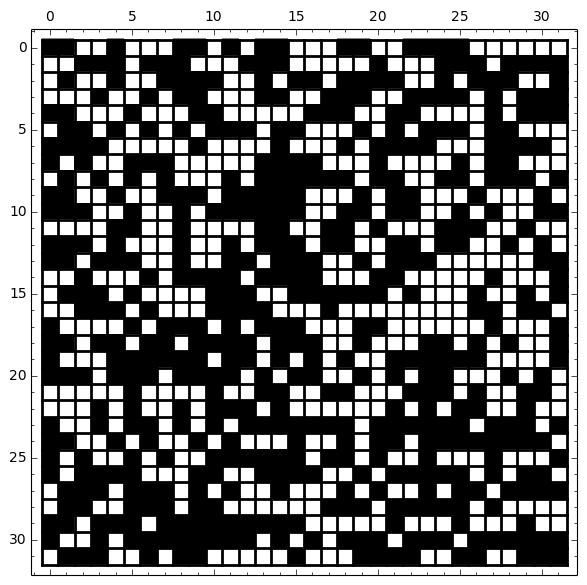
\includegraphics[scale=0.5]{figures/BC_lfsr_ex1.png}
\end{center}
\caption{Visualization of the pseudo-random bit sequence from Figure~\ref{Sage-code-bool-psr},
   generated by SageMath sample~\ref{Sage-code-bool-psr}
   (1 = black, 0 = white)}\label{fig-bool-lfsr2}
\end{figure}
% \clearpage

\subsection{Algebraic
   Attack\index{algebraic attack}\index{attack!algebraic}
   on LFSRs}\label{ss-bool-alg2}

Even simple random generators\index{random generator} such as LFSRs\index{LFSR}
produce bit sequences that are virtually indistiguishable from true random sequences
by statistical methods, and so provide no hooks for statistical methods of cryptanalysis.
This is not true for attacks with known
plaintext\index{known plaintext}\index{plaintext!known}. The resulting equations
for the key bits are accessible for algebraic
cryptanalysis\index{algebraic cryptanalysis}\index{cryptanalysis!algebraic}. If
the key stream originates from a known source trying to solve these equations
promises success. In particular this holds for LFSRs.

Consider a key bitstream $u_0, u_1, \ldots$ generated by an LFSR\index{LFSR}
by formulas~(\ref{eq-bool-lfsr1}) or (\ref{eq-bool-lfsr2}). Assume a
plaintext $a$ is XOR encrypted using this key stream\index{key stream},
resulting in the ciphertext $c$, where $c_i = a_i + u_i$ for $i = 0, 1, \ldots$
What are the prospects of an attacker who knows a chunk of the plaintext?

Well, assume she knows the first $l+1$ bits\footnote{%
   If she knows any $l+1$ bits, even non-contiguous, the idea of attack
   is the same, only the formalism is slightly more involved.
} of the plaintext. She immediately
derives the corresponding bits $u_0, \ldots, u_l$ of the key stream, in
particular the initial state of the LFSR. For the yet unknown coefficients
$s_i$ she knows a linear relation:
\[
     s_1 u_{l-1} + \cdots + s_l u_0 = u_l.
\]
Each additional known plaintext bit yields one more relation, and having
$l$ relations, from $2l$ bits of known plaintext, the easy linear
algebra\index{linear algebra}\index{algebra!linear} over the field $\F_2$
(in non-degenerate cases) finds a unique solution. In the next subsections
we'll prove, using some deeper mathematical methods:

\begin{theorem}\label{thm-bool-lfsr}
  An LFSR\index{LFSR} of length $l$ is completely predictable from the first $2l$
  bits for the cost of about $\frac{1}{3} \cdot l^3$ bit operations.
\end{theorem}

\subsubsection*{Prediction of LFSRs}

Assume we know the first $2l$ bits $u_0, \ldots, u_{2l-1}$ from an
LFSR\index{LFSR} of length $l$. For an elegant formulation of the linear algebra
methods we introduce the {\bf state vectors\index{state vector}}
\[
     u_{(i)} = (u_i, \ldots, u_{i+l-1}) \quad \text{for } i = 0, 1, \ldots
\]
The vector $u_{(i)}$ is the register content for step $i$ (in reversed order
compared with Figure~\ref{fig-bool-fsr}).
Thus the analysis focusses on the states, not directly on the output. The
recursion~(\ref{eq-bool-lfsr1}) in matrix form (for $n \geq l$) is
\[
     \begin{pmatrix} u_{n-l+1} \\ \vdots \\ u_{n-1} \\ u_{n} \end{pmatrix}
     =
     \begin{pmatrix} 0      & 1      & \ldots & 0      \\
                     \vdots & \vdots & \ddots & \vdots \\
                     0      & 0      & \ldots & 1      \\
                     s_l    & s_{l-1}    & \ldots & s_1 \end{pmatrix}
     \begin{pmatrix} u_{n-l} \\ \vdots \\ u_{n-2} \\ u_{n-1} \end{pmatrix}
\]
or more parsimoniously (the indices being substituted by $m = n-l+1$)
\[
     u_{(m)} = S \cdot u_{(m-1)} \quad \text{for } m \geq 1
\]
where $S$ is the coefficient matrix. As a further step we collect $l$
consecutive state vectors $u_{(i)}, \ldots, u_{(i+l-1)}$ in a state matrix
\[
     U_{(i)} = \begin{pmatrix} u_i      & u_{i+1}      & \ldots & u_{i+l-1}      \\
                               u_{i+1} & u_{i+2} & \ldots & u_{i+l} \\
                               \vdots  & \vdots & \ddots & \vdots     \\
                     u_{i+l-1}    & u_{i+l} & \ldots & u_{2l-2} \end{pmatrix}
\]
and set $U = U_{(0)}$, $V = U_{(1)}$. This gives the formula
\[
     V  =  S \cdot U
\]
that expresses the unknown coefficients $s_1, \ldots, s_l$ by the known
plaintext bits $u_0, \ldots, u_{2l-1}$. Most notably it allows us to write
down the solution immediately---provided that the matrix $U$ is invertible:
\[
     S  =  V \cdot U^{-1}.
\]
The matrix $S$ explicitly displays the coefficients $s_1, \ldots, s_l$.
We'll discuss the invertibility later on.

\subsubsection*{Example}

Assume we are given a ciphertext:
\begin{verbatim}
   10011100 10100100 01010110 10100110 01011101 10101110
   01100101 10000000 00111011 10000010 11011001 11010111
   00110010 11111110 01010011 10000010 10101100 00010010
   11000110 01010101 00001011 11010011 01111011 10110000
   10011111 00100100 00001111 01010011 11111101
\end{verbatim}
We suspect that the cipher is XOR with a key stream from an LFSR of
length $l = 16$. The context suggest that the text is in German and
begins with the word ``Treffpunkt'' (meeting point). To solve the
cryptogram we need 32 bits of plaintext, that is the first four letters
only, presupposed that the theory applies. This gives 32 bits of the
key stream:
\begin{verbatim}
    01010100 01110010 01100101 01100110 = T r e f
    10011100 10100100 01010110 10100110   cipher bits
    -------- -------- -------- --------
    11001000 11010110 00110011 11000000   key bits
\end{verbatim}
SageMath sample~\ref{Sage-code-bool-lfsr2} determines the coefficient matrix.
Its last row tells us that all $s_i = 0$ except $s_{16} = s_5 = s_3 = s_2 = 1$.

Now we know the LFSR and the initial state, and can reconstruct the complete
key stream---yes, it is the same as in Figure~\ref{Sage-code-bool-psr}---and
write down the plaintext (that by the way begins a bit differently from our guess).

\begin{sagecode}
\begin{verbatim}

sage: l = 16
sage: kbits =
      [1,1,0,0,1,0,0,0,1,1,0,1,0,1,1,0,0,0,1,1,0,0,1,1,1,1,0,0,0,0,0,0]
sage: ulist = []
sage: for i in range(0,l):
        state = kbits[i:(l+i)]
        ulist.append(state)
sage: U = matrix(GF(2),ulist)
sage: det(U)
1
sage: W = U.inverse()
sage: vlist = []
sage: for i in range(1,l+1):
        state = kbits[i:(l+i)]
        vlist.append(state)
sage: V = matrix(GF(2),vlist)
sage: S = V*W
sage: S
[0 1 0 0 0 0 0 0 0 0 0 0 0 0 0 0]
[0 0 1 0 0 0 0 0 0 0 0 0 0 0 0 0]
[0 0 0 1 0 0 0 0 0 0 0 0 0 0 0 0]
[0 0 0 0 1 0 0 0 0 0 0 0 0 0 0 0]
[0 0 0 0 0 1 0 0 0 0 0 0 0 0 0 0]
[0 0 0 0 0 0 1 0 0 0 0 0 0 0 0 0]
[0 0 0 0 0 0 0 1 0 0 0 0 0 0 0 0]
[0 0 0 0 0 0 0 0 1 0 0 0 0 0 0 0]
[0 0 0 0 0 0 0 0 0 1 0 0 0 0 0 0]
[0 0 0 0 0 0 0 0 0 0 1 0 0 0 0 0]
[0 0 0 0 0 0 0 0 0 0 0 1 0 0 0 0]
[0 0 0 0 0 0 0 0 0 0 0 0 1 0 0 0]
[0 0 0 0 0 0 0 0 0 0 0 0 0 1 0 0]
[0 0 0 0 0 0 0 0 0 0 0 0 0 0 1 0]
[0 0 0 0 0 0 0 0 0 0 0 0 0 0 0 1]
[1 0 0 0 0 0 0 0 0 0 0 1 0 1 1 0]
\end{verbatim}
\caption{Determining a coefficient matrix}\label{Sage-code-bool-lfsr2}
\end{sagecode}

\subsubsection*{Proof of the Theorem}

We have shown that the cofficients are uniquely determined assuming the
state matrix $U = U_{(0)}$ is invertible. As a consequence in this case
the LFSR is completely known, and all output bits are predictable. We
have yet to discuss the case where the matrix $U$ is singular.

If one of the first $l$ state vectors (= rows of the matrix $U$) is zero,
then all following state vectors are zero too, and prediction is trivial.

Thus we may assume that none of these vectors are zero, but that they are
linearly dependent. Then there is a smallest index $k \geq 1$ such that
$u_{(k)}$ is contained in the subspace spanned by $u_{(0)}, \ldots, u_{(k-1)}$,
and we find coefficients $t_1, \ldots, t_k \in \F_2$ such that
\[
     u_{(k)}  =  t_1 u_{(k-1)} + \cdots + t_k u_{(0)}.
\]
Then also $u_{(k+1)} = S\cdot u_{(k)} = 
t_1 S\cdot u_{(k-1)} + \cdots + t_k S\cdot u_{(0)} =
t_1 u_{(k)} + \cdots + t_k u_{(1)}$, and by induction we get
\[
     u_{(n)}  =  t_1 u_{(n-1)} + \cdots + t_k u_{(n-k)}
     \quad \text{for all } n \geq k.
\]
This formula predicts all the following bits.

The statement on the cost follows from Theorem~\ref{thm-bool-lin}.

\subsubsection*{Discussion}

\begin{itemize}
   \item For a singular state matrix this consideration yields a shorter
      LFSR (of length $k < l$) that generates exactly the same sequence.
      Then our method doesn't determine the coefficients of the original
      register but nevertheless correctly predicts the sequence.
   \item If the bits the attacker knows aren't just the first ones but $2l$
      contiguous ones at a later position, then the theorem yields only the
      prediction of the following bits. In the main case of an invertible
      state matrix $U$ the LFSR is completely known and may be run backwards
      to get the previous bits. For a singular state matrix we achieve
      the same effect using the shorter LFSR constructed above.
   \item The situation where $2l$ bits of the key stream are known but
      at non-contiguous positions is slightly more involved. We get
      linear relations that contain additional (unknown) intermediate bits.
      If $m$ is the number of these then we get $l+m$ linear equations for
      $l+m$ unknown bits.
   \item What if the length $l$ of the LFSR is unknown? Exhaustively trying
      all values $l = 1, 2, 3, \ldots$ is nasty but feasible. A better approach
      is provided by the Berlekamp-Massey\footnote{%
      in SageMath contained as {\tt sage.crypto.lfsr.berlekamp\_massey}, in
      CrypTool\,2 under ``cryptanalysis''/``generic''/``Berlekamp-Massey algorithm''
      } algorithm that is efficient also without knowledge of $l$. We won't
      treat it in this chapter.
\end{itemize}

\subsubsection*{Summary}

Given a random generator\index{random generator} as in Figure~\ref{fig-bool-prg}
cryptanalytic targets are:
\begin{itemize}
\item the secret parameters,
\item the initial state,
\item additional parts of the output (``prediction problem\index{prediction problem}''),
\end{itemize}
given some parts of the output. As we saw for LFSRs\index{LFSR} the prediction
problem has a solution even when the internal parameters remain unknown. Thus:
\begin{quote}
   {\em Cryptanalysis of a random generator first of all means solving the
   prediction problem. A random generator\index{random generator} is
   cryptographically secure if its prediction problem admits no efficient
   solution.}
\end{quote}

\begin{quote}
   {\em Linear feedback shift
   registers\index{linear feedback shift register}\index{feedback shift register!linear}
   are not cryptographically secure.}
\end{quote}

\subsection{Approaches to Nonlinearity\index{nonlinearity} for Feedback Shift
   Registers}\label{ss-bool-nlsr}

LFSRs are popular---in particular among electrical engineers and military---for
several reasons:
\begin{itemize}
	\item very easy implementation,
	\item extreme efficiency in hardware,
	\item good qualification as random generators for statistical applications
         and simulations,
	\item unproblematic operation in parallel even in large quantities.
\end{itemize}
But unfortunately from a cryptological view they are completely insecure if
used naively. To capitalize their positive properties while escaping their
cryptological weakness there are several approaches.

\subsubsection*{Approach 1, Nonlinear Feedback}

Nonlinear feedback\index{feedback} follows the scheme from
Figure~\ref{fig-bool-fsr} with a nonlinear Boolean
function\index{Boolean function}\index{function!Boolean} $f$. We saw a very
simple toy example in SageMath
sample~\ref{Sage-code-bool-fsr1}. There is a general proof that
in realistic use cases NLFSRs\index{NLFSR}\footnote{%
   for Non Linear Feedback Shift Register\index{feedback shift register!nonlinear}
} are cryptographically useless
if used in the direct naive way \cite{Pom2}. We won't pursue
this approach here.

\subsubsection*{Approach 2, Nonlinear Output Filter}

The nonlinear ouput filter\index{output filter} (nonlinear feedforward)
realizes the scheme from Figure~\ref{fig-bool-nlf}. The shift register
itself is linear, the Boolean function $f$, nonlinear.

The nonlinear ouput filter is a special case of a nonlinear combiner.

\begin{figure}
\begin{center}
\begin{picture}(320,150)
  \linethickness{2pt}
  \put(20,20){\line(1,0){260}}
  \put(20,20){\line(0,1){30}}
  \put(20,50){\line(1,0){260}}
  \put(280,20){\line(0,1){30}}
  \put(260,120){\circle{30}}
  \put(256,117){$f$}

  \linethickness{1pt}
  \put(60,20){\line(0,1){30}}
  \put(100,20){\line(0,1){30}}
  \put(240,20){\line(0,1){30}}
  \put(200,20){\line(0,1){30}}
  \put(110,30){\ldots}
  \put(180,30){\ldots}

  \put(40,20){\line(0,-1){20}}
  \put(80,20){\line(0,-1){20}}
  \put(220,20){\line(0,-1){20}}
  \put(260,20){\line(0,-1){20}}
  \put(260,0){\line(-1,0){260}}
  \put(0,0){\line(0,1){35}}
  \put(0,35){\vector(1,0){20}}

  \put(260,50){\vector(0,1){53}}
  \put(220,50){\vector(1,2){29}}
  \put(80,50){\line(0,1){25}}
  \put(80,75){\vector(4,1){163}}
  \put(40,50){\line(0,1){70}}
  \put(40,120){\vector(1,0){203}}

  \put(277,120){\vector(1,0){43}}
\end{picture}
\end{center}
\caption{Nonlinear ouput filter for an LFSR}\label{fig-bool-nlf}
\end{figure}

\subsubsection*{Approach 3, Nonlinear Combiner\index{combiner}}

The nonlinear combiner uses a ``battery'' of $n$ LFSRs---preferably
of different lengths---operated in parallel. The output sequences of the LFSRs
serve as input\footnote{%
   hence the occasional denotation ``nonlinear feedforward''
} of a Boolean function\index{Boolean function}\index{function!Boolean}
$f\!\!: \F_2^n \longrightarrow \F_2$, see Figure~\ref{fig-bool-nlc}.
We'll see in Section~\ref{ss-bool-bsana} how to cryptanalyze this
random generator.

\begin{figure}
\begin{center}
\begin{picture}(350,200)
  \linethickness{2pt}
  \put(20,20){\line(1,0){260}}
  \put(20,20){\line(0,1){30}}
  \put(20,50){\line(1,0){260}}
  \put(280,20){\line(0,1){30}}

  \linethickness{1pt}
  \put(60,20){\line(0,1){30}}
  \put(100,20){\line(0,1){30}}
  \put(240,20){\line(0,1){30}}
  \put(200,20){\line(0,1){30}}
  \put(110,30){\ldots}
  \put(180,30){\ldots}

  \put(40,20){\line(0,-1){20}}
  \put(80,20){\line(0,-1){20}}
  \put(220,20){\line(0,-1){20}}
  \put(260,20){\line(0,-1){20}}
  \put(260,0){\line(-1,0){260}}
  \put(0,0){\line(0,1){35}}
  \put(0,35){\vector(1,0){20}}

  \linethickness{2pt}
  \put(20,150){\line(1,0){260}}
  \put(20,150){\line(0,1){30}}
  \put(20,180){\line(1,0){260}}
  \put(280,150){\line(0,1){30}}

  \linethickness{1pt}
  \put(60,150){\line(0,1){30}}
  \put(100,150){\line(0,1){30}}
  \put(240,150){\line(0,1){30}}
  \put(200,150){\line(0,1){30}}
  \put(110,160){\ldots}
  \put(180,160){\ldots}

  \put(40,150){\line(0,-1){20}}
  \put(80,150){\line(0,-1){20}}
  \put(220,150){\line(0,-1){20}}
  \put(260,150){\line(0,-1){20}}
  \put(260,130){\line(-1,0){260}}
  \put(0,130){\line(0,1){35}}
  \put(0,165){\vector(1,0){20}}

  \put(80,100){$\vdots$}
  \put(220,100){$\vdots$}
  \put(80,70){$\vdots$}
  \put(220,70){$\vdots$}

  \put(280,165){\vector(1,0){20}}
  \put(280,35){\vector(1,0){20}}
  \put(315,100){\oval(30,160)}
  \put(330,100){\vector(1,0){20}}
  \put(313,97){$f$}
\end{picture}
\end{center}
\caption{Nonlinear combiner}\label{fig-bool-nlc}
\end{figure}

\subsubsection*{Approach 4, Output Selection/Decimation/Clocking}

There are different ways of controlling a battery of $n$ parallel LFSRs
by another LFSR:
\begin{itemize}
   \item {\bf Output selection}\index{output selection} takes the current
      output bit of exactly one of the LFSRs from the ``battery'', depending
      on the state of the auxiliary register, and outputs it as the next
	 pseudo-random bit. More generally we could choose ``$r$ from $n$''.
   \item For {\bf decimation}\index{decimation} one usually takes $n = 1$,
      and outputs the current bit of the one battery register only if the
	 auxiliary register is in a certain state, for example its own current
      output is $1$. Of course this kind of decimation
	 applies to arbitrary bit sequences in an analogous way.
   \item For {\bf clocking}\index{clocking} we look at the state of the
      auxiliary register and depending on it decide which of the battery
	 registers to step in the current cycle (and by how many positions),
      leaving the other registers in their current states\footnote{%
	   This reminds of the control logic of rotor machines\index{rotor machine}
        in classical cryptography.
        }.
\end{itemize}
These methods turn out to be special cases of nonlinear combiners if
properly rewritten. Thus approach 3 represents the most important method of
making the best of LFSRs\index{LFSR}.

The encryption standard \href{https://en.wikipedia.org/wiki/A5/1}{A5/1}\index{A5}
for mobile communications uses three LFSRs of lengths 19, 22 und 23, each
with maximum possible period, and slightly differently clocked. It linearly
(by simple binary addition) combines the three output streams. The---even
weaker---algorithm A5/2 controls the clocking by an auxiliary register.
Both variants can be broken on a standard PC in real-time.

The Bluetooth encryption standard $\mathrm{E}_0$\index{E0} uses four LFSRs
and combines them in a nonlinear way. This method is somewhat stronger than
A5, but also too weak for real security \cite{Schm}.

\subsubsection*{Example: The Geffe generator}

The Geffe generator\index{Geffe generator} provides a simple example of
output selection. Its description is in Figure~\ref{fig-bool-gef}.
The output is $x$, if $z = 0$, and $y$, if $z = 1$. Expressed by a formula:
\begin{eqnarray*}
   u & = & \begin{cases}
              x, & \text{if } z = 0, \\
              y, & \text{if } z = 1
           \end{cases} \\
      & = & (1 - z) x + zy = x + zx + zy.
\end{eqnarray*}
This formula shows how to interpret the Geffe generator as a nonlinear
combiner with a Boolean function $f\!\!: \F_2^3 \longrightarrow \F_2$ of degree 2.
For later use we implement $f$ in SageMath sample~\ref{Sage-code-bool-gef}.

\begin{figure}
\begin{center}
\setlength{\unitlength}{1pt}
\begin{picture}(350,200)
  \linethickness{2pt}
  \put(20,20){\line(1,0){260}}
  \put(20,20){\line(0,1){30}}
  \put(20,50){\line(1,0){260}}
  \put(280,20){\line(0,1){30}}

  \linethickness{1pt}
  \put(60,20){\line(0,1){30}}
  \put(100,20){\line(0,1){30}}
  \put(240,20){\line(0,1){30}}
  \put(200,20){\line(0,1){30}}
  \put(110,30){\ldots}
  \put(180,30){\ldots}

  \put(40,20){\line(0,-1){20}}
  \put(80,20){\line(0,-1){20}}
  \put(220,20){\line(0,-1){20}}
  \put(260,20){\line(0,-1){20}}
  \put(260,0){\line(-1,0){260}}
  \put(0,0){\line(0,1){35}}
  \put(0,35){\vector(1,0){20}}

  \linethickness{2pt}
  \put(20,80){\line(1,0){260}}
  \put(20,80){\line(0,1){30}}
  \put(20,110){\line(1,0){260}}
  \put(280,80){\line(0,1){30}}

  \linethickness{1pt}
  \put(60,80){\line(0,1){30}}
  \put(100,80){\line(0,1){30}}
  \put(240,80){\line(0,1){30}}
  \put(200,80){\line(0,1){30}}
  \put(110,90){\ldots}
  \put(180,90){\ldots}

  \put(40,80){\line(0,-1){20}}
  \put(80,80){\line(0,-1){20}}
  \put(220,80){\line(0,-1){20}}
  \put(260,80){\line(0,-1){20}}
  \put(260,60){\line(-1,0){260}}
  \put(0,60){\line(0,1){35}}
  \put(0,95){\vector(1,0){20}}

  \linethickness{2pt}
  \put(50,160){\line(1,0){260}}
  \put(50,160){\line(0,1){30}}
  \put(50,190){\line(1,0){260}}
  \put(310,160){\line(0,1){30}}

  \linethickness{1pt}
  \put(90,160){\line(0,1){30}}
  \put(130,160){\line(0,1){30}}
  \put(270,160){\line(0,1){30}}
  \put(230,160){\line(0,1){30}}
  \put(140,170){\ldots}
  \put(210,170){\ldots}

  \put(70,160){\line(0,-1){20}}
  \put(110,160){\line(0,-1){20}}
  \put(250,160){\line(0,-1){20}}
  \put(290,160){\line(0,-1){20}}
  \put(290,140){\line(-1,0){260}}
  \put(30,140){\line(0,1){35}}
  \put(30,175){\vector(1,0){20}}

  \put(310,175){\line(1,0){20}}
  \put(330,175){\line(0,-1){40}}
  \put(333,152){$z$}
  \put(330,135){\line(-1,0){15}}
  \put(315,135){\vector(0,-1){25}}

  \put(280,95){\vector(1,0){20}}
  \put(288,97){$x$}
  \put(280,35){\vector(1,0){20}}
  \put(288,38){$y$}
  \put(315,65){\oval(30,90)}
  \put(330,65){\line(-1,-1){30}}
  \put(330,65){\vector(1,0){20}}
\end{picture}
\end{center}
\caption{Geffe generator}\label{fig-bool-gef}
\end{figure}

\begin{sagecode}
\begin{verbatim}

sage: geff = BoolF(str2bbl("00011100"),method="ANF")
sage: geff.printTT()
Value at 000 is 0
Value at 001 is 0
Value at 010 is 0
Value at 011 is 1
Value at 100 is 1
Value at 101 is 0
Value at 110 is 1
Value at 111 is 1
\end{verbatim}
\caption{The Geffe function}\label{Sage-code-bool-gef}
\end{sagecode}

\subsection{Implementation of a Nonlinear Combiner}\label{ss-bool-ncsr}

A nonlinear combiner\index{combiner} uses several LFSRs, operated in parallel.
This suggests an implementation of LFSRs as objects of a class {\tt LFSR}\footnote{%
   see also CrypTool\,2, ``protocols''/``LFSR'' or ``NLFSR''
}.
\newpage

\begin{description}
   \item[Class {\tt LSFR}:] ~
      \begin{description}
         \item[Attributes:] ~
            \begin{itemize}
               \item {\tt length}: the length of the register
               \item {\tt taplist} (constant): the list of coefficients (or taps)
                  that define the bits for feedback
               \item {\tt state} (variable): the state of the register
            \end{itemize}
         \item[Methods:] ~
            \begin{itemize}
               \item {\tt setLength}: define the length (used only implicitly
                  for initialization)
               \item {\tt setTaps}: define the list of taps (used only implicitly
                  for initialization)
               \item {\tt setState}: set the state of the register
               \item {\tt getLength}: output the length
               \item {\tt nextBits}: generate a given number of output bits,
                  and set the next state
            \end{itemize}
      \end{description}
\end{description}
For observing the register a method (generically called {\tt \_\_str\_\_}
in Python) is convenient that outputs the attributes in human-readable form.

The complete implementation is in SageMath sample~\ref{Sage-code-bool-lfsr3}
in Section~\ref{ss-bool-lfsrclass}.

\subsubsection*{Example: Geffe Generator\index{Geffe generator}}

First we choose\footnote{%
  using the lists of primitive polynomials from \cite{HAC}
} three LFSRs of lengths 15, 16, 17,
whose periods are $2^{15} - 1 = 32767$, $2^{16} - 1 = 65535$, and
$2^{17} - 1 = 131071$. These are pairwise coprime, see SageMath
sample~\ref{Sage-code-bool-per}. Combining their outputs (in each step)
as bitblocks of length $3$ yields a sequence with a period that has an
impressive length of $281459944554495$, about $300 \times 10^{12}$
(300 billions\footnote{%
  European billions. For Americans this are 300 trillions.
}).
SageMath sample~\ref{Sage-code-bool-regs} defines the three LFSRs. The recursive
formula for the third one, the control register {\tt reg17}, is
$u_n = u_{n-3} + u_{n-17}$, since exactly the taps 3 and 17 are ``active''.
We let each of the LFSRs generate a sequence of length 100, see SageMath
sample~\ref{Sage-code-bool-seqs}. The Geffe function combines them in
SageMath sample~\ref{Sage-code-bool-gef-seq}.

\begin{sagecode}
\begin{verbatim}

sage: n15 = 2**15 - 1; n15
32767
sage: n15.factor()
7 * 31 * 151
sage: n16 = 2**16 - 1; n16
65535
sage: n16.factor()
3 * 5 * 17 * 257
sage: n17 = 2**17 - 1; n17
131071
sage: n17.factor()
131071
sage: period = n15 * n16 * n17; period
281459944554495
\end{verbatim}
\caption{Calculating a period}\label{Sage-code-bool-per}
\end{sagecode}

\begin{sagecode}
\begin{verbatim}

sage: reg15 = LFSR([1,0,0,0,0,0,0,0,0,0,0,0,0,0,1])
sage: reg15.setState([0,1,1,0,1,0,1,1,0,0,0,1,0,0,1])
sage: print(reg15)
Length: 15 | Taps: 100000000000001 | State: 011010110001001
sage: reg16 = LFSR([0,1,1,0,1,0,0,0,0,0,0,0,0,0,0,1])
sage: reg16.setState([0,1,1,0,1,0,1,1,0,0,0,1,0,0,1,1])
sage: print(reg16)
Length: 16 | Taps: 0110100000000001 | State: 0110101100010011
sage: reg17 = LFSR([0,0,1,0,0,0,0,0,0,0,0,0,0,0,0,0,1])
sage: reg17.setState([0,1,1,0,1,0,1,1,0,0,0,1,0,0,1,1,1])
sage: print(reg17)
Length: 17 | Taps: 00100000000000001 | State: 01101011000100111
\end{verbatim}
\caption{Three LFSRs}\label{Sage-code-bool-regs}
\end{sagecode}

\begin{sagecode}
\begin{verbatim}

sage: nofBits = 100
sage: outlist15 = reg15.nextBits(nofBits)
sage: print(outlist15)
[1, 0, 0, 1, 0, 0, 0, 1, 1, 0, 1, 0, 1, 1, 0, 1, 1, 1, 0, 0,
 0, 0, 1, 0, 0, 1, 1, 0, 1, 1, 0, 1, 0, 0, 0, 0, 0, 1, 1, 1,
 0, 1, 1, 0, 1, 1, 0, 0, 0, 0, 0, 0, 1, 0, 1, 1, 0, 1, 1, 0,
 1, 1, 1, 1, 1, 1, 1, 0, 0, 1, 0, 0, 1, 0, 0, 1, 0, 1, 0, 1,
 0, 1, 1, 1, 0, 0, 0, 1, 1, 1, 0, 0, 1, 1, 0, 0, 1, 0, 1, 1]
sage: outlist16 = reg16.nextBits(nofBits)
sage: print(outlist16)
[1, 1, 0, 0, 1, 0, 0, 0, 1, 1, 0, 1, 0, 1, 1, 0, 0, 0, 1, 1,
 0, 0, 1, 1, 1, 1, 0, 0, 0, 0, 0, 0, 0, 0, 1, 1, 1, 0, 1, 1,
 1, 0, 0, 0, 1, 1, 1, 0, 0, 0, 0, 0, 1, 0, 0, 0, 1, 1, 1, 0,
 1, 1, 1, 1, 0, 1, 0, 0, 1, 0, 0, 1, 1, 1, 1, 0, 0, 1, 0, 1,
 1, 0, 1, 1, 1, 1, 0, 0, 1, 0, 1, 1, 1, 0, 0, 1, 0, 0, 0, 1]
sage: outlist17 = reg17.nextBits(nofBits)
sage: print(outlist17)
[1, 1, 1, 0, 0, 1, 0, 0, 0, 1, 1, 0, 1, 0, 1, 1, 0, 0, 0, 1,
 0, 0, 0, 0, 0, 0, 1, 1, 0, 0, 1, 1, 1, 1, 1, 1, 0, 1, 1, 0,
 1, 1, 0, 0, 0, 0, 0, 1, 1, 1, 0, 0, 0, 0, 1, 1, 0, 0, 0, 0,
 0, 0, 0, 0, 1, 1, 1, 1, 1, 1, 1, 0, 0, 1, 0, 0, 1, 0, 0, 1,
 0, 1, 0, 1, 0, 1, 0, 1, 1, 0, 0, 1, 0, 1, 1, 0, 0, 1, 1, 0]
\end{verbatim}
\caption{Three LFSR sequences}\label{Sage-code-bool-seqs}
\end{sagecode}
\clearpage

\begin{sagecode}
\begin{verbatim}

sage: outlist = []
sage: for i in range(0,nofBits):
....:     x = [outlist15[i],outlist16[i],outlist17[i]]
....:     outlist.append(geff.valueAt(x))
....: 
sage: print(outlist)
[1, 1, 0, 1, 0, 0, 0, 1, 1, 1, 0, 0, 0, 1, 1, 0, 1, 1, 0, 1,
 0, 0, 1, 0, 0, 1, 0, 0, 1, 1, 0, 0, 0, 0, 1, 1, 0, 0, 1, 1,
 1, 0, 1, 0, 1, 1, 0, 0, 0, 0, 0, 0, 1, 0, 0, 0, 0, 1, 1, 0,
 1, 1, 1, 1, 0, 1, 0, 0, 1, 0, 0, 0, 1, 1, 0, 1, 0, 1, 0, 1,
 0, 0, 1, 1, 0, 1, 0, 0, 1, 1, 0, 1, 1, 0, 0, 0, 1, 0, 0, 1]
\end{verbatim}
\caption{The combined sequence}\label{Sage-code-bool-gef-seq}
\end{sagecode}

\subsection{Correlation Attacks\index{correlation attack}---the
   Achilles Heels of Combiners}\label{ss-bool-bsana}

Let $f\!\!: \F_2^n \longrightarrow \F_2$ be the combining function of a
nonlinear combiner\index{combiner}. The number
\[
   K_f := \#\{ x = (x_1, \ldots, x_n) \in \F_2^n \:|\: f(x) = x_1 \}
\]
counts the coincidences of the value of the function with its first argument.
If it is $> 2^{n-1}$, then the probability of a coincidence,
\[
   p = \frac{1}{2^n} \cdot K_f > \frac{1}{2},
\]
is above average, and the combined output sequence ``correlates'' with the
output of the first LFSR more then expected by random. If $p < \frac{1}{2}$,
then the correlation deviates from the expected value in the other direction.

The cryptanalyst can exploit this effect in an attack with known
plaintext\index{known plaintext}\index{plaintext!known}. We suppose that
she knows the ``hardware'', that is the taps of the registers, and also
the combining function $f$. She seeks the initial states of all the LFSRs.
We assume she knows the bits $k_0, \ldots, k_{r-1}$ of the key stream\footnote{%
  for simplicity of exposition the first ones. The argument works in the
  same way for any $r$ known key bits.
}. For each of the $2^{l_1}$ initial states of the first LFSR she generates
the sequence $u_0, \ldots, u_{r-1}$, and counts the coincidences. The expected
values are
\[
   \frac{1}{r}\cdot \#\{i \:|\: u_i = k_i\} \approx
   \begin{cases}
      p & \text{for the correct initial state of LFSR 1,} \\
      \frac{1}{2} & \text{otherwise.}
   \end{cases}
\]
If $r$ is large enough, she can determine the true initial state of LFSR 1
(with high probability) for a cost of $\sim 2^{l_1}$. She continues with
the other registers, and finally identifies the complete key with a cost
of $\sim 2^{l_1} + \cdots + 2^{l_n}$. Note that the cost is exponential,
but significantly lower than the cost $\sim 2^{l_1} \cdots 2^{l_n}$ of the
naive exhaustion of the key space.

In the language of linear
cryptanalysis\index{linear cryptanalysis}\index{cryptanalysis!linear}
from \ref{ss-bool-lka} she made use of the linear
relation\index{linear relation}\index{relation!linear}
\[
     f(x_1, \ldots, x_n) \stackrel{p}{\approx} x_1
\]
for $f$. Clearly she could use any linear relation as well to reduce the
complexity of key search\footnote{%
  A more in-depth analysis of the situation leads to the notion of
  correlation immunity\index{correlation immunity} that is related with
  the linear potential\index{linear potential}\index{potential!linear}.
}.

\subsubsection*{Correlations from the Geffe generator}

From the truth table~\ref{tab-bool-gef-wt} we get the correlations produced by
the Geffe generator\index{Geffe generator}. Thus the probabilities of
coincidences are
\[
   p = \begin{cases}
          \frac{3}{4} & \text{for register 1 ($x$),} \\
          \frac{3}{4} & \text{for register 2 ($y$),} \\
          \frac{1}{2} & \text{for register 3 ($z =$ control bit).}
       \end{cases}
\]
A correlation attack easily detects the initial states of registers
1 and 2---the battery registers---given only a short piece of an output
sequence. Afterwards exhaustion finds the initial state of register 3,
the control register.

\begin{table}[h]
\begin{center}
  \begin{tabular}{|c|cccc|cccc|}\hline
      $x$    & $0$ & $0$ & $0$ & $0$ & $1$ & $1$ & $1$ & $1$ \\
      $y$    & $0$ & $0$ & $1$ & $1$ & $0$ & $0$ & $1$ & $1$ \\
      $z$    & $0$ & $1$ & $0$ & $1$ & $0$ & $1$ & $0$ & $1$ \\
    \hline
  $f(x,y,z)$ & $0$ & $0$ & $0$ & $1$ & $1$ & $1$ & $0$ & $1$ \\
    \hline
  \end{tabular}
\end{center}
\caption{Truth table of the Geffe function (in horizontal order)}\label{tab-bool-gef-wt}
\end{table}

We exploit this weakness of the Geffe generator in SageMath
sample~\ref{Sage-code-bool-gef-lp} that continues SageMath
sample~\ref{Sage-code-bool-gef}. Since we defined the linear
profile\index{linear profile}\index{profile!linear} for objects of the
class {\tt BoolMap} only, we first of all have to interpret the
function {\tt geff} as a Boolean map, that is a one-element list of
Boolean functions. Then the linear profile is represented by a matrix
of 2 columns and 8 rows. The first column {\tt [64, 0, 0, 0, 0, 0, 0, 0]}
shows the coincidences with the linear form 0 in the range. So it contains
no useful information, except the denominator $64$ that applies to all
entries. The second row {\tt [0, 0, 16, 16, 16, 16, 0, 0]} yields the
list of coincidence probabilities $p$ (after dividing it by $64$)
in Table~\ref{tab-bool-gef-korr}, using the formula
\[
     p = \frac{1}{2} \cdot (\pm \sqrt{\lambda} + 1).
\]

If $\lambda = 0$, then $p = 1/2$. If  $\lambda = 1/4$, then $p = 1/4$
or $3/4$. For deciding between these two values for $p$ we use
Table~\ref{tab-bool-gef-wt}.

\begin{table}[h]
\begin{center}
\begin{tabular}{|l|cccccccc|} \hline
  linear form     & $0$   &   $z$   &   $y$    &   $y+z$   &  $x$    &   $x+z$   &  $x+y$  & $x+y+z$ \\
  representation  & $000$ & $001$ & $010$ & $011$ & $100$ & $101$ & $110$ & $111$ \\ \hline
  potential       & $0$   & $0$   & $1/4$ & $1/4$ & $1/4$ & $1/4$ & $0$   & $0$ \\
  probability $p$ & $1/2$ & $1/2$ & $3/4$ & $1/4$ & $3/4$ & $3/4$ & $1/2$ & $1/2$ \\ \hline
\end{tabular}
\end{center}
\caption{Coincidence probabilities of the Geffe function}\label{tab-bool-gef-korr}
\end{table}

\begin{sagecode}
\begin{verbatim}

sage: g = BoolMap([geff])
sage: linProf = g.linProf(); linProf
[[64,0], [0,0], [0,16], [0,16], [0,16], [0,16], [0,0], [0,0]]
\end{verbatim}
\caption{Linear profile of the Geffe function}\label{Sage-code-bool-gef-lp}
\end{sagecode}

In SageMath sample~\ref{Sage-code-bool-gef-coi} we apply this finding to the
$100$ element sequence from SageMath sample~\ref{Sage-code-bool-gef-seq}.
The function {\tt coinc} from SageMath sample~\ref{Sage-code-bool-div-bbl}
(in the appendix) counts the coincidences. For the first register we
find $73$ coincidences, for the second one $76$, for the third one
only $41$. This confirms the values $75$, $75$, $50$ predicted by our theory
(taking into account statistical variability).

\begin{sagecode}
\begin{verbatim}

sage: coinc(outlist15,outlist)
73
sage: coinc(outlist16,outlist)
76
sage: coinc(outlist17,outlist)
41
\end{verbatim}
\caption{Coincidences for the Geffe generator}\label{Sage-code-bool-gef-coi}
\end{sagecode}

\subsubsection*{Cryptanalysis of the Geffe Generator\index{Geffe generator}}

These results promise an effortless analysis of our sample sequence. For an
assessment of the success probability
we consider a bitblock $b \in \F_2^r$ and first ask how large is the
probability that a random bitblock $u \in \F_2^r$ coincides with $b$ at
exactly $t$ positions. For an answer we have to look at the symmetric binomial
distribution\index{binomial distribution} (where $p = \frac{1}{2}$ is
the probability of coincidence at a single position): The probability of
exactly $t$ coincidences is
\[
     B_{r,\frac{1}{2}}(t)  =  \frac{\binom{r}{t}}{2^r}.
\]
Hence the cumulated probability of up to $T$ coincidences is
\[
     \sum_{t=0}^T B_{r,\frac{1}{2}}(t)
       =  \frac{1}{2^r} \cdot \sum_{t=0}^T \binom{r}{t}.
\]
If $r$ is not too large, then we may explicitly calculate this value
for a given bound $T$. If on the other hand $r$ is not too small, then
we approximate the value using the normal distribution\index{normal distribution}.
The mean value of the number of coincidences is $r/2$, the variance, $r/4$,
and the standard deviation, $\sqrt{r}/2$.

In any case for $r = 100$ the probability of finding at most (say) $65$
coincidences is $0.999$, the probability of surpassing this number
is 1\,\textperthousand. For the initial state of register 1 we have to
try $2^{15} = 32786$ possibilities (generously including the zero
state $0 \in \F_2^{15}$ into the count). So we expect about $33$
oversteppings with at least $66$ coincidences. One of these should
occur for the true initial state of register 1 that we expect to produce
about $75$ coincidences. Maybe it even produces the maximum number
of coincidences.

\begin{sagecode}
\begin{verbatim}

sage: clist = []
sage: histogr = [0] * (nofBits + 1)
sage: for i in range(0,2**15):
....:     start = int2bbl(i,15)
....:     reg15.setState(start)
....:     testlist = reg15.nextBits(nofBits)
....:     c = coinc(outlist,testlist)
....:     histogr[c] += 1
....:     clist.append(c)
....:     
sage: print(histogr)
[0, 0, 0, 0, 0, 0, 0, 0, 0, 0, 0, 0, 0, 0, 0, 0, 0, 0, 0, 0, 0,
 0, 0, 0, 0, 0, 0, 0, 0, 0, 0, 0, 0, 4, 12, 12, 37, 78, 116, 216,
 329, 472, 722, 1003, 1369, 1746, 1976, 2266, 2472, 2531, 2600,
 2483, 2355, 2149, 1836, 1574, 1218, 928, 726, 521, 343, 228, 164,
 102, 60, 47, 36, 13, 8, 7, 4, 2, 1, 2, 0, 0, 0, 0, 0, 0, 0, 0, 0,
 0, 0, 0, 0, 0, 0, 0, 0, 0, 0, 0, 0, 0, 0, 0, 0, 0, 0]
sage: mm = max(clist)
sage: ix = clist.index(mm)
sage: block = int2bbl(ix,15)
sage: print "Maximum =", mm, "at index", ix, ", start value", block
Maximum = 73 at index 13705 , start value\
 [0, 1, 1, 0, 1, 0, 1, 1, 0, 0, 0, 1, 0, 0, 1]
\end{verbatim}
\caption{Analysis of the Geffe generator---register 1}\label{Sage-code-bool-gef-ana1}
\end{sagecode}

SageMath sample~\ref{Sage-code-bool-gef-ana1} shows that this really
happens. However the maximum number of coincidences, $73$, occurs
twice in the histogram. The first occurrence happens at index
$13705$, corresponding to the initial state $011010110001001$,
the correct solution. The second occurrence, at index $31115$, see SageMath
sample~\ref{Sage-code-bool-gef-ana1a}, yields the false solution
$111100110001011$ that eventually leads to a contradiction.

\begin{sagecode}
\begin{verbatim}

sage: ix = clist.index(mm,13706); ix
31115
sage: print int2bbl(ix,15)
[1, 1, 1, 1, 0, 0, 1, 1, 0, 0, 0, 1, 0, 1, 1]
\end{verbatim}
\caption{Analysis of the Geffe generator---continued}\label{Sage-code-bool-gef-ana1a}
\end{sagecode}

SageMath sample~\ref{Sage-code-bool-gef-ana2} shows the analogous analysis
of register 2. Here the maximum of coincidences, $76$, is unique,
occurs at index $27411$ corresponding to the initial state $0110101100010011$,
and provides the correct solution.

\begin{sagecode}
\begin{verbatim}

sage: clist = []
sage: histogr = [0] * (nofBits + 1)
sage: for i in range(0,2**16):
....:     start = int2bbl(i,16)
....:     reg16.setState(start)
....:     testlist = reg16.nextBits(nofBits)
....:     c = coinc(outlist,testlist)
....:     histogr[c] += 1
....:     clist.append(c)
....:     
sage: print(histogr)
[0, 0, 0, 0, 0, 0, 0, 0, 0, 0, 0, 0, 0, 0, 0, 0, 0, 0, 0, 0,
 0, 0, 0, 0, 0, 0, 0, 1, 0, 2, 3, 4, 8, 17, 25, 51, 92, 171,
 309, 477, 750, 1014, 1423, 1977, 2578, 3174, 3721, 4452, 4821,
 5061, 5215, 5074, 4882, 4344, 3797, 3228, 2602, 1974, 1419,
 1054, 669, 434, 306, 174, 99, 62, 38, 19, 10, 3, 0, 1, 0, 0,
 0, 0, 1, 0, 0, 0, 0, 0, 0, 0, 0, 0, 0, 0, 0, 0, 0, 0, 0, 0,
 0, 0, 0, 0, 0, 0, 0]
sage: mm = max(clist)
sage: ix = clist.index(mm)
sage: block = int2bbl(ix,16)
sage: print "Maximum =", mm, "at index", ix, ", start value", block
Maximum = 76 at index 27411 , start value\
 [0, 1, 1, 0, 1, 0, 1, 1, 0, 0, 0, 1, 0, 0, 1, 1]
\end{verbatim}
\caption{Analysis of the Geffe generator---register 2}\label{Sage-code-bool-gef-ana2}
\end{sagecode}

To complete the analysis we must yet determine the initial state of register 3,
the control register. The obvious idea is to exhaust the $2^{17}$ different
possibilities. There is a shortcut since we already know $51$ of the first
$100$ bits of the control register: At a position where the values of registers
1 and 2 differ, the control bit is necessarily 0 if the final output coincides
with register 1, and 1 otherwise. Only at positions where registers 1 and 2
coincide the corresponding bit of register 3 is undetermined.
\begin{verbatim}
 register 1: 10010001101011011100001001101101000001110110110000
 register 2: 11001000110101100011001111000000001110111000111000
 register 3: -1-00--0-1101-110001---00-1-00-1--1101--110---0---
bitsequence: 11010001110001101101001001001100001100111010110000

        ... 00101101101111111001001001010101110001110011001011
        ... 00100011101111010010011110010110111100101110010001
        ... ----110-------1-1-11-0-100----01--01-1-001-1-00-1-
        ... 00100001101111010010001101010100110100110110001001
\end{verbatim}
In particular we already know 11 of the 17 initial bits, and are left with only
$2^6 = 64$ possibilities to try.

But even this may be further simplified, since the known and the unknown
bits obey linear relations of the type $u_n = u_{n-3} + u_{n-17}$.
The unknown bits of the initial state are $u_0$, $u_2$, $u_5$, $u_6$, $u_8$,
$u_{13}$. The solution follows the columns of Table~\ref{tab-bool-gef_ana3},
that immediately give
\[
     u_0 = 1,\: u_2 = 1,\: u_6 = 0.
\]
The remaining solutions are
\[
    u_8 = u_{22} = u_{39} = 0,\: u_5 = u_{22} + 1 = u_8 + 1 = 1,\:
    u_{13} = u_{30} + 1 = 0.
\]
Hence the initial state of the control register is {\tt 01101011000100111},
and we know this is the correct solution. We don't need to bother with the
second possible solution for register 1 since we already found a constellation
that correctly reproduces the sequence.

\begin{table}
\begin{center}
\begin{tabular}{c|c|c|c}
   $u_{17}=u_{14}+u_0$    & $0=1+u_0$              & $u_0=1$                &                   \\
   $u_{19}=u_{16}+u_2$    & $1=0+u_2$              & $u_2=1$                &                   \\
   $u_{20}=u_{17}+u_3$    & $u_{20}=0+0$           & $u_{20}=0$             &                   \\
   $u_{22}=u_{19}+u_5$    & $u_{22}=u_5+1$         & $u_5=u_{22}+1$         &                   \\
   $u_{23}=u_{20}+u_6$    & $0=u_{20}+u_6$         & $u_6=u_{20}$           & $u_6=0$           \\
   $u_{25}=u_{22}+u_8$    & $u_{25}=u_{22}+u_8$    & $u_8=u_{22}+u_{25}$    & $u_8=u_{22}$      \\
   $u_{27}=u_{24}+u_{10}$ & $u_{27}=0+1$           & $u_{27}=1$             &                   \\
   $u_{28}=u_{25}+u_{11}$ & $0=u_{25}+0$           & $u_{25}=0$             &                   \\
   $u_{30}=u_{27}+u_{13}$ & $u_{30}=u_{27}+u_{13}$ & $u_{13}=u_{27}+u_{30}$ & $u_{13}=u_{30}+1$ \\
   $u_{33}=u_{30}+u_{16}$ & $u_{33}=u_{30}+0$      & $u_{30}=u_{33}$        & $u_{30}=1$        \\
   $u_{36}=u_{33}+u_{19}$ & $0=u_{33}+1$           & $u_{33}=1$             &                   \\
   $u_{39}=u_{36}+u_{22}$ & $u_{39}=0+u_{22}$      & $u_{22}=u_{39}$        &                   \\
   $u_{42}=u_{39}+u_{25}$ & $0=u_{39}+u_{25}$      & $u_{39}=u_{25}$        & $u_{39}=0$
\end{tabular}
\end{center}
\caption{Determination of the control register's initial state}\label{tab-bool-gef_ana3}
\end{table}

\subsection{Design Criteria for Nonlinear Combiners}

From the forgoing discussion we derive design criteria for nonlinear
combiners\index{combiner}:
\begin{itemize}
	\item The battery registers should be as long as possible.
	\item The combining function $f$ should have a low linear
        potential\index{linear potential}\index{potential!linear}.
\end{itemize}
How long should the battery registers be? There are some algorithms for
``fast'' correlation attacks using the Walsh
transformation\index{Walsh transformation}, in particular against sparse
linear feedback functions (that use only a small number of taps) \cite{MeSt}. These
don't reduce the complexity class of the attack (``exponential in the
length of the shortest register'') but reduce the cost by a significant
factor. So they are able to attack registers whose feedback functions have
up to $100$ monomials with coefficients in their ANF. As a consequence
\begin{itemize}
	\item The single LFSRs should have a length of at least 200 bits,
	   and use about $100$ taps each.
\end{itemize}
To assess the number $n$ of LFSRs we bear in mind that the combining
function should be ``correlation immune'', in particular have a low linear
potential. A well-chosen Boolean function of $16$ variables should
suffice\footnote{%
  There are no known recommendations in the literature.
}.

Rueppel\footnote{%
   Rainer A. Rueppel, Swiss cryptographer
} found an elegant way out to make the correlation attack break
down: Use a ``time-dependent'' combining function, that is a family
$(f_t)_{t \in \N}$. The bit $u_t$ of the key stream is calculated by the 
function $f_t$. We won't analyze this approach here.

Observing that the correlation attack needs knowledge of the taps, the
security could be somewhat better if the taps are secret. Then the attacker
has to perform additional exhaustions that multiply the complexity by factors
such as $2^{l_1}$ for the first LFSR alone. This scenario allows choosing LFSRs
of somewhat smaller lengths. But bear in mind that for a hardware
implementation the taps are parts of the algorithm, not of the key,
that is they are public parameters in the sense of Figure ~\ref{fig-bool-prg}.

\subsubsection*{Efficiency}

LFSRs\index{LFSR} and nonlinear combiners\index{combiner} allow efficient
realizations by special hardware that produces one bit per clock cycle. This
rate can be enlarged by parallelization. From this point of view estimating
the cost of execution on a usual PC processor is somewhat inadequate.
Splitting each of the $\geq 200$ bit registers into $4$ parts of about $64$ bits
shifting a single register requires at least 4 clock cycles, summing up to
$64$ clock cycles for $16$ registers. Add some clock cycles for the combining
function. Thus one single bit would take about $100$ clock cycles. A
2-GHz processor, even with optimized implementation, would produce at most
$2 \cdot 10^9 / 100 = 20$ million bits per second.

As a summary we note:
\begin{quote}
  {\em Using LFSRs and nonlinear combining functions we can build useful
  and fast random generators\index{random generator}, especially in hardware.}
\end{quote}

Unfortunately there is no satisfying theory for the cryptologic security of
this type of random generators, even less a mathematical proof. Security is
assessed by plausible criteria that---as for bitblock ciphers---are related
to the nonlinearity\index{nonlinearity} of Boolean
functions\index{Boolean function}\index{function!Boolean}.

\subsection{Perfect (Pseudo-) Random Generators}\label{ss-bool-rndperf}

As we saw the essential cryptologic criterion for random\index{random generator}
generators is unpredictability\index{unpredictable}. In the 1980s cryptographers,
guided by an analogy with asymmetric cryptography, found a way of modelling this
property in terms of complexity theory\index{complexity theory}:
Prediction should boil down
to a known ``hard'' algorithmic problem such as factoring\index{factoring}
or discrete\index{discrete logarithm}\index{logarithm!discrete}
logarithm. This idea established a new quality standard for random generators,
much stronger than statistical tests, but eventually building on unproven
mathematical hypotheses. Thus the situation with respect to the security
of random generators is comparable to asymmetric encryption.

As an interesting twist it soon turned out that in a certain sense
unpredictability is a universal property: For an unpredictable sequence there
is {\em no efficient algorithm at all} that distinguishes it from a true random
sequence, a seemingly much stronger requirement. See Theorem~\ref{thm-bool-YaoTh}
(Yao's theorem). This universality justifies the denomination
``perfect\index{perfect}'' for the corresponding random generators.
In particular there is no efficient statistical
test\index{statistical test}\index{test!statistical} that is able to distinguish
the output of a perfect random generator from a true random sequence. Thus,
on the theoretical side, we have a very appropriate model for random
generators that are absolutely strong from a statistical viewpoint, and
invulnerable from a cryptological viewpoint. In other words:
\begin{quote}
   {\em Perfect\index{perfect}
   random generators\index{perfect random generator}\index{random generator!perfect}
   are cryptographically secure and statistically undistinguishable from true
   random sources.}
\end{quote}
\begin{quote}
   {\em Presumably perfect random generators exist, but there is no
   complete mathematical proof ot their existence.}
\end{quote}

The first concrete approaches to the construction of perfect random generators,
the best known being the BBS generator (for Blum\index{Blum, Lenore}\footnote{%
Lenore Blum, U.\,S. American mathematician and computer scientist, *December 18, 1942
}, Blum\index{Blum, Manuel}\footnote{%
Manuel Blum, U.\,S. American mathematician and computer scientist, *April 26, 1938
}, Shub\index{Shub, Michael}\footnote{%
Michael Shub, U.\,S. American mathematician, *August 17, 1943
}),
yielded algorithms that were too slow for most practical uses
(given the then current CPUs). But modified approaches soon provided random
generators that are passably fast und nevertheless (presumably)
cryptographically secure.

\subsection{The BBS Generator}\label{ss-bool-bbs}

As with the RSA\index{RSA} cipher we consider an integer module $m$ that
is a product of two large prime numbers. For the BBS generator\index{BBS generator}
we choose\footnote{%
  for technical reasons not to be discussed here
}
{\bf Blum primes}\index{Blum prime} $p$; these are primes $\equiv 3 \bmod 4$.
A product of two Blum primes is called a {\bf Blum integer}\index{Blum integer}.

The BBS generator\index{BBS generator} works in the following way:
As a first step choose two large random Blum primes $p$ and $q$, and form
their product $m = pq$. As a second step choose a random integer seed
$s$ with $1 \leq s \leq m-1$, and coprime\footnote{%
  If we catch an $s$ not coprime with $m$, we have factorized $m$ by hazard.
  This might happen, but is extremely unlikely, and can easily be captured at
  initialization time.
}$^,$\footnote{%
  If $x_i < \sqrt{m}$, then $x_i^2 \bmod m = x_i^2$, the integer square,
  so $x_{i+1}^2$ has the same parity as $x_i$. In order to avoid
  a constant segment at the beginning of the output, often the boundary area
  $s < \sqrt{m}$, as well as $s > m - \sqrt{m}$, is excluded. However if we
  really choose $s$ as a true random value, the probability for $s$ falling
  into these boundary areas is extremely low. But to be on the safe side
  we may require $\sqrt{m} \leq s \leq m - \sqrt{m}$.
} with $m$.

Now we proceed with generating a pseudo-random sequence: Take
$x_0 = s^2 \bmod m$ as initial state\footnote{%
   We want $x_0$ to be a quadratic residue.
}, and form the sequence of inner states
of the random generator: $x_i = x_{i-1}^2 \bmod m$ for $i = 1, 2, 3, \ldots$
In each step output that last significant bit
of the binary representation, that is $u_i = x_i \bmod 2$ for
$i = 0, 1, 2, \ldots$, or in other words, the parity of $x_i$.

\subsubsection*{Example}

Of course an example with small numbers is practically irrelevant, but it
illustrates the algorithm: Take $p = 7$, $q = 11$, $m = 77$, $s = 53$. Then
$s^2 = 2809$, hence $x_0 = 37$, and $u_0 = 1$ since $x_0$ is odd. The
naive SageMath sample~\ref{Sage-code-bool-BBStoy} shows the beginning of the
sequence of states:
\begin{center}
\begin{tabular}{|c|c|c|c|c|c|}
   \hline
   $i$   &  $0$ &  $1$ &  $2$ &  $3$ & $\ldots$ \\ \hline
   $x_i$ & $37$ & $60$ & $58$ & $53$ & $\ldots$ \\
   $u_i$ &  $1$ &  $0$ &  $0$ &  $1$ & $\ldots$ \\ \hline
\end{tabular}
\end{center}

\begin{sagecode}
\begin{verbatim}

sage: p = 7
sage: q = 11
sage: m = p*q; m
77
sage: s = 53
sage: x0 = (s^2) % m; x0
37
sage: x1 = (x0^2) % m; x1
60
sage: x2 = (x1^2) % m; x2
58
sage: x3 = (x2^2) % m; x3
53
\end{verbatim}
\caption{A (much too) simple example for BBS}\label{Sage-code-bool-BBStoy}
\end{sagecode}

Treating the Blum primes $p$ and $q$ as secret is essential for the security
of the BBS generator. They serve for forming $m$ only, afterwards they
may even be destroyed. In contrast with RSA\index{RSA} there is no further
use for them. Likewise all the non-output bits of the inner states $x_i$
must be secret.

The standard distribution of SageMath contains the BBS generator. It consists
of the procedures:
\begin{itemize}
   \item {\tt random\_blum\_prime()} in the module {\tt sage.crypto.util}. To
      generate a random Blum prime $p$ with a given number $k$ of bits
      (= digits of the binary representation) call it as
      {\tt p = random\_blum\_prime(2**(k-1), 2**k)}.
      The correctness of this algorithm is only empirically founded: In fact
      there is always\footnote{%
      This is a special case of Bertrand's postulate\index{Bertrand's postulate},
      proved by Chebyshev\index{Chebyshev, Pafnuty Lvovich}
      in 1850: There is a prime between $n$ and $2n$ (for all $n \geq 2$).
      }
      a prime between $2^{k-1}$ and $2^k$ but this needn't be a Blum prime. Nevertheless
      empiricism tells us that there are lots of Blum primes in this interval,
      namely about $2^k/(k \log(2))$. Thus an attack by exhausion will fail.
   \item {\tt blum\_blum\_shub()} from {\tt sage.crypto.stream}.
      To generate a sequence of $r$ pseudo-random bits first generate two random
      Blum primes $p$ and $q$ and an initial value $x_0 = s^2 \bmod pq$, and then
      call the procedure as {\tt blum\_blum\_shub(r,x\_0,p,q)}.
\end{itemize}
SageMath sample~\ref{Sage-code-bool-bbs} demonstrates the procedure. The intermediate
results $p$, $q$, and $x_0$ are shown in Tables~\ref{tab-bool-bbs-p},
\ref{tab-bool-bbs-q}, and \ref{tab-bool-bbs-x0}, the result, in
Table~\ref{tab-bool-bits1000}. By convention $s$ as well as the factors $p$ and $q$
must be kept secret. Moreover there is no reason to reveal the product $m = pq$.
However considering the progress of factorization algorithms we better should 
use Blum integers\index{Blum integer} of at least 2048 bits\footnote{%
   more on this in Section~\ref{ss-bool-perfqr}
}.
And in any case $s$ must be a true random value! We neglected this duty by
choosing $s$ as a pure power.

\begin{sagecode}
\begin{verbatim}

sage: from sage.crypto.util import random_blum_prime
sage: from sage.crypto.stream import blum_blum_shub
sage: p = random_blum_prime(2^511, 2^512)
sage: q = random_blum_prime(2^511, 2^512)
sage: x0 = 11^248 % (p*q)             # s = 11^124 % (p*q)
sage: blum_blum_shub(1000,x0,p,q)
\end{verbatim}
\caption{Generating a sequence of BBS pseudo-random bits}\label{Sage-code-bool-bbs}
\end{sagecode}

\begin{table}[hbtp]
\begin{verbatim}
    8 445 834 617 855 090 512 176 000 413 196 767 417 799 332
  626 936 992 170 472 089 385 128 414 279 550 732 184 808 226
  736 683 775 727 426 619 339 706 269 080 823 255 441 520 165
  438 397 334 657 231 839 251
\end{verbatim}
\caption{A Blum prime $p$ with 512 bits (154 decimal places)}\label{tab-bool-bbs-p}
\end{table}

\begin{table}[hbtp]
\begin{verbatim}
   12 580 605 326 957 495 732 854 671 722 855 802 182 952 894
  232 088 903 111 155 705 856 898 413 602 721 771 810 991 595
  365 229 641 230 483 180 760 744 910 366 324 916 344 823 400
  588 340 927 883 444 616 787
\end{verbatim}
\caption{A Blum prime $q$ with 512 bits (155 decimal places)}\label{tab-bool-bbs-q}
\end{table}

\begin{table}[hbtp]
\begin{verbatim}
    1 842 408 460 334 540 507 430 929 434 383 083 145 786 026
  412 146 359 363 362 017 837 922 966 741 162 861 257 645 571
  680 482 798 249 771 263 305 761 292 545 408 040 659 753 561
  970 871 645 393 254 757 072 936 076 922 069 587 163 804 708
  256 246 366 137 431 776 175 309 050 064 068 198 002 904 756
  218 898 942 856 431 647 438 473 529 312 261 281
\end{verbatim}
\caption{An initial value $x_0$} \label{tab-bool-bbs-x0}
\end{table}

\begin{table}[hbtp]
\begin{verbatim}
  1010 0110 0011 0100 0000 0111 1111 0100 1111 0111 0010 1001
  0000 0100 1111 0000 0010 1010 1011 1111 1000 0101 1110 0011 
  1110 1000 1001 1100 1000 1000 0110 0111 0011 0011 1010 0011 
  1100 1111 0011 1000 1011 0110 1011 1110 0110 1110 0111 1000 
  1101 0011 1101 0010 1000 1101 0000 1100 0100 1011 1110 0011
  0110 0010 1011 0000 1010 1001 0110 0000 0011 1010 0011 1111 
  1010 0110 0101 1000 1011 0100 0100 1111 1010 1011 0001 1100 
  0000 0011 1101 1001 0001 0000 1111 1010 1001 0111 0111 0111 
  0000 1010 0101 0111 0111 0001 0110 1001 0011 1011 0000 0011 
  1000 0000 0111 0110 0110 1010 0110 0011 0111 1100 0010 0110 
  0011 1001 1010 1111 0001 0010 1111 0010 1100 1111 0110 0100 
  0001 1000 0101 0011 0000 0101 1111 1100 0101 0000 0100 0100 
  0100 0101 0010 1110 1010 1011 1011 0110 0101 1011 1111 1110 
  1100 1001 1011 0110 1001 0111 0111 1110 0101 0111 0011 0100 
  1101 1110 0011 1111 1101 0100 1111 1011 1010 0010 0111 1111 
  1010 1000 1100 1001 1010 1001 1010 0111 0100 0100 1010 0110 
  0011 0010 1110 0111 0101 0111 1101 0000 0110 0000 1110 1100
  0101 1010 0111 1000 0101 1111 0010 1101 0110 0100 0010 1101 
  0000 1101 0111 1011 0010 1010 1000 0110 0100 0111 1100 0000 
  1101 0000 1011 1111 0101 1011 0011 1110 0010 1110 1101 0001
  1110 1111 1000 0111 1010 0000 1100 0101 0110 0001
\end{verbatim}
\caption{1000 BBS pseudo-random bits} \label{tab-bool-bits1000}
\end{table}

\subsection{Perfectness and the Factorization Conjecture}\label{ss-bool-perfqr}

Informally we define a {\bf pseudo-random generator}\index{pseudo-random generator}
(shortly: a random generator\index{random generator}) as an efficient algorithm
that takes a ``short'' bitstring $s \in \F_2^n$ and converts it into a ``long''
bitstring\index{bitstring} $s \in \F_2^r$.

The terminology of complexity theory\index{complexity theory} allows us to give
a mathematically exact\footnote{%
   but not completey satisfying from a practical point of view
} definition by considering parameter-dependent families
of Boolean maps\index{Boolean map}
\mbox{$G_n\!: \F_2^n \longrightarrow \F_2^{r(n)}$}, and analyzing their
behaviour when the parameter $n$ grows to infinity. Such an
algorithm---represented by the family $(G_n)$ of Boolean maps---can be efficient
only if the ``expanding function'' $r\!: \N \longrightarrow \N$ grows at most
polynomially with the parameter $n$, otherwise even writing down the
output sequence in an efficient way is impossible. Then we measure the cost
somehow in a meaningful way, for example count the number of needed bit
operations that likewise must be at most polynomial with respect to the
asymptotic behaviour.

On the attacker's side we consider algorithms that predict further bits, or
aim at detecting some other weaknesses of our random generator. We analyze
the costs of these algorithms also as functions of $n$. In case the cost
grows faster than any polynomial, say exponentially, we rate the
attack as inefficient.

Pursuing this approach would require a lot of additional formalisms including
a model of probabilistic algorithms that are essential tools for the
cryptanalyst. This would take us to far apart for the moment being.
However we bear in mind that there is a mathematically correct theory
formalizing the intuitive idea of efficiency. Relying on this knowledge
we don't hesitate to reasoning the naive way, and draft the following
definition that in the given form is mathematically incorrect but might be
made correct.

\begin{definition}\label{def-bool-prg-pred}\index{predictor}
  Consider a pseudo-random generator.
  A {\bf next bit predictor} is an algorithm that takes a piece
  $u_0, \ldots, u_{r-1}$ from the beginning of the pseudo-random sequence
  and calculates the next bit $u_r$, without using the internal parameters
  of the pseudo-random generator.

  The pseudo-random generator {\bf passes the prediction test\index{prediction test}}
  if there is no efficient next bit predictor.
\end{definition}
For example LFSRs\index{LFSR} don't pass the prediction test: We constructed
an efficient next bit predictor in Theorem~\ref{thm-bool-lfsr}.

\begin{definition}\label{def-bool-prg-perf}\index{perfect pseudo-random generator}
  Consider a pseudo-random generator.
  A {\bf distinguisher}\index{distinguisher} is an algorithm that decides
  whether a given sequence is purely random\index{random sequence} or is
  generated by the pseudo-random generator, without using the internal parameters
  of the pseudo-random generator.

  The pseudo-random generator is {\bf perfect}\index{perfect} if there is
  no efficient distinguisher for it.
\end{definition}
In particular no efficient statistical test is able to distinguish a perfect
pseudo-random generator from a true random source. It is a bit of a surprise
that the seemingly much weaker property of passing the prediction test already
implies perfectness. In other words the prediction test is ``universal'':

\begin{theorem} {\rm (Yao's\footnote{%
     Andrew Yao (Y�o Q\=\i{}zh�), Chinese American computer scientist,
     *December 24, 1946 
  } criterion)}\label{thm-bool-YaoTh}
  A pseudo-random generator is perfect\index{perfect random generator}\index{random generator!perfect}
  if and only if it passes the
  prediction test.
\end{theorem}
Stated without proof.

Unfortunately this approach only gives qualitative results, and so it
is somewhat dissatisfying. However, as often in complexity theory, this
is the best we can achieve.

\subsubsection*{The (Conjectured) Perfectness of the BBS Generator}

The {\bf factorization hypothesis}\index{factorization hypothesis} states
that there is no efficient algorithm that decomposes large natural numbers
into their prime factors. This hypothesis is the base of the security of
RSA\index{RSA}, as well, as stated in Theorem~\ref{thm-bool-BBSperf}, of the
perfectness of the BBS generator\index{BBS generator}:

\begin{theorem} {\rm (Blum/Blum/Shub/Vazirani\footnote{%
  Umesh Vazirani, Indian-U.\,S. American computer scientist
}/Vazirani\footnote{%
  Vijay Vazirani, Indian-U.\,S. American computer scientist, $~^{\ast}$April 20, 1957
})}\label{thm-bool-BBSperf}
   \index{Blum, Lenore}\index{Blum, Manuel}\index{Shub, Michael}
   \index{Vazirani, Umesh}\index{Vazirani, Vijay}
   Assume the factorization hypothesis holds. Then the BBS generator
   is perfect\index{perfect}.
\end{theorem}

We omit the proof (that is quite involved). Sloppily expressed the
theorem says:
\begin{quote}
   {\em Whoever is able to predict a single bit of a BBS sequence given
   a partial sequence is also able to factor the module.}
\end{quote}
This statement assumes that the attacker knows the module $m$ of the
BBS generator. However the module might also be secret, that is, considered
as a part of the key. Assuming this the cryptographic security of BBS
should even be better---but no proof of this stronger statement seems to
be known, not even an informal one.

\subsection{Examples and Practical Considerations}\label{ss-bool-perfbsp}

We saw that the BBS generator is perfect under a plausible but unproven
assumption, the factorization hypothesis. However we don't know relevant
concrete details, for example what parameters might be inappropriate.
We know that certain initial states generate output sequences with short
periods. Some examples of this effect are known, but we are far from a complete
answer. However the security proof (depending on the factorization hypothesis)
doesn't require additional assumptions. Therefore we may confidently use the
BBS generator with a pragmatic attitude: randomly choosing the parameters
(primes and initial state) the probability of hitting ``bad'' values is
extremely low, much lower then finding a needle in a haystack, or even
in the universe.

Nevertheless some questions are crucial for getting good pseudo-random
sequences from the BBS generator\index{BBS generator} in an efficient way:
\begin{itemize}
  \item How large should we choose the module $m$?
  \item How many bits can we use for a fixed module and initial state
    without compromising the security?
\end{itemize}

The provable results---relative to the factorization hypothesis---are
qualitative only, not quantitative. The recommendation to choose a module
that escapes the known factorization methods also rests on heuristic
considerations only, and doesn't seem absolutely mandatory for a module
that itself is kept secret. The real quality of the pseudo-random bit
sequence, be it for statistical or for cryptographic applications, can
only be assessed by empirical criteria for the time being. We are confident
that the danger of generating a ``bad'' pseudo-random sequence is extremely
small\footnote{%
   �mile Borel (F�lix �douard Justin �mile Borel, French mathematician
   and politician, January 7, 1871 -- February 3, 1956)
   proposed an informal ranking of negligeability of extremely small
   probabilities: $\leq 10^{-6}$ from a human view; $\leq 10^{-15}$ from
   a terrestrial view; $\leq 10^{-45}$ from a cosmic view. By choosing a
   sufficiently large module $m$ for RSA\index{RSA} or BBS\index{BBS generator}
   we easily undercut Borel's bounds by far.
}, in any case negligeable, for modules that escape the presently known
factorization algorithms, say at least of a length of $2048$ bits,
and for a true random choice of the module and the initial state.

For the length of the useable output sequence we only know the qualitative
criterion ``at most polynomially many'' that is useless in a concrete
application. But even if we only use ``quadratically many'' bits we wouldn't
hesitate to take 4 millions bits from the generator with a  $\geq 2000$ bit
module. Should we need substantially more bits we would restart the generator
with new parameters after every few millions of bits.

An additional question suggests itself: Are we allowed to output more then
a single bit of the inner state in each iteration step to enhance the
practical benefit of the generator? At least 2 bits?

Vazirani\index{Vazirani, Umesh} and Vazirani\index{Vazirani, Vijay}, and
independently Alexi, Chor, Gold\-reich\index{Goldreich, Oded}\footnote{%
  Oded Goldreich, Israeli mathematician and computer scientist, $~^{\ast}$February 4, 1957
}, and Schnorr\index{Schnorr, Claus-Peter}\footnote{%
  Claus-Peter Schnorr, German mathematician and computer scientist, $~^{\ast}$August 4, 1943
} gave a partial answer to this question, unfortunately also a qualitative
one only: at least $\Oh(\log_2 \log_2 m)$ of the least significant bits are
``safe''. Depending on the constants that hide in the ``$\Oh$'' we need to
choose a sufficiently large module, and trust empirical experience.
A common recommendation is using $\lfloor \log_2 \log_2 m \rfloor$ bits per step.
Then for a module $m$ of 2048 bits, or roughly 600 decimal places, we can use
11 bits per step. Calculating $x^2 \bmod m$ for a $n$ bit number $m$ takes
$(\frac{n}{64})^2$ multiplications of 64-bit integers and subsequently the
same number of divisions of the type ``128 bits by 64 bits''. For $n = 2048$
this makes a total of $2 \cdot (2^5)^2 = 2048$ multiplicative operations
to generate 11 bits, or about 200 operations per bit.
A well-established rule of thumb says that a modern CPU executes one
multiplicative operation per clock cycle\footnote{%
  Special CPUs that use pipelines and parallelism are significantly faster.
}.
Thus on a 2-GHz CPU with 64-bit architecture we may expect roughly
$2\cdot 10^9 / 200 \approx 10$ million bits per second, provided the
algorithm is implemented in an optimized way. This consideration shows that the
BBS generator\index{BBS generator} is almost competitive with a software
implementation of a sufficiently secure nonlinear combiner\index{nonlinear combiner}
of LFSRs, and is fast enough for many purposes if executed on a present day CPU.

The cryptographic literature offers several pseudo-random generators that follow
similar principles as BBS\index{BBS generator}:
\begin{description}
  \item[The RSA generator\index{RSA generator} (Shamir\index{Shamir, Adi}).]
     Choose a random module $m$ of $n$ bits as a product of two large primes
     $p, q$, and an exponent $d$ that is coprime with $(p-1)(q-1)$, furthermore
     a random initial state $x = x_0$. The state transition is $x \mapsto x^d \bmod m$.
     Thus we calculate $x_i = x_{i-1}^d \bmod m$, and output the least significant bit,
     or the $\lfloor \log_2 \log_2 m \rfloor$ least significant bits. If the RSA
     generator is not perfect\index{perfect}, then there exists an efficient algorithm that
     breaks the RSA cipher\index{RSA}. Since calculating $d$-th powers is more
     expensive by a factor $n$ than squaring the cost is higher then for BBS:
     for a random $d$ the algorithm needs $\Oh(n^3)$ cycles per bit.
  \item[The index generator\index{index generator}
     (Blum\index{Blum, Manuel}/Micali\index{Micali, Silvio}).] As module choose a
     random large prime $p$ of $n$ bits, and find a primitive
     root\index{primitive root}\footnote{%
       A primitive root for $p$ is an integer whose powers run through all
       residue classes $\neq 0$ $\bmod\, p$, or in algebraic terms, a generating
       element of the multiplicative group $\bmod\, p$.
     } $a$ for $p$. Furthermore
     choose a random initial state $x = x_0$, coprime with $p-1$. Then calculate
     $x_i = a^{x_{i-1}} \bmod p$, and and ouput the most significant bit of $x_i$,
     or the $\lfloor \log_2 \log_2 p \rfloor$ most significant bits.
     The perfectness of the index generator relies on the hypothesis that calculating
     discrete logarithms\index{discrete logarithm}\index{logarithm!discrete}
     $\bmod p$ is hard. The cost per bit also is $\Oh(n^3)$.
  \item[The elliptic index generator (Kaliski).] It works like the index
     generator, but replacing the group of invertible elements of the field
     $\F_p$ by an elliptic curve\index{elliptic curve}\index{curve!elliptic}
     over $\F_p$ (such a curve is a finite group in a canonical way).
\end{description}

\subsection{The Micali-Schnorr Generator}\label{ss-bool-micsch}

Micali\index{Micali, Silvio}\footnote{%
       Silvio Micali, U.\,S. American computer scientist, $~^{\ast}$October 13, 1954
     } and Schnorr proposed a pseudo-random generator that is a descendent of
the RSA generator. Fix an odd number $d \geq 3$. The parameter set is the set of all
products $m$ of two primes $p$ and $q$ whose bit length differs by at most 1, and
such that $d$ is coprime with $(p-1)(q-1)$. For an $n$-bit number $m$ let
$h(n)$ be an integer $\approx \frac{2n}{d}$. Then the $d$-th power of an
$h(n)$-bit number is (approximately) a $2n$-bit number.

In the $i$-th step calculate $z_i = x_{i-1}^d \bmod m$. Take the first $h(n)$ bits
as the new state $x_i$, that is $x_i = \lfloor z_i/2^{n-h(n)} \rfloor$, and ouput
the remaining bits, that is $y_i = z_i \bmod 2^{n-h(n)}$. Thus the bits of the
result $z_i$ are partitioned into two {\em disjoint} parts: the new state $x_i$,
and the output $y_i$. Figure~\ref{fig-bool-micsch} illustrates this scheme.

\begin{figure}
\begin{center}
\setlength{\unitlength}{1pt}
\begin{picture}(350,175)
  \linethickness{2pt}
  \put(0,20){\line(1,0){260}}
  \put(0,20){\line(0,1){30}}
  \put(100,20){\line(0,1){15}}
  \put(0,35){\line(1,0){260}}
  \put(0,50){\line(1,0){260}}
  \put(260,20){\line(0,1){30}}

  \linethickness{1pt}
  \put(45,25){$x_2$}
  \put(175,25){$y_2$}
  \put(110,40){$x_1^d \bmod m$}
  \put(260,27){\vector(1,0){60}}
  \put(270,30){\sf output}
  \put(330,25){$y_2$}
  \put(0,20){\line(0,-1){20}}
  \put(95,20){\line(4,-1){80}}

  \linethickness{2pt}
  \put(0,90){\line(1,0){260}}
  \put(0,90){\line(0,1){30}}
  \put(100,90){\line(0,1){15}}
  \put(0,105){\line(1,0){260}}
  \put(0,120){\line(1,0){260}}
  \put(260,90){\line(0,1){30}}

  \linethickness{1pt}
  \put(45,95){$x_1$}
  \put(175,95){$y_1$}
  \put(110,110){$x_0^d \bmod m$}
  \put(10,122){\sf --- --- --- $n$ bits --- --- --- --- --- --- --- ---}
  \put(260,97){\vector(1,0){60}}
  \put(270,100){\sf output}
  \put(330,95){$y_1$}
  \put(0,90){\line(0,-1){40}}
  \put(95,90){\line(4,-1){160}}

  \linethickness{2pt}
  \put(0,160){\line(1,0){100}}
  \put(0,160){\line(0,1){15}}
  \put(100,160){\line(0,1){15}}
  \put(0,175){\line(1,0){100}}

  \linethickness{1pt}
  \put(45,165){$x_0$}
  \put(10,150){\sf --- $2n/d$ bits ---}
  \put(0,160){\line(0,-1){40}}
  \put(95,160){\line(4,-1){160}}
  \put(275,165){\sf $x_0$ has $2n/d$ bits.}
  \put(280,145){\sf $x_0^d$ has $2n$ bits.}
\end{picture}
\end{center}
\caption{Micali-Schnorr generator}\label{fig-bool-micsch}
\end{figure}

But why may we hope that this random generator is perfect\index{perfect}? This depends
on the hypothesis: There is no efficient test that distinguishes the
uniform distribution on $\{1, \ldots,m-1\}$ from the distribution of
$x^d \bmod m$ for uniformly distributed $x \in \{1, \ldots, 2^{h(n)}\}$.
If this hypothesis is true, then the Micali-Schnorr
generator\index{Micali-Schnorr generator} is perfect. This argument seems
tautologic, but heuristic considerations show a relation with the security
of RSA\index{RSA} and with factorization. Anyway we have to concede that this
``proof of security'' seems considerably more airy then that for BBS\index{BBS}.

How fast do the pseudo-random bits tumble out of the machine? As elementary
operations we again count the multiplication of two 64-bit numbers, and the
division of a 128-bit number by a 64-bit number with 64-bit quotient.
We multiply and divide by the classical algorithms\footnote{%
  Multiplication by fast Fourier transformation has an advantage only for much
  larger numbers.
}.
Thus the product of $s$ (64-bit) words and $t$ words costs $st$ elementary
operations. The cost of division is the same as the cost of the product
of divisor and quotient.

The concrete recommendation\footnote{%
  Today we would choose a larger $n$.
} by the inventors is:
$d= 7$, $n = 512$. The output of each step consists of 384 bits, withholding
128 bits as the new state. The binary power algorithm for a 128-bit number $x$
with exponent 7 costs several elementary operations:
\begin{itemize}
    \item $x$ has 128 bits, hence 2 words.
    \item $x^2$ has 256 bits, hence 4 words, and costs $2 \cdot 2 = 4$ elementary
          operations.
    \item $x^3$ has 384 bits, hence 6 words, and costs $2 \cdot 4 = 8$ elementary
          operations.
    \item $x^4$ has 512 bits, hence 8 words, and costs $4 \cdot 4 = 16$ elementary
          operations.
    \item $x^7$ has 896 bits, hence 14 words, and costs $6 \cdot 8 = 48$ elementary
          operations.
    \item $x^7 \bmod m$ has $\leq 512$ bits, and likewise costs $6 \cdot 8 = 48$
          elementary operations.
\end{itemize}
This makes a total of 124 elementary operations; among them only one reduction
$\bmod\,m$ (for $x^7$). Our reward consists of 384 pseudo-random  bits. Thus we
get about 3 bits per elementary operation, or, by the assumptions in
Section~\ref{ss-bool-perfbsp}, about 6 milliards\footnote{%
   European milliards = American billions
} bits per second. Compared with the BBS generator\index{BBS generator} this
amounts to a factor of about 1000.

Parallelization increases the speed virtually without limit: The
Micali-Schnorr generator\index{Micali-Schnorr generator} allows complete
parallelization. Thus distributing the work among $k$ CPUs brings a profit
by the factor $k$ since the CPUs can work indepedently of each other without
need of communication.

\subsection{Summary and Outlook}\label{ss-bool-prg-res}

Bitstream ciphers\index{bitstream cipher} need cryptographically secure
random generators\index{random generator}. These probably exist, however
their security---{\em like the security of almost all ciphers}---is mathematically not
completely proven.

But implementing a useful bitstream cipher takes more than
just a good random generator:
\begin{itemize}
   \item Message integrity\index{integrity} requires additional means
      such as a combination with a cryptographic hash function\index{hash function}. 
   \item The operational conditions must prevent the reuse of (parts of) the
      key stream\index{key stream} in a reliable way. This means that the
      key management\index{key management} requires utmost prudence.
      A possible approach\footnote{%
         This was a usual approach with the cipher machines of World War II.
      } is using a longtime general key that consists of
      certain inner parameters of the random generator, and use the
      remaining parameters including the initial state as one-time message
      key.
\end{itemize}

In contrast with bitblock ciphers where we have the standard AES\index{AES} (and
the outdated standard DES\index{DES}) for bitstream ciphers there is no
established standard. Closest to standardization is the
\href{http://www.ecrypt.eu.org/stream/}{eSTREAM\index{eSTREAM} portfolio}
developed in a European project from 2004 until 2008. It recommends
a bunch of several ciphers \cite{Schm}.

Unfortunately several ``proprietary'' ciphers, mostly bitstream ciphers
developed in back rooms by cryptologic amateurs, found their way into
security critical applications, relied on ``security by obscurity'', but could
easily be analyzed by reverse engineering, and teared to shreds by cryptologists.
Therefore we finish this chapter with an advice that in an analogous
form applies to all parts of cryptography:

\begin{quote}
   {\em Never trust a random generator\index{random generator} whose algorithm
   is kept secret, or for which no analysis results are publicly available.
   Statistical analyses are insufficient as security proofs, just as little
   as gargantuan periods\index{period}, or a gigantic choice of initial
   states.}
\end{quote}


% ++++++++++++++++++++++++++++++++++++++++++++++++++++++++++++++++++++++++++
\newpage
\section{Appendix: Boolean Maps in SageMath}\label{a-bool-sage}
\subsection{What's in SageMath?}

SageMath has several functions for bitblocks\index{bitblock} and Boolean
functions\index{Boolean function}\index{function!Boolean}. These are
scattered over different modules, use different data types, and have
some limitations. We could live with them. Nevertheless in this text
we mostly use our own independent (and free) implementation\footnote{%
   This is known as ``reinventing the wheel''. Forgive it in view of
   intended uniformity and consistency. Working through the functions in the
   SageMath samples should facilitate learning the algorithms. A further aspect:
   Our modules are written in pure Python and may be used without installing
   SageMath.
}.

\subsubsection*{Bitblocks\index{bitblock}}

The SageMath function \verb:binary(): converts integers into
bitstrings\index{bitstring}. Sample usage: \verb:123456789.binary():,
result: \verb:'111010110111100110100010101':.

The module \verb:sage.crypto.util: has the functions \verb:ascii_to_bin():,
\verb:bin_to_ascii():, and \verb:ascii_integer():. Somewhere else,
in \verb:sage.crypto.block_cipher.sdes:, we find a function
\verb:sdes.string_to_list(): that converts a bitstring into a list.

\subsubsection*{Logical Expressions}

Functions for logical expressions\index{logical expression}\index{expression!logical}
are in the modules
\verb:sage.logic.boolformula:,
\verb:sage.sat.converters:,
\verb:sage.sat.solvers:, and
\verb:sage.sat.boolean_polynomials:.
However these require a mode of thinking different from the approach in this
text that is adapted to cryptographic considerations.

\subsubsection*{Boolean Functions and Maps}

For dealing with Boolean functions\index{Boolean function}\index{function!Boolean}
we may look at the module \verb:sage.crypto.boolean_function:, and use its functions
\verb:truth_table():,
\verb:algebraic_normal_form():, and
\verb:walsh_hadamard_transform():\index{Walsh transformation}\index{Hadamard transformation},
that are implemented as methods of the class \verb:BooleanFunction:.

For dealing with Boolean maps\index{Boolean map}\index{map!Boolean}
we have the functions
\verb:cnf():,
\verb:linear_approximation_matrix():, and
\verb:difference_distribution_matrix():
as methods of the class \verb:SBox: from the module \verb:sage.crypto.mq.sbox:.

\subsection{New SageMath Functions for this Chapter}

The SageMath classes and functions defined in the following can be found in the
module \verb:bitciphers.sage:. They were developed with Python 3.4.1\footnote{%
   The only relevant difference with Python 2 is the operator {\tt //} for the
   division of integers.
} under OS X, and tested with SageMath 6.2.

Their usage requires a SageMath installation. In command line mode attach the module 
via the SageMath commands
\begin{quote}
  {\tt load\_attach\_path(path='/my/path', replace=False)}
\end{quote}
\begin{quote}
   {\tt attach('bitciphers.sage')}
\end{quote}
If you use the worksheet frontend (for a SageMath server), you better copy the
single functions each into an input cell\footnote{%
   A complete SageMath worksheet containing all samples of this text is available as
   {\tt bitciphers.sws}, or in human-readable PDF format as {\tt bitciphers\_sws.pdf}.
}.

\subsection{Conversion Routines for Bitblocks}\label{ss-bool-conv}

\begin{sagecode}
\begin{verbatim}

def int2bbl(number,dim):
  """Converts number to bitblock of length dim via base-2
  representation."""
  n = number                         # catch input
  b = []                             # initialize output
  for i in range(0,dim):
    bit = n % 2                      # next base-2 bit
    b = [bit] + b                    # prepend
    n = (n - bit)//2
  return b

def bbl2int(bbl):
  """Converts bitblock to number via base-2 representation."""
  ll = len(bbl)
  nn = 0                             # initialize output
  for i in range(0,ll):
    nn = nn + bbl[i]*(2**(ll-1-i))   # build base-2 representation
  return nn
\end{verbatim}
\caption{Conversion routines for bitblocks\index{bitblock}\index{bitstring}
   }\label{Sage-code-bool-conv-bbl}
\end{sagecode}

\begin{sagecode}
\begin{verbatim}

def str2bbl(bitstr):
  """Converts bitstring to bitblock."""
  ll = len(bitstr)
  xbl = []
  for k in range(0,ll):
    xbl.append(int(bitstr[k]))
  return xbl

def bbl2str(bbl):
  """Converts bitblock to bitstring."""
  bitstr = ""
  for i in range(0,len(bbl)):
    bitstr += str(bbl[i])
  return bitstr

def txt2bbl(text):
  """Converts ASCII-text to bitblock."""
  ll = len(text)
  xbl = []
  for k in range(0,ll):
    n = ord(text[k])
    by = int2bbl(n,8)
    xbl.extend(by)
  return xbl  

def bbl2sub(bbl):
  """Converts bitblock to subset."""
  ll = len(bbl)
  set = []
  for i in range(0,ll):
    if (bbl[i] == 1):
      set.append(i+1)
  return set
\end{verbatim}
\caption{Conversion routines for bitblocks\index{bitblock}
   (continued)}\label{Sage-code-bool-conv-bbl1}
\end{sagecode}

\begin{sagecode}
\begin{verbatim}

def coinc(x,y):
  """Counts coincidences between 2 lists."""
  ll = len(x)
  assert ll <= len(y), "coinc_Error: Second bitblock too short."
  nn = 0
  for i in range(0,ll):
    if (x[i] == y[i]):
      nn += 1
  return nn

def binScPr(x,y):
  """Scalar product of two binary vectors (lists) mod 2."""
  l = len(x)
  assert l == len(y), "binScPr_Error: Blocks have different lengths."
  res = 0
  for i in range (0,l):
    res += x[i] * y[i]
  return res %2

def xor(plain,key):
  """Binary addition of bitblocks.
  Crops key if longer than plain.
  Repeats key if shorter than plain.
  """ 
  lk = len(key)
  lp = len(plain)
  ciph = []
  i = 0
  for k in range(0,lp):
    cbit = (plain[k] + key[i]) % 2
    ciph.append(cbit)
    i += 1
    if i >= lk:
      i = i-lk
  return ciph
\end{verbatim}
\caption{Various compositions of
   bitblocks\index{bitblock}\index{vector}\index{scalar product}
   }\label{Sage-code-bool-div-bbl}
\end{sagecode}
\clearpage

\subsection{Matsui's Test}\label{ss-bool-mtst}

\begin{sagecode}
\begin{verbatim}

def Mats_tst(a, b, pc, compl = False):
  """Matsui's test for linear cryptanalysis"""
  NN = len(pc)
  results = []
  for pair in pc:
    ax = binScPr(a,pair[0])
    by = binScPr(b,pair[1])
    result = (ax + by) % 2
    results.append(result)
  t_0 = 0
  for bb in results:
    if bb == 0:
      t_0 = t_0 + 1
  if 2*t_0 > NN:
    if compl:
      return [t_0,1,True]
    else:
      return [t_0,0,True]
  elif 2*t_0 < NN:
    if compl:
      return [t_0,0,True]
    else:
      return [t_0,1,True]
  else:
    return [t_0,randint(0,1),False]
\end{verbatim}
\caption{Matsui's test\index{Matsui's test}}\label{Sage-code-bool-mtst}
\end{sagecode}
\clearpage

\subsection{Walsh Transformation}\label{ss-bool-walsh}

\begin{sagecode}
\begin{verbatim}

def wtr(xx):
  """Fast Walsh transform of a list of numbers"""
  max = 4096                  # max dim = 12
  ll = len(xx)
  assert ll <= max, "wtr_Error: Bitblock too long."
  dim = 0                     # dimension
  m = 1                       # 2**dimension
  while m < ll:
    dim = dim+1
    m = 2*m
  assert ll == m, "wtr_Error: Block length not a power of 2."
  x = copy(xx)                # initialize auxiliary bitblock
  y = copy(xx)                # initialize auxiliary bitblock
  mi = 1                      # actual power of 2
  for i in range(0,dim):      # binary recursion
    for k in range(0,ll):
      if ((k//mi) % 2 == 1):  # picks bit nr i
        y[k] = x[k-mi] - x[k]
      else:
        y[k] = x[k+mi] + x[k]
    for k in range(0,ll):
      x[k] = y[k]
    mi = 2*mi                 # equals 2**i in the next step
  return x
\end{verbatim}
\caption{Walsh transformation\index{Walsh transformation}\index{Hadamard transformation}
   of bitblocks}\label{Sage-code-bool-walsh}
\end{sagecode}
\newpage

\subsection{A Class for Boolean
  Functions\index{Boolean function}\index{function!Boolean}}\label{ss-bool-class}

\begin{sagecode}
\begin{verbatim}

class BoolF(object):
  """Boolean function
  Attribute: a list of bits describing the truth table of the function
  Attribute: the dimension of the domain"""

  __max = 4096                              # max dim = 12

  def __init__(self,blist,method="TT"):
    """Initializes a Boolean function with a truth table
    or by its algebraic normal form if method is ANF."""
    ll = len(blist)
    assert ll <= self.__max, "BoolF_Error: Bitblock too long."
    dim = 0                                 # dimension
    m = 1                                   # 2**dim
    while m < ll:
      dim = dim+1
      m = 2*m
    assert ll == m, "booltestError: Block length not a power of 2."
    self.__dim = dim
    if method=="TT":
      self.__tlist = blist
    else:
      self.__tlist=self.__convert(blist)

  def __convert(self,xx):
    """Converts a truth table to an ANF or vice versa."""
    x = copy(xx)                  # initialize auxiliary bitblock
    y = copy(xx)                  # initialize auxiliary bitblock
    mi = 1                        # actual power of 2
    for i in range(0,self.__dim): # binary recursion
      for k in range(0,2**(self.__dim)):
        if ((k//mi) % 2 == 1): # picks bit nr i
          y[k] = (x[k-mi] + x[k]) % 2 # XOR
        else:
          y[k] = x[k]
      for k in range(0,2**(self.__dim)):
        x[k] = y[k]
      mi = 2*mi                   # equals 2**i in the next step
    return x
\end{verbatim}
\caption{A class for Boolean functions\index{ANF}}\label{Sage-code-bool-boolF}
\end{sagecode}

\begin{sagecode}
\begin{verbatim}

  def getTT(self):
    """Returns truth table as bitlist."""
    return self.__tlist

  def valueAt(self,xx):
    """Evaluates Boolean function."""
    ll = len(xx)
    assert ll == self.__dim, "booltestError: Block has false length."
    index = bbl2int(xx)
    return self.__tlist[index]

  def getDim(self):
    """Returns dimension of definition domain."""
    return self.__dim

  def getANF(self):
    """Returns algebraic normal form as bitlist."""
    y = self.__convert(self.__tlist)
    return y

  def deg(self):
    """Algebraic degree of Boolean function"""
    y = self.__convert(self.__tlist)
    max = 0
    for i in range (0,len(y)):
      if y[i] != 0:
        b = int2bbl(i,self.__dim)
        wt = sum(b)
        if wt > max:
          max = wt
    return max
\end{verbatim}
\caption{Boolean functions\index{ANF}\index{degree!algebraic}
   (continued)}\label{Sage-code-bool-bool-f1}
\end{sagecode}

\begin{sagecode}
\begin{verbatim}

  def wspec(self):
    """Calculate Walsh spectrum."""
    ff = copy(self.__tlist)
    ll = len(ff)
    gg = []
    for i in range(0,ll):
      bit = ff[i]
      if (bit):
        gg.append(-1)
      else:
        gg.append(1)
    ff = wtr(gg)
    return ff

  def printTT(self):
    """Prints truth table to stdout."""
    for i in range(0,2**(self.__dim)):
      bb = int2bbl(i,self.__dim)
      print "Value at " + bbl2str(bb) + " is " + repr(self.__tlist[i])

  def printANF(self):
    """Prints algebraic normal form to stdout."""
    y = self.__convert(self.__tlist)
    for i in range(0,2**(self.__dim)):
      monom = int2bbl(i,self.__dim)
      print "Coefficient at " + bbl2str(monom) + " is " + repr(y[i])
\end{verbatim}
\caption{Boolean functions: Walsh spectrum\index{spectrum}\index{Walsh spectrum}
   and human-readable output}\label{Sage-code-bool-bool-f2}
\end{sagecode}
\clearpage

\subsection{A Class for Boolean
   Maps\index{Boolean map}\index{map!Boolean}}\label{ss-bool-map}

\begin{sagecode}
\begin{verbatim}

class BoolMap(object):
  """Boolean map
  Attribute: a list of Boolean functions
  Attribute: the dimensions of domain and range"""

  __max = 8                                # max dim = 8

  def __init__(self,flist):
    """Initializes a Boolean map with a list of Boolean functions."""
    qq = len(flist)
    assert qq <= self.__max, "BoolMap_Error: Too many components."
    ll = len(flist[0].getTT())
    dim = 0                                 # dimension
    m = 1                                   # 2**dim
    while m < ll:
      dim = dim+1
      m = 2*m
    assert ll == m, "BoolMap_Error: Block length not a power of 2."
    assert dim <= self.__max, "BoolMap_Error: Block length exceeds maximum."
    self.__dimd = dim
    self.__dimr = qq
    for i in range(1,qq):
      li = len(flist[i].getTT())
      assert li == ll,  "BoolMap_Error: Blocks of different lengths."
    self.__flist = flist

  def getFList(self):
    """Returns component list."""
    return self.__flist

  def getDim(self):
    """Returns dimension of preimage and image domain."""
    return [self.__dimd, self.__dimr]
\end{verbatim}
\caption{A class for Boolean maps}\label{Sage-code-bool-bool-map}
\end{sagecode}

\begin{sagecode}
\begin{verbatim}

  def getTT(self):
    """Returns truth table as list of bitlists."""
    nn = 2**(self.__dimd)
    qq = self.__dimr
    clist = []
    for j in range(0,qq):
      clist.append(self.__flist[j].getTT())
    transp = []
    for j in range(0,nn):
      trrow = []
      for i in range(0,qq):
        trrow.append(clist[i][j])
      transp.append(trrow)
    return transp

  def printTT(self):
    """Prints truth table to stdout."""
    nn = 2**(self.__dimd)
    qq = self.__dimr
    print("Dimensions of truth table:", nn, "by", qq)
    clist = []
    for j in range(0,qq):
      clist.append(self.__flist[j].getTT())
    transp = []
    for j in range(0,nn):
      trrow = []
      for i in range(0,qq):
        trrow.append(clist[i][j])
      transp.append(trrow)
    for j in range(0,nn):
      bb = int2bbl(j,self.__dimd)
      print("Value at", bb, "is", transp[j])

  def valueAt(self,xx):
    """Evaluates Boolean map."""
    ll = len(xx)
    assert ll == self.__dimd, "boolF_Error: Block has false length."
    index = bbl2int(xx)
    vlist = []
    for j in range(0,self.__dimr):
      vlist.append(self.__flist[j].getTT()[index])
    return vlist
\end{verbatim}
\caption{Boolean maps (continued)}\label{Sage-code-bool-bool-map1}
\end{sagecode}

\begin{sagecode}
\begin{verbatim}

  def wspec(self):
    """Calculate Walsh spectrum."""
    dd = self.getDim()
    tt = self.getTT()
    m = 2**(dd[0])
    t = 2**(dd[1])
    nullv = [0] * t
    charF = []
    for k in range(0,m):
      charF.append(copy(nullv))
    for k in range(0,m):
      index = bbl2int(tt[k])
      charF[k][index] = 1
    blist = []
    for k in range(0,m):
      blist.extend(charF[k])
    speclist = wtr(blist)
    specmat = []
    for k in range(0,m):
      specmat.append(speclist[k*t:k*t+t])
    return specmat

  def linApprTable(self):
    """Calculate the linear approximation table."""
    lpr = self.wspec()
    dd = self.getDim()
    m = 2**(dd[0])
    t = 2**(dd[1])
    for k in range(0,m):
      for i in range(0,t):
        lpr[k][i] = (lpr[k][i] + m)//2
    return lpr
\end{verbatim}
\caption{Boolean maps\index{spectrum}\index{Walsh spectrum}
   (continued)}\label{Sage-code-bool-bool-map2}
\end{sagecode}
\clearpage

\begin{sagecode}
\begin{verbatim}

  def linProf(self, extended=False):
    """Calculate linear profile. If extended is True, also
       calculate maximum potential and corresponding linear forms."""
    lpr = self.wspec()
    dd = self.getDim()
    m = 2**(dd[0])
    t = 2**(dd[1])
    for k in range(0,m):
      for i in range(0,t):
        lpr[k][i] = lpr[k][i] * lpr[k][i]
    if extended:
      flatlist = []
      for row in lpr:
        flatlist.extend(row)
      denominator = flatlist.pop(0)
      mm = max(flatlist)
      ixlist = []
      for k in range(0,m):
        for i in range(0,t):
          if lpr[k][i] == mm:
            ixlist.append([k,i])
      return [lpr, mm, denominator, ixlist]
    else:
      return lpr
\end{verbatim}
\caption{Boolean maps: linear
   profile\index{linear profile}\index{profile!linear}}\label{Sage-code-bool-bool-map3}
\end{sagecode}
\clearpage

\subsection{Lucifer and Mini-Lucifer}\label{ss-bool-lucmin}

\begin{sagecode}
\begin{verbatim}

#-------------- Define S0 ----------------------------
f1 = BoolF([1,1,0,1,1,1,1,0,0,0,0,0,1,0,0,1])
f2 = BoolF([1,1,1,0,1,1,0,0,0,1,0,0,0,1,1,0])
f3 = BoolF([0,1,1,1,1,0,1,0,1,1,1,0,0,0,0,0])
f4 = BoolF([0,1,1,0,0,1,1,0,0,0,1,1,1,0,1,0])
S0 = BoolMap([f1,f2,f3,f4])

#-------------- Define S0 inverse -------------------
fi1 = BoolF([0,1,1,1,1,1,1,0,1,1,0,0,0,0,0,0])
fi2 = BoolF([1,0,0,0,1,1,0,0,1,1,0,1,0,1,1,0])
fi3 = BoolF([1,1,0,1,0,1,0,1,1,0,1,1,0,0,0,0])
fi4 = BoolF([1,1,0,0,1,0,1,0,1,0,1,0,0,1,0,1])
S0inv = BoolMap([fi1,fi2,fi3,fi4])

#-------------- Define S1 ----------------------------
g1 = BoolF([0,0,1,1,0,1,0,0,1,1,0,1,0,1,1,0])
g2 = BoolF([1,0,1,0,0,0,0,1,1,1,0,0,1,1,0,1])
g3 = BoolF([1,1,1,0,1,1,0,0,0,0,0,1,1,1,0,0])
g4 = BoolF([1,0,0,1,1,1,0,0,0,1,1,0,0,1,0,1])
S1 = BoolMap([g1,g2,g3,g4])

#-------------- Define S1 inverse -------------------
gi1 = BoolF([0,1,0,0,0,1,1,0,1,0,1,0,1,1,0,1])
gi2 = BoolF([1,0,0,1,1,1,1,0,1,0,0,1,0,0,0,1])
gi3 = BoolF([1,1,0,0,1,1,0,0,1,1,1,0,0,0,1,0])
gi4 = BoolF([0,0,1,0,1,1,0,0,0,1,1,1,0,1,0,1])
S1inv = BoolMap([gi1,gi2,gi3,gi4])

def P(b):
  """Lucifer's bit permutation"""
  pb = [b[2],b[5],b[4],b[0],b[3],b[1],b[7],b[6]]
  return pb
\end{verbatim}
\caption{S-boxes and bit permutation of Lucifer\index{Lucifer}
   }\label{Sage-code-bool-Luc}
\end{sagecode}
\clearpage

\begin{sagecode}
\begin{verbatim}

def miniLuc(a,k,r):
  """Mini-Lucifer, encrypts 8-bit a with 16-bit key k over r rounds."""
  ll = len(a)
  assert ll == 8, "miniLuc_Error: Only blocks of length 8 allowed."
  lk = len(k)
  assert lk == 16, "miniLuc_Error: Only keys of length 16 allowed."
  k0 = k[0:8]          # split into subkeys
  k1 = k[8:16]
  aa = a               # round input
  # --- begin round
  for i in range(0,r): # round number is i+1
    if (i % 2 == 0):   # select round key
      rndkey = k0
    else:
      rndkey = k1
    b = xor(aa,rndkey)     # add round key
    bleft = b[0:4]         # begin substitution
    bright = b[4:8]
    bbleft = S0.valueAt(bleft)
    bbright = S1.valueAt(bright)
    bb = bbleft + bbright  # end substitution
    if (i+1 == r):         # omit permutation in last round
      aa = bb
    else:
      aa = P(bb)
  # --- end round
  if (r % 2 == 0):         # add subkey after last round
    finkey = k0
  else:
    finkey = k1
  c = xor(aa,finkey)
  return c
\end{verbatim}
\caption{Mini-Lucifer\index{Mini-Lucifer}}\label{Sage-code-bool-MiniLuc}
\end{sagecode}
\clearpage

\subsection{A Class for Linear Feedback Shift Registers}\label{ss-bool-lfsrclass}

\begin{sagecode}
\begin{verbatim}

class LFSR(object):
  """Linear Feedback Shift Register
  Attributes: the length of the register
              a list of bits describing the taps of the register
              the state
  """

  __max = 1024                              # max length

  def __init__(self,blist):
    """Initializes a LFSR with a list of taps
    and the all 0 state."""
    ll = len(blist)
    assert ll <= self.__max, "LFSR_Error: Bitblock too long."
    self.__length = ll
    self.__taplist = blist
    self.__state = [0] * ll

  def __str__(self):
    """Defines a printable string telling the internals of
    the register."""
    outstr = "Length: " + str(self.__length)
    outstr += " | Taps: " + bbl2str(self.__taplist)
    outstr += " | State: " + bbl2str(self.__state)
    return outstr

  def getLength(self):
    """Returns the length of the LFSR."""
    return self.__length

  def setState(self,slist):
    """Sets the state."""
    sl = len(slist)
    assert sl == self.__length, "LFSR_Error: Bitblock has wrong length."
    self.__state = slist
\end{verbatim}
\caption{A class for linear feedback shift registers\index{LFSR}
   }\label{Sage-code-bool-lfsr3}
\end{sagecode}

\begin{sagecode}
\begin{verbatim}

  def nextBits(self,n):
    """Returns the next n bits as a list and updates the state."""
    outlist = []
    a = self.__taplist
    u = self.__state
    for i in range (0,n):
      b = binScPr(a,u)
      c = u.pop()
      u.insert(0,b)
      outlist.append(c)
    self.__state = u
    return outlist
\end{verbatim}
\caption{A class for linear feedback shift
   registers\index{LFSR} (continued)}\label{Sage-code-bool-lfsr4}
\end{sagecode}

% ++++++++++++++++++++++++++++++++++++++++++++++++++++++++++++++++++++++++++
\begin{thebibliography}{999}
\bibitem{Bard}
    Gregory V. Bard,
    {\em Algebraic Cryptanalysis}.
    Springer, Dordrecht 2009.

\bibitem{Bric}
    Michael Brickenstein,
    {\em Boolean Gr�bner Bases -- Theory, Algorithms and Applications}
    (Dissertation TU Kaiserslautern 2009).
    Logos Verlag, Berlin 2010.
    See also ``\href{http://polybori.sourceforge.net/}{PolyBoRi --
    Polynomials over Boolean Rings}'', online:
    {\tt http://polybori.sourceforge.net/} (25 September 2014).

\bibitem{CGHM}
    D. Castro, M. Giusti, J. Heintz, G. Matera, L. M. Pardo,
    {\em The hardness of polynomial equation solving}.
    Found. Comput. Math. 3 (2003), 347--420.

\bibitem{CLOS}
    David Cox, John Little, Donal O'Shea,
    {\em Ideals, Varieties, and Algorithms}.
    Springer, New York 2007 (3rd edition).

\bibitem{CrHa}
    Yves Crama, Peter L. Hammer (eds.),
    {\em Boolean Models and Methods in Mathematics, Computer Science,
    and Engineering}.
    Cambridge University Press, New York 2010.

\bibitem{CuSt}
    Thomas W. Cusick, Pantelimon St\u{a}nic\u{a},
    {\em Cryptographic Boolean Functions and Applications}.
    Elsevier Academic Press, Amsterdam 2009.

\bibitem{DaRi}
    Joan Daemen, Vincent Rijmen,
    {\em The Design of Rijndael. AES -- The Advanced Encryption Standard}.
    Springer, Berlin 2002.

\bibitem{GaJo}
    Michael R. Garey, David S. Johnson,
    {\em Computers and Intractability}.
    Freeman, New York 1979.

\bibitem{GaGe}
    Joachim von zur Gathen, J�rgen Gerhard,
    {\em Modern Computer Algebra}.
    Cambridge University Press, 1999.

\bibitem{Golo}
   Solomon W. Golomb,
   {\em Shift Register Sequences}.
   Revised Edition: Aegean Park Press, Laguna Hills 1982.

\bibitem{Laza}
    Daniel Lazard,
    {\em Gr�bner bases, Gaussian elimination and resolution of systems of
    algebraic equations}.
    Springer Lecture Notes in Computer Science 162
    (EUROCAL '83), 146--156.

\bibitem{LeVe}
    Arjen K. Lenstra, Eric R. Verheul,
    {\em Selecting Cryptographic Key Sizes},
    Springer Lecture Notes in Computer Science 558
    (PKC2000), p. 446--465.
    Also see ``\href{http://www.keylength.com/en/2/}{Lenstra Cryptographic
    Key Length Equations}'', online:
    {\tt http://www.keylength.com/en/2/} (19 September 2014).

\bibitem{MeSt}
    W. Meier, O. Staffelbach,
    {\em Fast correlation attacks on certain stream ciphers},
    Journal of Cryptology 1 (1989), 159--176.

\bibitem{HAC}
    Alfred J. Menezes, Paul C. van Oorschot, Scott A. Vanstone,
    {\em Handbook of Applied Cryptography}.
    CRC Press, Boca Raton 1999, online:
    \href{http://cacr.uwaterloo.ca/hac/}{\tt http://cacr.uwaterloo.ca/hac/}
   (4 January 2015)

\bibitem{Opp}
    Rolf Oppliger,
    {\em Contemporary Cryptography}.
    Artech House, Dedham MA 2011 (2nd edition).

\bibitem{PaPe}
    Christof Paar, Jan Pelzl,
    {\em Understanding Cryptography -- A Textbook for Students and Practioners}.
    Springer, 2009.

\bibitem{Pomm}
    Klaus Pommerening,
    \href{http://www.staff.uni-mainz.de/pommeren/Cryptology/Bitblock/Fourier/Fourier.pdf}{{\em Fourier
    Analysis of Boolean Maps -- A Tutorial}},
    30 May 2000, online:
    {\tt http://www.staff.uni-mainz.de} {\tt /pommeren/Kryptologie/Bitblock/A\_Nonlin/nonlin.pdf}
    (19 September 2014).

\bibitem{Pom2}
    Klaus Pommerening,
    {\em Cryptanalysis of nonlinear shift registers},
    accepted for publication in Cryptologia.
    % http://www.tandfonline.com/doi/abs/10.1080/01611194.2015.1055385

\bibitem{Schm}
    Klaus Schmeh,
    {\em Cryptography and Public Key Infrastructure on the Internet}.
    John Wiley, New York 2003.
    In German, the 6th edition was published in 2016.

\bibitem{Sege}
    A. J. M. Segers,
    {\em Algebraic Attacks from a Gr�bner Basis Perspective}.
    Master's Thesis, Technische Universiteit Eindhoven 2004. Online:
    {\tt http://www.win.tue.nl/~henkvt/images} {\tt /ReportSegersGB2-11-04.pdf}
    (22 February 2015)

\bibitem{Sta}
    Mark Stamp,
    {\em Information Security: Principles and Practice}.
    Wiley, 2011 (2nd edition).

\bibitem{Stin}
    Douglas R. Stinson,
    {\em Cryptography -- Theory and Practice}.
    Chapman \& Hall/CRC, Boca Raton 2006 (3rd edition).
\end{thebibliography}

%BERM1 \end{document}


% ..............................................................................
% Homomorphe Chiffren
% ~~~~~~~~~~~~~~~~~~~~~~~~~~~~~~~~~~~~~~~~~~~~~~~~~~~~~~~~~~~~~~~~~~~~~~~~~~~~~~

\newpage
\hypertarget{homciph}{}
\chapter{Homomorphic Ciphers}
\label{Chapter_HomomorphicCiphers}
\index{homomorphic ciphers}\index{encryption!homomorphic}
(Martin Franz, January 2013)

% -----------------------------------------------------------------------------
\section{Introduction}

Homomorphic ciphers are public-key cryptosystems with special properties. They allow performing certain arithmetic operations on encrypted ciphertexts, without knowing the corresponding plaintexts and without having to decrypt the ciphertexts first. These special properties have led to a huge amount of applications for homomorphic ciphers, e.g. in the domain of cloud computing. A very famous and relatively new cryptosystem with homomorphic properties is the Paillier cryptosystem. But also some of the older and well established cryptosystems, such as ElGamal or RSA, have homomorphic properties.


% -----------------------------------------------------------------------------
\section{Origin of the term ``homomorphic''}

We first clarify the meaning and the origin of the term ``homomorphic''. This term in cryptography is derived from its counterpart in mathematics: in mathematics, a homomorphism is a structure-preserving map between two algebraic structures. In the common sense this means, that a homomorphism $f: X \to Y$ maps the structure of $X$ to the structure of $Y$. Using an example, this can be easily illustrated: Let $(X,+)$ and $(Y,*)$ two algebraic groups with group operations $+$ and $*$, respectively. A homomorphism $f: X \to Y$ maps any given $x \in X$ to a value $y \in Y$, in a way that it holds:
%
$$f(x_1 + x_2) = f(x_1) * f(x_2)$$
%
for any two $x_1, x_2$ in $X$. This means, that for any two values $x_1, x_2$ it does not matter whether we first compute their sum (group operation of $X$) and then apply $f$ (this is the left side of the above given equation); or, whether we first apply $f$ to the values $x_1, x_2$, and then compute their product in $Y$, thus apply the group operation of $Y$. Please note that the operations $+$ and $*$ were chosen here only as an example, they always depend on the algebraic group they belong to. Naturally, the same relation holds for homomorphisms between groups with the same group operation.

\begin{example}{:} Let $X = \mathbb{Z}$ be the set of integer values. The set $\mathbb{Z}$ together with the addition operation forms an algebraic group $G_1 = (\mathbb{Z}, +)$. Similarly, the real values $\mathbb{R}$ without the value zero together with the multiplication operation form a group $G_2 = (\mathbb{R}\backslash\{0\}, *)$. The function $f:\mathbb{Z}{\to}\mathbb{R}\backslash\{0\},z {\to}e^z$ is a homomorphism, since for all $z_1,z_2 \in \mathbb{Z}$ it holds: $f(z_1+ z_2) = e^{(z_1+ z_2 )} = f(z_1 )* f(z_2)$. On the contrary, $f:\mathbb{Z} \to \mathbb{R}\backslash\{0\}, z \to z^2$ is an example for a function which is not a homomorphism.
\end{example}

% -----------------------------------------------------------------------------
\section{Decryption function is a homomorphism}

In the remainder of this chapter we will consider public-key cryptosystems with a special property, namely that its decryption function is a homomorphism. A public-key cryptosystem with this property will be called homomorphic.

Let us for now assume, the above described homomorphism $f$ is the decryption function of a known cryptosystem. This means that we can perform certain algebraic operations in the ciphertext space, knowing which effects this will have on their plaintexts. Following the above given example:

$Y$ corresponds to the set of cipher texts, $X$ is the set of plaintexts. For two plaintexts $x_1, x_2$ with corresponding ciphertexts $y_1, y_2$ it holds:
%
$$f(y_1  * y_2) = f(y_1) + f(y_2) = x_1  + x_2$$
%
This equation can be interpreted as follows: If we multiply two ciphertexts $y_1, y_2$ with each other and subsequently decrypt their product, then we will obtain the sum of the originally encrypted values $x_1$ and $x_2$. Everybody can -- without knowledge of the plaintexts, without having to decrypt and even without knowing the private decryption key -- compute a product of the two ciphertexts and knows that upon decryption the owner of the private key will obtain the sum of the two originally encrypted plaintexts.

% -----------------------------------------------------------------------------
\section{Examples of homomorphic ciphers}

\subsection{Paillier cryptosystem}

The most famous cryptosystem with homomorphic properties is the one by Paillier \cite{hc:Paillier}. First we will see how the Paillier key generation process works. After that, we will show that the Paillier cryptosystem indeed has homomorphic properties.

\subsubsection{Key generation}

First, we generate two random prime numbers $p,q$ in a way that their product $n=pq$ forms  a valid RSA modulus. As for common RSA, the value $n$ should have a bit length of at least 1024 bits.

Using the prime values $p$ and $q$, we can compute the value $\lambda = \textit{lcm}(p-1,q-1)$. $\textit{lcm}$ here denotes the least common multiple. The RSA modulus $n$ will now be the public key, while the private key is the value $\lambda$.

\subsubsection{Encryption}

Let $m$ be the message which will be encrypted, where $m$ is taken from the plaintext space $\mathbb{Z}_n$. For each encryption, we first choose a random element $r$ from the plaintext space $\mathbb{Z}_n$. Subsequently, using the public key, we compute the ciphertext $n$ as:
%
$$c = E(m,r) = (n+1)^m  * r^n  \bmod n^2$$
%
\subsubsection{Decryption}

Given the private key $\lambda$ and a ciphertext $c \in \mathbb{Z}_{n^2}^*$, we first compute $S = c^\lambda \bmod n^2$ and subsequently $T = \phi(n)^{(-1)} \bmod n^2$, where $\phi$ denotes the Euler function.

Finally, we compute the plaintext $m = D(c) = (S-1)/n * T \bmod n$.

\subsubsection{Homomorphic property}

We will now show that the Paillier cryptosystem has the homomorphic property as described above. For this, we will use $E$ to denote the encryption and $D$ to denote the decryption function of the Paillier cryptosystem. For simplicity, we set $g:= n+1$.  For any two plaintexts $m_1,m_2$ and random values $r_1, r_2$ we obtain ciphertexts $c_1, c_2$ as
%
$$c_1 = g^{m_1} *  {r_1}^n \bmod n^2 \mbox{ and } c_2 = g^{m_2} * {r_2}^n \bmod n^2,$$
%
respectively. Now it is easy to see that for the product $c_3 = c_1 * c_2$ it holds
%
$$c_3 = (g^{m_1} * {r_1}^n \bmod n^2) * (g^{m_2} * {r_2}^n \bmod n^2) = g^{m_1+m_2} * (r_1*r_2 )^n \bmod n^2 = E(m_1 + m_2, r_1*r_2)$$
%
Thus, the product of two given ciphertexts is in fact a valid ciphertext, namely the encryption of the sum of the originally encrypted messages. Now it is straightforward to see that the decryption function is a homomorphism. Given two plaintexts $m_1, m_2$ it holds
%
$$D( E(m_1,r_1) * E(m_2,r_2)) = D( E(m_1+m_2, r_1 r_2)) = m_1  + m_2 = D(E(m_1,r_1)) + D(E(m_2,r_2))$$

\subsection{Other cryptosystems}

Also older public-key cryptosystems can have homomorphic properties. Both the ElGamal cryptosystem and RSA constitute famous examples. We will show their homomorphic properties by means of some easy examples.

\subsubsection{RSA}

Let $(e,n)$ be the public RSA key ($e$ the public encryption exponent, $n$ the RSA modulus). For any two messages $m_1, m_2$ we obtain encryptions $c_1 = {m_1}^e \bmod n$ and $c_2 = {m_2}^e \bmod n$. Now for the product of these two encryptions it holds: $c_1*c_2={m_1}^e * {m_2}^e \bmod n=(m_1*m_2)^e \bmod n$. Thus, we obtain an encryption of the product of the two messages $m_1$ and $m_2$. As it is straightforward to see, this property holds for any two plaintexts $m_1, m_2$ and similar as for Paillier, the decryption function is a homomorphism. As we have seen here, RSA is an example for a homomorphism, where both groups have the same group operation.

\subsubsection{ElGamal}

Similar to RSA we can also show the homomorphic properties of the ElGamal cryptosystem. Let $(p,g,K)$ the public key while the private key is $k$ (thus, it holds $g^k \bmod p = K$). For any two messages $m_1, m_2$ and random values $r, s$ we obtain encryptions $(R, c_1) = (K^r \bmod p, m_1*g^r \bmod p)$ and $(S,c_2) = (K^s \bmod p, m_2 * g^s \bmod p)$. As for RSA, we verify that their product $(R*S, c_1*c_2)$ is an encryption of $m_1*m_2$. Again it is straightforward to see that the decryption function is a homomorphism.

% -----------------------------------------------------------------------------
\section{Applications}
The homomorphic property of the Paillier cryptosystem can be used to add two encrypted values or to multiply any value under encryption with a known constant (note that the multiplication corresponds to the repeated application of the addition operation). This makes homomorphic ciphers to important and easy to use base primitives in cryptographic applications.

\begin{enumerate}
\item One of these applications is the so called ``Electronic Voting''. Electronic voting allows a large number of voters to submit their ballots in an encrypted form. This is important in situations, where the voters cannot come together to the same location. This happens, for example, if the voters can only communicate over the internet via email. If the voting behavior of the single parties should remain secret, then the use of homomorphic ciphers is a good solution to this problem. The main principle of electronic voting using homomorphic ciphers is as follows.

All voters encrypt their ballots, using homomorphic encryption (see at the left site of the screenshot). The screenshot depicts the next steps (1 to 3):

\begin{itemize}
\item All voters (on the left in the figure \ref{CT2-PaillierVoting}) encrypt the value 1 if they opt positive and the value 0, if opposed to the decision.
\item Using the homomorphic property, one can compute the sum of all encrypted ballots. Since this happens on encrypted values, the voting behavior of all participants remains secret.
\item At the end, the result of the election is determined and published, this happens by decrypting the sum which was computed using the homomorphic property.
\end{itemize}

\begin{figure}[ht]
\begin{center}
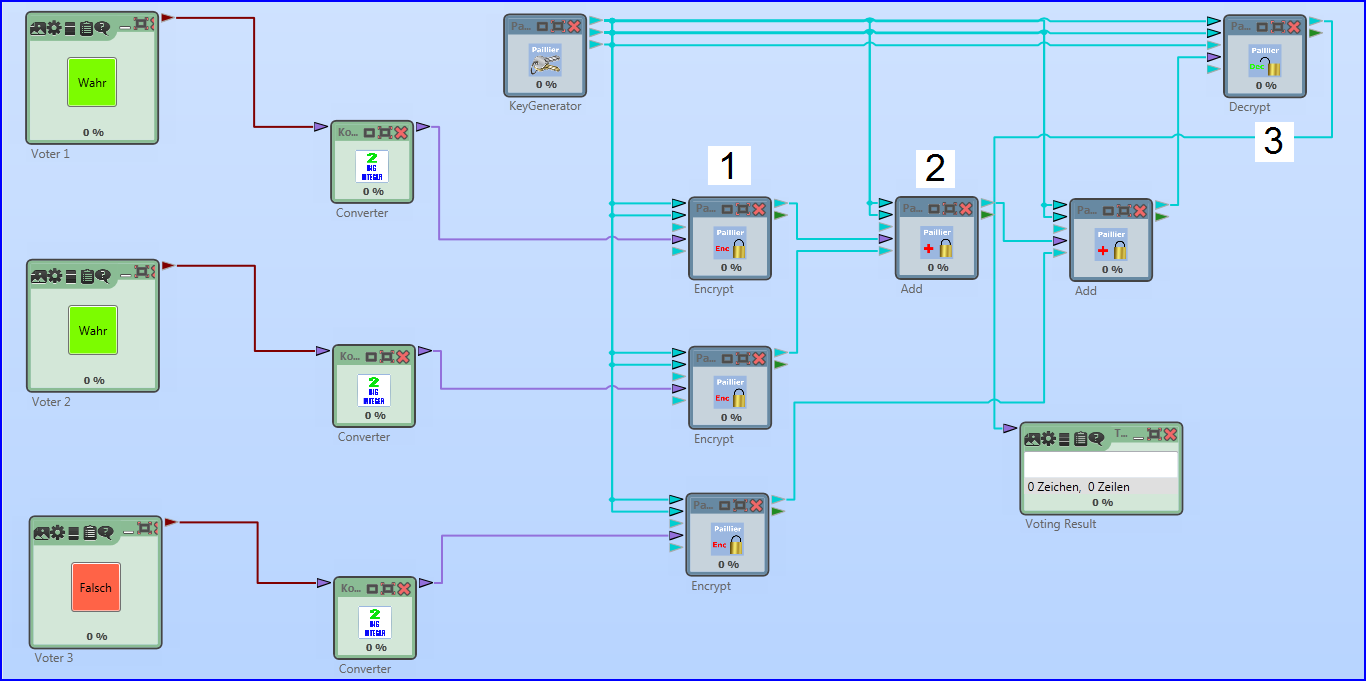
\includegraphics[scale=0.4]{figures/CT2-PaillierVoting.png}
\caption{Voting example for Paillier} 
\label{CT2-PaillierVoting}
\end{center}
\end{figure}

\item A second application of homomorphic ciphers is ``Secure Multiparty Computation''. Here, two or more parties can compute any commonly known function. Each of the parties provides one or more of the inputs for the function to be computed. The goal of the secure computations is to keep all private inputs secret, while only the result of the function is revealed. The use of homomorphic encryption helps to perform these computations on encrypted data. However, since the Paillier encryption only allows to compute additions of encrypted values (and, e.g. no multiplications can be performed), a number of additional methods and techniques have to be applied. The Wikipedia page \cite{hc:SMC} offers a great start for reading more about this topic and more advanced techniques for Secure Multiparty Computation.

\item Furthermore it is expected, that homomorphic encryption will provide great advantages in the areas of ``Cloud Computing''. Using so called ``fully-homomorphic encryption'' \cite{hc:HomEnc} it will be possible to run large applications on external servers only on encrypted data. For this, necessarily one needs to be able to perform both arithmetic operations, the addition and the multiplication, on encrypted data (in contrast to Paillier encryption, which only allows performing additions). Such a crypto system was first presented in 2009 \cite{hc:Gentry2009}.
\end{enumerate}

% -----------------------------------------------------------------------------
\section{Homomorphic ciphers in CrypTool}

\subsection{CrypTool 2}

In CrypTool 2 you will find an implementation of the Paillier cryptosystem. Among the available components, there are components for key generation (Paillier Key Generator), an example for encryption and decryption with Paillier (called Paillier Text), as well as examples which illustrate the homomorphic properties of the cryptosystem (Paillier Addition, Paillier Blinding and Paillier Voting).

\begin{figure}[ht]
\begin{center}
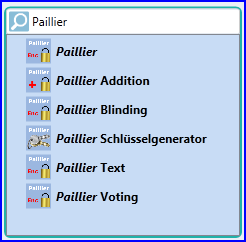
\includegraphics[scale=0.8]{figures/CT2-Paillier.png}
\caption{Paillier cryptosystem in CrypTool 2} 
\label{CT2-Paillier}
\end{center}
\end{figure}

\newpage
\subsection{JCrypTool}

In JCrypTool there is an implementation (see Figure \ref{JCT-HomEnc}), which visualizes the homomorphic properties of various cryptosystem. For RSA and Paillier it shows, that multiplications, for RSA, and additions for Paillier, respectively, can be performed on encrypted values. For the fully-homomorphic cryptosystem by Gentry it is possible to perform both multiplications, as well as additions on encrypted values.

\begin{figure}[ht]
\begin{center}
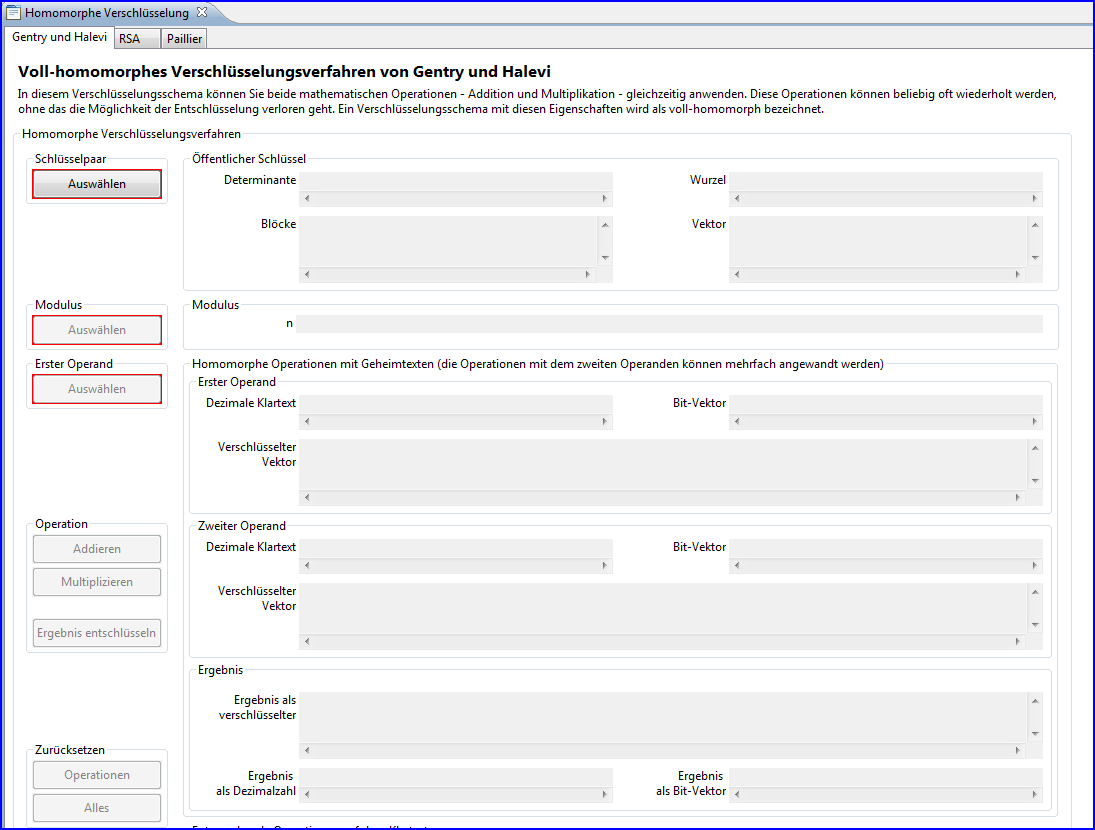
\includegraphics[scale=0.4]{figures/JCT-HomEnc.PNG}
\caption{Visualization of homomorphic properties in JCrypTool} 
\label{JCT-HomEnc}
\end{center}
\end{figure}


%------------------------------------------------------------------------------
\newpage
\begin{thebibliography}{99999}
\addcontentsline{toc}{section}{Bibliography}

\bibitem[Paillier1999]{hc:Paillier} \index{Paillier 1999}
   Pascal Paillier, \\
   {\em Public-Key Cryptosystems Based on Composite Degree Residuosity Classes},\\
	 Advances in Cryptology -- EUROCRYPT'99, 1999.

\bibitem[SMC]{hc:SMC} \index{SMC}
   Wikipedia, \\
   {\em Secure Multiparty Computation}.\\
   \url{http://en.wikipedia.org/wiki/Secure_multi-party_computation}

\bibitem[HomEnc]{hc:HomEnc}
   Wikipedia, \\
   {\em Homomorphic Encryption}\\
   \url{https://en.wikipedia.org/wiki/Homomorphic_encryption}\\
   {\em Homomorphism}\\
   \url{https://en.wikipedia.org/wiki/Homomorphism}

\bibitem[Gentry2009]{hc:Gentry2009} \index{Gentry 2009}
   Craig Gentry, \\
   {\em Fully Homomorphic Encryption Using Ideal Lattices},\\
	In the 41st ACM Symposium on Theory of Computing (STOC), 2009.

\end{thebibliography}  % German

% Local Variables:
% TeX-master: "../script-de.tex"
% End:



\bibliographyunit[\chapter]
\bibliography*{references}
\bibliographystyle*{plain}
% ..........................................................................
% --------------------------------------------------------------------------
% ++++++++++++++++++++++++++++++++++++++++++++++++++++++++++++++++++++++++++
%              Crypto 2020
% /~~~~~~~~~~~~~~~~~~~~~~~~~~~~~~~~~~~~~~~~~~~~~~~~~~~~~~~~~~~~~~~~~~~~~~~~~

\newpage
\hypertarget{Chapter_Crypto2020}{}
\chapter{Crypto 2020 --- Perspectives for Long-Term Cryptographic
         Security}\index{security!long-term}
\label{Chapter_Crypto2020}
\begin{sloppypar}
(Johannes Buchmann, Erik Dahmen, Alexander May and Ulrich Vollmer, TU Darmstadt, May~2007)\\
\end{sloppypar}

% \begin{abstract}Ever more powerful hardware and new
%   mathematical algorithms threaten to undermine
%   the security of cryptographic keys and schemes.
%   How long will the methods we use today be able
%   to keep what they promise?  And which
%   alternatives are on the horizon?
% \end{abstract}

Cryptography is a basic building block of all IT
security solutions.  Yet, for how long are the
cryptographic tools we use today going to remain
secure?  Is this time long enough to ensure the
confidentiality of medical data, to name just one
example?  Even in the short-term, the potential
for havoc is great if certain keys are broken.
Just think of the digital signatures that protect
the authenticity of automatic updates for the
Windows operating system.


\section{Widely used schemes}
\label{sec:the-weak}

In 1978, Rivest, Shamir and Adleman suggested the
RSA\index{RSA} public key encryption and signature
schemes~\cite{rivest/shamir/adleman:1978}.  RSA is
still the most widely used public key scheme.  The
security of RSA depends on the difficulty of
factoring so-called RSA moduli which are products
of two large prime numbers.  In their 1978 paper,
the inventors of RSA suggested the use of RSA
moduli with 200 decimal digits for long-term
security.  Later, the company RSA Security
published a list of RSA moduli of increasing size,
the RSA challenge numbers.  RSA Security offered
prizes totaling \$ 635,000 for the factorization
of these numbers, cf.\
\url{www.rsasecurity.com/rsalabs/}.

In 2005, that is 27 years after the invention of
RSA, Bahr, Boehm, Franke, and Kleinjung from
Bochum University managed to factor a 200 digit
RSA challenge number
(\url{www.mat.uniroma2.it/~eal/rsa640.txt}).  A
key with size originally thought to be secure for
a very long time was broken with a computation
that took them just five months.  This illustrates
the tremendous progress factoring technology has
made within the last 30 years.  This progress is
based on break-through mathematical ideas --- e.g.\
the number field sieve proposed by John
Pollard --- as well as significant developments in
computer hardware and software implementation
technology.\footnote{%
Please compare chapter \ref{SecurityRSA}
\hyperlink{SecurityRSA}{Considerations regarding the
security of the RSA algorithm}, and especially chapters
\ref{nt:NoteFactorization} and \ref{FactorizationResearch}.
}

In 2000, Lenstra and Verheul\index{Lenstra/Verheul}
developed an extrapolation formula that is supposed
to help us forecast the security\index{security!forecast}
one can achieve with RSA and other important
cryptographic schemes in the long
term (\url{www.keylength.com}).  The formula
suggests the use of 850 digit RSA moduli if one
wishes to protect data for the next 30 years.
This corresponds to a 3072 bit RSA key.

Yet, even a well thought out extrapolation formula
is no security guarantee!  At any time, a
brilliant mathematical idea can allow us to factor
large numbers easily, and destroy the security of
RSA.  In 1996, Peter Shor showed that a quantum
computer --- a new type of computer that leverages
the laws of quantum mechanics to speed up certain
types of computations --- can in principle be used
for the fast factorization of large numbers \cite{shor:1997}.
Despite intensive research in the area, it is
still too early to judge whether we are ever going
to be able to build quantum computers\index{quantum computer} of
sufficient capacity to apply Shor's algorithm to
numbers of relevant size.\footnote{%
Required qbits for attacks on RSA, DSA and ECDSA using key with a bit length n: \\
\vskip +1 pt
\begin{tabular}{|c|l|}
\hline
   RSA		&  2n + 3 \\
   DSA		&  2n + 3 \\
   ECDSA $2^n$	&  \~{}2n + 8 log n \\
   ECDSA p	&  \~{}4n \\
\hline
\end{tabular}
\vskip +6 pt
Please compare chapter 5.3 in
``SicAri -- Eine Sicherheitsplattform und deren Werkzeuge
f\"ur die ubiquit\"are Internetnutzung, KB2.1 -- Abschlussbericht,
\"Ubersicht \"uber Angriffe auf relevante kryptographische Verfahren'',
version 1.0, Mai 17, 2005,
Prof. Dr. Johannes Buchmann et al., TUD-KryptC and cv cryptovision GmbH
(\href{http://www.cdc.informatik.tu-darmstadt.de/~schepers/kb\_21\_angriffe.pdf}
 {\tt http://www.cdc.informatik.tu-darmstadt.de/\~{}schepers/kb\_21\_angriffe.pdf}) and the dissertation of Axel Schmidt at the same faculty.
}
Recent announcements of
significant progress in this area made by the
start-up company D-Wave (\url{www.dwavesys.com})
have been greeted with a lot of scepticism, even
ridicule.

The development of attacks on another frequently
used scheme called DSA (Digital Signature
Algorithm) and the Elliptic Curve Cryptography
(ECC) class of schemes moves in analogy to those
on RSA.  The security of these schemes depends on
the difficulty of computing discrete logarithms.
Even today, there is significant algorithmic
progress.  Quantum computers would render these
schemes insecure.

What's the state of affairs with the so-called
secret-key encryption schemes?  In 1977, DES was
introduced as the Data Encryption
Standard~\cite{DES-Standard:1977}.  Twenty-one
years later, the Electronic Frontier Foundation
(EFF) built the special purpose machine Deep Crack
which needed just 56 hours to break a DES key.
The problem with DES was that it used keys which
were too short.  It seems that the inventors of
DES did not foresee the speed of hardware
development.  The Advanced Encryption Standard
AES~\cite{AES-Standard:2002}, successor to DES, is
deemed secure at the moment even though there are
interesting, if still inefficient, methods to
attack AES with algebraic methods.


\section{Preparation for tomorrow}
\label{sec:preparations}

Is the security of today's cryptography measuring
up to its increasing importance?  The experience
shows: Carefully designed and implemented
cryptographic schemes have a life time of five to
twenty years.  Whoever uses RSA, ECC or AES for
short-term protection of data may feel safe.
Moreover, it is also possible to achieve long-term
authenticity, integrity and non-reputability of
data, e.g., using the multiple signature scheme
suggested by S\"onke Maseberg~\cite{maseberg-thesis:2002}.

However, current schemes cannot guarantee
long-term confidentiality.  And what is to be done in
twenty years from now?  What should we do if, quasi
over-night, unexpected mathematical progress
renders an important cryptographic scheme
insecure?  Three things are necessary to prepare
us for this event:

\begin{itemize}
\item a pool of secure alternative cryptographic schemes,
\item infrastructures that enable us to exchange
   one cryptographic scheme for another, easily
   and quickly, and
\item methods that ensure long-term confidentiality.
\end{itemize}

For many years, the cryptography group at the
Technische Universit\"at Darmstadt and its spin-off,
the company FlexSecure (\url{www.flexsecure.de}),
have worked to provide these tools.  The
trust center software FlexiTrust which is employed
by the German National Root Certification
Authority and the German Country Signing Authority
offers an infrastructure within which
cryptographic schemes can be easily exchanged.
The open source library FlexiProvider\index{FlexiProvider} implements a
multitude of cryptographic schemes.  Lately, we
have intensified our research into ``Post Quantum
Cryptography''\index{cryptography!post quantum}\index{post-quantum computing}\index{PQC} seeking
cryptographic schemes which
remain secure even in the event that powerful
quantum computers are built.

The security of public key cryptography
traditionally rests on the difficulty of the
solution of certain mathematical problems.  Today,
the following alternatives to the factorization and discrete
logarithm problems are discussed in depth:  the
decoding problem, the shortest and closest vector
problem in lattices, and the problem of solving
large systems of multivariate quadratic
equations.  It is conjectured that quantum
computers\index{quantum computer} offer little advantage if we try to
solve these problems efficiently.


\section{New mathematical problems}
\label{sec:problems}

Let us look at these alternatives a little more
closely.  The first encryption scheme based on the
decoding problem was proposed by
McEliece~\cite{mceliece:1978}\index{encryption!McEliece}.  The background:
Error-correcting codes are used to transmit or
store electronic data in such a way that they
remain undistorted even if a small number of bits
are changed in transit or on the storage media.
This property is used in, e.g., compact discs
(CDs).  The data on a CD can be reconstructed even
if the disc has been slightly scratched.

In a code-based encryption\index{encryption!code-based} scheme a message is
encrypted by adding a fixed number of errors to
(i.e. flipping a fixed numbers of bits of) the
encoded message.  Decoding requires knowledge of a
suitable decoding procedure which eliminates these
errors efficiently.  This method is the secret
key.  Code-based encryption is in general very
efficient.  At the moment, research focus on the
question which codes lead to secure encryption
schemes with keys which are as small as possible.

Encryption on the basis of lattice problems\index{encryption!lattice problems}
is very similar to that on the basis of
error-correcting codes.  Lattices are regular
structures of points in space.  For instance, the
points where the lines on squared paper cross form
a two-dimensional lattice.  For cryptographic
usage, the dimension of the lattices is chosen to
be much larger.  Encryption works as follows: The
plain-text is used to construct a lattice point
which is then slightly distorted in such a way
that it is no longer a lattice point, but close to
one.  Whoever knows a secret about the lattice is
able to find this lattice point in the vicinity of
the given point in space.  The lattice point in
turn yields the plain text.  A particularly
efficient lattice based encryption scheme is NTRU
Encrypt (\url{www.ntru.com})\index{encryption!lattice problems!NTR}.
However, because
NTRU was introduced fairly recently (in 1998), and
its specification underwent several changes due to
a variety of attacks, more cryptanalytic scrutiny
is required to achieve confidence in its security.

\section{New signatures}
\label{sec:signatures}

In 1979, Ralph Merkle proposed a remarkable
framework for new signature schemes in his PhD
thesis~\cite{merkle-thesis:1979}.
Contrary to all other signature schemes\index{signature!Merkle}, its
security does not rest on the difficulty of a
number-theoretic, algebraic or geometric problem.
The only thing it requires is something which
other signature schemes need anyway: a
cryptographically secure hash function and a
secure pseudo-random number generator.  Each new
hash function leads to a new signature algorithm.
In consequence, the Merkle scheme has the
potential to solve the problem of long-term
availability of digital signature schemes.

Merkle uses in his construction so-called One-Time
Signatures: Each new signature requires a new
signing key and a new verification key.  The idea
Merkle had was to reduce the validity of many
verification keys using a hash tree to the
validity of a unique public hash value.  When
generating keys for the Merkle scheme one has to
determine the number of signatures one can make
with it in advance.  For a long time this seemed a
significant disadvantage.  In
\cite{buchmann/coronado/dahmen/doering/klintsevich:2006},
however, a variant of Merkle's scheme was proposed
which allows to compute $2^{40}$ signatures with a
single key pair.


%\subsection{Quantum cryptography -- a loophole?}
\section{Quantum cryptography -- a way out of the impasse?}
\label{sec:quantum cryptography}\index{quantum cryptography}

From the point of view of today's state of the art
of cryptography, the problem of long-term
confidentiality remains unsolved: There is
\emph{no} practical method to protect the
confidentiality of an encrypted message over a
very long period of time.

One way out of that dilemma may be to employ
quantum cryptography: it allows for key agreement
schemes (of very long keys for one-time pads)
whose security is
guaranteed by the laws of quantum mechanics,
cf., e.g., \cite{bennett/brassard:1984b}.  At the
moment, however, quantum cryptography is still
rather inefficient, and it is unclear which
cryptographic functionalities can be implemented
on top of it.


\section{Conclusion}
\label{sec:conclusion}

What's on the balance sheet of today's cryptography?  We
have good tools to ensure short and medium term
security.  Software developers can employ these
tools in their applications with good conscience
as long as they make sure that components
can quickly be exchanged when they become
insecure.

In order to guarantee IT security for the future, too,
we need to prepare a portfolio of secure cryptographic
schemes.  This portfolio needs to contain schemes
which are suitable for the world of ubiquitous
computing with many less powerful computers.  It
also needs to contain schemes which remain secure
in the event that powerful quantum computers\index{quantum computer} are
built.  Several promising candidates have been
discussed in this article.  They need to be
studied carefully and prepared for use in everyday
scenarios.  The question how to ensure long-term
confidentiality remains an important open research
problem upon which cryptographic research should
focus.

\putbib
\addcontentsline{toc}{section}{Bibliography}   % To add it in Contents and PDF-Navigation


\bibliographyunit


% ++++++++++++++++++++++++++++++++++++++++++++++++++++++++++++++++++++++++++
\begin{appendix}
\newpage
\hypertarget{appendix-start}{}\label{s:appendix-start}
\chapter{Anhang}
    \begin{itemize}
      \item[1] \hyperlink{appendix-menu-overview-CT1}{CrypTool-1-Men�baum}
      \item[2] \hyperlink{appendix-template-overview-CT2}{CrypTool-2-Vorlagen}
      \item[3] \hyperlink{appendix-function-overview-JCT}{JCrypTool-Funktionen}
      \item[4] \hyperlink{appendix-function-overview-CTO}{CrypTool-Online-Funktionen}
      \item[5] \hyperlink{appendix-movies}{Filme und belletristische
                          Literatur mit Bezug zur Kryptographie}
      \item[6] \hyperlink{appendix-Learn-NT}
                         {Lernprogramm Elementare Zahlentheorie}
      \item[7] \hyperlink{appendix-using-sage}
                         {Kurzeinf�hrung in das Computer-Algebra-System SageMath}
      \item[8] \hyperlink{appendix-authors}{Autoren des CrypTool-Skripts}
    \end{itemize}
  % $Id%

% ++++++++++++++++++++++++++++++++++++++++++++++++++++++++++++++++++++++++++
%\pagebreak
\newpage
%\enlargethispage{1cm}
\hypertarget{appendix-menu-overview-CT1}{}
\section{CrypTool 1 Menus}
\label{s:appendix-menu-overview-CT1}

This appendix contains at the following page the complete menu tree of
CrypTool\index{CrypTool} version 1.4.31\footnote{%
  Since 2010, changes for the stable CrypTool 1 ({\bf CT1})\index{CrypTool 1}
  \index{CT1} focus mainly on bugfixes. Many new developments go into the two
  successor versions CrypTool 2 ({\bf CT2})\index{CrypTool 2}\index{CT2} and
  JCrypTool ({\bf JCT})\index{JCrypTool}\index{JCT}:\\
  - Web site CT2: \url{http://www.cryptool.org/en/ct2-documentation-en} \\
  - Web site JCT: \url{http://www.cryptool.org/en/jct-volunteer-en} \\
  These successor versions are currently (Nov. 2012) still beta versions;
  but they are close to their first release and they are stable enough
  since quite a while to be used by end-users.\\
}. 

\noindent The main menu of CT1 contains both, generic service functions in the
six main menu items
\begin{itemize}
   \item File
   \item Edit
   \item View
   \item Options
   \item Window
   \item Help,
\end{itemize}
and the actual crypto functions in the following four main menus
\begin{itemize}
   \item Encrypt / Decrypt
   \item Digital Signature / PKI
   \item Individual Procedures
   \item Analysis.
\end{itemize}

Within \verb#Individual Procedures# you find visualizations of single algorithms
and of protocols. Some procedures are implemented both for a fast performance
(mostly under the main menu \verb#Encrypt/Decrypt#) and for a step-by-step visualization.

Which of the menu items in CrypTool 1 are active (that means not greyed),
depends on the type of the currently active document window:
The brute-force analysis\index{attack!brute-force} for DES e.~g. is only
available, if the active window is opened in the hexadecimal view. 
On the other hand the menu item ``Generate Random Numbers\dots''
is always available (even if no document is opened).

%The following four types of documents exist in CrypTool:
%\begin{center}
%\begin{tabular}{rl}
%\bf Code letter & \bf Type of document \\
%T & Text file view\\
%H & Hexadecimal view\\
%P & Diagram/plot view (histogram, autocorrelation)\\
%O & OpenGL graphics view\\
%\end{tabular}
%\end{center}


%--------------------------------------------------------------------
\clearpage
\begin{figure}[hb]
\begin{center}
\vspace{-30pt}
\rotatebox{90}{%
\begin{minipage}{1.57\textwidth}
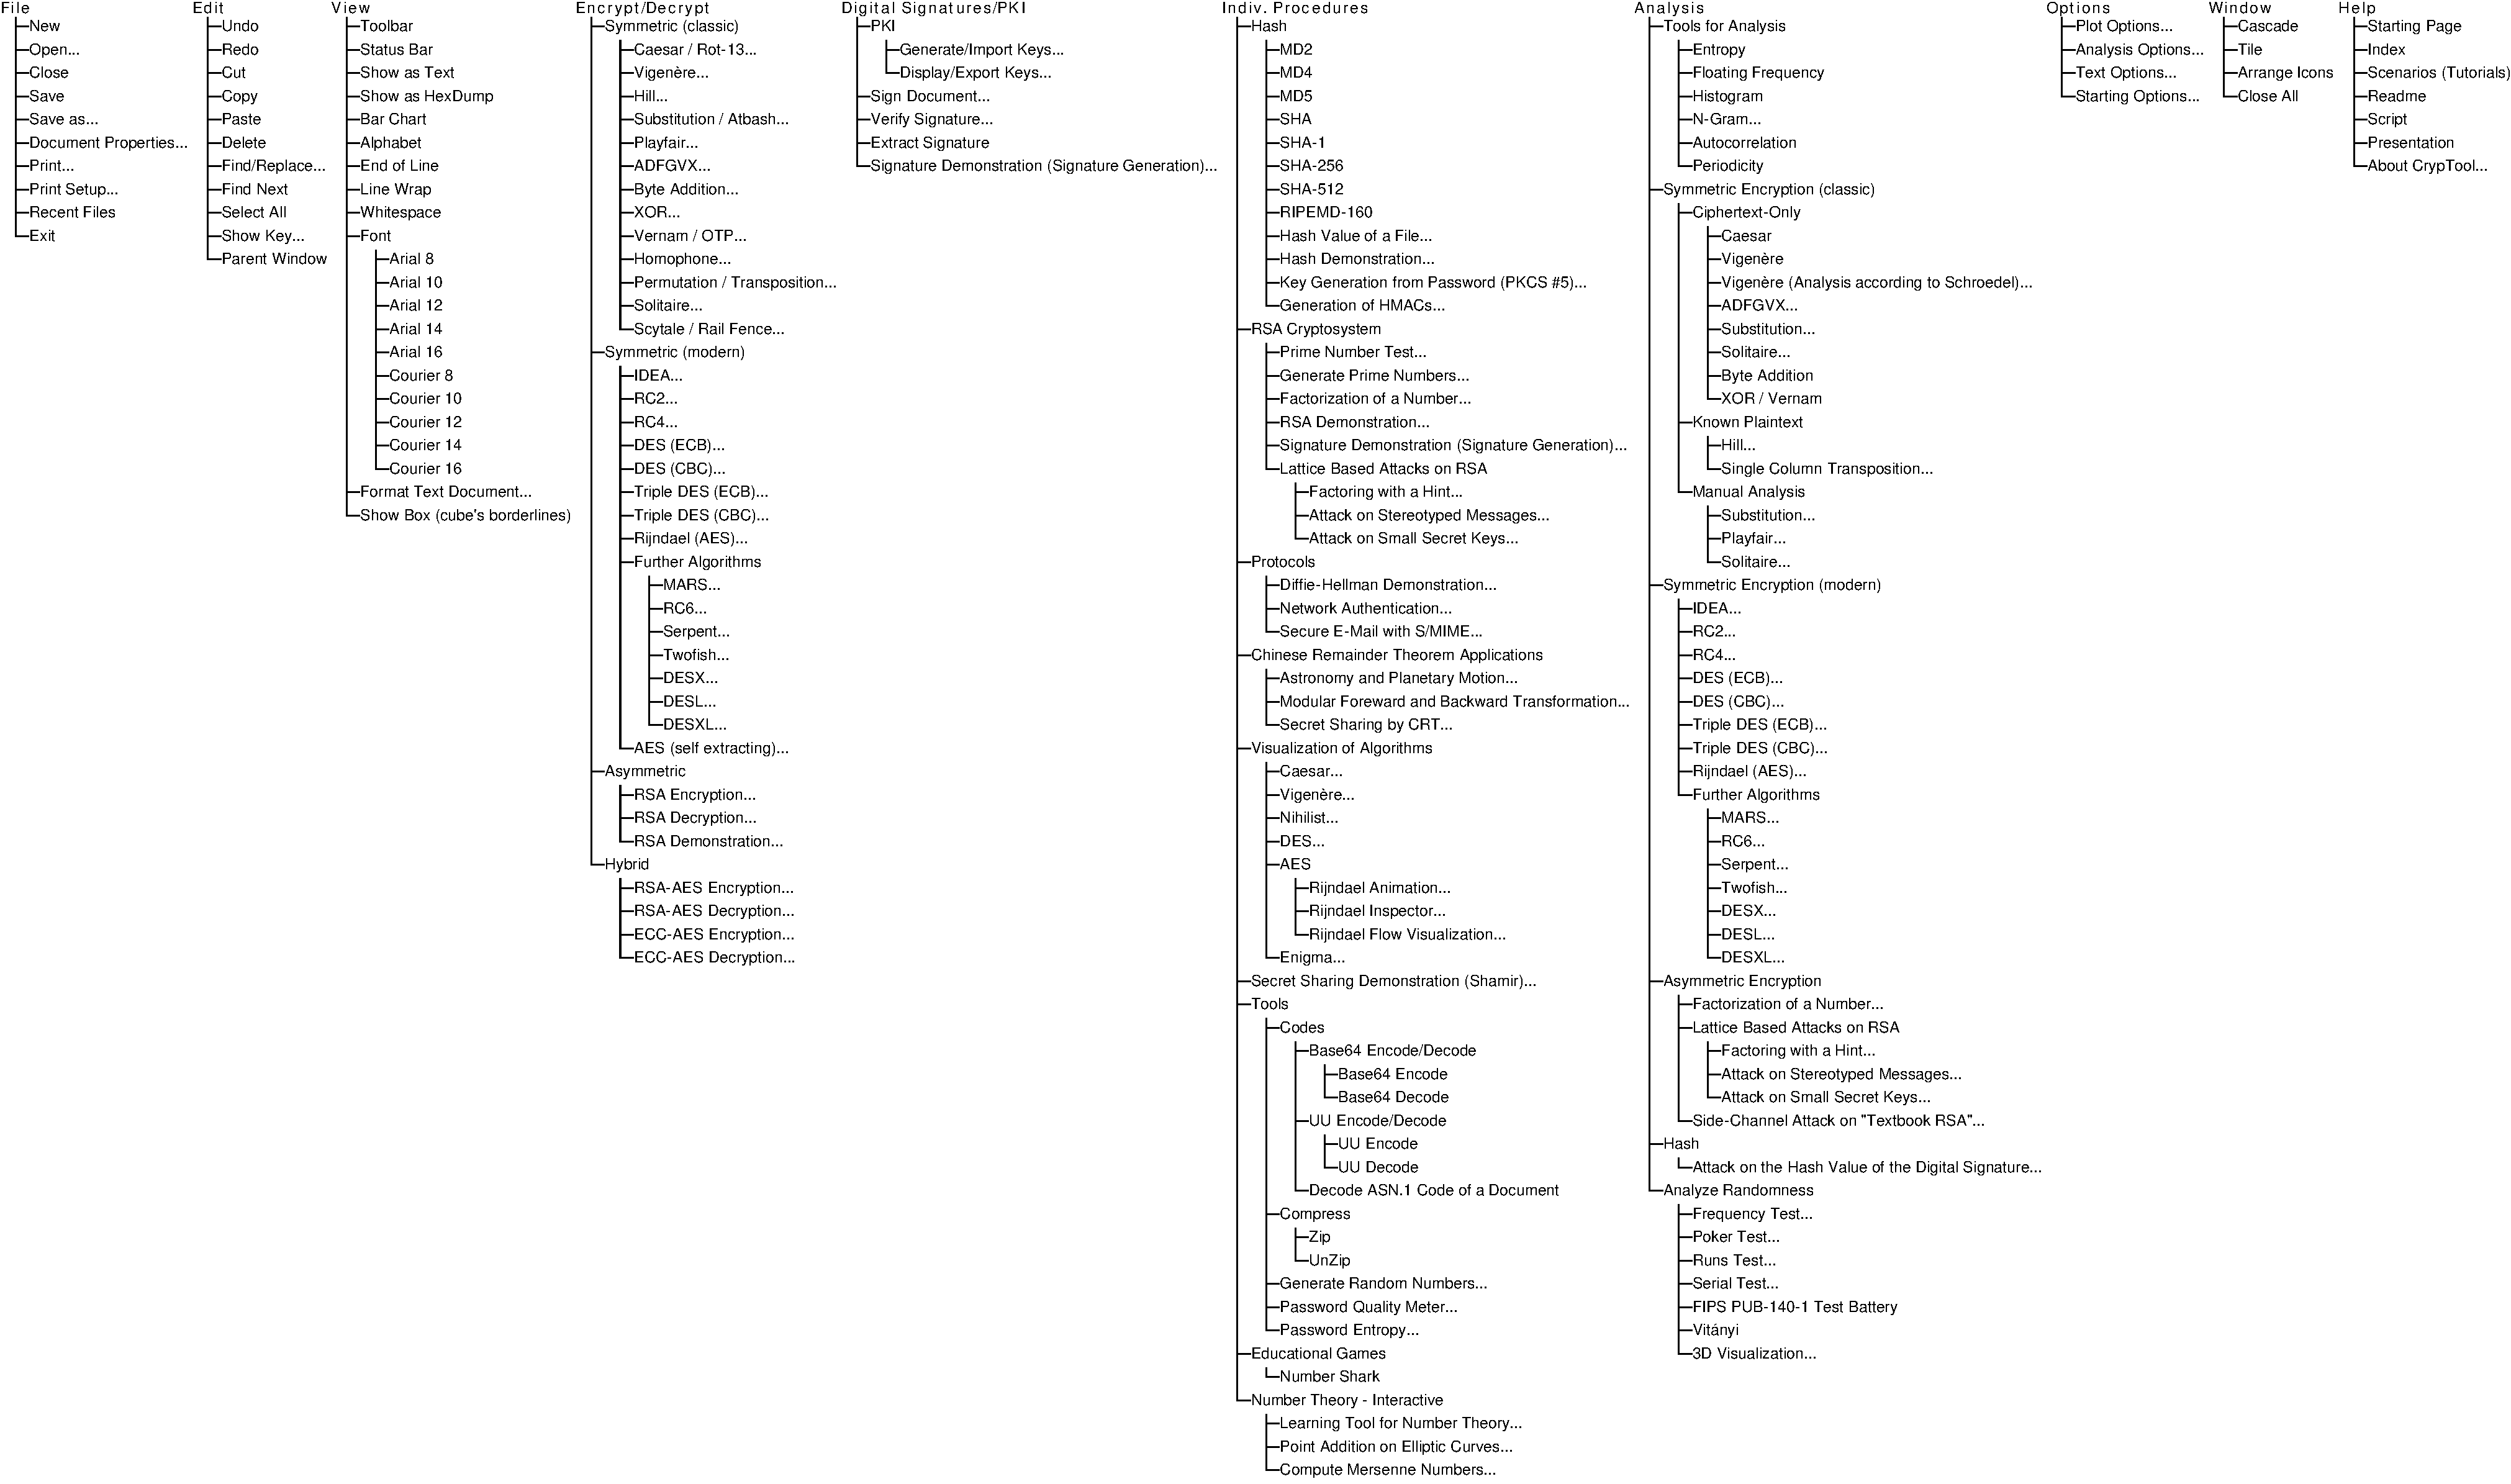
\includegraphics[scale=0.35]{figures/CT1-menutree-en}
\hypertarget{appendix-figure-menu-overview-CT1}{}
\caption{Complete overview of the menu tree of CT1 (CrypTool 1.4.31xxxxxxxxxxxxxxxxxxx)} 
\label{appendix-figure-menu-overview-CT1}
\end{minipage}
}
\end{center}
\end{figure}
\clearpage




%--------------------------------------------------------------------
\newpage
%\enlargethispage{1cm}
\hypertarget{appendix-template-overview-CT2}{}
\section{CrypTool 2 Templates}
\label{s:appendix-template-overview-CT2}

\noindent This appendix contains on the following pages the complete tree with
all templates in CT2\index{CrypTool 2}.\footnote{%
  You can find further information about CT2 at:
  \url{http://www.cryptool.org/en/ct2-documentation-en}
}

\noindent When you start CT2 it first shows the Startcenter.

%\clearpage
\begin{figure}[hb]
\begin{center}
%\vspace{-30pt}
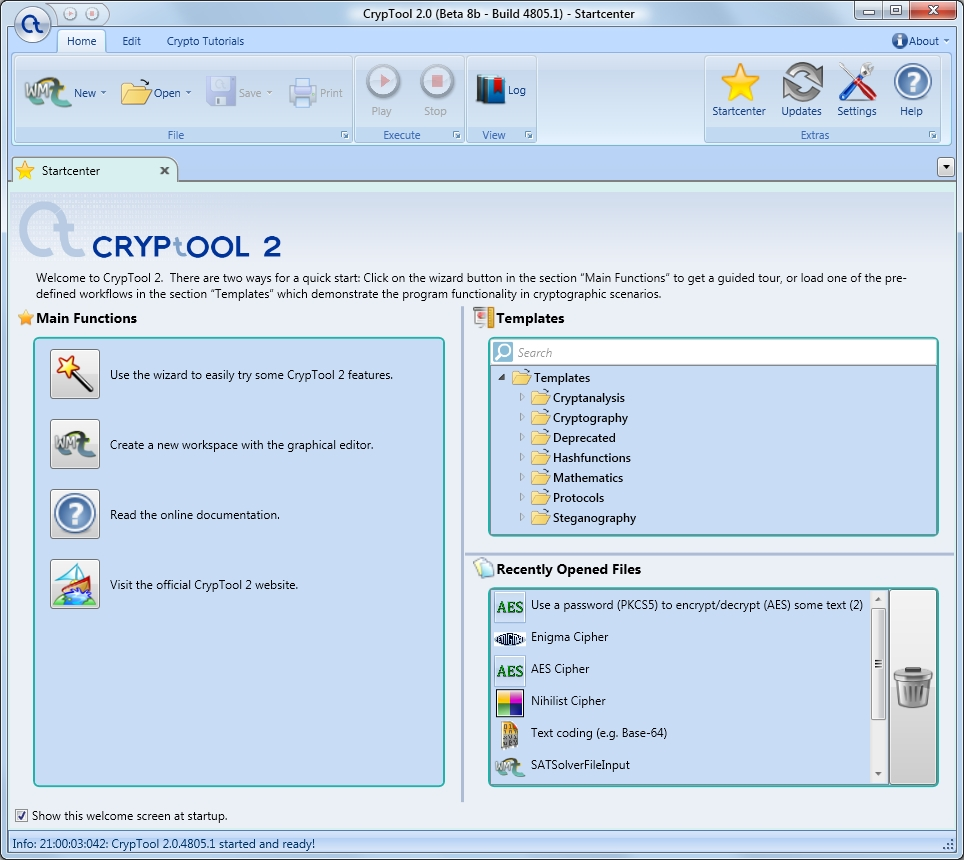
\includegraphics[scale=0.45, angle=0] {figures/CT2-Startcenter-en}
\hypertarget{Welcome-CT2}{}
\caption{Startcenter in CT2 (Beta 8b, May 2012)} 
\label{Welcome-Screenshot-CT2}
\end{center}
\end{figure}
%\clearpage

\noindent Within the Startcenter you have three main ways to use the implemented functionality:
\begin{itemize}
   \item via the Wizard, which leads you to the functions.
   \item via the Workspace, where you can compose the components (e.g. an encryption method, a text input function, ...)  by yourself according to the visual programming\index{visual programming} concept.
   \item via the template tree, which offers ready-to-run workflows.
 \end{itemize}

The Wizard asks questions so you can get to the desired scenarios (e.g. base64 coding) and then runs the according functions. You can afterwards save the chosen scenario as a normal template including the entries you used.

The empty workspace allows to drag on it any component from the navigation bar on the left and connect these components in the way you like. Most of the crypto functionality implemented in CT2 is offered using these components (e.g. Enigma, AES). 

The template tree contains at least one template for each implemented component. The offered templates contain read-to-run workflows. If you change e.g. within the AES template your input, you can see at once, how the output is modified dynamically (e.g. adding another block via padding, influence of the chosen chaining, ...).

\clearpage
\begin{figure}[hb]
\begin{center}
\vspace{-30pt}
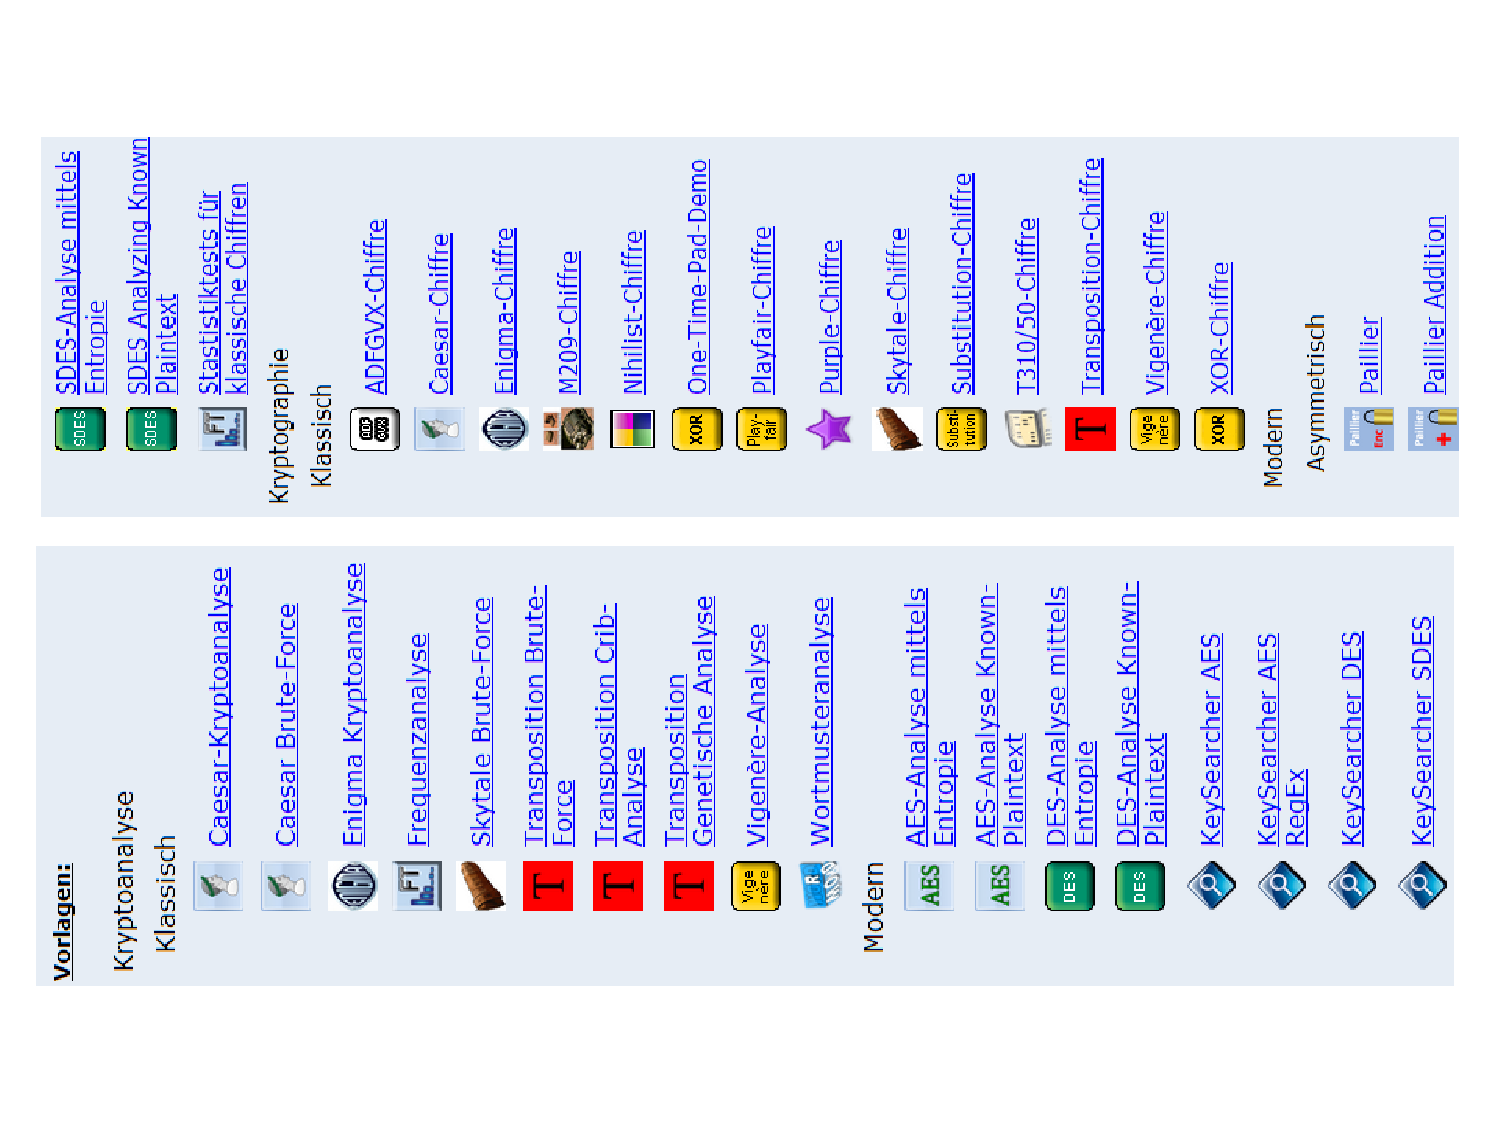
\includegraphics[scale=0.8, angle=270]
                {figures/CT2-templatetree-en-1}
\hypertarget{appendix-figure-template-overview-CT2}{}
\caption{Screenshot of the template tree of CT2 (NB4882.1, July 2012), Part 1} 
\label{appendix-figure-template-overview-CT2}
\end{center}
\end{figure}
\clearpage





%--------------------------------------------------------------------
\newpage
%\enlargethispage{1cm}
\hypertarget{appendix-function-overview-JCT}{}
\section{JCrypTool Functions}
\label{s:appendix-function-overview-JCT}

\noindent On the following pages this appendix contains a list of all
functions in JCrypTool\index{JCrypTool}.\footnote{%
  You can find further information about JCT at:
  \url{http://www.cryptool.org/en/jct-volunteer-en} \\
  This list was generated using the CT Portal website.}

\noindent When you start JCT the first time it shows the Welcome window.

%\clearpage
\begin{figure}[hb]
\begin{center}
%\vspace{-30pt}
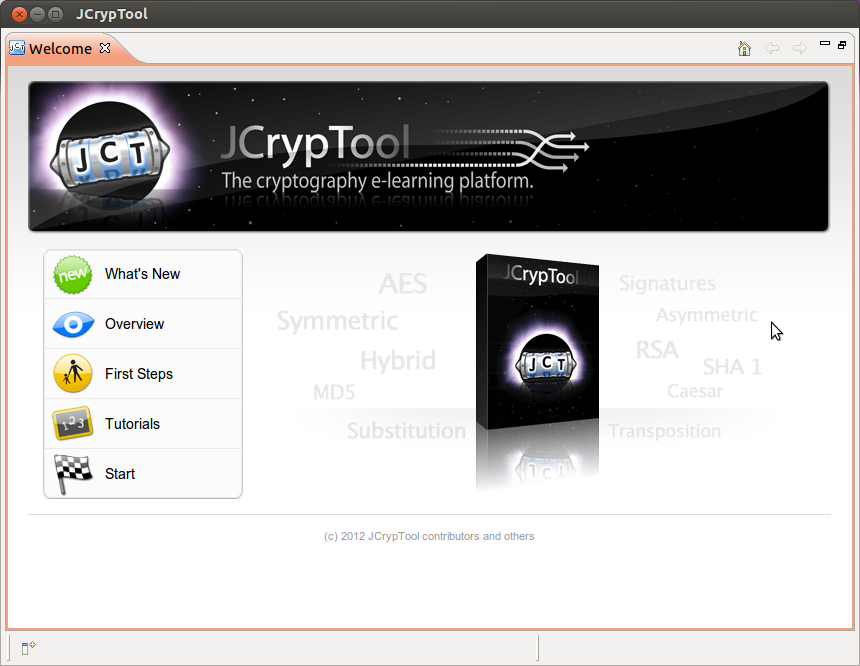
\includegraphics[scale=0.45, angle=0] {figures/JCT-Welcome-EN}
\hypertarget{Welcome-Screenshot-JCT}{}
\caption{Welcome screenshot in JCT (RC6, July 2012)} 
\label{Welcome-Screenshot-JCT}
\end{center}
\end{figure}
%\clearpage
After pressing ``Start'' you can directly use the different functions.
The functions implemented in JCT are presented in two different perspectives:
\begin{itemize}
   \item Default Perspective
   \item Algorithm Perspective
 \end{itemize}

All functions of the {\bf Default Perspective} can be found both in the menus and in the navigation bar called ``Crypto Explorer'' (at the right side).
The Default Perspective contains all important methods like classic transposition or modern AES, and many visualizations (e.g. Diffie-Hellman key exchange or caculations on elliptic curves).

All functions of the {\bf Algorithm Perspective} can be found in the navigation bar called ``Algorithms'' (in this perspective also at the right side).
The Algorithm Perspective contains all detail settings of the various algorithms, it especially offers post-quantum computing algorithms\index{post-quantum computing}\index{PQC}.

\clearpage
\begin{figure}[hb]
\begin{center}
\vspace{-30pt}
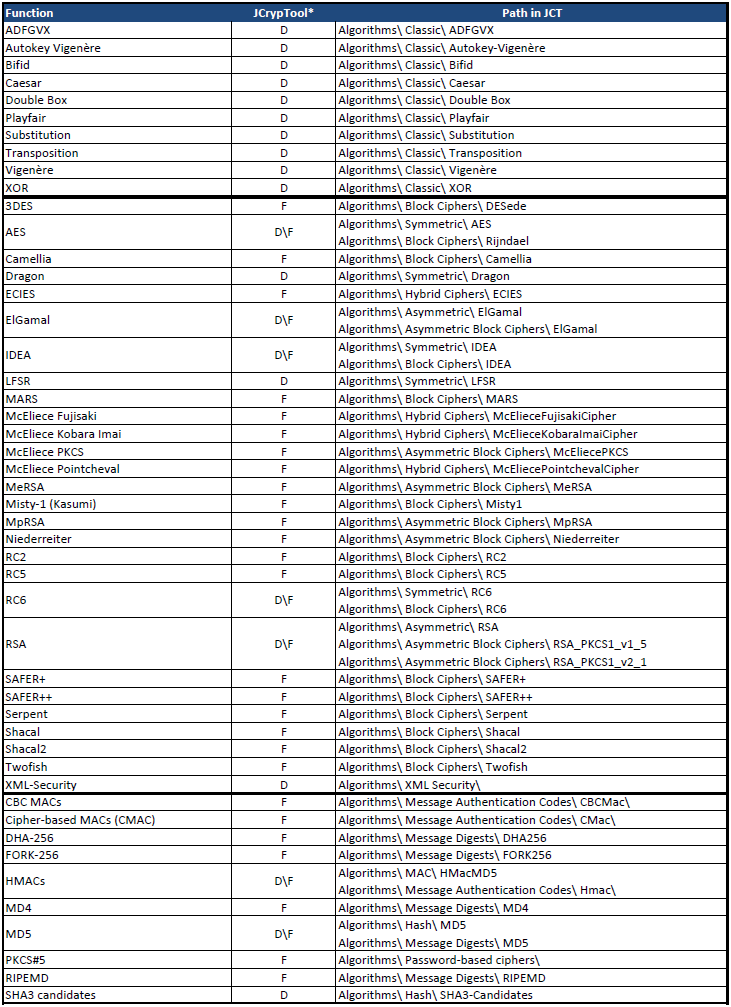
\includegraphics[scale=0.8, angle=0] {figures/JCT-functions-en-1}
\hypertarget{functions-overview-1-JCT}{}
\caption{Screenshot of the functions of JCT (RC6, July 2012), Part 1} 
\label{functions-overview-1-JCT}
\end{center}
\end{figure}
\clearpage

\clearpage
\begin{figure}[hb]
\begin{center}
\vspace{-30pt}
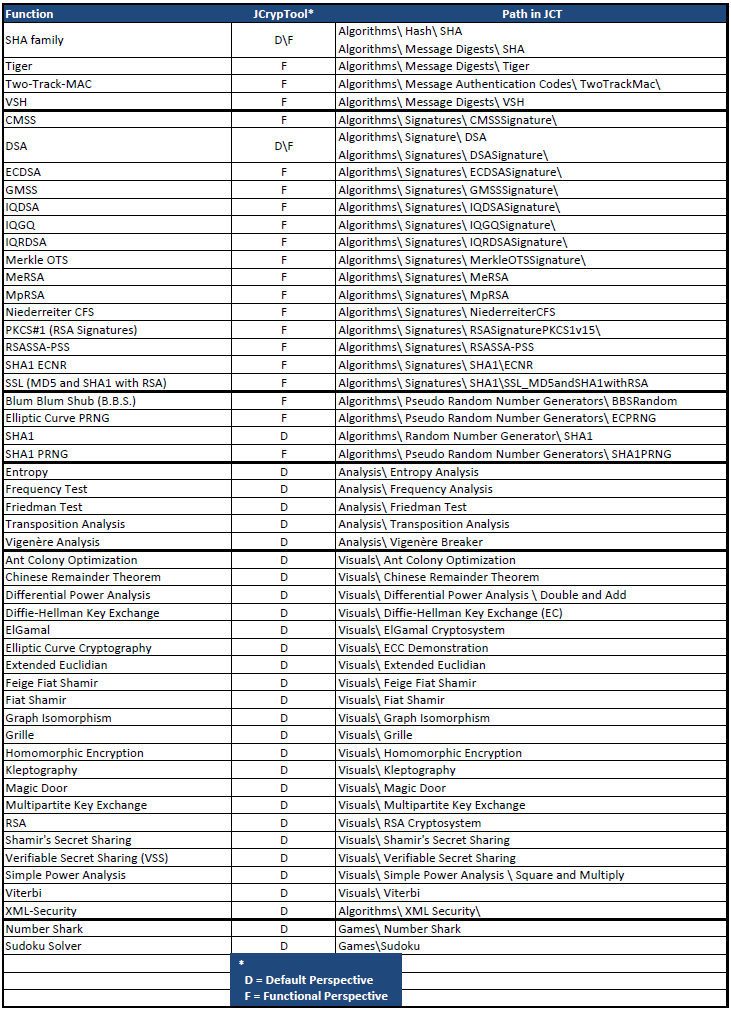
\includegraphics[scale=0.8, angle=0] {figures/JCT-functions-en-2}
\hypertarget{functions-overview-2-JCT}{}
\caption{Screenshot of the functions of JCT (RC6, July 2012), Part 2} 
\label{functions-overview-2-JCT}
\end{center}
\end{figure}
\clearpage





%--------------------------------------------------------------------
\newpage
%\enlargethispage{1cm}
\hypertarget{appendix-function-overview-CTO}{}
\section{CrypTool-Online Functions}
\label{s:appendix-function-overview-CTO}

\noindent This appendix contains a list of all
functions in CrypTool-Online (CTO)\index{CrypTool-Online}.\footnote{%
  You can find further information about CTO at:
  \url{www.cryptool-online.org} \\
  This list was generated using the functions list at the CT Portal website:\\
  \url{http://www.cryptool.org/ctp-documentation-en/ctp-functions-en}}


%\noindent The starting page of CTO looks like this:
%\begin{figure}[hb]
%\begin{center}
%\vspace{-30pt}
%\includegraphics[scale=0.45, angle=0] {figures/CTO-Welcome-EN}
%\hypertarget{Welcome-Screenshot-CTO}{}
%\caption{Welcome screenshot in CrypTool-Online (November 2012)} 
%\label{Welcome-Screenshot-CTO}
%\end{center}
%\end{figure}


\noindent The following screenshot shows the crypto functions implemented on CTO:
\clearpage
\begin{figure}[hb]
\begin{center}
\vspace{-30pt}
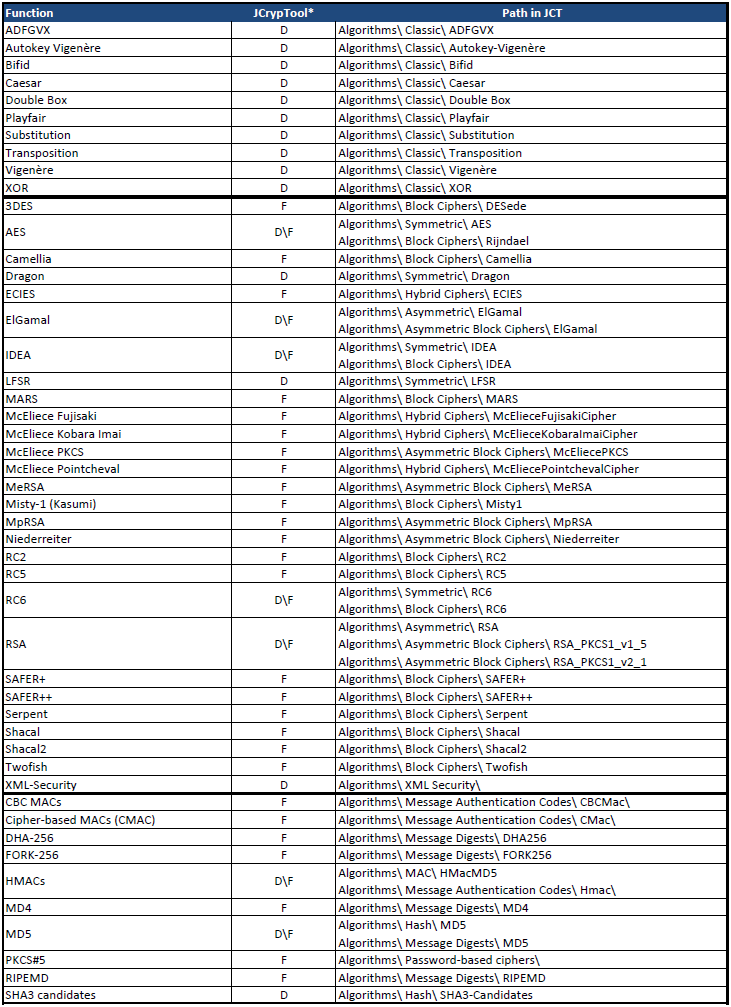
\includegraphics[scale=0.8, angle=0] {figures/JCT-functions-en-1}
\hypertarget{functions-overview-1-CTO}{}
\caption{Screenshot of the functions of CTO (November 2012)} 
\label{functions-overview-1-CTO}
\end{center}
\end{figure}
\clearpage

%\clearpage
%\begin{figure}[hb]
%\begin{center}
%\vspace{-30pt}
%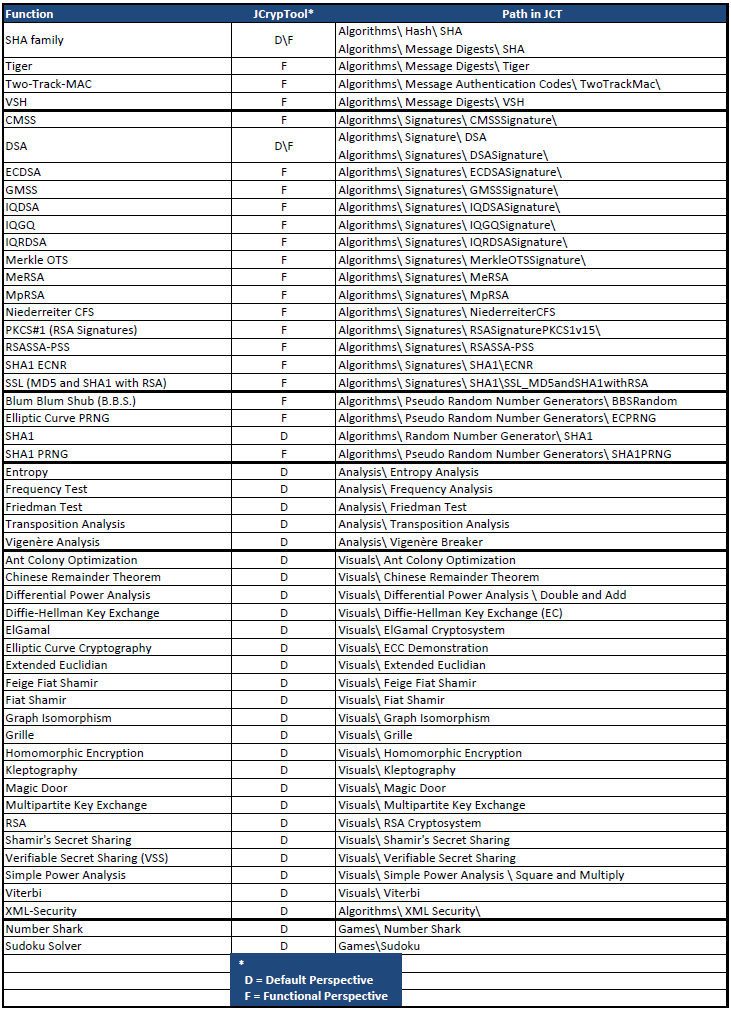
\includegraphics[scale=0.8, angle=0] {figures/JCT-functions-en-2}
%\hypertarget{functions-overview-2-CTO}{}
%\caption{Screenshot of the functions of CTO (November 2012), Part 2} 
%\label{functions-overview-2-CTO}
%\end{center}
%\end{figure}
%\clearpage


  
% ++++++++++++++++++++++++++++++++++++++++++++++++++++++++++++++++++++++++++
\newpage
\hypertarget{appendix-movies}{}
\section{Filme und belletristische Literatur mit Bezug zur Kryptographie}
\label{s:appendix-movies}  
% {\bf Filme und Literatur mit Bezug zur Kryptographie} (siehe Anhang \ref{s:appendix-movies})
\index{Filme}
\index{Literatur}


Kryptographische Verfahren -- sowohl klassische wie moderne -- fanden auch
Eingang in die Literatur und in Filme. In manchen Medien werden diese nur
erw�hnt und sind reine Beigabe, in anderen sind sie tragend und werden
genau erl�utert, und manchmal ist die Rahmenhandlung nur dazu da, dieses
Wissen motivierend zu transportieren. Anbei der Beginn eines �berblicks.

% --------------------------------------------------------------------------
\subsection{F�r Erwachsene und Jugendliche}

%be_2005: Hatte zuerst \begin{thebibliography}{99999} und \bibitem[... ,
%         aber dann wurde immer der feste Titel "Literatur" bzw. "References"
%         geschrieben und wir fanden keine M�glichkeit, ihn weg zu bekommen.
%         L�sung: Stattdessen \begin{description} \item[...


\begin{description}

\item[\textrm{[Poe1843]}] \index{Poe 1843}
    Edgar Allan Poe\index{Poe, Edgar Allan}, \\
    {\em Der Goldk�fer}, 1843. \\
    Diese Kurzgeschichte erschien in Deutsch z.B. in der illustrierten und
    mit Kommentaren in den Marginalspalten versehenen Ausgabe "`Der Goldk�fer
    und andere Erz�hlungen"', Gerstenbergs visuelle Weltliteratur,
    Gerstenberg Verlag, Hildesheim, 2002.\\
    In dieser Kurzgeschichte beschreibt Poe als Ich-Erz�hler seine
    Bekanntschaft mit dem sonderbaren Legrand. Mit Hilfe eines an der
    K�ste Neuenglands gefundenen Goldk�fers, einem alten Pergament und
    den Dechiffrierk�nsten von Legrand finden Sie den sagenhaften Schatz
    von Kapit�n Kidd.\\
    Die Geheimschrift besteht aus 203 kryptischen Zeichen und erweist sich
    als allgemeine monoalphabetische Substitutions-Chiffre (vgl. 
    Kapitel~\ref{monoalphabeticSubstitutionCiphers}). Ihre schrittweise 
    Dechiffrie"-rung durch semantische und syntaktische Analyse
    (H�ufigkeiten der einzelnen Buchstaben in englischen Texten)
    wird ausf�hrlich erl�utert.\\
    Der Entschl�sseler Legrand sagt darin (S. 39) den ber�hmten Satz:
    "`Und es ist wohl sehr zu bezweifeln, ob menschlicher Scharfsinn
    ein R�tsel ersinnen kann, das menschlicher Scharfsinn bei
    entsprechender Hingabe nicht wieder zu l�sen vermag."'\\
    % D: Poe: 1809-1849, "Vater des Kriminalromans", er schloss Wetten ab,
    % dass er alle verschl�sselten Botschaften, die ihm Freunde und Leser
    % vorlegten, im Handumdrehen entschl�sseln k�nne. Gutes Gesp�r durch
    % viel �bung.
    % E: Poe, 1809-1849 was named "Father of the crime novel". He claimed,
    % that he will be able to decrypt any cipher sent to him by friends or
    % readers.
 
    % Originalausgabe dieser illustrierten Ausgabe: "Le scarab�e d'or et 
    %                           autre nouvelles", Gallimard, Paris, 1998.
    % In "Der Goldk�fer" wird detailliert beschrieben, wie der verarmte
    % Hugenotte William Legrand in South Carolina die monoalphabetische
    % Geheimschrift des Piratenkapit�ns Kidd knackt, die zu einem
    % sagenhaften Schatz f�hrt.


\item[\textrm{[Verne1885]}] \index{Verne 1885}
    Jules Verne\index{Verne, Jules}, \\
    {\em Mathias Sandorf}, 1885. \\
    Dies ist einer der bekanntesten Romane des franz�sischen Schriftstellers
    Jules Verne (1828-1905), der auch als "`Vater der Science Fiction"'
    bezeichnet wurde.\\
    Erz�hlt wird die spannende Geschichte des Freiheitsk�mpfers Graf
    Sandorf, der an die Polizei verraten wird, aber schlie�lich fliehen
    kann.\\
    M�glich wurde der Verrat nur, weil seine Feinde eine Geheimbotschaft an
    ihn abfangen und entschl�sseln konnten. Dazu ben�tigten sie eine
    besondere Schablone, die sie ihm stahlen. Diese Schablone bestand aus
    einem quadratischen St�ck Karton mit 6x6 K�stchen, wovon 1/4, also neun,
    ausgeschnitten waren (vgl. die
    \hyperlink{turning-grille}{Flei�ner-Schablone}
    in Kapitel~\ref{introsamplesTranspositionCiphers}).\\


    % Gefunden in: CRYPTO-GRAM, January 15, 2007, by Bruce Schneier
\item[\textrm{[Kipling1901]}] \index{Kipling 1901}
    Rudyard Kipling\index{Kipling, Rudyard}, \\
    {\em Kim}, 1901. \\
    Dieser Roman wird in der Besprechung von Rob Slade%
    \footnote{Siehe
      % \href{http://catless.ncl.ac.uk/Risks/24.49.html\#subj12} %% \ vor # n�tig !
        \url{http://catless.ncl.ac.uk/Risks/24.49.html#subj12}.
    }
    folgenderma�en beschrieben:
    "`Kipling packte viele Informationen und Konzepte in seine Geschichten.
    In "`Kim"' geht es um das gro�e "`Spiel"' Spionage und Bespitzelung.
    Schon auf den ersten 20 Seite finden sich Authentisierung �ber Besitz,
    Denial of Service, Sich-f�r-jemand-anderen-Ausgeben (Impersonation),
    Heimlichkeit, Maskerade, Rollen-basierte Autorisierung (mit 
    Ad-hoc-Authentisierung durch Wissen), Abh�ren, und Vertrauen basierend
    auf Datenintegrit�t.
    Sp�ter kommen noch Contingency Planning gegen Diebstahl und
    Kryptographie mit Schl�sselwechsel hinzu."'\\
    Das Copyright des Buches ist abgelaufen%
    \footnote{Sie k�nnen es lesen unter:\\
          \url{http://whitewolf.newcastle.edu.au/words/authors/K/KiplingRudyard/prose/Kim/index.html},\\
          \url{http://kipling.thefreelibrary.com/Kim} oder\\
          \url{http://www.readprint.com/work-935/Rudyard-Kipling}.
    }.\\


\item[\textrm{[Doyle1905]}] \index{Doyle 1905}
    Arthur Conan Doyle\index{Doyle, Sir Arthur Conan}, \\
    {\em Die tanzenden M�nnchen}, 1905. \\
    In der Sherlock-Holmes-Erz�hlung {\em Die tanzenden M�nnchen} 
    (erschienen erstmals 1903 im "`Strand Magazine"', und dann 1905 im 
    Sammelband "`Die R�ckkehr des Sherlock Holmes"' erstmals in Buchform)
    wird Sherlock Holmes mit einer Geheimschrift konfrontiert, die zun�chst
    wie eine harmlose Kinderzeichnung aussieht. \\
    Sie erweist sich als monoalphabetische Substitutions-Chiffre (vgl. 
    Kapitel~\ref{monoalphabeticSubstitutionCiphers}) des Verbrechers Abe
    Slaney. Holmes knackt die Geheimschrift mittels H�ufigkeitsanaly"-se.\\


\item[\textrm{[Sayers1932]}] \index{Sayers 1932}
    Dorothy L. Sayers, \\
    {\em Zur fraglichen Stunde und Der Fund in den Teufelsklippen 
    (Orginaltitel: Have his carcase)}, Harper, 1932 \\
    (1. dt. �bersetzung {\em Mein Hobby: Mord} bei A. Scherz, 1964; \\
    dann {\em Der Fund in den Teufelsklippen} bei Rainer Wunderlich-Verlag, 
    1974;\\
    Neu�bersetzung 1980 im Rowohlt-Verlag). \\
    In diesem Roman findet die Schriftstellerin Harriet Vane eine Leiche 
    am Strand und die Polizei h�lt den Tod f�r einen Selbstmord. 
    Doch Harriet Vane und der elegante Amateurdetektiv Lord Peter Wimsey
    kl�ren in diesem zweiten von Sayers's ber�hmten Harriet Vane's
    Geschichten den widerlichen Mord auf. \\
    Dazu ist ein Chiffrat zu l�sen. Erstaunlicherweise beschreibt der
    Roman nicht nur detailliert die Playfair-Chiffre, sondern auch deren
    Kryptoanalyse (vgl. \hyperlink{playfair}{Playfair}
    in Kapitel~\ref{polygraphicSubstitutionCiphers}).\\


\item[\textrm{[Simmel1970]}] \index{Simmel 1970}
    Johannes Mario Simmel, \\
    {\em Und Jimmy ging zum Regenbogen}, Knaur Verlag, 1970. \\
    Der Roman spielt zwischen 1938 und
    1969 in Wien. Der Held Manuel Aranda deckt -- von mehreren Geheimdiensten
    verfolgt -- im Laufe der Handlung St�ck f�r St�ck die Vergangenheit seines
    ermordeten Vaters auf. Ein wichtiger Mosaikstein ist dabei ein
    verschl�sseltes Manuskript, das in Kapitel 33 entschl�ssselt wird. 
    Im Roman wird der Code als ein
    "`f�nfundzwanzigfacher Caesar Code"' beschrieben, tats�chlich ist es eine
    Vigen�re-Chiffre mit einem 25 Buchstaben langen Schl�ssel. \\
    Das Buch wurde 1971 verfilmt.\\


\item[\textrm{[Crichton1988]}] \index{Crichton 1988}
    Michael Crichton, \\
    {\em Die Gedanken des B�sen (Orginaltitel: Sphere)}, Rororo, 1988. \\
    Ein Team verschiedener Wissenschaftler wird auf den Meeresgrund geschickt, 
    um ein 900~m langes hoch entwickeltes Raumschiff zu untersuchen. Die 
    Eigenheiten und psychischen Probleme der Forscher treten durch lebensbedrohliche 
    Ereignisse und ihr Abgeschnittensein von oben immer mehr in den Vordergrund. 
    Es gibt viele R�tsel: Das Raumschiff liegt schon 300 Jahre da, es hat 
    englische Beschriftungen, es f�hrt scheinbar ein Eigenleben, die menschliche 
    Vorstellungskraft materialisiert sich. Unter anderem erscheint auf dem
    Bildschirm ein im Buch vollst�ndig abgedruckter Code, der von dem genialen
    Mathematiker Harry entschl�sselt werden kann: ein einfacher spiralenf�rmiger
    Ersetzungscode.\\

    
\item[\textrm{[Seed1990]}] \index{Seed 1990}
    Regie Paul Seed (Paul Lessac), \\
    {\em Das Kartenhaus (Orginaltitel: House of Cards)}, 1990 (dt. 1992). \\
    In diesem Film versucht Ruth, hinter das Geheimnis zu kommen, das ihre
    Tochter verstummen lie�. Hierin unterhalten sich Autisten mit Hilfe von
    5- und 6-stelligen Primzahlen (siehe 
    Kapitel~\ref{Label_Kapitel_Primes}).
    Nach �ber eine Stunde kommen im Film die folgenden beiden (nicht
    entschl�sselten) Primzahlfolgen vor:
%  \vskip -30pt  %be_2005 Bewirkt anscheinend nichts -- Abstand etwas zu gro�.
    \begin{center}
    $21.383, \;\;176.081, \;\;18.199, \;\;113.933, \;\;150.377, \;\;304.523, \;\;113.933$\\
    $193.877, \;\;737.683, \;\;117.881, \;\;193.877$
    \end{center}
    \vskip +10 pt   % da "\\" hier nicht geht!


\item[\textrm{[Robinson1992]}] \index{Robinson 1992}
    Regie Phil Alden Robinson, \\
    {\em Sneakers - Die Lautlosen (Orginaltitel: Sneakers)},
    Universal Pictures Film, 1992. \\
    In diesem Film versuchen die "`Sneakers"' (Computerfreaks um ihren Boss
    Martin Bishop), den "`B�sen"' das Dechiffrierungsprogramm SETEC abzujagen.
    SETEC wurde von einem genialen Mathematiker vor seinem gewaltsamen Tod
    erfunden und kann alle Geheimcodes dieser Welt entschl�sseln.\\
    In dem Film wird das Verfahren nicht beschrieben%
    \footnote{
       An dem Film hatte Leonard Adleman (das "`A"' von RSA) als mathematischer
       Berater mitgearbeitet. Die recht lustige Geschichte �ber seine Mitwirkung
       bei Sneakers beschreibt er selbst auf seiner Homepage unter
       \url{http://www.usc.edu/dept/molecular-science/fm-sneakers.htm}.
       Man kann man davon ausgehen, dass es sich bei dem �berall benutzten
       Verschl�sselungsverfahren um RSA handelt.      
       In dem Chip ist demnach ein bis dahin unbekanntes, schnelles 
       Faktorisierungsverfahren\index{Faktorisierung} implementiert.
    }.\\


\item[\textrm{[Baldacci1997]}] \index{Baldacci 1997}
    David Baldacci, \\
    {\em Das Labyrinth. Total Control}, L�bbe, 1997. \\
    Jason Archer, Direktor einer Technologie-Firma, verschwindet pl�tzlich.
    Seine Frau Sidney Archer versucht, den Grund seines pl�tzlichen Todes
    herauszufinden, und entdeckt, wie das Finanzsystem missbraucht wird und
    dass die reale Macht bei denen mit dem meisten Geld liegt. Hier helfen
    dann auch gute Passworte nicht...\\


\item[\textrm{[Natali1997]}] \index{Natali 1997}
    Regie Vincenzo Natali, \\
    {\em Cube (Orginaltitel: Sneakers)},
    Mehra Meh Film, 1997. \\
    In diesem kanadischen Low-Budget-Film finden sich 7 sehr unterschiedliche
    Personen in einem endlos scheinenden Labyrinth von w�rfelartigen R�umen.\\
    Die Personen wollen nach drau�en, m�ssen dazu aber die R�ume durchqueren,
    von denen manche t�dliche Fallen darstellen. Um herauszufinden, welche
    R�ume gef�hrlich sind, spielt Mathematik eine entscheidende Rolle: Jeder
    Raum hat am Eingang eine Folge von 3 mal 3 Ziffern. Zuerst nehmen
    sie an, dass alle R�ume Fallen sind, wo wenigstens eine der 3 Zahlen eine
    Primzahl ist. Sp�ter stellt sich heraus, dass auch alle diejenigen R�ume
    Fallen sind, bei denen eine der 3 Zahlen eine Potenz von genau einer
    Primzahl ist (Fallen sind also $p^n$, z.B. $128=2^7$ oder
    $101 = 101^1 = prim$, aber nicht $517 = 11*47$).\\


\item[\textrm{[Becker1998]}] \index{Becker 1998}
    Regie Harold Becker, \\
    {\em Das Mercury Puzzle (Orginaltitel: Mercury Rising)}, 
    Universal Pictures Film, 1998. \\
    Die NSA hat einen neuen Code entwickelt, der angeblich weder von Menschen
    noch von Computern geknackt werden kann. Um die Zuverl�ssigkeit zu testen,
    verstecken die Programmierer eine damit verschl�sselte Botschaft in
    einem R�tselheft.\\
    Simon, eine neunj�hriger autistischer Junge, knackt den Code.
    Statt den Code zu fixen, schickt ihm ein Sicherheitsbeamter einen Killer.
    Der FBI-Agent Art Jeffries (Bruce Willis) besch�tzt den Jungen und
    stellt den Killern eine Falle.\\    
    Das Chiffrier-Verfahren wird nicht beschrieben.\\


\item[\textrm{[Brown1998]}] \index{Brown 1998}
    Dan Brown, \\
    {\em Diabolus (Orginaltitel: Digital Fortress)}, L�bbe, 2005. \\
    Dan Browns erster Roman "`The Digital Fortress"' erschien 1998 als E-Book,
    blieb jedoch damals weitgehend erfolglos.\\
    Die National Security Agency (NSA) hat f�r mehrere Milliarden US-Dollar
    einen gewaltigen Computer gebaut, mit dem sie in der Lage ist, auch nach
    modernsten Verfahren verschl�sselte Meldungen (nat�rlich nur die von
    Terroristen und Verbrechern) innerhalb weniger Minuten zu entziffern.\\
    Ein abtr�nniger Angestellter erfindet einen unbrechbaren Code und
    sein Computerprogramm Diabolus zwingt damit den Supercomputer zu
    selbstzerst�rerischen Rechenoperationen. Der Plot, in dem auch die
    sch�ne Computerexpertin Susan Fletcher eine Rolle spielt, ist ziemlich
    vorhersehbar.\\
    Die Idee, dass die NSA oder andere Geheimdienste jeden Code knacken
    k�nnen, wurde schon von mehreren Autoren behandelt: Hier hat der
    Supercomputer 3 Millionen Prozessoren -- trotzdem ist es aus heutiger
    Sicht damit auch nicht ann�herungsweise m�glich, diese modernen Codes
    zu knacken.\\


\item[\textrm{[Elsner1999]}] \index{Elsner 1999}
    Dr.~C.~Elsner, \\
    {\em Der Dialog der Schwestern}, c't, Heise-Verlag, 1999. \\
    In dieser Geschichte, die dem CrypTool-Paket\index{CrypTool} als PDF-Datei
    beigelegt ist, unterhalten sich die Heldinnen vertraulich mit einer
    Variante des RSA-Verfahrens (vgl. Kapitel~\ref{rsabeweis} ff.).
    Sie befinden sich in einem Irrenhaus unter st�ndiger Bewachung.\\
    

\item[\textrm{[Stephenson1999]}] \index{Stephenson 1999}
    Neal Stephenson, \\
    {\em Cryptonomicon}, Harper, 1999. \\
    Der sehr dicke Roman besch�ftigt sich mit Kryptographie sowohl im 
    zweiten Weltkrieg als auch in der Gegenwart.
    Die zwei Helden aus den 40er-Jahren sind der gl�nzende Mathematiker und
    Kryptoanalytiker Lawrence Waterhouse, und der �bereifrige,
    morphiums�chtige Bobby Shaftoe von den US-Marines. 
    Sie geh�ren zum Sonderkommando 2702, einer Alliiertengruppe, die
    versucht, die gegnerischen Kommunikationscodes zu knacken und dabei
    ihre eigene Existenz geheim zu halten. \\
    In der Gegenwartshandlung tun sich die Enkel der Weltkriegshelden -- der
    Programmierfreak Randy Waterhouse und die sch�ne Amy Shaftoe -- zusammen. \\
    Cryptonomicon ist f�r nicht-technische Leser teilweise schwierig zu
    lesen. Mehrere Seiten erkl�ren detailliert Konzepte der Kryptographie.
    Stephenson legt eine ausf�hrliche Beschreibung der Solitaire-Chiffre
    (siehe Kapitel~\ref{Further-PaP-methods}) bei, ein 
    Papier- und Bleistiftverfahren\index{Papier- und Bleistiftverfahren},
    das von Bruce Schneier entwickelt wurde und im
    Roman "`Pontifex"' genannt wird. Ein anderer, moderner Algorithmus
    namens "`Arethusa"' wird dagegen nicht offengelegt.\\


\item[\textrm{[Elsner2001]}] \index{Elsner 2001}
    Dr.~C.~Elsner, \nopagebreak\\
    {\em Das Chinesische Labyrinth}, c't, Heise-Verlag, 2001. \\
    In dieser Geschichte, die dem CrypTool-Paket\index{CrypTool} als PDF-Datei
    beigelegt ist, muss Marco Polo in einem Wettbewerb Probleme aus der
    Zahlentheorie l�sen, um Berater des gro�en Khan zu werden. Alle L�sungen 
    sind angef�gt und erl�utert.\\


\item[\textrm{[Colfer2001]}] \index{Colfer 2001}
    Eoin Colfer, \\
    {\em Artemis Fowl}, List-Verlag, 2001. \\  
    In diesem Jugendbuch gelangt der junge Artemis, ein Genie und Meisterdieb,
    an eine Kopie des streng geheimen "`Buches der Elfen"'. Nachdem er es mit 
    Computerhilfe entschl�sselt hat, erf�hrt er Dinge, die kein Mensch
    erfahren d�rfte. \\
    Der Code wird in dem Buch nicht genauer beschrieben.\\


\item[\textrm{[Howard2001]}] \index{Howard 2001}
    Regie Ron Howard, \\
    {\em A Beautiful Mind}, 2001. \\
    Verfilmung der von Sylvia Nasar verfassten Biographie des
    Spieltheoretikers John Nash. 
    Nachdem der brillante, aber unsoziale Mathematiker geheime kryptographische
    Arbeiten annimmt, verwandelt sich sein Leben in einen Alptraum. Sein 
    unwiderstehlicher Drang, Probleme zu l�sen, gef�hrden ihn und sein 
    Privatleben.
    Nash ist in seiner Vorstellungswelt ein staatstragender Codeknacker. \\
    Konkrete Angaben zur seinen Analyseverfahren werden nicht beschrieben.\\


\item[\textrm{[Apted2001]}] \index{Apted 2001}
    Regie Michael Apted, \\
    {\em Enigma -- Das Geheimnis}, 2001. \\
    Verfilmung des von Robert Harris verfassten "`historischen Romans"' 
    {\em Enigma} (Hutchinson, London, 1995) �ber die ber�hmteste 
    Verschl�sselungsmaschine in der Geschichte, die in
    Bletchley Park nach polnischen Vorarbeiten gebrochen wurde. 
    Die Geschichte spielt 1943, als der eigentliche Erfinder Alan Turing
    schon in Amerika war. So kann der Mathematiker Tom Jericho als Hauptperson
    in einem spannenden Spionagethriller brillieren.\\
    Konkrete Angaben zu dem Analyseverfahren werden nicht gemacht.\\


\item[\textrm{[Isau2003]}] \index{Isau 1997}
    Ralf Isau, \\
    {\em Das Museum der gestohlenen Erinnerungen}, Thienemann-Verlag, 1997/2003. \\
    Ein sehr spannender, hervorragend recherchierter und doch leicht zu lesender
    Roman mit einem tiefen Hintersinn.\\
    Als die Zwillinge Oliver und Jessica von ihren Ferien zur�ckkommen, haben sie
    ihren Vater vergessen. Die Realit�t verschiebt sich und niemand scheint es zu
    bemerken. An einigen Stellen bleiben manchmal Spuren zur�ck, die man
    entziffern kann.
    Zentrum der Geschichte ist das Ischtar-Tor im Berliner Pergamon-Museum.
    Nur mit dem Scharfsinn einer irischen Professorin (die gleichzeitig
    Computerexpertin, Arch�ologin und Philologin ist), den besonderen
    Beziehungen zwischen Zwillingen und den vereinten Kr�ften der
    Computergemeinschaft kann der letzte Teil des Spruches gel�st werden.\\
    Das Buch wurde als bestes Jugendbuch ausgezeichnet und liegt in 8 Sprachen vor.\\


\item[\textrm{[Brown2003]}] \index{Brown 2003}
    Dan Brown, \\
    {\em Sakrileg (Orginaltitel: The Da Vinci Code)}, L�bbe, 2004. \\
    Der Direktor des Louvre wird in seinem Museum vor einem Gem�lde Leonardos
    ermordet aufgefunden, und der Symbolforscher Robert Langdon ger�t in eine
    Verschw�rung.\\
    Innerhalb der Handlung werden verschiedene klassische Chiffren (Substitution
    wie z.B. Caesar oder Vigenere, sowie Transposition und Zahlencodes) 
    angesprochen. Au�erdem klingen interessante Nebenbemerkungen �ber 
    Schneier oder die Sonnenblume an.
    Der zweite Teil des Buches ist sehr von theologischen Betrachtungen 
    gepr�gt. \\
    Das Buch ist einer der erfolgreichsten Romane der Welt.\\

% Rezensionen aus der Amazon.de-Redaktion:
% Bestsellerautor Dan Brown bietet mit Sakrileg erneut spannende und intelligente Unterhaltung vom Feinsten. Der Direktor des Louvre wird in seinem Museum vor einem Gem�lde Leonardos ermordet aufgefunden, und der Symbolforscher Robert Langdon ger�t ins Fadenkreuz der Polizei, war er doch mit dem Opfer just zur Tatzeit verabredet. Eine Verschw�rung ist immer noch das Sch�nste. Stimmt, wenn sie schriftstellerisch so �berzeugend und raffiniert inszeniert ist, wie es dem Amerikaner Dan Brown in diesem Thriller gelingt. Genaue Recherchen an den Schaupl�tzen und penible historische Studien in Zusammenarbeit mit seiner Frau Blythe, einer Kunsthistorikerin, machen das umfangreiche Werk nicht nur f�r Historiker und Religionswissenschaftler, sondern gerade auch f�r ein gro�es Publikum zu einem echten Vergn�gen. Der Symbolologe Robert Langdon sitzt in der Klemme. Er gilt als Hauptverd�chtiger im Fall Jacques Sauni�re, des ermordeten Direktors des Louvre, und ger�t als solcher in die F�nge von Capitaine Bezu Fache, der als �beraus gerissener Ermittler gilt. Sauni�re hatte im Todeskampf einen Hinweis auf Langdon gegeben. Mithilfe von Sophie Neveu, der Enkelin des Ermordeten, gelingt Langdon die Flucht. Beide sind der �berzeugung, dass Sauni�re vielmehr Informationen �ber eine Verschw�rung des Opus Dei und der katholischen Kirche liefern wollte. Im Verlauf einer atemlosen Flucht von Frankreich nach England haben Langdon und Neveu knifflige Codes zu knacken, um Sauni�res Geheimnis zu l�ften, der sich als Gro�meister der Geheimorganisation Prieur� de Sion entpuppt. Auf ihren Fersen befindet sich nicht nur die Polizei. Die Handlung einer Nacht und eines Tages auf 600 fesselnden Seiten, die �berdies Lust machen auf mehr Informationen zu Templern, Prieur� de Sion, Opus Dei sowie auf mehr historische Fakten -- was will man mehr. Und wer das Ganze nicht allzu ernst nimmt, wird die Lekt�re sehr genie�en -- am besten innerhalb einer Nacht und eines Tages.
% --Ulrich Deurer



\item[\textrm{[McBain2004]}] \index{McBain 2004}
    Scott McBain, \\
    {\em Der Mastercode (Orginaltitel: Final Solution)}, Knaur, 2005. \\
    In einer nahen Zukunft haben Politiker, Milit�rs und Geheimdienstchefs
    aus allen Staaten in korrupter Weise die Macht �bernommen. Mit einem
    gigantischen Computernetzwerk names "`Mother"' und vollst�ndiger
    �berwachung wollen sie die Machtverteilung und Kommerzialisierung f�r
    immer festschreiben.
    Menschen werden ausschlie�lich nach ihrem Kredit-Rating bewertet und
    global agierende Unternehmen entziehen sich jeder demokratischen
    Kontrolle.
    Innerhalb des Thrillers wird die offensichtliche Ungerechtigkeit,
    aber auch die realistische M�glichkeit dieser Entwicklung immer wieder
    neu betont.\\
    In den Supercomputer "`Mother"' wurde m.H. eines Kryptologen ein Code zur
    Deaktivierung eingebaut: In einem Wettrennen mit der Zeit versuchen
    Lars Pedersen, Oswald Plevy, die amerikanische Pr�sidentin, der britische
    Regierungschef und eine unbekannte Finnin namens Pia, die den Tod ihres
    Bruders r�chen will, den Code zur Deaktivierung zu starten. Auf der
    Gegenseite agiert eine Gruppe m�rderischer Verschw�rer unter F�hrung
    des britischen Au�enministers und des CIA-Chefs.\\
    Die englische Originalfassung "`The Final Solution"' wurde als Manuskript
    an Harper Collins, London verkauft, ist dort aber nicht erschienen.\\

	
\item[\textrm{[Burger2006]}] \index{Burger 2006}
    Wolfgang Burger, \\
    {\em Heidelberger L�gen}, Piper, 2006. \\
    In diesem Kriminalroman mit vielen oft
    unabh�ngigen Handlungsstr�ngen und lokalen Geschichten geht es vor
    allem um den Kriminalrat Gerlach aus Heidelberg. Auf S. 207 f. wird aber
    auch der kryptologische Bezug von einem der Handlungsstr�nge kurz
    erl�utert: der Soldat H�rrle hatte Schaltpl�ne eines neuen digitalen 
    NATO-Entschl�sselungsger�tes kopiert und der Ermordete hatte versucht,
    seine Erkenntnisse an die Chinesen zu verkau"-fen.\\
    % siehe: www.wolfgang-burger.com


\item[\textrm{[Vidal2006]}] \index{Vidal 2006}
    Agustin Sanchez Vidal, \\
    {\em Kryptum}, Dtv, 2006. \\
    Der erste Roman des spanischen Professors der Kunstgeschichte �hnelt
    Dan Browns "`Sakrileg"' aus dem Jahre 2003, aber angeblich hat Vidal schon
    1996 begonnen, daran zu schreiben. Vidals Roman ist zwischen historischem
    Abenteuerroman und Mystery-Thriller angesiedelt und war in Spanien ein
    Riesenerfolg.\\
    Im Jahre 1582 wartet Raimundo Randa, der sein Leben lang einem Geheimnis
    auf der Spur war, im Alkazar auf seinen Inquisitionsprozess.
    Dieses Geheimnis rankt sich um ein mit kryptischen Zeichen beschriftetes
    Pergament, von dem eine mysteri�se Macht ausgeht.
    Rund 400 Jahre sp�ter kann sich die amerikanische Wissenschaftlerin Sara
    Toledano dieser Macht nicht entziehen, bis sie in Antigua verschwindet.
    Ihr Kollege, der Kryptologe David Calderon, und ihre Tochter Rachel machen
    sich auf die Suche nach ihr und versuchen gleichzeitig, den Code zu knacken.
    Aber auch Geheimorganisationen wie die NSA sind hinter dem
    Geheimnis des "`letzten Schl�ssels"' her. Sie sind bereit, daf�r 
    �ber Leichen zu gehen.\\
    % Korrekte Schreibweise ? :  August�n S�nchez Vidal, David Calder�n


% \vskip +30 pt   % damit Larsson auf einer neuen Seite beginnt
\item[\textrm{[Larsson2007]}] \index{Larsson 2007}
    Stieg Larsson, \\
    {\em Verdammnis (Originaltitel: Flickan som lekte med elden)}, Heyne, 2007. \\
    Der Autor wurde 2006 postum mit dem Skandinavischen Krimipreis als bester 
    Krimiautor Skandinaviens geehrt. Die Superheldin Lisbeth Salander nutzt PGP 
    und besch�ftigt sich nebenbei auch mit mathematischen R�tseln wie dem Satz 
    von Fermat.\\


\item[\textrm{[Preston2007]}] \index{Preston 2007}
    Douglas Preston, \\
    {\em Der Canyon (Orginaltitel: Tyrannosaur Canyon)}, Knauer, 2007. \\
    Ein sehr spannender Thriller, bei dem es auch darum geht, warum die Dinosaurier
    ausstarben.

    Arch�ologe Stem Weathers wird im Labyrinth-Canyon erschossen. Noch bevor der
    M�rder ihn ausrauben kann, �bergibt er sein Notizbuch an Tom Broadbent, einen
    dortigen Tierarzt, der zuf�llig vorbei kommt.

    In dem Notizbuch stehen auf 60 Seiten nur Ziffern. Deshalb bringt Tom es zu dem
    Ex-CIA-Kryptoanalytiker Wyman Ford, der sich in ein nahegelegenes W�stenkloster
    zur�ckzog, nachdem seine Frau bei einem Einsatz get�tet wurde.
    Zuerst lehnt Wyman jede Unterst�tzung ab und bezeichnet selbst gebastelte Codes
    als "`Idiotenchiffren"' -- von einem Idioten ausgedacht, von jedem Idioten zu
    entziffern. Mit dem Notizbuch verh�lt es sich aber nicht ganz so einfach. Nach
    intensiver Kryptoanalyse findet er heraus, dass die Ziffern keinen Code
    darstellen, sondern dass es der Output eines Bodenradarger�ts mit dem Bild
    eines gut erhaltenen Tyrannosaurus Rex ist.

    Nach rund 250 Seiten gibt es eine �berraschende Wende bei den endlosen
    Verfolgungsjagden: Masago, Chef einer sogenannten Black-Detachment-Einheit der CIA,
    kommt ins Spiel. Er erkl�rt: Waffen, die einmal erfunden wurden, werden immer auch
    eingesetzt. Die Menschheit wird sich ausrotten, aber seine Aufgabe sei es, das
    m�glichst weit hinauszuz�gern. Als Leiter der Abteilung LS480 will er mit allen
    Mitteln verhindern, dass Terroristen Zugang zu neuen gef�hrlichen biologischen
    Waffen erhalten.

    Der M�rder von Weathers hatte beim Durchsuchen der Leiche nur ein paar Gesteinsproben
    gefunden und mitgenommen. Diese wurden dann von einer jungen Forscherin namens Melodie
    Crookshank untersucht, ohne dass sie wei�, woher diese kommen. Sie findet darin eine
    besondere Virenform, die anscheinend eine au�erirdische Lebensform darstellt.\\


\item[\textrm{[Twinig2008]}] \index{Twinig 2008}
    James Twinig, \\
    {\em Die schwarze Sonne (Orginaltitel: The Black Sun)}, Bastei L�bbe, 2008. \\
    Ein historisch-basierter Thriller mit einigen konstruierten Elementen, bei dem
    es auch darum geht, an das versteckte Uran der Nazis zu kommen, nat�rlich um die
    Menschheit zu retten ...

    Helden sind Tom Kirk, ein in London lebender Ex-CIA-Agent und fr�herer Kunstdieb,
    und Dominique de Lecourt -- sie liebt Herausforderungen inklusive R�tsel und Codes.

    Die einzigen kryptographischen Elemente sind ein "`Sprungcode"' (die Verbrecher
    nutzen das Verfahren zur Kommunikation via Zeitungsanzeigen), Steganographie
    (um die Enigma-Einstellungen zu verstecken), und eine Enigma-Nachricht (in der die
    Koordinaten des "`Schatzes"' verschl�sselt sind).

    Zu Beginn wird eine Enigma mit hohem Aufwand gestohlen, was notwendig ist,
    um die angelegte Handlung so zustande kommen zu lassen. In der Realit�t
    w�re heutzutage ein solcher Diebstahl v�llig �berfl�ssig, da es inzwischen
    hervorragende Software-Emulationen f�r die Enigma gibt ... \\


\item[\textrm{[Schr�der2008]}] \index{Schr�der 2008}
    Rainer M. Schr�der, \\
    {\em Die Judas-Papiere}, Arena, 2008. \\
    "`Historienthriller"': Lord Pembroke hat im Jahre 1899 drei M�nner und eine Frau
    in der Hand und beauftragt sie, die verschl�sselten Botschaften in dem Notizbuch
    seines verstorbenen Bruders Mortimer zu entschl�sseln und das Judas-Evangelium
    zu finden, das das Ende der Christenheit einl�uten k�nnte. Dazu m�ssen sie
    R�tsel an vielen Orten der Welt l�sen.
    Im Buch finden sich klassische Verfahren wie Polybius (S. 195) oder die
    Freimaurer-Chiffre (S. 557).\\


\item[\textrm{[Hill2009]}] \index{Hill 2009}
    Tobias Hill, \\
    {\em Der Kryptograph (Orginaltitel: The Cryptographer)}, C. Bertelsmann, 2009. \\
    London 2021: Die Firma SoftMark hat eine elektronische W�hrung entwickelt
    und etab"-liert, die durch einen nicht entschl�sselbaren Code allen Nutzern
    h�chste Sicherheit garan"-tiert.
    Der Erfinder und Firmengr�nder John Law, wegen seiner mathematischen Begabung
    auch der Kryptograph genannt, ist damit zum reichsten Mann der Welt geworden.
    Doch dann wird der Code geknackt, und in einer dadurch verursachten
    Weltwirtschaftskrise geht auch die Firma von John Law pleite. Au�erdem wird
    die Steuerfahnderin Anna Moore auf ihn angesetzt.\\


\item[\textrm{[Eschbach2009]}] \index{Eschbach 2009}
    Andreas Eschbach,\\
    {\em Ein K�nig f�r Deutschland}, L�bbe, 2009.\\
    Der Roman dreht sich um die Manipulierbarkeit von Wahlcomputern.\\
    Vincent Merrit, ein junger US-amerikanischer Programmierer, wird erpresst,
    ein solches Programm zu schreiben. Neben kommerziell orientierten Erpressern
    kommen z.B. auch Online-Rollenspiele und Live-Rollenspiele (LARPs) in dem Roman vor.
    Weil Merrit den Missbrauch seines Programms ahnte, baute er eine Hintert�r
    ein: Nimmt eine Partei namens VWM an der Wahl teil, erh�lt sie automatisch
    95 \% der Stimmen ...\\
    Die fiktive Handlung des Romans beruht auf zahlreichen �berpr�fbaren und
    genau recherchierten Tatsachen, auf die in Fu�noten hingewiesen wird.\\
    W�hrend die kryptographischen Protokolle sicher gemacht werden k�nnen,
    bleiben ihre Implementierung und ihre Organisation anf�llig gegen Missbrauch.\\


\item[\textrm{[Juels2009]}] \index{Juels 2009}
    Ari Juels,\\
    {\em Tetraktys}, Emerald Bay Books, 2009 (bisher nur in Englisch).\\
    Die Geschichte deckt die Verwundbarkeit der computer-basierten Identit�ten und
    Sicherheiten auf, indem sie moderne Kyptographie mit klassischer Wissenschaft und
    Literatur verbindet.
    Der Kryptograph und Altphilologe Ambrose Jerusalem ist Abg�nger der UC Berkeley
    mit einer sch�nen Freundin und einer aussichtsreichen Zukunft, bis ihn die NSA
    rekrutiert, um eine Serie mysteri�ser Computereinbr�che zu verfolgen. Viele kleine
    Puzzlest�cke lassen vermuten, dass jemand die RSA-Verschl�sselung gebrochen hat.
    Hinter den Angriffen scheint ein geheimer Kult zu stecken, Anh�nger von Pythagoras,
    dem gro�en griechischen Mathematiker und Philosophen, der glaubte, die Wirklichkeit
    k�nne nur mit Hilfe eines mystischen Zahlensystems verstanden werden.\\
    % http://www.tetraktysnovel.com/
    % http://www.thenervousbreakdown.com/ajuels/2009/12/tetraktys-an-excerpt/
    % http://www.amazon.com/Tetraktys-Ari-Juels/dp/0982283709


\item[\textrm{[Suarez2010]}] \index{Suarez 2010}
    Daniel Suarez, \\
    {\em Daemon: Die Welt ist nur ein Spiel (Orginaltitel: Daemon)}, rororo, 2010. \\
    Dies gilt als eines der spannendsten B�cher der letzten Jahre -- ein Near-Science
    Fiction-Thriller, der die Entwicklungen in der realen Welt und die M�glichkeiten von
    aktuellen Forschungen wie denen von Google-X-Labs (Google-Brille, selbst-steuernde
    Autos, 3-D-Drucker, ...) in einer plausiblen Geschichte vereint.

    Nach dem Tod des Computergenies und Spieleentwicklers Matthew Sobol agiert ein Daemon
    im Internet, der scheinbar skrupellos immer mehr Menschen und Firmen geschickt
    manipuliert und ausbildet.

    Durch die Beherrschung der Daten ist ihm jeder ausgeliefert. Die Kommunikation seiner
    S�ldner ist gepr�gt von High-Tech und Verschl�sselung -- ebenso die Kommunikation der
    verteilten Instanzen seiner Inkarnation. Kern ist ein MMORPG-Spiel (Massive
    Multiplayer Online Role-Playing Game), das stark an WoW erinnert. Auch hierin gibt es
    verschl�sselte Botschaften, z.B. um die besten Spieler anzuwerben:\\
	m0wFG3PRCoJVTs7JcgBwsOXb3U7yPxBB

    Die Handlung ist wiederholungsfrei, komplex, vielf�ltig, sehr spannend und enth�lt mit
    ihrer Kritik an den Plutokraten auch konkrete gesellschaftskritische Elemente.
    Das Ende ist offen. Und die Ideen scheinen realisierbar in allern�chster Zukunft ...\\

   % [[[ Vielf�ltige gute Besprechungen f�r den Daemon:
   %     http://www.phantastik-couch.de/daniel-suarez-daemon-die-welt-ist-nur-ein-spiel.html
   %     --> SEHR gute Besprechung.
   %     http://www.phantastik-couch.de/daniel-suarez-darknet.html
   %     http://www.amazon.de/DARKNET-Daniel-Suarez/dp/3499252449
   %     http://www.rowohlt.de/magazin_artikel/Daniel_Suarez_Darknet.2943165.html
   %     http://www.literatopia.de/index.php?option=com_content&view=article&id=11130:darknet&catid=68:thriller&Itemid=100
   %     http://www.hr-online.de/website/specials/buchmesse2011/index.jsp?rubrik=67905&key=standard_rezension_42501444
   %     http://www.avameo.de/index.php/2012/05/01/konvergenz-thriller-daemon-und-darknet-von-daniel-suarez/
   % ]]]



\item[\textrm{[Burger2011]}] \index{Burger 2011}
    Wolfgang Burger, \\
    {\em Der f�nfte M�rder}, Piper, 2011. \\
    Ort \& Zeit der Handlung: Deutschland / Heidelberg, 1990 - 2009. 
    Folge 7 der Alexander-Gerlach-Serie.
    Beinahe w�re Kriminaloberrat Alexander Gerlach (Ich-Erz�hler) Opfer eines
    Bombenanschlags geworden, als der Gel�ndewagen eines bulgarischen Zuh�lters explodiert.
    Als Gerlach ermittelt, weil er einen Bandenkrieg verhindern will, wird er von oberster
    Stelle zur�ckgepfiffen.
    Journalist Machatschek unterst�tzt Gerlach, tauscht mit ihm Informationen aber nur
    per Skype und einem Zusatzprogramm dazu aus, da er nur das f�r abh�rsicher h�lt.\\
    % S. 172



\item[\textrm{[Suarez2011]}] \index{Suarez 2011}
    Daniel Suarez, \\
    {\em Darknet (Orginaltitel: Freedom (TM))}, rororo, 2011. \\
    Dies ist der erschreckend plausible Nachfolger zu "`Daemon"' (siehe oben).
    Gleich zu Beginn werden einige offene F�den aus dem ersten Buch aufgenommen und
    gekl�rt. Die Beschreibungen sind direkter, die Charaktere werden ausgearbeitet,
    insbesondere Loki. Nachdem in "`Daemon"' die Grundlagen gelegt wurden, nutzt Suarez
    dies, um ein neues Konzept gesellschaftlicher Organisation zu erl�utern, die
    durch Informationstechnologie neue F�higkeiten erlangt. Dabei werden die Motive
    deutlich, die sowohl die alten Potentaten als auch die neue Daemon-Gesellschaft
    treibt, die sich noch w�hrend der Geschichte stark weiter entwickelt.
    Kryptographie wird in diesem Buch als ein nat�rlicher Teil der modernen Technologie
    und der modernen Kriegsf�hrung beschrieben.
    Die neue Gesellschaft in "`Darknet"' basiert auf dem Darknet,
    einer Alternative zum Internet, aufgebaut auf schnellen drahtlosen Meshnetzen, die
    eine sehr hohe Standfestigkeit und Verf�gbarkeit haben. Auch wenn die Geschichte
    in einigen Teilen schockierend ist, scheint sie realistisch und nicht weit weg
    von der simultanenen Nutzung moderner Technologie, die unser aller Leben durchdringt
    als virtuelle Welt, die sich �ber die reale Welt legt.\\
   % [[[Gute Besprechung zum Nachfolgebuch: Freedom = Darknet
   %    http://www.goodreads.com/book/show/7132363-freedom-tm]]]



\item[\textrm{[Elsberg2012]}] \index{Elsberg 2012}
    Marc Elsberg, \\
    {\em Blackout -- Morgen ist es zu sp�t}, Blanvalet, 2012, 800 Seiten. \\
    An einem kalten Wintertag brechen in Europa alle Stromnetze zusammen.
    Die Beh�rden, Stromversorger und Sicherheitsfirmen tappen im Dunkeln und k�nnen das
    Problem nicht beheben.
    Der italienische Informatiker Piero Manzano vermutet, dass hier Terroristen mit
    Hilfe von Hackern angreifen: In den bei
    allen Abnehmern eingesetzten Smart-Metern, Software-gesteuerten Stromz�hlern, wurde
    die Software manipuliert. Die Sicherheits- und Verschl�sselungskomponenten wurden
    geknackt, so dass Fremde sie mit falschen Steuerungsbefehlen au�er Betrieb setzen
    konnten. Die erschreckenden Folgen an den unterschiedlichen Orten sind realistisch
    und spannend erz�hlt. Ebenso die Reaktionen der Menschen ...\\



\end{description}

% Filme: Matrix, Tron, ...
% B�cher: xxx, ...



\vskip +20 pt
\paragraph*{Anmerkung 1:}
%be_2006: Hier ist ein Link zu lange.
%   \href{http://www.staff.uni-mainz.de/pommeren/Kryptologie99/Klassisch/1\_Monoalph/Literat.html}
%   {\texttt{http://www.staff.uni-mainz.de/pommeren/Kryptologie99/Klassisch/1\_Monoalph/Literat.html}}
% Damit er nicht �ber den Seitenrand hinausragt, wurden 2 \href mit dem
% gleichen Link, aber verschiedenem Text direkt aneinandergef�gt --
% mit "\\" dazwischen.
% Eigentlich wollten wir \discretionary{}{}{} dazwischen einf�gen, aber
% das bewirkte nichts.
Weitere Beispiele f�r Kryptologie in der belletristischen Literatur finden
sich z.B. auf der folgenden Webseite: 
% \vskip -5 pt % Das hat vor \begin �berhaupt keine Auswirkung (Paragraph-Beginn)!!!
% \parindent -5 pt  % 0 mm  �ndert den genrellen Indent, aber nicht den Abstand VOR einem Paragraph
% \setlength{\parskip}{-11pt}
\parskip -4pt  % 1-BACK to DEFAULT -- Really necessary
\begin{center}
    \url{http://www.staff.uni-mainz.de/pommeren/Kryptologie99/Klassisch/1\_Monoalph/Literat.html}
\end{center}
\parskip \value{mycounterDefaultParskip} pt  % 2-BACK to DEFAULT -- Really necessary
F�r die �ltere Literatur (z.B. von Jules Verne, Karl May, Arthur Conan
Doyle, Edgar Allen Poe) sind darauf sogar die Links zu den eigentlichen
Textstellen enthalten.\\


\paragraph*{Anmerkung 2:}
Abgebildet und beschrieben finden Sie einige dieser Buchtitelseiten
auf der Webseite von Tobias Schr�del\index{Schr�del, Tobias}, der sich vor allem mit
antiken B�chern zur Kryptographie besch�ftigt: 
\parskip -4pt  % 1-BACK to DEFAULT -- Really necessary
\begin{center}
   \url{http://tobiasschroedel.com/crypto_books.php}
\end{center}  % hier kein \\ ans Ende, sonst Warnung. Und in neuer Zeile wirkungslos, deshalb vspace.
\parskip \value{mycounterDefaultParskip} pt  % 2-BACK to DEFAULT -- Really necessary
\vspace{1em}


\paragraph*{Anmerkung 3:}
Wenn Sie weitere Literatur und Filme wissen, wo Kryptographie eine
wesent"-liche Rolle spielt, dann w�rden wir uns sehr freuen, wenn Sie
uns den genauen Titel und eine kurze Erl�uterung zum Film-/Buchinhalt
zusenden w�rden. Herzlichen Dank.\\





% --------------------------------------------------------------------------
\newpage
\subsection{F�r Kinder und Jugendliche}

Die folgende Auflistung enth�lt Filme und "`Kinderb�cher"'.
Die Kinderb�cher enthalten nicht nur "`Geschichten"', sondern auch Sammlungen von
einfachen Verschl�sselungen, didaktisch und spannend aufbereitet:

\begin{description}

\item[\textrm{[Mosesxxxx]}] \index{Moses xxxx}
    [Ohne Autorenangabe], \\
    {\em Streng geheim -- Das Buch f�r Detektive und Agenten},
    Edition moses, [ohne Angabe der Jahreszahl]. \\
    Ein d�nnes Buch f�r kleinere Kinder mit Inspektor Fox und Dr. Chicken.\\


\item[\textrm{[Arthur196x]}] \index{Arthur 196x}
    Robert Arthur, \\
    {\em Die 3 ???: Der geheime Schl�ssel nach Alfred Hitchcock (Band 119)},
    Kosmos-Verlag (ab 1960) \\
    Darin m�ssen die drei Detektive Justus, Peter und Bob verdeckte und
    verschl�sselte Botschaften entschl�sseln, um herauszufinden, was
    es mit dem Spielzeug der Firma Kopperschmidt auf sich hat.\\
    % Vgl.: http://de.wikipedia.org/wiki/Die_drei_%3F%3F%3F


\item[\textrm{[Para1988]}] \index{Para 1988}
    Para, \\
    {\em Geheimschriften},
    Ravensburger Taschenbuch Verlag, 1988 (erste Auflage 1977). \\
    Auf 125 eng beschriebenen Seiten werden in dem klein-formatigen
    Buch viele verschiedene Verfahren erl�utert, die Kinder selbst 
    anwenden k�nnen, um ihre Nachrichten zu verschl�sseln oder unlesbar
    zu machen. Ein kleines Fachw�rter-Verzeichnis und eine kurze
    Geschichte der Geheimschriften runden das B�chlein ab.

    Gleich auf S. 6 steht in einem old-fashioned Style f�r den Anf�nger
    "`Das Wichtigste zuerst"' �ber Papier- und Bleistiftverfahren
    (vergleiche Kapitel~\ref{Kapitel_PaperandPencil}):
    "`Wollte man Goldene Regeln f�r Geheimschriften aufstellen, so
    k�nnten sie lauten:
    \begin{itemize}
      \item[-] Deine geheimen Botschaften m�ssen sich an jedem Ort zu
               jeder Zeit mit einfachsten Mitteln bei geringstem Aufwand
               sofort anfertigen lassen.
      \item[-] Deine Geheimschrift muss f�r Deine Partner leicht zu merken
               und zu lesen sein. Fremde hingegen sollen sie nicht entziffern
               k�nnen.\\
               Merke: Schnelligkeit geht vor Raffinesse, Sicherheit vor
               Sorglosigkeit.
      \item[-] Deine Botschaft muss immer knapp und pr�zise sein wie
               ein Telegramm.
               K�rze geht vor Grammatik und Rechtschreibung. Alles
               �berfl�ssige weglassen (Anrede, Satzzeichen).
               M�glichst immer nur Gro�- oder immer nur
               Kleinbuchstaben verwenden."'
    \end{itemize}
    \vskip +20 pt   % da "\\" hier nicht geht!


\item[\textrm{[M�ller-Michaelis2002]}] \index{M�ller-Michaelis 2002}
    Matthias M�ller-Michaelis, \\
    {\em Das Handbuch f�r Detektive. Alles �ber Geheimsprachen, Codes,
     Spurenlesen und die gro�en Detektive dieser Welt}, S�dwest-Verlag, 2002.\\
    Broschiert, 96 Seiten.\\


\item[\textrm{[Kippenhahn2002]}] \index{Kippenhahn 2002}
    Rudolf Kippenhahn, \\
    {\em Streng geheim! -- Wie man Botschaften verschl�sselt und 
    Zahlencodes knackt}, rororo, 2002. \\
    In dieser Geschichte bringt ein Gro�vater, ein Geheimschriftexperte,
    seinen 4 Enkeln und deren Freunden bei, wie man Botschaften
    verschl�sselt, die niemand lesen soll. Da es jemand gibt, der die
    Geheimnisse knackt, muss der Gro�vater den Kindern immer komplizierte
    Verfahren beibringen. \\
    In dieser puren Rahmenhandlung werden die wichtigsten klassischen
    Verfahren und ihre Analyse kindgerecht und spannend erl�utert.\\


\item[\textrm{[Harder2003]}] \index{Harder 2003}
    Corinna Harder und Jens Schumacher, \\
    {\em Streng geheim. Das gro�e Buch der Detektive}, Moses, 2003. \\
    Gebundene Ausgabe: 118 Seiten.\\


\item[\textrm{[Talke-Baisch2003]}] \index{Talke-Baisch 2003}
    Helga Talke und Milena Baisch, \\
    {\em Dein Auftrag in der unheimlichen Villa. Kennwort R�tselkrimi},
    Loewe, 2003. \\
    Ab Klasse 4, ~~~\url{http://www.antolin.de}\\
%    \url{http://www.antolin.de/all/bookdetail.jsp;jsessionid=abcexNCPR6tzlcM5FZpDs?book_id=16224}\\
    Junge R�tseldetektive l�sen bei ihren Eins�tzen auch einfache
    Geheimsprachen und Codes.\\


\item[\textrm{[Flessner2004]}] \index{Flessner 2004}
    Bernd Flessner, \\
    {\em Die 3 ???: Handbuch Geheimbotschaften},
    Kosmos-Verlag, 2004. \\
    Auf 127 Seiten wird sehr verst�ndlich, spannend, und strukturiert nach
    Verfahrenstyp geschildert, welche Geheimsprachen (Navajo-Indianer oder
    Dialekte) und welche Geheimschriften (echte Verschl�sselung, aber auch
    technische und linguistische Steganographie) es gab und wie man
    einfache Verfahren entschl�sseln kann.\\
    Bei jedem Verfahren steht, wenn es in der Geschichte oder in Geschichten
    Verwendung fand [wie in Edgar Allan Poe's "`Der Goldk�fer"', wie von
    Jules Verne's Held Mathias Sandorf oder von Astrid Lindgren's
    Meisterdetektiv Kalle Blomquist, der die ROR-Sprache verwendet
    (�hnliche Einf�ge-Chiffren sind auch die L�ffel- oder die B-Sprache)].
    \\
    Dieses Buch ist ein didaktisch hervorragender Einstieg f�r j�ngere
    Jugendliche.\\


\item[\textrm{[Z�bert2005]}] \index{Z�bert 2005}
    Regie Christian Z�bert, \\
    {\em Der Schatz der wei�en Falken}, 2005. \\
    Dieser spannende Kinder-Abenteuer-Film kn�pft an die Tradition von
    Klassikern wie "`Tom Sawyer und Huckleberry Finn"' oder Enid Blytons
    "`F�nf Freunde"' an. Er spielt im Sommer des Jahres 1981.
    In einer halb verfallenen Villa finden 3 Jugendliche die Schatzkarte
    der "`Wei�en Falken"', die sie mit Hilfe eines Computer entschl�sseln.
    Verfolgt von einer anderen Jugendbande machen sie sich auf zu einer
    alten Burgruine.\\


\item[\textrm{[Dittert2011]}] \index{Dittert 2011}
    Christoph Dittert, \\
    {\em Die 3 ???: Geheimnisvolle Botschaften (Band 160)},
    Kosmos-Verlag, 2011 \\
    Im Haus von Professor Mathewson wurde ein altes, handgefertigtes Buch gestohlen.
    Justus, Peter und Bob werden in ihren Ermittlungen von einem skrupellosen Gegner
    behindert, der ihnen stets einen Schritt voraus zu sein scheint.
    Eine gro�e Rolle spielt ein Palimpsest, eine antike Manuskriptseite, die neu
    beschrieben wurde. Mit R�ntgenstrahlen kann der alte Text darunter wieder sichtbar
    gemacht werden.
    Nicht nur die Geschichte ist spannend, sondern auch die Art, wie die Anleitung f�r
    die Schatzsuche verschl�sselt ist. Obwohl sie das einfache Gartenzaun-Verfahren
    nutzt, ist es nicht trivial, es zu l�sen, denn die Botschaft ist auf zwei Zettel
    verteilt und die Druckzeichen stehen nicht f�r einzelne Buchstaben.\\
    % Vgl.: http://www.dreifragezeichen.bplaced.net/DDF/Folgen.php?Folge=160.0




%   www.detektiv-club.de
%   Singh's Codebook in der Kinder-Fassung

\end{description}%\\ Hier dahinter kann man kein Newline haben
         %Macht man eines, kommt: "! LaTeX Error: There's no line here to end."


\vskip +20 pt
\paragraph*{Anmerkung 1:}
Abgebildet und beschrieben finden Sie viele dieser Kinderbuch-Titelseiten
auf der Webseite von Tobias Schr�del\index{Schr�del, Tobias}, der sich vor allem mit
antiken B�chern zur Kryptographie besch�ftigt:
\parskip -4pt  % 1-BACK to DEFAULT -- Really necessary
\begin{center}
   \url{http://tobiasschroedel.com/crypto_books.php}
\end{center}
\parskip \value{mycounterDefaultParskip} pt  % 2-BACK to DEFAULT -- Really necessary
\vspace{1em}


\paragraph*{Anmerkung 2:}
Wenn Sie weitere B�cher kennen, die
Kryptographie didaktisch kindergerecht aufbereiten, dann w�rden wir
uns sehr freuen, wenn Sie uns den genauen Buchtitel und eine kurze
Erl�uterung zum Buchinhalt zusenden w�rden. Herzlichen Dank.\\





% ++++++++++++++++++++++++++++++++++++++++++++++++++++++++++++++++++++++++++
\newpage
\hypertarget{appendix-Learn-NT}{}
\section{Lernprogramm Elementare Zahlentheorie}
    \label{s:appendix-Learn-NT}  
    \index{ZT, Lernprogramm Zahlentheorie}%
    \index{Lernprogramm ZT}%

In CT1\index{CrypTool 1} ist ein interaktives Lernprogramm zur elementaren
{\em Zahlentheorie}, genannt "`ZT"', enthalten.\footnote{%
    ZT k�nnen Sie in CT1\index{CrypTool 1} �ber das Men�
    {\bf Einzelverfahren \textbackslash{} Zahlentheorie
    interaktiv \textbackslash{} Lernprogramm f�r Zahlentheorie} aufrufen.
}

Das Lernprogramm "`NT"' (Zahlentheorie) von Martin Ramberger f�hrt in die
Zahlentheorie ein und visualisiert viele der Verfahren und Konzepte.
Wo n�tig zeigt es auch die entsprechenden mathematischen Formeln.
Oftmals k�nnen die mathematischen Verfahren dynamisch mit eigenen kleinen
Zahlenbeispielen ausprobiert werden.

Die Inhalte basieren vor allem auf den B�chern von
\cite{a:Buchmann2004} und \cite{a:Scheid2003}.

Dieses visualisierte Lernprogramm wurde mit Authorware 4 erstellt.\footnote{%
    Da Authorware veraltet ist und der Hersteller keine Portierungswerkzeuge
    auf seine Nachfolgeprodukte zur Verf�gung stellte, wird das ZT-Programm
    nicht mehr weiter entwickelt.
}

\paragraph*{Bitte um Erweiterung/Upgrade:}
Ein Update auf die neueste Version von Authorware oder auf eine andere
Entwicklungsplattform w�re w�nschenswert. Wenn sich hierzu Interessenten
finden, w�rde ich mich sehr freuen (bitte E-Mail an den Autor des
CrypTool-Skriptes).


\paragraph*{Abbildungen:}
Die Abbildungen~\ref{NT_Fig_C1.3_EuclidsAlg-LinearCombinations}
bis~\ref{NT_Fig_C5.3_PollardRho} vermitteln einen Eindruck des
Lernprogramms "`ZT"':


% -> Figur 1  WIE ERREICHT MAN, dass er von vorne z�hlt ? (nicht wichtig)
%
% \includegraphics[scale=0.5]{figures/NT_Fig_C1.3_EuclidsAlg-LinearCombinations}
%    geht nicht. Im Dateinamen darf keine Punkt sein !!!?????!!!!!
%    Die Dateiendung muss man weglassen.
%
\begin{figure}[ht]
\begin{center}
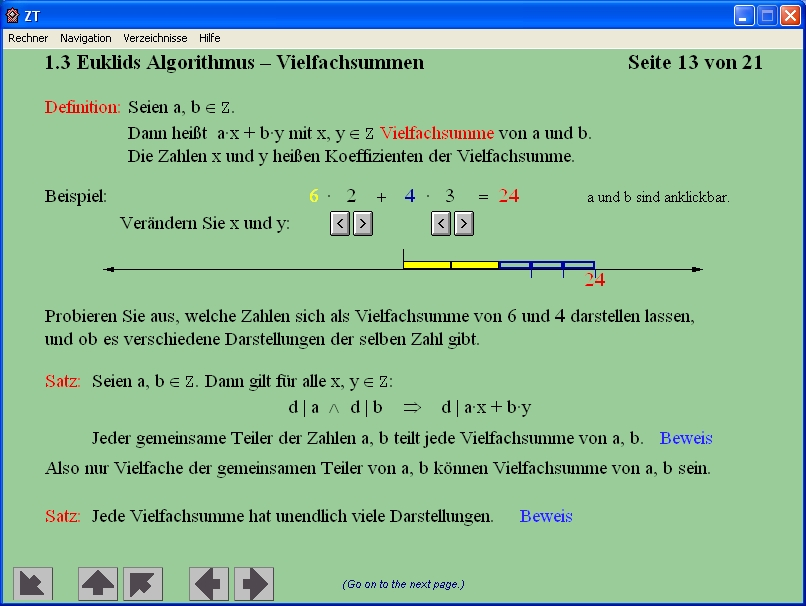
\includegraphics[scale=0.4]{figures/NT_Fig_C1-3_EuclidsAlg-LinearCombinations}
\caption{Jeder gemeinsame Teiler zweier Zahlen teilt auch alle ihre
Linearkombinationen\vspace{1ex}} 
\label{NT_Fig_C1.3_EuclidsAlg-LinearCombinations}
\end{center}
\end{figure}


\begin{figure}[ht]
\begin{center}
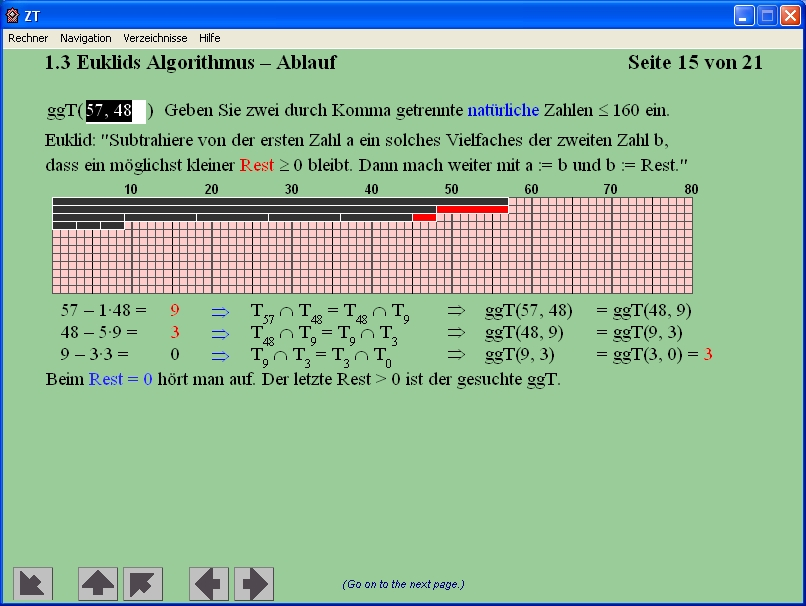
\includegraphics[scale=0.4]{figures/NT_Fig_C1-3_EuclidsAlg-Procedure}
\caption{Euklids Algorithmus zur Bestimmung des ggT\vspace{1ex}} 
\label{NT_Fig_C1.3_EuclidsAlg-Procedure}
\end{center}
\end{figure}


\begin{figure}[ht]
\begin{center}
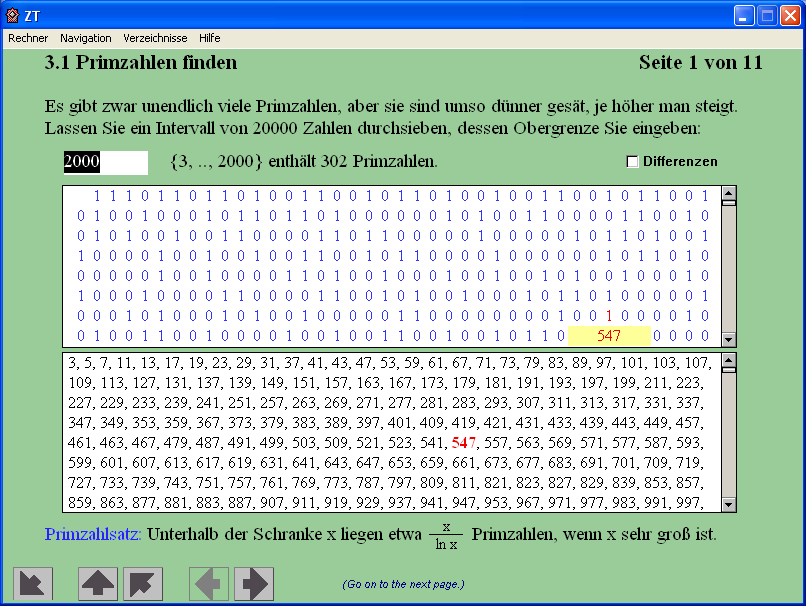
\includegraphics[scale=0.4]{figures/NT_Fig_C3-1_PrimesDistribution}
\caption{Verteilung der Primzahlen und ihrer Differenzen\vspace{1ex}} 
\label{NT_Fig_C3.1_PrimesDistribution}
\end{center}
\end{figure}


\begin{figure}[ht]
\begin{center}
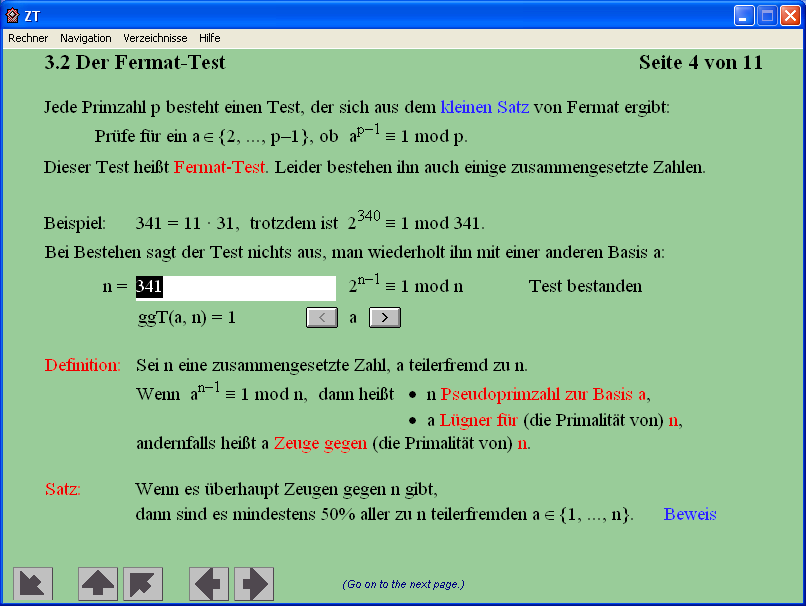
\includegraphics[scale=0.4]{figures/NT_Fig_C3-2_Fermat-Test}
\caption{Primzahlen finden mit dem Primzahltest nach Fermat\vspace{1ex}} 
\label{NT_Fig_C3.2_Fermat-Test}
\end{center}
\end{figure}


\begin{figure}[ht]
\begin{center}
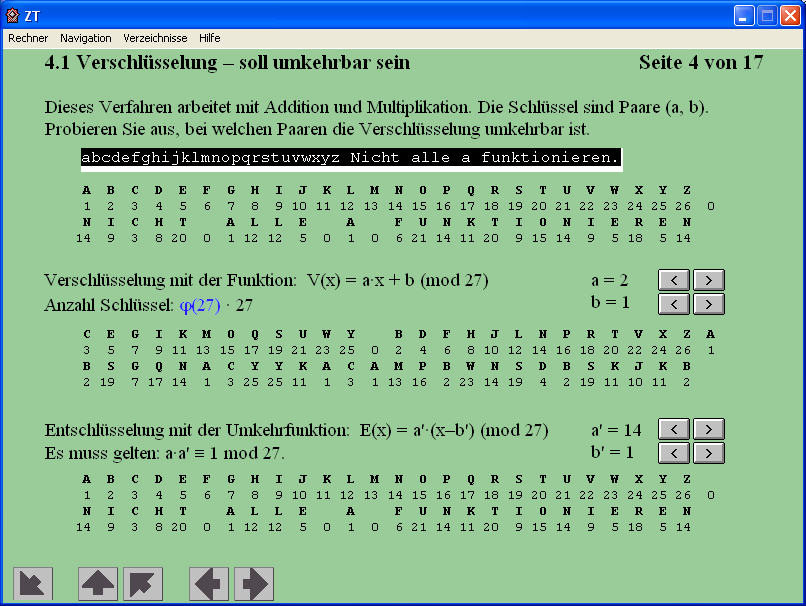
\includegraphics[scale=0.4]{figures/NT_Fig_C4-1_ReversibilityAdditiveCipher}
\caption{Umkehrbarkeit von Verschl�sselungsalgoritmen am Beispiel additiver Chiffren\vspace{1ex}} 
\label{NT_Fig_C4.1_ReversibilityAdditiveCipher}
\end{center}
\end{figure}


\begin{figure}[ht]
\begin{center}
\includegraphics[scale=0.4]{figures/NT_Fig_C5-2_Fermat-factorization-How-far-1}
\caption{Fermat-Faktorisierung m.H. der 3. Binomischen Formel\vspace{1ex}} 
\label{NT_Fig_C5.2_Fermat-factorization-How-far-1}
\end{center}
\end{figure}


\begin{figure}[ht]
\begin{center}
\includegraphics[scale=0.4]{figures/NT_Fig_C5-2_Fermat-factorization-How-far-2}
\caption{Fermat-Faktorisierung: Quadrate erkennen\vspace{1ex}} 
\label{NT_Fig_C5.2_Fermat-factorization-How-far-2}
\end{center}
\end{figure}


\begin{figure}[ht]
\begin{center}
\includegraphics[scale=0.4]{figures/NT_Fig_C5-3_PollardRho}
\caption{Pollards Rho-Faktorisierung: Kreisfindungsalgorithmus nach Floyd\vspace{1ex}} 
\label{NT_Fig_C5.3_PollardRho}
\end{center}
\end{figure}





% ++++++++++++++++++++++++++++++++++++++++++++++++++++++++++++++++++++++++++
\clearpage   % N�tig, damit Lit.verzeichnis nicht gl. nach Abb. 8 kommt.
% \newpage
\begin{thebibliography}{99999}
%\addcontentsline{toc}{section}{Literaturverzeichnis}

\bibitem[Buchmann2004]{a:Buchmann2004} \index{Buchmann 2004}
    Johannes Buchmann, \\
    {\em Einf�hrung in die Kryptographie}, Springer, 3. Auflage, 2004.

\bibitem[Scheid2003]{a:Scheid2003} \index{Scheid 2003}
    Harald Scheid, \\
    {\em Zahlentheorie}, Spektrum Akademischer Verlag, 3. Auflage, 2003.

\end{thebibliography}

%    \href{http://www....}
%    {\texttt{http://www....}}


  % ---------------------------------------------------------------------------
\newpage
\hypertarget{appendix-using-sage}{}
\section{Kurzeinf�hrung in das Computer-Algebra-System SageMath}
\label{s:appendix-using-sage}
\index{SageMath}
\index{SageMath!Programmbeispiele}

Dieses Buch enth�lt zahlreiche mit SageMath erstellte Programmbeispiele. SageMath ist
ein Open-Source Computer-Algebra-System (CAS), das f�r Lehre, Studium und Forschung
eingesetzt wird.
SageMath kombiniert viele hochwertige Open-Source-Packete\footnote{%
Einen Eindruck von der Gr��e von SageMath erh�lt man, wenn man es selbst compiliert:
Die heruntergeladenen Sourcen von SageMath 4.1 brauchten zur Compilierung auf einem
durchschnittlichen Linux-PC rund 5 h (inklusive aller Bibliotheken).
Danach nahm es 1,8 GB Plattenplatz ein.
}
und liefert den Zugang zu deren Funktionalit�t �ber ein gemeinsames, auf der
Programmiersprache Python basierendes Interface\footnote{%
Es gibt auch ein relativ einfaches Interface f�r die Sprache C, genannt Cython,
mit der man eigene Funktionen in SageMath stark beschleunigen kann.\\
Siehe \url{http://openwetware.org/wiki/Open_writing_projects/Sage_and_cython_a_brief_introduction}.
}.

\noindent SageMath kann man auf vielf�ltige Weise nutzen:
als m�chtigen Taschenrechner; als Tool f�r das Mathematikstudium;
oder als Programmier-Umgebung, um Algorithmen zu prototypen oder um Forschung im
Bereich der algorithmischen Aspekte der Mathematik zu betreiben.

\noindent Einen schnellen Einstieg bieten z.B. die Referenzen in dieser Fu�note%
\footnote{%
- \glqq Einladung zu Sage\grqq~von David Joyner, letztes Update 2009,\\
  \url{http://sage.math.washington.edu/home/wdj/teaching/calc1-sage/an-invitation-to-sage.pdf}\\
- \glqq The SDSU Sage Tutorial\grqq,\\
  \url{http://www-rohan.sdsu.edu/~mosulliv/sagetutorial/}\\
  \url{http://www-rohan.sdsu.edu/~mosulliv/sagetutorial/sagecalc.html}\\
- \glqq SAGE For Newbies\grqq~von Ted Kosan, 2007,\\
  \url{http://sage.math.washington.edu/home/tkosan/newbies_book/sage_for_newbies_v1.23.pdf}
}.
  
\noindent Die offizielle SageMath Online-Dokumentation\footnote{%
  Die entsprechenden offiziellen PDF-Dokuments k�nnen herunter geladen werden von\\
  \url{http://www.sagemath.org/help.html}, \url{http://www.sagemath.org/doc} und \url{http://planet.sagemath.org}.
} ist verf�gbar unter: \url{http://www.sagemath.org}.


\noindent Es gibt inzwischen viele PDF- und HTML-Dokumente �ber SageMath, so dass wir als guten Startpunkt nur einige wenige nennen\footnote{%
- \glqq Bibliothek\grqq: {\centering \url{http://www.sagemath.org/library/index.html}},\\
- \glqq Dokumentationsprojekt\grqq:
  {\centering \url{http://wiki.sagemath.org/DocumentationProject}},\\
- \glqq Lehrmaterial\grqq: {\centering \url{http://wiki.sagemath.org/Teaching_with_SAGE}}.
}.

\noindent Auch beim Studium der Kryptologie k�nnen fertige SageMath-Module genutzt
werden\footnote{%
- Sourcen der Module im Verzeichnis \url{SAGE_ROOT/devel/sage-main/sage/crypto}.

\noindent\hangindent=6pt\makebox[6pt][l]{-}�berblick,
   welche Kryptographie momentan in SageMath enthalten ist:\\
   \url{http://www.sagemath.org/doc/reference/sage/crypto/}

\noindent\hangindent=6pt\makebox[6pt][l]{-}Diskussionen
   �ber Lernaspekte beim Entwickeln weiterer Krypto-Module in SageMath:\\
   \url{http://groups.google.com/group/sage-devel/browse_thread/thread/c5572c4d8d42d081}
   % Leerzeile am Ende n�tig, sonst hat die zweite Zeile KEINEN h�ngenden Einzug?! (TODO)

}.

\noindent Umfangreiche Kryptographie-Einf�hrungen finden sich in der folgenden Fu�note\footnote{%
- Ein fertiger Kryptographie-Kurs von David Kohel, der SageMath nutzt, aus 2008:\\
{\centering \url{http://www.sagemath.org/library/crypto.pdf} }\\
bzw. derselbe Kurs in einer eventuell neueren Fassung\\
{\centering \url{http://sage.math.washington.edu/home/wdj/teaching/kohel-crypto.pdf} }.\\
- \glqq Introduction to Cryptography with Open-Source Software\grqq, ein
  hervorragendes Buch von Alasdair McAndrew, CRC, 2011
}.


% ---------------------------------------------------------------------------
\section*{SageMath-Benutzerschnittstellen}
SageMath ist kostenlos und kann von folgender Webseite herunter geladen werden:
\begin{center}
  \url{http://www.sagemath.org} \\
\end{center}
Standardm��ig nutzt man die SageMath-{\bf Kommandozeile} als Interface, wie im
folgenden Bild~\ref{fig:sage_cmd_interfaces} zu sehen ist.
Es gibt jedoch auch ein grafisches Benutzerinterface f�r diese Software
in Form des SageMath-Notebooks (siehe Bild~\ref{fig:sage_gui_interfaces}).
Und schlie�lich kann man SageMath-{\bf Notebooks}\footnote{%
Weitere Details zu SageMath-Notebooks finden Sie in
Kapitel~\ref{ec:Sage_Massierer} 
(\glqq \nameref{ec:Implementing-for-Education}\grqq
  $\Rightarrow$ \glqq \nameref{ec:Sage_Massierer}\grqq ).
                      }
auch online auf verschiedenen Servern nutzen, ohne SageMath lokal zu installieren, z.B.:
\begin{center}
\url{http://www.sagenb.org} oder \\
\url{http://sage.mathematik.uni-siegen.de:8000}
\end{center}

SageMath l�uft unter den Betriebssystemen Linux, Mac OS X und Windows.
Auf der Windows-Plattform l�uft die komplette SageMath-Distribution momentan
nur als ein VMware-Image.

\begin{figure}[!htpb]
\centering
\includegraphics[scale=0.6]{figures/sage-cmd}
\caption{SageMath-Kommandozeilen-Interface}
\label{fig:sage_cmd_interfaces}
\end{figure}

\begin{figure}[!htpb]
\centering
\includegraphics[scale=0.4]{figures/sage-gui}
\caption[SageMath-Notebook-Interface]{SageMath-Notebook-Interface\footnotemark}
\label{fig:sage_gui_interfaces}
\end{figure}

\footnotetext{%
Um das grafische SageMath-Interface lokal zu starten, muss man auf der SageMath-Kommandozeile
\verb#notebook()# eingeben. Danach startet der eingestellte Browser (Iceweasel,
Firefox, IE, ...) z.B. mit der URL \url{http://localhost:8000}.
}



% ---------------------------------------------------------------------------
\newpage
\section*{Hilfe beim Benutzen von SageMath}

Wenn man SageMath auf der Kommandozeile startet, erh�lt etwas wie die folgenden Zeilen:
%
\begin{Verbatim}%
[fontsize=\footnotesize]
mnemonic:~$ sage
----------------------------------------------------------------------
| Sage Version 4.1, Release Date: 2009-07-09                         |
| Type notebook() for the GUI, and license() for information.        |
----------------------------------------------------------------------

sage: help
Type help() for interactive help, or help(object) for help about object.
sage:
sage:
sage: help()

Welcome to Python 2.6!  This is the online help utility.

If this is your first time using Python, you should definitely check out
the tutorial on the Internet at http://docs.python.org/tutorial/.

Enter the name of any module, keyword, or topic to get help on writing
Python programs and using Python modules.  To quit this help utility and
return to the interpreter, just type "quit".

To get a list of available modules, keywords, or topics, type "modules",
"keywords", or "topics".  Each module also comes with a one-line summary
of what it does; to list the modules whose summaries contain a given word
such as "spam", type "modules spam".
\end{Verbatim}
%
Viele weitere Hilfen gibt es als offizielle SageMath-Dokumentation, die mit jedem
Release von SageMath verteilt wird~(siehe Bild~\ref{fig:sage_standard_doc}).
%
\begin{figure}[!htpb]
\centering
\includegraphics[scale=0.4]{figures/sage-online-doc}
\caption{Die Standard-Dokumentation von SageMath}
\label{fig:sage_standard_doc}
\end{figure}
%
Zur offiziellen SageMath-Standard-Dokumentation geh�ren folgende Dokumente:

\begin{itemize}
\item Tutorial --- Das Tutorial ist f�r SageMath-Einsteiger.
  Es ist daf�r gedacht, sich in ein bis drei Stunden mit den
  wichtigsten Funktionen vertraut zu machen.

\item Constructions --- Dieses Dokument ist im Stil eines \glqq Kochbuchs\grqq~mit
  einer Sammlung von Antworten auf Fragen zur Konstruktion von SageMath-Objekten.

\item Developers' Guide --- Dieser F�hrer ist f�r Entwickler, die selbst SageMath
  mit weiter entwickeln wollen. Enthalten sind darin z.B. Hinweise zum
  Stil und zu Konventionen beim Programmieren, zur Modifikation von
  SageMath-Kern-Bibliotheken oder von SageMath-Standard-Dokumentation, und zum Code-Review
  und zur Software-Verteilung.

\item Reference Manual --- Dieses Handbuch enth�lt die komplette Dokumentation
  aller wichtigen SageMath-Funktionen. Zu jeder Klassen-Beschreibung gibt es
  mehrere Code-Beispiele. Alle Code-Beispiele im Referenz-Handbuch werden
  bei jedem neuen SageMath-Release getestet.

\item Installation Guide --- Dieser F�hrer erkl�rt, wie man SageMath auf
  verschiedenen Plattformen installiert.

\item A Tour of Sage --- Diese Tour durch SageMath zeigt exemplarisch verschiedene
  Funktionen, die f�r Einsteiger sinnvoll sind.

\item Numerical Sage --- Dieses Dokument f�hrt Werkzeuge auf, die in SageMath
  f�r numerische Mathematik verf�gbar sind.

\item Three Lectures about Explicit Methods in Number Theory Using
  Sage --- Drei Vorlesungen �ber Methoden der Zahlentheorie, die explizit
  SageMath nutzen. Dieses Dokument zeigt wie man mit SageMath Berechnungen in
  fortgeschrittener Zahlentheorie durchf�hrt.
\end{itemize}

\noindent Von der SageMath-Kommandozeile erh�lt man eine Liste aller verf�gbaren Kommandos
(Funktionsnamen etc.), die ein bestimmtes Muster haben, wenn man die ersten Zeichen tippt,
und dann die \glqq Tab\grqq-Taste dr�ckt:
%
\begin{Verbatim}%
[fontsize=\footnotesize]
sage: Su[TAB]
Subsets                   Subwords                  SuzukiGroup
SubstitutionCryptosystem  SupersingularModule
\end{Verbatim}
%
Wenn man den genauen Namen eines Kommandos kennt, kann man die \texttt{help}-Funktion
nutzen oder das Fragezeichen \glqq ?\grqq~anf�gen, um weitere Informationen zu
diesem Kommando zu erhalten.  Zum Beispiel liefert das Kommando
\texttt{help(SubstitutionCryptosystem)} die Dokumentation zur der eingebauten
Klasse \texttt{SubstitutionCryptosystem}. Mit dem Fragezeichen erhalten wir die
Dokumentation zu dieser Klasse auf folgende Weise:
%
\begin{Verbatim}%
[fontsize=\footnotesize]
sage: SubstitutionCryptosystem?
Type:type
Base Class:<type 'type'>
String Form:<class 'sage.crypto.classical.SubstitutionCryptosystem'>
Namespace:Interactive
File:/home/mvngu/usr/bin/sage-3.4.1/local/lib/python2.5/site-packages/sage/crypto/classical.py
Docstring:

        Create a substitution cryptosystem.

        INPUT:

        - ``S`` - a string monoid over some alphabet

        OUTPUT:

        - A substitution cryptosystem over the alphabet ``S``.

        EXAMPLES::

            sage: M = AlphabeticStrings()
            sage: E = SubstitutionCryptosystem(M)
            sage: E
            Substitution cryptosystem on Free alphabetic string monoid
            on A-Z
            sage: K = M([ 25-i for i in range(26) ])
            sage: K
            ZYXWVUTSRQPONMLKJIHGFEDCBA
            sage: e = E(K)
            sage: m = M(``THECATINTHEHAT'')
            sage: e(m)
            GSVXZGRMGSVSZG

        TESTS::

            sage: M = AlphabeticStrings()
            sage: E = SubstitutionCryptosystem(M)
            sage: E == loads(dumps(E))
            True
\end{Verbatim}
%
\vspace{30pt}
Weitere Unterst�tzung f�r spezifische Probleme gibt es in den Archiven der
\texttt{sage-support} Mailing-Liste unter
%
\begin{center}
  \url{http://groups.google.com/group/sage-support}
\end{center}




% ---------------------------------------------------------------------------
\newpage
\section*{Beispiele f�r in SageMath eingebaute mathematische Funktionen}

Hier sind ein paar kleine Beispiele\footnote{%
Diese Beispiele stammen aus dem Blog von Dr. Alasdair McAndrew, Victoria University,\\
\url{http://amca01.wordpress.com/2008/12/19/sage-an-open-source-mathematics-software-system}}
(alle f�r das Kommandozeilen-Interface -- zur einfacheren Nutzung), um zu sehen,
was man mit SageMath machen kann:

\begin{sagecode}
\begin{Verbatim}%
[fontsize=\footnotesize]
# * Analysis (Infinitesimalrechnung):
    sage: x=var('x')
    sage: p=diff(exp(x^2),x,10)*exp(-x^2)
    sage: p.simplify_exp()
     1024 x^10 + 23040 x^8 + 161280 x^6 + 403200 x^4 + 302400 x^2 + 30240

# * Lineare Algebra:
    sage: M=matrix([[1,2,3],[4,5,6],[7,8,10]])
    sage: c=random_matrix(ZZ,3,1);c
     [ 7 ]
     [-2 ]
     [-2 ]
    sage: b=M*c
    sage: M^-1*b
     [ 7 ]
     [-2 ]
     [-2 ]

# * Zahlentheorie:
    sage: p=next_prime(randint(2^49,2^50));p
      1022095718672689
    sage: r=primitive_root(p);r
      7
    sage: pl=log(mod(10^15,p),r);pl
      1004868498084144
    sage: mod(r,p)^pl
      1000000000000000

# * Endliche K�rper (\url{http://de.wikipedia.org/wiki/Endlicher_K%C3%B6rper}):
    sage: F.<x>=GF(2)[]
    sage: G.<a>=GF(2^4,name='a',modulus=x^4+x+1)
    sage: a^2/(a^2+1)
      a^3 + a
    sage: a^100
      a^2 + a + 1
    sage: log(a^2,a^3+1)
      13
    sage: (a^3+1)^13
      a^2
\end{Verbatim}
\caption{Einige kleine Beispiele in SageMath aus verschiedenen Gebieten der Mathematik}
\end{sagecode}



% ---------------------------------------------------------------------------
\newpage
\section*{Programmieren mit SageMath}

Wenn man ein CAS (Computer-Algebra-System) nutzt, schreibt man zu Beginn einzelne
Befehle in die Kommandozeile wie im obigen Beispiel\footnote{%
  Standardm��ig wird SageMath-Code auch so pr�sentiert: Dabei beginnen die Zeilen
  mit  \glqq sage:\grqq~und \glqq ...\grqq.
  \begin{Verbatim}%
  [fontsize=\footnotesize]
  sage: m = 11
  sage: for a in xrange(1, m):
  ....:     print [power_mod(a, i, m) for i in xrange(1, m)]
  ....:
  \end{Verbatim}

  \noindent Auch dieses Skript benutzt normalerweise die obige Konvention, um
  SageMath-Code zu pr�sentieren, solange der Code nicht aus einer SageMath-Skriptdatei kommt.
  Wenn man den SageMath-Code aus diesem Skript kopiert und per Paste auf der SageMath-Kommandozeile
  wieder einf�gt, sollte man \glqq sage:\grqq~und \glqq ...\grqq~ weglassen
  (obwohl das Kommandozeilen-Interface in den meisten F�llen mit diesen Pr�fixen
  korrekt umgehen kann).}.

Wenn man eigene Funktionen entwickelt, sie �ndert und aufruft, dann ist es viel einfacher,
die Entwicklung in einem eigenen Editor vorzunehmen, den Code als SageMath-Skriptdatei zu
speichern und die Funktionen nicht-interaktiv auf der Kommandozeile auszuf�hren.
Beide Arten, Code zu entwickeln, wurden in
Kapitel \ref{CM_Sage_samples} (\glqq \nameref{CM_Sage_samples}\grqq),
Kapitel \ref{PaP_Sage_samples} (\glqq \nameref{PaP_Sage_samples}\grqq),
Kapitel \ref{primes:_Appendix_Sage-Samples} (\glqq \nameref{primes:_Appendix_Sage-Samples}\grqq)
und in Kapitel \ref{NumberTheory_Appendix_E} (\glqq\nameref{NumberTheory_Appendix_E}\grqq)
angewandt.

\noindent Um SageMath-Code in einem eigenen Editor zu entwickeln und zu testen, gibt es zwei
n�tzliche Befehle: \verb!load()! und \verb!attach()!\footnote{%
Vergleiche das SageMath-Tutorial �ber Programmierung, Kapitel
\glqq Loading and Attaching Sage files\grqq,\\
\url{http://www.sagemath.org/doc/tutorial/programming.html\#loading-and-attaching-sage-files}.}.\\
Angenommen Sie haben die folgende Funktions-Definition:
\begin{Verbatim}%
   [fontsize=\footnotesize]
   def function(var1):
       r"""
       DocText.
       """
       ...
       return (L)
\end{Verbatim}
\noindent die in der Datei \texttt{primroots.sage} gespeichert wurde.

\noindent Um diese Funktion in SageMath zu laden (und syntaktisch gleich zu testen),
wird der Befehl \verb!load()! benutzt:

\texttt{sage: load primroots.sage}

\noindent Danach kann man auf der Kommandozeile alle Variablen und Funktionen
nutzen, die im SageMath-Skript definiert wurden\footnote{%
Anmerkungen:

\noindent\hangindent=6pt\makebox[6pt][l]{-}Bitte keine Leerzeichen
oder White Spaces im Dateinamen.

\noindent\hangindent=6pt\makebox[6pt][l]{-}Es empfiehlt sich,
der SageMath-Skriptdatei die Datei-Extension
\glqq .sage\grqq~statt \glqq .py\grqq~zu geben.
Hat ein SageMath-Skript die Dateinamens-Endung \glqq .sage\grqq, dann wird
beim Laden der Datei in SageMath auch gleich die normale SageMath-Umgebung mit geladen,
um die Syntax zu pr�fen. Genauso funktioniert es, wenn man ein SageMath-Skript direkt
von einer Bash-Shell aufruft mit~~\texttt{\$ sage primroots.sage}.

\noindent\hangindent=6pt\makebox[6pt][l]{-}Beim Laden des obigen
SageMath-Skripts wird es von SageMath zuerst geparst, und dann
in eine andere Datei namens \glqq primroots.py\grqq~kopiert. SageMath erg�nzt
dann alle notwendigen Variablen in \glqq primroots.py\grqq~und alle Import-Statements.
Somit wird das SageMath-Skript genauso ausgef�hrt, als h�tte man die Befehle einzeln
auf der Kommandozeile eingetippt. Ein bedeutender Unterschied ist,
dass alle Ausgaben ein \verb!print!~ben�tigen.

}.

Normalerweise editiert man ein eigenes SageMath-Skript wieder und m�chte dann den
Inhalt des ge�nderten Skripts wieder in SageMath laden. Daf�r kann man den Befehl
\verb!attach()! nutzen (man kann auch direkt nach dem \verb!load()! 
das \verb!attach()! aufrufen, und nicht erst, wenn man das Skript �ndert;
man kann \verb!load()! sogar weglassen, da dies in \verb!attach()! enthalten ist):

\texttt{sage: attach primroots.sage}

Nun kann man das SageMath-Skript �ndern und die ge�nderte Funktionsdefinition
wird -- solange man die SageMath-Session nicht beendet -- beim n�chsten Enter
in SageMath geladen (und syntaktisch gleich gepr�ft). Diese Neuladen passiert
vollkommen automatisch. Der Befehl attach() l�sst SageMath also permanent die
genannte Datei auf �nderungen �berwachen. Damit spart man sich das Kopieren
und Pasten zwischen dem eigenen Texteditor und dem SageMath-Kommandozeilen-Interface.

Hier ist ein Bild, das SageMath-Code im Editor GVIM zeigt -- mit aktiviertem
Syntax-Highlighting (siehe Bild~\ref{fig:sage-highlighted-code-in-editor}).
%
\begin{figure}[!htpb]
\centering
\includegraphics[scale=0.7]{figures/sage-highlighted-code-in-editor}
\caption{SageMath-Beispiel in einem Editor mit aktiviertem Code-Highlighting}
\label{fig:sage-highlighted-code-in-editor}
\end{figure}

\vspace{20pt}
Falls man die Ausgabe einer attachten Datei so angezeigt haben m�chte,
wie wenn man die Einzelbefehle direkt auf der Kommandozeile eingibt
(also nicht nur das, was per \verb!print! ausgegeben wird),
kann man den Befehl \verb!iload()! verwenden:
Jede Zeile wird dann einzeln geladen. Um die n�chste Zeile zu laden,
muss man die \verb!Enter!-Taste dr�cken. Das muss man so lange wiederholen,
bis alle Zeilen des SageMath-Skripts in die SageMath-Session geladen sind.

\texttt{sage: iload primroots.sage}


% \vspace{30pt}
\newpage
\noindent Weitere Hinweise:
\begin{itemize}
  \item Abfrage der Version Ihrer SageMath-Umgebung mit: \texttt{version()}
  \item Um sich schnell die SageMath-Programmbeispiele in diesem Skript anzusehen, k�nnen Sie
    \begin{itemize}
      \item im Index nach \verb#SageMath -> Programmbeispiele# schauen, oder 
      \item sich im Anhang das \glqq \nameref{sc:List-of-Sage-Code-Examples}\grqq~ansehen.
    \end{itemize}
  \item Die SageMath-Beispiele in diesem Skript werden mit CrypTool ausgeliefert.\\
        Weitere Details am Ende der �bersicht
        \glqq \nameref{sc:List-of-Sage-Code-Examples}\grqq.
\end{itemize}



  % ++++++++++++++++++++++++++++++++++++++++++++++++++++++++++++++++++++++++++
\newpage
\hypertarget{appendix-authors}{}
\section{Authors of the CrypTool Book}\index{CrypTool}
\label{s:appendix-authors}

This appendix lists the authors\index{Authors} of this document.\\
Please refer to the top of each individual chapter for their contribution.

\begin{description}

\item[Bernhard Esslinger,] \mbox{}\\
Initiator of the CrypTool project, main author of this book. Professor for IT security and cryptography at the University of Siegen. Former CISO of SAP AG and head IT security at Deutsche Bank.\\
E-mail: bernhard.esslinger@gmail.com, bernhard.esslinger@uni-siegen.de

---------

\item[Matthias B\"uger,] \mbox{}\\ 
Contributor to chapter~\ref{Chapter_EllipticCurves} (``\nameref{Chapter_EllipticCurves}''),
research analyst at Deutsche Bank.

\item[Bartol Filipovic,] \mbox{}\\
Original author of the CrypTool elliptic curve
implementation and the corresponding chapter in this book.

\item[Martin Franz,] \mbox{}\\
Author of chapter~\ref{Chapter_HomomorphicCiphers}
(``\nameref{Chapter_HomomorphicCiphers}'').
Works and carries out research in the area of applied cryptography.

\item[Henrik Koy,] \mbox{}\\
Main developer and co-ordinator of CT1 development
since version 1.3; book reviewer and \TeX\ guru; cryptographer 
and project leader IT at Deutsche Bank.

\item[Roger Oyono,] \mbox{}\\
Implementer of the CT1 factorization dialog and original author
of chapter~\ref{Chapter_ModernCryptography} (``\nameref{Chapter_ModernCryptography}'').

\item[Klaus Pommerening,] \mbox{}\\
Author of chapter~\ref{Chapter_BitCiphers} (``\nameref{Chapter_BitCiphers}''), 
Professor for mathematics and computer science at Johannes-Gutenberg-Universit\"at. Retired.

\item[J\"org Cornelius Schneider,] \mbox{}\\
Design and support of CrypTool; crypto enthusiast, IT architect and
senior project leader IT at Deutsche Bank.

\item[Christine St\"otzel,] \mbox{}\\
Master of Business and Computer Science at the University of Siegen.

---------

\item[Johannes Buchmann,] \mbox{}\\
Co-author of chapter~\ref{Chapter_Crypto2020} (``\nameref{Chapter_Crypto2020}'').
%Vice-president of the Technische Universit\"at Darmstadt, Germany and
%Professor at the Departments of Computer Science and of Mathematics.
Johannes Buchmann holds the Chair for Theoretical Computer Science (Cryptography
and Computer Algebra) at the department of Computer Science of the Technische
Universit\"at Darmstadt TUD).  He is also a Professor at the department of Mathematics, and vice-president of the university.

\item[Alexander May,] \mbox{}\\
Co-author of chapter~\ref{Chapter_Crypto2020} (``\nameref{Chapter_Crypto2020}''), 
Professor at the department of mathematics (chair for cryptology and
IT Security) of the Ruhr-Universit\"at Bochum.


\item[Erik Dahmen,] \mbox{}\\
Co-author of chapter~\ref{Chapter_Crypto2020} (``\nameref{Chapter_Crypto2020}''). 
%Researcher at the Department of Computer Science of the TUD.
Researcher at the Chair for Theoretical Computer Science (Cryptography and
Computer Algebra), department of Computer Science, Technische Universit\"at
Darmstadt, Germany.

\item[Ulrich Vollmer,] \mbox{}\\
Co-author of chapter~\ref{Chapter_Crypto2020} (``\nameref{Chapter_Crypto2020}'').
Researcher at the Chair for Theoretical Computer Science (Cryptography and
Computer Algebra), department of Computer Science, Technische Universit\"at
Darmstadt, Germany.

---------

\item[Minh Van Nguyen,] \mbox{}\\
SageMath developer and documentation quality reviewer.



\end{description}


\end{appendix}

% This is set up to run with pdflatex.
%---------The file header---------------------------------------------
% \documentclass[a4paper,12pt]{book}

% \usepackage[english]{babel} %language selection
% \selectlanguage{english}

% \pagenumbering{arabic}

% \usepackage{hyperref}
% \hypersetup{colorlinks,
%            citecolor=black,
%            filecolor=black,
%            linkcolor=black,
%            urlcolor=black,
%            bookmarksopen=true,
%            pdftex}

% \hfuzz = .6pt % avoid black boxes

% \begin{document}
%---------------------------------------------------------------------
\clearpage\phantomsection
\addcontentsline{toc}{chapter}{GNU Free Documentation License}
\chapter*{\rlap{GNU Free Documentation License}}
%\label{label_fdl}
\hypertarget{appendix-GNU-fdl}{}
\label{s:appendix-GNU-fdl}

\begin{center}

       Version 1.3, 3 November 2008


 Copyright \copyright{} 2000, 2001, 2002, 2007, 2008  Free Software Foundation, Inc.

 \bigskip

     \url{http://fsf.org/}

 \bigskip

 Everyone is permitted to copy and distribute verbatim copies
 of this license document, but changing it is not allowed.
\end{center}


\begin{center}
{\bf\large Preamble}
\end{center}

The purpose of this License is to make a manual, textbook, or other
functional and useful document ``free'' in the sense of freedom: to
assure everyone the effective freedom to copy and redistribute it,
with or without modifying it, either commercially or noncommercially.
Secondarily, this License preserves for the author and publisher a way
to get credit for their work, while not being considered responsible
for modifications made by others.

This License is a kind of ``copyleft'', which means that derivative
works of the document must themselves be free in the same sense.  It
complements the GNU General Public License, which is a copyleft
license designed for free software.

We have designed this License in order to use it for manuals for free
software, because free software needs free documentation: a free
program should come with manuals providing the same freedoms that the
software does.  But this License is not limited to software manuals;
it can be used for any textual work, regardless of subject matter or
whether it is published as a printed book.  We recommend this License
principally for works whose purpose is instruction or reference.


\begin{center}
{\Large\bf 1. APPLICABILITY AND DEFINITIONS\par}
% \phantomsection
% \addcontentsline{toc}{chapter}{1. APPLICABILITY AND DEFINITIONS}
\end{center}

This License applies to any manual or other work, in any medium, that
contains a notice placed by the copyright holder saying it can be
distributed under the terms of this License.  Such a notice grants a
world-wide, royalty-free license, unlimited in duration, to use that
work under the conditions stated herein.  The ``\textbf{Document}'', below,
refers to any such manual or work.  Any member of the public is a
licensee, and is addressed as ``\textbf{you}''.  You accept the license if you
copy, modify or distribute the work in a way requiring permission
under copyright law.

A ``\textbf{Modified Version}'' of the Document means any work containing the
Document or a portion of it, either copied verbatim, or with
modifications and/or translated into another language.

A ``\textbf{Secondary Section}'' is a named appendix or a front-matter section of
the Document that deals exclusively with the relationship of the
publishers or authors of the Document to the Document's overall subject
(or to related matters) and contains nothing that could fall directly
within that overall subject.  (Thus, if the Document is in part a
textbook of mathematics, a Secondary Section may not explain any
mathematics.)  The relationship could be a matter of historical
connection with the subject or with related matters, or of legal,
commercial, philosophical, ethical or political position regarding
them.

The ``\textbf{Invariant Sections}'' are certain Secondary Sections whose titles
are designated, as being those of Invariant Sections, in the notice
that says that the Document is released under this License.  If a
section does not fit the above definition of Secondary then it is not
allowed to be designated as Invariant.  The Document may contain zero
Invariant Sections.  If the Document does not identify any Invariant
Sections then there are none.

The ``\textbf{Cover Texts}'' are certain short passages of text that are listed,
as Front-Cover Texts or Back-Cover Texts, in the notice that says that
the Document is released under this License.  A Front-Cover Text may
be at most 5 words, and a Back-Cover Text may be at most 25 words.

A ``\textbf{Transparent}'' copy of the Document means a machine-readable copy,
represented in a format whose specification is available to the
general public, that is suitable for revising the document
straightforwardly with generic text editors or (for images composed of
pixels) generic paint programs or (for drawings) some widely available
drawing editor, and that is suitable for input to text formatters or
for automatic translation to a variety of formats suitable for input
to text formatters.  A copy made in an otherwise Transparent file
format whose markup, or absence of markup, has been arranged to thwart
or discourage subsequent modification by readers is not Transparent.
An image format is not Transparent if used for any substantial amount
of text.  A copy that is not ``Transparent'' is called ``\textbf{Opaque}''.

Examples of suitable formats for Transparent copies include plain
ASCII without markup, Texinfo input format, LaTeX input format, SGML
or XML using a publicly available DTD, and standard-conforming simple
HTML, PostScript or PDF designed for human modification.  Examples of
transparent image formats include PNG, XCF and JPG.  Opaque formats
include proprietary formats that can be read and edited only by
proprietary word processors, SGML or XML for which the DTD and/or
processing tools are not generally available, and the
machine-generated HTML, PostScript or PDF produced by some word
processors for output purposes only.

The ``\textbf{Title Page}'' means, for a printed book, the title page itself,
plus such following pages as are needed to hold, legibly, the material
this License requires to appear in the title page.  For works in
formats which do not have any title page as such, ``Title Page'' means
the text near the most prominent appearance of the work's title,
preceding the beginning of the body of the text.

The ``\textbf{publisher}'' means any person or entity that distributes
copies of the Document to the public.

A section ``\textbf{Entitled XYZ}'' means a named subunit of the Document whose
title either is precisely XYZ or contains XYZ in parentheses following
text that translates XYZ in another language.  (Here XYZ stands for a
specific section name mentioned below, such as ``\textbf{Acknowledgements}'',
``\textbf{Dedications}'', ``\textbf{Endorsements}'', or ``\textbf{History}''.)
To ``\textbf{Preserve the Title}''
of such a section when you modify the Document means that it remains a
section ``Entitled XYZ'' according to this definition.

The Document may include Warranty Disclaimers next to the notice which
states that this License applies to the Document.  These Warranty
Disclaimers are considered to be included by reference in this
License, but only as regards disclaiming warranties: any other
implication that these Warranty Disclaimers may have is void and has
no effect on the meaning of this License.


\begin{center}
{\Large\bf 2. VERBATIM COPYING\par}
% \phantomsection
% \addcontentsline{toc}{chapter}{2. VERBATIM COPYING}
\end{center}

You may copy and distribute the Document in any medium, either
commercially or noncommercially, provided that this License, the
copyright notices, and the license notice saying this License applies
to the Document are reproduced in all copies, and that you add no other
conditions whatsoever to those of this License.  You may not use
technical measures to obstruct or control the reading or further
copying of the copies you make or distribute.  However, you may accept
compensation in exchange for copies.  If you distribute a large enough
number of copies you must also follow the conditions in section~3.

You may also lend copies, under the same conditions stated above, and
you may publicly display copies.


\begin{center}
{\Large\bf 3. COPYING IN QUANTITY\par}
% \phantomsection
% \addcontentsline{toc}{chapter}{3. COPYING IN QUANTITY}
\end{center}


If you publish printed copies (or copies in media that commonly have
printed covers) of the Document, numbering more than 100, and the
Document's license notice requires Cover Texts, you must enclose the
copies in covers that carry, clearly and legibly, all these Cover
Texts: Front-Cover Texts on the front cover, and Back-Cover Texts on
the back cover.  Both covers must also clearly and legibly identify
you as the publisher of these copies.  The front cover must present
the full title with all words of the title equally prominent and
visible.  You may add other material on the covers in addition.
Copying with changes limited to the covers, as long as they preserve
the title of the Document and satisfy these conditions, can be treated
as verbatim copying in other respects.

If the required texts for either cover are too voluminous to fit
legibly, you should put the first ones listed (as many as fit
reasonably) on the actual cover, and continue the rest onto adjacent
pages.

If you publish or distribute Opaque copies of the Document numbering
more than 100, you must either include a machine-readable Transparent
copy along with each Opaque copy, or state in or with each Opaque copy
a computer-network location from which the general network-using
public has access to download using public-standard network protocols
a complete Transparent copy of the Document, free of added material.
If you use the latter option, you must take reasonably prudent steps,
when you begin distribution of Opaque copies in quantity, to ensure
that this Transparent copy will remain thus accessible at the stated
location until at least one year after the last time you distribute an
Opaque copy (directly or through your agents or retailers) of that
edition to the public.

It is requested, but not required, that you contact the authors of the
Document well before redistributing any large number of copies, to give
them a chance to provide you with an updated version of the Document.


\begin{center}
{\Large\bf 4. MODIFICATIONS\par}
% \phantomsection
% \addcontentsline{toc}{chapter}{4. MODIFICATIONS}
\end{center}

You may copy and distribute a Modified Version of the Document under
the conditions of sections 2 and 3 above, provided that you release
the Modified Version under precisely this License, with the Modified
Version filling the role of the Document, thus licensing distribution
and modification of the Modified Version to whoever possesses a copy
of it.  In addition, you must do these things in the Modified Version:

\begin{itemize}
\item[A.]
   Use in the Title Page (and on the covers, if any) a title distinct
   from that of the Document, and from those of previous versions
   (which should, if there were any, be listed in the History section
   of the Document).  You may use the same title as a previous version
   if the original publisher of that version gives permission.

\item[B.]
   List on the Title Page, as authors, one or more persons or entities
   responsible for authorship of the modifications in the Modified
   Version, together with at least five of the principal authors of the
   Document (all of its principal authors, if it has fewer than five),
   unless they release you from this requirement.

\item[C.]
   State on the Title page the name of the publisher of the
   Modified Version, as the publisher.

\item[D.]
   Preserve all the copyright notices of the Document.

\item[E.]
   Add an appropriate copyright notice for your modifications
   adjacent to the other copyright notices.

\item[F.]
   Include, immediately after the copyright notices, a license notice
   giving the public permission to use the Modified Version under the
   terms of this License, in the form shown in the Addendum below.

\item[G.]
   Preserve in that license notice the full lists of Invariant Sections
   and required Cover Texts given in the Document's license notice.

\item[H.]
   Include an unaltered copy of this License.

\item[I.]
   Preserve the section Entitled ``History'', Preserve its Title, and add
   to it an item stating at least the title, year, new authors, and
   publisher of the Modified Version as given on the Title Page.  If
   there is no section Entitled ``History'' in the Document, create one
   stating the title, year, authors, and publisher of the Document as
   given on its Title Page, then add an item describing the Modified
   Version as stated in the previous sentence.

\item[J.]
   Preserve the network location, if any, given in the Document for
   public access to a Transparent copy of the Document, and likewise
   the network locations given in the Document for previous versions
   it was based on.  These may be placed in the ``History'' section.
   You may omit a network location for a work that was published at
   least four years before the Document itself, or if the original
   publisher of the version it refers to gives permission.

\item[K.]
   For any section Entitled ``Acknowledgements'' or ``Dedications'',
   Preserve the Title of the section, and preserve in the section all
   the substance and tone of each of the contributor acknowledgements
   and/or dedications given therein.

\item[L.]
   Preserve all the Invariant Sections of the Document,
   unaltered in their text and in their titles.  Section numbers
   or the equivalent are not considered part of the section titles.

\item[M.]
   Delete any section Entitled ``Endorsements''.  Such a section
   may not be included in the Modified Version.

\item[N.]
   Do not retitle any existing section to be Entitled ``Endorsements''
   or to conflict in title with any Invariant Section.

\item[O.]
   Preserve any Warranty Disclaimers.
\end{itemize}

If the Modified Version includes new front-matter sections or
appendices that qualify as Secondary Sections and contain no material
copied from the Document, you may at your option designate some or all
of these sections as invariant.  To do this, add their titles to the
list of Invariant Sections in the Modified Version's license notice.
These titles must be distinct from any other section titles.

You may add a section Entitled ``Endorsements'', provided it contains
nothing but endorsements of your Modified Version by various
parties---for example, statements of peer review or that the text has
been approved by an organization as the authoritative definition of a
standard.

You may add a passage of up to five words as a Front-Cover Text, and a
passage of up to 25 words as a Back-Cover Text, to the end of the list
of Cover Texts in the Modified Version.  Only one passage of
Front-Cover Text and one of Back-Cover Text may be added by (or
through arrangements made by) any one entity.  If the Document already
includes a cover text for the same cover, previously added by you or
by arrangement made by the same entity you are acting on behalf of,
you may not add another; but you may replace the old one, on explicit
permission from the previous publisher that added the old one.

The author(s) and publisher(s) of the Document do not by this License
give permission to use their names for publicity for or to assert or
imply endorsement of any Modified Version.


\begin{center}
{\Large\bf 5. COMBINING DOCUMENTS\par}
% \phantomsection
% \addcontentsline{toc}{chapter}{5. COMBINING DOCUMENTS}
\end{center}


You may combine the Document with other documents released under this
License, under the terms defined in section~4 above for modified
versions, provided that you include in the combination all of the
Invariant Sections of all of the original documents, unmodified, and
list them all as Invariant Sections of your combined work in its
license notice, and that you preserve all their Warranty Disclaimers.

The combined work need only contain one copy of this License, and
multiple identical Invariant Sections may be replaced with a single
copy.  If there are multiple Invariant Sections with the same name but
different contents, make the title of each such section unique by
adding at the end of it, in parentheses, the name of the original
author or publisher of that section if known, or else a unique number.
Make the same adjustment to the section titles in the list of
Invariant Sections in the license notice of the combined work.

In the combination, you must combine any sections Entitled ``History''
in the various original documents, forming one section Entitled
``History''; likewise combine any sections Entitled ``Acknowledgements'',
and any sections Entitled ``Dedications''.  You must delete all sections
Entitled ``Endorsements''.

\begin{center}
{\Large\bf 6. COLLECTIONS OF DOCUMENTS\par}
% \phantomsection
% \addcontentsline{toc}{chapter}{6. COLLECTIONS OF DOCUMENTS}
\end{center}

You may make a collection consisting of the Document and other documents
released under this License, and replace the individual copies of this
License in the various documents with a single copy that is included in
the collection, provided that you follow the rules of this License for
verbatim copying of each of the documents in all other respects.

You may extract a single document from such a collection, and distribute
it individually under this License, provided you insert a copy of this
License into the extracted document, and follow this License in all
other respects regarding verbatim copying of that document.


\begin{center}
{\Large\bf 7. AGGREGATION WITH INDEPENDENT WORKS\par}
% \phantomsection
% \addcontentsline{toc}{chapter}{7. AGGREGATION WITH INDEPENDENT WORKS}
\end{center}


A compilation of the Document or its derivatives with other separate
and independent documents or works, in or on a volume of a storage or
distribution medium, is called an ``aggregate'' if the copyright
resulting from the compilation is not used to limit the legal rights
of the compilation's users beyond what the individual works permit.
When the Document is included in an aggregate, this License does not
apply to the other works in the aggregate which are not themselves
derivative works of the Document.

If the Cover Text requirement of section~3 is applicable to these
copies of the Document, then if the Document is less than one half of
the entire aggregate, the Document's Cover Texts may be placed on
covers that bracket the Document within the aggregate, or the
electronic equivalent of covers if the Document is in electronic form.
Otherwise they must appear on printed covers that bracket the whole
aggregate.


\begin{center}
{\Large\bf 8. TRANSLATION\par}
% \phantomsection
% \addcontentsline{toc}{chapter}{8. TRANSLATION}
\end{center}


Translation is considered a kind of modification, so you may
distribute translations of the Document under the terms of section~4.
Replacing Invariant Sections with translations requires special
permission from their copyright holders, but you may include
translations of some or all Invariant Sections in addition to the
original versions of these Invariant Sections.  You may include a
translation of this License, and all the license notices in the
Document, and any Warranty Disclaimers, provided that you also include
the original English version of this License and the original versions
of those notices and disclaimers.  In case of a disagreement between
the translation and the original version of this License or a notice
or disclaimer, the original version will prevail.

If a section in the Document is Entitled ``Acknowledgements'',
``Dedications'', or ``History'', the requirement (section~4) to Preserve
its Title (section~1) will typically require changing the actual
title.


\begin{center}
{\Large\bf 9. TERMINATION\par}
% \phantomsection
% \addcontentsline{toc}{chapter}{9. TERMINATION}
\end{center}


You may not copy, modify, sublicense, or distribute the Document
except as expressly provided under this License.  Any attempt
otherwise to copy, modify, sublicense, or distribute it is void, and
will automatically terminate your rights under this License.

However, if you cease all violation of this License, then your license
from a particular copyright holder is reinstated (a) provisionally,
unless and until the copyright holder explicitly and finally
terminates your license, and (b) permanently, if the copyright holder
fails to notify you of the violation by some reasonable means prior to
60 days after the cessation.

Moreover, your license from a particular copyright holder is
reinstated permanently if the copyright holder notifies you of the
violation by some reasonable means, this is the first time you have
received notice of violation of this License (for any work) from that
copyright holder, and you cure the violation prior to 30 days after
your receipt of the notice.

Termination of your rights under this section does not terminate the
licenses of parties who have received copies or rights from you under
this License.  If your rights have been terminated and not permanently
reinstated, receipt of a copy of some or all of the same material does
not give you any rights to use it.


\begin{center}
{\Large\bf 10. FUTURE REVISIONS OF THIS LICENSE\par}
% \phantomsection
% \addcontentsline{toc}{chapter}{10. FUTURE REVISIONS OF THIS LICENSE}
\end{center}


The Free Software Foundation may publish new, revised versions
of the GNU Free Documentation License from time to time.  Such new
versions will be similar in spirit to the present version, but may
differ in detail to address new problems or concerns.  See
\url{http://www.gnu.org/copyleft/}.

Each version of the License is given a distinguishing version number.
If the Document specifies that a particular numbered version of this
License ``or any later version'' applies to it, you have the option of
following the terms and conditions either of that specified version or
of any later version that has been published (not as a draft) by the
Free Software Foundation.  If the Document does not specify a version
number of this License, you may choose any version ever published (not
as a draft) by the Free Software Foundation.  If the Document
specifies that a proxy can decide which future versions of this
License can be used, that proxy's public statement of acceptance of a
version permanently authorizes you to choose that version for the
Document.


\begin{center}
{\Large\bf 11. RELICENSING\par}
% \phantomsection
% \addcontentsline{toc}{chapter}{11. RELICENSING}
\end{center}


``Massive Multiauthor Collaboration Site'' (or ``MMC Site'') means any
World Wide Web server that publishes copyrightable works and also
provides prominent facilities for anybody to edit those works.  A
public wiki that anybody can edit is an example of such a server.  A
``Massive Multiauthor Collaboration'' (or ``MMC'') contained in the
site means any set of copyrightable works thus published on the MMC
site.

``CC-BY-SA'' means the Creative Commons Attribution-Share Alike 3.0
license published by Creative Commons Corporation, a not-for-profit
corporation with a principal place of business in San Francisco,
California, as well as future copyleft versions of that license
published by that same organization.

``Incorporate'' means to publish or republish a Document, in whole or
in part, as part of another Document.

An MMC is ``eligible for relicensing'' if it is licensed under this
License, and if all works that were first published under this License
somewhere other than this MMC, and subsequently incorporated in whole
or in part into the MMC, (1) had no cover texts or invariant sections,
and (2) were thus incorporated prior to November 1, 2008.

The operator of an MMC Site may republish an MMC contained in the site
under CC-BY-SA on the same site at any time before August 1, 2009,
provided the MMC is eligible for relicensing.


\begin{center}
{\Large\bf ADDENDUM: How to use this License for your documents\par}
% \phantomsection
% \addcontentsline{toc}{chapter}{ADDENDUM: How to use this License for your documents}
\end{center}

To use this License in a document you have written, include a copy of
the License in the document and put the following copyright and
license notices just after the title page:

\bigskip
\begin{quote}
    Copyright \copyright{}  YEAR  YOUR NAME.
    Permission is granted to copy, distribute and/or modify this document
    under the terms of the GNU Free Documentation License, Version 1.3
    or any later version published by the Free Software Foundation;
    with no Invariant Sections, no Front-Cover Texts, and no Back-Cover Texts.
    A copy of the license is included in the section entitled ``GNU
    Free Documentation License''.
\end{quote}
\bigskip

If you have Invariant Sections, Front-Cover Texts and Back-Cover Texts,
replace the ``with \dots\ Texts.'' line with this:

\bigskip
\begin{quote}
    with the Invariant Sections being LIST THEIR TITLES, with the
    Front-Cover Texts being LIST, and with the Back-Cover Texts being LIST.
\end{quote}
\bigskip

If you have Invariant Sections without Cover Texts, or some other
combination of the three, merge those two alternatives to suit the
situation.

If your document contains nontrivial examples of program code, we
recommend releasing these examples in parallel under your choice of
free software license, such as the GNU General Public License,
to permit their use in free software.

%---------------------------------------------------------------------
% \end{document}



% ++++++++++++++++++++++++++++++++++++++++++++++++++++++++++++++++++++++++++
\begingroup
  % remove extra vertical space from \listoffigure and \listoftables so that 
  % it looks similar to \listof{sagecode}
  \setlength{\parskip}{0pt}

  \clearpage\phantomsection
  \addcontentsline{toc}{chapter}{\listfigurename}
  \listoffigures

  \clearpage\phantomsection
  \addcontentsline{toc}{chapter}{\listtablename}
  \listoftables

  \clearpage\phantomsection
  \addcontentsline{toc}{chapter}{Verzeichnis der Krypto-Verfahren mit Pseudocode}
  \listof{cryptoprocedure}{Verzeichnis der Krypto-Verfahren mit Pseudocode}
\endgroup


\clearpage\phantomsection
\addcontentsline{toc}{chapter}{Verzeichnis der Zitate}
\listof{ctsquotefloat}{Verzeichnis der Zitate}
\index{Zitate}
\label{sc:List-of-Quotes}


\clearpage\phantomsection
\addcontentsline{toc}{chapter}{Verzeichnis der SageMath-Programmbeispiele}
\listof{sagecode}{Verzeichnis der SageMath-Programmbeispiele}
\index{SageMath!Programmbeispiele}
\label{sc:List-of-Sage-Code-Examples}
% \hypertarget{sc:List-of-Sage-Code-Examples}{}

\vspace{30pt}
\begin{itemize}
  \item Der Quellcode der SageMath-Beispiele in diesem Skript wird in Form von
        SageMath-Programmdatei"-en mit dem CrypTool 1-Setup-Programm ausgeliefert.
        Die Beispiele in einem Kapitel sind jeweils in einer Datei zusammen gefasst.\\
        Nach der Installation von CrypTool 1 \index{CrypTool 1} finden Sie
        die SageMath-Beispiele im Unterverzeichnis \verb#sagemath# in den folgenden
        4 Dateien:\\
        - SageMath-Samples-in-Chap01.sage \\
        - SageMath-Samples-in-Chap02.sage \\
        - SageMath-Samples-in-Chap03.sage \\
        - SageMath-Samples-in-Chap04.sage
  \item Alle Beispiel wurden mit der SageMath-Version 5.3 (Release Date 2012-09-08) xxxxxxxxxxxxxxxxxxxx  getestet.
\end{itemize}   % xxxxxxxxxxxxxx Weitere Beispiele erg�nzen !


\clearpage\phantomsection
\addcontentsline{toc}{chapter}{Index}
\printindex

\newpage %Nice-to-have-TODO_Doesn't seem to create an empty page at the end.
\newpage

\end{document}


